% $Header$
% MBDyn (C) is a multibody analysis code.
% http://www.mbdyn.org
%
% Copyright (C) 1996-2023
%
% Pierangelo Masarati  <pierangelo.masarati@polimi.it>
%
% Dipartimento di Ingegneria Aerospaziale - Politecnico di Milano
% via La Masa, 34 - 20156 Milano, Italy
% http://www.aero.polimi.it
%
% Changing this copyright notice is forbidden.
%
% This program is free software; you can redistribute it and/or modify
% it under the terms of the GNU General Public License as published by
% the Free Software Foundation (version 2 of the License).
% 
%
% This program is distributed in the hope that it will be useful,
% but WITHOUT ANY WARRANTY; without even the implied warranty of
% MERCHANTABILITY or FITNESS FOR A PARTICULAR PURPOSE.  See the
% GNU General Public License for more details.
%
% You should have received a copy of the GNU General Public License
% along with this program; if not, write to the Free Software
% Foundation, Inc., 59 Temple Place, Suite 330, Boston, MA  02111-1307  USA

\documentclass[10pt]{report}

%\usepackage[pdftex]{graphicx}
\usepackage[T1]{fontenc}
\usepackage{ae,aecompl}
\usepackage{graphicx}
\usepackage{psfrag}
\usepackage{amsmath}
\usepackage{amssymb}
\usepackage{bm}
\usepackage[breaklinks=true,colorlinks=false]{hyperref}
\usepackage{html}
\usepackage{comment}
\usepackage{moreverb}
\usepackage{fancyvrb}
\usepackage{xcolor}
\usepackage{framed}
\usepackage{enumitem}
\usepackage{subcaption}
\DeclareMathOperator{\trace}{trace}
% $Header$
% Copyright (C) 1996-2023 Pierangelo Masarati <pierangelo.masarati@polimi.it>
% Dipartimento di Ingegneria Aerospaziale, Politecnico di Milano
%
% Parentesi: tonde, quadre, curly, dritte, doppie e angolari.
\newcommand{\plbr}[1]{ \left( #1 \right) }
\newcommand{\sqbr}[1]{ \left[ #1 \right] }
\newcommand{\cubr}[1]{ \left\{ #1 \right\} }
\newcommand{\shbr}[1]{ \left| #1 \right| }
\newcommand{\nrbr}[1]{ \left\| #1 \right\| }
\newcommand{\anbr}[1]{ \langle #1 \rangle }

% Parentesi solo a sinistra: tonde, quadre, curly, dritte, doppie e angolari.
\newcommand{\lplbr}[1]{ \left( #1 \right. }
\newcommand{\lsqbr}[1]{ \left[ #1 \right. }
\newcommand{\lcubr}[1]{ \left\{ #1 \right. }
\newcommand{\lshbr}[1]{ \left| #1 \right. }
\newcommand{\lnrbr}[1]{ \left\| #1 \right. }
\newcommand{\lanbr}[1]{ \langle #1 \right. }

% Parentesi solo a destra: tonde, quadre, curly, dritte,doppie e angolari.
\newcommand{\rplbr}[1]{ \left. #1 \right) }
\newcommand{\rsqbr}[1]{ \left. #1 \right] }
\newcommand{\rcubr}[1]{ \left. #1 \right\} }
\newcommand{\rshbr}[1]{ \left. #1 \right| }
\newcommand{\rnrbr}[1]{ \left. #1 \right\| }
\newcommand{\ranbr}[1]{ \left. #1 \rangle }

% Vettori verticali:
\newcommand{\vvect}[2]{ \begin{array}{ #1 } #2 \end{array} }
\newcommand{\cvvect}[1]{ \begin{array}{c} #1 \end{array} }
\newcommand{\lvvect}[1]{ \begin{array}{l} #1 \end{array} }
\newcommand{\rvvect}[1]{ \begin{array}{r} #1 \end{array} }

% Vettori orizzontali:
\newcommand{\hvect}[2]{ \begin{array}{ #1 } #2 \end{array} }

% Matrici:
\newcommand{\matr}[2]{ \begin{array}{ #1 } #2 \end{array} }

% Integrali: uso \intg{inf}{sup}{arg}{dvar}
\newcommand{\intg}[4]{ \int_{#1}^{#2} {#3} \ {#4} }

% Limite: uso \limt{var}{lim}{arg}
\newcommand{\limt}[3]{ \lim_{{#1} \rightarrow {#2}} {#3}}

% LogLike functions
\newcommand{\llk}[1]{\ensuremath{\mathrm{#1}}}

\newcommand{\diag}[0]{\llk{diag}}
\newcommand{\tr}[0]{\llk{tr}}
\newcommand{\sym}[0]{\llk{sym}}
\newcommand{\skw}[0]{\llk{skw}}

\newcommand{\step}[0]{\llk{step}}
\newcommand{\imp}[0]{\llk{imp}}

\newcommand{\grad}[0]{\llk{grad}}
\newcommand{\divr}[0]{\llk{div}}
\newcommand{\rot}[0]{\llk{rot}}

% In italiano ...
\newcommand{\sca}[0]{\llk{sca}}

% first, second, etc
\newcommand{\first}[0]{1\ensuremath{^{\mathrm{st}}}}    % 1^st
\newcommand{\second}[0]{2\ensuremath{^{\mathrm{nd}}}}   % 2^nd
\newcommand{\third}[0]{3\ensuremath{^{\mathrm{rd}}}}    % 3^rd
\newcommand{\rth}[0]{\ensuremath{^{\mathrm{th}}}}       %  ^th

\newcommand{\degr}[0]{\ensuremath{^{\mathrm{o}}}}

% esponenziale
\providecommand{\e}[1]{\llk{e}^{#1}}


\newcommand{\kw}[1]{\textcolor{red}{\texttt{#1}}}
\newcommand{\bkw}[1]{\texttt{<\textcolor{red}{#1}>}}
\newcommand{\nt}[1]{\textcolor{blue}{\texttt{#1}}}
\newcommand{\bnt}[1]{\texttt{<\textcolor{blue}{#1}>}}
\newcommand{\be}[1]{\texttt{<{#1}>}}
\newcommand{\ty}[1]{\textcolor{magenta}{\texttt{#1}}}
\newcommand{\bty}[1]{\texttt{<\textcolor{magenta}{#1}>}}

\newcommand{\hty}[1]{\htmlref{\ty{#1}}{sec:#1}}
\newcommand{\htybty}[2]{\htmlref{\ty{#1}\bty{#2}}{sec:#1}}
\newcommand{\htybkw}[2]{\htmlref{\ty{#1}\bkw{#2}}{sec:#1}}
\newcommand{\htybent}[2]{\htmlref{\ty{#1}\be{\bnt{#2}}}{sec:#1}}

%\newcommand{\kw}[1]{\texttt{#1}}
%\newcommand{\nt}[1]{\texttt{#1}}
%\newcommand{\bnt}[1]{\texttt{<{#1}>}}
%\newcommand{\ty}[1]{\texttt{#1}}

\newcommand{\T}[1]{\boldsymbol{#1}}
%\newcommand{\TT}[1]{\boldsymbol{#1}}
\newcommand{\TT}[1]{\bm{\mathbf #1}}

% Custom
\topmargin 0.31cm % 0.00cm
\oddsidemargin 0.00cm
\evensidemargin 0.00cm
\marginparsep 0.00cm
\textwidth 15.92cm
\textheight 21.00cm % 23.62cm

\begin{document}

\begin{latexonly}
\title{\bf MBDyn Input File Format \\
Version
\input{../../build/version}
}
\author{Pierangelo Masarati \vspace{5mm}\\
    \sc Dipartimento di Ingegneria Aerospaziale \\
    \sc Politecnico di Milano}
\date{Automatically generated \today}
\maketitle
\end{latexonly}

\begin{htmlonly}
\begin{center}
\textbf{\LARGE MBDyn Input File Format}

\emph{\large Pierangelo Masarati}

\textsc{Dipartimento di Ingegneria Aerospaziale \\ Politecnico di Milano}

\today
\end{center}
\end{htmlonly}

\pagestyle{plain}

\tableofcontents
\newpage
\listoffigures
\newpage
\listoftables
\newpage

\chapter*{Introduction}
This document describes the format of the input data for MBDyn,
the Multibody Dynamics analysis suite.
It should be considered a syntax more than a format, since the rules of the
input allow a lot of freedom in the file format. 

As the title states, this manual describes the syntax of the input.
The reader should not expect to \emph{learn} how to model systems
from this text; it is rather a reference manual where the user
can find the exact and detailed description of the syntax of some
entity, where it is assumed that the user already knows that entity
exactly does what is required to model that system or solve that problem.

To get on the right track, one may have a look at the 
\emph{Frequently Asked Questions} (Appendix~\ref{sec:FAQ}),
a steadily growing chapter that collects the most common issues
arising from users.
They might help pointing to the right statement for a given purpose,
but in any case nothing can replace the judgment of the user
about what entity exactly fits some need.
The only document that may help users in growing this type of judgment
is the \emph{tutorials} book, available from the website.
For more specific questions, one should try the
%\url{mbdyn-users@mbdyn.org}
\begin{quote}
\htmladdnormallink{\texttt{mbdyn-users@mbdyn.org}}{mailto:mbdyn-users@mbdyn.org}
\end{quote}
mailing list (browse the archives, just in case, then post a question;
posting is restricted to subscribers; subscription is free).

\section*{Conventions on the Notation}
Throughout the manual, a (sometimes na\"{\i}ve) 
Backus-Naur-like syntax description is used. 
Extensions are made, such as to put optional arguments in square brackets
`\texttt{[]}', mutually exclusive arguments in curly brackets `\texttt{\{\}}',
separated by the operator `\texttt{|}' (the logical ``OR'').
Non-terminal symbols are enclosed in angle brackets `\texttt{<>}', while
terminal symbols are written in normal types.
The association of a non-terminal with terminal or non-terminal
symbols is performed by means of the operator `\texttt{::=}'. 
When required, the type of a non-terminal symbol is enforced in a ``C''
programming language casting style, by prepending a (usually
self-explanatory) type enclosed in plain brackets `\texttt{()}'.


\section*{Remarks}
The input of the program MBDyn is subject to continuous changes
at a fast pace, since the code is under development.
This documentation attempts to give some insight into the logic 
that drove its implementation.

While most of the software resulted from a careful design, 
some portions are ``as they are'' only because they were made in a hurry, 
or because no better way was at hand at the moment they were made.
The input format partially reflects the development of the software.
Whenever changes in the input format and in the syntax 
of existing parts are required, an effort will be attempted to make 
it as much backward compatible as possible, or at least reliable 
diagnostics and error checking will be put in place that warns 
for possible erroneous inputs related to a change in the input format. 

At present the input of MBDyn already warns for many possible errors 
and makes as many cross-checks as possible on the consistency of the data. 
Nearly every warning and error issue shows the line of the input file 
where the error occurred. 

This document will be subjected to changes, so be sure you always have 
a release that is aligned with the version of the code you're running.

For any question or problem, to fix typos, bugs, for comments and
suggestions, please contact the users' mailing list

\begin{quote}
\htmladdnormallink{\texttt{mbdyn-users@mbdyn.org}}{mailto:mbdyn-users@mbdyn.org}
\end{quote}

Please note that you need to subscribe to be allowed to post to the list.
Posting is public, so please only post information not subjected
to distribution restrictions.

Mailing list subscription information is available on the web site

\begin{quote}
\htmladdnormallink{\texttt{https://www.mbdyn.org/Mailing.html}}{https://www.mbdyn.org/Mailing.html}
\end{quote}

\bigskip

As an alternative, you can directly contact the Developers' Team:
\begin{quote}
\begin{tabular}{ll}
\multicolumn{2}{l}{Pierangelo Masarati,} \\
\multicolumn{2}{l}{MBDyn Development Team} \\
\multicolumn{2}{l}{Dipartimento di Ingegneria Aerospaziale} \\
\multicolumn{2}{l}{Politecnico di Milano} \\
\multicolumn{2}{l}{via La Masa 34, 20156 Milano, Italy} \\
Fax: & +39 02 2399 8334 \\
E-mail: & \htmladdnormallink{\texttt{mbdyn@aero.polimi.it}}{mailto:mbdyn@aero.polimi.it} \\
Web: & \htmladdnormallink{\texttt{https://www.mbdyn.org/}}{https://www.mbdyn.org/}
\end{tabular}
\end{quote}

\bigskip


Make sure you use the manual that refers to the version of MBDyn 
that you are using; from MBDyn 1.2 on, the input manual is marked
with the same version number of the package.

The website \htmladdnormallink{\texttt{http://www.mbdyn.org/}}{http://www.mbdyn.org/}
may advertise different versions of the manual, including those related 
to past releases and a HEAD or -devel version, which refers to current
development; this can be useful to check whether the current
development may address problems you are having.
Moreover, since the updating of the manual is not as prompt
as required to keep pace with code releases,
the -devel manual may describe features that are already
in the latest release but not yet documented in that release's manual.

% $Header$
% MBDyn (C) is a multibody analysis code.
% http://www.mbdyn.org
%
% Copyright (C) 1996-2023
%
% Pierangelo Masarati  <pierangelo.masarati@polimi.it>
%
% Dipartimento di Ingegneria Aerospaziale - Politecnico di Milano
% via La Masa, 34 - 20156 Milano, Italy
% http://www.aero.polimi.it
%
% Changing this copyright notice is forbidden.
%
% This program is free software; you can redistribute it and/or modify
% it under the terms of the GNU General Public License as published by
% the Free Software Foundation (version 2 of the License).
%
%
% This program is distributed in the hope that it will be useful,
% but WITHOUT ANY WARRANTY; without even the implied warranty of
% MERCHANTABILITY or FITNESS FOR A PARTICULAR PURPOSE.  See the
% GNU General Public License for more details.
%
% You should have received a copy of the GNU General Public License
% along with this program; if not, write to the Free Software
% Foundation, Inc., 59 Temple Place, Suite 330, Boston, MA  02111-1307  USA

\chapter{Overview}\label{sec:OVERVIEW}
This chapter gives a global overview of the structure of the input file.


\section{Execution}
MBDyn is a command-line tool.
This means that in order to execute it, one needs to start the executable
from a terminal, and, as a minimum, pass it some indications about the problem
it must analyze.

Usually, this is done by preparing one or more input files that describe
the model and the analysis that needs to be performed.

\subsection{Passing the Input}
The input file can be passed either using a specific switch
(\texttt{-f}, preferred),
or by listing multiple input file names on the command line.
In the latter case, the analyses are executed in sequence.
The format of the input file is the topic of most of this manual.
If no input file is defined, MBDyn as a last resort tries to read
from the standard input.
As a consequence, the following commands are equivalent:
\begin{verbatim}
    # assuming file "input" exists in the current working directory and is readable...
    $ mbdyn -f input
    $ mbdyn input
    $ mbdyn < input
\end{verbatim}
They are listed in order of preference.

If the input file name consists of a path, either absolute or relative,
the file can reside anywhere in the file system.
In this case, MBDyn changes its current working directory
(see \texttt{chdir(2)} for details)
to the directory where the input file resides.
As a consequence, the path of any included file is seen as relative
to the directory where the file containing the \kw{include} directive
is located (see Section~\ref{sec:INCLUDE} for details).



\subsection{Passing the Output File Name}
The output is stored in a family of files whose common name is passed
through another switch (\texttt{-o}).
Those files are formed by adding an extension specific to their contents
to the output file name.
If none is defined, the output file name defaults to \texttt{MBDyn}.

If the argument of the \texttt{-o} switch consists of a path,
either absolute or relative, and a file name,
the full path up to the file name excluded must exist and be write-accessible.
The output files are stored in the corresponding directory.
Otherwise they are stored in the current working directory of the process
at the time of its execution.

If the argument of the \texttt{-o} switch consists of exactly a directory,
either absolute or relative, without any file name,
the name of the input file is used,
but the output files are placed in the directory indicated in the argument
of the \texttt{-o} switch.

For example:
\begin{verbatim}
    $ mbdyn -f input                    # output in "input.<extension>"
    $ mbdyn -f input -o output          # output in "output.<extension>"
    $ mbdyn -f input -o folder/output   # output in "folder/output.<extension>"
    $ mbdyn -f input -o folder/         # output in "folder/input.<extension>"
    $ mbdyn < input                     # output in "MBDyn.<extension>"
\end{verbatim}



\section{Input File Structure}
The input is divided in blocks.
This is a consequence of the fact that almost every module of the code
needs data and each module is responsible for its data input.
So it is natural to make each module read and interpret its data starting
from the input phase.

Every statement (or `card') follows the syntax:
%\begin{verbatim}
\begin{Verbatim}[commandchars=\\\{\}]
    \bnt{card} ::= \bnt{description} [ : \bnt{arglist} ] ;
\end{Verbatim}
%\end{verbatim}
\nt{arglist} is a(n optional) list of arguments, that is driven by the
\nt{description} that identifies the card.
The keyword can be made of multiple words separated by spaces or tabs;
the extra spaces\footnote{
	Anything that makes the C function \texttt{isspace()}
	return \kw{true}
} are skipped, and the match is case insensitive.
The arguments are usually separated by commas\footnote{
	A few exceptions require a colon to separate blocks of arguments;
	wherever it is feasible, those exceptions will be eliminated
	in future versions.
	Those cards will be marked as deprecated.
}.
A semicolon ends the card.

Many cards allow extra arguments that may assume default values
if not supplied by the user.
Usually these arguments are at the end of the card
and must follow some rules.
A check for the existence of extra args is made,
and they are usually read in a fixed sequence.
Optional args are usually prefixed by a keyword.

When structured arguments like matrices, vectors, or drive callers are
expected, they are parsed by dedicated functions.
Anyway, the structured data always follows the rules of the general data.
Few exceptions are present, and will be eliminated soon.
Every data block is surrounded by the control statements \kw{begin} and
\kw{end}:
%\begin{verbatim}
\begin{Verbatim}[commandchars=\\\{\}]
    \kw{begin} : \bnt{block_name} ;
        # block content
    \kw{end} : \bnt{block_name} ;
\end{Verbatim}
%\end{verbatim}
The block sequence is:
%\begin{verbatim}
\begin{Verbatim}[commandchars=\\\{\}]
    \kw{begin} : \kw{data} ;
        # select a problem
        \kw{problem} : \bnt{problem_name} ;
    \kw{end} : \kw{data} ;

    \kw{begin} : \bnt{problem_name} ;
        # problem-specific data
    \kw{end} : \bnt{problem_name} ;

    \kw{begin} : \kw{control data} ;
        # model control data
    \kw{end} : \kw{control data} ;

    \kw{begin} : \kw{nodes} ;
        # nodes data
    \kw{end} : \kw{nodes} ;

    # note: optional, if requested in \kw{control data}
    \kw{begin} : \kw{drivers} ;
        # special drivers data
    \kw{end} : \kw{drivers} ;

    \kw{begin} : \kw{elements} ;
        # elements data
    \kw{end} : \kw{elements} ;
\end{Verbatim}
%\end{verbatim}
The \kw{drivers} block is optional.

The Schur solver allows an extra block after that of the elements:
%\begin{verbatim}
\begin{Verbatim}[commandchars=\\\{\}]
    # note: optional; only allowed when Schur solver is defined in \nt{problem_name}
    \kw{begin} : \kw{parallel} ;
        # parallel data
    \kw{end} : \kw{parallel} ;
\end{Verbatim}
%\end{verbatim}
where data specific to the partitioning and the connectivity
of the Schur solver is provided.
This is yet undocumented, and will likely be described
in a future chapter.

Chapter~\ref{sec:GENERAL} describes the basic and aggregate
data structures that concur in building up the cards.
Chapter~\ref{sec:DATA} describes problem selection options.
Chapter~\ref{sec:PROBLEMS} describes the cards dedicated
to the specification of the parameters of the simulation
and of the selected integration scheme.
Chapter~\ref{sec:CONTROL-DATA} describes the model control data.
Chapter~\ref{sec:NODES} describes the cards related to the input
of nodes.
Nodes come first because they are the elementary blocks
of the connectivity graph of the model, so historically
they had to be defined before any element could be introduced.
Chapter~\ref{sec:DRIVERS} describes the cards related
to special drivers.
Chapter~\ref{sec:ELEMENTS} describes the cards related to the input
of elements.

\subsection{Syntax Highlighting}
To ease the creation of MBDyn file, several syntax highlighting plugins, for
different text editors, can be used:

\begin{itemize}
  \item \textbf{Vim} 
  (\htmladdnormallink{\texttt{http://www.vim.org/}}{http://www.vim.org/})
  and its GUI variants: syntax highlighting for MBDyn can be activated by
  adding the \bnt{mbdyn-directory}\kw{/var/mbd.vim} file to the
  \kw{\textasciitilde{}/.vim/syntax/} folder;
  %
  \item \textbf{Geany} 
  (\htmladdnormallink{\texttt{http://www.geany.org/}}{http://www.geany.org/})
  : the way to add MBDyn syntax highlighting is given in Geany's wiki at
  \htmladdnormallink{\texttt{http://wiki.geany.org/config/mbdyn}}{http://wiki.geany.org/config/mbdyn}.
  %
  \item \textbf{Kate and KWrite} 
  (\htmladdnormallink{\texttt{https://kate-editor.org/}}{https://kate-editor.org/}):
  instructions to add MBDyn syntax support can be found here:
  \htmladdnormallink{\texttt{https://github.com/pietrodantuono/MBDynSyntaxHighlightingForKate}}{https://github.com/pietrodantuono/MBDynSyntaxHighlightingForKate};
  %
  \item \textbf{Atom} (\htmladdnormallink{\texttt{https://atom.io/}}{https://atom.io/}): the 
  \textbf{language-mbdyn} package can be installed directly from the Atom 
  \texttt{Preferences->Install}   panel: it provides both MBDyn syntax highlighting 
  and autocompletion snippets.
\end{itemize}

\section{Output}
The program outputs data to a set of files for each simulation.
The contents of each file is related to the file extension,
which is appended to the input file if no output file name
is explicitly supplied.

If no input file is explicitly provided as well, and thus input
is directly read from \kw{stdin}, the output file name defaults
to `MBDyn'.
Otherwise, unless the output file name is explicitly set, the name
of the input file is used.

The contents of the output files are described within the description
of the items (nodes or elements) that generate them.
Only a general information file, with extension \texttt{.out},
is described here.
The file contains general information about the simulation;
it is not formatted.

The file contains occasional informational messages,
prefixed by a hash mark (`\#').
These messages should be intended as comments about the current status
of the simulation.
At some point, after initialization completes, the comment
\begin{verbatim}
# Step Time TStep NIter ResErr SolErr SolConv
\end{verbatim}
appears, which illustrates the contents of the lines that will be written
for each time step.
The fields indicate:
\begin{enumerate}
\item \texttt{Step}: the time step number;
\item \texttt{Time}: the time at that step;
\item \texttt{TStep}: the time step at that step
	(\texttt{Time}$_k$ - \texttt{Time}$_{k-1}$);
\item \texttt{NIter}: the number of iterations required to converge;
\item \texttt{ResErr}: the error on the residual after convergence
	(0 if not computed);
\item \texttt{SolErr}: the error on the solution after convergence
	(0 if not computed);
\item \texttt{SolConv}: a boolean that indicates whether convergence
	was determined by the error criterion on the residual
	or on the solution (0 for residual, 1 for solution).
\end{enumerate}

There is also a supplementary file, with \texttt{.log} extension,
that may contain extra (logging) information.
Its content, although very experimental and subjected to changes,
is documented in Appendix~\ref{sec:APP:LOGFILE}.

\bigskip

Experimental support for output using the NetCDF database format
is available for selected items.
See Appendix~\ref{sec:NETCDF} for details.

% $Header$
% MBDyn (C) is a multibody analysis code.
% http://www.mbdyn.org
%
% Copyright (C) 1996-2023
%
% Pierangelo Masarati  <pierangelo.masarati@polimi.it>
%
% Dipartimento di Ingegneria Aerospaziale - Politecnico di Milano
% via La Masa, 34 - 20156 Milano, Italy
% http://www.aero.polimi.it
%
% Changing this copyright notice is forbidden.
%
% This program is free software; you can redistribute it and/or modify
% it under the terms of the GNU General Public License as published by
% the Free Software Foundation (version 2 of the License).
% 
%
% This program is distributed in the hope that it will be useful,
% but WITHOUT ANY WARRANTY; without even the implied warranty of
% MERCHANTABILITY or FITNESS FOR A PARTICULAR PURPOSE.  See the
% GNU General Public License for more details.
%
% You should have received a copy of the GNU General Public License
% along with this program; if not, write to the Free Software
% Foundation, Inc., 59 Temple Place, Suite 330, Boston, MA  02111-1307  USA

\chapter{General}\label{sec:GENERAL}
This chapter describes how data structures are read 
and how they participate, as building blocks, to the definition
of specific cards.
Consistency across the software and the input file has been 
a driving principle in designing the input of MBDyn.
As such, the very same elementary data structures are present
in very different contexts.



\section{Types}



\subsection{Keywords}
In MBDyn's input a lot of so-called ``keywords'' appear literally
in the input file.
They are case-insensitive and may have an arbitrary amount of space
in between.
For example, `\kw{control data}', `\kw{Control Data}',
and `\kw{controldata}' are equivalent.

However, most of the keywords are context-dependent,
so they are not illustrated altogether in a dedicated section,
but rather presented in relation to the contexts they may appear in.




\subsection{Strings}
Literal strings are not used very much in MBDyn.
However, they may be used in quite a few significant places,
for example to indicate file names, so few details on their syntax
are provided.

Strings are typically delimited by double quotes (`\texttt{"}').
When a string is expected, the parser looks for the opening 
double quotes and eats up all the white space before it.
Then all characters are read as they are until the closing 
double quotes are encountered.
The escape character is the backslash (`$\backslash$'); it is used:
\begin{itemize}
	\item to escape the escape character itself (`$\backslash$');
	\item to escape any double quotes that are part of the string,
		and would otherwise be interpreted as the closure
		of the string;
	\item to break a string on multiple lines by placing it
		before the newline character (`\texttt{$\backslash$n}');
		in this case, the escape character and the newline
		are eaten up;
	\item to allow the use of non-printing characters,
		represented in the form `\texttt{$\backslash$<hexpair>}',
		so that the hexadecimal representation of the
		non-printing char is converted into its integer
		equivalent in the 0--255 range.
\end{itemize}
Character sets different from ASCII are not supported.



\subsection{Numeric Values}
Every time a numeric value is expected, the result of evaluating 
a mathematical expression can be used, including variable declaration 
and assignment (variable names and values are kept in memory throughout
the input phase and the simulation) and simple math functions.
Limited math on strings is also supported.
Named variables and non-named constants are strongly typed.

Four types are currently available: \kw{bool}, \kw{integer}, \kw{real}, and \kw{string}.
They are listed in Table~\ref{tab:MATHP-TYPES}.

\begin{table}
	\begin{center}
	\caption{Built-in types in math parser}\label{tab:MATHP-TYPES}
	\begin{tabular}{ll}
		\hline
		\multicolumn{1}{c}{\textbf{Name}} &
		\multicolumn{1}{c}{\textbf{Description}} \\
		\hline
		\kw{bool} & Boolean number (promoted to \kw{integer}, \kw{real},
			or \kw{string} (0 or 1), whenever required) \\
		\kw{integer} & Integer number (promoted to \kw{real}, or \kw{string},
			whenever required) \\
		\kw{real} & Real number (promoted to \kw{string}
			whenever required) \\
		\kw{string} & Text string \\
		\hline
	\end{tabular}
	\end{center}
\end{table}


\subsubsection{Bool}
\label{sec:bool}
A \hty{bool} can take the values 0 or 1.
In the symbol table, the constants \kw{TRUE} ( = 1) and \kw{FALSE} ( = 0) are predefined.
Casting from \hty{integer} and \hty{real} to \hty{bool} is supported; zero casts to (\hty{bool})0
and non-zero casts to (\hty{bool})1.

\subsubsection{Integer}
\label{sec:integer}
An \hty{integer} can take any integer value between the predefined constants
\kw{INT\_MIN} and \kw{INT\_MAX} (which are machine-dependent; the C built-in type \kw{int} is used).
Integers are signed.
Please note that any sequence of digit not terminated by a dot (`\texttt{.}')
is interpreted as an \hty{integer}.
Thus, very large numbers, intended as \hty{real}, might overflow.
Use the exponential notation, instead, or terminate real-valued numbers with a dot.

\paragraph{Examples:}
\begin{verbatim}
    0
    1
    1234
    -12
    1000000000000000 # this likely overflows!
\end{verbatim}

\subsubsection{Real}
\label{sec:real}
A \hty{real} can take any real value between the predefined constants
\kw{REAL\_MIN} and \kw{REAL\_MAX} (which are machine-dependent; the C built-in type \kw{double} is used).
Any number that contains a dot (`\texttt{.}') is treated as \hty{real}.

\paragraph{Examples:}
\begin{verbatim}
    0.
    1.
    1.234
    -1.2
    1000000000000000. # same as 1e15
    1e15 # same as 1000000000000000.
\end{verbatim}

\subsubsection{String}
\label{sec:string}
A \hty{string} is an arbitrary sequence of characters.
Currently, only basic chars (i.e.\ 0 to 127) are guaranteed to work.
Strings are enclosed in double quotes (`\texttt{"}').

\paragraph{Examples:}
\begin{verbatim}
    "0"
    "1"
    "hello"
\end{verbatim}

\subsubsection{Label}
\label{sec:label}
Labels are not actually types.
They are treated separately because they play an important role in identifying several simulation entities.
Currently, only unsigned \hty{integer} values can be used as labels.
Please note that unsigned integers are not treated specially by the mathematical parser,
but negative integers will be rejected when used as labels.
In the future, \hty{string} values might be used as labels.


\section{Variables}
\label{sec:variables}
Variable declaration/definition:
\begin{Verbatim}[commandchars=\\\{\}]
    \bnt{declaration} ::= [\bnt{declaration_modifier}] [\bnt{type_modifier}] \bnt{type} \bnt{name}
    \bnt{definition} ::= [\bnt{declaration_modifier}] [\bnt{type_modifier}] \bnt{type} \bnt{name} = \bnt{value}

    \bnt{declaration_modifier} ::= \kw{ifndef}
    \bnt{type_modifier} ::= \kw{const}
    \bnt{type} ::= \{ \kw{bool} | \kw{integer} | \kw{real} | \kw{string} \}
    \bnt{name} ::= [_[:alpha:]][_[:alnum:]]*
\end{Verbatim}
The \nt{declaration\_modifier} \kw{ifndef} declares the variable only if it does not exist yet,
otherwise it is ignored.

The \nt{type\_modifier} \kw{const} requires the initialization by assigning a value,
since the variable would remain uninitialized as \kw{const} variables cannot be assigned
a value later.

Examples:
\begin{verbatim}
    set: integer N;
    set: integer W = 10;
    set: ifndef integer W = 11; # ignored, as W already exists
    set: const integer M = 100;
    set: string welcome_message = "hello";
    set: const real x = -1.e-3;
    set: real y;
    set: bool B;
    set: const real z; # error: const'ants must be initialized!
\end{verbatim}

Table~\ref{tab:MATHP-VARS} lists the predefined variables; notice
that those not defined as \kw{const} are treated exactly as user-defined variables, so they 
can be reassigned.

\begin{table}
	\begin{center}
	\caption{Predefined variables and constants in math parser}\label{tab:MATHP-VARS}
	\begin{tabular}{lll}
		\hline
		\multicolumn{1}{c}{\textbf{Name}} &
		\multicolumn{1}{c}{\textbf{Type}} &
		\multicolumn{1}{c}{\textbf{Value}} \\
		\hline
		\kw{Time} & Real & Current simulation time \\
		\kw{TimeStep} & Real & Current simulation time step \\
		\kw{Step} & Integer & Current simulation step \\
		\kw{Var} & Real & \multicolumn{1}{p{.5\textwidth}}{Set
			by \kw{dof}, \kw{node}, or \kw{element}
			drive callers with degree of freedom value,
			node or element private data value, respectively} \\
		\\
		\kw{e} & Real & Neper's number \\
		\kw{pi} & Real & $\pi$ \\
		\\
		\kw{FALSE} & Bool & `false' \\
		\kw{TRUE} & Bool & `true' \\
		\\
		\kw{INT\_MAX} & Integer & Largest integer \\
		\kw{INT\_MIN} & Integer & Smallest integer \\
		\kw{RAND\_MAX} & Integer & Largest random integer \\
		\kw{REAL\_MAX} & Real & Largest real \\
		\kw{REAL\_MIN} & Real & Smallest real \\
		\\
		\kw{in2m} & Real & Inch to meter ratio (0.0254) \\
		\kw{m2in} & Real & Meter to inch ratio (1.0/0.0254) \\
		\kw{in2mm} & Real & Inch to meter ratio (25.4) \\
		\kw{mm2in} & Real & Meter to inch ratio (1.0/25.4) \\
		\kw{ft2m} & Real & Foot to meter ratio (0.3048) \\
		\kw{m2ft} & Real & Meter to foot ratio (1.0/0.3048) \\
		\kw{lb2kg} & Real & Pound to kilogram ratio (0.45359237) \\
		\kw{kg2lb} & Real & Kilogram to pound ratio (1.0/0.45359237) \\
		\kw{deg2rad} & Real & Degree to radian ratio ($\pi$/180) \\
		\kw{rad2deg} & Real & Radian to degree ratio (180/$\pi$) \\
		\kw{slug2kg} & Real & Slug to kilogram ratio (14.5939) \\
		\kw{kg2slug} & Real & Kilogram to slug ratio (1.0/14.5939) \\
		\hline
	\end{tabular}
	\end{center}
\end{table}


Operations are strongly typed and perform implicit cast when allowed.
For instance \texttt{1+2.5} returns a \kw{real} whose value 
is \texttt{3.5}, since one of the 
two addenda is \kw{real}, while \texttt{1/3} returns \texttt{0} because 
both values are implicit integers and thus the integer division is used.

An empty field, delimited by a valid separator (a comma or a semicolon,
depending on whether other arguments are expected or not) returns the
(program supplied) default value for that field, if supplied by the caller, 
otherwise the parser automatically defaults to zero.

Multiple expressions can be used, provided they are enclosed in plain 
brackets and are separated by semicolons; the result 
of the last expression will be used as the expected numeric value,
but all the expressions (which may have persistent effects, 
like variable declarations and assignments) will be evaluated.

\paragraph{Example.} \
\begin{verbatim}
    1.                                                     # == 1.
    (real r = 2.*pi; integer i = 3; sin(i*r*Time+.87))     # == sin(6*pi*Time+.87)
\end{verbatim}
The latter sequence evaluates to $ \sin\plbr{6\pi{t}+.87} $,
depending on the current value of the pre-defined variable \kw{Time}.
The constant \kw{pi} is always defined as $ \pi $ with machine precision
(the macro \texttt{M\_PI} in the standard C header file \texttt{math.h}).
Other constants are pre-defined, as illustrated
in Table~\ref{tab:MATHP-VARS}.

When MBDyn is invoked with the `\texttt{-H}' option,
\begin{verbatim}
    mbdyn -H
\end{verbatim}
it prints the predefined variables table.
A typical output is shown in Figure~\ref{fig:MBDYN-H}.
Real values are stored with the maximum precision allowed by the underlying
\kw{real} type (by default, double precision, 64 bit).

\begin{figure}
\centering
\small
\begin{minipage}{120mm}
\begin{verbatim}
user@host:~> mbdyn -H

MBDyn - MultiBody Dynamics 1.X-Devel
configured on Sep  3 2012 at 12:16:44

Copyright 1996-2023 (C) Paolo Mantegazza and Pierangelo Masarati,
Dipartimento di Ingegneria Aerospaziale <http://www.aero.polimi.it/>
Politecnico di Milano                   <http://www.polimi.it/>

MBDyn is free software, covered by the GNU General Public License,
and you are welcome to change it and/or distribute copies of it
under certain conditions.  Use 'mbdyn --license' to see the conditions.
There is absolutely no warranty for MBDyn.  Use "mbdyn --warranty"
for details.

default symbol table:
  const bool FALSE = 0
  const integer INT_MAX = 2147483647
  const integer INT_MIN = -2147483648
  const integer RAND_MAX = 2147483647
  const real REAL_MAX = 1.79769e+308
  const real REAL_MIN = 2.22507e-308
  const bool TRUE = 1
  const real deg2rad = 0.0174533
  const real e = 2.71828
  const real ft2m = 0.3048
  const real in2m = 0.0254
  const real in2mm = 25.4
  const real kg2lb = 2.20462
  const real kg2slug = 0.0685218
  const real lb2kg = 0.453592
  const real m2ft = 3.28084
  const real m2in = 39.3701
  const real mm2in = 0.0393701
  const real pi = 3.14159
  const real rad2deg = 57.2958
  const real slug2kg = 14.5939

MBDyn terminated normally
\end{verbatim}
\end{minipage}
\caption{Predefined constants in math parser}
\label{fig:MBDYN-H}
\end{figure}

The variable \kw{Time} is declared, defined and initialized\footnote{
    Note: a variable is \emph{declared} when its name enters the namespace;
    it is \emph{defined} when it can be referenced;
    it is \emph{initialized} when it is first assigned a value.
} from the beginning of the control data section, and during the solution 
phase it is assigned the value of the current time. 

Table~\ref{tab:MATHP-OPERATORS} shows the supported mathematical 
operators, their precedence and associativity.
Notice that precedence may produce unexpected behavior; for example,
\begin{verbatim}
    -2^2 == (-2)^2 = 4
\end{verbatim}

Table~\ref{tab:MATHP-FUNCTIONS} shows the built-in
mathematical functions.
In addition, type names used as functions provide explicit type casting
according to built-in casting rules (Table~\ref{tab:MATHP-CAST-FUNCTIONS}).
The \bnt{type}\kw{\_eval} variants evaluate the argument during parsing, rather than run-time.
This is useful when parsing strings that will be evaluated later, for example in \kw{string} drive callers
or hints, if one wants a particular variable or expression to be evaluated at parsing time.

\begin{table}
	\begin{center}
	\caption{Built-in mathematical operators in math parser
	(from higher to lower precedence)}\label{tab:MATHP-OPERATORS}
	\begin{tabular}{cccl}
		\hline
		\textbf{Operator} & 
		\textbf{Type} &
		\textbf{Associativity} &
		\textbf{Description} \\
		\hline
		\texttt{+} & Unary & --- & Plus sign \\
		\texttt{-} & Unary & --- & Minus sign \\
		\texttt{!} & Unary & --- & NOT \\
		\hline
		\texttt{\^} & Binary & Right & Power \\
		\hline
		\texttt{*} & Binary & Left & Multiplication \\
		\texttt{/} & Binary & Left & Division \\
		\texttt{\%} & Binary & Left & Integer division remainder \\
		\hline
		\texttt{+} & Binary & Left & Addition \\
		\texttt{-} & Binary & Left & Subtraction \\
		\hline
		\texttt{>} & Binary & Left & Greater than \\
		\texttt{>=} & Binary & Left & Greater than or equal to \\
		\texttt{==} & Binary & Left & Equal to \\
		\texttt{<=} & Binary & Left & Less than or equal to \\
		\texttt{<} & Binary & Left & Less than \\
		\texttt{!=} & Binary & Left & Not equal \\
		\hline
		\texttt{\&\&} & Binary & Left & AND \\
		\texttt{||} & Binary & Left & OR \\
		\texttt{\~{}|} & Binary & Left & XOR (exclusive OR) \\
		\hline
		\texttt{=} & Binary & Right & Assignment \\
		\hline
	\end{tabular}
	\end{center}
	\footnotesize
	Note: ``left'' and ``right'' refer to the associativity
	of the operators. \\
	Note: the \kw{string} type only supports the binary ``+'' operator.
\end{table}

\begin{table}
	\begin{center}
	\caption{Built-in mathematical functions 
		in math parser}\label{tab:MATHP-FUNCTIONS}
	\begin{tabular}{llll}
		\hline
		\multicolumn{1}{c}{\textbf{Name}} &
		\multicolumn{1}{c}{\textbf{Returns}} &
		\multicolumn{1}{c}{\textbf{Arg[s]}} &
		\multicolumn{1}{c}{\textbf{Description}} \\
		\hline
		\kw{abs}	& real		& real		& absolute value \\
		\kw{acos}	& real		& real		& arc cosine \\
		\kw{acosh}	& real		& real		& hyperbolic arc cosine \\
		\kw{actan}	& real		& real		& arc co-tangent \\
		\kw{actan2}	& real		& real, real	& (robust) arc co-tangent \\
		\kw{actanh}	& real		& real		& hyperbolic arc co-tangent \\
		\kw{asinh}	& real		& real		& hyperbolic arc sine \\
		\kw{atanh}	& real		& real		& hyperbolic arc tangent \\
		\kw{asin}	& real		& real		& arc sine \\
		\kw{atan}	& real		& real		& arc tangent \\
		\kw{atan2}	& real		& real, real	& (robust) arc tangent \\
		\kw{ceil}	& integer	& real		& closest integer from above \\
		\kw{copysign}	& real		& real, real	& first arg with sign of second \\
		\kw{cos}	& real		& real		& cosine \\
		\kw{cosh}	& real		& real		& hyperbolic cosine \\
		\kw{ctan}	& real		& real		& co-tangent \\
		\kw{ctanh}	& real		& real		& hyperbolic co-tangent \\
		\kw{exp}	& real		& real		& exponential \\
		\kw{floor}	& integer	& real		& closest integer from below \\
		\kw{in\_ee}	& bool		& real, real, real & true when arg1 $\le$ arg2 $\le$ arg3, false otherwise \\
		\kw{in\_el}	& bool		& real, real, real & true when arg1 $\le$ arg2 $<$ arg3, false otherwise \\
		\kw{in\_le}	& bool		& real, real, real & true when arg1 $<$ arg2 $\le$ arg3, false otherwise \\
		\kw{in\_ll}	& bool		& real, real, real & true when arg1 $<$ arg2 $<$ arg3, false otherwise \\
		\kw{log}	& real		& real		& natural logarithm \\
		\kw{log10}	& real		& real		& base 10 logarithm \\
		\kw{min}	& real		& real, real	& returns the smallest of the two inputs \\
		\kw{max}	& real		& real, real	& returns the largest of the two inputs \\
		\kw{par}	& real		& real		& parabolic function \\
		\kw{print}	& void		& real		& prints a value to standard output \\
		\kw{ramp}	& real		& real		& ramp function \\
		\kw{rand}	& integer	& void		& random integer 
			$\sqbr{0,\mathrm{RAND\_MAX}}$ \\
		\kw{random}	& real		& void		& random real $\sqbr{-1.0,1.0}$ \\
		\kw{round}	& integer	& real		& closest integer \\
		\kw{seed}	& void		& integer	& seeds the random number generator \\
		\kw{sign}	& real		& real		& sign \\
		\kw{sin}	& real		& real		& sine \\
		\kw{sinh}	& real		& real		& hyperbolic sine \\
		\kw{sprintf}	& string	& string, any	& returns a string with value formatted according to format \\
		\kw{sqrt}	& real		& real		& square root \\
		\kw{sramp}	& real		& real, real	& saturated ramp function \\
		\kw{step}	& real		& real		& step function \\
		\kw{stop}	& integer	& bool, integer	& stops and returns second arg if first is true \\
		\kw{tan}	& real		& real		& tangent \\
		\kw{tanh}	& real		& real		& hyperbolic tangent \\
		\hline
	\end{tabular}
	\end{center}
\end{table}

\begin{table}
	\begin{center}
	\caption{Built-in cast and evaluation functions
		in math parser}\label{tab:MATHP-CAST-FUNCTIONS}
	\begin{tabular}{llll}
		\hline
		\multicolumn{1}{c}{\textbf{Name}} &
		\multicolumn{1}{c}{\textbf{Returns}} &
		\multicolumn{1}{c}{\textbf{Arg[s]}} &
		\multicolumn{1}{c}{\textbf{Description}} \\
		\hline
		\kw{bool}		& bool 		& (any)		& cast to bool \\
		\kw{integer}		& integer	& (any)		& cast to integer \\
		\kw{real}		& real 		& (any)		& cast to real \\
		\kw{string}		& string 	& (any)		& cast to string \\
		\hline
		\kw{bool\_eval}		& bool 		& (any)		& evaluate arg, casting result to bool \\
		\kw{integer\_eval}	& integer	& (any)		& evaluate arg, casting to integer \\
		\kw{real\_eval}		& real 		& (any)		& evaluate arg, casting to real \\
		\kw{string\_eval}	& string 	& (any)		& evaluate arg, casting to string \\
		\hline
	\end{tabular}
	\end{center}
\end{table}

\paragraph{Example.} 
\begin{itemize}
\item
Print a zeros-padded integer: the statement
\begin{verbatim}
    remark: sprintf("%04d", 9);
\end{verbatim}
yields
\begin{verbatim}
    line 1, file <initial file>: "0009"
\end{verbatim}

\item
Print an integer in hexadecimal format: the statement
\begin{verbatim}
    remark: sprintf("0x%x", 255);
\end{verbatim}
yields
\begin{verbatim}
    line 1, file <initial file>: "0xff"
\end{verbatim}

\item
Print a string that formats multiple numbers: the statement
\begin{verbatim}
    remark: sprintf("N%04d", 9) + " = " + sprintf("%e", 0.1);
\end{verbatim}
yields
\begin{verbatim}
    line 1, file <initial file>: "N0009 = 1.000000e-01"
\end{verbatim}
\end{itemize}





\subsection{Namespaces}
\label{sec:GENERAL:NAMESPACE}
The math parser uses the notion of \emph{namespace} to group and uniquely identify functions.
A namespace is a (unique) string followed by two colons, as in
\begin{verbatim}
    <namespace>::<subname>
\end{verbatim}
The solver recognizes built-in namespaces,
\begin{itemize}
	\item \kw{default}
	\item \kw{model}
\end{itemize}
and supports the introduction of user-defined namespaces.
The latter can be loaded using the \kw{module load} card described
in Section~\ref{sec:GENERAL:MODULE-LOAD}
(see for example the \kw{units} namespace in Section~\ref{sec:modules:udunits} and the related code).

\subsubsection{Default Namespace}
The functions listed in Table~\ref{tab:MATHP-FUNCTIONS}
are implicitly defined in the \kw{default} namespace, 
i.e.\ they should be referenced by writing
\begin{verbatim}
    default::sqrt(2.)
\end{verbatim}
but the \kw{default::} portion is optional, as the \kw{default} namespace is implicitly assumed.

\subsubsection{Model Namespaces}
The namespace that refers to the current model is loaded by default.
Its name is \kw{model}, and contains the functions 
defined in Tables~\ref{tab:MODEL-NS-FUNCS} and \ref{tab:MODEL-NS-FUNCS-2}.
With the exception of the \kw{drive} and \kw{sf} functions,
all functions in the \kw{model} namespace
with the suffix \kw{\_prev} (e.g.\ \kw{position\_prev})
use the configuration at the previous time step.
They may be useful, for example, when parsing hints
(see Section~\ref{sec:GENERAL:DRIVE:HINT}),
since \kw{hint} parsing occurs after prediction,
but often needs to refer to the configuration
at the previous, just completed time step.

\paragraph{Example 1.} \
This string returns the $y$ component of the relative angular velocity between structural nodes ``\verb;NODELABEL_1;'' and ``\verb;NODELABEL_2;'' at the current timestep:
\begin{verbatim}
    string, "model::yangvrel(NODELABEL_1,NODELABEL_2)", ...
\end{verbatim}

\paragraph{Example 2.} \
This string returns the absolute $x$ component of the position of node ``\verb;NODELABEL;'' at the previous timestep, plus the value of ``\verb;DRIVELABEL_1 * DRIVELABEL_2;'' when time is greater than 5 seconds:
\begin{verbatim}
    string, "model::xposition_prev(NODELABEL) + \
        model::drive(DRIVELABEL_1, Time) * model::drive(DRIVELABEL_2, Time) * (Time > 5.)",
\end{verbatim}

\paragraph{Example 3.} \
This string returns the product of the value of the scalar function \texttt{myfunc} and its first derivative for a given argument:
\begin{verbatim}
    string, "model::sf::myfunc(10.)*model::sf::myfunc(10., 1)"
\end{verbatim}

\paragraph{Example 4.} \
To extract the $z$ component of the reaction force, \kw{Fz}, from a joint of label 99:
\begin{verbatim}
    string, "model::element::joint(99, \"Fz\")"
\end{verbatim}

\paragraph{Example 5.} \
To extract the current from an electric circuit where a resistor $R$ is defined between electric nodes 1 and 2 (whose state \kw{x} represents the voltage at the node), namely $i = (V_1 - V_2)/R$:
\begin{verbatim}
    string, "(model::node::electric(1, \"x\") - model::node::electric(2, \"x\"))/R"
\end{verbatim}



\begin{table}
	\begin{center}
	\caption{Functions in the \kw{model} namespace}
	\label{tab:MODEL-NS-FUNCS}
	\begin{tabular}{lllp{.6\textwidth}}
		\hline
		\multicolumn{1}{c}{\textbf{Name}} &
		\multicolumn{1}{c}{\textbf{Ret.}} &
		\multicolumn{1}{c}{\textbf{Arg[s]}} &
		\multicolumn{1}{c}{\textbf{Description}} \\
		\hline
		\kw{position}	& Real	& Integer		& norm of structural node position \\
		\kw{position2}	& Real	& Integer		& square norm of structural node position \\
		\kw{xposition}	& Real	& Integer		& $X$ component of structural node position \\
		\kw{yposition}	& Real	& Integer		& $Y$ component of structural node position \\
		\kw{zposition}	& Real	& Integer		& $Z$ component of structural node position \\
		\kw{distance}	& Real	& Integer, Integer	& distance between structural nodes \\
		\kw{distance2}	& Real	& Integer, Integer	& square distance between structural nodes \\
		\kw{xdistance}	& Real	& Integer, Integer	& $X$ component of distance between structural nodes$^*$ \\
		\kw{ydistance}	& Real	& Integer, Integer	& $Y$ component of distance between structural nodes$^*$ \\
		\kw{zdistance}	& Real	& Integer, Integer	& $Z$ component of distance between structural nodes$^*$ \\
		\kw{distancep}	& Real	& Integer, Integer	& relative velocity along distance between structural nodes \\
		\kw{xunitvec}	& Real	& Integer, Integer	& $X$ component of unit vector between structural nodes \\
		\kw{yunitvec}	& Real	& Integer, Integer	& $Y$ component of unit vector between structural nodes \\
		\kw{zunitvec}	& Real	& Integer, Integer	& $Z$ component of unit vector between structural nodes \\
		\kw{angle}	& Real	& Integer		& norm of rotation vector of structural node \\
		\kw{xangle}	& Real	& Integer		& $X$ component of structural node rotation vector \\
		\kw{yangle}	& Real	& Integer		& $Y$ component of structural node rotation vector \\
		\kw{zangle}	& Real	& Integer		& $Z$ component of structural node rotation vector \\
		\kw{anglerel}	& Real	& Integer, Integer	& angle between structural nodes (norm of rotation vector) \\
		\kw{xanglerel}	& Real	& Integer, Integer	& $X$ component of rotation vector between structural nodes$^*$ \\
		\kw{yanglerel}	& Real	& Integer, Integer	& $Y$ component of rotation vector between structural nodes$^*$ \\
		\kw{zanglerel}	& Real	& Integer, Integer	& $Z$ component of rotation vector between structural nodes$^*$ \\
		\kw{velocity}	& Real	& Integer		& norm of structural node velocity \\
		\kw{velocity2}	& Real	& Integer		& square norm of structural node velocity \\
		\kw{xvelocity}	& Real	& Integer		& $X$ component of structural node velocity \\
		\kw{yvelocity}	& Real	& Integer		& $Y$ component of structural node velocity \\
		\kw{zvelocity}	& Real	& Integer		& $Z$ component of structural node velocity \\
		\kw{vrel}	& Real	& Integer, Integer	& norm of relative velocity between structural nodes \\
		\kw{vrel2}	& Real	& Integer, Integer	&
				square norm of relative velocity between structural nodes \\
		\kw{xvrel}	& Real	& Integer, Integer	&
				$X$ component of relative velocity between structural nodes$^*$ \\
		\kw{yvrel}	& Real	& Integer, Integer	&
				$Y$ component of relative velocity between structural nodes$^*$ \\
		\kw{zvrel}	& Real	& Integer, Integer	&
				$Z$ component of relative velocity between structural nodes$^*$ \\
		\kw{angvel}	& Real	& Integer		& norm of structural node angular velocity \\
		\kw{angvel}	& Real	& Integer		& square norm of structural node angular velocity \\
		\kw{xangvel}	& Real	& Integer		& $X$ component of structural node angular velocity \\
		\kw{yangvel}	& Real	& Integer		& $Y$ component of structural node angular velocity \\
		\kw{zangvel}	& Real	& Integer		& $Z$ component of structural node angular velocity \\
		\kw{angvrel}	& Real	& Integer, Integer	& norm of relative angular velocity between structural nodes \\
		\kw{angvrel2}	& Real	& Integer, Integer	&
				square norm of rel.\ angular velocity between structural nodes \\
		\kw{xangvrel}	& Real	& Integer, Integer	&
				$X$ component of rel.\ angular velocity between structural nodes$^*$ \\
		\kw{yangvrel}	& Real	& Integer, Integer	&
				$Y$ component of rel.\ angular velocity between structural nodes$^*$ \\
		\kw{zangvrel}	& Real	& Integer, Integer	&
				$Z$ component of rel.\ angular velocity between structural nodes$^*$ \\
		\kw{current}	& Real	& String		& allows to retrieve data specific to the current context \\
	\end{tabular}
	\end{center}
	{\footnotesize $^*$``relative'' is intended as second node's minus first node's value}
\end{table}
\begin{table}
	\begin{center}
	\caption{Functions in the \kw{model} namespace (contd.)}
	\label{tab:MODEL-NS-FUNCS-2}
	\begin{tabular}{lllp{.6\textwidth}}
		\hline
		\multicolumn{1}{c}{\textbf{Name}} &
		\multicolumn{1}{c}{\textbf{Ret.}} &
		\multicolumn{1}{c}{\textbf{Arg[s]}} &
		\multicolumn{1}{c}{\textbf{Description}} \\
		\hline
		\kw{drive}	& Real	& Integer [ , Real ]		&
				evaluates the \htmlref{\kw{drive caller}}{sec:DRIVE-CALLER}
				indicated by its label (the first argument)
				for the input specified as second (optional) argument
				(\kw{Time} is used instead, if needed) \\
		\kw{sf}\texttt{::}\bnt{name}	& Real	& Real [ , Integer ]	&
				evaluates the \htmlref{\kw{scalar function}}{sec:ScalarFunction}
				\nt{name} ( \bnt{value} [ , \bnt{order} ] ) for the input specified as the first argument (the \nt{value}, optionally followed by the derivative \nt{order}) \\
		\kw{node}\texttt{::}\bnt{type} & Real & Integer, String	&
				evaluates a private datum of the node \nt{type} ( \bnt{label}, \bnt{string} ) where \nt{type} is the node type (all types listed in Section~\ref{sec:NODES} are supported), \nt{label} is the node label, and \nt{string} indicates the node's private datum \\
		\kw{element}\texttt{::}\bnt{type} & Real & [ Integer , ] String	& 
				evaluates a private datum of the element \nt{type} ( [ \bnt{label} , ] \bnt{string} ) where \nt{type} is the element type (all types listed in Section~\ref{sec:ELEMENTS} are supported), \nt{label} is the element label (only required if that element is not unique, e.g., it is not \kw{gravity} or \kw{air properties}), and \nt{string} indicates the element's private datum \\
		\hline
	\end{tabular}
	\end{center}
\end{table}


\subsection{Plugin Variables}
\label{sec:GENERAL:PLUGIN}
Plugin variables, or plugins, as the name states, are pluggable extensions
to the math parser that allow to register mechanisms to bind a variable
to some means of dynamically generating its value.
As a consequence, any time a variable declared as part of a plugin
is used, its value is dynamically evaluated executing the related code.

There are built-in plugins that allow to link variables to the value
of degrees of freedom and to special parameters computed by nodes
and elements.

The syntax of a plugin consists in specially defining a variable
so that it gets registered to the appropriate code:
%\begin{verbatim}
\begin{Verbatim}[commandchars=\\\{\}]
    \kw{set} : OSQBR \bnt{plugin} , \bnt{var} [ , \bnt{arglist} ] CSQBR ;
    \bnt{arglist} ::= \bnt{arg} [ , ... ]
\end{Verbatim}
%\end{verbatim}
where \texttt{OSQBR} and \texttt{CSQBR} stand for `open' and `close'
square brackets, respectively, which should not be confused with those
that indicate optional parameters.

In the following, the built-in plugins\footnote{Built-in and plug-in
may sound contradictory, and in fact they are.  However, consider
that the mathematical parser is essentially independent of MBDyn
(in fact, it has been turned into a command-line calculator
in \texttt{cl(1)}), so, from this point of view, built-in plug-ins
are used to plug MBDyn information into an independent, lower-level
piece of code.} are illustrated.
For details on nodes, elements, their properties and the information
they can expose, see the related sections.

\subsubsection{Dof plugin}
\emph{Note: this plugin is now obsoleted by the \kw{node} plugin,
which allows to access more significant information about nodes,
including the value of the degrees of freedom.}

The \kw{dof} plugin allows to link a variable to a specific degree of freedom
of a node, or to its derivative, whenever defined.
The syntax is
%\begin{verbatim}
\begin{Verbatim}[commandchars=\\\{\}]
    \bnt{plugin} ::= \kw{dof}

    \bnt{arglist} ::= \bnt{label} , \bnt{type}
        [ , \bnt{index} ] ,
        \{ \kw{algebraic} | \kw{differential} \}
        [ , \kw{prev=} \bnt{prev} ]

    \bnt{prev} ::= \{ \kw{true} | \kw{false} \}
\end{Verbatim}
%\end{verbatim}
where
\nt{label} is the label of the node,
\nt{type} is the node type,
\nt{index} is the index of the degree of freedom that is requested,
if the node has more than one, while
\kw{algebraic} and \kw{differential} refer to the value of the dof
and of its derivative, respectively.
The derivative can be requested only for those degrees of freedom
that have one.
When \nt{prev} is \kw{true}, the value at the previous time step is used.

\paragraph{Example.} \
The variable \texttt{VARNAME} takes the value of the derivative
of \kw{abstract} node \texttt{NODELABEL}
\begin{verbatim}
    set: integer NODELABEL = 1000;
    # the node must exist
    set: [dof,VARNAME,NODELABEL,abstract,differential];
\end{verbatim}



\subsubsection{Node plugin}
The \kw{node} plugin allows to link a variable to any data a node
can expose, including the values of its degrees of freedom.
The syntax is
%\begin{verbatim}
\begin{Verbatim}[commandchars=\\\{\}]
    \bnt{plugin} ::= \kw{node}
    \bnt{arglist} ::= \bnt{label} , \bnt{type}
        [ , \{ \kw{string=} \bnt{name} | \kw{index=} \bnt{index} \} ] # \kw{index} is deprecated
\end{Verbatim}
%\end{verbatim}
where
\begin{itemize}
\item \nt{label} is the label of the node,
\item \nt{type} is the node type, and
\item the mutually exclusive \nt{index} and \nt{name} represent the index
of the private datum that is requested, \nt{name} being a user-friendly
representation of the actual index.
For a description of valid values for \nt{name}, consult the \emph{Private Data} of the corresponding node type.
\end{itemize}
The \nt{index} form is the default; however, the \nt{name} form is recommended.
Note that \nt{name} should be enclosed in double quotes,
although not strictly required.
In fact, some node types allow data names that include square brackets.
In those cases, double-quote enclosing is needed to avoid parsing errors,
since closing square brackets indicate the end
of the plugin variable specification.

\paragraph{Example.} \
This implements a variable \texttt{VARNAME} with exactly the same value
of the one defined in the example of the \kw{dof} plugin,
where the variable takes the value of the derivative
of the \kw{abstract} node \texttt{NODELABEL}
\begin{verbatim}
    set: integer NODELABEL = 1000;
    # the node must exist
    set: [node,VARNAME,NODELABEL,abstract,string="xP"];
\end{verbatim}



\subsubsection{Element plugin}
The \kw{element} plugin allows to link a variable to any data an element
can expose, including the values of its degrees of freedom.
The syntax is
%\begin{verbatim}
\begin{Verbatim}[commandchars=\\\{\}]
    \bnt{plugin} ::= \kw{element}
    \bnt{arglist} ::= \bnt{label} , \bnt{type}
        [ , \{ \kw{string=} \bnt{name} | \kw{index=} \bnt{index} \} ] # \kw{index} is deprecated
\end{Verbatim}
%\end{verbatim}
where
\begin{itemize}
\item \nt{label} is the label of the element,
\item \nt{type} is the element type, and
\item the mutually exclusive \nt{index} and \nt{name} represent the index
of the private datum that is requested, \nt{name} being a user-friendly
representation of the actual index.
For a description of valid values for \nt{name}, consult the \emph{Private Data} of the corresponding element type.
\end{itemize}
The \nt{index} form is the default; however, the \nt{name} form is recommended.
Note that \nt{name} should be enclosed in double quotes,
although not strictly required.
In fact, some element types allow names that include square brackets.
In those cases, double-quote enclosing is needed to avoid parsing errors,
since closing square brackets indicate the end
of the plugin variable specification.

\paragraph{Example.} \
The variable \texttt{VARNAME} takes the value of the $z$ component 
of the reaction force of \kw{joint} \texttt{ELEMLABEL}
\begin{verbatim}
    set: integer ELEMLABEL = 1000;
    # the joint must exist
    set: [element,VARNAME,ELEMLABEL,joint,string="Fz"];
\end{verbatim}



\subsubsection{Equivalence Between Node/Element Plugin Variables and Node/Element Functions in Model Namespace}
The following syntaxes are equivalent:
\begin{verbatim}
    set: [element,VARNAME,ELEMLABEL,joint,string="Fz"];
    string, "abs(VARNAME)" # generic use of Fz...
    # is equivalent to
    string, "abs(model::element::joint(ELEMLABEL,\"Fz\"))" # same generic use of Fz...
\end{verbatim}
i.e., setting an element plugin variable \texttt{VARNAME} and using it in a string is exactly equivalent to using the corresponding element private data through the \kw{model} namespace.
The same is true for the node pluging variables and the corresponding node private data through the \kw{model} namespace.



\section{Higher-Order Math Structures}
Every time a higher-order mathematical structure is expected, it can be
preceded by a keyword that influences how the structure is read.
All of the available structures support the keyword \kw{null}
which causes the structure to be initialized with zeros.
When a non-null value is input, it can be followed by the keyword
\kw{scale} with a scale factor; the scale factor can be any
mathematical expression.
This is useful to rescale structure values by reassigning the value 
of the scale factor.
The main data structures are:
\subsection{$3 \times 1$ Vector}
\label{sec:Vec3}
Implements the type \ty{Vec3}.
\begin{enumerate}
    \item general case: a sequence of 3 reals, comma-separated.
    \item null vector: keyword \kw{null}; the vector is initialized
	with zeros.
\end{enumerate}
As an example, all the following lines define an empty $3 \times 1$ vector:
\begin{verbatim}
    default
    null
    0.,0.,0.
    ,,
\end{verbatim}
the first case is correct if no default was actually available
for that specific vector, thus falling back to three zeros.
The following rescales an arbitrary vector
\begin{verbatim}
    cos(pi/3.),0.,sin(pi/3.), scale, 100.
\end{verbatim}

\subsection{$6 \times 1$ Vector}
\label{sec:Vec6}
Implements the type \ty{Vec6}.
\begin{enumerate}
    \item general case: a sequence of 6 reals, comma-separated.
    \item null vector: keyword \kw{null}; the vector is initialized 
    with zeros.	
\end{enumerate}
\subsection{$3 \times 3$ Matrix}
\label{sec:Mat3x3}
Implements the type \ty{Mat3x3}.
\begin{enumerate}
    \item general case: a sequence of 9 reals, comma-separated, which
    represent the row-oriented coefficients $ a_{11} $, $ a_{12}$ ,
    \ldots, $ a_{32} $, $ a_{33} $.
    \emph{Note: the 9 coefficients can be preceded by the keyword
    \kw{matr} for consistency with other entities; its use is recommended
    whenever an ambiguity is possible.}
\begin{equation}
	\T{m} = \sqbr{\matr{ccc}{
		a_{11} & a_{12} & a_{13} \\
		a_{21} & a_{22} & a_{23} \\
		a_{31} & a_{32} & a_{33}
	}}
\end{equation}
\textbf{Example.}
\begin{verbatim}
    # general case
    1., 0., 0.,
    0., 1., 0.,
    0., 0., 1.
    # or
    matr,
        1., 0., 0.,
        0., 1., 0.,
        0., 0., 1.
\end{verbatim}

    \item symmetric matrix: keyword \kw{sym}, followed by a sequence
    of 6 reals, comma-separated, that represents the upper triangle, 
    row-oriented coefficients of a symmetric matrix, 
    e.g. $ a_{11} $, \ldots , $ a_{13} $, $ a_{22} $, $ a_{23} $, $ a_{33} $.
\begin{equation}
	\T{m} = \sqbr{\matr{ccc}{
		a_{11} & a_{12} & a_{13} \\
		a_{12} & a_{22} & a_{23} \\
		a_{13} & a_{23} & a_{33}
	}}
\end{equation}
\textbf{Example.}
\begin{verbatim}
    # symmetric matrix
    sym,
        1., 0., 0.,
            1., 0.,
                1.,
\end{verbatim}

    \item skew-symmetric matrix: keyword \kw{skew}, followed by a sequence
    of 3 reals, comma-separated, that are the components of the vector $\T{v}$
    that generates a skew symmetric matrix $\T{m}=\T{v}\times{}$:
\begin{equation}
	\T{m} = \sqbr{\matr{ccc}{
		0 & -v_3 & v_2 \\
		v_3 & 0 & -v_1 \\
		-v_2 & v_1 & 0
	}}
\end{equation}
\textbf{Example.}
\begin{verbatim}
    # skew-symmetric matrix
    skew , 1., 2., 3.
\end{verbatim}

    \item diagonal matrix: keyword \kw{diag}, followed by a sequence
    of 3 reals, comma-separated, that represent the diagonal coefficients 
    of a diagonal matrix, namely $a_{11}$, $a_{22}$, $a_{33}$
\begin{equation}
	\T{m} = \sqbr{\matr{ccc}{
		a_{11} & 0 & 0 \\
		0 & a_{22} & 0 \\
		0 & 0 & a_{33}
	}}
\end{equation}
\textbf{Example.}
\begin{verbatim}
    # diagonal matrix
    diag , 1., 1., 1.
\end{verbatim}

    \item identity matrix: keyword \kw{eye}; the matrix is initialized
    as the identity matrix, that is a null matrix except for the diagonal 
    coefficients that are 1.
\textbf{Example.}
\begin{verbatim}
    # identity matrix
    eye
\end{verbatim}

    \item null matrix: keyword \kw{null}; the matrix is initialized 
    with zeros.
\begin{verbatim}
    # null matrix
    null 
\end{verbatim}

\end{enumerate}
For example, the identity matrix can be defined as:
\begin{verbatim}
    matr, 1.,0.,0.,  0.,1.,0.,  0.,0.,1.
    1.,0.,0.,  0.,1.,0.,  0.,0.,1.        # ``matr'' omitted
    sym, 1.,0.,0.,  1.,0.,  1.            # upper triangular part
    diag, 1.,1.,1.                        # diagonal
    eye                                   # a la matlab
\end{verbatim}
Although not required, for better readability it is recommended to format
the above data as
\begin{verbatim}
    matr,
        1.,0.,0.,
        0.,1.,0.,
        0.,0.,1.
    1.,0.,0.,
    0.,1.,0.,
    0.,0.,1.                              # ``matr'' omitted
    sym,
        1.,0.,0.,
           1.,0.,
              1.                          # upper triangular part
    diag, 1.,1.,1.                        # diagonal
    eye                                   # a la matlab
\end{verbatim}

\begin{figure}[h]
\centering
\psfrag{a}{(a)}
\psfrag{b}{(b)}
\psfrag{c}{(c)}
\psfrag{d}{(d)}
\psfrag{1}{1}
\psfrag{2}{2}
\psfrag{2b}{2'}
\psfrag{3}{3}
\psfrag{1c}{\fbox{1}}
\psfrag{2c}{\fbox{2}}
\psfrag{2bc}{\fbox{2'}}
\psfrag{3c}{\fbox{3}}
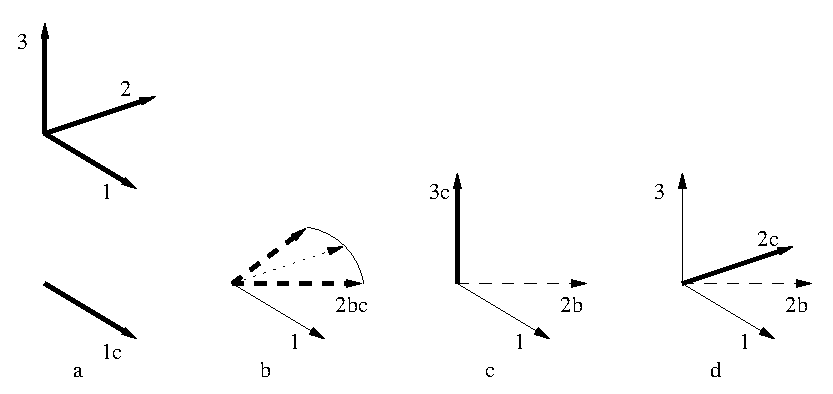
\includegraphics[width=.9\textwidth]{MatR2vec}
\caption{Construction of $3 \times 3$ orientation matrix from two
non-parallel vectors.}
\label{fig:general:orientation-matrices:MatR2vec}
\end{figure}

\subsection{($3 \times 3$) Orientation Matrix}
\label{sec:OrientationMatrix}
Implements the type \ty{OrientationMatrix}.
\begin{enumerate}
\item general case: two vectors that define an orthonormal reference
system, each of them preceded by its index in the final orientation matrix.
The procedure that builds the orientation matrix from the two vectors
is illustrated in Figure~\ref{fig:general:orientation-matrices:MatR2vec}.
\begin{Verbatim}[commandchars=\\\{\}]
    \bnt{v1} , \bnt{v1_1}, \bnt{v1_2} , \bnt{v1_3} ,
    \bnt{v2} , \bnt{v2_1}, \bnt{v2_2} , \bnt{v2_3}

    \bnt{v1} ::= \{ \kw{1} | \kw{2} | \kw{3} \}
    \bnt{v2} ::= \{ \kw{1} | \kw{2} | \kw{3} \} # \bnt{v2} != \bnt{v1}
\end{Verbatim}
The first vector, \bnt{v1}, namely vector 1 in subfigure (a), is normalized and assumed
to represent the desired direction.
The second vector, \bnt{v2}, namely vector 2' in subfigure (b), simply concurs
in the definition of the plane the vector that is not given is normal to.
The third vector, vector 3 in subfigure (c), results from the cross-product
of the first two vectors, after normalization.
The actual direction of the second vector, vector 2 in subfigure (d),
results from the cross product of the third and the first vector.

\noindent
\textbf{Examples.}
\begin{verbatim}
    1, 1.,0.,0., 2, 0.,1.,0.
\end{verbatim}
Equivalent to the identity matrix, i.e.\ no rotation 
occurs with respect to the initial reference frame: direction 1
in the final reference frame is parallel to \texttt{1.,0.,0.}, which represents
direction 1 in the initial reference frame, while direction 2 in the final reference frame
is parallel to \texttt{0.,1.,0.}, which represents direction 2
in the initial reference frame.
\begin{verbatim}
    1, cos(pi/6.), sin(pi/6.), 0.,
        3, 0.,0.,1.
\end{verbatim}
Rotation of $ \pi/6 $ radian about
initial direction 3: direction 1 in the final reference frame results from 
composing \kw{cos}\texttt{(pi/6.)} in initial direction 1
and \kw{sin}\texttt{(pi/6.)}
in initial direction 2, while direction 3 in the final reference frame remains
parallel to \texttt{0.,0.,1.}, which represents direction 3 in the initial reference frame.
\begin{verbatim}
    2, 0., cos(ALPHA), sin(ALPHA),
        1, 1.,0.,0.
\end{verbatim}
Rotation of \texttt{ALPHA} (assuming the variable \texttt{ALPHA} was previously defined) about
initial direction 1: direction 2 in the final reference frame results from 
composing \kw{cos}\texttt{(ALPHA)} in initial direction 2
and \kw{sin}\texttt{(ALPHA)}
in initial direction 2, while direction 3 in the final reference frame remains
parallel to \texttt{0.,0.,1.}, which represents direction 3 in the initial reference frame.

\item a variant of the above, which may be useful when only one
direction really matters, is
\begin{Verbatim}[commandchars=\\\{\}]
    \bnt{v1} , \bnt{v1_1}, \bnt{v1_2} , \bnt{v1_3} ,
    \bnt{v2} , \kw{guess}

    \bnt{v1} ::= \{ 1 | 2 | 3 \}
    \bnt{v2} ::= \{ 1 | 2 | 3 \} # \bnt{v2} != \bnt{v1}
\end{Verbatim}
and is illustrated in the example below:
\begin{verbatim}
    1, 1.,0.,0., 2, guess
\end{verbatim}
The keyword \kw{guess} tells the parser to generate a random vector
that is orthogonal to the given one, which is used as the direction
indicated by the index (2 in the example).
The vector is computed based on a very simple algorithm: it contains
\begin{itemize}
        \item 1.0 corresponding to the index with smallest modulus,
        $v_1\plbr{\mathrm{min}}$;
	\item $-v_1\plbr{\mathrm{min}}/v_1\plbr{\mathrm{max}}$
	corresponding to the index with the largest modulus,
	$v_1\plbr{\mathrm{max}}$;
	\item 0.0 for the remaining index.
\end{itemize}

\item identity matrix: keyword \kw{eye}; the identity matrix,
which means there is no rotation with respect to the global reference
frame.

\item a complete orientation matrix: keyword \kw{matr}
followed by the nine, row-oriented, coefficients, namely
$ r_{11} $, $ r_{12} $, \ldots, $ r_{33} $.
\begin{Verbatim}[commandchars=\\\{\}]
    \kw{matr} ,
        \bnt{r11} , \bnt{r12} , \bnt{r13} ,
        \bnt{r21} , \bnt{r22} , \bnt{r23} ,
        \bnt{r31} , \bnt{r32} , \bnt{r33}
            [ , \kw{tolerance} , \bnt{tol} ]
\end{Verbatim}
The \kw{tolerance} \nt{tol} is used when checking the orthogonality of the matrix (the default is $10^{-12}$).

\noindent
Example:
\begin{verbatim}
    matr,
        r11, r12, r13,
        r21, r22, r23,
        r31, r32, r33
\end{verbatim}
\emph{Note: orthogonality is not enforced; if the matrix is not orthogonal within the desired tolerance, only a warning is issued; be sure an orthogonal
matrix, within the desired tolerance, is input}.

\item Euler angles: keyword \kw{euler}, followed by the three
values, as output by structural nodes.
The keywords \kw{euler123} (same as \kw{euler}, also known as Tait-Bryan or Cardano angles), \kw{euler313} and \kw{euler321}
allow to use orientations in the sequence specified by the keyword.
\begin{Verbatim}[commandchars=\\\{\}]
    \{ \kw{euler} | \kw{euler123} | \kw{euler313} | \kw{euler321} \} ,
        [ \kw{degrees} , ]
        \bnt{angle_1} , \bnt{angle_2} , \bnt{angle_3}
\end{Verbatim}
\fbox{\begin{minipage}{.93\textwidth}%
Note: the output in the \texttt{.mov} file is in degrees,
while in input MBDyn requires angles in radians,
unless the values are preceded by the keyword \kw{degrees}.
\end{minipage}}

\emph{Note: the definition of the three angles that are used 
by the code to express orientations may vary between versions.
Currently, Bryant-Cardano angles are used in place of Euler
angles; see the note related to the output of the structural nodes
in Section~\ref{sec:NODE:STRUCTURAL:OUTPUT}, and the Technical Manual.
The code will remain consistent, i.e. the same angle
definition will be used for input and output, but models
over versions may become incompatible, so this syntax should 
really be used only as a means to quickly reproduce in the input
an orientation as resulting from a previous analysis.}

\item Orientation vector: keyword \kw{vector}, followed by the three
values, as output by structural nodes.
The resulting matrix is computed as
\begin{equation}
	\T{R} = \exp\plbr{\T{v}\times{}}
\end{equation}
\end{enumerate}

The keyword \kw{null} is intercepted, since its conventional usage
would result in a zero-valued matrix which, by definition, cannot be orthogonal;
an error is raised.

\subsection{$6 \times 6$ Matrix}
\label{sec:Mat6x6}
Implements the type \ty{Mat6x6}.
\begin{enumerate}
    \item general case: a sequence of 36 reals, comma-separated, that
    represent the row-oriented coefficients $ a_{11} $, $ a_{12}$ ,
    \ldots, $ a_{65} $, $ a_{66} $.
    \item ANBA format: keyword \kw{anba}, followed by 36 reals, 
    comma-separated, that represent the coefficients of the beam stiffness
    matrix as generated by the beam section analysis code ANBA,
    namely the following transformation is performed:
    \begin{itemize}
        \item axis $ x $, in the section plane in ANBA notation, 
	becomes axis 2 in MBDyn notation;    
	\item axis $ y $, in the section plane in ANBA notation, 
	becomes axis 3 in MBDyn notation;    
	\item axis $ z $, the beam axis in ANBA notation, 
	becomes axis 1 in MBDyn notation;    
    \end{itemize}
    \emph{Note: this format is mainly intended for backwards compatibility
    with older versions of that beam section analysis software,
    which used a different numbering convention for the reference frame
    that is local to the beam section.}
    \item symmetric matrix: keyword \kw{sym}, followed by a sequence
    of 21 reals, comma-separated, that represents the upper triangle,
    row-oriented coefficients of a symmetric matrix, 
    e.g. $ a_{11} $, \ldots , $ a_{16} $, $ a_{22} $,
    \ldots , $ a_{26} $, \ldots, $ a_{66} $.
    \item diagonal matrix: keyword \kw{diag}, followed by a sequence
    of 6 reals, comma-separated, that represent the diagonal coefficients 
    of a diagonal matrix.
    \item identity matrix: keyword \kw{eye}; the matrix is initialized
    as the identity matrix, that is a null matrix except for the diagonal 
    coefficients that are 1.
    \item null matrix: keyword \kw{null}; the matrix is initialized 
    with zeros.
\end{enumerate}
\subsection{$6 \times N$ Matrix}
\label{sec:Mat6xN}
Implements the type \ty{Mat6xN}.
\begin{enumerate}
    \item general case: a sequence of $6 \times N$ reals, comma-separated, that
    represent the row-oriented coefficients $ a_{11} $, $ a_{12}$ ,
    \ldots, $ a_{6\plbr{N-1}} $, $ a_{6N} $.
    \item ANBA format: keyword \kw{anba}, followed by $6 \times N$ reals,
    comma-separated, that represent the coefficients of the beam stiffness
    matrix as generated by the code ANBA, namely the following
    transformation is performed:
    \begin{itemize}
        \item axis $ x $, in the section plane in ANBA notation, 
	becomes axis 2 in MBDyn notation;    
	\item axis $ y $, in the section plane in ANBA notation, 
	becomes axis 3 in MBDyn notation;    
	\item axis $ z $, the beam axis in ANBA notation, 
	becomes axis 1 in MBDyn notation;    
    \end{itemize}
    \item null matrix: keyword \kw{null}; the matrix is initialized 
    with zeros.
\end{enumerate}

\subsection{$N \times 6$ Matrix}
\label{sec:MatNx6}
Implements the type \ty{MatNx6}.
\begin{enumerate}
    \item general case: a sequence of $N \times 6$ reals, comma-separated, that
    represent the row-oriented coefficients \\
    $ a_{11} $, $ a_{12}$ ,\ldots, $ a_{16}$,\\
    $ a_{21}$, $ a_{22}$, \ldots, $ a_{26}$,\\
    \ldots, \\
    $ a_{N1} $, $ a_{N2} $, \ldots, $ a_{N6}$.\\
    \item ANBA format: keyword \kw{anba}, followed by $N \times 6$ reals,
    comma-separated, with the columns representing the coefficients of the beam  
    generalized deformations as generated by the code ANBA, namely the following
    transformation is performed:
    \begin{itemize}
        \item axis $ x $, in the section plane in ANBA notation, 
	becomes axis 2 in MBDyn notation;    
	\item axis $ y $, in the section plane in ANBA notation, 
	becomes axis 3 in MBDyn notation;    
	\item axis $ z $, the beam axis in ANBA notation, 
	becomes axis 1 in MBDyn notation;    
    \end{itemize}
    \item null matrix: keyword \kw{null}; the matrix is initialized 
    with zeros.
\end{enumerate}

\subsection{$N \times N$ Matrix}
\label{sec:MatNxN}
Implements the type \ty{MatNxN}.
\begin{enumerate}
    \item general case: a sequence of $N \times 6$ reals, comma-separated, that
    represent the row-oriented coefficients $ a_{11} $, $ a_{12}$ ,
    \ldots, $ a_{N\plbr{N-1}} $, $ a_{NN} $.
    \item null matrix: keyword \kw{null}; the matrix is initialized 
    with zeros.
\end{enumerate}


\section{Input Related Cards} 
(Almost) everywhere in the input file the statement cards defined 
in the following can be used.
They are handled directly by the parsing object, and merely act as
an indirect reference to entities that are not explicitly enumerated.
They are:



\subsection{Constitutive Law}\label{sec:CONSTITUTIVE-LAW}
%\begin{verbatim}
\begin{Verbatim}[commandchars=\\\{\}]
    \bnt{card} ::= \kw{constitutive law} : \bnt{label} ,
        [ \kw{name} , " \bnt{name} " , ]
        \bnt{dim} , (\htmlref{\ty{ConstitutiveLaw}\be{\bnt{dim}\kw{D}}}{sec:ConstitutiveLaw}) \bnt{constitutive_law} ;
\end{Verbatim}
%\end{verbatim}
Constitutive laws are grouped by their dimensionality \nt{dim},
which (up to now) can be any of 1, 3, 6 and 7.
The \nt{constitutive\_law} is parsed according to the rules
described in Section~\ref{sec:ConstitutiveLaw},
and can be referenced later when it needs to be used.



\subsection{C81 Data}\label{sec:C81-DATA}
This keyword allows to define and read the \kw{c81 data} 
airfoil tables that are used by aerodynamic elements.
%\begin{verbatim}
\begin{Verbatim}[commandchars=\\\{\}]
    \bnt{card} ::= \kw{c81 data} : \bnt{label} [ , \kw{name} , " \bnt{name} " ]
        " \bnt{filename} "
        [ , \kw{tolerance} , \bnt{tolerance} ]
        [ , \{ \kw{free format} | \kw{nrel} | \kw{fc511} \} ]
        [ , \kw{flip} ]
        [ , \kw{echo} , " \bnt{output_filename} " [ , \kw{free format} ] ] ;
\end{Verbatim}
%\end{verbatim}
Data is read from file \nt{filename} according to the format specified
in the following.

The optional keyword \kw{tolerance} allows to specify the tolerance
that is used to determine the boundaries of the linear portion
of the lift curve slope.

The traditional format is used unless a format is specified using any
of the keywords \kw{free format}, \kw{nrel} or \kw{fc511}
(the latter is intentionally not documented).
The format is automatically inferred by reading the heading line
of the input file.

The optional keyword \kw{flip} instructs MBDyn to ``flip'' the data,
i.e.\ treat the airfoil data as if the sign of the angle of attack
changed along with that of the lift and moment coefficients,
but not that of the drag coefficient.
This corresponds to considering the airfoil ``upside down''.

The optional keyword \kw{echo} allows to specify the name of the file
that will be generated with the data just read, for cross-checking purposes.
If the following optional keyword is \kw{free format}, or if data was read
in free format, the echo will also be in free format.
Otherwise, it will be in the traditional format.

\subsubsection{Traditional Format}
The file is in textual form; the traditional format (the default) is:
\begin{itemize}
\item first line: \texttt{"\%30s\%2d\%2d\%2d\%2d\%2d\%2d"} 
where the first 30 chars are a title string, currently ignored by MBDyn,
followed by 6 consecutive two-digit integers that indicate:
	\begin{itemize}
	\item the number \texttt{ML} of \emph{Mach} points for $C_l$;
	\item the number \texttt{NL} of angle of attack points for $C_l$;
	\item the number \texttt{MD} of \emph{Mach} points for $C_d$;
	\item the number \texttt{ND} of angle of attack points for $C_d$;
	\item the number \texttt{MM} of \emph{Mach} points for $C_m$;
	\item the number \texttt{NM} of angle of attack points for $C_m$.
	\end{itemize}
The example in \texttt{var/naca0012.c81} contains:
{\small
\begin{verbatim}
1........01........01........0MLNLMDNDMMNM; not part of format
PROFILO NACA 0012             11391165 947
\end{verbatim}
}
\item the format of each following line is up to 10 fields of 7 chars each;
records longer than 10 fields are broken on multiple lines,
with the first field filled with blanks;
\item a block containing the $C_l$ data, made of:
	\begin{itemize}
	\item a record with the first field blank, followed by
	the \texttt{ML} \emph{Mach} values for the $C_l$;
	\item \texttt{NL} records containing the angle of attack
	in the first field, followed by \texttt{ML} values of $C_l$
	for each \emph{Mach} number; angles of attack wrap around 
	360 deg, starting from -180 deg.
	\end{itemize}
The example provided in file \texttt{var/naca0012.c81}
contains 11 \emph{Mach} points and 39 angle of attack records for the $C_l$
of the NACA0012 airfoil at high (unspecified) \emph{Reynolds}:
{\small
\begin{verbatim}
......7......7......7......7......7......7......7......7......7......7; not part of format
       0.     .20    .30    .40    .50    .60    .70    .75    .80
       .90    1.
-180.  0.     0.     0.     0.     0.     0.     0.     0.     0.
       0.     0.
-172.5 .78    .78    .78    .78    .78    .78    .78    .78    .78
       .78    .78
...
\end{verbatim}
}
\item a block containing the $C_d$ data, same as for $C_l$,
with \texttt{MD} \emph{Mach} points and \texttt{ND} angle of attack records;
\item a block containing the $C_m$ data, same as for $C_l$,
with \texttt{MM} \emph{Mach} points and \texttt{NM} angle of attack records.
\end{itemize}

\subsubsection{Free Format}
Finally, to allow higher precision whenever available, a native format,
based on \texttt{c81}, called \kw{free format}, is available.
It basically consists in the \texttt{c81} format without continuation lines
and with arbitrary precision, with fields separated by blanks.
The header is made of an arbitrary string, terminated by a semicolon `\texttt{;}',
followed by the six numbers that define the dimensionality of the expected data.

\paragraph{Example.} \
\begin{verbatim}
# FREE FORMAT
this is the header; 2 8 2 2 2 2
        0.0   0.9
-180.0  0.0   0.0
-170.0  1.0   0.9
 -90.0  0.0   0.0
 -10.0 -1.0  -0.9
  10.0  1.0   0.9
  90.0  0.0   0.0
 170.0 -1.0  -0.9
 180.0  0.0   0.0
        0.0   0.9
-180.0  0.1   0.1
 180.0  0.1   0.1
        0.0   0.9
-180.0  0.0   0.0
 180.0  0.0   0.0
\end{verbatim}

\subsubsection{NREL}
The \kw{nrel} format is used to provide airfoil data for wind turbines.
The format is very compact, but does not allow to account for Mach
dependence, and requires the same angle of attack resolution
for all three coefficients.
See AeroDyn's User Guide \cite{AERODYN-UG-2002} for a description
of the format.
Please note that MBDyn only supports one airfoil per file,
and only considers static coefficients from line 15 on.

\emph{To be completed.}

\subsubsection{Alternative Format}
An alternative format, required by some projects, can be used by supplying
the optional switch \kw{fc511}; it is intentionally not documented.

\subsubsection{Format Conversion}

Traditional format files can be automatically converted in free format
using the \texttt{c81test(1)} utility:
\begin{verbatim}
    $ c81test -d var/naca0012_free_format.c81 var/naca0012.c81
\end{verbatim}
generates a free format version of the NACA 0012 airfoil data
provided in the distribution.

\subsubsection{Miscellaneous}
A simple program that allows to read and plot the C81 tables
is available at \\
\htmladdnormallink{\texttt{http://homepage.mac.com/jhuwaldt/java/Applications/TableReader/TableReader.html}}
        {http://homepage.mac.com/jhuwaldt/java/Applications/TableReader/TableReader.html} \\
(thanks to Marco Fossati for pointing it out).

A simple utility that parses the C81 file and computes 
the aerodynamic coefficients for a given pair of angle of attack 
and Mach number is \texttt{c81test(1)}, available in the MBDyn utils suite.
This routine uses exactly the same code internally used by MBDyn,
so it should be considered a check of the code rather than a real tool.


\subsection{Drive Caller}\label{sec:DRIVE-CALLER}
The \kw{drive caller} directive
%\begin{verbatim}
\begin{Verbatim}[commandchars=\\\{\}]
    \bnt{card} ::= \kw{drive caller} : \bnt{label} ,
        [ \kw{name} , " \bnt{name} " , ]
        (\hty{DriveCaller}) \bnt{drive_caller} ;
\end{Verbatim}
%\end{verbatim}
allows to define
a \hyperref{\kw{drive caller}}{\kw{drive caller} (see Section~}{)}{sec:DriveCaller}
that can be subsequently reused.
It is useful essentially in two cases:
\begin{enumerate}
	\renewcommand{\labelenumi}{\alph{enumi})}
	\item to define a \htmlref{\kw{drive}}{sec:DriveCaller}
	that will be used many times throughout a model;
	\item to define a \htmlref{\kw{drive}}{sec:DriveCaller} 
	that needs to be used in a later defined part of a model, 
	in order to make it parametric.
\end{enumerate}



\subsection{Hydraulic fluid}\label{sec:HYDRAULIC-FLUID}
The \kw{hydraulic fluid} directive:
%\begin{verbatim}
\begin{Verbatim}[commandchars=\\\{\}]
    \bnt{card} ::= \kw{hydraulic fluid} : \bnt{label} , 
        \bnt{fluid_type} , \bnt{fluid_properties} ;
\end{Verbatim}
%\end{verbatim}
allows to define a hydraulic fluid to be later used in hydraulic elements,
see Section~\ref{sec:EL:HYDR}.
The fluid is identified by the \nt{label}. 
The \nt{fluid\_type}s, with the related \nt{fluid\_properties}, are
described in \ref{sec:HydraulicFluid}



\subsection{Include}\label{sec:INCLUDE}
The \kw{include} directive
%\begin{verbatim}
\begin{Verbatim}[commandchars=\\\{\}]
    \bnt{card} ::= \kw{include} : " \bnt{file_name} " ;
\end{Verbatim}
%\end{verbatim}
allows to include the contents of the file
\nt{file\_name},
which must be a valid filename for the operating system in
use.
The file name must be enclosed in double quotes (\texttt{"}).
The full (absolute or relative) path must be given if the included file 
is not in the directory of the including one.

\bigskip

\fbox{There is no check for recursively including files, so 
\textbf{the user must take care of avoiding recursions}.}

\bigskip

The \kw{include} directive forces the parser to scan the included file
\nt{file\_name} before continuing with the including one.
This is very useful if, for instance, a big model can be made of many
small models that are meaningful by themselves.

It can be used to replicate parts of the model, by simply using parametric 
labels for nodes, elements, reference systems, and setting a bias value 
before multiple-including the same bulk data file.
Examples of this usage are given in the tutorials
\htmladdnormallink{(\texttt{https://github.com/mmorandi/MBDyn-web/raw/main/userfiles/documents/tutorials.pdf})}
	{https://github.com/mmorandi/MBDyn-web/raw/main/userfiles/documents/tutorials.pdf} and examples
\htmladdnormallink{(\texttt{https://www.mbdyn.org/Documentation/Examples.html})}
	{https://www.mbdyn.org/Documentation/Examples.html}.



\subsection{Module Load}
\label{sec:GENERAL:MODULE-LOAD}
The \kw{module load} directive:
%\begin{verbatim}
\begin{Verbatim}[commandchars=\\\{\}]
    \bnt{card} ::= \kw{module load} : " \bnt{file_name} "
        [ , \bnt{module_arglist} ] ;

    \bnt{module_arglist} ::= \bnt{arg} [ , ... ]
\end{Verbatim}
%\end{verbatim}
where \nt{file\_name} is the name of a runtime loadable object,
causes the object to be opened, and a function \texttt{module\_init()},
with prototype
%\begin{verbatim}
\begin{Verbatim}[commandchars=\\\{\}]
        \textcolor{green}{extern} \textcolor{red}{"C"} \textcolor{green}{int}
        module_init(\textcolor{green}{const char} *module_name,
                \textcolor{green}{void} *data_manager, \textcolor{green}{void} *mbdyn_parser);
\end{Verbatim}
%\end{verbatim}
to be executed.

The function is assumed to perform the operations required to initialize
the module, eventually taking advantage of the parsing
and of the data manager; see the technical manual for details.

The function is also expected to take care of the optional \nt{module\_arglist}
arguments; in detail, module developers are encouraged to support
\kw{help} as the first optional argument.
The presence of this argument should result in printing to standard output
as much information as possible about the use of the module.

The typical use consists in registering some methods for later use.
A clear example is given in
\begin{verbatim}
        modules/module-wheel2/module-wheel2.cc
\end{verbatim}
where the \texttt{module\_init()} function registers
the \kw{user defined} element called \kw{wheel2}
in the set of user-defined element handlers.
The module can be retrieved later using the syntax described
in Section~\ref{sec:EL:BASE:USER_DEFINED}.
Note, however, that the \texttt{module\_init()} function may be used
for any purpose.
A typical use consists in registering any kind of handlers
for subsequent use.

Run-time module loading is taken care of by GNU's \texttt{libltdl}.
Modules are compiled using \texttt{libtool} for portability purposes.
The resulting modules take the name
\texttt{libmodule-<name>.la}.

Modules are installed by default in the directory
\texttt{\$\{prefix\}/libexec}.
When loaded using only the module name, the default directory is searched.
The run-time loading path can be modified by the 
\kw{loadable path} statement described
in Section~\ref{sec:CONTROLDATA:LOADABLE_PATH}.

Although \texttt{libltdl} is supposed to be portable on a wide variety
of platforms (this is what it is designed for, all in all),
run-time loading within MBDyn is mainly tested using Linux.
Users are encouraged to report problems they might encounter,
especially when building modules for different platforms,
as this would help making MBDyn more portable.



\subsection{Print symbol table}
The \kw{print symbol table} directive:
%\begin{verbatim}
\begin{Verbatim}[commandchars=\\\{\}]
    \bnt{card} ::= \kw{print symbol table} [ : { \kw{all} | \bnt{namespace_list} } ] ;

    \bnt{namespace_list} ::= \bnt{namespace} [ , \bnt{namespace_list} ]
\end{Verbatim}
%\end{verbatim}
allows to print to standard output the contents of the parser's symbol
table at any stage of the input phase.
This may be useful for model debugging purposes.

When no arguments are provided, it prints the symbol table of the math parser.
Otherwise, it prints the symbol table associated with a specific namespace,
according to the list of arguments (all namespaces when the keyword \kw{all} is used).



\subsection{Reference}
The \kw{reference} directive:
%\begin{verbatim}
\begin{Verbatim}[commandchars=\\\{\}]
    \bnt{card} ::= \kw{reference} : \bnt{unique_label} , 
        [ \kw{name} , (\ty{string}) \bnt{name} , ]
        [ \kw{position} , ]         (\hty{Vec3}) \bnt{absolute_position} ,
        [ \kw{orientation} , ]      (\hty{OrientationMatrix}) \bnt{absolute_orientation_matrix} ,
        [ \kw{velocity} , ]         (\hty{Vec3}) \bnt{absolute_velocity} ,
        [ \kw{angular velocity} , ] (\hty{Vec3}) \bnt{absolute_angular_velocity} ;
\end{Verbatim}
%\end{verbatim}
A \kw{reference} system is declared and defined.
It must be given a unique identifier, scanned by the math parser
(which means that any regular expression is allowed, and the result is
rounded up to the nearest unsigned integer).
The entries \nt{absolute\_*} are parsed by routines that
compute absolute (i.e.\ referring to the global frame) entities
starting from a given entity in a given reference frame.
These routines are very general, and make intense use of the 
\kw{reference} entries themselves, which means that a reference 
can be recursively defined by means of previously defined 
\kw{reference} entries.

\bigskip

Alternative form, based on Denavit-Hartenberg parameters,
which are particularly used in robotics.
It defines the reference system of the second part of a joint with respect to the first part,
when the two parts are connected by revolute joints.
%\begin{verbatim}
\begin{Verbatim}[commandchars=\\\{\}]
    \bnt{card} ::= \kw{reference} : \bnt{unique_label} , 
        [ \kw{name} , " \bnt{name} " , ]
        \kw{Denavit Hartenberg} ,
        [ \kw{reference} , \{ \kw{global} | \bnt{ref_label} \} , ]
        \bnt{d} , \bnt{theta} , \bnt{a} , \bnt{alpha} ;
\end{Verbatim}
%\end{verbatim}
where:
\begin{itemize}
\item \nt{d}: offset $d$ along previous $z$ axis to the common normal (the current $x$ axis);

\item \nt{theta}: the angle $\theta$ about previous $z$ from previous to current $x$ axis;

\item \nt{a}: length $a$ of the common normal; for revolute joints, the radius of the previous $z$;

\item \nt{alpha}: the angle $\alpha$ about the common normal, from previous to new $z$ axis.
\end{itemize}
The configuration of the first part of the joint is identified by an axis $z_1$ and a point $\text{P}_1$ on it.
The configuration of the second part of the joint is identified by an axis $z_2$;
point $\text{P}_2$ on the second part of the joint results from the definition itself,
and is not strictly relevant for the definition.
If the two axes are not parallel, they have a common normal, $x_2$, that crosses both;
otherwise, one can arbitrarily choose $x_2$ as a direction orthogonal to both $z_1$
(and $z_2$, since they are parallel, or even coincident).
Choose $x_1$ as a vector normal to $z_1$, originating from the reference point of the first part of the joint, $\text{P}_1$,
and directed towards the reference point of the second part of the joint, $\text{P}_2$
(this is not strictly required, as one can choose axis $x_1$ at will, as it only provides the reference for the joint rotation).
In general, $x_1$ will not be able to intersect axis $z_2$, unless axes $z_1$ and $z_2$ are co-planar.
Point $\text{P}_2$ is the intersection between axes $x_2$ and $z_2$.
If needed, axes $y_1$ and $y_2$ are defined according to the right-hand rule.
Then:
\begin{itemize}
\item \nt{d} is the distance, along $z_1$, between the reference point of the first part, $\text{P}_1$, and the plane determined by axes $z_2$ and $x_2$;

\item \nt{theta} is the angle about axis $z_1$ between axes $x_2$ and $x_1$; it represents the actual rotation of the joint;

\item \nt{a} is the distance between axes $z_1$ and $z_2$, which is along axis $x_2$;

\item \nt{alpha} is the angle formed by axis $z_2$ with respect to axis $z_1$; it corresponds to a rotation about axis $x_2$.
\end{itemize}

The new reference data are
\begin{subequations}
\begin{align}
	\T{x}_\text{new}
	&=
	\T{x}_\text{old}
	+
	\TT{R}_\text{old} \plbr{
		\nt{d} \, \T{e}_3
		+
		\text{exp}\plbr{\plbr{\nt{theta} \, \T{e}_3} \times{}} \cdot \plbr{\nt{a} \, \T{e}_1}
	}
	\\
	\TT{R}_\text{new}
	&=
	\TT{R}_\text{old} \text{exp}\plbr{\plbr{\nt{theta} \, \T{e}_3} \times{}} \text{exp}\plbr{\plbr{\nt{alpha} \, \T{e}_1} \times{}}
	\\
	\T{v}_\text{new}
	&=
	\T{v}_\text{old}
	+
	\T{\omega}_\text{old} \times \TT{R}_\text{old} \plbr{
		\nt{d} \, \T{e}_3
		+
		\text{exp}\plbr{\plbr{\nt{theta} \, \T{e}_3} \times{}} \cdot \plbr{\nt{a} \, \T{e}_1}
	}
	\\
	\T{\omega}_\text{new}
	&=
	\T{\omega}_\text{old}
\end{align}
\end{subequations}
where the subscript ``old'' refers to the reference frame with label \nt{ref\_label1}, if any, or otherwise to the global reference system.

\subsubsection{Use of Reference Frames}
Every time an absolute or a relative geometric or physical entity is
required, it is processed by a set of routines that allow the entity to be
expressed in the desired reference frame.
The following cases are considered:
\begin{itemize}
    \item relative position (physical)
    \item absolute position (physical)
    \item relative orientation matrix (physical)
    \item absolute orientation matrix (physical)
    \item relative velocity (physical)
    \item absolute velocity (physical)
    \item relative angular velocity (physical)
    \item absolute angular velocity (physical)
    \item relative arbitrary vector (geometric)
    \item absolute arbitrary vector (geometric)    
\end{itemize}
The caller is responsible for the final interpretation of the input. 
The caller always supplies the routines a default reference structure
the input must be referred to.
So, depending on the caller, the entry can be in the following forms:
\begin{enumerate}
\item \bnt{entity}: \\ 
	the data supplied in \nt{entity} is intended 
	in the default reference frame
\item \texttt{\kw{reference} , \bnt{reference\_type} , \bnt{entity}}: \\
	the data are in \nt{reference\_type} reference frame, where
%\begin{verbatim}
\begin{Verbatim}[commandchars=\\\{\}]
        \bnt{reference_type} ::= \{ \kw{global} | \kw{node} | \kw{local} \}
\end{Verbatim}
%\end{verbatim}
\item \texttt{\kw{reference} , \bnt{reference\_label} , \bnt{entity}}: \\
	the data are in \nt{reference\_label} reference frame. 
	This reference frame must be already defined. 
\end{enumerate}
In some cases, significantly in case of joints (see Section~\ref{sec:EL:JOINT}) that connect two nodes
$a$ and $b$, special reference types are allowed
when reading specific entities related to the second node.
These reference types compute the value of the entity with respect
to the reference frame associated with the first node, $a$:
\begin{enumerate}
\item \kw{other position}: \\
	a relative position $\tilde{\T{p}}$ is intended in the other node's
	reference frame, with respect to the relative position $\tilde{\T{f}}_a$
	already specified for the other node,
\begin{equation}
	\tilde{\T{f}}_b = \TT{R}_b^T\plbr{
		\T{x}_a + \TT{R}_a \plbr{
			\tilde{\T{f}}_a
			+ \tilde{\T{p}}
		}
		- \T{x}_b
	} ,
\end{equation}
	which is the solution of equation
\begin{equation}
	\T{x}_a + \TT{R}_a \plbr{\tilde{\T{f}}_a + \tilde{\T{p}}}
	= \T{x}_b + \TT{R}_b \tilde{\T{f}}_b ;
\end{equation}

\item \kw{other orientation}: \\
	a relative orientation $\tilde{\TT{R}} $ is intended in the other node's
	reference frame, with respect to the relative orientation
	$\tilde{\TT{R}}_{ha}$ already specified for the other node,
\begin{equation}
	\tilde{\TT{R}}_{hb} = \TT{R}_b^T \TT{R}_a \tilde{\TT{R}}_{ha} \tilde{\TT{R}} ,
\end{equation}
	which is the solution of equation
\begin{equation}
	\TT{R}_a \tilde{\TT{R}}_{ha} \tilde{\TT{R}}
	= \TT{R}_b \tilde{\TT{R}}_{hb} ;
\end{equation}

\item \kw{other node}: \\
	a relative position $\tilde{\T{p}}$
	or a relative orientation $\tilde{\TT{R}}$
	are intended in the other node's reference frame,
\begin{subequations}
\begin{align}
	\tilde{\T{f}}_b &= \TT{R}_b^T\plbr{
		\T{x}_a + \TT{R}_a \tilde{\T{p}}
		- \T{x}_b
	} \\
	\tilde{\TT{R}}_{hb} &= \TT{R}_b^T \TT{R}_a \tilde{\TT{R}} ,
\end{align}
\end{subequations}
	which are the solutions of equations
\begin{subequations}
\begin{align}
	\T{x}_a + \TT{R}_a \tilde{\T{p}}
	&= \T{x}_b + \TT{R}_b \tilde{\T{f}}_b \\
	\TT{R}_a \tilde{\TT{R}}
	&= \TT{R}_b \tilde{\TT{R}}_{hb} .
\end{align}
\end{subequations}
\end{enumerate}

\paragraph{Example.} \
\begin{itemize}
    \item absolute position:
    \begin{verbatim}
    null
    reference, global, null
    reference, 8, 1., sin(.3*pi), log(3.)
    \end{verbatim}
    \item relative orientation matrix (e.g.\ as required by many constraints and
    thus referred to a node):
    \begin{verbatim}
    eye
    reference, node, eye
    reference, 8,
        3, 0., 1., 0., 
        1, .5, sqrt(3)/2., 0.
    \end{verbatim}
\end{itemize}
Notes: 
\begin{itemize}
    \item the global reference frame has position $ \cubr{0, 0, 0} $,
    orientation matrix \kw{eye}, velocity $ \cubr{0, 0, 0} $ and angular
    velocity $ \cubr{0, 0, 0} $.
    \item if the caller is not related to a node, the reference type
    \kw{node} is not defined. 
    % In this case it is considered equivalent to \kw{local}.
    \item when processing a velocity or an angular velocity, the resulting
    value always accounts for the velocity and angular velocity of the frame
    the entry is referred to. 

    As an example, if a node is defined in a reference frame $\T{R}_R$
    that has non-null angular velocity $ \T{\Omega}_R $, and the position 
    $ \T{x}_{\text{input}} $ of the node is not coincident
    with the origin $ \T{X}_R $ of the reference frame
    it is attached to, its global velocity and angular velocity result
    as the composition of the input values and of those of the reference 
    frame:
    \begin{eqnarray*}    
        \T{w} & = & \T{R}_R \T{\omega}_{\text{input}} + \T{\Omega}_R \\
	\T{v} & = & \T{R}_R \T{v}_{\text{input}} + \T{V}_R
		+\T{\Omega}_R\times\plbr{\T{R}_R \T{x}_{\text{input}}}
    \end{eqnarray*}
    This, for instance, eases the input of all the parts of a complex system
    that is moving as a rigid body, by defining a reference frame with the
    proper initial linear and angular velocity, and then referring all the entities, e.g.\ the 
    nodes, to that frame, with null local linear and angular velocity.
\end{itemize}  
{\em
    Recalling the declaration and the definition of reference frames,
    a simple reference frame definition, with all the entries referring 
    by default to the global system, would be:
    \begin{verbatim}
    reference: 1000,
        null,
        eye,
        null,
        null;
    \end{verbatim}
    which represents a redefinition of the global system.

    A more verbose, and self-explanatory definition would be:
    \begin{verbatim}
    reference: 1000,
        reference, global, null,
        reference, global, eye,
        reference, global, null,
        reference, global, null;			 
    \end{verbatim}
    The reference frame one is referring to must be repeated for all the entries
    since they must be allowed to refer to whatever frame is preferred 
    by the user.

    A fancier definition would be:
    \begin{verbatim}
    reference: Rotating_structure, 
        reference, Fixed_structure, null,
        reference, Spindle_1,
            1, 0., 0., 1., 
            3, 0., 1., 0.,
        reference, Fixed_structure, null,
        reference, Spindle_1, 0., 0., Omega_1;
    \end{verbatim}
}

\subsubsection{Output}
The reference frames are used only during the input phase, 
where they help referring entities either absolute 
or relative to other entities depending on their internal representation
during the analysis.
As such, reference frames cannot be ``used'' or ``visualized'' neither 
directly nor indirectly at any time during the analysis or by interpreting
the output, because they do not ``evolve'' nor are attached
to any state-dependent entity.
To allow their debugging, however, they can be output in the global
reference frame according to the representation of structural nodes,
as described in Section~\ref{sec:NODE:STRUCTURAL:OUTPUT}, 
by using the \kw{default output} directive 
with the value \kw{reference frames}, as detailed
in Section~\ref{sec:CONTROLDATA:DEFAULTOUTPUT}.



\subsection{Remark}
The \kw{remark} directive:
%\begin{verbatim}
\begin{Verbatim}[commandchars=\\\{\}]
    \bnt{card} ::= \kw{remark} [ : \bnt{math_expression} [ , ... ] ] ;
\end{Verbatim}
%\end{verbatim}
This directive simply prints to stdout the (list of) expression(s) \nt{math\_expression}.
It is used to allow rough input debugging. The file name and line number
are logged first, followed by the result of the evaluation of the expression(s list). 

\paragraph{Example.} \
A file ``remarks'', containing only the statements
\begin{verbatim}
    remark: "square root of 2", sqrt(2);
    set: (
        real EA = 1e6; # N, axial stiffness
        real GA = 1e6; # N, shear stiffness
        real EJ = 1e3; # Nm^2, bending stiffness
        real GJ = 1e3; # Nm^2, torsional stiffness
    0);
    remark: "Stiffness properties", EA, GA, EJ, GJ;
\end{verbatim}
results in
\begin{verbatim}
user@host:~>$ mbdyn -f remarks

MBDyn - Multi-Body Dynamics 1.6.2
configured on Jun 26 2015 at 10:17:02

Copyright 1996-2023 (C) Paolo Mantegazza and Pierangelo Masarati,
Dipartimento di Ingegneria Aerospaziale <http://www.aero.polimi.it/>
Politecnico di Milano                   <http://www.polimi.it/>

MBDyn is free software, covered by the GNU General Public License,
and you are welcome to change it and/or distribute copies of it
under certain conditions.  Use 'mbdyn --license' to see the conditions.
There is absolutely no warranty for MBDyn.  Use "mbdyn --warranty"
for details.

reading from file "remarks"
line 1, file <remarks>: square root of 2, 1.41421
line 8, file <remarks>: Stiffness properties, 1e+06, 1e+06, 1000, 1000
MBDyn terminated normally
user@host:~>$
\end{verbatim}
Notice that in the example above the first expression is actually a string,
as it was required up to version 1.6.1; this is no longer required.

\subsection{Set}
The \kw{set} directive:
%\begin{verbatim}
\begin{Verbatim}[commandchars=\\\{\}]
    \bnt{card} ::= \kw{set} : \bnt{math_expression} ;
\end{Verbatim}
%\end{verbatim}
This directive simply invokes the math parser to evaluate the expression
\nt{math\_expression} and then discards the result.

It can be used to declare new variables, or to set the values
of existing ones.
This feature is very useful, since it allows to build parametric models,
and to reuse generic model components.

\paragraph{Example.} \
\begin{verbatim}
    set: integer LABEL = 1000;    # a label
    set: real E = 210e+9;         # Pa, steel's elastic module
    set: real A = 1e-4;           # m^2, a beam's cross section
    set: real K = E*A;            # N, a beam's axial stiffness
\end{verbatim}



\subsection{Setenv}
The \kw{setenv} directive:
%\begin{verbatim}
\begin{Verbatim}[commandchars=\\\{\}]
    \bnt{card} ::= \kw{setenv} :
        [ \kw{overwrite} , \{ \kw{yes} | \kw{no} | (\ty{bool}) \bnt{overwrite} \} , ]
        " \bnt{varname} [ = \bnt{value} ] " ;
\end{Verbatim}
%\end{verbatim}
This directive sets the environment variable \nt{varname} 
to \nt{value}, if given; otherwise, the variable
is unset.
If \kw{overwrite} is set, the variable is overwritten, 
if already set.
By default, \kw{overwrite} is set according to \texttt{setenv(3)}'s
overwrite parameter (\kw{no}).
\begin{verbatim}
    # set FILE to "test", if it does not exist
    setenv: "FILE=test";
    # set FILE to "test", even if it exists
    setenv: overwrite, yes, "FILE=test";
    # unset FILE
    setenv: "FILE";
    # set FILE to the empty string, if it does not exist
    setenv: "FILE=";
\end{verbatim}
See \texttt{setenv(3)} and \texttt{unsetenv(3)}
(or \texttt{putenv(3)}, if the former is not available)
man pages for details.




\subsection{Template Drive Caller}\label{sec:TPL-DRIVE-CALLER}
The \kw{template drive caller} directive
%\begin{verbatim}
\begin{Verbatim}[commandchars=\\\{\}]
    \bnt{card} ::= \kw{template drive caller} : \bnt{label} , \{ " \bnt{dim_name} " | (\ty{integer}) \bnt{dim} \} ,
        (\htybent{TplDriveCaller}{Entity}) \bnt{tpl_drive_caller} ;

    \bnt{dim_name} ::= \{ \kw{1} | \kw{3} | \kw{6} | \kw{3x3} | \kw{6x6} \}

    \bnt{dim} ::= \{ \kw{1} | \kw{3} | \kw{6} \}
\end{Verbatim}
%\end{verbatim}
allows to define
a \hyperref{\kw{template drive caller}}{\kw{template drive caller} (see Section~}{)}{sec:TplDriveCaller}
that can be subsequently reused.
The type is defined according to
\begin{center}
\begin{tabular}{lcc}
\hline
\ty{Entity} & \nt{dim\_name} & \nt{dim} \\
\hline
\ty{real}	& \kw{1} & \kw{1} \\
\hty{Vec3}	& \kw{3} & \kw{3} \\
\hty{Vec6}	& \kw{6} & \kw{6} \\
\hty{Mat3x3}	& \kw{3x3} & \\
\hty{Mat6x6}	& \kw{6x6} & \\
\hline
\end{tabular}
\end{center}
Template drive callers are useful essentially in two cases:
\begin{enumerate}
	\renewcommand{\labelenumi}{\alph{enumi})}
	\item to define a \htmlref{\kw{template drive}}{sec:TplDriveCaller}
	that will be used many times throughout a model;
	\item to define a \htmlref{\kw{template drive}}{sec:TplDriveCaller} 
	that needs to be used in part of a model that is defined later, 
	in order to make it parametric.
\end{enumerate}






\section{Node Degrees of Freedom}\label{sec:NodeDof}
A node in MBDyn is an entity that owns public degrees of freedom
and instantiates the corresponding public equations.
It can lend them to other entities, called elements, to let them write
contributions to public equations, possibly depending on the value
of the public degrees of freedom. 

Usually elements access nodal degrees of freedom through well-defined
interfaces, at a high level. 
But in a few cases, nodal degrees of freedom must be accessed
at a very low level, with the bare knowledge of the node label,
the node type, the internal number of the degree of freedom,
and the order of that degree of freedom (algebraic or differential, if any).
The data that allows an entity to track a nodal degree of freedom
is called \hty{NodeDof}; it is read according to
%\begin{verbatim}
\begin{Verbatim}[commandchars=\\\{\}]
    \bnt{node_dof} :: = \bnt{node_label} , 
        \bnt{node_type}
        [ , \bnt{dof_number} ]
        [ , \{ \kw{algebraic} | \kw{differential} \} ]
\end{Verbatim}
%\end{verbatim}
The label \nt{node\_label} and the type \nt{node\_type}
of the node are used to track the pointer to the desired node. 

If \nt{node\_type} refers to a non-scalar node type,
the \nt{dof\_number} field is required to indicate the requested
degree of freedom.

Finally, the order of the degree of freedom is read, if required.
It must be one of \kw{algebraic} or \kw{differential}.
If the \nt{dof\_number} degree of freedom is differential, both
orders can be addressed, while in case of a node referring
to an algebraic degree of freedom there is no choice,
only the \nt{algebraic} order can be addressed and thus this field
is not required.

The \nt{dof\_number} must be between 1 and the number of degrees of freedom
related to the node.
Not all numbers might be valid for specific nodes; for example,
\nt{dof\_number} values 4, 5, and 6 are not valid for a
\hyperref{\kw{structural node}}{\kw{structural node}, Section~}{}{sec:NODE:STRUCTURAL} when the order is \kw{algebraic}.

When the node degree of freedom input syntax is used to address
an equation (as in
\hyperref{\kw{abstract} force elements}{\kw{abstract} force elements, Section~}{}{sec:EL:FORCE:ABSTRACT},
or in
\hyperref{\kw{discrete control} elements}{\kw{discrete control} elements, Section~}{}{sec:EL:DISCCTRL}),
the distinction between \kw{algebraic} and \kw{differential} is meaningless,
and thus this field is not required.




\section{Drives and Drive Callers}\label{sec:DriveCaller}
Implements the type \hty{DriveCaller}.
Every time some entity can be ``driven'', i.e.\ a value can be
expressed as dependent on some ``external'' input, an object of the class 
\hty{DriveCaller} is used. 
The \kw{drive} essentially represents a scalar function, whose
value can change over time or, through some more sophisticated
means, can depend on the state of the analysis.
Usually, the dependence over time is implicitly assumed, unless
otherwise specified.
For example, the amplitude of the force applied by a 
\hyperref{\kw{force} element}{\kw{force} element (see Section~}{)}{sec:EL:FORCE}
is defined by means of a \kw{drive}; as such, the value of the \kw{drive} 
is implicitly calculated as a function of the time.
However, a 
\hyperref{\kw{dof drive}}{\kw{dof drive} (see Section~}{)}{sec:DriveCaller:DOF}
uses a subordinate \kw{drive} to compute its value based on the value
of a degree of freedom of the analysis; as a consequence,
the value of the \kw{dof drive} is represented by the
value of the subordinate \kw{drive} when evaluated as a function
of that specific degree of freedom at the desired time (function of function).

The family of the \hty{DriveCaller} object is very large.
The type of the \hty{DriveCaller} is declared as
%\begin{verbatim}
\begin{Verbatim}[commandchars=\\\{\}]
    \bnt{drive_caller} ::=
        \{ \bnt{drive_caller_type} [ , \bnt{arglist} ]
            | \kw{reference} , \bnt{label} \}
\end{Verbatim}    
%\end{verbatim}    
where \nt{arglist}, if any, is a comma-separated list of arguments
that depends on \nt{drive\_caller\_type}.
As an exception, a constant \hty{DriveCaller} (that behaves exactly as a
numerical constant with little or no overhead depending on the optimizing
capability of the compiler) is assumed when a numeric value is used instead
of a keyword.

If the alternative format is used, the keyword \kw{reference} 
must be followed by the label of an already defined, valid drive caller
(See Section~\ref{sec:DRIVE-CALLER}).

Drive callers are listed in Table~\ref{tab:DRIVE:DRIVE-CALLERS}.

\begin{table}
\centering
\caption{Drive callers}
\label{tab:DRIVE:DRIVE-CALLERS}
\begin{tabular}{lcl}
\hline
\textbf{Name} & \textbf{Differentiable} & \textbf{Notes} \\
\hline\hline
\kw{array} & $\surd$ & depends on subordinate drive callers \\
\kw{bistop} & & \\ %
\kw{closest next} & $\surd$ & depends on subordinate drive caller \\
\kw{const} & $\surd$ & \\
\kw{cosine} & $\surd$ & \\
\kw{cubic} & $\surd$ & \\
\kw{direct} & $\surd$ & \\ %
\kw{discrete filter} & & \\ %
\kw{dof} & & depends on subordinate drive caller \\ %
\kw{double ramp} & $\surd$ & \\
\kw{double step} & $\surd$ & \\
\kw{drive} & $\surd$ & depends on subordinate drive callers \\ %
\kw{element} & $\surd$ & depends on subordinate drive caller \\ %
\kw{exponential} & $\surd$ & \\
\kw{ginac} & $\surd$ & symbolic differentiation using GiNaC \\
\kw{file} & & \\ %
\kw{fourier series} & $\surd$ & \\
\kw{frequency sweep} & $\surd$ & depends on subordinate drive callers \\
\kw{linear} & $\surd$ & \\
\kw{meter} & $\surd$ & \\ %
\kw{mult} & $\surd$ & depends on subordinate drive callers \\ %
\kw{node} & $\surd$ & depends on subordinate drive caller \\ %
\kw{null} & $\surd$ & \\
%\kw{one} & $\surd$ & \\
\kw{parabolic} & $\surd$ & \\
\kw{periodic} & $\surd$ & depends on subordinate drive caller \\
\kw{piecewise linear} & $\surd$ & \\
\kw{ramp} & $\surd$ & \\
\kw{random} & $\surd$ & \\ %
\kw{sample and hold} & & \\ %
\kw{scalar function} & $\surd$ & depends on underlying scalar function \\
\kw{sine} & $\surd$ & \\
\kw{step} & $\surd$ & \\
\kw{step5} & $\surd$ & \\
\kw{string} & $\surd$ & \\ %
\kw{tanh} & $\surd$ & \\
\kw{time} & $\surd$ & \\
\kw{timestep} & $\surd$ & \\
\kw{unit} & $\surd$ & \\ %
\hline
\end{tabular}
\end{table}

\subsection{Array drive}
%\begin{verbatim}
\begin{Verbatim}[commandchars=\\\{\}]
    \bnt{drive_caller} ::= \kw{array} ,
        \bnt{num_drives} ,
            (\hty{DriveCaller}) \bnt{drive_caller}
            [ , ... ]
\end{Verbatim}
%\end{verbatim}
this is simply a front-end for the linear combination of \nt{num\_drives} 
normal drives; \nt{num\_drives} must be at least 1, in which case 
a simple drive caller is created, otherwise an array of drive callers 
is created and at every call their value is added to give 
the final value of the array drive.

\subsection{Bistop drive}
%\begin{verbatim}
\begin{Verbatim}[commandchars=\\\{\}]
    \bnt{drive_caller} ::= \kw{bistop} ,
        [ \kw{initial status}, \{ \kw{active} | \kw{inactive} \} , ]
            (\hty{DriveCaller}) \bnt{activation_condition} ,
            (\hty{DriveCaller}) \bnt{deactivation_condition}
\end{Verbatim}
%\end{verbatim}
This drive caller returns 1.0 (\kw{TRUE}) when its status is \kw{active} and 0.0 (\kw{FALSE}) when it is \kw{inactive}.
When in \kw{inactive} status, it turns to \kw{active} if the \nt{activation\_condition} is \kw{TRUE}.
When in \kw{active} status, it turns to \kw{inactive} if the \nt{deactivation\_condition} is \kw{TRUE}.

This drive caller is useful to implement a ``robust'' and irreversible status change, for example the deactivation of something, as
\begin{verbatim}
    bistop,
        initial status, active,
        # never re-activate
        null,
        # deactivate when the vertical component of node 1 velocity becomes negative
        string, "model::node::structural(1, \"XP[3]\") < 0"
\end{verbatim}

\subsection{Closest next drive}
\label{sec:DriveCaller:CLOSEST_NEXT}
%\begin{verbatim}
\begin{Verbatim}[commandchars=\\\{\}]
    \bnt{drive_caller} ::= \kw{closest next} ,
        \bnt{initial_time} ,
        \{ \kw{forever} | \bnt{final_time} \} ,
        (\hty{DriveCaller}) \bnt{increment}
\end{Verbatim}
%\end{verbatim}
This drive returns a non-zero value when called for the first time
with an argument greater that or equal to the current threshold value,
which is computed starting from \nt{initial\_time} and incrementing
it each time by as many \nt{increment} values as required to pass
the current value of \kw{Time}.
As soon as a threshold value is exceeded, as many values of \nt{increment}
as required to pass the current value of \kw{Time} are added,
and the process repeats.

This drive caller is useful within the \kw{output meter} statement
(see Section~\ref{sec:CONTROLDATA:OUTPUTMETER})
to obtain nearly equally spaced output when integrating
with variable time step.

\subsection{Const(ant) drive}
%\begin{verbatim}
\begin{Verbatim}[commandchars=\\\{\}]
    \bnt{drive_caller} ::= [ \kw{const} , ] \bnt{const_coef}
\end{Verbatim}
%\end{verbatim}
The keyword \kw{const} can be omitted, thus highlighting the real nature
of this driver, that is completely equivalent to a constant, static real
value.

\subsection{Cosine drive}
%\begin{verbatim}
\begin{Verbatim}[commandchars=\\\{\}]
    \bnt{drive_caller} ::= \kw{cosine} ,
        \bnt{initial_time} ,
        \bnt{angular_velocity} ,
        \bnt{amplitude} ,
        \{ [ - ] \bnt{number_of_cycles} | \kw{half} | \kw{one} | \kw{forever} \} , 
        \bnt{initial_value}
\end{Verbatim}
%\end{verbatim}
where \nt{angular\_velocity} is $2\pi/T$.
This drive actually computes a function of the type
\begin{align}
	f\plbr{t} &= \nt{initial\_value} + \nt{amplitude} \cdot \plbr{
		1 - \llk{cos}\plbr{
			\nt{angular\_velocity} \cdot \plbr{
				t - \nt{initial\_time}
			}
		}
	} .
\end{align}
The value of \nt{number\_of\_cycles} determines the behavior of the
drive. 
If it is positive, \nt{number\_of\_cycles} oscillations are performed.
If it is negative, the oscillations end after
\nt{number\_of\_cycles}$-1/2$ cycles at the top of the cosine, with null
tangent.   
Special keywords can be used for \nt{number\_of\_cycles}:
\begin{itemize}
	\item \kw{forever}: the oscillation never stops;
	\item \kw{one}: exactly one cycle is performed (equivalent to \nt{number\_of\_cycles} = 1);
	\item \kw{half}: exactly half cycle is performed (equivalent to \nt{number\_of\_cycles} = -1),
	so the function stops at
	\begin{align}
		f &= \nt{initial\_value} \nonumber \\
		& \mbox{} + \lcubr{\matr{ll}{
			0 & \text{when } t \le \nt{initial\_time}
			\\ \\
			\multicolumn{2}{l}{\nt{amplitude} \cdot ( 1 - \cos( \nt{angular\_velocity} \cdot (t - \nt{initial\_time})))}
			\\
				& \text{when } \nt{initial\_time} < t < \nt{initial\_time} + \cfrac{\pi}{\nt{angular\_velocity}}
			\\
			2 \cdot \nt{amplitude} & \text{when } \nt{initial\_time} + \cfrac{\pi}{\nt{angular\_velocity}} \le t
		}}
	\end{align}
	starting and ending with continuous first derivative.
	In this case, it may be convenient to indicate the \nt{angular\_velocity}
	as $\pi/\nt{duration}$, where \nt{duration} is the time
	required to complete the half-wave.
\end{itemize}
Note that this drive caller \underline{does not correspond to} $\cos(t)$. 

\paragraph{Example.}
\begin{verbatim}
    # starts at Time = 1.5, duration = T, amplitude = A, a "bump" of height 2*A
    ..., cosine, 1.5, 2*pi/T, A, one, 0., ...

    # starts at Time = .5, duration = T, amplitude = A, half "bump", remains at 2*A
    ..., cosine, .5, pi/T, A, half, 0., ...

    # starts at Time = 1.2, frequency = Omega, amplitude = A, lasts forever
    ..., cosine, 1.2, Omega, A, forever, 0., ...
\end{verbatim}

\textbf{TODO: add a plot that exemplifies the three cases.}

\subsection{Cubic drive}
%\begin{verbatim}
\begin{Verbatim}[commandchars=\\\{\}]
    \bnt{drive_caller} ::= \kw{cubic} ,
        \bnt{const_coef} , 
        \bnt{linear_coef} ,
        \bnt{parabolic_coef} , 
        \bnt{cubic_coef}
\end{Verbatim}
%\end{verbatim}
The function
\begin{align}
	f\plbr{t} &= \nt{const\_coef} \nonumber \\
		&+ \nt{linear\_coef} \cdot t \nonumber \\
		&+ \nt{parabolic\_coef} \cdot t^2 \nonumber \\
		&+ \nt{cubic\_coef} \cdot t^3
	.
\end{align}

\subsection{Direct drive}
%\begin{verbatim}
\begin{Verbatim}[commandchars=\\\{\}]
    \bnt{drive_caller} ::= \kw{direct}
\end{Verbatim}
%\end{verbatim}
Transparently returns the input value; the \nt{arglist} is empty.
It is useful in conjunction with those drive callers
that require their output to be fed into another drive caller,
like the \kw{dof}, \kw{node} and \kw{element}
drive callers, when the output needs to be used as is.

\subsection{Discrete filter drive}
%\begin{verbatim}
\begin{Verbatim}[commandchars=\\\{\}]
    \bnt{drive_caller} ::= \kw{discrete filter} ,
        \bnt{n_a} [ , \bnt{a}_1 [ , ...] ] ,
        \bnt{b_0} ,
        \bnt{n_b} [ , \bnt{b}_1 [ , ...] ] ,
	(\hty{DriveCaller}) \bnt{input_drive}
\end{Verbatim}
%\end{verbatim}
Filters the output of the ancillary drive caller \nt{input\_drive} according to the discrete filter coefficients.
\begin{itemize}
\item \nt{n\_a}: number of regression coefficients
\item \nt{a}$_i$: $i$-th regression coefficient, $i \in [1, \nt{n\_a}]$
\item \nt{b\_0}: direct transmission coefficient, must always be present; set to zero if not needed
\item \nt{n\_b}: number of input coefficients
\item \nt{b}$_i$: $i$-th input coefficient, $i \in [0, \nt{n\_b}]$;
recall that $b_0$ is treated differently.
\end{itemize}
Formula:
\begin{align}
	y_k &=
	\sum_{i=1}^{\nt{n\_a}} \nt{a}_i \, y_{k-i}
	+ \sum_{i=0}^{\nt{n\_b}} \nt{b}_i \, u_{k-i}
\end{align}
The coefficients of the filter can be computed for example using Matlab, Python
or similar tools.
To obtain the coefficients of a 2nd order Butterworth filter,
with cut frequency at 10 Hz, when the time step is \texttt{dt}, use
\begin{verbatim}
    >> [B, A] = butter(2, 10./(1/(2*dt)));
    >> a_1 = -A(2);
    >> a_2 = -A(3);
    >> b_0 = B(1);
    >> b_1 = B(2);
    >> b_2 = B(3);
\end{verbatim}
The relative cutoff frequency (the second parameter in the \texttt{butter()} call)
is the cutoff frequency of the filter divided by half the sampling frequency,
namely $1/(2 \, \texttt{dt})$.
The corresponding MBDyn input is
\begin{Verbatim}[commandchars=\\\{\}]
    ...,
    \kw{discrete filter},
        2, a_1, a_2,
        b_0,
        2, b_1, b_2,
        \bnt{input_drive} , ...
\end{Verbatim}

\noindent
\emph{NOTE: requires fixed time step.}

\subsection{Dof drive}\label{sec:DriveCaller:DOF}
%\begin{verbatim}
\begin{Verbatim}[commandchars=\\\{\}]
    \bnt{drive_caller} ::= \kw{dof} ,
        (\hty{NodeDof}) \bnt{driving_dof} ,
        (\hty{DriveCaller}) \bnt{func_drive}
\end{Verbatim}
%\end{verbatim}
a \hty{NodeDof}, 
namely the reference to a degree of freedom of a node, is read. 
Then a recursive call to a drive data is read. 
The driver returns the value of the \nt{func\_drive} 
\htmlref{\kw{drive}}{sec:DriveCaller} using the value of the 
\hty{NodeDof} as input instead of the time. 
This can be used as a sort of explicit feedback, to implement fancy
springs (where a force is driven through a function by the displacement
of the node it is applied to) or an active control system; e.g.:
\begin{verbatim}
    ..., dof, 1000, structural, 3, algebraic, 
        linear, 0., 1. ...
\end{verbatim}
uses the value of the third component (z) of structural node 1000 
as is (that is, in a linear expression with null constant coefficient 
and unit linear coefficient, while
\begin{verbatim}
    ..., dof, 1000, abstract, differential, 
        string, "2.*exp(-100.*Var)" ...
\end{verbatim}
uses the value of the derivative of abstract node 1000 in computing 
a string expression.
Refer to the description of a 
\hty{NodeDof}
entry for further details.

The same effect can be obtained using the \kw{dof} plugin as follows:
\begin{verbatim}
    set: [dof,x,1000,structural,1,algebraic];
    # ...
        ..., string, "2.*exp(-100.*x)" ...
\end{verbatim}
which applies a couple whose amplitude is computed by evaluating
a \kw{string} drive which depends on variable $x$; this, in turn,
is defined as a \kw{dof} plugin, which causes its evaluation
in terms of the selected degree of freedom of the node at each invocation.

\subsection{Double ramp drive}
%\begin{verbatim}
\begin{Verbatim}[commandchars=\\\{\}]
    \bnt{drive_caller} ::= \kw{double ramp} ,
        \bnt{a_slope} , 
        \bnt{a_initial_time} , 
        \bnt{a_final_time} , 
        \bnt{d_slope} , 
        \bnt{d_initial_time} , 
        \{ \kw{forever} | \bnt{d_final_time} \} , 
        \bnt{initial_value}
\end{Verbatim}
%\end{verbatim}
The function
\begin{align}
	\bnt{f\_a} &::= \nt{a\_slope} \cdot \plbr{\nt{a\_final\_time} - \nt{a\_initial\_time}}
		\nonumber \\
	\bnt{f\_d} &::= \nt{d\_slope} \cdot \plbr{\nt{d\_final\_time} - \nt{d\_initial\_time}}
		\nonumber \\
	f\plbr{t} &= \nt{initial\_value} \\
	&+ \lcubr{\matr{ll}{
		0
			& t < \nt{a\_initial\_time} \\
		\\
		\multicolumn{2}{l}{
		\nt{a\_slope} \cdot \plbr{t - \nt{a\_initial\_time}}
		} \\
			& \nt{a\_initial\_time} \le t \le \nt{a\_final\_value} \\
		\\
		\nt{f\_a}
			& \nt{a\_final\_time} < t < \nt{d\_initial\_time} \\
		\\
		\multicolumn{2}{l}{
		\nt{f\_a}
		+ \nt{d\_slope} \cdot \plbr{t - \nt{d\_initial\_time}}
		} \\
			& \nt{d\_initial\_time} \le t \le \nt{d\_final\_value} \\
		\\
		\nt{f\_a} + \nt{f\_d}
			& \nt{d\_final\_time} < t
	}} \nonumber
\end{align}

\subsection{Double step drive}
%\begin{verbatim}
\begin{Verbatim}[commandchars=\\\{\}]
    \bnt{drive_caller} ::= \kw{double step} ,
        \bnt{initial_time} , 
        \bnt{final_time} ,
        \bnt{step_value} , 
        \bnt{initial_value}
\end{Verbatim}
%\end{verbatim}
The function
\begin{align}
	f\plbr{t} &= \nt{initial\_value} \nonumber \\
	&+ \lcubr{\matr{ll}{
		0
			& t < \nt{initial\_time} \\
		\\
		\nt{step\_value}
			& \nt{initial\_time} \le t \le \nt{final\_value} \\
		\\
		0 
			& \nt{final\_time} < t
	}}
\end{align}

\subsection{Drive drive}
%\begin{verbatim}
\begin{Verbatim}[commandchars=\\\{\}]
    \bnt{drive_caller} ::= \kw{drive} ,
        (\hty{DriveCaller}) \bnt{drive_caller1} , 
        (\hty{DriveCaller}) \bnt{drive_caller2}
\end{Verbatim}
%\end{verbatim}
This is simply a ``function of function'' drive: the output 
of \nt{drive\_caller2} is fed to \nt{drive\_caller1}
and the result is returned.
So the value of \nt{drive\_caller2} becomes the input argument
to \nt{drive\_caller1}.
Note that the very same thing occurs, for instance, in the
\kw{dof}, \kw{node} and \kw{element} drives, where the value of the dof
or of the element's private datum, respectively, are fed 
into the given drive.

\paragraph{Example.}
\begin{verbatim}
    force: 1, abstract,
        1, abstract,
        drive,
            string, "Var*(Var>0.)",
            sine, 0., 2*pi/.2, 10., forever, 0.;
\end{verbatim}
is equivalent to
\begin{verbatim}
    set: real v;
    force: 1, abstract,
        1, abstract,
        string, "v=sin(5.*2*pi*Time); 10.*v*(v>0)";
\end{verbatim}

\subsection{Element drive}\label{sec:DriveCaller:ELEMENT}
%\begin{verbatim}
\begin{Verbatim}[commandchars=\\\{\}]
    \bnt{drive_caller} ::= \kw{element} ,
        \bnt{label} ,
        \bnt{type} ,
        [ \{ \kw{string} , " \bnt{name} " | \kw{index} , \bnt{index} \} , ] # \kw{index} is deprecated
        (\hty{DriveCaller}) \bnt{func_drive}
\end{Verbatim}
%\end{verbatim}
a reference to the private data of an element is read.
This is made of: the element's \nt{label}, the element's \nt{type}
and a specification of which private data are being referred;
the \nt{index} can be directly given, prepended by the keyword
\kw{index}, or the symbolic name \nt{name} can be used, prepended by 
the keyword \kw{string}.
If that element allows only one private data, the specification 
can be omitted.
Then a recursive call to a drive data is read. 
The driver returns the value of the \nt{func\_drive} 
\htmlref{\kw{drive}}{sec:DriveCaller} using the value of the 
element's private data as input instead of the time. 
This can be used as a sort of explicit feedback, to implement fancy
springs (where a force is driven through a function by the rotation
of a joint) or an active control system; e.g.:
\begin{verbatim}
    element, 1000, joint, string, "rz", direct
\end{verbatim}
uses the value of the rotation about axis $z$ of a revolute hinge
as is (that is, in a linear expression with null constant coefficient 
and unit linear coefficient, while
\begin{verbatim}
    element, 1000, joint, string, "rz", linear, 0., -60.
\end{verbatim}
multiplies the value by $-60$;
\begin{verbatim}
    element, 1000, joint, index, 1
        string, "2.*exp(-100.*Var)"
\end{verbatim}
uses the same value, addressed in an alternative manner using the \kw{index} form, to evaluate
a string expression.

The same effect can be obtained using the \kw{element} plugin as follows:
\begin{verbatim}
    set: [element,x,1000,joint,string=rz];
    # ...
    couple: 1, conservative, 1, 0.,0.,1.,
        string, "2.*exp(-100.*x)";
\end{verbatim}
which applies a couple whose amplitude is computed by evaluating
a \kw{string} drive which depends on the variable \texttt{x}; this, in turn,
is defined as an \kw{element} plugin, which causes its evaluation
in terms of the element's private data at each invocation.

\subsection{Exponential drive}
%\begin{verbatim}
\begin{Verbatim}[commandchars=\\\{\}]
    \bnt{drive_caller} ::= \kw{exponential} ,
        \bnt{amplitude_value} ,
        \bnt{time_constant_value} ,
        \bnt{initial_time} ,
        \bnt{initial_value}
\end{Verbatim}
%\end{verbatim}
This drive yields a function that resembles the response
of a first-order system to a step input.
Its value corresponds to \nt{initial\_value}
for $t < \nt{initial\_time}$.
For $t \ge \nt{initial\_time}$, it grows to
$\nt{initial\_value} + \nt{amplitude\_value}$
exponentially.
The growth rate is governed by \nt{time\_constant\_value}.
If $\nt{time\_constant\_value} < 0$, the function diverges.
\begin{align}
	f(t)
	&=
	\nt{initial\_value}
	+ \nt{amplitude\_value} \cdot \plbr{
		1 - \text{e}^{\plbr{-\cfrac{t - \nt{initial\_time}}{\nt{time\_constant\_value}}}}
	}
\end{align}

\paragraph{Example.} \
\begin{verbatim}
    ..., exponential, 10.0, 0.2, 5.0, 0.0, ...
\end{verbatim}
yields a function identical to the response of the system
\begin{align}
	H(s) = \frac{1}{1 + 0.2 s}
\end{align}
to a step input occurring at time $t=5.0$ with amplitude $A=10.0$.

\subsection{File drive}\label{sec:DriveCaller:FILE}
The \hty{DriveCaller} is attached to a file drive object that must be declared
and defined in the \htmlref{\kw{drivers}}{sec:DRIVERS} section 
of the input file (see Section~\ref{sec:DRIVERS}).
As a consequence, \kw{file} drive callers can only be instantiated
after the \htmlref{\kw{drivers}}{sec:DRIVERS} section
of the input file.
%\begin{verbatim}
\begin{Verbatim}[commandchars=\\\{\}]
    \bnt{drive_caller} ::= \kw{file} ,
        \bnt{drive_label}
        [ , \{ \bnt{column_number} | \bnt{user_defined} \} ]
        [ , \kw{amplitude} , \bnt{amplitude} ]

    \bnt{user_defined} ::= \bnt{user_defined_type} [ , ...]
\end{Verbatim}
%\end{verbatim}
\nt{drive\_label} is the label of the \htmlref{\kw{drive}}{sec:DriveCaller} 
the \hty{DriveCaller} is attached to, while
\nt{column\_number} is the number of the column the \hty{DriveCaller}
refers to (defaults to 1).
An additional scaling factor \kw{amplitude} can be used to rescale
the drive value (defaults to 1.0).

\subsection{Fourier series drive}
%\begin{verbatim}
\begin{Verbatim}[commandchars=\\\{\}]
    \bnt{drive_caller} ::= \kw{fourier series} ,
        \bnt{initial_time} ,
        \bnt{angular_velocity} ,
        \bnt{number_of_terms} ,
            \bnt{a_0} ,
            \bnt{a_1} , \bnt{b_1} ,
            [ ... , ]
        \{ \bnt{number_of_cycles} | \kw{one} | \kw{forever} \} , 
        \bnt{initial_value}
\end{Verbatim}
%\end{verbatim}
This drive corresponds to a Fourier series of fundamental
angular velocity $\omega$,
truncated after $n$ terms, over a given number of cycles $P$ and starting 
at a given initial time $t_0$ as
\begin{displaymath}
	f\plbr{t} = \frac{\nt{a\_0}}{2} + \sum_{k=1}^n \plbr{
		\nt{a}_k \cos\plbr{k\omega\plbr{t - t_0}}
		+ \nt{b}_k \sin\plbr{k\omega\plbr{t - t_0}}
	}
\end{displaymath}
for
\begin{displaymath}
	t_0 \le t \le t_0 + P \frac{2 \pi}{\omega}
\end{displaymath}
The value of $f\plbr{t}$, if defined, is added to \nt{initial\_value}.
The value of \nt{number\_of\_cycles} determines the behavior of the
drive. 
If it is positive, \nt{number\_of\_cycles} oscillations are
performed.
Special keywords can be used for \nt{number\_of\_cycles}:
\begin{itemize}
	\item \kw{forever}: the oscillation never stops;
	\item \kw{one}: exactly one cycle is performed;
\end{itemize}
the \nt{number\_of\_terms} must be at least 1.

\subsection{Frequency sweep drive}
%\begin{verbatim}
\begin{Verbatim}[commandchars=\\\{\}]
    \bnt{drive_caller} ::= \kw{frequency sweep} ,
        \bnt{initial_time} ,
        (\hty{DriveCaller}) \bnt{angular_velocity_drive} ,
        (\hty{DriveCaller}) \bnt{amplitude_drive} ,
        \bnt{initial_value} ,
        \{ \kw{forever} | \bnt{final_time} \} ,
        \bnt{final_value}
\end{Verbatim}
%\end{verbatim}
this drive recursively calls two other drives that supply the angular velocity 
and the amplitude of the oscillation. Any drive can be used.
\begin{align}
	\omega(t) &= \nt{angular\_velocity\_drive}
	\nonumber \\
	A(t) &= \nt{amplitude\_drive}
	\nonumber \\
	t_i &= \nt{initial\_time}
	\nonumber \\
	t_f &= \nt{final\_time} \ (\text{\kw{forever}: } +\infty)
	\nonumber \\
	f_i &= \nt{initial\_value}
	\nonumber \\
	f_f &= \nt{final\_value}
	\nonumber \\
	f(t) &= \lcubr{\matr{ll}{
		f_i & t < t_i
		\\
		f_i + A(t) \sin\plbr{ \omega(t)\plbr{t - t_i} } & t_i \le t \le t_f
		\\
		f_f & t_f < t
	}}
\end{align}

\subsection{GiNaC}\label{sec:DriveCaller:GINAC}
%\begin{verbatim}
\begin{Verbatim}[commandchars=\\\{\}]
    \bnt{drive_caller} ::= \kw{ginac} ,
        [ \kw{symbol} , " \bnt{symbol} " , ]
        " \bnt{expression} "
\end{Verbatim}
%\end{verbatim}
The function \nt{expression} is evaluated and differentiated, if needed,
as a function of the variable passed as the optional \nt{symbol}.
If none is passed, \texttt{Var} is used.
Currently there is no way to share the variables of the math parser
used by the \kw{string} drive caller.
Not to be confused with the \kw{string} drive caller.

\paragraph{Example.} \
\begin{verbatim}
    ..., ginac, "10*log(1 + Var)" ...
    ..., ginac, symbol, "x", "10*log(1 + x)" ...
\end{verbatim}

\subsection{Linear drive}\label{sec:DriveCaller:LINEAR}
%\begin{verbatim}
\begin{Verbatim}[commandchars=\\\{\}]
    \bnt{drive_caller} ::= \kw{linear} ,
        \bnt{const_coef} ,
        \bnt{slope_coef}
\end{Verbatim}
%\end{verbatim}
The function
\begin{align}
	f\plbr{t} &= \nt{const\_coef} \nonumber \\
		&+ \nt{slope\_coef} \cdot t
\end{align}

\subsection{Meter drive}
The \kw{meter} drive has value zero except for every \kw{steps} steps,
where it assumes unit value.
%\begin{verbatim}
\begin{Verbatim}[commandchars=\\\{\}]
    \bnt{drive_caller} ::= \kw{meter} ,
        \bnt{initial_time} ,
        \{ \kw{forever} | \bnt{final_time} \}
        [ , \kw{steps} , \bnt{steps_between_spikes} ]
\end{Verbatim}
%\end{verbatim}
the first optional entry, preceded by the keyword \kw{steps}, sets the
number of steps between spikes.

\paragraph{Example.} \
\begin{verbatim}
    ..., meter, 0., forever, steps, 10, ...
\end{verbatim}
defines a drive whose value is zero except at time step 0. 
and every 10 time steps from that, where it assumes unit value.

\subsection{Mult drive}
The \kw{mult} drive multiplies the value of two subordinate drives.
%\begin{verbatim}
\begin{Verbatim}[commandchars=\\\{\}]
    \bnt{drive_caller} ::= \kw{mult} ,
        (\hty{DriveCaller}) \bnt{drive\_1} ,
        (\hty{DriveCaller}) \bnt{drive\_2}
\end{Verbatim}
%\end{verbatim}


\subsection{Node drive}\label{sec:DriveCaller:NODE}
%\begin{verbatim}
\begin{Verbatim}[commandchars=\\\{\}]
    \bnt{drive_caller} ::= \kw{node} ,
        \bnt{label} ,
        \bnt{type} ,
        [ \{ \kw{string} , " \bnt{name} " | \kw{index} , \bnt{index} \} , ] # \kw{index} is deprecated
        (\hty{DriveCaller}) \bnt{func_drive}
\end{Verbatim}
%\end{verbatim}
a reference to the private data of a node is read.
This is made of: the node's \nt{label}, the node's \nt{type}
and a specification of which private data are being referred;
the \nt{index} can be directly given, prepended by the keyword
\kw{index}, or the symbolic name \nt{name} can be used, prepended by 
the keyword \kw{string}.
If that node allows only one private data, the specification 
can be omitted.
Then a recursive call to a drive data is read. 
The driver returns the value of the \nt{func\_drive} 
\htmlref{\kw{drive}}{sec:DriveCaller} using the value of the 
node's private data as input instead of the time. 
This can be used as a sort of explicit feedback, to implement fancy
springs (where a force is driven through a function by the rotation
of a joint) or an active control system; e.g.:
\begin{verbatim}
    ..., node, 1000, structural, string, "X[3]",
        linear, 0., 1. ...
\end{verbatim}
uses the value of the displacement in direction $z$ (3) of a
\hyperref{\kw{structural node}}{\kw{structural node}, Section~}{}{sec:NODE:STRUCTURAL:PRIV},
as is (that is, in a linear expression with null constant coefficient 
and unit linear coefficient, see the 
\hyperref{\kw{linear} drive}{\kw{linear} drive, Section~}{}{sec:DriveCaller:LINEAR}),
while
\begin{verbatim}
    ..., node, 1000, structural, index, 3,
        string, "2.*exp(-100.*Var)" ...
\end{verbatim}
uses the same value, addressed in an alternative manner, in computing
a string expression.

\subsection{Null drive}
%\begin{verbatim}
\begin{Verbatim}[commandchars=\\\{\}]
    \bnt{drive_caller} ::= \kw{null}
\end{Verbatim}
%\end{verbatim}
Zero valued; the \kw{arglist} is empty.

\begin{comment}
\subsection{One drive}
%\begin{verbatim}
\begin{Verbatim}[commandchars=\\\{\}]
    \bnt{drive_caller} ::= \kw{one}
\end{Verbatim}
%\end{verbatim}
Unit valued; the \nt{arglist} is empty.
\end{comment}

\subsection{Parabolic drive}
%\begin{verbatim}
\begin{Verbatim}[commandchars=\\\{\}]
    \bnt{drive_caller} ::= \kw{parabolic} ,
        \bnt{const_coef} , 
        \bnt{linear_coef} , 
        \bnt{parabolic_coef}
\end{Verbatim}
%\end{verbatim}
The function
\begin{align}
	f\plbr{t} &= \nt{const\_coef} \nonumber \\
		&+ \nt{linear\_coef} \cdot t \nonumber \\
		&+ \nt{parabolic\_coef} \cdot t^2
\end{align}

\subsection{Periodic drive}
\begin{Verbatim}[commandchars=\\\{\}]
    \bnt{drive_caller} ::= \kw{periodic} ,
        \bnt{initial_time} ,
        \bnt{period} ,
        (\hty{DriveCaller})\bnt{func_drive}
\end{Verbatim}
The function
\begin{align}
	f\plbr{t}
	&=
	0
	& t < \nt{initial\_time}
	\nonumber \\
	f\plbr{t}
	&=
	\nt{func\_drive}\plbr{
		t
		-
		\nt{initial\_time}
		-
		\nt{period} \cdot \textrm{floor}\plbr{\frac{t - \nt{initial\_time}}{\nt{period}}}
	}
	&
	t \ge \nt{initial\_time}
\end{align}

\subsection{Piecewise linear drive}
%\begin{verbatim}
\begin{Verbatim}[commandchars=\\\{\}]
    \bnt{drive_caller} ::= \kw{piecewise linear} ,
        \bnt{num_points} ,
            \bnt{point} , \bnt{value} 
            [ , ... ]
\end{Verbatim}
%\end{verbatim}
Piecewise linear function; the first and the last point/value pairs are
extrapolated in case a value beyond the extremes is required.
Linear interpolation between pairs is used.

\subsection{Postponed drive}
%\begin{verbatim}
\begin{Verbatim}[commandchars=\\\{\}]
    \bnt{drive_caller} ::= \kw{postponed} ,
        \bnt{label}
\end{Verbatim}
%\end{verbatim}
This drive is actually a stub for a drive that cannot be defined
because it occurs too early, when the data manager is not yet available.
A drive caller with \nt{label} must be defined before the drive caller
is first used.

\paragraph{Example.} \
\begin{verbatim}
    begin: initial value;
        # ...
        method: ms, postponed, 99;
        # ...
    end: initial value;
    # ...
    begin: control data;
        # ...
    end: control data;
    # ...
    drive caller: 99, ...
\end{verbatim}
A drive caller that depends on the data manager must be used to define
the spectral radius of the integration method.
A reference to drive caller 99 is used.
The drive caller labeled 99 is defined later,
when all the required information is available.


\subsection{Ramp drive}
%\begin{verbatim}
\begin{Verbatim}[commandchars=\\\{\}]
    \bnt{drive_caller} ::= \kw{ramp} ,
        \bnt{slope} , 
        \bnt{initial_time} ,
        \{ \kw{forever} | \bnt{final_time} \} ,
        \bnt{initial_value}
\end{Verbatim}
%\end{verbatim}
The function
\begin{align}
	f\plbr{t} &= \nt{initial\_value} \nonumber \\
	&+ \lcubr{\matr{ll}{
		0
			& t < \nt{initial\_time} \\
		\\
		\nt{slope} \cdot \plbr{t - \nt{initial\_time}}
			& \nt{initial\_time} \le t \le \nt{final\_value} \\
		\\
		\nt{slope} \cdot \plbr{\nt{final\_time} - \nt{initial\_time}}
			& \nt{final\_time} < t
	}}
\end{align}

\subsection{Random drive}
%\begin{verbatim}
\begin{Verbatim}[commandchars=\\\{\}]
    \bnt{drive_caller} ::= \kw{random} ,
        \bnt{amplitude_value} ,
        \bnt{mean_value} ,
        \bnt{initial_time} ,
        \{ \kw{forever} | \bnt{final_time} \}
        [ , \kw{steps} , \bnt{steps_to_hold_value} ]
        [ , \kw{seed} , \{ \kw{time} | \bnt{seed_value} \} ]
\end{Verbatim}
%\end{verbatim}
Generates pseudo-random numbers using the \texttt{rand(3)} call
of the C standard library.
Numbers are \emph{uniformly distributed} in the interval
$[\nt{mean\_value} - \nt{amplitude\_value}, \nt{mean\_value} + \nt{amplitude\_value})$.

The first optional entry, \nt{steps\_to\_hold\_value},
preceded by the keyword \kw{steps}, sets the
number of steps a random value must be held before generating a new
random number.
The second optional entry, preceded by the keyword
\kw{seed}, sets the new seed for the random number generator.
A numeric \nt{seed\_value} value can be used,
otherwise the keyword \kw{time} uses the current time from
the internal clock.
A given seed can be used to ensure that two
simulations use exactly the same random sequence (concurrent settings 
are not managed, so it is not very reliable).

\subsection{Sample and hold drive}
%\begin{verbatim}
\begin{Verbatim}[commandchars=\\\{\}]
    \bnt{drive_caller} ::= \kw{sample and hold} ,
        (\hty{DriveCaller}) \bnt{function} ,
        (\hty{DriveCaller}) \bnt{trigger}
	[ , \kw{initial value} , \bnt{initial_value} ]
\end{Verbatim}
%\end{verbatim}
When \nt{trigger} is non-zero, the value of \nt{function}
is recorded after convergence at the end of the time step,
and returned whenever the drive is called afterwards;
when \nt{trigger} is zero, the last recorded value is returned.
When the optional keyword \kw{initial value} is present,
if the trigger is initially zero, the value \nt{initial\_value}
is returned until \nt{trigger} becomes non-zero.

\subsection{Scalar function drive}
%\begin{verbatim}
\begin{Verbatim}[commandchars=\\\{\}]
    \bnt{drive_caller} ::= \kw{scalar function} , " \bnt{scalar_function_name} "
        [ , \bnt{scalar_function_definition} ]
\end{Verbatim}
%\end{verbatim}
The scalar function called \nt{scalar\_function\_name} must exist;
alternatively, it is defined inline according to
\nt{scalar\_function\_definition}.

\paragraph{Example.} \
\begin{verbatim}
    scalar function: "this_is_a_test",
        multilinear,
            -20., 1.,
            -10., 0.1,
              0., 0.,
             10., 0.1,
             20., 1.;
     set: integer MY_DRIVE = 1000;
     drive caller: MY_DRIVE, scalar function, "this_is_a_test";
\end{verbatim}
Alternative syntax example:
\begin{verbatim}
     set: integer MY_DRIVE = 1000;
     drive caller: MY_DRIVE, scalar function, "this_is_a_test",
        multilinear,
            -20., 1.,
            -10., 0.1,
              0., 0.,
             10., 0.1,
             20., 1.;
\end{verbatim}

\subsection{Sine drive}
%\begin{verbatim}
\begin{Verbatim}[commandchars=\\\{\}]
    \bnt{drive_caller} ::= \kw{sine} ,
        \bnt{initial_time} ,
        \bnt{angular_velocity} ,
        \bnt{amplitude} ,
        \{ [ - ] \bnt{number_of_cycles} | \kw{half} | \kw{one} | \kw{forever} \} , 
        \bnt{initial_value}
\end{Verbatim}
%\end{verbatim}
where \nt{angular\_velocity} is $2\pi/T$.
This drive actually computes
\begin{align}
	f(t)
	&=
	\nt{initial\_value}
	+
	\nt{amplitude} \cdot \sin\plbr{\nt{angular\_velocity} \cdot \plbr{t - \nt{initial\_time}}}
\end{align}
The value of \nt{number\_of\_cycles} determines the behavior of the drive. 
If it is positive, $\nt{number\_of\_cycles}-1/2$ oscillations are performed. 
If it is negative, the oscillations end after 
$\nt{number\_of\_cycles}-3/4$ cycles at the top of the sine, with null
tangent.
Special keywords can be used for \nt{number\_of\_cycles}:
\begin{itemize}
	\item \kw{forever}: the oscillation never stops;
	\item \kw{one}: exactly half period is performed (equivalent to \nt{number\_of\_cycles} = 1);
	\item \kw{half}: exactly a quarter of period is performed (equivalent to \nt{number\_of\_cycles} = -1),
	so the function stops at
\begin{align}
	f\plbr{t} &= \nt{initial\_value} \\
	&+ \lcubr{\matr{ll}{
		0 & \text{when } t < \nt{initial\_time} \\
		\\
		\multicolumn{2}{l}{
		\nt{amplitude} \cdot \sin\plbr{\nt{angular\_velocity} \cdot \plbr{
			t - \nt{initial\_time}
		}}
		} \\
			& \text{when } \nt{initial\_time} \le t
				\le \nt{initial\_time} + \cfrac{\pi}{2 \cdot \nt{angular\_velocity}} \\
		\\
		\nt{amplitude}
			& \text{when } \nt{initial\_time} + \cfrac{\pi}{2 \cdot \nt{angular\_velocity}} \le t
	}} \nonumber .
\end{align}
\end{itemize}
Note that this drive caller \underline{does not correspond to} $\sin(t)$. 

\paragraph{Example.}
\begin{verbatim}
    # starts at 1.5, duration = T, amplitude = A, a "bump" of height A
    ..., sine, 1.5, pi/T, A, one, 0., ...

    # starts at .5, duration = T, amplitude = A, half "bump", remains at A
    ..., sine, .5, pi/(2*T), A, half, 0., ...

    # starts at 1.2, frequency = Omega, amplitude = A, lasts forever
    ..., sine, 1.2, Omega, A, forever, 0., ...
\end{verbatim}


\subsection{Step drive}
%\begin{verbatim}
\begin{Verbatim}[commandchars=\\\{\}]
    \bnt{drive_caller} ::= \kw{step} ,
        \bnt{initial_time} , 
        \bnt{step_value} ,
        \bnt{initial_value}
\end{Verbatim}    
%\end{verbatim}    
The function
\begin{align}
	f\plbr{t} &= \nt{initial\_value} % \nonumber \\ &
	+ \lcubr{\matr{ll}{
		0 
			& t < \nt{initial\_time} \\
		\\
		\nt{step\_value}
			& \nt{initial\_time} \le t
	}}
\end{align}

\subsection{Step5 drive}
%\begin{verbatim}
\begin{Verbatim}[commandchars=\\\{\}]
    \bnt{drive_caller} ::= \kw{step5} ,
        \bnt{initial_time} , 
        \bnt{initial_value} ,
        \bnt{final_time} ,
        \bnt{final_value}
\end{Verbatim}    
%\end{verbatim}    
The function
\begin{align}
	f\plbr{t} &= 
	\lcubr{\matr{ll}{
		\nt{initial\_value} % \nonumber \\ &
			& t \le \nt{initial\_time} \\
		\\
		\nt{initial\_value} + A \xi^3 \plbr{10 - 15 \xi + 6 \xi^2}
			& \nt{initial\_time} < t < \nt{final\_time}
		\\
		\nt{final\_value}
			& \nt{final\_time} \le t \\
	}}
	\\
	A &= \nt{final\_value} - \nt{initial\_value}
	\nonumber \\
	\xi &= \cfrac{t - \nt{initial\_time}}{\nt{final\_time} - \nt{initial\_time}}
	\hspace{40pt} 0 \le \xi \le 1
	\nonumber 
\end{align}
i.e.\ a continuous 5th order polynomial approximation of a step of amplitude $A = \nt{final\_value} - \nt{initial\_value}$
and finite duration $\nt{final\_time} - \nt{initial\_time}$,
starting at time \nt{initial\_time} with value \nt{initial\_value} and ending at time \nt{final\_time} with value \nt{final\_value},
with continuous 1st- and 2nd-order derivatives.

\subsection{String drive}
%\begin{verbatim}
\begin{Verbatim}[commandchars=\\\{\}]
    \bnt{drive_caller} ::= \kw{string} ,
        " \bnt{expression_string} "
\end{Verbatim}
%\end{verbatim}
\nt{expression\_string} is a string, delimited by double quotes.
It is parsed by the math parser when read during input, and evaluated every time 
the \htmlref{\kw{drive}}{sec:DriveCaller} is invoked.
The variable \kw{Time} is kept up to date and can be used in the 
string to compute the return value, e.g.:
\begin{verbatim}
    ..., string, "e^(-Time)*cos(2.*pi*Time)" ...
\end{verbatim}
generates a cosine modulated by an exponential.
Another variable, \kw{Var}, is set to the value provided by the caller
in case the drive is called with an explicit argument as, for instance,
in the \hyperref{\kw{dof drive}}{\kw{dof drive} (see Section~}{)}{sec:DriveCaller:DOF};
e.g.:
\begin{verbatim}
    ..., string, "e^(-Var)*cos(2.*pi*Time)" ...
\end{verbatim}
Expressions may contain other variables and use functions defined in the available namespaces.

\emph{Note: originally, the expression was parsed each time it is evaluated;
this is not very efficient.
Starting from release 1.7.0, a tree-like form of the
parsed expression is built, where non-symbolic branches are evaluated once for all,
to speed up evaluation. That version can be compiled using the additional compilation flags:} \verb;./configure CPPFLAGS="-DUSE_EE=1" CXX="g++ -std=c++11";

\emph{Note: all whitespace in the string is eaten up during input.}
For example
\begin{verbatim}
    ..., string, "1 \
        + cos(2 * pi * Time)", ...
\end{verbatim}
is internally stored as
\begin{verbatim}
    ..., string, "1+cos(2*pi*Time)", ...
\end{verbatim}

It is worth stressing that the expressions are dereferenced (i.e., their value is evaluated)
when the drive caller is invoked during the analysis.
So, if any variables that appear in the expressions are redefined during input parsing,
and one wants the string drive caller to use their value at parsing time rather than run-time,
the functions \texttt{\bnt{type}\kw{\_eval}} should be used, with
\begin{Verbatim}[commandchars=\\\{\}]
    \bnt{type} ::= \{ \kw{bool} | \kw{integer} | \kw{real} | \kw{string} \}
\end{Verbatim}
For example,
\begin{verbatim}
    set: integer CURR_NODE = 0;
    # ...
    ..., string, "model::distance(CURR_NODE, CURR_NODE+1)"
    # ...
    set: CURR_NODE = CURR_NODE + 100;
    # ...
    ..., string, "model::distance(CURR_NODE, CURR_NODE+1)"
\end{verbatim}
used repeatedly, modifying the variable \texttt{CURR\_NODE} in between, would result in all instances of the string drive caller end up using the last value of \texttt{CURR\_NODE} instead of the value that was current when the string drive caller was instantiated.
Instead,
\begin{verbatim}
    ..., string, "integer_eval(model::distance(CURR_NODE, CURR_NODE+1))"
\end{verbatim}
would use the value of \texttt{CURR\_NODE} at the time the string was parsed.




\subsection{Tanh drive}
%\begin{verbatim}
\begin{Verbatim}[commandchars=\\\{\}]
    \bnt{drive_caller} ::= \kw{tanh} ,
        \bnt{initial_time} ,
        \bnt{amplitude} ,
        \bnt{nd_slope} ,
        \bnt{initial_value}
\end{Verbatim}
%\end{verbatim}
This drive computes a function of the type
\begin{displaymath}
	f\plbr{t} = \nt{initial\_value} + \nt{amplitude} \cdot\llk{tanh}\plbr{
			\nt{nd\_slope} \cdot \plbr{
				t - \nt{initial\_time}
			}
		} .
\end{displaymath}
It is differentiable; its derivative is
\begin{displaymath}
	\dot{f}\plbr{t} = \cfrac{\nt{amplitude} \cdot \nt{ns\_slope}}{\llk{cosh}^2\plbr{
			\nt{nd\_slope} \cdot \plbr{
				t - \nt{initial\_time}
			}
		}} .
\end{displaymath}

%%% TODO: add a plot that exemplifies the three cases

\subsection{Time drive}
%\begin{verbatim}
\begin{Verbatim}[commandchars=\\\{\}]
    \bnt{drive_caller} ::= \kw{time}
\end{Verbatim}
%\end{verbatim}
Yields the current time; the arglist is empty.

\subsection{Timestep drive}
%\begin{verbatim}
\begin{Verbatim}[commandchars=\\\{\}]
    \bnt{drive_caller} ::= \kw{timestep}
\end{Verbatim}
%\end{verbatim}
Yields the current timestep; the arglist is empty.

\subsection{Unit drive}
%\begin{verbatim}
\begin{Verbatim}[commandchars=\\\{\}]
    \bnt{drive_caller} ::= \kw{unit}
\end{Verbatim}
%\end{verbatim}
Always 1; the \nt{arglist} is empty.

\subsection{Deprecated drive callers}
\begin{itemize}
\item \kw{one}; use \kw{unit} instead.
\end{itemize}








\subsection{Hints}\label{sec:GENERAL:DRIVE:HINT}
\emph{Hints have been sponsored
by \htmladdnormallink{Hutchinson}{http://www.hutchinson.fr} CdR.}
\bigskip

In some cases, during the analysis, different entities can be reinitialized
as a consequence of some event, typically triggered by the waking up 
of a so-called \kw{driven} element (See Section~\ref{sec:EL:BASE:DRIVEN}).
The \hty{DriveCaller} is re-parsed when the entity that owns it is sent
a \kw{hint} of the form
%\begin{verbatim}
\begin{Verbatim}[commandchars=\\\{\}]
    "drive\{ (\hty{DriveCaller}) \bnt{drive_caller} \}"
\end{Verbatim}
%\end{verbatim}
is used, where \nt{drive\_caller} is an arbitrary \hty{DriveCaller}
specification.
The whole hint argument needs to be enclosed in double quotes because MBDyn
treats it as a string.
It is not parsed until needed.
At that point, the string (after removing the enclosing double quotes)
is fed into the parser.

Typically, the use of a \kw{hint} is needed when the specification of the
drive caller parameters depends on the configuration of the system when the
entity that uses it is waken up.
For example, a \kw{distance joint}, an element that enforces the distance
between two nodes, may be waken up by some event.
In the example reported below, the initial value of the \kw{cosine} drive caller
is computed by extracting the current distance between the nodes at the time
the element is waken up:
\begin{verbatim}
    driven: 1, string, "Time > 10.",
        hint, "drive{cosine, 10., 2., .25, half, model::distance_prev(10, 20)}",
    joint: 1, distance,
        10,
        20,
        const, 1; # this length is not actually used,
                  # since the element is inactive until "Time > 10.";
                  # subsequently, the length is replaced by the hint
\end{verbatim}
Note that the function \kw{distance\_prev}
(from the built-in \kw{model} namespace)
is used instead of the function \kw{distance}.
This is needed because hints are parsed \emph{after} the prediction
of the state of the model for a subsequent new time step,
i.e.\ they extract information from the model
\emph{after} its current state has been modified by the prediction
for the next time step.
As a consequence, unless an exactly steady state was reached
for a sufficient number of steps to result in a prediction
that does not change the state of that part of model,
unexpected values could result from a call to a function that returns
information based on the \emph{current} state of the model.
On the contrary, to access the last converged state of the model
within a \kw{hint} one needs to call \kw{model} namespace functions
that refer to the \emph{previous} time step.
See Section~\ref{sec:GENERAL:NAMESPACE} for further details
on the functions of the \kw{model} namespace.



\subsection{Template Drive}\label{sec:TplDriveCaller}
The template drive caller,
indicated as \htybent{TplDriveCaller}{Entity}, is a higher-dimensional \hty{DriveCaller},
whose dimensions are those of \bnt{Entity}.
The family of the \htybent{TplDriveCaller}{Entity} object is very large.
A \htybent{TplDriveCaller}{Entity} is declared as
%\begin{verbatim}
\begin{Verbatim}[commandchars=\\\{\}]
    \bnt{tpl_drive_caller} ::=
        \{ \bnt{tpl_drive_caller_type} [ , \bnt{arglist} ]
            | \kw{reference} , \bnt{label} \}
\end{Verbatim}    
%\end{verbatim}    
where \nt{arglist}, if any, is a comma-separated list of arguments
that depends on \nt{tpl\_drive\_caller\_type}.

If the alternative format is used, the keyword \kw{reference} 
must be followed by the label of an already defined, valid template drive caller
(See Section~\ref{sec:TPL-DRIVE-CALLER}).

There are four types of template drive callers:
\begin{itemize}
\item the \kw{null} template drive caller:
\begin{Verbatim}[commandchars=\\\{\}]
    \bnt{tpl_drive_caller} ::= \kw{null}
\end{Verbatim}
a shortcut for nothing;
\item the \kw{single} template drive caller:
\begin{Verbatim}[commandchars=\\\{\}]
    \bnt{tpl_drive_caller} ::= \kw{single} ,
        (\hty{DriveCaller}) \bnt{drive_caller} # in case \ty{<Entity>} is scalar
        (\ty{<Entity>}) \bnt{entity} , (\hty{DriveCaller}) \bnt{drive_caller} # otherwise
\end{Verbatim}
corresponding to the expression $\nt{entity} \cdot \nt{drive\_caller}$,
where \nt{entity} is a constant of the expected type ($3 \times 1$ 
vector, $6 \times 1$ vector, $3 \times 3$ matrix, $6 \time 6$ matrix
are the types currently defined, but since 
a C++ template has been used, the implementation of new ones 
is straightforward).
If \ty{<Entity>} is a scalar, then \nt{entity} is assumed to be 1.

\begin{framed}
The keyword \kw{single} can be omitted; however, this practice is not recommended,
since in some contexts such keyword is required to disambiguate the syntax.
\end{framed}

In some contexts (e.g.\ when specifying the direction of a force),
in which the \nt{entity} is a \hty{Vec3}, it can be prefixed
by an orientation modifier in the form of the specification
of a reference frame in which \nt{entity} is expressed; for example,
\begin{verbatim}
    single, 1., 0., 0.                    # in the default context-specific reference 
    single, reference, 99, 1., 0., 0.     # in reference frame 99
    single, reference, global, 1., 0., 0. # in the global reference frame
\end{verbatim}

\paragraph{Example.} \
The following example implements a \hty{Vec3} template drive having a constant unitary value in the X direction.
\begin{verbatim}
    single,
        1., 0., 0.,
        const, 1.;
\end{verbatim}
The following example implements a \hty{Mat3x3} template drive that is \kw{sine}-valued along the diagonal.
\begin{verbatim}
    single,
        eye,                                # identity matrix
        sine, 0., 2*pi, 1., forever, 0.;    # sine drive caller
\end{verbatim}

\item the \kw{component} template drive caller:
\begin{Verbatim}[commandchars=\\\{\}]
    \bnt{tpl_drive_caller} ::= \kw{component} , [ \bnt{type} , ]
        \bnt{component_drive_caller}
        [ , ... ]
        # as many \nt{component_drive_caller} as the dimensionality of \nt{entity}

    \bnt{type} ::= \{ \kw{sym} | \kw{diag} \}

    \bnt{component_drive_caller} ::= \{ \kw{inactive} | (\hty{DriveCaller}) \bnt{drive_caller} \}
\end{Verbatim}
where each element consists of the corresponding drive caller;
the optional \nt{type} is used with matrix-type entities to specify
special matrix layouts:
\begin{itemize}
\item \kw{sym} indicates that only the upper triangular components are expected;
\item \kw{diag} indicates that only the diagonal components are expected;
\end{itemize}
When \ty{<Entity>} is a scalar, \kw{component} is treated as \kw{single}.

\paragraph{Example.} \
The following example implements a \hty{Vec3} template drive having constant value in the X direction, and a \kw{sine} drive in the Z direction.
\begin{verbatim}
    component,
        const, 1.,                          # X: 1
        inactive,                           # Y: 0
        sine, 0., 2*pi, 1., forever, 0.;    # Z: sine
\end{verbatim}

\item the \kw{array} template drive caller:
\begin{Verbatim}[commandchars=\\\{\}]
    \bnt{tpl_drive_caller} ::= \kw{array} ,
        \bnt{num_template_drive_callers} ,
            \bnt{tpl_drive_caller}
            [ , ... ]
            # \nt{num_template_drive_callers} instances of \nt{tpl_drive_caller}
\end{Verbatim}
which linearly combines a set of arbitrary template drive callers.
\end{itemize}
In case \ty{<Entity>} is a scalar, a normal array drive caller is actually instantiated,
so no overhead is added.

In the case of the \kw{component} template drive caller,
as many instances of a \hty{DriveCaller} as the dimensionality
of the template drive caller are expected.

At least one \nt{tpl\_drive\_caller} is expected in the case of the \kw{array}
template drive caller. 
If \nt{num\_template\_drive\_callers} is exactly 1, only a single
template drive caller is actually constructed, thus avoiding the overhead 
related to handling the template drive caller array.    

\subsubsection{Hints}
The template drive can be re-parsed as a consequence of a
\hyperref{\kw{hint}}{\kw{hint} (see Section~}{)}{sec:GENERAL:DRIVE:HINT}.
In this case, the syntax of the \kw{hint} is:
%\begin{verbatim}
\begin{Verbatim}[commandchars=\\\{\}]
    "drive\bnt{n}\{ \bnt{tpl_drive_caller} \}"
\end{Verbatim}
%\end{verbatim}
where \nt{n} is the dimension of \nt{entity}.

For example, a \htybty{TplDriveCaller}{Vec3} drive hint is:
\begin{verbatim}
    "drive3{single, 1., 0., 0., sine, 0., 2*pi, 1., forever, 0.}"
\end{verbatim}
which corresponds to a $3 \times 1$ vector \texttt{1., 0., 0.} that multiplies
a \kw{sine} drive caller with the parameters illustrated above.

A \htybty{TplDriveCaller}{Mat3x3} drive hint is:
\begin{verbatim}
    "drive3x3{single, eye, sine, 0., 2*pi, 1., forever, 0.}"
\end{verbatim}
which corresponds to a $3 \times 3$ identity matrix (the keyword \kw{eye}) that multiplies
a \kw{sine} drive caller with the parameters illustrated above.



% MBDyn (C) is a multibody analysis code.
% http://www.mbdyn.org
%
% Copyright (C) 1996-2023
%
% Pierangelo Masarati  <pierangelo.masarati@polimi.it>
%
% Dipartimento di Ingegneria Aerospaziale - Politecnico di Milano
% via La Masa, 34 - 20156 Milano, Italy
% http://www.aero.polimi.it
%
% Changing this copyright notice is forbidden.
%
% This program is free software; you can redistribute it and/or modify
% it under the terms of the GNU General Public License as published by
% the Free Software Foundation (version 2 of the License).
%
%
% This program is distributed in the hope that it will be useful,
% but WITHOUT ANY WARRANTY; without even the implied warranty of
% MERCHANTABILITY or FITNESS FOR A PARTICULAR PURPOSE.  See the
% GNU General Public License for more details.
%
% You should have received a copy of the GNU General Public License
% along with this program; if not, write to the Free Software
% Foundation, Inc., 59 Temple Place, Suite 330, Boston, MA  02111-1307  USA

\section{Scalar functions}\label{sec:ScalarFunction}
A \hty{ScalarFunction} object computes the value of a function.
Almost every scalar function is of type \htmlref{\ty{DifferentiableScalarFunction}}{sec:ScalarFunction},
derived from \hty{ScalarFunction}, and allows to compute the derivatives of
the function as well. Currently implemented scalar functions are
\begin{itemize}
\item \kw{const}: $f(x)=c$
\item \kw{exp}: $f(x)=m\cdot b^{c\cdot{x}}$
\item \kw{log}: $f(x)=m\cdot\textrm{log}_b(c\cdot{x})$
\item \kw{pow}: $f(x)=x^p$
\item \kw{sin}: $f(x)=A \cdot \sin(\omega \cdot x + \theta)$
\item \kw{cos}: $f(x)=A \cdot \cos(\omega \cdot x + \theta)$
\item \kw{linear}: linear interpolation between the two points $(x_1,y_1)$
and $(x_2,y_2)$
\item \kw{cubicspline}: cubic natural spline interpolation between the
set of points $\{(x_i,y_i), i\in[1,k\geq3]\}$
\item \kw{multilinear}: multilinear interpolation between the
set of points $\{(x_i,y_i), i\in[1,k\geq2]\}$
\item \kw{chebychev}: Chebychev interpolation between the
set of points $\{a,b\}$
\item \kw{sum}: $f(x)=f_1(x) + f_2(x)$
\item \kw{sub}: $f(x)=f_1(x) - f_2(x)$
\item \kw{mul}: $f(x)=f_1(x) \cdot f_2(x)$
\item \kw{div}: $f(x)=f_1(x) / f_2(x)$
\item \kw{powfun}: $f(x)=f_1(x) ^{f_2(x)}$
\end{itemize}

\noindent
Every \hty{ScalarFunction} card follows the format
%\begin{verbatim}
\begin{Verbatim}[commandchars=\\\{\}]
    \bnt{card} :: = \kw{scalar function} : " \bnt{unique_scalar_func_name} " ,
        \bnt{scalar_func_type} ,
        \bnt{scalar_func_args}
\end{Verbatim}
%\end{verbatim}
The name of the scalar function is a string, thus it needs to be enclosed
in double quotes.

The type of scalar function,
\nt{scalar\_func\_type}, together
with relevant arguments, \nt{scalar\_func\_args},
are as follows:
\subsubsection{Const Scalar Function}
%\begin{verbatim}
\begin{Verbatim}[commandchars=\\\{\}]
    \bnt{scalar_func_type} ::= \kw{const}

    \bnt{scalar_func_args} ::= \bnt{const_coef}
\end{Verbatim}
%\end{verbatim}
Note: if the \nt{scalar\_func\_type} is omitted,
a \kw{const} scalar function is assumed.

\paragraph{Example.} \
\begin{verbatim}
    scalar function: "const_function", const, 1.e-2;
\end{verbatim}

\subsubsection{Exp Scalar Function}
%\begin{verbatim}
\begin{Verbatim}[commandchars=\\\{\}]
    \bnt{scalar_func_type} ::= \kw{exp}

    \bnt{scalar_func_args} ::=
        [ \kw{base} , \bnt{base} , ]
        [ \kw{coefficient} , \bnt{coef} , ]
        \bnt{multiplier_coef}
\end{Verbatim}
%\end{verbatim}
\begin{align}
	f\plbr{x}
	&=
	\nt{multiplier\_coef} \cdot \nt{base}^{\plbr{\nt{coef} \cdot x}}
\end{align}
Note: the optional \nt{base} must be positive
(defaults to `$\textrm{e}$', Neper's number);
\nt{coef} defaults to 1.

\paragraph{Example.} \
\begin{verbatim}
    scalar function: "exp_function", exp, 1.e-2; # 1.e-2*e^x
\end{verbatim}

\subsubsection{Log Scalar Function}
%\begin{verbatim}
\begin{Verbatim}[commandchars=\\\{\}]
    \bnt{scalar_func_type} ::= \kw{log}

    \bnt{scalar_func_args} ::=
        [ \kw{base} , \bnt{base} , ]
        [ \kw{coefficient} , \bnt{coef} , ]
        \bnt{multiplier_coef}
\end{Verbatim}
%\end{verbatim}
\begin{align}
	f\plbr{x}
	&=
	\nt{multiplier\_coef} \cdot \log_{\nt{base}}\plbr{\nt{coef} \cdot x}
\end{align}
Note: the optional \kw{base} (defaults to `$\textrm{e}$', Neper's number,
resulting in natural logarithms)
must be positive.
The optional value \nt{coef}, prepended by the keyword \kw{coefficient},
(defaults to 1).
The argument must be positive, otherwise an exception is thrown.

\paragraph{Example.} \
\begin{verbatim}
    scalar function: "log_function", log, 1.e-2; # 1.e-2*log(x)
\end{verbatim}

\subsubsection{Pow Scalar Function}
%\begin{verbatim}
\begin{Verbatim}[commandchars=\\\{\}]
    \bnt{scalar_func_type} ::= \kw{pow}

    \bnt{scalar_func_args} ::= \bnt{exponent_coef}
\end{Verbatim}
%\end{verbatim}
\begin{align}
	f\plbr{x}
	&=
	x^{\nt{exponent\_coef}}
\end{align}

\paragraph{Example.} \
\begin{verbatim}
    scalar function: "pow_function", pow, 3.; # x^3.
\end{verbatim}

\subsubsection{Sine Scalar Function}
%\begin{verbatim}
\begin{Verbatim}[commandchars=\\\{\}]
    \bnt{scalar_func_type} ::= \kw{sin}

    \bnt{scalar_func_args} ::=
        \bnt{amplitude_coeff},
        \bnt{angular_frequency},
        \bnt{phase_offset}
\end{Verbatim}
%\end{verbatim}
\begin{align}
        f\plbr{x}
        &=
        \nt{amplitude\_coeff} \cdot \sin(\nt{angular\_frequency} \cdot x + \nt{phase\_offset})
\end{align}
Note: The value \nt{phase\_offset} is in radians and \nt{angular\_frequency} is in rad$\cdot$s$^{-1}$.

\subsubsection{Cosine Scalar Function}
%\begin{verbatim}
\begin{Verbatim}[commandchars=\\\{\}]
    \bnt{scalar_func_type} ::= \kw{cos}

    \bnt{scalar_func_args} ::=
        \bnt{amplitude_coeff},
        \bnt{angular_frequency},
        \bnt{phase_offset}

\end{Verbatim}
%\end{verbatim}
\begin{align}
        f\plbr{x}
        &=
        \nt{amplitude\_coeff} \cdot \cos(\nt{angular\_frequency} \cdot x + \nt{phase\_offset})
\end{align}
Note: The value \nt{phase\_offset} is in radians and \nt{angular\_frequency} is in rad$\cdot$s$^{-1}$.

\subsubsection{Linear Scalar Function}
%\begin{verbatim}
\begin{Verbatim}[commandchars=\\\{\}]
    \bnt{scalar_func_type} ::= \kw{linear}

    \bnt{scalar_func_args} ::= \bnt{point} , \bnt{point}

    \bnt{point}            ::= \bnt{x}, \bnt{y}
\end{Verbatim}
%\end{verbatim}
A line passing through the two points,
\begin{align}
	f\plbr{x}
	&=
	\nt{y}_i
	+
	\frac{\nt{y}_f - \nt{y}_i}{\nt{x}_f - \nt{x}_i} \plbr{x - \nt{x}_i}
\end{align}
where $\nt{x}_i$, $\nt{y}_i$ are the coordinates of the first point,
while $\nt{x}_f$, $\nt{y}_f$ are the coordinates of the second point.

\paragraph{Example.} \
\begin{verbatim}
    scalar function: "linear_function", linear, 0., 0., 1., 1.;
\end{verbatim}

\subsubsection{Cubic Natural Spline Scalar Function}
%\begin{verbatim}
\begin{Verbatim}[commandchars=\\\{\}]
    \bnt{scalar_func_type} ::= \kw{cubic spline}

    \bnt{scalar_func_args} ::= [ \kw{do not extrapolate} , [ \kw{bailout} , ] ]
        \bnt{point} ,
        \bnt{point}
        [ , ... ]
        [ , \kw{end} ]

    \bnt{point}            ::= \bnt{x} , \bnt{y}
\end{Verbatim}
%\end{verbatim}
The \kw{end} delimiter is required if the card needs to continue
(i.e.\ the \hty{ScalarFunction} definition is embedded in a more complex
statement); it can be omitted if the card ends with a semicolon
right after the last point.\\
Unless \kw{do not extrapolate} is set, when the input is outside
the provided values of \nt{x} the value is extrapolated. 
If \kw{do not extrapolate} is set and \kw{bailout}
is \emph{not} set then the scalar function returns the value of the nearest point.
If, instead, \kw{bailout} is set then MBDyn will terminate the simulation.



\subsubsection{Multilinear Scalar Function}
%\begin{verbatim}
\begin{Verbatim}[commandchars=\\\{\}]
    \bnt{scalar_func_type} ::= \kw{multilinear}

    \bnt{scalar_func_args} ::= [ \kw{do not extrapolate} , [ \kw{bailout} , ] ]
        \bnt{point} ,
        \bnt{point}
        [ , ... ]
        [ , \kw{end} ]

    \bnt{point}            ::= \bnt{x} , \bnt{y}
\end{Verbatim}
%\end{verbatim}
Unless \kw{do not extrapolate} is set, when the input is outside
the provided values of \nt{x} the value is extrapolated using the slope
of the nearest point pair.
If \kw{do not extrapolate} is set and \kw{bailout}
is \emph{not} set then the scalar function returns the value of the nearest point.
If, instead, \kw{bailout} is set then MBDyn will terminate the simulation.

\subsubsection{Chebychev Scalar Function}
%\begin{verbatim}
\begin{Verbatim}[commandchars=\\\{\}]
    \bnt{scalar_func_type} ::= \kw{chebychev}

    \bnt{scalar_func_args} ::=
        \bnt{lower_bound} , \bnt{upper_bound} ,
        [ \kw{do not extrapolate} , ]
        \bnt{coef_0} [ , \bnt{coef_1} [ , ... ] ]
        [ , \kw{end} ]
\end{Verbatim}
%\end{verbatim}
Chebychev polynomials of the first kind are defined as
\begin{equation}
	T_n\plbr{\xi} = \cos\plbr{n \cos^{-1}\plbr{\xi}} ,
\end{equation}
with
\begin{equation}
	\xi = 2 \frac{x}{b - a} - \frac{b + a}{b - a} ,
\end{equation}
where $a = \nt{lower\_bound}$ and $b = \nt{upper\_bound}$,
which corresponds to the series
\begin{align}
	T_0\plbr{\xi} &= 1 \\
	T_1\plbr{\xi} &= \xi \\
	\ldots \nonumber \\
	T_n\plbr{\xi} &= 2 \xi T_{n-1}\plbr{\xi} - T_{n-2}\plbr{\xi} .
\end{align}
For example, the first five coefficients are
\begin{align}
	T_0\plbr{\xi} &= 1 \\
	T_1\plbr{\xi} &= \xi \\
	T_2\plbr{\xi} &= 2\xi^2 - 1 \\
	T_3\plbr{\xi} &= 4\xi^3 - 3\xi \\
	T_4\plbr{\xi} &= 8\xi^4 - 8\xi^2 + 1
\end{align}
This scalar function implements the truncated series in the form
\begin{equation}
	f\plbr{x} = \sum_{k=0,n} c_k T_k\plbr{\xi} ,
\end{equation}
where $c_k = \nt{coef\_}\texttt{<k>}$.
The first derivative of the series is obtained by considering
\begin{align}
	\frac{\mathrm{d}}{\mathrm{d}\xi}T_0\plbr{\xi} &= 0 \\
	\frac{\mathrm{d}}{\mathrm{d}\xi}T_1\plbr{\xi} &= 1 \\
	\ldots \nonumber \\
	\frac{\mathrm{d}}{\mathrm{d}\xi}T_n\plbr{\xi} &=
		2 T_{n-1}\plbr{\xi}
		+ 2 \xi \frac{\mathrm{d}}{\mathrm{d}\xi}T_{n-1}\plbr{\xi}
		- \frac{\mathrm{d}}{\mathrm{d}\xi}T_{n-2}\plbr{\xi} ,
\end{align}
so the first derivative of the scalar function is
\begin{equation}
	\frac{\mathrm{d}}{\mathrm{d}x}f\plbr{x} = \frac{\mathrm{d}\xi}{\mathrm{d}x} \sum_{k=1,n} c_k \frac{\mathrm{d}}{\mathrm{d}\xi} T_k\plbr{\xi} .
\end{equation}
Subsequent derivatives follow the rule
\begin{equation}
	\frac{\mathrm{d}^i}{\mathrm{d}\xi^i}T_n\plbr{\xi} =
		2 i \frac{\mathrm{d}^{i-1}}{\mathrm{d}\xi^{i-1}}T_{n-1}\plbr{\xi}
		+ 2 \xi \frac{\mathrm{d}^i}{\mathrm{d}\xi^i}T_{n-1}\plbr{\xi}
		- \frac{\mathrm{d}^i}{\mathrm{d}\xi^i}T_{n-2}\plbr{\xi} .
\end{equation}
Differentiation of order higher than 1 is not currently implemented.


\subsubsection{Sum Scalar Function}
%\begin{verbatim}
\begin{Verbatim}[commandchars=\\\{\}]
    \bnt{scalar_func_type} ::= \kw{sum}

    \bnt{scalar_func_args} ::= (\hty{ScalarFunction}) \bnt{f1} , (\hty{ScalarFunction}) \bnt{f2}
\end{Verbatim}
%\end{verbatim}
\begin{align}
	f\plbr{x}
	&=
	\nt{f1}\plbr{x} + \nt{f2}\plbr{x}
\end{align}

\paragraph{Example.} \
\begin{verbatim}
    scalar function: "first_function", const, 1.;
    scalar function: "second_function", const, 2.;
    scalar function: "sum_function", sum, "first_function", "second_function";
\end{verbatim}


\subsubsection{Sub Scalar Function}
%\begin{verbatim}
\begin{Verbatim}[commandchars=\\\{\}]
    \bnt{scalar_func_type} ::= \kw{sub}

    \bnt{scalar_func_args} ::= (\hty{ScalarFunction}) \bnt{f1} , (\hty{ScalarFunction}) \bnt{f2}
\end{Verbatim}
%\end{verbatim}
\begin{align}
	f\plbr{x}
	&=
	\nt{f1}\plbr{x} - \nt{f2}\plbr{x}
\end{align}

\paragraph{Example.} \
\begin{verbatim}
    scalar function: "first_function", const, 1.;
    scalar function: "second_function", const, 2.;
    scalar function: "sub_function", sub, "first_function", "second_function";
\end{verbatim}

\subsubsection{Mul Scalar Function}
%\begin{verbatim}
\begin{Verbatim}[commandchars=\\\{\}]
    \bnt{scalar_func_type} ::= \kw{mul}

    \bnt{scalar_func_args} ::= (\hty{ScalarFunction}) \bnt{f1} , (\hty{ScalarFunction}) \bnt{f2}
\end{Verbatim}
%\end{verbatim}
\begin{align}
	f\plbr{x}
	&=
	\nt{f1}\plbr{x} \cdot \nt{f2}\plbr{x}
\end{align}

\paragraph{Example.} \
\begin{verbatim}
    scalar function: "first_function", const, 1.;
    scalar function: "second_function", const, 2.;
    scalar function: "mul_function", mul, "first_function", "second_function";
\end{verbatim}

\subsubsection{Div Scalar Function}
%\begin{verbatim}
\begin{Verbatim}[commandchars=\\\{\}]
    \bnt{scalar_func_type} ::= \kw{div}

    \bnt{scalar_func_args} ::= (\hty{ScalarFunction}) \bnt{f1} , (\hty{ScalarFunction}) \bnt{f2}
\end{Verbatim}
%\end{verbatim}
\begin{align}
	f\plbr{x}
	&=
	\nt{f1}\plbr{x} / \nt{f2}\plbr{x}
\end{align}
Note: division by zero is checked, and an exception is thrown.

\paragraph{Example.} \
\begin{verbatim}
    scalar function: "first_function", const, 1.;
    scalar function: "second_function", const, 2.;
    scalar function: "div_function", div, "first_function", "second_function";
\end{verbatim}

\subsubsection{Powfun Scalar Function}
%\begin{verbatim}
\begin{Verbatim}[commandchars=\\\{\}]
    \bnt{scalar_func_type} ::= \kw{powfun}

    \bnt{scalar_func_args} ::= (\hty{ScalarFunction}) \bnt{f1} , (\hty{ScalarFunction}) \bnt{f2}
\end{Verbatim}
%\end{verbatim}
\begin{align}
	f\plbr{x}
	&=
	\nt{f1}\plbr{x} ^{ \nt{f2}\plbr{x} }
\end{align}

\paragraph{Example.} \
\begin{verbatim}
    scalar function: "first_function", const, 1.;
    scalar function: "second_function", const, 2.;
    scalar function: "powfun_function", powfun, "first_function", "second_function";
\end{verbatim}







\section{Friction}
A friction-based element needs the definition of
at least a \hty{friction model} and of a \hty{shape function}.

\subsection{Friction models}
\label{sec:friction model}
The \kw{friction model} input format is:
%\begin{verbatim}
\begin{Verbatim}[commandchars=\\\{\}]
    \bnt{friction_model} ::= \bnt{friction_type} ,
        \bnt{friction_arglist}
\end{Verbatim}
%\end{verbatim}
where \nt{friction\_function} gives the static friction
as a function of sliding velocity.

Currently implemented friction models are:
\begin{enumerate}
\item \kw{modlugre}\\
This friction model is based on the one presented in \cite{LUGRE-2002}
by Pierre Dupont, Vincent Hayward, Brian Armstrong and Friedhelm Altpeter,
known as `LuGre'.
The input format is:
%\begin{verbatim}
\begin{Verbatim}[commandchars=\\\{\}]
    \bnt{friction_model} ::= \kw{modlugre}

    \bnt{friction_arglist} ::=
        \bnt{sigma0} ,
        \bnt{sigma1} ,
        \bnt{sigma2} ,
        \bnt{kappa} ,
        (\hty{ScalarFunction}) \bnt{friction_function}
\end{Verbatim}
%\end{verbatim}

    \item \kw{discrete coulomb}\\
    This is a Coulomb model with viscous friction and
    internal states to resolve stick/slip conditions.
%\begin{verbatim}
\begin{Verbatim}[commandchars=\\\{\}]
    \bnt{friction_model} ::= \kw{discrete coulomb}

    \bnt{friction_arglist} ::=
        (\hty{ScalarFunction}) \bnt{friction_function}
        [ , \kw{sigma2} , \bnt{sigma2} ]
        [ , \kw{velocity ratio} , \bnt{vel_ratio} ]
\end{Verbatim}
%\end{verbatim}
    where \nt{sigma2} gives the viscous friction;
    \nt{vel\_ratio} defaults to 0.8, and is used
    to discriminate stick/slip conditions.
    Note that \kw{discrete coulomb}
    cannot handle stick conditions when the reaction force
    in the constraint goes to zero (resulting in a singular Jacobian matrix).
    The \kw{preload} parameter needs to be used to make sure
    the joint is preloaded as appropriate
    (see the documentation of the specific joint for details).
\end{enumerate}

\subsection{Shape functions}
\label{sec:shape function}
Implements the type \hty{shape function}.
The input format of shape functions is:
%\begin{verbatim}
\begin{Verbatim}[commandchars=\\\{\}]
    \bnt{shape_function} ::= \bnt{shape_function_type}
        [ , \bnt{shape_function_arglist} ]
\end{Verbatim}
%\end{verbatim}
Currently implemented shape functions for friction models are:
\begin{enumerate}
    \item \kw{simple}\\
    This shape function is equal to one. It does not need arguments.
%\begin{verbatim}
\begin{Verbatim}[commandchars=\\\{\}]
    \bnt{shape_function_type} ::= \kw{simple}

    \bnt{shape_function_arglist} ::=
\end{Verbatim}
%\end{verbatim}

    \item \kw{simple plane hinge}
%\begin{verbatim}
\begin{Verbatim}[commandchars=\\\{\}]
    \bnt{shape_function_type} ::= \kw{simple plane hinge}

    \bnt{shape_function_arglist} ::= 
\end{Verbatim}
%\end{verbatim}
    This is the shape function of a \hty{revolute hinge}; the radius will be prescribed from the
    joint; the \kw{revolute hinge} is assumed to be subject to small loads.

    \item \kw{screw joint}
\begin{Verbatim}[commandchars=\\\{\}]
    \bnt{shape_function_type} ::= \kw{screw joint}

    \bnt{shape_function_arglist} ::= 
        \kw{radius}, \bnt{average_radius_value},
	\kw{half thread angle}, \bnt{half_thread_angle_value}
\end{Verbatim}
    This is the shape function of a \hty{screw} joint. 
    With reference to Fig.~\ref{fig:screw_sketch_3D} the \kw{radius} $r$
    is the average contact radius required to compute the friction-induced moment, while 
    the \kw{half thread angle} angle $\gamma$ should be equal to half of the thread angle.
  \begin{figure}[h]
    \begin{center}
      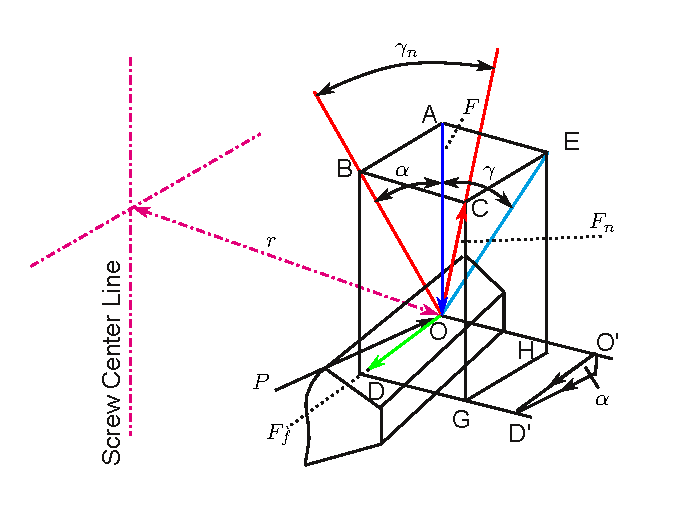
\includegraphics{Screw_sketch}
    \end{center}
    \caption{3D screw thread sketch.}
    \label{fig:screw_sketch_3D}
  \end{figure}

\end{enumerate}



\section{Shapes}
\label{sec:Shape}
The \hty{Shape} entities are objects that return a value depending on one
(or two, for 2D shapes) dimensionless abscissa, ranging $ \sqbr{-1,1} $.
At present, only 1D shapes are used, by aerodynamic elements.
A \hty{Shape} input format is:
%\begin{verbatim}
\begin{Verbatim}[commandchars=\\\{\}]
    \bnt{shape_1D} ::= \bnt{shape_type} ,
        \bnt{shape_arglist}
\end{Verbatim}
%\end{verbatim}
The shapes currently available are:
\begin{enumerate}
    \item \kw{const}
%\begin{verbatim}
\begin{Verbatim}[commandchars=\\\{\}]
    \bnt{shape_type} ::= \kw{const}

    \bnt{shape_arglist} ::= \bnt{const_value}
\end{Verbatim}
%\end{verbatim}
\begin{align}
	f = \nt{const\_value}
\end{align}

    \item \kw{piecewise const}
%\begin{verbatim}
\begin{Verbatim}[commandchars=\\\{\}]
    \bnt{shape_type} ::= \kw{piecewise const}

    \bnt{shape_arglist} ::=
        \bnt{number_of_points} , 
            \bnt{abscissa} , \bnt{value}
            [ , ... ]
\end{Verbatim}
%\end{verbatim}
\begin{subequations}
\begin{align}
	f(\xi) &= \nt{value}_1	&& \xi \le \nt{abscissa}_1
	\\
	f(\xi) &= \nt{value}_i	&& \nt{abscissa}_i \le \xi < \nt{abscissa}_{i+1}
	\\
	f(\xi) &= \nt{value}_N	&& \nt{abscissa}_N \le \xi
\end{align}
\end{subequations}

    \item \kw{linear}
%\begin{verbatim}
\begin{Verbatim}[commandchars=\\\{\}]
    \bnt{shape_type} ::= \kw{linear}

    \bnt{shape_arglist} ::=
        \bnt{value_at_-1} , 
        \bnt{value_at_1}
\end{Verbatim}
%\end{verbatim}
\begin{align}
	f(\xi) &= \frac{\nt{value\_at\_-1} + \nt{value\_at\_1}}{2}
		+ \frac{\nt{value\_at\_-1} - \nt{value\_at\_1}}{2} \xi
\end{align}

    \item \kw{piecewise linear}
%\begin{verbatim}
\begin{Verbatim}[commandchars=\\\{\}]
    \bnt{shape_type} ::= \kw{piecewise linear}

    \bnt{shape_arglist} ::=
        \bnt{number_of_points} , 
            \bnt{abscissa} , \bnt{value}
            [ , ... ]
\end{Verbatim}
%\end{verbatim}
\begin{subequations}
\begin{align}
	f(\xi) &= \nt{value}_1	&& \xi \le \nt{abscissa}_1
	\\
	f(\xi) &=
		\nt{value}_i \, \, \frac{\nt{abscissa}_{i+1} - \xi}{\nt{abscissa}_{i+1} - \nt{abscissa}_i}
	\nonumber \\
		&
		+ \nt{value}_{i+1} \, \frac{\xi - \nt{abscissa}_i}{\nt{abscissa}_{i+1} - \nt{abscissa}_i}
		&& \nt{abscissa}_i \le \xi < \nt{abscissa}_{i+1}
	\\
	f(\xi) &= \nt{value}_N	&& \nt{abscissa}_N \le \xi
\end{align}
\end{subequations}

    \item \kw{parabolic}
%\begin{verbatim}
\begin{Verbatim}[commandchars=\\\{\}]
    \bnt{shape_type} ::= \kw{parabolic}

    \bnt{shape_arglist} ::=
        \bnt{value_at_-1} , 
        \bnt{value_at_0} , 
        \bnt{value_at_1}
\end{Verbatim}
%\end{verbatim}
\begin{align}
	f(\xi) &= \nt{value\_at\_-1} \cdot \xi\plbr{\xi - 1}
		+ \nt{value\_at\_0} \cdot \plbr{1 - \xi^2}
		+ \nt{value\_at\_1} \cdot \xi\plbr{\xi + 1}
\end{align}

\end{enumerate}
This form of input has been chosen since, being the shapes mainly used to
interpolate values, it looks more ``natural'' to insert the mapping values
at characteristic points.
For \kw{piecewise linear} shapes, there must be 
\nt{number\_of\_points} pairs of absciss\ae\ and values; absciss\ae\
must be in the range $\sqbr{-1,1}$, in strict ascending order.


\section{Constitutive Laws}\label{sec:ConstitutiveLaw}
Implements the type \texttt{\ty{ConstitutiveLaw}\be{\bnt{Entity}, \bnt{DerivativeOfEntity}}}.
Every time a ``deformable'' entity requires a constitutive law, a template
constitutive law is read. This has been implemented by means of C++
templates in order to allow the definition of a general constitutive law
when possible.
The ``deformable'' elements at present are:
\begin{itemize}
\item \htmlref{\kw{rod}}{sec:EL:STRUCT:JOINT:ROD}
	and
	\htmlref{\kw{genel} \kw{spring}}{sec:EL:GENEL:SPRING}
	and related elements (1D);
\item \htmlref{\kw{deformable hinge}}{sec:EL:JOINT:DEFORMABLEHINGE}
	and \htmlref{\kw{deformable displacement joint}}{sec:EL:JOINT:DEFORMABLEDISP}
	elements (3D);
\item \htmlref{\kw{deformable joint}}{sec:EL:JOINT:DEFORMABLEJOINT}, \htmlref{\kw{beam}}{sec:EL:BEAM} and \htmlref{\kw{solid}}{sec:EL:SOLID}
        elements (6D).
\item \htmlref{\kw{solid}}{sec:EL:SOLID}
  elements for incompressible constitutive laws (7D).
\item \htmlref{\kw{solid}}{sec:EL:SOLID}
	elements for constitutive laws subject to finite strain (9D).
\end{itemize}

Constitutive laws are also used in non-structural components,
to allow some degree of generality in defining input/output relationships.
Some constitutive laws are meaningful only when related to some precise
dimensionality. 
In some special cases, general purpose (\htmlref{\kw{genel}}{sec:EL:GENEL})
elements use 1D constitutive laws to express an arbitrary dependence
of some value on a scalar state of the system.
Table~\ref{tab:CONST-LAW-DIM} shows the availability of each constitutive law.

The meaning of the input and output parameters of a constitutive law
is dictated by the entity that uses it.
In general, the user should refer to the element the constitutive law
is being instantiated for, in order to understand what the input
and the output parameters are supposed to be.

Usually, constitutive laws can be directly defined when required,
according to the definition of an element.
However, the special card described in Section~\ref{sec:CONSTITUTIVE-LAW}
allows to define constitutive laws stand-alone, and attach them
to the elements by means of the following mechanism:
%\begin{verbatim}
\begin{Verbatim}[commandchars=\\\{\}]
    \bnt{constitutive_law} ::=
        \{ \bnt{constitutive_law_definition} | \kw{reference} , \bnt{label} \}
\end{Verbatim}
%\end{verbatim}
where \nt{<constitutive\_law\_definition>} is described in the following,
while \nt{<label>} is the label of a previously defined constitutive law
of the appropriate dimensionality, as described
in Section~\ref{sec:CONSTITUTIVE-LAW}.



\begin{table}%[H]
    \newlength{\constlawwidth}
    \setlength{\constlawwidth}{70mm}
    \centering
    \caption{Constitutive laws dimensionality}\label{tab:CONST-LAW-DIM}
    \begin{tabular}{l|c|c|c|c|c} 
        \hline
        \multicolumn{1}{c}{\textbf{Constitutive law}} &
	\multicolumn{1}{c}{\textbf{1D}} &
	\multicolumn{1}{c}{\textbf{3D}} &
	\multicolumn{1}{c}{\textbf{6D}} &
        \multicolumn{1}{c}{\textbf{7D}} &
        \multicolumn{1}{c}{\textbf{9D}} \\
	\hline
	\kw{linear elastic}, \kw{linear elastic isotropic}			& $\surd$ & $\surd$ & $\surd$ &         & \\
	\kw{linear elastic generic}						& $\surd$ & $\surd$ & $\surd$ &         & \\
	\kw{linear elastic generic axial torsion coupling}			&         &         & $\surd$ &         & \\
	\kw{cubic elastic generic}						& $\surd$ & $\surd$ &         &         & \\
	\kw{inverse square elastic}						& $\surd$ &         &         &         & \\
	\kw{log elastic}							& $\surd$ &         &         &         & \\
	\kw{linear elastic bistop}						& $\surd$ & $\surd$ & $\surd$ &         & \\
	\kw{double linear elastic}						& $\surd$ & $\surd$ &         &         & \\
	\kw{isotropic hardening elastic}					& $\surd$ & $\surd$ & $\surd$ &         & \\
	\kw{scalar function elastic}, \kw{scalar function elastic isotropic}	& $\surd$ & $\surd$ & $\surd$ &         & \\
	\kw{scalar function elastic orthotropic}				& $\surd$ & $\surd$ & $\surd$ &         & \\
	\kw{linear viscous}, \kw{linear viscous isotropic}			& $\surd$ & $\surd$ & $\surd$ &         & \\
	\kw{linear viscous generic}						& $\surd$ & $\surd$ & $\surd$ &         & \\
	\kw{linear viscoelastic}, \kw{linear viscoelastic isotropic}		& $\surd$ & $\surd$ & $\surd$ &         & \\
	\kw{linear viscoelastic generic}					& $\surd$ & $\surd$ & $\surd$ &         & \\
	\kw{linear time variant viscoelastic generic}				& $\surd$ & $\surd$ & $\surd$ &         & \\
	\kw{linear viscoelastic generic axial torsion coupling}			&         &         & $\surd$ &         & \\
	\kw{cubic viscoelastic generic}						& $\surd$ & $\surd$ &         &         & \\
	\kw{double linear viscoelastic}						& $\surd$ & $\surd$ &         &         & \\
	\kw{turbulent viscoelastic}						& $\surd$ &         &         &         & \\
	\kw{linear viscoelastic bistop}						& $\surd$ & $\surd$ & $\surd$ &         & \\
	\kw{shock absorber}							& $\surd$ &         &         &         & \\
	\kw{symbolic elastic}							& $\surd$ & $\surd$ & $\surd$ &         & \\
	\kw{symbolic viscous}							& $\surd$ & $\surd$ & $\surd$ &         & \\
	\kw{symbolic viscoelastic}						& $\surd$ & $\surd$ & $\surd$ &         & \\
	\kw{ann elastic}							& $\surd$ & $\surd$ & $\surd$ &         & \\
	\kw{ann viscoelastic}							& $\surd$ & $\surd$ & $\surd$ &         & \\
	\kw{nlsf elastic}							& $\surd$ & $\surd$ & $\surd$ &         & \\
	\kw{nlsf viscous}							& $\surd$ & $\surd$ & $\surd$ &         & \\
	\kw{nlsf viscoelastic}							& $\surd$ & $\surd$ & $\surd$ &         & \\
	\kw{nlp elastic}							& $\surd$ & $\surd$ & $\surd$ &         & \\
	\kw{nlp viscous}							& $\surd$ & $\surd$ & $\surd$ &         & \\
	\kw{nlp viscoelastic}							& $\surd$ & $\surd$ & $\surd$ &         & \\
        \kw{hookean linear elastic isotropic}                                   &         &         & $\surd$ & $\surd$ & \\
        \kw{hookean linear viscoelastic isotropic}                              &         &         & $\surd$ &         & \\        
        \kw{neo hookean elastic}                                                &         &         & $\surd$ &         & \\
        \kw{neo hookean viscoelastic}                                           &         &         & $\surd$ &         & \\
        \kw{mooney rivlin elastic}                                              &         &         & $\surd$ & $\surd$ & $\surd$ \\
        \kw{bilinear isotropic hardening}                                       &         &         & $\surd$ & $\surd$ & \\
        \kw{linear viscoelastic maxwell 1}                                      &         & $\surd$ & $\surd$ &         & \\
        \kw{linear viscoelastic maxwell n}                                      &         & $\surd$ & $\surd$ &         & \\
        \kw{mfront small strain}                                                &         &         & $\surd$ &         & \\
        \kw{mfront finite strain}                                               &         &         &         &         & $\surd$ \\
        \hline
	\multicolumn{6}{c}{} \\
	\hline
        \multicolumn{1}{c}{\textbf{Constitutive law wrapper}} &
	\multicolumn{1}{c}{\textbf{1D}} &
	\multicolumn{1}{c}{\textbf{3D}} &
	\multicolumn{1}{c}{\textbf{6D}} &
        \multicolumn{1}{c}{\textbf{7D}} &
        \multicolumn{1}{c}{\textbf{9D}} \\
	\hline
	\kw{array} (wrapper)							& $\surd$ & $\surd$ & $\surd$ &         \\
	\kw{axial} (wrapper)							&         & $\surd$ &         &         \\
	\kw{bistop} (wrapper)							& $\surd$ & $\surd$ & $\surd$ &         \\
	\kw{drive caller} (wrapper)						& $\surd$ & $\surd$ & $\surd$ &         \\
	\kw{invariant angular} (wrapper)					&         & $\surd$ &         &         \\
        \hline
    \end{tabular}
\end{table}

The constitutive laws are entered as follows:
%\begin{verbatim}
\begin{Verbatim}[commandchars=\\\{\}]
    \bnt{constitutive_law_definition} ::= \bnt{specific_const_law}
        [ , \kw{prestress} , (\ty{Entity}) \bnt{prestress} ]
        [ , \kw{prestrain} , (\htybent{TplDriveCaller}{Entity}) \bnt{prestrain} ]

    \bnt{specific_const_law} ::= \bnt{const_law_name} ,
        \bnt{const_law_data}
\end{Verbatim}
%\end{verbatim}
where \nt{const\_law\_name} is the name of the constitutive law and
\nt{const\_law\_data} depends on the specific constitutive law. 
The latter fields, whose type depends on the dimensionality of the
constitutive law, are optional, under the assumption that the
constitutive law is the last portion of a card, or that any ambiguity 
can be avoided.
The data specific to the currently available constitutive laws must be
entered as follows:


\subsection{Linear elastic, linear elastic isotropic}
%\begin{verbatim}
\begin{Verbatim}[commandchars=\\\{\}]
    \bnt{specific_const_law} ::= \kw{linear elastic} [ \kw{isotropic} ] , 
        (\ty{real}) \bnt{stiffness}
\end{Verbatim}
%\end{verbatim}
the isotropic stiffness coefficient; the word \kw{isotropic}
can be omitted, essentially because it has no meaning
for scalar constitutive laws.

\paragraph{Example.} \
\begin{verbatim}
    constitutive law: 1, name, "scalar isotropic law",
        1, linear elastic, 1.e9;
    constitutive law: 2, name, "3D isotropic law",
        3, linear elastic isotropic, 1.e9;
    constitutive law: 3, name, "6D isotropic law",
        6, linear elastic isotropic, 1.e9;
\end{verbatim}
  
  
\subsection{Linear elastic generic}
%\begin{verbatim}
\begin{Verbatim}[commandchars=\\\{\}]
    \bnt{specific_const_law} ::= \kw{linear elastic generic} ,
        (\ty{DerivativeOfEntity}) \bnt{stiffness}
\end{Verbatim}
%\end{verbatim}
the stiffness matrix. In case of 1D, the type is scalar, 
and there is no distinction between \kw{generic} and \kw{isotropic}, 
while, in case of $N \times 1$ vectors, the type is the corresponding 
$N \times N$ matrix.

\paragraph{Example.} \
\begin{verbatim}
    constitutive law: 1, name, "scalar isotropic law",
        1, linear elastic generic, 1.e9;
    constitutive law: 2, name, "3D isotropic law",
        3, linear elastic generic,
            sym, 1.e9,  0.,    0.,
                        1.e6, -1.e5,
                               1.e6;
    constitutive law: 3, name, "6D isotropic law",
        6, linear elastic generic,
            diag, 1.e9, 1.e9, 1.e9, 1.e6, 1.e6, 1.e6;
\end{verbatim}
  

\subsection{Linear elastic generic axial torsion coupling}
\label{sec:ConstitutiveLaw:LINEAR-ELASTIC-GENERIC-AXIAL-TORSION-COUPLING}
%\begin{verbatim}
\begin{Verbatim}[commandchars=\\\{\}]
    \bnt{specific_const_law} ::= 
        \kw{linear elastic generic axial torsion coupling} ,
            (\ty{DerivativeOfEntity}) \bnt{stiffness} ,
            (\ty{real}) \bnt{coupling_coefficient}
\end{Verbatim}
%\end{verbatim}
this is defined only for $6 \times 1$ vectors, where the torsion stiffness,
coefficient $ a_{44} $ in the stiffness matrix, depends linearly on 
the axial strain, $ \varepsilon_1 $, by means of 
\nt{coupling\_coefficient}, i.e.\ the run-time torsion stiffness is 
\begin{align}
	a_{44}
	&=
	GJ + \nt{coupling\_coefficient} \cdot \varepsilon_1 .
\end{align}
This \nt{<coupling\_coefficient>}, in the classical nonlinear beam theory,
is estimated according to some geometric property \cite{HOUBOLT-BROOKS-1957};
a general approach to the computation of prestressed beam properties
is presented in \cite{BORRI-MERLINI}, which is implemented in some versions
of the ANBA software.

\subsection{Cubic elastic generic}
%\begin{verbatim}
\begin{Verbatim}[commandchars=\\\{\}]
    \bnt{specific_const_law} ::= 
        \kw{cubic elastic generic}
            (\ty{Entity}) \bnt{stiffness_1} ,
            (\ty{Entity}) \bnt{stiffness_2} ,
            (\ty{Entity}) \bnt{stiffness_3}
\end{Verbatim}
%\end{verbatim}
this is defined only for scalar and $3 \times 1$ vectors; the constitutive
law is written according to the formula
\begin{align}
	f
	&=
	\nt{stiffness\_1} \cdot \varepsilon
	+ \nt{stiffness\_2} \cdot \shbr{\varepsilon}\varepsilon
	+ \nt{stiffness\_3} \cdot \varepsilon^3
\end{align}
%and it is mainly intended for use with human body models 
%where the stiffness of the joints is typically given in this form.
%
%\textbf{FIXME: check!}

\subsection{Inverse square elastic}
%\begin{verbatim}
\begin{Verbatim}[commandchars=\\\{\}]
    \bnt{specific_const_law} ::= \kw{inverse square elastic} ,
        (\ty{real}) \bnt{stiffness} , (\ty{real}) \bnt{ref_length}
\end{Verbatim}
%\end{verbatim}
this is defined only for scalars. The force is defined as:
\begin{align}
    f &= \frac{\nt{stiffness}}{\plbr{\nt{ref\_lenght} \cdot \plbr{1 + \varepsilon}}^2}
\end{align}
  
\subsection{Log elastic}
%\begin{verbatim}
\begin{Verbatim}[commandchars=\\\{\}]
    \bnt{specific_const_law} ::= \kw{log elastic} ,
        (\ty{DerivativeOfEntity}) \bnt{stiffness}
\end{Verbatim}
%\end{verbatim}
this is defined only for scalars. The force is defined as:
\begin{align}
    f &= \nt{stiffness} \cdot \llk{log}\plbr{1 + \varepsilon}
\end{align}
  
\subsection{Linear elastic bistop}
%\begin{verbatim}
\begin{Verbatim}[commandchars=\\\{\}]
    \bnt{specific_const_law} ::= \kw{linear elastic bistop} ,
        (\ty{DerivativeOfEntity}) \bnt{stiffness} ,
        [ \kw{initial status} , \{ \kw{inactive} | \kw{active} | (\ty{bool}) \bnt{status} \} , ]
        (\hty{DriveCaller}) \bnt{activating_condition} ,
        (\hty{DriveCaller}) \bnt{deactivating_condition}
\end{Verbatim}
%\end{verbatim}
  
\subsection{Double linear elastic}
%\begin{verbatim}
\begin{Verbatim}[commandchars=\\\{\}]
    \bnt{specific_const_law} ::= \kw{double linear elastic} ,
        (\ty{real}) \bnt{stiffness_1} ,
        (\ty{real}) \bnt{upper_strain} ,
        (\ty{real}) \bnt{lower_strain} ,
        (\ty{real}) \bnt{stiffness_2}
        [, \kw{third stiffness} \bnt{stiffness_3}]
\end{Verbatim}
%\end{verbatim}
this is defined for scalar and $3 \times 1$ vectors. In the scalar case the
meaning of the entries is straightforward,
while in case of $3 \times 1$ vectors the constitutive law is isotropic
but in the local direction 3, where, in case of strain
out of the upper or lower bound, the \nt{stiffness\_2} is used.
If \kw{third stiffness} is given, its value is used in the strain region 
below $\nt{lower\_strain}$.
\subsection{Isotropic hardening elastic}
%\begin{verbatim}
\begin{Verbatim}[commandchars=\\\{\}]
    \bnt{specific_const_law} ::= \kw{isotropic hardening elastic} ,
        (\ty{real}) \bnt{stiffness} ,
        (\ty{real}) \bnt{reference_strain}
        [ , \kw{linear stiffness} , \bnt{linear_stiffness} ]
\end{Verbatim}
%\end{verbatim}
this constitutive law is defined as follows:
\begin{displaymath}
    f \ = \ \nt{stiffness} \ \frac{
        \beta + \alpha\shbr{\T{\varepsilon}}^2
    }{
        1 + \alpha\shbr{\T{\varepsilon}}^2
    }\varepsilon
\end{displaymath}
where $\alpha=3/\shbr{\nt{reference\_strain}}^2$,
and $\beta=\nt{linear\_stiffness}/\nt{stiffness}$.
The resulting constitutive law, in the scalar case,
is somewhat soft/hard when $\beta$ is lower/greater than 1
and $\shbr{\varepsilon}$ is smaller than \nt{reference\_strain},
approaching \nt{linear\_stiffness} when $\varepsilon\rightarrow{0}$,
while it grows to quasi-linear for larger $\shbr{\varepsilon}$, 
with slope $\nt{stiffness}$.

\subsection{Scalar function elastic, scalar function elastic isotropic}
This constitutive law is based on a 
\hty{ScalarFunction}
to represent an analytical force-displacement curve 
of a single variable that is automatically differentiated 
to compute the slope of the curve, namely the local stiffness.
%\begin{verbatim}
\begin{Verbatim}[commandchars=\\\{\}]
    \bnt{specific_const_law} ::= \kw{scalar function elastic} [ \kw{isotropic} ] ,
        (\htmlref{\ty{DifferentiableScalarFunction}}{sec:ScalarFunction}) \bnt{function}
\end{Verbatim}
%\end{verbatim}
this constitutive law is defined as follows:
\begin{displaymath}
	f_i = \nt{function}\plbr{\T{\varepsilon}_i}
\end{displaymath}
the force is computed for each direction as a function of the respective
strain component using the same function.
When used for 1D elements, the word \kw{isotropic} can be omitted.

\bigskip
\noindent
\emph{Note: the \kw{Scalar function elastic} and the \kw{scalar function elastic isotropic} constitutive laws do not support \kw{prestress} nor \kw{prestrain}}.

\subsection{Scalar function elastic orthotropic}
%\begin{verbatim}
\begin{Verbatim}[commandchars=\\\{\}]
    \bnt{specific_const_law} ::= \kw{scalar function elastic} [ \kw{orthotropic} ] ,
        \{ (\htmlref{\ty{DifferentiableScalarFunction}}{sec:ScalarFunction}) \bnt{function} | \kw{null} \}
        [ , ... ]
\end{Verbatim}
%\end{verbatim}
this constitutive law is defined as follows:
\begin{displaymath}
	f_i = \nt{function}_i \plbr{\T{\varepsilon}_i}
\end{displaymath}
the force is computed for each direction as a function of the respective
strain component using a specific function for each component.
If no force ought to be used for a direction, for example because 
that direction is constrained by a kinematic joint, the keyword \kw{null}
can be used to indicate that no function is expected for that component.
When used for 1D elements, the word \kw{orthotropic} can be omitted;
note that in this case a \kw{scalar function elastic isotropic}
constitutive law is actually instantiated.

\paragraph{Example.} \
\begin{verbatim}
    scalar function: "myfunc", multilinear,
        -1., -100.,
        -.5, -70.,
        0., 0.,
        .5, 70.,
        1., 100.;
    constitutive law: 1000, 3,
        scalar function elastic orthotropic,
            null,
            null,
            "myfunc";
\end{verbatim}
indicates that the constitutive law is only defined in direction 3 
as a multilinear function.

\bigskip
\noindent
\emph{Note: the \kw{Scalar function elastic orthotropic} constitutive law does not support \kw{prestress} nor \kw{prestrain}}.

\subsection{Linear viscous, linear viscous isotropic}
%\begin{verbatim}
\begin{Verbatim}[commandchars=\\\{\}]
    \bnt{specific_const_law} ::= \kw{linear viscous} [ \kw{isotropic} ] , 
        (\ty{real}) \bnt{viscosity}
\end{Verbatim}
%\end{verbatim}
the linear viscous coefficient. \\
{\em 
    Note: this constitutive law does not require any prestrain template
    drive caller.
}
  
\subsection{Linear viscous generic}
%\begin{verbatim}
\begin{Verbatim}[commandchars=\\\{\}]
    \bnt{specific_const_law} ::= \kw{linear viscous generic} , 
        (\ty{DerivativeOfEntity}) \bnt{viscosity}
\end{Verbatim}
%\end{verbatim}
the linear viscous $N \times N $ matrix. \\
{\em 
    Note: this constitutive law does not require any prestrain template
    drive caller.
}
  
\subsection{Linear viscoelastic, linear viscoelastic isotropic}
%\begin{verbatim}
\begin{Verbatim}[commandchars=\\\{\}]
    \bnt{specific_const_law} ::= \kw{linear viscoelastic} [ \kw{isotropic} ] ,
        (\ty{real}) \bnt{stiffness} ,
        \{ (\ty{real}) \bnt{viscosity}
            | \kw{proportional} , (\ty{real}) \bnt{factor} \}
\end{Verbatim}
%\end{verbatim}
the isotropic stiffness and viscosity coefficients.
If \kw{proportional} is given, then
$\nt{viscosity} = \nt{factor} \cdot \nt{stiffness}$.
  
\subsection{Linear viscoelastic generic}
%\begin{verbatim}
\begin{Verbatim}[commandchars=\\\{\}]
    \bnt{specific_const_law} ::= \kw{linear viscoelastic generic} ,  
        (\ty{DerivativeOfEntity}) \nt{stiffness} ,
        \{ (\ty{DerivativeOfEntity}) \bnt{viscosity} 
            | \kw{proportional} , (\ty{real}) \bnt{factor} \}
\end{Verbatim}
%\end{verbatim}
the linear stiffness and viscosity $N \times N$ matrices.
If \kw{proportional} is given, then
$\nt{viscosity} = \nt{factor} \cdot \nt{stiffness}$.
  
\subsection{Linear time variant viscoelastic generic}
%\begin{verbatim}
\begin{Verbatim}[commandchars=\\\{\}]
    \bnt{specific_const_law} ::= \kw{linear time variant viscoelastic generic} ,
        (\ty{DerivativeOfEntity}) \bnt{stiffness} ,
        (\hty{DriveCaller}) \bnt{stiffness_scale} ,
        \{ (\ty{DerivativeOfEntity}) \bnt{viscosity}
            | \kw{proportional} , (\ty{real}) \bnt{factor} \} ,
        \{ \kw{same} | (\hty{DriveCaller}) \bnt{viscosity_scale} \}
\end{Verbatim}
%\end{verbatim}
the linear stiffness and viscosity matrices are multiplied
by the respective scale factors,
\begin{align}
	\T{f} &= \nt{stiffness} \cdot \nt{stiffness\_scale} \cdot \T{\varepsilon}
		+ \nt{viscosity} \cdot \nt{viscosity\_scale} \cdot \dot{\T{\varepsilon}}
	.
\end{align}
If \kw{proportional} is given, then
$\nt{viscosity} = \nt{factor} \cdot \nt{stiffness}$.
The keyword \kw{same} uses for the drive caller \nt{viscosity\_scale} the same drive caller \nt{stiffness\_scale} defined for the elastic portion of the constitutive law.

\paragraph{Example.}
\begin{verbatim}
    linear time variant viscoelastic,
        1000., cosine, 2., pi/.2, .1/2, half, 1.,
        100., cosine, 2., pi/.2, 1/2, half, 1.
\end{verbatim}
At 2s, the stiffness grows of 10\% from the nominal value in .2s,
while the damping doubles.
See Section~\ref{sec:DriveCaller} for details on the syntax
of \hty{DriveCaller} entities.

Beware that arbitrarily changing the stiffness
and the damping of an elastic component during the execution
of the simulation may have no physical meaning.
The intended use of this feature is for tailoring the analysis;
for example, a higher damping level may be desirable to smooth out
a non-physical transient, and later return to the appropriate damping value.
  
\subsection{Linear viscoelastic generic axial torsion coupling}
%\begin{verbatim}
\begin{Verbatim}[commandchars=\\\{\}]
    \bnt{specific_const_law} ::= 
        \kw{linear viscoelastic generic axial torsion coupling} ,
            (\ty{DerivativeOfEntity}) \bnt{stiffness} ,
            \{ (\ty{DerivativeOfEntity}) \bnt{viscosity} 
                | \kw{proportional} , (\ty{real}) \bnt{factor} \}
            (\ty{real}) \bnt{coupling_coefficient}
\end{Verbatim}
%\end{verbatim}
this is defined only for $6 \times 1$ vectors; it is the viscoelastic 
extension of the 
\hyperref{\kw{linear elastic generic axial torsion coupling} constitutive law}{\kw{linear elastic generic axial torsion coupling} constitutive law (see Section~}{)}{sec:ConstitutiveLaw:LINEAR-ELASTIC-GENERIC-AXIAL-TORSION-COUPLING}.


\subsection{Cubic viscoelastic generic}
%\begin{verbatim}
\begin{Verbatim}[commandchars=\\\{\}]
    \bnt{specific_const_law} ::= 
        \kw{cubic elastic generic}
            (\ty{Entity}) \bnt{stiffness_1} ,
            (\ty{Entity}) \bnt{stiffness_2} ,
            (\ty{Entity}) \bnt{stiffness_3} ,
            (\ty{DerivativeOfEntity}) \bnt{viscosity}
\end{Verbatim}
%\end{verbatim}
this is defined only for scalar and $3 \times 1$ vectors; the constitutive
law is written according to the formula
\begin{displaymath}
	f = \nt{stiffness\_1} \cdot \varepsilon
	+ \nt{stiffness\_2} \cdot \shbr{\varepsilon}\varepsilon
	+ \nt{stiffness\_3} \cdot \varepsilon^3
	+ \nt{viscosity} \cdot \dot{\varepsilon}
\end{displaymath}
and it is mainly intended for use with human body models 
where the stiffness of the joints is typically given in this form.

\subsection{Double linear viscoelastic}
%\begin{verbatim}
\begin{Verbatim}[commandchars=\\\{\}]
    \bnt{specific_const_law} ::= \kw{double linear viscoelastic} ,
        (\ty{real}) \bnt{stiffness_1} ,
        (\ty{real}) \bnt{upper_strain} ,
        (\ty{real}) \bnt{lower_strain} ,
        (\ty{real}) \bnt{stiffness_2} ,
        (\ty{real}) \bnt{viscosity}
        [ , \kw{second damping} , (\ty{real}) \bnt{viscosity_2} ]
\end{Verbatim}
%\end{verbatim}
this is analogous to the \kw{double linear elastic} constitutive law,
except for the isotropic viscosity term.
The second viscosity value is used when the strain is outside the
$\nt{lower\_strain} - \nt{upper\_strain}$ range.

When this constitutive law is used with $3 \times 1$ vectors, 
the double linear elastic and viscous term only applies to component 3.
  
\subsection{Turbulent viscoelastic}
%\begin{verbatim}
\begin{Verbatim}[commandchars=\\\{\}]
    \bnt{specific_const_law} ::= \kw{turbulent viscoelastic} ,
        (\ty{real}) \bnt{stiffness} ,
        (\ty{real}) \bnt{parabolic_viscosity}
        [ , (\ty{real}) \bnt{threshold}
            [ , (\ty{real}) \bnt{linear_viscosity} ] ]
\end{Verbatim}
%\end{verbatim}
the constitutive law has the form:
\begin{displaymath}
    \T{f} \ = \ \nt{stiffness} \ \T{\varepsilon} + k \ \dot{\T{\varepsilon}}
\end{displaymath}
where:
\begin{displaymath}
    k = \lcubr{\matr{lcr}{
        \nt{linear\_viscosity} & & 
            \shbr{\dot{\T{\varepsilon}}} \leq \nt{threshold} \\
        \nt{parabolic\_viscosity} & &
            \shbr{\T{\dot{\varepsilon}}} > \nt{threshold}
    }}
\end{displaymath}
if \nt{threshold} is null, or not defined, the constitutive law is always
parabolic. If the \nt{linear\_viscosity} is not defined, it is
computed based on \nt{parabolic\_viscosity} and on 
\nt{threshold} to give a continuous force curve (with discontinuous slope).
Otherwise, it can be set by the user to give a discontinuous force curve,
as observed in some fluids at intermediate Reynolds number.

\subsection{Linear viscoelastic bistop}
%\begin{verbatim}
\begin{Verbatim}[commandchars=\\\{\}]
    \bnt{specific_const_law} ::= \kw{linear viscoelastic bistop} ,
        (\ty{DerivativeOfEntity}) \bnt{stiffness} ,
        (\ty{DerivativeOfEntity}) \bnt{viscosity} ,
        [ \kw{initial status} , \{ \kw{inactive} | \kw{active} | (\ty{bool}) \bnt{status} \} , ]
        (\hty{DriveCaller}) \bnt{activating_condition} ,
        (\hty{DriveCaller}) \bnt{deactivating_condition}
\end{Verbatim}
%\end{verbatim}
  
\subsection{GRAALL damper}
This very experimental constitutive law, based on a nonlinear model
for a hydraulic damper to be used in landing gear modeling,
has been moved to \texttt{module-damper-graall}.

\subsection{shock absorber}\label{sec:CL:SHOCK-ABSORBER}
This constitutive law implements a landing gear hydraulic shock absorber:
%\begin{verbatim}
\begin{Verbatim}[commandchars=\\\{\}]
    \bnt{specific_const_law} ::= \kw{shock absorber} ,
        [ \kw{prestrain} , \bnt{value} , ]
        \bnt{reference_pressure} ,
        \bnt{reference_area_for_force_computation} ,
        \bnt{interaction_coefficient} ,
        \bnt{polytropic_exponent} ,
        [ \kw{epsilon max} , \bnt{upper_strain_bound} , ]
        [ \kw{epsilon min} , \bnt{lower_strain_bound} , ]
        [ \kw{penalty} , \bnt{penalty_factor_for_strain} , 
            \bnt{penalty_factor_for_strain_rate} , ]
        [ \kw{metering} , (\ty{DriveCaller})\bnt{metering_area} ,
            [ \kw{negative} , (\ty{DriveCaller})\bnt{metering_area_for_negative_strain_rate} , ]
        [ \kw{orifice} , (\ty{DriveCaller})\bnt{orifice_area} , ]
        \bnt{fluid_area} ,
        \bnt{fluid_density} ,
        \bnt{drag_coefficient_/_reference_length} # scales strain rate to velocity
        [ , \kw{friction} , \bnt{reference_epsilon_prime} ,
             \bnt{friction_amplitude_coefficient} ]
\end{Verbatim}
%\end{verbatim}
where
\begin{itemize}
\item the \nt{interaction\_coefficient} is represented by
\begin{displaymath}
	\nt{kinematic scale} \cdot \frac{L A}{V_0}
\end{displaymath}
where \nt{kinematic scale} is the ratio between the stroke
of the shock absorber and that of the gas;
\item \nt{upper\_strain\_bound} is the upper strain bound; it must be
at least larger than the prestrain, and defaults to 0,
i.e.\ the shock absorber, at rest, is assumed to be fully
extended;
\item \nt{lower\_strain\_bound} is the lower strain bound; it must be
at least smaller than the prestrain, and defaults to -0.5, 
i.e.\ the shock absorber is assumed to allow a contraction
equal to half its full length;
\item the \nt{penalty\_factor\_for\_strain} defaults to 1e+9;
it is active only when strain bounds are violated;
\item the \nt{penalty\_factor\_for\_strain\_rate} defaults to 0;
it is active only when strain bounds are violated;
\item the \nt{metering\_area} is given by a \hty{DriveCaller} 
and is strain dependent; if the keyword \kw{negative} is used, 
then the \nt{metering\_area\_for\_negative\_strain\_rate} is used
when the strain rate is negative, i.e.\ the shock absorber
is being compressed, while \nt{metering\_area} is used only
when the shock absorber is extending;
\item the \kw{orifice} drive determines the area of an
additional orifice, which essentially depends on the sign
of the strain rate; it is used to implement relief valves;
\item ...
\end{itemize}
This constitutive law contributes to the output of the element
it is associated with.
The name associated with each output contribution can be used to reference
the corresponding value as element private data.
The contributions are
\begin{enumerate}
\item \kw{"p"} gas pressure;
\item \kw{"A"} metering area;
\item \kw{"Fe"} elastic force;
\item \kw{"Fv"} viscous force.
\end{enumerate}

\subsection{symbolic elastic}\label{sec:CL:SYMBOLIC-ELASTIC}
The implementation  of the family of \kw{symbolic} constitutive laws
is based on GiNaC 
(\htmladdnormallink{\kw{http://www.ginac.de/}}{http://www.ginac.de/}),
a free software package for symbolic algebra manipulation.
It is essentially used to automatically differentiate
the user-supplied expression that describes the relationship
between the output and the input.

The syntax is
%\begin{verbatim}
\begin{Verbatim}[commandchars=\\\{\}]
    \bnt{specific_const_law} ::= \kw{symbolic elastic} ,
        \kw{epsilon} , " \bnt{epsilon} " [ , ... ] ,
        \kw{expression} , " \bnt{expression} " [ , ... ]
\end{Verbatim}
%\end{verbatim}
where \nt{epsilon} is the symbol describing the input
parameter as it will be used in \nt{expression}.

For constitutive laws with more than one dimension,
a string for each \nt{epsilon} and one for each \nt{expression}
are expected.  For example:
\begin{verbatim}
    # 1D symbolic constitutive law
    constitutive law: 1001, 1, symbolic elastic,
        epsilon, "eps",
        expression, "1000.*eps + 5.*eps^3";
    # 3D symbolic constitutive law
    constitutive law: 1003, 3, symbolic elastic,
        epsilon, "eps1", "eps2", "eps3",
        expression,
            "1000.*eps1 + 5.*eps1^3 - 10.*eps2*eps3",
            "1000.*eps2 + 5.*eps2^3 - 10.*eps3*eps1",
            "1000.*eps3 + 5.*eps3^3 - 10.*eps1*eps2";
\end{verbatim}

\emph{Note: right now, the symbols defined within the mathematical parser
are not available within symbolic constitutive laws.}

\subsection{symbolic viscous}\label{sec:CL:SYMBOLIC-VISCOUS}
The syntax is
%\begin{verbatim}
\begin{Verbatim}[commandchars=\\\{\}]
    \bnt{specific_const_law} ::= \kw{symbolic viscous} ,
        \kw{epsilon prime} , " \bnt{epsilon_prime} " [ , ... ] ,
        \kw{expression} , " \bnt{expression} " [ , ... ]
\end{Verbatim}
%\end{verbatim}
where \nt{epsilon\_prime} is the symbol describing the derivative
of the input parameter as it will be used in \nt{expression}.

For constitutive laws with more than one dimension,
a string for each \nt{epsilon\_prime} and one for each \nt{expression}
are expected.

\subsection{symbolic viscoelastic}\label{sec:CL:SYMBOLIC-VISCOELASTIC}
The syntax is
%\begin{verbatim}
\begin{Verbatim}[commandchars=\\\{\}]
    \bnt{specific_const_law} ::= \kw{symbolic viscoelastic} ,
        \kw{epsilon} , " \bnt{epsilon} " [ ,  ... ] ,
        \kw{epsilon prime} , " \bnt{epsilon_prime} " [ , ... ] ,
        \kw{expression} , " \bnt{expression} " [ , ... ]
\end{Verbatim}
%\end{verbatim}
where \nt{epsilon} and \nt{epsilon\_prime} are the symbols describing 
the input parameter and its derivative as they will be used
in \nt{expression}.

For constitutive laws with more than one dimension,
a string for each \nt{epsilon}, one for each \nt{epsilon\_prime},
and one for each \nt{expression} are expected.

\subsection{ann elastic}\label{sec:CL:ANN-ELASTIC}
The implementation  of the family of \kw{ann} constitutive laws
is based on an Artificial Neural Network library that is embedded in MBDyn.

The syntax is
%\begin{verbatim}
\begin{Verbatim}[commandchars=\\\{\}]
    \bnt{specific_const_law} ::= \kw{ann elastic} ,
        " \bnt{file_name} "
\end{Verbatim}
%\end{verbatim}
where the file \nt{file\_name} contains the parameters of the network.
What is mainly significant to users is the need to scale inputs and outputs
to match the amplitudes and possibly the offsets used in the training.
For this purpose, the last two rows of the input files contain coefficients
\begin{verbatim}
    b1 b0
    a1 a0
\end{verbatim}
which are used to scale the input $u$ and the output $y$ according
to the transformation
\begin{align}
	\overline{u} &= b_1 u + b_0 \\
	\overline{y} &= a_1 y + a_0
\end{align}
so that the actual output is
\begin{equation}
	y = \frac{f\plbr{b_1 u + b_0} - a_0}{a_1}
\end{equation}

\subsection{ann viscoelastic}\label{sec:CL:ANN-VISCOELASTIC}
The syntax is
%\begin{verbatim}
\begin{Verbatim}[commandchars=\\\{\}]
    \bnt{specific_const_law} ::= \kw{ann viscoelastic} ,
        " \bnt{file_name} "
\end{Verbatim}
%\end{verbatim}
where the file \nt{file\_name} contains the parameters of the network.

\subsection{nlsf viscoelastic}
\emph{This constitutive law was sponsored
by \htmladdnormallink{Hutchinson}{http://www.hutchinson.fr} CdR.}
\bigskip

For an $n$-dimensional constitutive law, it implements the formula
\begin{equation}
        f_i
        = \sum_{j=1,n} k'_{0ij} \varepsilon_j
        + f'_i\plbr{\varepsilon_i}
        + \sum_{j=1,n} k''_{0ij} \dot{\varepsilon}_j
        + f''_i\plbr{\dot{\varepsilon_i}}
        \label{eq:nlsf-cl}
\end{equation}
where $f'_i$ and $f''_i$ are arbitrary instances
of the \htmlref{\kw{scalar functions}}{sec:ScalarFunction} primitive,
which includes piecewise linear and spline regularization
of given data, while $k'_{0ij}$ and $k''_{0ij}$ are the constant
coefficients of a linear viscoelastic model, that account
for the cross-couplings between the stresses 
and the strains and strain rates.

Elastic and viscous variants are defined.
They differ from the viscoelastic one by only allowing
the specific fraction of the input data.

\paragraph{Syntax.}
\label{sec:CL:nlsf-syntax}
The syntax is
%\begin{verbatim}
\begin{Verbatim}[commandchars=\\\{\}]
    \bnt{specific_const_law} ::= \kw{nlsf viscoelastic} ,
        (\ty{DerivativeOfEntity}) \bnt{kappa_0'} ,
        \{ \kw{null} | (\hty{ScalarFunction}) \bnt{diag_force'} \}
        [ , ... ] ,
        \{ (\ty{DerivativeOfEntity}) \bnt{kappa_0''} | \kw{proportional} , \bnt{coef} \} ,
        \{ \kw{null} | (\hty{ScalarFunction}) \bnt{diag_force''} \}
        [ , ... ]

    \bnt{specific_const_law} ::= \kw{nlsf elastic} ,
        (\ty{DerivativeOfEntity}) \bnt{kappa_0'} ,
        \{ \kw{null} | (\hty{ScalarFunction}) \bnt{diag_force'} \}
        [ , ... ]

    \bnt{specific_const_law} ::= \kw{nlsf viscous} ,
        (\ty{DerivativeOfEntity}) \bnt{kappa_0''} ,
        \{ \kw{null} | (\hty{ScalarFunction}) \bnt{diag_force''} \}
        [ , ... ]
\end{Verbatim}
%\end{verbatim}
The terms \nt{kappa\_0'} and \nt{kappa\_0'{'}} are indicated as
\ty{DerivativeOfEntity} because in the generic case they are the result
of a differential operator that computes the derivative of the force vector
as function of the strain or strain rate vectors.
So, for a 3D constitutive law, the force, the strain and the strain rate
are $3\times 1$ vectors, while \nt{kappa\_0'} and \nt{kappa\_0'{'}}
are $3\times 3$ matrices.
Matrix input, in MBDyn, requires to write the whole set of coefficients,
row-wise; however, it can be described in many synthetic manners if
matrices have some special properties, as typical linear constitutive laws do.

For example, symmetric, diagonal and empty matrices have specific
short forms; in the $3\times 3$ case they are
\begin{verbatim}
        # generic 3x3 matrix:
        10., -2., -2.,
        -2., 20., -8.,
        -2., -8., 20.

        # symmetric 3x3 matrix (same as above matrix):
        sym,
        10., -2., -2.,
             20., -8.,
                  20.

        # diagonal 3x3 matrix (diagonal of above matrix):
        diag,
        10., 20., 20.

        # empty 3x3 matrix:
        null
\end{verbatim}
The terms \nt{diag\_force'} and \nt{diag\_force'{'}} refer
to the names of the scalar functions that are defined for each component
of the force vector.
There must be as many terms as the dimensions of the constitutive law.
These terms can either be \kw{null}, if no non-linear contribution
is defined for that component, or contain a string, enclosed in double quotes,
which must refer to an already defined scalar function.
The same scalar function can be used multiple times.


\paragraph{Example.} \
A 1D and a 3D constitutive law using the same exponential scalar function:
\begin{verbatim}
    # define a scalar function
    scalar function: "exponential", exp, coefficient, -2., 5.;

    # define a 1D constitutive law
    constitutive law: 1000, 1,
        nlsf viscoelastic,
            10.,
                null,               # stiffness is just linear
            0.,
                "exponential";      # damping is exponential

    # define a 3D constitutive law
    constitutive law: 3000, 3,
        nlsf viscoelastic,
            sym,
                10., -2., -2.,
                     10., -2.,
                          10.,
                null,               # stiffness is just linear
                null,               # stiffness is just linear
                null,               # stiffness is just linear
            null,
                "exponential",      # damping is exponential...
                null,               # ...but in direction 1 only!
                null;
\end{verbatim}
The first constitutive law corresponds to
\begin{equation}
        f = 10.0 \cdot \varepsilon
        + 5.0 \cdot \mathrm{e}^{-2 \dot{\varepsilon}}
\end{equation}
while the second one corresponds to
\begin{equation}
        \T{f} = \sqbr{\matr{ccc}{
                10.0 & -2.0 & -2.0 \\
                -2.0 & 10.0 & -2.0 \\
                -2.0 & -2.0 & 10.0
        }} \cubr{\cvvect{
                \varepsilon_1 \\
                \varepsilon_2 \\
                \varepsilon_3
        }} + \cubr{\cvvect{
                5.0 \cdot \mathrm{e}^{-2 \dot{\varepsilon}_1} \\
                0.0 \\
                0.0
        }}
\end{equation}



\subsection{nlp viscoelastic}
\emph{This constitutive law was sponsored
by \htmladdnormallink{Hutchinson}{http://www.hutchinson.fr} CdR.}
\bigskip

This constitutive law consists in the linear combination
of nonlinear elastic and viscous effects whose coefficients
are arbitrary nonlinear functions of the strain $\varepsilon$:
\begin{equation}
	f_i = \sum_{j=1,3} \plbr{
		k'_{0ij} + \delta_{ij} k_i'\plbr{\varepsilon_i}
	} \varepsilon_j
	+ \sum_{j=1,3} \plbr{
		k''_{0ij} + \delta_{ij} k''_i\plbr{\varepsilon_i}
	} \dot{\varepsilon}_j ,
	\label{eq:nlp-cl}
\end{equation}
where $\delta_{ij}$ is Kronecker's operator;
$k'_i$ and $k''_i$ are implemented as arbitrary
\htmlref{\kw{scalar functions}}{sec:ScalarFunction},
which includes piecewise linear and spline regularization
of given data.

Elastic and viscous variants are defined.
They differ from the viscoelastic one by only allowing
the specific fraction of the input data.

\paragraph{Syntax.}
The syntax is
%\begin{verbatim}
\begin{Verbatim}[commandchars=\\\{\}]
    \bnt{specific_const_law} ::= \kw{nlp viscoelastic} ,
        (\ty{DerivativeOfEntity}) \bnt{kappa_0'} ,
        \{ \kw{null} | (\hty{ScalarFunction}) \bnt{diag_stiffness} \}
        [ , ... ] ,
        \{ (\ty{DerivativeOfEntity}) \bnt{kappa_0''} | \kw{proportional} , \bnt{coef} \} ,
        \{ \kw{null} | (\hty{ScalarFunction}) \bnt{diag_damping} \}
        [ , ... ]

    \bnt{specific_const_law} ::= \kw{nlp elastic} ,
        (\ty{DerivativeOfEntity}) \bnt{kappa_0'} ,
        \{ \kw{null} | (\hty{ScalarFunction}) \bnt{diag_stiffness} \}
        [ , ... ]

    \bnt{specific_const_law} ::= \kw{nlp viscous} ,
        (\ty{DerivativeOfEntity}) \bnt{kappa_0''} ,
        \{ \kw{null} | (\hty{ScalarFunction}) \bnt{diag_damping} \}
        [ , ... ]
\end{Verbatim}
%\end{verbatim}

\paragraph{Example.} \
A 1D and a 3D constitutive law using the same exponential scalar function:
\begin{verbatim}
    # define a scalar function
    scalar function: "exponential", exp, coefficient, -2., 5.;

    # define a 1D constitutive law
    constitutive law: 1000, 1,
        nlp viscoelastic,
            10.,
                null,               # stiffness is just linear
            0.,
                "exponential";      # damping slope is exp.

    # define a 3D constitutive law
    constitutive law: 3000, 3,
        nlp viscoelastic,
            sym,
                10., -2., -2.,
                     10., -2.,
                          10.,
                null,               # stiffness is just linear
                null,               # stiffness is just linear
                null,               # stiffness is just linear
            null,
                "exponential",      # damping slope is exp...
                null,               # ...but in direction 1 only!
                null;
\end{verbatim}
The first constitutive law corresponds to
\begin{equation}
        f = 10.0 \cdot \varepsilon
        + 5.0 \cdot \mathrm{e}^{-2 \varepsilon} \cdot \dot{\varepsilon}
\end{equation}
while the second one corresponds to
\begin{equation}
        \T{f} = \sqbr{\matr{ccc}{
                10.0 & -2.0 & -2.0 \\
                -2.0 & 10.0 & -2.0 \\
                -2.0 & -2.0 & 10.0
        }} \cubr{\cvvect{
                \varepsilon_1 \\
                \varepsilon_2 \\
                \varepsilon_3
        }} + \sqbr{\matr{ccc}{
                5.0 \cdot \mathrm{e}^{-2 \varepsilon_1} & 0.0 & 0.0 \\
                0.0 & 0.0 & 0.0 \\
                0.0 & 0.0 & 0.0
        }} \cubr{\cvvect{
                \dot{\varepsilon}_1 \\
                \dot{\varepsilon}_2 \\
                \dot{\varepsilon}_3
        }}
\end{equation}
Note: although the syntax of this constitutive law
and that of the \kw{nlsf viscoelastic} one
(Section~\ref{sec:CL:nlsf-syntax})
is essentially identical, their behavior may be quite different,
as indicated by Equations~(\ref{eq:nlsf-cl}) and~(\ref{eq:nlp-cl}).

\subsection{Hookean linear elastic isotropic}
\label{sec:CL:hookean:linear:elastic:isotropic}
\emph{Author: Reinhard Resch} The hookean linear elastic isotropic constitutive law implements the classical
three dimensional form of Hooke's law for solid materials.
See \cite{BATHE2016} or \cite{WALLRAPP1998} for example.
For this constitutive law, there are an elastic variant, a viscoelastic variant
and an elastic variant for displacement/pressure (u/p-c) formulations.
The latter formulation is supporting also fully incompressible materials (e.g. $\nt{nu} = \frac{1}{2}$).
Those constitutive laws are valid only for solid elements. See also section~\ref{sec:EL:SOLID}.

\paragraph{Syntax.}
The syntax is
\begin{Verbatim}[commandchars=\\\{\}]
    \bnt{specific_const_law} ::= \kw{hookean linear elastic isotropic} ,
      \kw{E} , (\ty{real}) \bnt{E} ,
      \kw{nu} , (\ty{real}) \bnt{nu}
\end{Verbatim}

\begin{Verbatim}[commandchars=\\\{\}]
    \bnt{specific_const_law} ::= \kw{hookean linear viscoelastic isotropic} ,
      \kw{E} , (\ty{real}) \bnt{E} ,
      \kw{nu} , (\ty{real}) \bnt{nu},
      \kw{beta}, (\ty{real}) \bnt{beta}
\end{Verbatim}

\begin{description}
\item[\nt{E}] Young's modulus
\item[\nt{nu}] Poisson's ratio
\item[\nt{beta}] Damping coefficient
\end{description}
In case of a Total~Lagrangian~Formulation, the relation between Second~Piola-Kirchhoff stress tensor $\boldsymbol{S}$
and Green-Lagrange strain tensor $\boldsymbol{G}$ is:
\begin{eqnarray}
  \boldsymbol{S}_{ij} & = & 2 \, \mu \, \left(\boldsymbol{G}_{ij} + \nt{beta} \, \dot{\boldsymbol{G}}_{ij}^{\star} \right) + \lambda \, \delta_{ij} \left( \, \trace{\boldsymbol{G}} + \nt{beta} \, \trace{\dot{\boldsymbol{G}}^{\star}}\right) \label{SEC:CL:hookean:sigma} \\
  \mu & = & \frac{\nt{E}}{2 \, \left(1 + \nt{nu}\right)} \\
  \lambda & = & \frac{\nt{E} \, \nt{nu}}{\left(1 + \nt{nu}\right) \, \left(1 - 2 \, \nt{nu} \right)}
\end{eqnarray}
See also equation~\ref{sec:EL:SOLID:constlaw}.

\paragraph{Example.} \
\begin{verbatim}
    constitutive law: 1000, name, "steel", 6, ## usable only for non u/p-c elements
                 hookean linear elastic isotropic,
                     E, 200000e6,
                     nu, 0.3;

    constitutive law: 1000, name, "steel", 7, ## usable only for u/p-c elements
                 hookean linear elastic isotropic,
                     E, 200000e6,
                     nu, 0.3;

    constitutive law: 1001, name, "steel", 6, ## usable only for non u/p-c elements
                 hookean linear viscoelastic isotropic,
                     E, 200000e6,
                     nu, 0.3,
                     beta, 1e-6;
\end{verbatim}

\subsection{Neo-Hookean}
\label{sec:CL:neo-hookean}
\emph{Author: Reinhard Resch}
Neo-Hookean isotropic hyperelastic constitutive laws can be used to model rubber~like materials with solid elements.
See also section~\ref{sec:EL:SOLID}.

\paragraph{Syntax.}
The syntax is
\begin{Verbatim}[commandchars=\\\{\}]
    \bnt{specific_const_law} ::= \kw{neo hookean elastic} ,
      \kw{E} , (\ty{real}) \bnt{E} ,
      \kw{nu} , (\ty{real}) \bnt{nu}
\end{Verbatim}

\begin{Verbatim}[commandchars=\\\{\}]
    \bnt{specific_const_law} ::= \kw{neo hookean viscoelastic} ,
      \kw{E} , (\ty{real}) \bnt{E} ,
      \kw{nu} , (\ty{real}) \bnt{nu} ,
      \kw{beta} , (\ty{real}) \bnt{beta}
\end{Verbatim}
The implementation is based on \cite{KUEBLER2005}. Input parameters for Neo-Hookean materials are Young's modulus \nt{E}
and Poisson's ratio \nt{nu}.
For the viscoelastic variant, there is an additional input parameter \nt{beta} which is a damping coefficient.
In contradiction to \cite{KUEBLER2005}, damping effects are always considered proportional to initial stiffness.
The Neo-Hookean constitutive law is describing the relation between
Second~Piola-Kirchhoff stress tensor $\boldsymbol{S}$ and Right~Cauchy-Green strain tensor $\boldsymbol{C}$.
See also equation~\ref{sec:EL:SOLID:constlaw}.

\begin{eqnarray}
  S_{ij} & = & \mu \, \delta_{ij} + \left[\lambda \, \left(III_C - \sqrt{III_C} \right) - \mu\right] \, \left[ \boldsymbol{C}^{-1} \right]_{ij}
  + \nt{beta} \, \left[\mu \, \dot{\boldsymbol{C}}_{ij}^{\star} + \frac{1}{2} \, \delta_{ij} \, \lambda \, \trace\left(\dot{\boldsymbol{C}}^{\star}\right)\right]\\
  \boldsymbol{C}^{-1} & = & \frac{1}{III_C} \, \left(\boldsymbol{C} \, \boldsymbol{C} - I_C \, \boldsymbol{C} + II_C \, \boldsymbol{I} \right) \\
  I_C & = & \trace\left(\boldsymbol{C}\right) \\
  II_C & = & \frac{1}{2} \,\left(\trace\left(\boldsymbol{C}\right)^2 - \trace\left(\boldsymbol{C} \, \boldsymbol{C}\right)\right) \\
  III_C & = & \det\left(\boldsymbol{C}\right) \\
  \mu & = & \frac{\nt{E}}{2 \, \left(1 + \nt{nu}\right)} \\
  \lambda & = & \frac{\nt{E} \, \nt{nu}}{\left(1 + \nt{nu}\right) \, \left(1 - 2 \, \nt{nu} \right)}
\end{eqnarray}

\paragraph{Example.} \
\begin{verbatim}
    constitutive law: 1000, name, "elastic rubber", 6,
                 neo hookean elastic,
                     E, 5e6,
                     nu, 0.49;

    constitutive law: 1001, name, "viscoelastic rubber", 6,
                 neo hookean viscoelastic,
                     E, 5e6,
                     nu, 0.49,
                     beta, 1e-3;
\end{verbatim}

\subsection{Mooney-Rivlin}
\label{sec:CL:mooney-rivlin}
\emph{Author: Reinhard Resch}
Mooney-Rivlin constitutive laws, which are based on \cite{BATHE2016}, are commonly used for rubber materials.
They are similar to Neo-Hookean constitutive laws.
\paragraph{Syntax.}
The syntax is
\begin{Verbatim}[commandchars=\\\{\}]
    \bnt{specific_const_law} ::= \kw{mooney rivlin elastic} ,
      \{ \kw{C1} , (\ty{real}) \bnt{C1} ,
         \kw{C2} , (\ty{real}) \bnt{C2} ,
         \kw{kappa}, (\ty{real}) \bnt{kappa} |
         \kw{E} , (\ty{real}) \bnt{E} ,
         \kw{nu} , (\ty{real}) \bnt{nu}
         [ , \kw{delta} , (\ty{real}) \bnt{delta} ]
       \}
\end{Verbatim}
There are two alternative sets of input parameters.
Either Young's modulus \nt{E}, Poisson's ratio \nt{nu} and the optional ratio \nt{delta},
or Mooney-Rivlin parameters \nt{C1}, \nt{C2} and the bulk modulus \nt{kappa} may be provided.
If $\nt{delta}=0$ or $\nt{C2}=0$, a classical Neo-Hookean constitutive law is obtained \cite{BATHE2016}.
In the compressible case, this is not exactly the same as the constitutive law described
in section~\ref{sec:CL:neo-hookean}.
Equations~\ref{eq:CL:mooney-rivlin:param1} to \ref{eq:CL:mooney-rivlin:param4} show the relations between the material parameters.
Mooney Rivlin constitutive laws may be used for pure displacement based formulations
as well as for displacement/pressure (u/p-c) formulations.
In the latter case, even fully incompressible materials (e.g. $\nt{nu} = \frac{1}{2}$) may be used.

\begin{eqnarray}
  G & = & \frac{\nt{E}}{2\,\left(1 + \nt{nu}\right)} \label{eq:CL:mooney-rivlin:param1} \\
  \nt{C1} & = & \frac{G}{2\,\left(1 + \nt{delta}\right)} \\
  \nt{C2} & = & \nt{delta}\,\nt{C1} \\
  \nt{kappa} & = & \frac{\nt{E}}{3\,\left(1 - 2\,\nt{nu}\right)}
  \label{eq:CL:mooney-rivlin:param4}
\end{eqnarray}
Equation~\ref{eq:CL:mooney-rivlin:stress} is based on \cite{BATHE2016} and shows the relationship
between the Right~Cauchy-Green tensor $\boldsymbol{C}$ and the Second~Piola-Kirchhoff stress tensor $\boldsymbol{S}$.
\begin{eqnarray}
  \boldsymbol{S} & = & 2\,\left\{ \nt{C1} \, III_C^{-\frac{1}{3}} \, \boldsymbol{I} + \nt{C2} \, III_C^{-\frac{2}{3}} \, \left(I_C \, \boldsymbol{I} - \boldsymbol{C} \right)\right. \nonumber \\
  & &  \left.+\left[ \frac{1}{2} \, \nt{kappa} \,\left(III_C - \sqrt{III_C}\right) - \frac{1}{3} \, \nt{C1} \, I_C \, III_C^{-\frac{1}{3}} - \frac{2}{3} \, \nt{C2} \, II_C \, III_C^{-\frac{2}{3}} \right]\, \boldsymbol{C}^{-1}\right\}
    \label{eq:CL:mooney-rivlin:stress} \\
  I_C & = & \trace\left(\boldsymbol{C}\right) \\
  II_C & = & \frac{1}{2} \,\left(\trace\left(\boldsymbol{C}\right)^2 - \trace\left(\boldsymbol{C} \, \boldsymbol{C}\right)\right) \\
  III_C & = & \det\left(\boldsymbol{C}\right)
\end{eqnarray}

\paragraph{Example.} \
\begin{verbatim}
    constitutive law: 1001, name, "rubber 1", 6, ## usable only for non u/p-c elements
                 mooney rivlin elastic,
                     C1, 5e6,
                     C2, 1.25e6,
                     kappa, 1200e6; ## nearly incompressible

    constitutive law: 1002, name, "rubber 2", 6, ## usable only for non u/p-c elements
                 mooney rivlin elastic,
                     E, 37.5e6,
                     nu, 0.4948, ## nearly incompressible
                     delta, 0.25;

    constitutive law: 1001, name, "rubber 3", 7, ## usable only for u/p-c elements
                 mooney rivlin elastic,
                     E, 37.5e6,
                     nu, 0.4948,   ## nearly incompressible
                     delta, 0.25;

    constitutive law: 1002, name, "rubber 4", 7, ## usable only for u/p-c elements
                 mooney rivlin elastic,
                     E, 37.5e6,
                     nu, 0.5,   ## fully incompressible
                     delta, 0.25;
\end{verbatim}

\subsection{Bilinear isotropic hardening}
\label{sec:CL:bilinear-isotropic-hardening}
\emph{Author: Reinhard Resch}
Also bilinear isotropic hardening constitutive laws can be used only for solid elements.
This constitutive law is based on the classical incremental theory of plasticity of VON MISES \cite{BATHE2016}.
It is applicable for large deformations, but only for small strains.
In addition to Young's modulus \nt{E} and Poisson's ratio \nt{nu}, the plastic tangent modulus \nt{ET}
and the equivalent initial yield stress \nt{sigmayv} are required input parameters.
In case of yielding, the relationship between equivalent plastic strain increment $\Delta \bar{e}^P$ and equivalent stress
${}^{t + \Delta t}\bar{\sigma}$ is defined as \cite{BATHE2016}:

\begin{eqnarray}
\Delta \bar{e}^P & = & \frac{{}^{t + \Delta t}\bar{\sigma} - {}^{t} \, \sigma_y}{E_P} \\
E_P & = & \frac{\nt{E} \, \nt{ET}}{\nt{E} - \nt{ET}}
\end{eqnarray}
$\nt{ET}=0$ gives an ideal plastic material without any hardening effect.

\paragraph{Displacement/pressure (u/p-c) formulations}
Also bilinear isotropic hardening constitutive laws may be used for pure displacement based formulations
as well as displacement/pressure (u/p-c) formulations. Usually u/p-c formulations are preferred because
the plastic volumetric strains are zero, which can also lead to nearly incompressible behavior \cite{BATHE2016}.
\paragraph{Syntax.}
The syntax is
\begin{Verbatim}[commandchars=\\\{\}]
    \bnt{specific_const_law} ::= \kw{bilinear isotropic hardening} ,
      \kw{E} , (\ty{real}) \bnt{E} ,
      \kw{nu} , (\ty{real}) \bnt{nu} ,
      \kw{ET} , (\ty{real}) \bnt{ET} ,
      \kw{sigmayv} , (\ty{real}) \bnt{sigmayv}
\end{Verbatim}

\paragraph{Example.} \
\begin{verbatim}
    constitutive law: 1000, name, "steel", 6, ## usable only for non u/p-c elements
                 bilinear isotropic hardening,
                          E, 210000e6,
                          nu, 0.3,
                          ET, 2000e6,
                          sigmayv, 235e6;

    constitutive law: 1000, name, "steel", 7, ## usable only for u/p-c elements
                 bilinear isotropic hardening,
                          E, 210000e6,
                          nu, 0.3,
                          ET, 2000e6,
                          sigmayv, 235e6;
\end{verbatim}

\subsection{Linear viscoelastic Maxwell}
\label{sec:CL:linear-viscoelastic-maxwell}
\emph{Author: Reinhard Resch}
This viscoelastic constitutive law is also called ``Generalized Maxwell model'' or ``Wiechert'' model.
It is based on \cite{bleyer2018numericaltours}.
\paragraph{Syntax.}
The syntax is
\begin{Verbatim}[commandchars=\\\{\}]
    \bnt{specific_const_law} ::= \kw{linear viscoelastic maxwell n} ,
        \kw{E0} , (\ty{real}) \bnt{E0} ,
            (\ty{integer}) \bnt{num_elem} ,
            \bnt{maxwell_element} [ , ... ] ,
        \kw{C}, (\ty{DerivativeOfEntity}) \bnt{C}
\end{Verbatim}


\begin{Verbatim}[commandchars=\\\{\}]
    \bnt{maxwell_element} ::= \kw{E1} , \bnt{E1} , \kw{eta1} , \bnt{eta1}
\end{Verbatim}
There is also a simplified variant which uses only a single Maxwell element. It is also called ``Zener'' model.
\begin{Verbatim}[commandchars=\\\{\}]
    \bnt{specific_const_law} ::= \kw{linear viscoelastic maxwell 1} ,
        \kw{E0} , (\ty{real}) \bnt{E0} ,
        \bnt{maxwell_element} ,
        \kw{C}, (\ty{DerivativeOfEntity}) \bnt{C}
\end{Verbatim}
The linear viscoelastic Maxwell constitutive law can be used to consider creep and relaxation effects of polymeric materials with beam- and solid-elements.
For that purpose it is required to fit the constants $\nt{E0}$, $\nt{E1}_1$, \ldots $\,\nt{E1}_{\nt{num\_elem}}$ to experimental data.
The stress and strain rates of the Maxwell constitutive law are described by equation~\ref{sec:CSL:Maxwell:stress} and equation~\ref{sec:CSL:Maxwell:strain_rate} respectively.
\begin{eqnarray}
  \boldsymbol{\sigma} &=& \nt{E0} \, \nt{C} \, \boldsymbol{\varepsilon} + \sum_{i=1}^{\nt{num\_elem}} \nt{E1}_i \, \nt{C} \, \left(\boldsymbol{\varepsilon} - \boldsymbol{\varepsilon}_i^v\right) \label{sec:CSL:Maxwell:stress} \\
  \dot{\boldsymbol{\varepsilon}}_i^v &=& \frac{\nt{E1}_i}{\nt{eta1}_i} \, \nt{C} \, \left(\boldsymbol{\varepsilon} - \boldsymbol{\varepsilon}_i^v\right) \label{sec:CSL:Maxwell:strain_rate}
\end{eqnarray}
If the constitutive law is isotropic, and it is used for solid elements, then the following expression, which is equivalent to Hooke's law, can be used for \nt{C}.
\begin{eqnarray}
  \nt{C} &=& \frac{1}{\left(1 + \nu\right)\left(1 - 2 \, \nu\right)} \, \begin{pmatrix}
    1 - \nu & \nu & \nu & 0 & 0 & 0 \\
    \nu & 1 - \nu & \nu & 0 & 0 & 0 \\
    \nu & \nu & 1 - \nu & 0 & 0 & 0 \\
    0 & 0 & 0 & \frac{1}{2} \, \left(1 - 2 \, \nu\right) & 0 & 0 \\
    0 & 0 & 0 & 0 & \frac{1}{2} \, \left(1 - 2 \, \nu\right) & 0 \\
    0 & 0 & 0 & 0 & 0 & \frac{1}{2} \, \left(1 - 2 \, \nu\right)
  \end{pmatrix}
\end{eqnarray}
In this case $\nu$ is Poisson's ratio and \nt{E0} is equivalent to Young's modulus for low strain rates.
\paragraph{Eigenanalysis}
It should be emphasized, that the linear viscoelastic Maxwell constitutive law is using internal states
to represent the viscous strains $\boldsymbol{\varepsilon}_i^v$.
For that reason it behaves like a pure elastic material without any damping
during an Eigenanalysis according section~\ref{sec:IVP:eigenanalysis}.
\paragraph{Example.} \
\begin{verbatim}
    constitutive law: 1000, name, "Wiechert", 6,
                 linear viscoelastic maxwell n,
                 E0, 2.1000000000000000e+05,
                 2,
                    E1, 1.8900000000000000e+05,
                    eta1, 3.7800000000000000e+05,
                    E1, 2.1000000000000000e+04,
                    eta1, 4.2000000000000000e+04,
                 C, eye;

    constitutive law: 1001, name, "Zener", 6,
                 linear viscoelastic maxwell 1,
                 E0, 2.1000000000000000e+05,
                 E1, 1.8900000000000000e+05,
                 eta1, 3.7800000000000000e+05,
                 C, eye;
\end{verbatim}

\subsection{MFront code generator}
\label{sec:CL:mfront}
\emph{Author: Reinhard Resch}

MFront is a code generator, developed by Thomas Helfer et al., which can be used to generate constitutive laws, also called ``behaviours'', for several commercial and open-source solvers\cite{helfer_introducing_2015}.
See also the following references:
\begin{itemize}
\item \href{https://thelfer.github.io/tfel/web/index.html}{TFEL/MFront}
\item \href{https://thelfer.github.io/mgis/web/index.html}{MFrontGenericInterfaceSupport}
\item \href{https://thelfer.github.io/MFrontGallery/web/index.html}{MFrontGallery}
\end{itemize}
Most of the constitutive laws developed with MFront may be used also with MBDyn, provided that MBDyn was compiled using the ``--with-mfront'' flag.
\subsection{mfront small strain/mfront finite strain}
\label{sec:CL:mfront-small-strain-finite-strain}
MFront distinguishes between different types of constitutive laws:
\begin{itemize}
\item \kw{mfront small strain} is a (\htybkw{ConstitutiveLaw}{6D}) applicable only to small strains
\item \kw{mfront finite strain} is a (\htybkw{ConstitutiveLaw}{9D}) applicable also to finite strains
\end{itemize}
Those constitutive laws can be used only with solid elements. See also section~\ref{sec:EL:SOLID} and section~\ref{sec:EL:SOLID:constlaw:F}.
\paragraph{Remark}
Since MFront is a powerful tool with many options, the following section should be considered just as a simple tutorial instead of a comprehensive manual on how to use MFront.
\paragraph{Syntax.}
\begin{Verbatim}[commandchars=\\\{\}]
    \bnt{specific_const_law} ::= \{ \kw{mfront small strain} | \kw{mfront finite strain} \},
            \kw{library path} , " \bnt{mfront_library_path} " ,
            \kw{name}, " \bnt{mfront_behaviour_name} "
            [  \kw{parameters} (\ty{integer}) \bnt{num_parameters} , \bnt{mfront_parameter} [ , ... ]   ]
            [  \kw{properties} (\ty{integer}) \bnt{num_properties} , \bnt{mfront_property} [ , ... ]   ]

            \bnt{mfront_parameter} :: = " \bnt{mfront_parameter_name} ", (\ty{real}) \bnt{mfront_parameter_value}
            \bnt{mfront_property} :: = " \bnt{mfront_property_name} ", (\ty{real}) \bnt{mfront_property_value}
\end{Verbatim}

\paragraph{Example.} \
\begin{verbatim}
    constitutive law: 1, name, "mfront_linear_elastic_demo1", 6,
                      mfront small strain,
                      library path, "src/libBehaviour.so",
                      name, "MFrontLinearElasticDemo1",
                      parameters, 2,
                      "YoungModulus", 210e9,
                      "PoissonRatio", 0.26;
\end{verbatim}

\paragraph{Create an MFront source file}
The following code shows an example, on how to define a linear elastic constitutive law using MFront's domain specific language.
It will be equivalent to the Hookean linear elastic isotropic constitutive law defined in section~\ref{sec:CL:hookean:linear:elastic:isotropic}.
\begin{verbatim}
@DSL Implicit;
@Behaviour MFrontLinearElasticDemo1;
@Description {
  "This file implements a linear elastic constitutive law "
  "and it's purpose is just for demonstration"
}

@Brick "StandardElasticity"{
  young_modulus: 150e9,
  poisson_ratio: 0.3
};
\end{verbatim}
\paragraph{Compile an MFront source file into a shared library}
In order to use such a constitutive law in MBDyn, it will be necessary to build a shared library
from one or more MFront source files using the MFront code generator.
\begin{verbatim}
mfront --interface=generic --build MFrontLinearElasticDemo1.mfront
\end{verbatim}
\paragraph{Locate the shared library}
The parameter \bnt{mfront\_library\_path} must point to the generated library which will be located under ``src/libBehaviour.so'' by default.
\paragraph{How to define material properties}
All the default values for material properties and parameters will be taken from the MFront source file.
However, those default values may be overridden by means of an \bnt{mfront\_property} or \bnt{mfront\_parameter} entry.
In order to get a description of all the available properties and parameters, the following command may be used:
\begin{verbatim}
mfront-query --parameters --material-properties MFrontLinearElasticDemo1.mfront
\end{verbatim}
In case of the previous example, the following output will be printed:
\begin{verbatim}
- YoungModulus (young): the Young's modulus of an isotropic material
- PoissonRatio (nu): the Poisson ratio of an isotropic material
...
\end{verbatim}

\subsection{array}
This constitutive law wrapper linearly combines the output
of multiple constitutive laws.
The syntax is
%\begin{verbatim}
\begin{Verbatim}[commandchars=\\\{\}]
    \bnt{specific_const_law} ::= \kw{array} ,
        \bnt{number} ,
            \bnt{wrapped_const_law} [ , ... ]
\end{Verbatim}
%\end{verbatim}
The type of the resulting constitutive law is computed by combining
that of the underlying constitutive laws.
For example, if an elastic and a viscous constitutive law are combined,
the type of the resulting array is viscoelastic.
If \nt{number} is 1, the underlying constitutive law is instantiated,
and the array is ignored.
Each underlying constitutive law can have a specific value
of prestress and prestrain, as allowed by its own definition.
No overall prestress nor prestrain is allowed by the \kw{array} wrapper.

\paragraph{Example.} \
\begin{verbatim}
    # the constitutive law
    array, 2,
        linear elastic, 1000.,
        linear viscous, 10.

    # is equivalent to
    linear viscoelastic, 1000., 10.
\end{verbatim}


\subsection{axial wrapper}
This constitutive law wrapper transforms a 1D constitutive law into a corresponding 3D constitutive law that acts about an axis that is fixed in the relative reference of the first node.  It is intended to be used with \kw{deformable hinge} joints that act between nodes constrained by a \kw{revolute hinge} joint, and thus are only allowed relative rotation about one axis.
The syntax is
\begin{Verbatim}[commandchars=\\\{\}]
    \bnt{specific_const_law} ::= \kw{axial wrapper} ,
        (\hty{Vec3})\bnt{dir} ,
        (\htmlref{\ty{ConstitutiveLaw}\be{\kw{doublereal}, \kw{doublereal}}}{sec:ConstitutiveLaw}) \bnt{wrapped_const_law}
\end{Verbatim}
The 1D constitutive law \nt{wrapped\_const\_law} acts about (or along) direction \nt{dir}.

\paragraph{Example.} \
\begin{verbatim}
    # the constitutive law
    axial wrapper,
        1., 0., 0.,            # the direction
        linear elastic, 1000.  # the wrapped constitutive law
\end{verbatim}


\subsection{bistop}
This wrapper applies the logic of the bistop, that is activate or deactivate
the constitutive property based on distinct activation and deactivation conditions, with memory,
to a generic underlying constitutive law.

The syntax is
%\begin{verbatim}
\begin{Verbatim}[commandchars=\\\{\}]
    \bnt{specific_const_law} ::= \kw{bistop} ,
        [ \kw{initial status} , \{ \kw{inactive} | \kw{active} | (\ty{bool}) \bnt{status} \} , ]
        [ \kw{capture reference strain} , \{ \kw{yes} | \kw{no} | (\ty{bool}) \bnt{capture} \} , ]
        (\hty{DriveCaller}) \bnt{activating_condition} ,
        (\hty{DriveCaller}) \bnt{deactivating_condition} ,
        (\htmlref{\ty{ConstitutiveLaw}\be{\bnt{Entity}, \bnt{DerivativeOfEntity}}}{sec:ConstitutiveLaw}) \bnt{wrapped_const_law}
\end{Verbatim}
%\end{verbatim}
When the state is \kw{inactive} (\kw{false}, that is zero; the default) it is ignored (zero force and slopes are returned);
when the state is \kw{active} (\kw{true}, that is non-zero), the constitutive law is used.
With memory means that once the activation condition is triggered, the status remains \kw{active} until the deactivation condition is triggered and the status is turned into \kw{inactive}.
Conversely, when the status is \kw{inactive} it remains such until the activation condition is triggered, turning it into \kw{active}.

By default, when transitioning from \kw{inactive} to \kw{active} (namely, when the \nt{activating\_condition} changes from \kw{false} to \kw{true}), the reference strain is reset to the current strain value, $\varepsilon_\text{curr}$, so the underlying \nt{wrapped\_const\_law} is subsequently evaluated as $\nt{wrapped\_const\_law}(\varepsilon - \varepsilon_\text{curr})$.  If \kw{capture reference strain} is \kw{no} (or \kw{false}, that is zero), the reference strain is not reset.


\subsection{drive caller wrapper}
This wrapper multiplies a generic constitutive law by a scalar \kw{drive caller}.
The syntax is
%\begin{verbatim}
\begin{Verbatim}[commandchars=\\\{\}]
    \bnt{specific_const_law} ::= \kw{drive caller wrapper} ,
        (\hty{DriveCaller}) \bnt{multiplier} ,
        (\htmlref{\ty{ConstitutiveLaw}\be{\bnt{Entity}, \bnt{DerivativeOfEntity}}}{sec:ConstitutiveLaw}) \bnt{wrapped_const_law}
\end{Verbatim}
%\end{verbatim}
The wrapped constitutive law \nt{wrapped\_const\_law} is multiplied by \nt{multiplier}, i.e.\
\begin{align}
	\T{f}\plbr{\T{\varepsilon}, \dot{\T{\varepsilon}}, t} &= w(t) \cdot \hat{\T{f}}\plbr{\T{\varepsilon}, \dot{\T{\varepsilon}}, t}
\end{align}
where $\hat{\T{f}}$ is the wrapped constitutive law, \nt{wrapped\_const\_law}, and $w(t)$ is the \kw{drive caller} \nt{multiplier};
as a consequence, the gradients of the force $\T{f}$ with respect to the strain $\T{\varepsilon}$ and of its rate, $\dot{\T{\varepsilon}}$,
are
\begin{subequations}
\begin{align}
	\frac{\partial \T{f}}{\partial\T{\varepsilon}} &= w(t) \cdot \frac{\partial \hat{\T{f}}}{\partial\T{\varepsilon}}
	\\
	\frac{\partial \T{f}}{\partial\dot{\T{\varepsilon}}} &= w(t) \cdot \frac{\partial \hat{\T{f}}}{\partial\dot{\T{\varepsilon}}}
\end{align}
\end{subequations}

\paragraph{Example.} \
\begin{verbatim}
    # the constitutive law
    drive caller wrapper,
        string, "Time >= T0",  # the drive caller
        linear elastic, 1000.  # the wrapped constitutive law
\end{verbatim}


\subsection{invariant angular}
This is not a constitutive law, but rather a wrapper
for constitutive laws used within the ``attached'' variant
of the \htmlref{\kw{deformable hinge}}{sec:EL:JOINT:DEFORMABLEHINGE} joint.
As such, it can only be used with the 3D dimensionality.
It basically allows to refer an ancillary 3D constitutive law
to an orientation that is intermediate with respect to the orientations
of the two connected nodes.
%\begin{verbatim}
\begin{Verbatim}[commandchars=\\\{\}]
    \bnt{specific_const_law} ::= \kw{invariant angular} ,
        \bnt{xi} , \bnt{wrapped_const_law}
\end{Verbatim}
%\end{verbatim}
\nt{xi} is the fraction of relative orientation the ancillary
constitutive law will be referred to, with respect
to the first node of the joint.
Its value should be comprised between 0 (attached to the first node)
and 1 (attached to the second node); a value of 1/2 yields
the \htmlref{\kw{invariant deformable hinge}}{sec:EL:JOINT:INVDEFORMABLEHINGE}
joint, but any value is allowed, not limited to within the [0, 1] range.

Note: the contribution to the Jacobian matrix will be incomplete
when the underlying constitutive law has a viscous contribution.
This may slow down convergence, or even prevent it.
If this is an issue,
the \htmlref{\kw{invariant deformable hinge}}{sec:EL:JOINT:INVDEFORMABLEHINGE}
should be used, since it does not suffer from this limitation,
although it only allows $\nt{xi} = 1/2$.

\section{Hydraulic fluid}\label{sec:HydraulicFluid}
Hydraulic fluid data defines the constitutive properties
of hydraulic fluids, which are generally required by hydraulic elements.
Hydraulic fluid data can be defined in two ways, according to the BNF:
%\begin{verbatim}
\begin{Verbatim}[commandchars=\\\{\}]
    \bnt{hydraulic_fluid} ::=
        \{ \bnt{fluid_type} , \bnt{fluid_properties}
            | \kw{reference} , \bnt{label} \}
\end{Verbatim}
%\end{verbatim}
The latter references a previously defined hydraulic fluid dataset,
described in Section~\ref{sec:HYDRAULIC-FLUID}.
The available types \nt{fluid\_type},
with the related \nt{fluid\_properties}, are:

\subsection{Incompressible}
%\begin{verbatim}
\begin{Verbatim}[commandchars=\\\{\}]
    \bnt{fluid_type} ::= \kw{incompressible}

    \bnt{fluid_properties} ::=
        \bnt{property} [ , ... ]

    \bnt{property} ::=
        \{ \kw{density} , \bnt{density}
            | \kw{viscosity} , \bnt{viscosity} # dynamic viscosity
            | \kw{pressure} , \bnt{pressure}
            | \kw{temperature} , \bnt{temperature} \}
\end{Verbatim}
%\end{verbatim}

\subsection{Linearly compressible}
%\begin{verbatim}
\begin{Verbatim}[commandchars=\\\{\}]
    \bnt{fluid_type} ::= \kw{linear compressible}

    \bnt{fluid_properties} ::=
        \bnt{property} [ , ... ]

    \bnt{property} ::=
        \{ \kw{density} , \bnt{ref_density} ,
                \{ \kw{sound celerity} , \bnt{sound_celerity} | \bnt{beta} \} , \bnt{ref_pressure}
            | \kw{viscosity} , \bnt{viscosity} # dynamic viscosity
            | \kw{temperature} , \bnt{temperature} \}
\end{Verbatim}
%\end{verbatim}
If the keyword \kw{sound celerity} is used, the bulk modulus \nt{beta}
is computed as
\begin{align}
	\nt{beta}
	&=
	\nt{ref\_density} \cdot \nt{sound\_celerity}^2
\end{align}

\subsection{Linearly compressible, with thermal dependency}
% \begin{verbatim}
\begin{Verbatim}[commandchars=\\\{\}]
    \bnt{fluid_type} ::= \kw{linear thermal compressible}

    \bnt{fluid_properties} ::= 
        \bnt{property} [ , ... ]

    \bnt{property} ::=
        \{ \kw{density} , \bnt{ref_density} ,
                \{ \kw{sound celerity} , \bnt{sound_celerity} | \bnt{beta} \} , \bnt{ref_pressure}
                \bnt{alpha} , \bnt{ref_temperature}
            | \kw{viscosity} , \bnt{viscosity} \} # dynamic viscosity
\end{Verbatim}
%\end{verbatim}

\subsection{Super (linearly compressible, with thermal dependency)}
%\begin{verbatim}
\begin{Verbatim}[commandchars=\\\{\}]
    \bnt{fluid_type} ::= \kw{super}

    \bnt{fluid_properties} ::= 
        \bnt{property} [ , ... ]

    \bnt{property} ::=
        \{ \kw{density} , \bnt{ref_density} ,
                \{ \kw{sound celerity} , \bnt{sound_celerity} | \bnt{beta} \} , \bnt{ref_pressure}
            | \kw{viscosity} , \bnt{viscosity} # dynamic viscosity
            | \kw{temperature} , \bnt{temperature} \}
\end{Verbatim}
%\end{verbatim}
according to equation
\begin{align}
	\rho_-
	&=
	\rho_0 + \nt{ref\_density} \cdot \cfrac{1}{2}\plbr{
		1 + \tanh\plbr{a\plbr{p - p_0}}
	}
	\nonumber \\
	\rho
	&=
	\rho_-
		& p &< p_0
	\\
	\rho
	&=
	\rho_- + \cfrac{p - p_0}{\nt{beta}}
		& p &> p_0
	\nonumber
\end{align}
\emph{Note: highly experimental; currently, $\rho_0$, $a$ and $p_0$
are hardcoded in SI units; the syntax will change}

\subsection{Exponential compressible fluid, with saturation}
%\begin{verbatim}
\begin{Verbatim}[commandchars=\\\{\}]
    \bnt{fluid_type} ::= \kw{exponential}

    \bnt{fluid_properties} ::= 
        [ \bnt{property} [ , ... ] , ] \bnt{p_sat}

    \bnt{property} ::=
        \{ \kw{density} , \bnt{ref_density} ,
                \{ \kw{sound celerity} , \bnt{sound_celerity} | \bnt{beta} \} , \bnt{ref_pressure}
            | \kw{viscosity} , \bnt{viscosity} # dynamic viscosity
            | \kw{temperature} , \bnt{temperature} \}
\end{Verbatim}
%\end{verbatim}
where \nt{p\_sat} is the saturation pressure, according to equation
\begin{align}
	\rho &= \nt{ref\_density} \cdot \text{e}^{\cfrac{p - \nt{ref\_pressure}}{\nt{beta}}}
		& p &> \nt{p\_sat}
	\nonumber \\
	\rho &= \nt{ref\_density} \cdot \text{e}^{1000\cfrac{p - \nt{ref\_pressure}}{\nt{beta}}}
		& p &< \nt{p\_sat}
\end{align}
\emph{Note: this fluid constitutive law is loosely inspired by AMESim's
simply corrected compressible fluid.}



\section{Authentication Methods}
Some authentication methods are defined and made available to specific
program modules; they are used to authenticate before accessing some
resources of the program while it is running.
The syntax is:
%\begin{verbatim}
\begin{Verbatim}[commandchars=\\\{\}]
    \bnt{authentication_method} ::= \bnt{method} [ , \bnt{specific_data} ]
\end{Verbatim}
%\end{verbatim}
Authentication methods in general expect some authentication tokens to be
input.
Usually a user name and a password are required.

\subsection{Note on security and confidentiality}
No encryption is used in communications, unless provided
by the underlying mechanism (e.g. some SASL mechs), 
so the authentication methods are very rough
and should be considered as insecure.
TLS may be considered in the future.
If confidentiality is required, SASL with at least DIGEST-MD5 
is strongly recommended; otherwise no authentication should be used.
As an alternative, a SSH tunnel may be established between the client
and the server machine, and simple authentication can be used.
Otherwise, if the user has direct access to the server where
the computation is being run, sockets with \texttt{local} namespace
can be used, and security can be enforced by means of the access
privileges of the socket file.
Since some of the UN*X systems do not honor socket permissions,
a portable way to exploit filesystem access permissions is to put
the socket in a dedicated directory, and use the permissions
of the directory to control access to the socket.

Available methods are:
\subsection{No authentication}
%\begin{verbatim}
\begin{Verbatim}[commandchars=\\\{\}]
    \bnt{authentication_method} ::= \kw{no auth}
\end{Verbatim}
%\end{verbatim}

\subsection{Password}
%\begin{verbatim}
\begin{Verbatim}[commandchars=\\\{\}]
    \bnt{authentication_method} ::= \kw{password}

    \bnt{specific_data} ::=
        \kw{user} , " \bnt{user_name} " ,
        \kw{credentials} , \{ \kw{prompt} | " \bnt{user_cred} " \}
        [ , \kw{salt format} , \bnt{salt_format} ]
\end{Verbatim}
%\end{verbatim}
In case the keyword \kw{prompt} is given as \kw{credentials}, the user is
prompted for a password; \nt{user\_cred} is used otherwise.
The optional parameter \nt{salt\_format} allows to specify different
formats for the \texttt{salt}, for those \texttt{crypt(3)} extensions 
that support more sophisticated encryption mechanisms (e.g.\ MD5).
See \texttt{crypt(3)} for details.
If the credentials are preceded by the string \texttt{\{CRYPT\}},
they are assumed to be already encrypted, and the remaining portion is used.

\subsection{PAM (Pluggable Authentication Modules)}
%\begin{verbatim}
\begin{Verbatim}[commandchars=\\\{\}]
    \bnt{authentication_method} ::= \kw{pam}

    \bnt{specific_data} ::=
        [ \kw{user} , " \bnt{user_name} " ]
\end{Verbatim}
%\end{verbatim}
The {\em Linux-PAM} Pluggable Authentication Modules can be used to
authenticate a user. 
If no user name is provided, the effective user id, as provided by the 
\texttt{geteuid(2)} system function, is used to retrieve the username of the
owner of mbdyn process.
the \kw{user} must be valid. 
The authentication is performed through a system-dependent \kw{pam}
configuration file.
No checks on the validity of the account or on the permission of opening a
session are made; account, session and password changes should be explicitly
denied to \texttt{mbdyn} to avoid possible security breaks (see the following
example).
The interested reader should consult the documentation that comes with the
package, try for instance
\htmladdnormallink{\texttt{http://www.kernel.org/pub/linux/libs/pam/\ }}\
for details.

An example is provided with the package, in  \texttt{/etc/pam.d/mbdyn}:
\begin{verbatim}
    ### use either of the following:
    auth       required     /lib/security/pam_unix_auth.so
    # auth       required     /lib/security/pam_pwdb.so
    #
    ### no account, session or password allowed
    account    required     /lib/security/pam_deny.so
    session    required     /lib/security/pam_deny.so
    password   required     /lib/security/pam_deny.so
\end{verbatim}
which allows authentication by using standard Un*x or \kw{libpwdb} based
authentication.



\subsection{SASL (Simple Authentication and Security Layer)}
%\begin{verbatim}
\begin{Verbatim}[commandchars=\\\{\}]
    \bnt{authentication_method} ::= \kw{sasl}

    \bnt{specific_data} ::= [ \bnt{parameter} [ , ... ] ]

    \bnt{parameter} ::=
        \{ \kw{user} , " \bnt{user_name} "
            | \kw{mechanism} , " \bnt{preferred_mechanism} " \}
\end{Verbatim}
%\end{verbatim}
This is the preferred authentication method because 
it is mechanism-independent, it can be reasonably secure
and automatically selects the most appropriate mechanism available
on both the client and the server machine.
It requires Cyrus SASL 2 (See 
\htmladdnormallink{\texttt{http://asg.web.cmu.edu/sasl/\ }}\
for details, and follow the documentation to obtain a working setup).



\section{Miscellaneous}
Finally there are some miscellaneous points:
\begin{itemize}
    \item (UN*X systems) Environment variables whose name starts with MBDYN may
    be defined and passed to an execution of the mbdyn command.
    The following are recognized at present:
  
    \begin{enumerate}
  
        \item \texttt{\kw{MBDYNVARS}=\bnt{expr\_list}}
	where \nt{expr\_list} is a list of mathematical expressions
	separated by semicolons. 
	They are parsed and evaluated; declared variables are
	added to the symbol table and can be subsequently dereferenced
	during the whole execution of the program.
    
        \item \texttt{\kw{MBDYN\_\bnt{type}\_\bnt{name}}=\bnt{value}},
	where \nt{type} is a legal mbdyn type (\kw{integer}, \kw{real}
	or \kw{string}; see Table~\ref{tab:MATHP-TYPES} for details),
	\nt{name} is a legal symbol name and \nt{value} is a legal
	expression.
    
    \end{enumerate}

    \textbf{Example:} \
    sample code to execute MBDyn from within a python script,
    passing it the time step in the \kw{real} variable \texttt{DT}:
\begin{verbatim}
    import os;
    dt = 1.e-3;
    os.environ['MBDYNVARS'] = 'real DT = ' + str(dt) + ';';
    os.system('mbdyn -f input.mbd -o output > output.txt 2>&1 &');
    # use 'dt' in the python peer's analysis as appropriate...

    # NOTE: a trailing '&' is placed to send mbdyn in background;
    # the call to system() will return immediately, and the python
    # script will have the opportunity to interact with the mbdyn
    # execution, e.g., through socket streams
\end{verbatim}

    same thing, but now using Matlab:
\begin{verbatim}
    dt = 1.e-3;
    setenv('MBDYNVARS', sprintf('real DT = %s', dt));
    system('mbdyn -f input.mbd -o output > output.txt 2>&1');
    # use 'dt' in the matlab peer's analysis as appropriate...

    # NOTE: no trailing '&' is placed to avoid sending mbdyn in background;
    # the call to system() will return when the simulation is over
\end{verbatim}


    \textbf{Note on running mbdyn from Matlab:} \
    often, Matlab links its own dynamic libraries, which may be incompatible with those used to build mbdyn.
    For this reason, it may be convenient to run mbdyn from within a shell script that sets a ``sane'' environment.
    An example script, \texttt{mbdyn.sh}, can be found in \texttt{contrib/SimulinkInterface/}.
    For example:
\begin{verbatim}
    system('./mbdyn.sh -f input.mbd -o output > output.txt 2>&1');
\end{verbatim}

    
    \textbf{Note on using Windows >= 10 and WSL:} \
    when executed by calling \texttt{system()} from Matlab running in Windows 10, Matlab must be instructed to use Windows Subsystem for Linux (WSL).
    Furthermore, the correct paths need to be used.
    To this end, use
\begin{verbatim}
    system('wsl /absolute/path/to/mbdyn/mbdyn.sh \
        -f /absolute/path/to/input/input.mbd \
        -o /absolute/path/to/output/output \
        > /absolute/path/to/output/output.txt 2>&1');
\end{verbatim}
    Note: in this case, WSL will not see the environment populated by calling \texttt{setenv()} within Matlab.
    To populate the environment, one can place the environment variables definition directly in the command line.
    For example:
\begin{verbatim}
    dt = 1.e-3;
    mbdynvars = sprintf('real DT = %s', dt);
    system(['wsl MBDYNVARS="' mbdynvars '" /absolute/path/to/mbdyn/mbdyn.sh \
        -f /absolute/path/to/input/input.mbd \
        -o /absolute/path/to/output/output \
        > /absolute/path/to/output/output.txt 2>&1']);
    # use 'dt' in the matlab peer's analysis as appropriate...
\end{verbatim}
    Note: writing the output directly to a Windows partition can significantly slow down the execution of MBDyn.


    \item Newlines and indentations are not meaningful. But good indentation
    habits can lead to better and more readable input files.
    
    \item Everything that follows the character \texttt{`\#'} is considered a
    remark, and is discarded until the end of the line. 
    This can occur everywhere in the file, even inside a math expression 
    (if any problems occur, please let me know, because chances are 
    it is a bug!)
    
    \item A new style for comments has been introduced, resembling the 
    C programming language style: everything comprised between the marks
    \texttt{/*} and \texttt{*/} is regarded as a remark:
\begin{verbatim}
    /*
     * useful comments make input files readable!
     */
\end{verbatim}
    This can happen (almost) everywhere in the text except in the middle 
    of a keyword.
    
    \item (UN*X systems) Whenever a file name contains a portion
    of the form \verb;$VARNAME; or \verb;${VARNAME};, appropriate
    expansion from environment is performed; \verb;VARNAME; is
\begin{verbatim}
    VARNAME ::= [_a-zA-Z][_a-zA-Z0-9]*
\end{verbatim}
    namely, it must begin with a letter or an underscore, and can be
    made of underscores, letters and digits.

    \item (UN*X systems) Whenever a file name is required, if the string
    containing the file name starts with '\texttt{\$}', shell environment
    variable expansion occurs.

    \textbf{Example:} \
    expand the local socket's name in \kw{external} forces
\begin{verbatim}
        # ...
        path, "$MBSOCK",
        # ...
\end{verbatim}

    \textbf{Example:} \
    sample code to execute MBDyn from within a python script,
    passing it the name of the local socket to be used
    for an \kw{external} force:
\begin{verbatim}
    import os;
    import tempfile;
    tmpdir = tempfile.mkdtemp('', '.mbdyn_');
    path = tmpdir + '/mbdyn.sock';
    os.environ['MBSOCK'] = path;
    os.system('mbdyn -f input.mbd -o output > output.txt 2>&1 &');
    # use 'path' as the name of the socket as shown in the previous example
    # ...
    # when done...
    os.rmdir(tmpdir);
\end{verbatim}
    This code:
    \begin{itemize}
    \item creates a uniquely named temporary directory
    in the default temporary directory (e.g.\ \texttt{/tmp})
    only accessible to the owner of the process, according
    to \texttt{/tmp/.mbdyn\_XXXXXX}, where \texttt{XXXXXX}
    are six random chars (see \texttt{mkdtemp(3)} for details);

    \item appends the name \texttt{/mbdyn.sock} to form
    the full path of the socket;

    \item sets the full path of the socket in the environment
    under the name \texttt{MBSOCK};

    \item executes MBDyn; its input file is supposed to use
    "\texttt{\$MBSOCK}" as path name of a local socket.
    \end{itemize}
    This procedure guarantees that a co-simulation performed
    between MBDyn and the peer Python script uses a unique,
    protected socket and thus does not interfere with other
    co-simulations running on the same system.

    \item (UN*X systems) Whenever a file name is required, the shell-like
    syntax for home directories (i.e.\ \verb1~/filename1
    or \verb1~user/filename1 is automatically resolved if legal [user and]
    filename values are inserted.
    Home expansion occurs after environment variable expansion (see above).

    \item The \kw{license} and the \kw{warranty} statements
    respectively show on the standard output the license 
    and the warranty statement under which the code is released.
    They do not affect the simulation.
    
\end{itemize}
 

% $Header$
% MBDyn (C) is a multibody analysis code.
% http://www.mbdyn.org
%
% Copyright (C) 1996-2023
%
% Pierangelo Masarati  <pierangelo.masarati@polimi.it>
%
% Dipartimento di Ingegneria Aerospaziale - Politecnico di Milano
% via La Masa, 34 - 20156 Milano, Italy
% http://www.aero.polimi.it
%
% Changing this copyright notice is forbidden.
%
% This program is free software; you can redistribute it and/or modify
% it under the terms of the GNU General Public License as published by
% the Free Software Foundation (version 2 of the License).
% 
%
% This program is distributed in the hope that it will be useful,
% but WITHOUT ANY WARRANTY; without even the implied warranty of
% MERCHANTABILITY or FITNESS FOR A PARTICULAR PURPOSE.  See the
% GNU General Public License for more details.
%
% You should have received a copy of the GNU General Public License
% along with this program; if not, write to the Free Software
% Foundation, Inc., 59 Temple Place, Suite 330, Boston, MA  02111-1307  USA

\chapter{Data}\label{sec:DATA}
The \kw{data} section is read directly by the driver program. It is
included between the cards:
%\begin{verbatim}
\begin{Verbatim}[commandchars=\\\{\}]
    \kw{begin} : \kw{data} ;
        # ...
    \kw{end} : \kw{data} ;
\end{Verbatim}
%\end{verbatim}

\section{Problem}
The only active card is the \kw{problem} card.

The syntax is
%\begin{verbatim}
\begin{Verbatim}[commandchars=\\\{\}]
    \bnt{card} ::= \kw{problem} : \bnt{problem_name} ;

    \bnt{problem_name} ::= \{ \kw{initial value} | \kw{inverse dynamics} \} ;
\end{Verbatim}
%\end{verbatim}
For long time the only supported problem type was the
\kw{initial value} problem.
As a consequence, if no \kw{problem} card is present,
an initial value problem is assumed.
An experimental \kw{inverse dynamics} problem is supported as well.


% $Header$
% MBDyn (C) is a multibody analysis code.
% http://www.mbdyn.org
%
% Copyright (C) 1996-2023
%
% Pierangelo Masarati  <pierangelo.masarati@polimi.it>
%
% Dipartimento di Ingegneria Aerospaziale - Politecnico di Milano
% via La Masa, 34 - 20156 Milano, Italy
% http://www.aero.polimi.it
%
% Changing this copyright notice is forbidden.
%
% This program is free software; you can redistribute it and/or modify
% it under the terms of the GNU General Public License as published by
% the Free Software Foundation (version 2 of the License).
% 
%
% This program is distributed in the hope that it will be useful,
% but WITHOUT ANY WARRANTY; without even the implied warranty of
% MERCHANTABILITY or FITNESS FOR A PARTICULAR PURPOSE.  See the
% GNU General Public License for more details.
%
% You should have received a copy of the GNU General Public License
% along with this program; if not, write to the Free Software
% Foundation, Inc., 59 Temple Place, Suite 330, Boston, MA  02111-1307  USA

\chapter{Problems}\label{sec:PROBLEMS}
This section is used to insert all the data related to the problem that
one needs MBDyn to solve in the simulation.
The section data are included between the cards:
%\begin{verbatim}
\begin{Verbatim}[commandchars=\\\{\}]
    \kw{begin} : \bnt{problem_name} ;
        # ...
    \kw{end} : \bnt{problem_name} ;
\end{Verbatim}
%\end{verbatim}

Implemented problems are:
\begin{itemize}
\item \kw{initial value}, the time integration of mechanical
and multidisciplinary problems formulated
as Differential-Algebraic Equations (DAE).
It can be downgraded to the solution of static and kinematic problems,
by selecting purely static or kinematic contributions
to the governing equations, thus giving time the role
of an ordinal parameter.

\item \kw{inverse dynamics}, the computation of the generalized forces
required to make a generic system perform a given trajectory.
This problem is currently under development, so it is not discussed
in detail.

\end{itemize}





\section{Initial-Value Problem}
\label{sec:IVP}
At present, the main problem is \kw{initial value},
which solves initial value problems
by means of generic integration schemes that can be cast
in a broad family of multistep and, experimentally,
Implicit Runge-Kutta-like schemes
\cite{MASARATI-LANZ-MANTEGAZZA-2001}.

The syntax of the module is:
%\begin{verbatim}
\begin{Verbatim}[commandchars=\\\{\}]
    \kw{begin} : \kw{initial value} ;
        # ...
    \kw{end} : \kw{initial value} ;
\end{Verbatim}
%\end{verbatim}
At present, there are a number of cards that can be grouped as follows, 
based on the integration phase they refer to.

\subsection{General Data}
those data that refer to the main integration phase or the simulation as a
whole. They are:

\subsubsection{Initial Time}
%\begin{verbatim}
\begin{Verbatim}[commandchars=\\\{\}]
    \bnt{card} ::= \kw{initial time} : \bnt{time} ;
\end{Verbatim}
%\end{verbatim}

\subsubsection{Final Time}
%\begin{verbatim}
\begin{Verbatim}[commandchars=\\\{\}]
    \bnt{card} ::= \kw{final time} : \{ \kw{forever} | \bnt{time} \} ;
\end{Verbatim}
%\end{verbatim}

\subsubsection{Strategy}
%\begin{verbatim}
\begin{Verbatim}[commandchars=\\\{\}]
    \bnt{card} ::= \kw{strategy} : \bnt{strategy_type} [ , \bnt{strategy_data} ] ;
\end{Verbatim}
%\end{verbatim}
The available strategies are:
\begin{itemize}
\item \kw{no change}
%\begin{verbatim}
\begin{Verbatim}[commandchars=\\\{\}]
    \bnt{strategy_type} ::= \kw{no change}
\end{Verbatim}
%\end{verbatim}
the time step is never changed.
However, this prevents simulation termination when the maximum number
of iterations is reached.
As a consequence, its use only makes sense when repeating a time step
results in some modification of the analysis related to some user-defined
function.

\item \kw{factor}
%\begin{verbatim}
\begin{Verbatim}[commandchars=\\\{\}]
    \bnt{strategy_type} ::= \kw{factor}

    \bnt{strategy_data} ::= 
        \bnt{reduction_factor} ,
        \bnt{steps_before_reduction} ,
        \bnt{raise_factor} ,
        \bnt{steps_before_raise} ,
        \bnt{min_iterations}
        [ , \bnt{max_iterations} ]
\end{Verbatim}
%\end{verbatim}
the time step is reduced or raised of the proper factor not before a
minimum number of time steps; it is reduced if more than 
\nt{max\_iterations} are performed at a time step, or it the current
step do not converge; it is raised if less
than \nt{min\_iterations} are performed at a time step;
\nt{max\_iterations} defaults to the global \nt{max\_iterations}
simulation value; however, it is better to set it to a lower value,
leaving some spare iterations before bailing out the simulation; 
the simulation bails out if two consecutive solution steps
are performed without converging.

\item \kw{change}
%\begin{verbatim}
\begin{Verbatim}[commandchars=\\\{\}]
    \bnt{strategy_type} ::= \kw{change}

    \bnt{strategy_data} ::= (\hty{DriveCaller}) \bnt{time_step_pattern}
\end{Verbatim}
%\end{verbatim}
the time step is changed according to the \nt{time\_step\_pattern} pattern.
If the time step returned by the drive caller does not change
when a step needs to be repeated, the analysis is interrupted.

Note: the \kw{change} strategy is not normally intended to provide
adaptive time step, it rather allows to prescribe a given
variable time step pattern based on the rule defined
by the \nt{time\_step\_pattern} \hty{DriveCaller}.
\end{itemize}
In any case, step change only occurs after the first step, which is performed
using the \nt{time\_step} value provided with the \kw{time step} statement.


\subsubsection{Min Time Step}
%\begin{verbatim}
\begin{Verbatim}[commandchars=\\\{\}]
    \bnt{card} ::= \kw{min time step} : \bnt{min_time_step} ;
\end{Verbatim}
%\end{verbatim}
Defines the minimum value allowed for the time step.
This statement is only meaningful when variable time step is used.
If the time step change strategy tries to use a time step smaller
than \nt{min\_time\_step}, the simulation aborts.

\subsubsection{Max Time Step}
%\begin{verbatim}
\begin{Verbatim}[commandchars=\\\{\}]
    \bnt{card} ::= \kw{max time step} : \{ \bnt{max_time_step} | \kw{unlimited} \} ;
\end{Verbatim}
%\end{verbatim}
Defines the maximum value allowed for the time step.
This statement is only meaningful when variable time step is used.
If the time step change strategy tries to use a time step larger
than \nt{max\_time\_step}, the value \nt{max\_time\_step} is used instead.

\subsubsection{Time Step}
%\begin{verbatim}
\begin{Verbatim}[commandchars=\\\{\}]
    \bnt{card} ::= \kw{time step} : \bnt{time_step} ;
\end{Verbatim}
%\end{verbatim}
The initial time step.
This value is used throughout the simulation unless some variable time step
strategy is defined using the \kw{strategy} statement.

\subsubsection{Tolerance}\label{sec:IVP:TOLERANCE}
%\begin{verbatim}
\begin{Verbatim}[commandchars=\\\{\}]
    \bnt{card} ::= \kw{tolerance} : \{ \kw{null} | \bnt{residual_tolerance} \}
            [ , \kw{test} , \{ \kw{none} | \kw{norm} | \kw{minmax} | \kw{relnorm} | \kw{sepnorm} \} [ , \kw{scale} ] ]
        [ , \{ \kw{null} | \bnt{solution_tolerance} \} 
            [ , \kw{test} , \{ \kw{none} | \kw{norm} | \kw{minmax} \} ] ] ;
\end{Verbatim}
%\end{verbatim}
The only mandatory value is \nt{residual\_tolerance}, 
the tolerance used for the residual test; the keyword \kw{null}
disables the residual testing, disabling the computation
of the test on the residual.
The \kw{test} mechanism is used to select what kind of test must
be performed; currently, only \kw{norm} (the default) 
and \kw{minmax} are supported for the \bnt{solution\_tolerance}, with
the additional \kw{relnorm} and \kw{sepnorm} making sense only for the residual.

The special value \kw{none} means that the test is not actually 
computed; it is the default when the test is disabled by setting
the tolerance to zero, or by using the keyword \kw{null};
however, it can be restored to any mechanism for output purposes.

The \kw{relnorm} test can be useful when the magnitude of the
generalized forces involved in the model is unknown or is known to vary
considerably during the simulation, thus one does not know what value 
of tolerance may make sense for the problem at hand.
In this case \kw{relnorm} allows to compute a reference scale, so that the
converge test will be mostly unaffected by problem-dependent variables, 
like the system of units chosen for the simulation. 
The automatic scaling comes with a small run time penalty, because two global vectors
needs to be assembled instead of one whenever the model residual is computed.\\
Actually, assuming $\T{f}(\T{x}) = \T{0}$ to be the nonlinear problem at hand, 
the residual test is modified from the default
\begin{equation}
  \sqrt{\T{f}^{T}\T{f}} < \text{\nt{residual\_tolerance}} 
\end{equation}
to
\begin{equation}
  \dfrac{\sqrt{\T{f}^{T}\T{f}}}{\sqrt{\tilde{\T{f}}^{T}\tilde{\T{f}}}}
  < \text{\nt{residual\_tolerance}}
\end{equation}
where $\tilde{\T{f}}$ is the vector in which the absolute values of all the contributions
from the elements are assembled.\\
The \kw{sepnorm} test is a generalization of \kw{relnorm}: the residual check is performed 
independently for each set of equations with the same physical dimension, and the
corresponding residual norm
is automatically scaled. The worst residual among all the different sets of equations is returned.
See the tecman for an exhaustive explanation of both approaches.
A meaningful tolerance for both \kw{relnorm} and \kw{sepnorm} is generally in the range [1.E-6, 1.E-4].

The optional parameter \kw{scale} is used to enable the scaling
of the residual before performing the test; default scale factors 
can be set for each type of degree of freedom owner, as seen for the control data item of Section~\ref{sec:CONTROLDATA:DEFAULTSCALE}; some
entities allow individual scaling, as seen for nodes in Chapter~\ref{sec:NODES}; by default, no scaling takes place.
A tolerance \nt{solution\_tolerance} to test the solution 
(the difference between the states at two iterations) is allowed, 
and also in this case a test mechanism can be chosen;
by default, no test on the solution convergence is done.
Currently, no scaling is allowed in the solution test.

\noindent
\paragraph{Example.} \
\begin{verbatim}
    # residual test by means of the norm
    tolerance: 1.e-6;
    # residual test with minmax method
    tolerance: 1.e-6, test, minmax;
    # residual test with norm method and scaling
    tolerance: 1.e-6, test, norm, scale;
    # solution test
    tolerance: null, 1.e-9;
    # residual and solution test
    # (the first that succeeds breaks the loop)
    tolerance: 1.e-6, 1.e-9;
    # residual test with computation of solution norm
    tolerance: 1.e-6, null, test, norm;
    # residual test relative to the magnitude of the norm vector
    tolerance: 1.e-6, test, relnorm;
    # residual test relative to the magnitude of the norm vector, computed on
    # consistent physical domains
    tolerance: 1.e-6, test, sepnorm;
\end{verbatim}

\subsubsection{Max Iterations}
%\begin{verbatim}
\begin{Verbatim}[commandchars=\\\{\}]
    \bnt{card} ::= \kw{max iterations} : \bnt{max_iterations} [ , \kw{at most} ] ;
\end{Verbatim}
%\end{verbatim}
Error out after \nt{max\_iterations} without passing the convergence test.
The default value is zero.

If the optional keywords \kw{at most} are given,
the step is considered successfully performed after \nt{max\_iterations}
regardless of passing the convergence test, as soon as the error
reduced since the first iteration.
For example, when using
\begin{verbatim}
    max iterations: 5, at most;
\end{verbatim}
the convergence pattern
\begin{verbatim}
    ...
        Iteration(0) 1.16374e+06 J
                SolErr 0
        Iteration(1) 8330.76 J
                SolErr 0
        Iteration(2) 43768.8 J
                SolErr 0
        Iteration(3) 2981.01 J
                SolErr 0
        Iteration(4) 118839 J
                SolErr 0
        Iteration(5) 8654.02 J
    ...
\end{verbatim}
succeeds, since $8654.02 < 1.16374\text{e$+$}06$, while
\begin{verbatim}
    ...
        Iteration(0) 1.66901e+06 J
                SolErr 0
        Iteration(1) 2.06327e+09 J
                SolErr 0
        Iteration(2) 2.64337e+10 J
                SolErr 0
        Iteration(3) 1.2131e+12 J
                SolErr 0
        Iteration(4) 7.08449e+12 J
                SolErr 0
        Iteration(5) 2.18828e+15 J
Max iterations number 5 has been reached during Step=6, Time=0.06; \
TimeStep=0.01 cannot be reduced further; aborting...
An error occurred during the execution of MBDyn; aborting... 
\end{verbatim}
fails since $2.18828\text{e$+$}15 > 1.66901\text{e$+$}06$.

\fbox{\textbf{This option should be used with extreme care.}}

\subsubsection{Modify Residual Test}
%\begin{verbatim}
\begin{Verbatim}[commandchars=\\\{\}]
    \bnt{card} ::= \kw{modify residual test} ;
\end{Verbatim}
%\end{verbatim}
modify the residual test taking in account the rate of change of the status.

\subsubsection{Enforce Constraint Equations}
%\begin{verbatim}
\begin{Verbatim}[commandchars=\\\{\}]
    \bnt{card} ::= \kw{enforce constraint equations} : \{
    	\kw{constraint violations} [, \kw{scale factor}, \bnt{scale_factor}] | 
	\kw{constraint violation rates} 
\} ;
\end{Verbatim}
%\end{verbatim}
modify the residual test for the algebraic constraint equations only:
if the option \kw{constraint violations} is chosen then the algebraic equations
residual is multiplied by \bnt{dCoef} when computing the residual test.
This compensates the fact that the algebraic equations are divided by 
\bnt{dCoef} in order to improve the linear system condition number (cfr. MBDyn's
technical manual), so that the residual tends to become bigger for very small time steps.
If the optional keyword \kw{scale factor} is chosen then 
the constraint equations are scaled by \bnt{scale\_factor} when computing the residual test.
The default is to scale by \bnt{scale\_factor}=1./\bnt{initial\_time\_step}.
If, instead, the option \kw{constraint violation rates} is chosen, then nothing changes.

\subsubsection{Method}
%\begin{verbatim}
\begin{Verbatim}[commandchars=\\\{\}]
    \bnt{card} ::= \kw{method} : \bnt{method_data} ;
\end{Verbatim}
%\end{verbatim}

where

%\begin{verbatim}
\begin{Verbatim}[commandchars=\\\{\}]
    \bnt{method_data} ::= \{ \{ \{ \kw{ms} | \kw{ms2} \} | \kw{ms3} | \kw{ms4} | \kw{hope} 
    \kw{ss2} | \kw{ss3} | \kw{ss4} | \kw{Bathe} | \kw{msstc3} | 
    \kw{mssth3} | \kw{msstc4} | \kw{mssth4} | \kw{msstc5} | \kw{mssth5} |
        \{\kw{hybrid}, \bnt{defaul_hybrid_method} \} 
        (\hty{DriveCaller}) \bnt{differential_radius}
        [ , (\hty{DriveCaller}) \bnt{algebraic_radius} ] \} | 
    \{ \kw{DIRK33} | \kw{DIRK43} | \kw{DIRK54} \} |
    \kw{crank nicolson} | 
    \kw{implicit euler} | 
    \kw{bdf} [ , \kw{order} , \bnt{order} ]\end{Verbatim}
%\end{verbatim}

The first implemented method is Crank-Nicolson:
%\begin{verbatim}
\begin{Verbatim}[commandchars=\\\{\}]
    \bnt{method_data} ::= \kw{crank nicolson}
\end{Verbatim}
%\end{verbatim}

The following are original methods:
\begin{itemize}
\item \kw{ms} (\kw{ms2} is an alias) is discussed in \cite{MASARATI-LANZ-MANTEGAZZA-2001},
see also
\begin{quote}
\htmladdnormallink{\texttt{https://www.mbdyn.org/Documentation/Publications.html}}{https://www.mbdyn.org/Documentation/Publications.html}
\end{quote}
\item \kw{ms3} is a three-step method, discussed in \cite{ZHANG-2021-COMPMECH-MS34}
\item \kw{ms4} is a four-step method, discussed in \cite{ZHANG-2021-COMPMECH-MS34}
\item \kw{hope} is a multi-stage method, in which a step is performed using Crank-Nicolson's method, and the following with the \kw{ms} method.
\item \kw{ss2}, \kw{ss3} and \kw{ss4} are single step methods equivalent to the corresponding multi steps
\item \kw{Bathe} is a 3-stage singly diagonally-implicit Runge--Kutta method with
second-order accuracy, A-stability and tunable algorithmic dissipation
\item \kw{msstc3}, \kw{msstc4} and \kw{msstc5} are $(n + 1)$-stage (with $n=3,4,5$ respecively) 
singly diagonally-implicit Runge--Kutta methods with second-order accuracy, 
tunable algorithmic dissipation, preserving low-frequency dynamics as much as
possible. They employ the trapezoidal rule from the second to the nth stage, and a general
formula in the last one. See \cite{zhang_optimization_2020, zhang_performance_2022} and MBDyn's technical manual for details.
\item \kw{mssth3}, \kw{mssth4} and \kw{mssth5} are  $(n + 1)$-stage  (with $n=3,4,5$ respecively)
singly diagonally-implicit Runge--Kutta methods designed to have $n$th-order accuracy, A-stability, and tunable algorithmic
dissipation. They are designed so that
\begin{itemize}
\item each stage, from the second-one, has at least second-order accuracy;
\item the overall accuracy is nth-order, and on this basis, the local truncation error is 
minimized;
\item A-stability and tunable algorithmic dissipation for linear analysis are achieved.
\end{itemize}
See \cite{zhang_optimization_2020, zhang_performance_2022} and MBDyn's technical manual for details.
\end{itemize}
The methods are unconditionally stable, at least second-order accurate, and can be tuned to give 
the desired algorithmic dissipation
by setting the value of the asymptotic spectral radius.
The radius can be set independently for the differential
and the algebraic variables, and a driver is used, to allow parameter 
dependent radius variation.
\begin{itemize}
\item \kw{DIRK33}, \kw{DIRK34} and \kw{DIRK54} are third-order  four-stages, third-order 
five stages and fourth-order six stages, L-stable stiffly-accurate methods from 
\cite{kennedy_diagonally_2019}.
\end{itemize}

The \kw{ms} method proved to be more accurate at high values of asymptotic
radius (low dissipation), while \kw{hope} shows some greater more accuracy
at low values of the radius (high dissipation).
They look nearly equivalent at radii close to 0.4, with the former
giving the best trade-off between algorithmic dissipation and accuracy 
at about 0.6.
The \nt{algebraic\_radius} can be omitted, defaulting to the same value used for 
the differential one.
It is unclear whether a different spectral radius can help in increasing
accuracy or dissipation of the algebraic unknowns.

\noindent
The multistep method, when the asymptotic radius is zero, degenerates
in the Backward Differentiation Formulas of order two.
A shortcut to this case is provided as
%\begin{verbatim}
\begin{Verbatim}[commandchars=\\\{\}]
    \bnt{method_data} ::= \kw{bdf} [ , \kw{order} , \bnt{order} ]
\end{Verbatim}
%\end{verbatim}
The keyword \kw{order} can be used to indicate a specific \nt{order}
of the Backward Differentiation Formulas (BDF); only first order (implicit Euler) and 
second order formulas are currently implemented, and the default
is the second order formula, which is the most useful.
The first order formula may be of help for very specific problems.
It can also be selected using the shortcut
%\begin{verbatim}
\begin{Verbatim}[commandchars=\\\{\}]
    \bnt{method_data} ::= \kw{implicit euler}
\end{Verbatim}
%\end{verbatim}

The \kw{hybrid} method allows elements to select different integration methods for specific degrees of freedom.
By default, the integration method defined after the \kw{hybrid} keyword is used for all other degrees of freedom.
For example a model for elastohydrodynamic lubricated bearings could use the \kw{ms} method for all structural
degrees of freedom, and the \kw{crank nicolson} method for the mass conserving cavitation model.
At the moment only module-hydrodynamic\_plain\_bearing2 supports this option.

%\begin{verbatim}
\begin{Verbatim}[commandchars=\\\{\}]
    \bnt{default_hybrid_method} ::= \kw{implicit euler} | \kw{crank nicolson} | \kw{ms2} | \kw{hope}
\end{Verbatim}
%\end{verbatim}

\subsubsection{Nonlinear Solver}
The nonlinear solver solves a nonlinear problem $F(x)=0$.
The syntax is
%\begin{verbatim}
\begin{Verbatim}[commandchars=\\\{\}]
    \bnt{card} ::= \kw{nonlinear solver} : \bnt{nonlinear_solver_name}
        [ , \bnt{nonlinear_solver_data} ] ;
\end{Verbatim}
%\end{verbatim}
Currently available nonlinear solvers are:

\paragraph{Newton-Raphson.}
%\begin{verbatim}
\begin{Verbatim}[commandchars=\\\{\}]
    \bnt{nonlinear_solver_name} ::= \kw{Newton Raphson}

    \bnt{nonlinear_solver_data} ::=
        [ \{ \kw{true}
        | \kw{modified} , \bnt{iterations}
            [ , \kw{keep jacobian matrix} ]
            [ , \kw{honor element requests} ] \} ] ;
\end{Verbatim}
%\end{verbatim}
if \kw{modified}, the number of \nt{iterations} the same Jacobian matrix 
will be reused, and thus factored only once, is expected.
If the option \kw{keep jacobian matrix} is selected,
the Jacobian matrix is preserved
for the desired \nt{iterations} even across time steps.
By default, the Jacobian matrix is recomputed at the beginning 
of each time step.
If the option \kw{honor element requests} is selected, the factorization
is updated also when an element changes the structure of its equations.
The default behavior is to ignore such requests\footnote{
	At present, only few elements that can change the structure
	of the equations, or at least radically change the Jacobian matrix,
	actually issue this request.
}.
This nonlinear solver is well tested.

\paragraph{Line search.}
\emph{Author: Reinhard Resch}
\begin{Verbatim}[commandchars=\\\{\}]
    \bnt{nonlinear_solver_name} ::= \{\kw{line search} |
                                 \kw{bfgs} |
                                 \kw{mcp newton fb} |
                                 \kw{mcp newton min fb} |
                                 \kw{siconos newton fb} |
                                 \kw{siconos newton min fb}\}

    \bnt{nonlinear_solver_data} ::= 
        [ \{ \kw{true}
        | \kw{modified} , \bnt{iterations}
            [ , \kw{keep jacobian matrix} ]
            [ , \kw{honor element requests} ] \} ]
        [ , \kw{tolerance x} , \bnt{tolerance_x} ]
        [ , \kw{tolerance min} , \bnt{tolerance_min} ]
        [ , \kw{max iterations} , \bnt{max_iterations} ]
        [ , \kw{alpha} , \bnt{alpha} ]
        [ , \kw{lambda min} , \bnt{lambda_min}
            [ , \kw{relative} , \{ \kw{yes} | \kw{no} | (\ty{bool}) \bnt{relative} \} ] ]
        [ , \kw{lambda factor min} , \bnt{lambda_factor_min} ]
        [ , \kw{max step} , \bnt{max_step} ]
        [ , \kw{zero gradient} , \kw{continue} , \{ \kw{yes} | \kw{no} | (\ty{bool}) \bnt{zero_gradient_continue} \} ]
        [ , \kw{divergence check} , \{ \kw{yes} | \kw{no} | (\ty{bool}) \bnt{divergence_check} \}
            [ , \kw{factor} , \bnt{factor} ] ]
        [ , \kw{algorithm} , \{ \kw{cubic} | \kw{factor} \} ]
        [ , \kw{scale Newton step} , \{ \kw{yes} | \kw{no} | (\ty{bool}) \bnt{scale\_Newton\_step} \}
            [ , \kw{min scale} , \bnt{min_scale} ] ]
        [ , \kw{print convergence info} , \{ \kw{yes} | \kw{no} | (\ty{bool}) \bnt{print_convergence_info} \} ]
        [ , \kw{verbose} , \{ \kw{yes} | \kw{no} | (\ty{bool}) \bnt{verbose} \} ]
        [ , \kw{abort at lambda min} , \{ \kw{yes} | \kw{no} | (\ty{bool}) \bnt{abort_at_lambda_min} \} ]
        [ , \kw{mcp tolerance}, (\ty{real}) \bnt{mcp_tolerance} ]
        [ , \kw{mcp sigma} , (\ty{real}) \bnt{mcp_sigma} ]
        [ , \kw{mcp rho} , (\ty{real}) \bnt{mcp_rho} ]
        [ , \kw{mcp p} , (\ty{real}) \bnt{mcp_p} ] ;
\end{Verbatim}
\begin{itemize}
\item $\nt{tolerance\_x} \ge 0$; default: $\nt{tolerance\_x}=10^{-7}$
\item $\nt{tolerance\_min} \ge 0$; default: $\nt{tolerance\_min} = 10^{-8}$
\item $\nt{max\_iterations} \ge 0$; default: $\nt{max\_iterations} = 200$
\item $\nt{alpha} \ge 0$; default: $\nt{alpha}=10^{-4}$
\item $\nt{lambda\_min} \ge 0$; default: $\nt{lambda\_min}=10^{-2}$
\item $0 < \nt{lambda\_factor\_min} < 1$; default: $\nt{lambda\_factor\_min}=10^{-1}$
\item $\nt{max\_step} \ge 0$; default: $\nt{max\_step} = 100$
\item $\nt{factor} \ge 0$; default: $\nt{factor} = 1$
\item $0 \le \nt{min\_scale} \le 1$; default: $\nt{min\_scale}=10^{-3}$
\item $\nt{mcp\_tolerance} \ge 0$; default: $\nt{mcp\_tolerance}=2.2\,10^{-16}$
\item $1 \ge \nt{mcp\_sigma} \ge 0$; default: $\nt{mcp\_sigma}=0.9$
\item $1 \ge \nt{mcp\_rho} \ge 0$; default: $\nt{mcp\_rho}=10^{-8}$
\item $\nt{mcp\_p} \ge 0$; default: $\nt{mcp\_p}=2.1$
\end{itemize}

\subparagraph{Brief description of the solver}
The line search solver should be used mainly if the Newton Raphson solver diverges and further reduction of the time step is not possible or not available. In many situations this solver is able to handle larger time steps or load increments than the ordinary Newton Raphson solver. However the total number of iterations can increase for large time steps.
There are different variants of the line search solver.
\begin{itemize}
\item \kw{line search}; This is the original implementation based on \cite{NUMERICAL-RECIPES-IN-C}
\item \kw{bfgs}; Another line search variant using Broyden updates which is also based on \cite{NUMERICAL-RECIPES-IN-C}
\item \kw{mcp newton fb}; A line search solver which supports Mixed (nonlinear) Complementarity Problems based on a Fischer Burmeister reformulation. It is a re-implementation of \cite{SICONOS-WEBSITE}.
\item \kw{mcp newton min fb}; Another MCP solver based on a Fischer Burmeister reformulation which uses a min reformulation of the descent direction. It is also a re-implementation of \cite{SICONOS-WEBSITE}.
\item \kw{siconos mcp newton fb}; This MCP solver is equivalent to \kw{mcp newton fb} and is a wrapper for INRIA's Siconos library \cite{SICONOS-WEBSITE}.
\item \kw{siconos mcp newton min fb}; A MCP solver equivalent to \kw{mcp newton min fb} which is also a wrapper for INRIA's Siconos library \cite{SICONOS-WEBSITE}.
\end{itemize}
MBDyn must be configured with \verb;--with-siconos; in order to use the \kw{siconos mcp newton fb} or \kw{siconos mcp newton min fb} solver.

\subparagraph{The ordinary Newton Raphson strategy}
The Newton Raphson Solver solves a problem of the form $\boldsymbol{F}\left(\boldsymbol{x}\right)=\boldsymbol{0}$ by means of the iteration $\delta\boldsymbol{x}=\boldsymbol{J}^{-1}\,\boldsymbol{F}$.

\begin{description}
\item[$\delta\boldsymbol{x}$] The increment of the solution $\boldsymbol{x}$ during one iteration.
\item[$\boldsymbol{J}$] The modified Jacobian matrix. 
For example during the initial assembly phase $\boldsymbol{J}=-\frac{\partial \boldsymbol{F}}{\partial \boldsymbol{x}}$. 
On the other hand during the regular solution phase of an initial value problem $\boldsymbol{J}=-\frac{\partial \boldsymbol{F}}{\partial \dot{\boldsymbol{x}}}-c\,\frac{\partial \boldsymbol{F}}{\partial \boldsymbol{x}}$
and $\delta\dot{\boldsymbol{x}}=\boldsymbol{J}^{-1}\,\boldsymbol{F}$ whereas $\delta\boldsymbol{x}=c\,\delta\dot{\boldsymbol{x}}$. But that's totally transparent to the nonlinear solver.
\end{description}

If the prediction for $\boldsymbol{x}$ is close enough to the solution of the problem, the convergence rate will be quadratic as long as $\boldsymbol{J}$ is exact and $\boldsymbol{F}$ is continuously differentiable in the neighborhood of $\boldsymbol{x}$. Otherwise the rate of convergence will be not as good or even worse, the solution could diverge. The standard way to overcome such problems is to reduce the time step or to use adaptive time step control. If there are still convergence problems, the line search solver can be used.

\subparagraph{The basic idea of line search}
The line search solver from \cite{NUMERICAL-RECIPES-IN-C} uses the following modified strategy:

\begin{equation}
\delta\boldsymbol{x}=\lambda\,\boldsymbol{J}^{-1}\,\boldsymbol{F}
\end{equation}

\begin{description}
\item[$0 < \lambda \le 1$] a scalar parameter
\end{description}

In other words the direction of the increment $\delta\boldsymbol{x}$ is the same like with the Newton Raphson solver but the step size can be optionally reduced by the factor $\lambda$ in order to avoid divergence.

\subparagraph{How to determine $\lambda$}
The parameter $\lambda$ is chosen by the algorithm at each iteration in order to minimize the scalar function $f=\frac{1}{2}\,\boldsymbol{F}^T\,\boldsymbol{F}$ during the line search along the Newton direction $\delta\boldsymbol{x}$. Since the Newton direction $\delta\boldsymbol{x}$ is a descent direction for $f$, it is guaranteed that the residual will decrease at each iteration as long as $\nabla f \neq \boldsymbol{0}$, $\boldsymbol{J}$ is exact and $\boldsymbol{F}\left(\boldsymbol{x}\right)$ is continuously differentiable in the neighborhood of $\boldsymbol{x}$.

\subparagraph{Local minimum}
However it could happen that the solver converges to a local minimum of $f$ where $\nabla f = \boldsymbol{0}$ but $\boldsymbol{F} \neq \boldsymbol{0}$.
The default behavior of the solver is to bail out in such a situation unless \kw{zero gradient}, \kw{continue}, \kw{yes} has been specified. This flag has been added in order to test the solver but should not be used in general. If the solver bails out because the gradient $\nabla f$ is close to zero, it is recommended to decrease either $\bnt{tolerance\_min}$ or to reduce the time step.

\subparagraph{Cubic interpolation of $f\left(\lambda\right)$}
Two different strategies in order to determine $\lambda$ have been implemented.
The original one published in \cite{NUMERICAL-RECIPES-IN-C} which uses a cubic interpolation of $f\left(\lambda\right)$ will be used if \kw{algorithm}, \kw{cubic} was specified in the input file.
In order to avoid too small increments $\delta\boldsymbol{x}$, a value for $\nt{lambda\_factor\_min}$ can be specified.

\begin{equation}
\lambda_{n+1} \geq \nt{lambda\_factor\_min} \, \lambda_{n}
\end{equation}

\subparagraph{Multiplication by a constant factor}
Also a simple algorithm, which multiplies $\lambda$ by the constant factor $\nt{lambda\_factor\_min}$ at each line search iteration, can be used if \kw{algorithm}, \kw{factor} is specified in the input file.

\subparagraph{The condition for backtracking}
According to \cite{NUMERICAL-RECIPES-IN-C} the line search is completed if

\begin{eqnarray}
f &<& f_{prev} + \nt{alpha} \, s \\ \nonumber
\end{eqnarray}

\begin{description}
\item[$s=\left(\nabla f\right)^T\,\boldsymbol{J}^{-1}\,\boldsymbol{F} = -\boldsymbol{F}^T\,\boldsymbol{F} < 0$]:
the initial slope of decrease of $f$ is the projection of the gradient $\nabla f$ to the Newton direction $\delta\boldsymbol{x}$.
\item[$\nabla f=-\boldsymbol{J}^T\,\boldsymbol{F}$]: the gradient of $f$
\item[$f_{prev}$]: the value of $f$ at the previous iteration
\end{description}

\subparagraph{If line search is not successful}
If $\lambda$ becomes excessively small during line search, the solution might be too close to the prediction for $\boldsymbol{x}$.
In that case the solver will bail out unless \kw{abort~at~lambda~min},~\kw{no} has been specified.

\subparagraph{How to avoid excessively slow convergence}
In order to avoid too small increments $\delta\boldsymbol{x}$, the minimum value for $\lambda$ can be specified by $\nt{lambda\_min}$, or $\nt{tolerance\_x}$ can be increased. In this case a reduction of the residual at each iteration is no longer guaranteed. For that reason \kw{abort~at~lambda~min},~\kw{no} should be specified and $\nt{factor}$ in \kw{divergence~check} should be increased.

By default also a relative test for $\lambda$ according to equation \ref{eqn:100} will be used unless \kw{lambda~min},~$\bnt{lambda\_min}$, \kw{relative},~\kw{no} has been specified.

\begin{eqnarray}
\label{eqn:100}
\lambda &\geq& \max{\left[\nt{lambda\_min},\,\min{\left(\frac{\nt{tolerance\_x}}{t_{\lambda}},\,1\right)}\right]} \\ \nonumber
t_{\lambda}&=&\max{\left[\frac{\left|\left(\boldsymbol{J}^{-1}\,\boldsymbol{F}\right)_{i}\right|}{\max{\left(\left|\boldsymbol{x}_i\right|,\, \left|\dot{\boldsymbol{x}}_i\right|,\, 1\right)}}\right]}_{i=1}^{n}
\end{eqnarray}

Equation \ref{eqn:100} was adapted from \cite{NUMERICAL-RECIPES-IN-C}.
If one wishes only the relative test, $\nt{lambda\_min}=0$ should be specified.

\subparagraph{How to avoid too large increments}
In order to avoid too large increments $\delta\boldsymbol{x}$, a scale factor $\gamma$ has been introduced in \cite{NUMERICAL-RECIPES-IN-C}.
\begin{eqnarray}
\gamma &=& \max{\left[\nt{min\_step\_scale}, \, \min{\left(\frac{p}{\left|\left| \boldsymbol{J}^{-1} \, \boldsymbol{F} \right|\right|},\, 1\right)}\right]} \\ \nonumber
p &=& \nt{max\_step\_size} \, \max{\left(\sqrt{\boldsymbol{x}^T\,\boldsymbol{x} + \dot{\boldsymbol{x}}^T\,\dot{\boldsymbol{x}}},\, n\right)} \\ \nonumber
\delta\boldsymbol{x}&=&\gamma\,\lambda\,\boldsymbol{J}^{-1}\,\boldsymbol{F}
\end{eqnarray}

\begin{description}
\item[$n$] The dimension of $\boldsymbol{x}$
\item[$p$] The maximum step size
\end{description}

By specifying smaller values for $\nt{max\_step\_size}$ one can force the solver to search in the proximity of the prediction for $\boldsymbol{x}$. However the rate of convergence could be reduced in that way.

\subparagraph{Solver diagnostic}
Like for other nonlinear solvers, the convergence can be printed to the standard output by means of a \kw{output}:~\kw{iterations} statement in the initial value section. Moreover this solver prints also the line search history if \kw{print~convergence~info},~\kw{yes} was specified. This could be helpful in order to decide whether to increase or decrease $\nt{lambda\_min}$ or the maximum number of iterations. If one wants detailed information about the decisions of the solver, \kw{verbose}, \kw{yes} should be specified.

\subparagraph{General notes}
If one specifies \kw{abort~at~lambda~min},~\kw{no}, \kw{scale~Newton~step},~\kw{no}, \kw{divergence~check},~\kw{no} and $\nt{lambda\_min}=1$, one gets the same behavior like Newton Raphson. Moreover if $\nt{lambda\_min}<1$ and \kw{algorithm}, \kw{factor} was specified, the behavior will be similar to a damped Newton method.

\subparagraph{Matrix free line search variant}
A matrix free variant of the line search algorithm is based on the Broyden~Fletcher~Goldfarb~Shanno
algorithm and QR updates of the Jacobian. The \kw{bfgs} algorithm has also been adapted from \cite{NUMERICAL-RECIPES-IN-C}.
It can be used only together with the \kw{qr} or the \kw{spqr} linear solvers. If the solution is highly nonlinear but
sufficiently continuous, then the number of Jacobian evaluations of the \kw{bfgs} solver is usually significanlty lower
than the \kw{line search} solver.

\subparagraph{MCP solvers}
\label{sec:problems:nonlin:mcp}
A Mixed (nonlinear) Complementarity problem involves the solution of a combined system of equations and inequalities.
\begin{eqnarray}
  \bold{F}_e\left(\bold{x}\right) & = & \bold{0} \\
  \bold{F}_i\left(\bold{x}\right) & \ge & \bold{0} \\
  \bold{x}_i & \ge & \bold{0} \\
  \bold{F}_i\left(\bold{x}\right)^T \, \bold{x}_i & = & 0 \\
  \bold{F}\left(\bold{x}\right) & = & \begin{pmatrix}
    \bold{F}_e\left(\bold{x}\right) \\
    \bold{F}_i\left(\bold{x}\right)
  \end{pmatrix} \\
  \bold{x} & = & \begin{pmatrix}
    \bold{x}_e \\
    \bold{x}_i
  \end{pmatrix}
\end{eqnarray}
\begin{itemize}
\item $\bold{F}_e$ \dots equations
\item $\bold{F}_i$ \dots inequalities
\item $\bold{x}_e$ \dots regular variables
\item $\bold{x}_i$ \dots complementary variables
\end{itemize}
Typical applications involve unilateral contact between rigid bodies \verb;(module-uni_in_plane); or the solution of the Reynolds equation based on a mass conserving cavitation model \verb;(module-hydrodynamic_plain_bearing2);.
In order to solve a MCP problem, it is required to add the statement \kw{enable mcp}, \kw{yes} to MCP capable elements and to use a MCP capable nonlinear solver.
Nevertheless, MCP solvers could be used also to solve non MCP problems.
All MCP capable solvers allow the following additional arguments:
\begin{itemize}
\item \kw{mcp\_tolerance} If the magnitude of a complementary variable is smaller than \kw{mcp\_tolerance}, it is considered as zero.
\item \kw{mcp\_rho} Threshold for choosing the descent direction
\item \kw{mcp\_sigma} Threshold for backtracking
\item \kw{mcp\_p} Coefficient for choosing the descent direction
\end{itemize}

\paragraph{Trilinos NOX solver}
\emph{Author: Reinhard Resch}

The \verb;NOX; solver is based on Sandias Trilinos library \cite{TRILINOS-WEBSITE}. Support for Trilinos must be enabled during compilation by the \verb;--with-trilinos; flag. Although \verb;NOX; can be compiled with \verb;MPI; parallelism, MBDyn currently does not support a \verb;MPI; based solution using \verb;NOX;.
Indeed \verb;NOX; is a huge library with many parameters and options. Within this section, only those parameters which are used by MBDyn, are listed. For a complete reference of the \verb;NOX; solver see also \href{https://trilinos.github.io/nox_and_loca.html}{NOX-website}.
\begin{Verbatim}[commandchars=\\\{\}]
    \bnt{nonlinear_solver_name} ::= \kw{nox}

    \bnt{nonlinear_solver_data} ::=
        [ \{ \kw{true}
        | \kw{modified} , (\ty{integer}) \bnt{outer_iter_before_ass}
            [ , \kw{keep jacobian matrix} ]
            [ , \kw{honor element requests} ] \} ]
        [ , \kw{linear solver}, \{ \kw{gmres} | \kw{cg} | \kw{cgs} | \kw{tfqmr} | \kw{bicgstab} \} ]
        [ , \kw{linear solver tolerance}, (\ty{real}) \bnt{linsol_tol} ]
        [ , \kw{linear solver max iterations}, (\ty{integer}) \bnt{linsol_max_iter} ]
        [ , \kw{krylov subspace size}, (\ty{integer}) \bnt{krylov_subspace} ]
        [ , \kw{inner iterations before assembly}, (\ty{integer}) \bnt{inner_iter_before_ass} ]
        [ , \kw{weighted rms relative tolerance}, (\ty{real}) \bnt{wrms_rel_tol} ]
        [ , \kw{weighted rms absolute tolerance}, (\ty{real}) \bnt{wrms_abs_tol} ]
        [ , \kw{forcing term}, \{ \kw{constant} | \kw{type 1} | \kw{type 2} \} ]
        [ , \kw{forcing term min tolerance}, (\ty{real}) \bnt{forcing_term_min_tol} ]
        [ , \kw{forcing term max tolerance}, (\ty{real}) \bnt{forcing_term_max_tol} ]
        [ , \kw{forcing term alpha}, (\ty{real}) \bnt{alpha} ]
        [ , \kw{forcing term gamma}, (\ty{real}) \bnt{gamma} ]
        [ , \kw{use preconditioner as solver}, \{ \kw{yes} | \kw{no} \} ]
        [ , \kw{jacobian operator}, \{ \kw{newton} | \kw{newton krylov} \} ]
        [ , \kw{direction}, \{ \kw{newton} |
                         \kw{steepest descent} |
                         \kw{nonlinear cg} |
                         \kw{broyden} \} ]
        [ , \kw{solver}, \{ \kw{line search based} |
                      \kw{trust region based} |
                      \kw{inexact trust region based} |
                      \kw{tensor based} \} ]
        [ , \kw{line search method}, \{ \kw{backtrack} |
                                  \kw{polynomial} |
                                  \kw{more thuente} \} ]
        [ , \kw{sufficient decrease condition} \{ \kw{armijo goldstein} | \kw{ared pred} \}]
        [ , \kw{line search max iterations} (\ty{integer}) \bnt{line_search_max_iter} ]
        [ , \kw{minimum step}, (\ty{real}) \bnt{minimum_step} ]
        [ , \kw{recovery step}, (\ty{real}) \bnt{recovery_step} ]
        [ , \kw{recovery step type}, \{ \kw{constant} | \kw{last computed step} \} ]
        [ , \kw{verbose}, \{ \kw{yes} | \kw{no} \} ]
        [ , \kw{print convergence info}, \{ \kw{yes} | \kw{no} \} ] ;
\end{Verbatim}
\subparagraph{Linear solver and inner iterations}
If the option \kw{direction} is set to \kw{newton}, an inexact Newton method is applied. This method uses iterative linear solvers to compute the Newton direction. The following linear solvers provided by \href{https://trilinos.github.io/aztecoo.html}{AztecOO} are supported:
\begin{description}
\item[\kw{gmres}] Restarted generalized minimal residual
\item[\kw{cg}] Conjugate gradient (not applicable if the Jacobian is unsymmetrical which is the usual case)
\item[\kw{cgs}] Conjugate gradient squared
\item[\kw{tfqmr}] Transpose-free quasi-minimal residual
\item[\kw{bicgstab}] Bi-conjugate gradient with stabilization
\end{description}
The \kw{gmres} solver is accepting also the parameter \bnt{krylov\_subspace} which defines the number of inner iterations before a restart.
\subparagraph{Preconditioner}
All linear solvers from the previous paragraph require proper preconditioning. For that purpose \verb;NOX; uses MBDyn's direct linear solvers defined in section~\ref{sec:LINEAR-SOLVER}. Since an update of the preconditioner might be expensive, it can be updated only after a fixed number of outer iterations defined by the parameter \bnt{outer\_iter\_before\_ass}, after the number of inner iterations exceeded \bnt{inner\_iter\_before\_ass} or on request by elements if \kw{honor element requests} is set. At the moment only the \kw{newton krylov} Jacobian operator and the \kw{broyden} direction are considering the parameter \bnt{outer\_iter\_before\_ass}. If the maximum number of inner iterations (\bnt{linsol\_max\_iter}) is exceeded, an update of the preconditioner is also enforced. If the flag \kw{use preconditioner as solver} is set, \verb;NOX; does not use any iterative solver. Instead MBDyn's own linear solvers from section~\ref{sec:LINEAR-SOLVER} are applied directly.
\subparagraph{Convergence criteria for inner iterations}
The convergence criteria of the linear solver is called \kw{forcing term}. If \kw{forcing term} is set to \kw{constant}, the parameter \bnt{linsol\_tol} defines the tolerance of the linear solver. Otherwise the actual tolerance can be adjusted automatically by the solver between \bnt{forcing\_term\_min\_tol} and \bnt{forcing\_term\_max\_tol}. In case of forcing term \kw{type 2}, the parameters \bnt{alpha} and \bnt{gamma} can be used to tune the linear solver. See also \href{https://docs.trilinos.org/latest-release/packages/nox/doc/html/classNOX_1_1Direction_1_1Newton.html}{NOX::Direction::Newton} for further information.
\subparagraph{Convergence criteria for outer iterations}
In addition to the convergence criteria defined in section~\ref{sec:IVP:TOLERANCE}, \verb;NOX; also supports the parameters \bnt{wrms\_rel\_tol} and \bnt{wrms\_abs\_tol} which are based on the weighted root mean square norm for the solution update between iterations. See also \href{https://docs.trilinos.org/latest-release/packages/nox/doc/html/classNOX_1_1StatusTest_1_1NormWRMS.html}{NOX::StatusTest::NormWRMS} for further information.
\subparagraph{Jacobian operator}
\verb;NOX; is able to evaluate a Jacobian vector product, required for all iterative linear solvers, without the need to assemble the expensive Jacobian sparse matrix. This option will be used if \kw{jacobian operator} is set to \kw{newton krylov}. In contrast to the matrix free Jacobian operator implemented in the Trilinos library, which is based on a finite difference approximation, MBDyn implements an accurate and inexpensive automatic differentiation approach. If \kw{jacobian operator} is set to \kw{newton}, the sparse Jacobian matrix is used to evaluate the Jacobian vector product.
\subparagraph{Newton like directions}

\begin{description}
\item[\kw{newton}] Uses traditional Newton step. See \href{https://docs.trilinos.org/latest-release/packages/nox/doc/html/classNOX_1_1Direction_1_1Newton.html}{NOX::Direction::Newton}.
\item[\kw{steepest descent}] See \href{https://docs.trilinos.org/latest-release/packages/nox/doc/html/classNOX_1_1Direction_1_1SteepestDescent.html}{NOX::Direction::SteepestDescent}
\item[\kw{nonlinear cg}] Uses a nonlinear conjugate gradient method. See \href{https://docs.trilinos.org/latest-release/packages/nox/doc/html/classNOX_1_1Direction_1_1NonlinearCG.html}{NOX::Direction::NonlinearCG}
\item[\kw{broyden}] Uses a limited memory Broyden update which can be very efficient in some cases. See \href{https://docs.trilinos.org/latest-release/packages/nox/doc/html/classNOX_1_1Direction_1_1Broyden.html}{NOX::Direction::Broyden}
\end{description}
\subparagraph{Solvers}
The following solvers are supported by \verb;NOX;:
\begin{description}
\item[\kw{line search based}] See \href{https://docs.trilinos.org/latest-release/packages/nox/doc/html/classNOX_1_1Solver_1_1LineSearchBased.html}{NOX::Solver::LineSearchBased}
\item[\kw{trust region based}] See \href{https://docs.trilinos.org/latest-release/packages/nox/doc/html/classNOX_1_1Solver_1_1TrustRegionBased.html}{NOX::Solver::TrustRegionBased}
\item[\kw{inexact trust region based}] See \href{https://docs.trilinos.org/latest-release/packages/nox/doc/html/classNOX_1_1Solver_1_1InexactTrustRegionBased.html}{NOX::Solver::InexactTrustRegionBased}
\item[\kw{tensor based}] See \href{https://docs.trilinos.org/latest-release/packages/nox/doc/html/classNOX_1_1Solver_1_1TensorBased.html}{NOX::Solver::TensorBased}
\end{description}
\subparagraph{Line search solver}
The \kw{line search based} solver also supports the following options for backtracking:
\begin{description}
\item[\kw{backtrack}] See \href{https://docs.trilinos.org/latest-release/packages/nox/doc/html/classNOX_1_1LineSearch_1_1Backtrack.html}{NOX::LineSearch::Backtrack}
\item[\kw{polynomial}] See \href{https://docs.trilinos.org/latest-release/packages/nox/doc/html/classNOX_1_1LineSearch_1_1Polynomial.html}{NOX::LineSearch::Polynomial}
\item[\kw{more thuente}] See \href{https://docs.trilinos.org/latest-release/packages/nox/doc/html/classNOX_1_1LineSearch_1_1MoreThuente.html}{NOX::LineSearch::MoreThuente}
\end{description}
\begin{description}
\item[\kw{line search max iterations}] Maximum number of residual function evaluations.
\item[\kw{minimum step}] Minimum acceptable step length (e.g. $\bnt{minimum\_step} = 1$ means full Newton step)
\item[\kw{recovery step}] Step to take when the line search fails
\item[\kw{recovery step type}] Determines the step size to take when the line search fails
\end{description}
Ţhe \kw{more thuente} and \kw{polynomial} option also allow different options for the \kw{sufficient decrease condition}.
\begin{description}
\item[\kw{armijo goldstein}] See \href{https://docs.trilinos.org/latest-release/packages/nox/doc/html/classNOX_1_1LineSearch_1_1MoreThuente.html}{Armijo-Goldstein Condition}
\item[\kw{ared pred}] See \href{https://docs.trilinos.org/latest-release/packages/nox/doc/html/classNOX_1_1LineSearch_1_1MoreThuente.html}{Ared/Pred Condition}
\end{description}
\subparagraph{Diagnostic output}
\begin{description}
\item[\kw{verbose}] Output only warning messages from the \verb;NOX; solver
\item[\kw{print convergence info}] Print full status information for inner and outer iterations
\end{description}

\paragraph{Matrix free.}
\emph{Author: Giuseppe Quaranta}
%\begin{verbatim}
\begin{Verbatim}[commandchars=\\\{\}]
    \bnt{nonlinear_solver_name} ::= \kw{matrix free}

    \bnt{nonlinear_solver_data} ::= \{ \kw{bicgstab} | \kw{gmres} \}
        [ , \kw{tolerance} , \bnt{tolerance} ]
        [ , \kw{steps} , \bnt{steps} ]
        [ , \kw{tau} , \bnt{tau} ]
        [ , \kw{eta} , \bnt{eta} ]
        [ , \kw{preconditioner} ,
            \{ \kw{full jacobian matrix} [ , \kw{steps} , \bnt{steps} ] 
	        [ , \kw{honor element requests} ] \} ];
\end{Verbatim}
%\end{verbatim}
where \nt{tolerance} is the iterative linear solver tolerance;
\nt{steps} is the maximum number of linear solver iterations;
\nt{tau} is a measure of the configuration perturbation used
to obtain a matrix-free approximation of the product
of the Jacobian matrix times the solution vector;
it is seldom necessary to change the default value of this parameter,
mainly for very ``stiff'' problems.
By setting \nt{eta} the convergence requirements are changed; 
further reference for this parameter may be found in \cite{KELLEY-1995}; 
do not change it unless you know what you are doing.
The value \nt{steps} of the \kw{steps} keyword 
of the \kw{preconditioner} sub-block 
sets the maximum number of iterations that can be performed 
without requiring an update of the preconditioner; 
this parameter can heavily influence
the performance of the matrix-free solver.
If the option \kw{honor element requests} is selected, the preconditioner
is updated also when an element changes the structure of its equations.
The default behavior is to ignore such requests\footnote{See note above}.
This nonlinear solver is experimental.


\subsubsection{Eigenanalysis}
\label{sec:IVP:eigenanalysis}
%\begin{verbatim}
\begin{Verbatim}[commandchars=\\\{\}]
    \bnt{card} ::= \kw{eigenanalysis} :
        \{ \bnt{when} | \kw{list} , \bnt{num_times} , \bnt{when} [ , ... ] \}
        [ , \{ \kw{suffix width} , \{ \kw{compute} | \bnt{width} \}
            | \kw{suffix format} , " \bnt{format} "
            | \kw{output} [ \kw{full} ] \kw{matrices}
            | \kw{output sparse matrices}
            | \kw{output eigenvectors}
            | \kw{output geometry}
	    | \kw{matrix output precision}, \bnt{matrix_precision},
	    | \kw{results output precision}, \bnt{results_precision},
            | \kw{parameter} , \bnt{param}
            | \kw{mode}, \bnt{mode_options}
            | \kw{lower frequency limit} , \bnt{lower}
            | \kw{upper frequency limit} , \bnt{upper}
            | \bnt{method} \}
            [ , ... ] ]
    \bnt{method} ::=
        \{ \kw{use lapack} [ , \kw{balance} , \{ \kw{no} | \kw{scale} | \kw{permute} | \kw{all} \} ]
            | \kw{use arpack} , \bnt{nev} , \bnt{ncv} , \bnt{tol} [ , \kw{max iterations}, \bnt{max\_iter} ]
            | \kw{use jdqz} , \bnt{nev} , \bnt{ncv} , \bnt{tol}
            | \kw{use external} \}
    \bnt{mode_options} ::=
        \{ \kw{largest magnitude}      | \kw{smallest magnitude} |
          \kw{largest real part}      | \kw{smallest real part} |
          \kw{largest imaginary part} | \kw{smallest imaginary part} \}
\end{Verbatim}
%\end{verbatim}
Performs the direct eigenanalysis of the problem.
This functionality is experimental;
see \cite{MASARATI-2009} for theoretical aspects.
Direct eigenanalysis based on the matrices of the system
only makes sense when the system is in a steady configuration,
so the user needs to ensure this configuration has been reached.
Moreover, not all elements currently contribute to the Jacobian
matrix of the system, so YMMV.
In case of rotating systems, a steady configuration could be reached
when the model is expressed in a relative reference frame,
using the \kw{rigid body kinematics} card
(see Section~\ref{sec:CONTROLDATA:RBK}).

\begin{itemize}
\item \nt{when} indicates at what time the eigenanalysis is performed.
	The analysis is performed at the first time step for which
	$\kw{Time} \ge \nt{when}$.
	If the keyword \kw{list} is given, \nt{num\_times} values
	of \nt{when} are expected.  At most \nt{num\_times} eigenanalyses
	are performed; the output file name is composed using
	the position of the corresponding \nt{when} in the array
	of times;
	if $\nt{when} < \nt{initial\_time}$ the first eigenanalysis
	is performed before the ``derivatives'' phase;
	if $\nt{when} = \nt{initial\_time}$ the first eigenanalysis
	is performed after the ``derivatives'' phase
	and before the first regular step;
\item \nt{width} is the width of the field that contains the eigenanalysis number
	in the related output file name; the resulting number is prefixed with zeros;
	when \kw{compute} is used, the width is set in order to accommodate
	the largest number;
\item \nt{format} is the format that is going to be used; it must contain exactly one
	format specification for an integer; for example, to have zero-prefixed, three digit
	file names, use \texttt{"\%03d"};
\item \nt{param} is the value of the coefficient that is used to project
	the problem in the discrete time domain; it represents
	a singularity point in the transformation from the discrete
	to the continuous eigenvalues, so it should not coincide with
	an eigenvalue of the problem; by default the value is estimated
        automatically if \kw{lower frequency limit} or \kw{upper frequency limit} are defined;
        \begin{align}
          \bnt{param} = \left\{
          \begin{array}{ll}
            \frac{1}{2\,\pi\,5\,\bnt{upper}} & \text{if} \, \bnt{mode} = \kw{smallest magnitude} \nonumber \\
            \frac{5}{2\,\pi\,\bnt{lower}} & \text{if} \, \bnt{mode} = \kw{largest imaginary part} \nonumber \\
            1 & \text{otherwise} \nonumber
          \end{array}\right.
        \end{align}        
\item \kw{mode} Krylov subspace methods like ARPACK can compute only a subset of
        available eigenmodes. With this option the user may specify the eigenvalues
        $\Lambda_k$ which should be computed; depending on the value of \bnt{param},
        the smallest magnitude of $\Lambda_k$ is not necessarily the smallest magnitude
        of the corresponding physical eigenvalue $\lambda_k$; see also \ref{sec:PROBLEMS:eigenvalues};
        by default \kw{largest imaginary part} is used for ARPACK and \kw{smallest magnitude} is
        used for LAPACK and JDQZ;
\item \kw{output full matrices} causes the output
	of the (full) problem matrices in a \texttt{.m} file,
	intended to be loaded by tools like Octave/Matlab. If
	NetCDF output is enabled with the related 
	card (see Section~\ref{sec:CONTROLDATA:NETCDF}), 
	the matrices along with the eigenanalysis parameters 
	are written in an \texttt{.nc} file as described in 
	Section~\ref{sec:NetCDF:Eigen};
\item \kw{output sparse matrices} causes the output
	of the problem matrices in sparse form in a \texttt{.m} file,
	intended to be loaded by tools like Octave/Matlab, and in the
	NetCDF \texttt{.nc} file as described in 
	Section~\ref{sec:NetCDF:Eigen}, if NetCDF output is enabled;
\item \kw{output eigenvectors} causes the output of the eigenvalues
	and of the eigenvectors in a \texttt{.m} file,
	intended to be loaded by tools like Octave/Matlab, and/or in the
	NetCDF \texttt{.nc} file as described in 
	Section~\ref{sec:NetCDF:Eigen}, if NetCDF output is enabled;
\item \kw{output geometry} causes the output of the reference
	configuration of structural nodes, if any,
	and of the indexes that need to be used in order to extract
	the perturbation of their position and orientation
	from the eigenvectors;
\item \kw{matrix output precision} sets the precision for the text output
  	of the problem matrices in the \texttt{.m} file to 
        \nt{matrix\_precision};
\item \kw{results output precision} sets the precision for the text output
  	of the eigenanalysis results in the \texttt{.m} file to
	\nt{results\_precision};
\item \kw{use lapack} performs the eigenanalysis using
	LAPACK's \texttt{dggev()} routine (generalized unsymmetric eigenanalysis
	using the QZ decomposition);
\item \kw{balance} performs matrix permutation (\kw{permute}),
	scaling (\kw{scale}), both (\kw{all}) using LAPACK's
	\texttt{dggevx()} routine, or none (\kw{no}) using \texttt{dggev()};
	by default, matrix permutation is performed, using \texttt{dggevx()};
\item \kw{use arpack} performs the eigenanalysis using
	ARPACK's \texttt{dnaupd()} and \texttt{dneupd()} routines
	(canonical unsymmetric eigenanalysis,
	using the Implicitly Restarted Arnoldi Method, IRAM).
	It requires the additional parameters:
	\begin{itemize}
	\item \nt{nev}, the number of the desired eigenvalues;
	\item \nt{ncv}, the number of the Arnoldi vectors;
	\item \nt{tol}, the tolerance (positive; zero means machine error).
        \item \nt{max\_iter}, the maximum number of iterations to perform (default 300)
	\end{itemize}
\item \kw{use jdqz} performs the eigenanalysis using JDQZ (Jacobi-Davidson QZ
	decomposition).
	It requires the same parameters of ARPACK;
	actually, it allows a lot of tuning, but its input
	is not formalized yet (experimental).
\item \kw{use external} is a placeholder to tell MBDyn not to perform any eigenanalysis
	but rather honor any of the ``output'' statements that can be honored without performing the analysis;
	for example, writing the matrices (\kw{output matrices}, \kw{output sparse matrices}),
	the geometry (\kw{output geometry}), and so on;
\item \kw{lower frequency limit} only outputs those eigenvalues and eigenvectors
	that are complex and whose imaginary part is larger than
	\nt{lower} Hz;
\item \kw{upper frequency limit} only outputs those eigenvalues and eigenvectors
	that are complex and whose imaginary part is smaller than
	\nt{upper} Hz;
\end{itemize}

The \kw{eigenanalysis} functionality is experimental,
so the syntax could need adjustments and change across versions.

Note: in practical cases, the use of lapack with \kw{balance}
appeared to be quite sensitive to the problem data.
In some cases, the use of \kw{scale} may introduce errors
in eigenvalues.
The use of \kw{permute} is usually beneficial: it allows to directly
single out some of those spurious eigenvalues that correspond
to constraint equations.

Note: in practical cases, the usefulness of arpack appeared
to be questionable, especially in those cases where a significant amount
of constraints is present.
It may be beneficial in those cases where the number of deformable components
is much larger than the number of constraint equations.

\paragraph{Output}
A brief summary of the eigenvalues is output in the \texttt{.out} file.
Most of the information is dumped in a \texttt{.m} file in a format
that is suitable for execution with scientific software like
Octave and Matlab. The execution of the file populates the environment 
of those software with a set of variables that contains the results 
of the eigenanalysis. \\ 
Binary output in NetCDF format, if supported, is written in the 
\texttt{.nc} file. Refer to Section~\ref{sec:CONTROLDATA:NETCDF} 
for details on how to activate NetCDF output and to 
Section~\ref{sec:NetCDF:Eigen} for a complete description of the 
binary output. \\
According to the options used in the 
\kw{eigenanalysis} card,
the \texttt{.m} file may contain:
\begin{itemize}
\item \texttt{Aplus}: 
matrix
$\TT{J}_{(+c)} = \T{f}_{/\dot{\T{x}}} + \texttt{dCoef} \cdot \T{f}_{/\T{x}}$,
either in full or sparse format;

\item \texttt{Aminus}: 
matrix
$\TT{J}_{(-c)} = \T{f}_{/\dot{\T{x}}} - \texttt{dCoef} \cdot \T{f}_{/\T{x}}$,
either in full or sparse format;

\item \texttt{dCoef}: the coefficient used to build the matrices
$\TT{J}_{(+c)}$ and $\TT{J}_{(-c)}$;

\item \texttt{alpha}:
an array of three columns containing
$\alpha_r = \texttt{alpha(:, 1)}$,
$\alpha_i = \texttt{alpha(:, 2)}$
and $\beta = \texttt{alpha(:, 3)}$,
such that the $k$-th discrete-time eigenvalue $\Lambda_k$ is
\begin{align}
	\Lambda_k
	&=
	\frac{\alpha_r(k) + \text{i} \alpha_i(k)}{\beta(k)}
	.
\end{align}
Note that $\alpha_r$, $\alpha_i$ and $\beta$ can be all zero;
only a fraction of the eigenvalues may be output;
the corresponding continuous time domain eigenvalue $\lambda_k$ is
\begin{align}
        \label{sec:PROBLEMS:eigenvalues}
	\lambda_k
	&=
	\frac{1}{\texttt{dCoef}}
	\frac{\Lambda_k - 1}{\Lambda_k + 1}
	=
	\frac{1}{\texttt{dCoef}}
	\frac{
		\alpha_r(k)^2
		+
		\alpha_i(k)^2
		-
		\beta(k)^2
		+
		\text{i} 2 \alpha_i(k) \beta(k)
	}{
		\plbr{\alpha_r(k) + \beta(k)}^2 + \alpha_i(k)^2
	}
	,
\end{align}
where $\texttt{dCoef}$ is defined in the \texttt{.m} file;

\item \texttt{VR}: the matrix of the right eigenvectors, $\TT{V}_R$, solution of the problem
\begin{align*}
	\plbr{\TT{J}_{(+c)} - \Lambda(\mathtt{k}) \TT{J}_{(-c)}} \TT{V}_R(:,\mathtt{k}) = \T{0}
\end{align*}
only the eigenvectors corresponding to the selected eigenvalues are output;

\item \texttt{VL}: the matrix of the left eigenvectors, $\TT{V}_L$, solution of the problem
\begin{align*}
	\plbr{\TT{J}_{(+c)}^T - \mathrm{conj}(\Lambda(\mathtt{k})) \TT{J}_{(-c)}^T} \TT{V}_L(:, \mathtt{k}) = \T{0}
\end{align*}
only the eigenvectors corresponding to the selected eigenvalues are output;

\item \texttt{X0}: a vector containing the reference position
and orientation of the structural nodes, if any (excluding any dummy node);
the vector contains, for each node, the three components
of the reference position and the three components of the Euler vector
corresponding to the reference orientation; all data are referred
to the absolute reference frame;

\item \texttt{idx}: a vector containing the reference row index
  of each structural node in the eigenvectors;

\item \texttt{labels}: a vector containing the labels of each structural node, if any (excluding any dummy node);
\end{itemize}

\emph{Caveat: the contents of this file may change across versions.}

\paragraph{Interpretation of linearized problem.}
The typical interpretation of the linearized problem
\begin{align}
	\T{f}_{/\dot{\T{x}}} \Delta\dot{\T{x}} + \T{f}_{/\T{x}} \Delta\T{x} &= \T{0}
\end{align}
in descriptor form is
\begin{align}
	\TT{E} \Delta\dot{\T{x}} &= \TT{A} \Delta\T{x}
\end{align}
with
\begin{subequations}
\begin{align}
	\TT{E} &= \T{f}_{/\dot{\T{x}}} = \frac{\TT{J}_{(+c)} + \TT{J}_{(-c)}}{2}
	\\
	\TT{A} &= - \T{f}_{/\T{x}} = - \frac{\TT{J}_{(+c)} - \TT{J}_{(-c)}}{2 c}
\end{align}
\end{subequations}


\paragraph{Example.}
\begin{verbatim}
    # to access the "x" component of each node of each eigenvector
    octave:1> VR(idx + 1, :)
    # to plot the "y" component of each node of each eigenvector,
    # with respect to the reference "x" component of the position of the nodes
    octave:2> plot(X0(1:6:end), VR(idx + 2, :))
    # to plot all components of eigenvector 5 in 3D,
    # with an 'x' in the undeformed position
    # and a 'o' in the deformed position, scaled by 0.1
    octave:3> mode = 5; scale = 0.1;
    octave:4> plot3(X0(1:6:end), X0(2:6:end), X0(3:6:end), 'x',
                    X0(1:6:end) + scale*VR(idx + 1, mode), ...
                    X0(2:6:end) + scale*VR(idx + 2, mode), ...
                    X0(3:6:end) + scale*VR(idx + 3, mode), 'o')
\end{verbatim}



\subsubsection{Abort After}
\label{sec:IVP:abort after}
%\begin{verbatim}
\begin{Verbatim}[commandchars=\\\{\}]
    \bnt{card} ::= \kw{abort after} :
        \{ \kw{input} 
            | \kw{assembly}
            | \kw{derivatives}
            | \kw{dummy steps}
            | \kw{regular step} , (\ty{integer}) \bnt{step_number} \} ;
\end{Verbatim}
%\end{verbatim}
mainly used to cleanly check models and simulations at various phases.
When set to \kw{input}, the simulation ends after input is completed;
when set to \kw{assembly}, the simulation ends after initial assembly,
if required;
when set to \kw{derivatives}, the simulation ends after the computation
of the derivatives, i.e.\ after the system is solved at the initial
time to compute initial momentum and momenta moment derivatives and 
reaction forces;
when set to \kw{dummy steps}, the simulation ends after the dummy steps
execution, if required.
When set to \kw{regular step} and a single step method is used,
then the simulation ends after \bnt{step\_number} steps.
However, if a multistep method is used, then the simulation ends after
\bnt{step\_number} plus the number of startup steps (e.g. \bnt{step\_number}
+ 1 for \kw{ms2}, \bnt{step\_number} + 2 for \kw{ms3}, \bnt{step\_number}
+ 3 for \kw{ms4}).
In any case, the output is generated with the system configured 
as resulting from the last computation phase, so this mode can be useful 
to check how the system is actually configured after phases that are not 
usually output.


\subsubsection{Linear Solver}   
\label{sec:LINEAR-SOLVER}
%\begin{verbatim}
\begin{Verbatim}[commandchars=\\\{\}]
    \bnt{card} ::= \kw{linear solver} :
            \{ \kw{naive} | \kw{umfpack} | \kw{klu} | \kw{y12} | \kw{lapack} | \kw{superlu} | \kw{taucs} 
            | \kw{pardiso} | \kw{pardiso\_64} | \kw{watson} | \kw{pastix} | \kw{qr} | \kw{spqr}
            | \kw{aztecoo} | \kw{amesos} | \kw{siconos dense} | \kw{siconos sparse} \}
        [ , \{ \kw{map} | \kw{cc} | \kw{dir} | \kw{grad} \} ]
        [ , \{ \kw{colamd} | \kw{mmdata} | \kw{amd} | \kw{given} | \kw{metis} \} ]
        [ , \{ \kw{mt} | \kw{multithread} \} , \bnt{threads} ]
        [ , \kw{workspace size} , \bnt{workspace_size} ] 
        [ , \kw{pivot factor} , \bnt{pivot\_factor} ]
        [ , \kw{drop tolerance} , \bnt{drop\_tolerance} ]
        [ , \kw{block size} , \bnt{block_size} ]
        [ , \kw{scale} , \{ \kw{no} | \kw{always} | \kw{once} | \kw{row max} | \kw{row sum} | \kw{column max} | \kw{column sum}
                | \kw{lapack} | \kw{iterative} | \kw{row max column max} \}
            [ , \kw{scale tolerance}, (\ty{real}) \bnt{scale_tolerance} ]
            [ , \kw{scale iterations}, (\ty{integer}) \bnt{scale_max_iter} ]
        ]
        [ , \kw{tolerance}, (\ty{real}) \bnt{refine_tolerance} ]
        [ , \kw{max iterations}, (\ty{integer}) \bnt{refine_max_iter} ]
        [ , \kw{preconditioner}, \{ \kw{umfpack} | \kw{klu} | \kw{lapack} | \kw{ilut} | \kw{superlu} | \kw{mumps} | 
            \kw{scalapack} | \kw{dscpack} | \kw{pardiso} | \kw{paraklete} | \kw{taucs} | \kw{csparse} \} ]
    ;
\end{Verbatim}
%\end{verbatim}

\paragraph{Umfpack.}
The default, when available, is \kw{umfpack}.
Since it dynamically allocates memory as required, the \kw{workspace size} 
parameter is ignored.
The \kw{umfpack} linear solver honors the \kw{block size} keyword,
which refers to an internal parameter.
The default value (32) is usually good for most problems; however,
it has been observed that a lower value can slightly improve
performances on small problems (e.g.\ a rigid rotorcraft model
with some 180 degrees of freedom showed a 10\% speedup with 
a block size of 4, while a rigid robot showed even higher speedups,
of the order of 30\%, with a block size between 4 and 16).
With respect to scaling, the \kw{scale} option supports \kw{max} and \kw{sum}
which respectively scale the matrix according to each row's
largest absolute value and to the sum of the absolute values
of the coefficients in the row (the latter is the default),
and \kw{always} and \kw{once} which scale the matrix
according to Lapack's \texttt{dgeequ(3)} algorithm
respectively all times or with factors computed the first time
the matrix is factored.

\paragraph{Naive.}
The \kw{naive} solver is built-in, so it is always present.
When \kw{umfpack} is not available, it is used by default.
The naive solver uses a full storage but keeps track of the non-zeros.
This allows a very efficient solution of sparse matrices, with
a $O(1)$ access cost to the coefficients.
It ignores the \kw{workspace size} parameter.
See \cite{NAIVE-2007} for details.

\bigskip
\begin{minipage}{.9\textwidth}
\textbf{Important note:} the naive solver should always be used
with some reordering option.
The \kw{colamd} option is always available (see discussion below),
since it is built-in.
Other options are experimental, and should be used with care.
If this option is not used, the factorization may not be robust.
If the \kw{linear solver} statement is \underline{not used},
and the \kw{naive} solver \underline{is used by default}
(because no other solver with higher priority is present),
\textbf{no reordering option is set by default.}
In this case, it is safe to explicitly force the linear solver
with a valid reordering option.  For example
\begin{verbatim}
    linear solver: naive, colamd;
\end{verbatim}
\end{minipage}

\bigskip

\noindent
The Naive solver supports matrix scaling using Lapack's \texttt{dgeequ}'s
function.
Scaling may occur \kw{always}, i.e.\ for each factorization,
or \kw{once}, thus preserving the scaling factors resulting
from the analysis of the first matrix that is factored.

\paragraph{KLU.}
The \kw{klu} solver is provided by University of Florida's SparseSuite.
It is very efficient (usually faster than \kw{umfpack}),
but it should be used with care, because in the current implementation,
to exploit its efficiency, the symbolic factorization is reused across
factorizations.
Whenever the solver realizes that the symbolic factorization
needs to be regenerated, because the structure of the matrix changed
(e.g.\ when using \kw{driven} elements, but not only in that case),
the matrix is already invalidated, and should be regenerated.
This is not handled correctly yet.
Matrix scaling can be performed \kw{always} or \kw{once} 
according to Lapack's \texttt{dgeequ(3)} algorithm
respectively all times or with factors computed the first time
the matrix is factored

\paragraph{Y12.}
The \kw{y12} linear solver is provided for historical reasons
and should not be used for practical purposes.
It requires static allocation of the workspace;
the optimal size \nt{workspace\_size} is between 3 and 5 times
the number of nonzero coefficients of the sparse matrix.
By default, twice the size of the full matrix is allocated
(which sounds a bit nonsense, but is conservative enough);
then the linear solver automatically uses an optimal amount of memory
based on the results of the previous factorization; this could
result in a failure if the filling of the matrix changes 
dramatically between two factorizations.

\paragraph{Lapack.}
The \kw{lapack} linear solver uses LAPACK's \texttt{dgetrf()}
and \texttt{dgetrs()} functions with a dense storage,
and thus ignores the \kw{workspace size} parameter.
It is fairly inefficient for most practical applications,
when compared to sparse solvers, except when problems are very small
(less than 60 equations) and very dense.

\paragraph{SuperLU.}
Finally, \kw{superlu} is an experimental linear solver that is able to perform
the factorization in a multi-threaded environment.
If more than one CPU is available, it automatically uses all the CPUs;
the keyword \kw{mt} allows to enforce the desired number of \nt{threads}.
See also the \kw{threads} keyword for more details on multi-threaded
solution.

\paragraph{PARDISO}
PARDISO is a multi-threaded sparse direct solver developed at the University of Basel \cite{SCHENK2004475}.
MBDyn's \kw{pardiso} and \kw{pardiso\_64} solvers provide interfaces to the PARDISO variant included in Intel's MKL library.
See also \href{https://www.intel.com/content/www/us/en/docs/onemkl/developer-reference-c/2023-1/onemkl-pardiso-parallel-direct-sparse-solver-iface.html}{MKL-PARDISO-website}.
\kw{pardiso\_64} uses 64-bit integers for array indices whereas \kw{pardiso} uses 32-bit integers.
By default, automatic scaling and non-symmetric weighted matching are activated for this solver.
Nevertheless, \kw{pardiso} and \kw{pardiso\_64} should not be used without iterative refinement enabled, because they are using static pivoting.

\paragraph{Watson}
Watson Sparse Matrix Package (WSMP) is a parallel linear solver for large sparse system of equations developed by IBM \cite{10.1145/569147.569149}.
See also \href{https://researcher.watson.ibm.com/researcher/view_group.php?id=1426}{IBM-WSMP-website}.

\paragraph{PaStiX}
The \kw{pastix} linear solver from the Institut~National~de~Recherche~en~informatique~et~Automatique
is a high performance parallel solver for very large sparse linear systems based on direct methods \cite{henon:inria-00346017}.
See also \href{https://gitlab.inria.fr/solverstack/pastix}{PaStiX-gitlab}.
It is recommended to enable iterative refinement for this solver because it uses static pivoting.

\paragraph{QR}
The \kw{qr} linear solver is a dense linear solver based on $Q\,R$~decomposition instead of $L\,U$.
See the book Numerical~Recipes~in~{C}~\cite{NUMERICAL-RECIPES-IN-C} for further information.
It should be used mainly in combination with the \kw{bfgs} nonlinear solver for small Jacobian
matrices but can be used like any other linear solver.

\paragraph{SPQR}
The SuiteSparseQR solver \kw{spqr} from \cite{SUITESPARSE-QR-2011} is an implementation
of the multifrontal sparse $Q\,R$ factorization method. It can be used in combination
with the \kw{bfgs} nonlinear solver for larger Jacobian matrices which cannot be
handled efficiently by \kw{qr}. The \kw{spqr} solver is using a sparse representation
of the Jacobian and it's $Q\,R$ factors as long as no BFGS update is applied.
Once an BFGS update is applied to the $Q\,R$ factors, a dense upper triangular solver
from Lapack is used until the Jacobian is rebuild. However, usually the most expensive
part is the $Q\,R$ decomposition of the sparse Jacobian.

\paragraph{Aztecoo}
In contrast to most other solvers, \kw{aztecoo} is an iterative linear solver based on
Sandia's Trilinos library \cite{TRILINOS-WEBSITE}. Different preconditioners are supported.
However the incomplete LU~factorization option \kw{ilut} cannot be used if there are any
joints in the model. This solver accepts a tolerance defined by $\bnt{refine\_tolerance}$ and
a maximum number of iterations $\bnt{refine\_max\_iter}$.

\paragraph{Amesos}
Amesos is also based on Sandia's Trilinos library~\cite{TRILINOS-WEBSITE}.
It provides interfaces to several direct linear solvers.

\paragraph{Siconos dense, Siconos sparse}
Siconos is a library for the solution of nonsmooth systems \cite{SICONOS-WEBSITE}.
In order to use the \kw{siconos mcp newton fb} or \kw{siconos mcp newton min fb} nonlinear solver,
it is required to choose the \kw{siconos dense} linear solver.

\begin{comment}
Another linear solver, that is available mostly for historical reasons, 
is \kw{harwell}, with a \nt{workspace\_size}
of $ \nt{numdofs}\times\nt{numdofs} $, but in certain cases the user
might prefer a smaller workspace, since the matrix is handled as sparse,
while sometimes a larger space is required, since when the matrix is
full, a little more space is required, due to extra storage needs when
the matrix fills up.
\end{comment}

\paragraph{Other.}
Historically, MBDyn supported the \kw{meschach} and \kw{harwell} solvers.
\kw{Meschach} has been removed, while \kw{harwell}
is now deprecated and undocumented.
Other linear solvers may be supported for experimental reasons
(for example, \kw{taucs}, \kw{watson});
however, they are not documented as they are not intended for general use.

\paragraph{Miscellaneous keywords.}
The keywords \kw{map} (Sparse Map), \kw{cc} (Column Compressed)
and \kw{dir} (Direct Access) can be used to modify the way
the sparse matrix is handled:
\begin{itemize}
\item \kw{map} uses an array of binary trees to store the matrix
coefficients; right before the factorization, the matrix is transformed
in the form required by each linear solver, usually Column Compressed
(also known as Harwell-Boeing format) or Index (as used by \kw{y12}).
The matrix is regenerated each time an assembly is required.
\item \kw{cc} uses the compact format resulting from the transformation
required by the linear solver to store the coefficients
in subsequent assemblies,
thus saving the time required to transform the matrix.
If the profile of the matrix changes, the compact form is invalidated,
and the matrix is reset to \kw{map} form.  As a consequence, this matrix
form allows faster access and reduced factorization cost, but in certain
cases may require an additional cost.
\item \kw{dir} uses a full index table to grant direct access time to
the actual location of each coefficient.
In principle it should be a bit faster than \kw{cc}, at the cost
of some memory waste.
However, in practical applications, the cost of these operations
is a very small fraction of the factorization time.
If the problem is quite large, the memory consumption might
become unacceptable; if the problem is quite small, the access time
of \kw{cc} is quite limited ($\log_2\plbr{\bnt{nz}}$, where
\nt{nz} is the number of non-zeroes in a column) so it is definitely
comparable to that of \kw{cc}.
\item \kw{grad} uses a compressed sparse vector representation for each row of the matrix.
  It is available only if \kw{use automatic differentiation} was enabled according section~\ref{sec:CONTROLDATA:AD}.
\end{itemize}
Only \kw{umfpack}, \kw{klu}, \kw{y12}, \kw{superlu} and \kw{pastix}
linear solvers allow these settings.

The keyword \kw{colamd} is honored by the \kw{naive}, \kw{spqr} and SuperLU linear solvers;
it enables the column rearrangement that minimizes the sparsity
of the factored matrix, as implemented in \texttt{libcolamd}
(part of University of Florida's SparseSuite package).
The keyword \kw{mmdata} is honored by 
the scalar SuperLU linear solver only; it enables column rearrangement
based on the MMD ordering of the symmetric matrix $A^T A$.
Additional options are \kw{amd}, \kw{metis} and \kw{given} ordering which are supported by the \kw{spqr} linear solver.


The \nt{pivot\_factor} is a real number, which in a heuristic sense 
can be regarded as the threshold for the ratio between two coefficients 
below which they are switched, so $ 0.0 $ means no pivoting, 
while $ 1.0 $ means switch as soon as the norm of the ratio 
is less than unity.

The keyword \kw{drop tolerance} enables incomplete factorization.
Elements of the factorization whose absolute value is below
the \nt{drop\_tolerance} threshold are discarded.
By default it is 0.
Only \kw{umfpack} allows this setting.

The keyword \kw{block size} is specific to \kw{umfpack}.
See the related documentation for the meaning.

The keyword \kw{scale} indicates whether the matrix, the right-hand side and the solution
must be scaled before/after linear solution.
By default no scaling takes place (\kw{no}).
Only \kw{naive}, \kw{klu}, \kw{umfpack} and \kw{pastix} allows this setting.
It can be used in order to improve the condition number of the Jacobian matrix.
See also section~\ref{sec:PROBLEMS:OUTPUT}. If one of the keywords \kw{row max},
\kw{column max}, \kw{row sum} or \kw{column sum} is used, either rows or columns
of the Jacobian are scaled by their maximum absolute value or sum of absolute values.
In order to scale rows and columns of the Jacobian at the same time, one can choose
between Lapacks dgeequ algorithm (\kw{lapack}), the Sinkhorn-Knopp algorithm
\cite{SINKHORN-KNOPP-1967} (\kw{row max column max}) and the algorithm from Amestoy et.al.
\cite{PATRICK-AMESTOY-2008} (\kw{iterative}).

In case of a high condition number of the Jacobian matrix, one should enable iterative
refinement by means of the \bnt{refine\_max\_iter} option. It is supported by the \kw{umfpack} and
\kw{pastix} solvers.

Table~\ref{tab:linear-solvers-props} summarizes the properties that can be set
for each type of linear solver; Table~\ref{tab:linear-solvers-memory}
summarizes  the memory usage of the linear solvers;
Table~\ref{tab:linear-solvers-pivot}
summarizes how each linear solver deals with pivoting policies.

\begin{table}
\centering
\caption{Linear solvers properties}\label{tab:linear-solvers-props}
\begin{tabular}{lcccccccc}
\hline
	\multicolumn{1}{c}{\textbf{\emph{Solver}}} &
	\multicolumn{1}{c}{\textbf{\emph{Map}}} &
	\multicolumn{1}{c}{\textbf{\emph{Column}}} &
	\multicolumn{1}{c}{\textbf{\emph{Dir}}} &
        \multicolumn{1}{c}{\textbf{\emph{Grad}}} &
	\multicolumn{1}{c}{\textbf{\emph{Multi-}}} &
	\multicolumn{1}{c}{\textbf{\emph{Worksp.}}} &
	\multicolumn{1}{c}{\textbf{\emph{Pivot}}} &
	\multicolumn{1}{c}{\textbf{\emph{Block}}} \\
	& & \multicolumn{1}{c}{\textbf{\emph{Compr.}}} & &
	& \multicolumn{1}{c}{\textbf{\emph{Thread}}}
	& \multicolumn{1}{c}{\textbf{\emph{Size}}}
	& \multicolumn{1}{c}{\textbf{\emph{Factor}}}
	  & \multicolumn{1}{c}{\textbf{\emph{Size}}} \\
\hline\hline
	Naive		&         &         &         &           & ($\surd$) &         & $\surd$ &	    \\ 
	Umfpack		& $\surd$ & $\surd$ & $\surd$ & $\surd$   &           &         & $\surd$ & $\surd$ \\ 
	KLU		& $\surd$ & $\surd$ & $\surd$ & $\surd$   &           &         & $\surd$ &	    \\ 
	Y12m		& $\surd$ & $\surd$ & $\surd$ &           &	      & $\surd$ & $\surd$ &	    \\ 
	Lapack		&         &         &         &           &           &         & $\surd$ &         \\ 
%	Harwell		&         &         &         &           &           &         & $\surd$ &         \\ 
%	Meschach	&         &         &         &           &           &         & $\surd$ &         \\ 
	SuperLU		& $\surd$ & $\surd$ & $\surd$ &           & $\surd$   &         & $\surd$ &	    \\ 
	TAUCS		& ?       & ?       & ?       &           & ?         & ?       & ?       & $\surd$ \\ 
	Pardiso		& $\surd$ &         &         & $\surd$   & $\surd$   &         &         &	    \\ 
	Watson		& $\surd$ & $\surd$ & $\surd$ & $\surd$   & $\surd$   &         & $\surd$ &	    \\ 
	Pastix		& $\surd$ & $\surd$ & $\surd$ & $\surd$   & $\surd$   &         &         &	    \\ 
	QR		&         &         &         &           &           &         &         &	    \\ 
	SpQR		& $\surd$ &         &         & $\surd$   &           &         &         &	    \\ 
%        AztecOO         &         &         &         &           &           &         &         &         \\ 
%        Amesos          &         &         &         &           &           &         &         &         \\ 
%        Siconos dense   &         &         &         &           &           &         &         &         \\ 
        Siconos sparse  &         &         &         &           &           & $\surd$ &         &         \\ 
\hline
\end{tabular}
\end{table}

\begin{table}
\centering
\caption{Linear solvers memory usage}\label{tab:linear-solvers-memory}
\begin{tabular}{llll}
\hline
	\multicolumn{1}{c}{\textbf{\emph{Solver}}} &
	\multicolumn{1}{c}{\textbf{\emph{Workspace}}} &
	\multicolumn{1}{c}{\textbf{\emph{Memory}}} &
	\multicolumn{1}{c}{\textbf{\emph{Block Size}}} \\
	&
	&
	\multicolumn{1}{c}{\textbf{\emph{Size}}} &
	\multicolumn{1}{c}{\textbf{\emph{Allocation}}} \\
\hline\hline
	Naive		& 			& full		&		\\
	Umfpack 	& 			& dynamic	& default=32	\\
	KLU 		& 			& dynamic	& 		\\
	Y12m 		& default=$2\times{n^2}$& static	&		\\
			& $3nz \rightarrow 5nz$	&		&		\\
	Lapack		&			& full		&		\\
%	Harwell		& ?			& static	&		\\
%	Meschach	& 			& dynamic	&		\\
	SuperLU		& 			& dynamic 	&		\\
	TAUCS		&			& ?		&		\\
	Watson		&			& dynamic	&		\\
	Pastix		&			& dynamic	&		\\
	QR		&			& full		&		\\
	SpQR		&			& dynamic	&		\\
\hline
\end{tabular}
\end{table}

\begin{table}
\centering
\caption{Linear solvers pivot handling}\label{tab:linear-solvers-pivot}
\begin{tabular}{llll}
\hline
	\multicolumn{1}{c}{\textbf{\emph{Solver}}} &
	\multicolumn{1}{c}{\textbf{\emph{Pivot}}} &
	\multicolumn{1}{c}{\textbf{\emph{Default}}} &
	\multicolumn{1}{c}{\textbf{\emph{Description}}} \\
\hline\hline
	Naive		& 1.0$\rightarrow$0.0		& 1.e$-5$	& \\
	Umfpack 	& 0.0$\rightarrow$1.0 		& 0.1 		& \\
	KLU 		& 0.0$\rightarrow$1.0 		& 0.1 		& \\
	Y12m 		& boolean: none=0.0, full=1.0	& full		& \\
	Lapack		& 1.0$\rightarrow$0.0		&		& \\
%	Harwell		& full: 1.0			& 1.0		& \\
%	Meschach	& full: 1.0			& 1.0		& \\
	SuperLU		& 0.0$\rightarrow$1.0		& 1.0		& \\
	TAUCS		&				&		& \\
	Watson		&				&		& \\
\hline
\end{tabular}
\end{table}



\subsubsection{Solver}   
Deprecated; see
\hyperref{\kw{linear solver}}{\kw{linear solver} (Section~}{)}{sec:LINEAR-SOLVER}.


\subsubsection{Threads}   
%\begin{verbatim}
\begin{Verbatim}[commandchars=\\\{\}]
    \bnt{card} ::= \kw{threads} :
        \{ \kw{auto} | \kw{disable} | [ \{ \kw{assembly} | \kw{solver} \} , ] \bnt{threads} \}
\end{Verbatim}
%\end{verbatim}
By default, if enabled at compile time, the assembly is performed
in a multi-threaded environment if more than one CPU is available 
and the selected solver allows it (e.g.\ if it supports any form 
of compressed matrix handling, \kw{cc} or \kw{grad}).
However, this behavior can be influenced by the \kw{threads} directive.
The value \kw{auto} is the default; the value \kw{disable} reverts
to the usual scalar behavior; otherwise \nt{threads}, the desired 
number of threads, is read and used.
If it is prefixed by the keyword \kw{assembly}, the desired number
of threads is used only in assembly; if it is prefixed by the keyword
\kw{solver}, the desired number of threads is used only during 
factorization/solution, if the linear solver supports it (currently,
only \kw{naive} and \kw{superlu} solvers do).
As an example, on a 4 CPU architecture, to use 2 threads for assembly
and 4 threads for solution, use
\begin{verbatim}
    threads: assembly, 2;
    solver: superlu, cc, mt, 4;
\end{verbatim}





\subsection{Derivatives Data}
Data related to the `derivatives' phase.
Right after the initial assembly and before the simulation starts, the
so-called derivatives solution is performed. The system is solved with
the kinematic unknowns constrained, in order to properly determine the
dynamic unknowns, namely momenta and constraint reactions. For this
purpose, the coefficient that relates the state perturbation to the
derivative perturbation must be set to a value that is small enough to
allow the determination of accurate derivatives with very small change
in the states. This coefficient should be zero, but this leads to matrix
singularity, so it must be chosen by the user, since it is highly
problem dependent. A rule-of-thumb is: if the system has small
stiffness and high inertia, the coefficient can be big, if the system
has high stiffness and small inertia, the coefficient must be small.

The derivatives solution is always performed and cannot be disabled.
If for any reason it does not converge, to practically disable it 
one can set a very large tolerance.
Subsequent time steps may start with a less than ideal initialization,
resulting in a rough transient.

\subsubsection{Derivatives Tolerance}
%\begin{verbatim}
\begin{Verbatim}[commandchars=\\\{\}]
    \bnt{card} ::= \kw{derivatives tolerance} : \bnt{tolerance} ;
\end{Verbatim}
%\end{verbatim}

\subsubsection{Derivatives Max Iterations}
%\begin{verbatim}
\begin{Verbatim}[commandchars=\\\{\}]
    \bnt{card} ::= \kw{derivatives max iterations} : \bnt{max_iterations} ;
\end{Verbatim}
%\end{verbatim}

\subsubsection{Derivatives Coefficient}
%\begin{verbatim}
\begin{Verbatim}[commandchars=\\\{\}]
    \bnt{card} ::= \kw{derivatives coefficient} : \bnt{coefficient}
        | [ \bnt{coefficient} , ] \kw{auto}
            [ , \kw{max iterations} , \bnt{max_iterations} ]
            [ , \kw{factor} , \bnt{factor} ]
        ;
\end{Verbatim}
%\end{verbatim}



\subsection{Dummy Steps Data}
Data related to the `dummy steps' phase.
The dummy steps are intended as a sort of numerical computation 
of the second order derivatives of the constraint equations. 
The displacement constraint equations in an index three 
Differential-Algebraic Equations system
(DAE) represent the second derivative effect of the constraints on the
kinematic unknowns. Thus, to ensure the proper initial conditions, the
constraint equations should be differentiated twice. To simplify the code,
those equations have been differentiated once only, in the initial assembly,
the second derivation being performed numerically by the dummy steps.
During these steps the system converges to a solution whose error from
the sought solution is bounded. For this reason, the dummy steps
should be performed with a very short time step, to seek accuracy, and
with a high numerical damping, to cancel as quickly as possible the high
frequency numerical noise.

\emph{Note: no step change, modified Newton-Raphson and so on is allowed
    during the dummy steps.}

\emph{Note: in most practical applications, dummy steps should not be used.}


\subsubsection{Dummy Steps Tolerance}
%\begin{verbatim}
\begin{Verbatim}[commandchars=\\\{\}]
    \bnt{card} ::= \kw{dummy steps tolerance} : \bnt{tolerance} ;
\end{Verbatim}
%\end{verbatim}

\subsubsection{Dummy Steps Max Iterations}
%\begin{verbatim}
\begin{Verbatim}[commandchars=\\\{\}]
    \bnt{card} ::= \kw{dummy steps max iterations} : \bnt{max iterations} ;
\end{Verbatim}    
%\end{verbatim}    

\subsubsection{Dummy Steps Number}
%\begin{verbatim}
\begin{Verbatim}[commandchars=\\\{\}]
    \bnt{card} ::= \kw{dummy steps number} : \bnt{number} ;
\end{Verbatim}
%\end{verbatim}
number of dummy steps.

\subsubsection{Dummy Steps Ratio}
%\begin{verbatim}
\begin{Verbatim}[commandchars=\\\{\}]
    \bnt{card} ::= \kw{dummy steps ratio} : \bnt{ratio} ;
\end{Verbatim}
%\end{verbatim}
ratio of the time step to be used in the dummy steps to the regular
time step.

\subsubsection{Dummy Steps Method}
%\begin{verbatim}
\begin{Verbatim}[commandchars=\\\{\}]
    \bnt{card} ::= \kw{dummy steps method} : \bnt{method_data} ;
\end{Verbatim}
%\end{verbatim}
Same as for the normal simulation method. 

\subsection{Output Data}\label{sec:PROBLEMS:OUTPUT}
Model output, e.g.\ nodes and elements output, is handled
by the data manager in the \kw{control data} block;
the solver only deals with simulation-related output,
and takes care of some debug output.

\subsubsection{Output}
This command requests special output related to the solution phase.
%\begin{verbatim}
\begin{Verbatim}[commandchars=\\\{\}]
    \bnt{card} ::= \kw{output} : \bnt{item} [ , ... ] ;

    \bnt{item} ::=
        \{ \kw{iterations}
            | \kw{residual}
            | \kw{solution}
            | \kw{jacobian matrix}
            | \kw{messages}
            | \kw{counter}
            | \kw{bailout}
            | \kw{matrix condition number}
            | \kw{solver condition number}
            | \kw{cpu time}
            | \kw{none} \}
\end{Verbatim}
%\end{verbatim}
The keyword \kw{counter} logs on the standard output a string
that summarizes the statistics of the time step just completed.
By default it is off; the same information, by default,
is logged in the \texttt{.out} file.
The keyword \kw{iterations} logs on \texttt{stdout}
a detailed output of the error at each iteration inside a time step.
The keywords \kw{residual}, \kw{solution} and \kw{jacobian matrix}
log to \texttt{stdout} the residual, the solution and the Jacobian matrix;
they are mainly intended for last resort debugging purposes,
as the output can be extremely verbose.
The item \kw{messages} refers to all messaging on the \texttt{.out} file;
by default, it is on.
The special item \kw{bailout} instructs the solver to output the residual
(as with \kw{residual}) only in case of no convergence, before bailing out.
The special item \kw{none} clears the output flags; the items
are additive, so, for instance, to clear out the default 
and add the iterations output, use:
\begin{verbatim}
    output: none, iterations;
\end{verbatim}

\subsubsection{Output meter}
This command conditions the output selected by the \kw{output} command
to a meter, expressed in terms of a drive caller.
Only when the drive caller returns \texttt{true} (!0), the output occurs.
%\begin{verbatim}
\begin{Verbatim}[commandchars=\\\{\}]
    \bnt{card} ::= \kw{output meter} : (\hty{DriveCaller}) \bnt{when} ;
\end{Verbatim}
%\end{verbatim}



\subsection{Real-Time Execution}\label{sec:REAL-TIME}
\emph{Initially implemented by Michele Attolico} \\
\emph{Extensively reworked by Pierangelo Masarati}

\noindent
This statement forces MBDyn to be scheduled in real-time,
based on the capabilities of the underlying OS.
%\begin{verbatim}
\begin{Verbatim}[commandchars=\\\{\}]
    \bnt{card} ::= \kw{real time} : [ \{ \kw{RTAI} | \kw{POSIX} \} , ]
        \bnt{mode}
        [ , \kw{reserve stack} , \bnt{stack_size} ]
        [ , \kw{allow nonroot} ]
        [ , \kw{cpu map} , \bnt{cpu-map} ]
        [ , \kw{output} , \{ \kw{yes} | \kw{no} \} ]
        [ , \kw{hard real time} ]
        [ , \kw{real time log} [ , \kw{file name} , \bnt{command_name} ] ]

    \bnt{mode} ::=
        \{ [ \kw{mode} , \kw{period} , ] \kw{time step} , \bnt{time_step}
        | \kw{mode} , \kw{semaphore} [ , \bnt{semaphore_args} ]
        | \kw{mode} , \kw{IO} \}
\end{Verbatim}
%\end{verbatim}
where:
\begin{itemize}
\item the optional \kw{RTAI} or \kw{POSIX} keywords indicate whether
RTAI (Linux Real-Time Application Interface, \texttt{http://www.rtai.org/})
or POSIX should be used to schedule the execution of MBDyn in real-time
(defaults to \kw{RTAI});

\item when the keyword \kw{mode} is set to \kw{period}, the execution
is scheduled periodically; when \kw{mode} is set to \kw{semaphore},
the execution waits for an external trigger to start a new step;
when \kw{mode} is set to \kw{IO}, the execution assumes synchronization
to be provided by waiting on blocking I/O streams
(note: \kw{semaphore} is not implemented yet,
so \nt{semaphore\_args} is currently undefined;
the default \kw{mode} is \kw{period});

\item the \nt{time\_step}, required when scheduling is \kw{periodic},
is the sample rate in nanoseconds (ns); 
usually, it matches the time step of the simulation,
but it can be different for other purposes;

\item \kw{allow nonroot} means that the program should be allowed to run
as a regular (non-root) user while performing hard real-time operations
with the underlying OS (by default, only the superuser is allowed
to execute in real-time, since this requires the process to acquire
the highest priority; only honored by \kw{RTAI};
\kw{POSIX} real-time will simply ignore the scheduling and continue
as a regular simulation);

\item the keyword \kw{reserve stack} instructs the program 
to statically reserve the desired stack size by means 
of the \texttt{mlockall(2)} system call; it should be used to ensure 
that no page swapping occurs during the real-time simulation;
a minimal default value (1024 bytes) is set in any case;

\item the keyword \kw{cpu map} allows the program to force its
execution on a specific subset of CPUs on multiprocessor hardware;
the syntax of the \nt{cpu\_map} field is a byte-sized integer 
(between 0 and 255) whose active bits are the desired CPUs
(up to the number of available CPUs or 4, whichever is lower);

\item the keyword \kw{output} determines whether output is entirely disabled
or not; this option is only available to \kw{POSIX} real-time,
and should always be set to \kw{no} in order to disable any output,
so that I/O only occurs for the purpose of interprocess communication;

\item the keyword \kw{hard real time} instructs the program to run
in hard real-time; the default is soft real-time
(RTAI only; by default scheduling is in soft real-time);

\item the keyword \kw{real time log} enables logging by means 
of RTAI mailboxes; an optional \kw{file name} argument allows 
to set the \nt{command\_name} of the logging process that is used.
It should be a low priority soft real-time process that communicates
with the simulator by means of the RTAI mailbox called \texttt{logmb}.
The log process mailbox may receive a sequence of message consisting
in two integers: the time step number and the amount of nanoseconds
that time step overrun the scheduling period.

Note: if no \nt{command\_name} is given, to guarantee the detection 
of the default log command the process \texttt{PATH} environment variable 
is augmented by prepending \texttt{".:BINPATH"}; by default,
\texttt{BINPATH} is the \verb;${bindir}; directory of the build environment,
so it can be set by using the \verb;--bindir; configure switch.
\end{itemize}
The keywords must be given in the sequence reported above.
Real-time simulation is mostly useless without interaction 
with external programs.
The input is dealt with by the stream file drivers described
in Sections~\ref{sec:RTAI_in} and~\ref{sec:Stream}.
The output is dealt with by the stream output
elements described in Sections~\ref{sec:EL:OUTELEM:STREAM_OUTPUT},
\ref{sec:EL:OUTELEM:RTAI_out},
and~\ref{sec:EL:OUTELEM:STREAM_MOTION_OUTPUT}.

\section{Other Problems}
Other types of problems are either possible or being developed.
Typically, static problems can be obtained in terms of a downgrading
of the initial value problem, by eliminating time-dependent
interactions and treating time as an ordering parameter.

A special problem that is currently under development
is \kw{inverse dynamics}.

% $Header$
% MBDyn (C) is a multibody analysis code.
% http://www.mbdyn.org
%
% Copyright (C) 1996-2023
%
% Pierangelo Masarati  <pierangelo.masarati@polimi.it>
%
% Dipartimento di Ingegneria Aerospaziale - Politecnico di Milano
% via La Masa, 34 - 20156 Milano, Italy
% http://www.aero.polimi.it
%
% Changing this copyright notice is forbidden.
%
% This program is free software; you can redistribute it and/or modify
% it under the terms of the GNU General Public License as published by
% the Free Software Foundation (version 2 of the License).
% 
%
% This program is distributed in the hope that it will be useful,
% but WITHOUT ANY WARRANTY; without even the implied warranty of
% MERCHANTABILITY or FITNESS FOR A PARTICULAR PURPOSE.  See the
% GNU General Public License for more details.
%
% You should have received a copy of the GNU General Public License
% along with this program; if not, write to the Free Software
% Foundation, Inc., 59 Temple Place, Suite 330, Boston, MA  02111-1307  USA

\chapter{Control Data}\label{sec:CONTROL-DATA}
This section is read by the manager of all the bulk simulation data, namely
the nodes, the drivers and the elements. It is used to set some global
parameters closely related to the behavior of these entities, to tailor the
initial assembly of the joints in case of structural simulations, and to
tell the data manager how many entities of every type it should expect from
the following sections. Historically this is due to the fact that the data
structure for nodes and elements is allocated at the beginning with fixed
size. This is going to change, giving raise to a ``free'' and resizeable
structure. But this practice is to be considered reliable since it allows a
sort of double-check on the entities that are inserted.

\section{Enable support for automatic differentiation}
\emph{Author: Reinhard Resch}
\label{sec:CONTROLDATA:AD}
\begin{Verbatim}[commandchars=\\\{\}]
  \bnt{card} :: = \kw{use automatic differentiation} ;
\end{Verbatim}
This keyword must be used in order to enable support for automatic differentiation in MBDyn.
All the elements listed in table~\ref{sec:CONTROLDATA:AD:elements} can use automatic differentiation.
Also elements without support for automatic differentiation may be used in a model with
\kw{use automatic differentiation} enabled.
\begin{table}
\centering
\caption{Elements with support for automatic differentiation (AD)}
\label{sec:CONTROLDATA:AD:elements}
\begin{tabular}{|l|c|c|}
  \hline
  element & supported with AD disabled & supported with AD enabled \\
  \hline
  \kw{beam3} & $\surd$ & $\surd$ \\
  \kw{modal} & $\surd$ & $\surd$ \\
  \kw{total joint} & $\surd$ & $\surd$ \\
  \kw{total pin joint} & $\surd$ & $\surd$ \\
  \kw{body} & $\surd$  & $\surd$ \\
  \kw{automatic structural} & $\surd$ & $\surd$ \\
  \kw{hexahedron8} & & $\surd$ \\
  \kw{hexahedron20} & & $\surd$ \\
  \kw{hexahedron20r} & & $\surd$ \\
  \kw{pentahedron15} & & $\surd$ \\
  \kw{tetrahedron10} & & $\surd$ \\
  \kw{pressureq4} & & $\surd$ \\
  \kw{pressureq8} & & $\surd$ \\
  \kw{pressureq8r} & & $\surd$ \\
  \kw{pressuret6} & & $\surd$ \\
  \kw{tractionq4} & & $\surd$ \\
  \kw{tractionq8} & & $\surd$ \\
  \kw{tractionq8r} & & $\surd$ \\
  \kw{tractiont6} & & $\surd$ \\
  \kw{hydrodynamic plain bearing} & & $\surd$ \\  
  \kw{hydrodynamic plain bearing2} & & $\surd$ \\
  \kw{journal bearing} & & $\surd$ \\
  \kw{triangular contact} & & $\surd$ \\
  \kw{ball bearing contact} & & $\surd$ \\
  \kw{unilateral in plane} & & $\surd$ \\
  \hline
\end{tabular}
\end{table}

\section{Assembly-Related Cards}
The initial assembly related cards are: 

\subsection{Skip Initial Joint Assembly}
%\begin{verbatim}
\begin{Verbatim}[commandchars=\\\{\}]
    \bnt{card} ::= \kw{skip initial joint assembly} ;
\end{Verbatim}
%\end{verbatim}
This directive inhibits the execution of the initial joint assembly.
Note that for a model to behave correctly, the initial joint assembly
should always succeed.
A correct model succeeds with 0 iterations, i.e.\ it intrinsically 
satisfies the constraints from the beginning.
However, the initial joint assembly is more than a simple compliance
test; it represents a static preprocessor for models.
See the directives \kw{use} in Section~\ref{sec:CONTROLDATA:USE}
and \kw{initial stiffness} in Section~\ref{sec:CONTROLDATA:INITIALSTIFFNESS}
for more details on performing appropriate initial joint assembly.

\subsection{Initial Assembly of Deformable and Force Elements}
%\begin{verbatim}
\begin{Verbatim}[commandchars=\\\{\}]
    \bnt{card} ::= \kw{initial assembly of deformable and force elements} ;
\end{Verbatim}
%\end{verbatim}
This directive enables the initial assembly of deformable and force elements.
Previous MBDyn versions used to assemble them by default, while they should not 
really cotribute to the intitial assembly.
As a backward-incompatible change they do no more contribute to the initial assembly,
but the previous behavior can be recovered back with this flag.


\subsection{Use}\label{sec:CONTROLDATA:USE}
%\begin{verbatim}
\begin{Verbatim}[commandchars=\\\{\}]
    \bnt{card} ::= \kw{use} : \bnt{item_list} , \kw{in assembly} ;

    \bnt{item_list} ::= \bnt{item} [ , ... ]
    \bnt{item} ::=
        \{ \kw{rigid bodies}
            | \kw{gravity}
            | \kw{forces}
            | \kw{beams}
            | \kw{solids}
            | \kw{surface loads}
            | \kw{aerodynamic elements}
            | \kw{loadable elements} \} 
\end{Verbatim}
%\end{verbatim}
\kw{joints} are used by default, and cannot be added to the list.
\kw{beams} are used by default, too, but can be added to the list
essentially for backward compatibility.

\subsection{Initial Stiffness}\label{sec:CONTROLDATA:INITIALSTIFFNESS}
%\begin{verbatim}
\begin{Verbatim}[commandchars=\\\{\}]
    \bnt{card} ::= \kw{initial stiffness} : \bnt{position_stiffness} [ , \bnt{velocity_stiffness} ] ;
\end{Verbatim}
%\end{verbatim}
This directive affects the stiffness of the dummy springs that constrain
the position and the orientation (\nt{position\_stiffness})
and the linear and angular velocity (\nt{velocity\_stiffness})
of the structural nodes during the initial assembly; the default is 1.0 for both.
Note that each node can use a specific value; 
see Section~\ref{sec:NODE:STRUCTURAL} for details. \\
\emph{Note that the same value is used for the position and the orientation,
so this stiffness is dimensionally inconsistent; It should really 
be intended as a penalty coefficient.
The same considerations apply to the penalty value for linear 
and angular velocities.}

\subsection{Omega Rotates}
%\begin{verbatim}
\begin{Verbatim}[commandchars=\\\{\}]
    \bnt{card} ::= \kw{omega rotates} : \{ \kw{yes} | \kw{no} \} ;
\end{Verbatim}
%\end{verbatim}
Sets whether the imposed angular velocity should be considered attached 
to the node or fixed in the global system during the initial assembly.

\subsection{Tolerance}
%\begin{verbatim}
\begin{Verbatim}[commandchars=\\\{\}]
    \bnt{card} ::= \kw{tolerance} : \bnt{tolerance} ;
\end{Verbatim}
%\end{verbatim}
The tolerance that applies to the initial joint assembly; 
this tolerance is used to test the norm 2 of the residual,
because it is very important, for a correct start of the simulation,
that the algebraic constraints be satisfied as much as possible.
The alternate statement \kw{initial tolerance} is tolerated 
for backwards compatibility.

\subsection{Max Iterations}
%\begin{verbatim}
\begin{Verbatim}[commandchars=\\\{\}]
    \bnt{card} ::= \kw{max iterations} : \bnt{max_iterations} ;
\end{Verbatim}
%\end{verbatim}
The number of iterations that are allowed during the initial assembly.
The alternate statement \kw{max initial iterations} is tolerated
for backwards compatibility.

Note: by default, \nt{max\_iterations} is zero, i.e., the analysis fails if at least one iteration is required.
Users must explicitly set this parameter to a value greater than zero if they want the solver to try and fix an inconsistent model.



\section{General-Purpose Cards}

\subsection{Title}
%\begin{verbatim}
\begin{Verbatim}[commandchars=\\\{\}]
    \bnt{card} ::= \kw{title} : " \bnt{simulation_title} " ;
\end{Verbatim}
%\end{verbatim}

\subsection{Print}\label{sec:CONTROLDATA:PRINT}
%\begin{verbatim}
\begin{Verbatim}[commandchars=\\\{\}]
    \bnt{card} ::= \kw{print} : \bnt{item} [ , ... ] ;

    \bnt{item} ::=
        \{ \kw{dof stats}
            | [ \{ \kw{dof} | \kw{equation} \} ] \kw{description}
            | [ \{ \kw{element} | \kw{node} \} ] \kw{connection}
            | \kw{all}
            | \kw{none} \}
            [ , \kw{to file} ]
\end{Verbatim}
%\end{verbatim}
\begin{itemize}
\item The keyword \kw{dof stats} enables printing of all potential
	dof owner entities at initial assembly and at regular assembly,
	so that the index of all variables can be easily identified;
\item the keyword \kw{dof description} adds extra variable description;
\item the keyword \kw{equation description} adds extra equation description;
\item the keyword \kw{description} is a shortcut for both
	\kw{dof description} and \kw{equation description};
\item the keyword \kw{element connection} prints information
	about element connectivity;
\item the keyword \kw{node connection} prints information
	about node connectivity;
\item the keyword \kw{connection} is a shortcut for both
	\kw{node connection} and \kw{element connection};
\item the keyword \kw{all} enables all dof statistics printing;
\item the keyword \kw{none} disables all dof statistics printing
	(the default).
\item If the keyword \kw{to file} is used, then the output is written to
  the \texttt{.dof} file. Otherwise it is written to the standard output.
\end{itemize}
Note that, apart from \kw{none}, the other values are additive,
i.e.\ the statement
\begin{verbatim}
    print: dof stats;
    print: dof description;
\end{verbatim}
is equivalent to 
\begin{verbatim}
    print: dof stats, dof description;
\end{verbatim}
while the statement
\begin{verbatim}
    print: none;
\end{verbatim}
disables all.

\subsection{Make Restart File}
Restart files can be used to save the current state of a simulation to a file.
This file can then be used to restore the previous state. There are currently two types of restart files.
The \kw{classic} restart file format is a new input file for MBDyn, whereas the \kw{binary} restart file is a collection
of all internal states of all the elements and nodes in the model. With the \kw{binary} restart file, it is possible
to run multi-stage simulations using the keyword \kw{load restart file}.
%\begin{verbatim}
\begin{Verbatim}[commandchars=\\\{\}]
    \bnt{card} ::= \kw{make restart file}
        [ : \{ \kw{iterations} , \bnt{iterations_between_restarts}
            | \kw{time}, (\hty{real}) \bnt{time_between_restarts} 
            | \kw{times}, (\hty{integer}) \bnt{number_of_restarts}, (\hty{real}) \bnt{restart_1}, ..., \bnt{restart_N}
            | \kw{format}, \{ \kw{classic} | \kw{binary} \} \}] ;        
\end{Verbatim}
%\end{verbatim}
The default (no arguments) is to make the \kw{classic} restart file only at the end of
the simulation.

\emph{Note: the \kw{make restart file} statement is experimental and essentially abandoned.}

\subsection{Load restart file}
Load the state of a previous simulation, generated by ``\kw{make restart file}: \kw{format}, \kw{binary}''
and reuse it as a starting point the current simulation. The initial time and all the internal states
of the current simulation will be overridden by the contents of the restart file. A typical use case of
\kw{load restart file} is a static analysis as the first stage, followed by a preloaded eigenanalysis
or transient analysis as the second stage.
\begin{Verbatim}[commandchars=\\\{\}]
    \bnt{card} ::= \kw{load restart file} (\hty{string}) " \bnt{restart_file_name} " ;        
\end{Verbatim}

\subsection{Select Timeout}
%\begin{verbatim}
\begin{Verbatim}[commandchars=\\\{\}]
    \bnt{card} ::= \kw{select timeout} , \{ \kw{forever} | \bnt{timeout} \} ;
\end{Verbatim}
%\end{verbatim}
exit after \nt{timeout} minutes when waiting for connections 
on \kw{stream drives} or \kw{stream output elements}.
By default, no timeout is used, so \texttt{select(2)} waits forever.

\subsection{Default Output}\label{sec:CONTROLDATA:DEFAULTOUTPUT}
%\begin{verbatim}
\begin{Verbatim}[commandchars=\\\{\}]
    \bnt{card} ::= \kw{default output} : \bnt{output_list} ;

    \bnt{output_list} ::= \{ \kw{all} | \kw{none} | \bnt{output_item} \} [ , ... ]

    \bnt{output_item} ::=
        \{ \kw{reference frames}
        | \kw{drive callers}
        ----
        | \kw{abstract nodes}
        | \kw{electric nodes}
        | \kw{hydraulic nodes}
        | \kw{structural nodes} [ | \kw{accelerations} ]
        | \kw{thermal nodes}
        ----
        | \kw{aerodynamic elements}
        | \kw{aeromodals}
        | \kw{air properties}
        | \kw{beams}
        | \kw{electric bulk elements}
        | \kw{electric elements}
        | \kw{external elements}
        | \kw{forces}
        | \kw{genels}
        | \kw{gravity}
        | \kw{hydraulic elements}
        | \kw{induced velocity elements}
        | \kw{joints}
        | \kw{loadable}
        | \kw{plates}
        | \kw{solids}
        | \kw{rigid bodies}
        | \kw{thermal elements} \}
\end{Verbatim}
%\end{verbatim}
Here the default output flag for a type of node or element can be set.
It can be overridden for each entity either when it is created or later,
for entity aggregates, in each entity module, by means of the \kw{output}
directive for 
\hyperref{\kw{nodes}}{\kw{nodes} (see Section~}{)}{sec:NODE:MISC:OUTPUT}
and 
\hyperref{\kw{elements}}{\kw{elements} (see Section~}{)}{sec:EL:MISC:OUTPUT}.
Special values are:
\begin{itemize}
\item \kw{all} enables output of all entities;
\item \kw{none} disables output of all entities;
\item \kw{reference frames} by default, reference frames are not output;
when enabled, a special file \texttt{.rfm} is generated, which contains
all the reference frames defined, using the syntax of the \texttt{.mov} file.
\item \kw{accelerations} enables output of linear and angular accelerations
for dynamic structural nodes, which are disabled by default.
Accelerations output can be enabled on a node by node basis;
see 
\hyperref{\kw{structural node}}{\kw{structural node} (see Section~}{)}{sec:NODE:STRUCTURAL}
for details.
\end{itemize}
Since values are additive, except for \kw{none}, to select 
only specific entities use \kw{none} first, followed by a list
of the entities whose output should be activated.

\paragraph{Example.} \
\begin{verbatim}
    begin: control data;
        # ...
        # disable all except structural nodes
        default output: none, structural nodes;
        # ...
    end: control data;
\end{verbatim}

\subsection{Output units}
\label{sec:CONTROLDATA:OUTPUTUNITS}
This statement is intended to document in the .log file and in the NetCDF results 
what system of units the input file is written in, and thus the results.

The user should remember that MBDyn works with numbers: it is the responsibility 
of the user to build an input file using a consistent system of units.
The specification of a different unit system has \emph{no effect whatsoever} on the
input file parsing and/or on the simulation, it only affects the information 
displayed in the output, and it intended merely as a reminder for the user.

\begin{Verbatim}[commandchars=\\\{\}]
    \bnt{card} ::= \kw{output units} : \bnt{units system} ;
    
    \bnt{units system} ::= \\
        \{ \kw{MKS} \\
            | \kw{CGS} \\
            | \kw{MMTMS} \\
            | \kw{MMKGMS} \\
            | \bnt{custom units system} \}
     
    \bnt{custom units system} ::= \kw{Custom},
        \kw{Length},  (\ty{string}) \bnt{unit_for_length},
        \kw{Mass},  (\ty{string}) \bnt{unit_for_mass},
        \kw{Time},  (\ty{string}) \bnt{unit_for_time}, 
        \kw{Current},  (\ty{string}) \bnt{unit_for_electric_current}, 
        \kw{Temperature}, (\ty{string}) \bnt{unit_for_temperature} ;
\end{Verbatim}

With the \bnt{custom units system} the user needs to define all the principal units of measure.
The pre-defines units systems are reported in Table\ \ref{tab:predefined-units-systems}.
\begin{table}
\centering
\caption{Predefined units systems}
\label{tab:predefined-units-systems} 
\begin{tabular}{lccccc} 
\hline
&\kw{Length}&\kw{Mass}&\kw{Time}&\kw{Current}&\kw{Temperature}\\
\hline
\kw{MKS}&m&kg&s&A&K\\
\kw{CGS}&cm&kg&s&A&K\\
\kw{MMTMS}&mm&ton&ms&A&K\\
\kw{MMKGMS}&mm&kg&ms&A&K\\
\hline
\end{tabular}
\end{table}


\subsection{Output Frequency}
\label{sec:CONTROLDATA:OUTPUTFREQUENCY}
This statement is intended for producing partial output.
%\begin{verbatim}
\begin{Verbatim}[commandchars=\\\{\}]
    \bnt{card} ::= \kw{output frequency} : \bnt{steps} ;
\end{Verbatim}
%\end{verbatim}
Despite the perhaps misleading name, this statement causes output to be produced
every \nt{steps} time steps, starting from the initial time.
A more general functionality is now provided by the \kw{output meter}
statement (Section~\ref{sec:CONTROLDATA:OUTPUTMETER}).

\subsection{Output Meter}
\label{sec:CONTROLDATA:OUTPUTMETER}
A drive that causes output to be generated when different from zero,
while no output is created when equal to zero.  It is useful to reduce 
the size of the output file during analysis phases that are not of interest.
%\begin{verbatim}
\begin{Verbatim}[commandchars=\\\{\}]
    \bnt{card} ::= \kw{output meter} : (\hty{DriveCaller}) \bnt{meter} ;
\end{Verbatim}
%\end{verbatim}
The functionality of the deprecated \kw{output frequency} statement
can be reproduced by using the \nt{meter} drive caller as follows:
\begin{verbatim}
    output meter: meter, 0., forever, steps, 10;
\end{verbatim}

When integrating with variable time step,
one may want to use the
\kw{closest next} \hty{DriveCaller}
(see Section~\ref{sec:DriveCaller:CLOSEST_NEXT}); for example,
\begin{verbatim}
    output meter: closest next, 2., forever, const, 0.01;
\end{verbatim}
causes output to occur at times greater than or equal to
multiples of 0.01 s, starting at 2 s.

\subsection{Output Precision}
Sets the desired output precision for those file types that honor it
(currently, all the native output except the \texttt{.out} file).
The default is 6 digits; since the output is in formatted plain text,
the higher the precision, the larger the files and the slower the simulation.
%\begin{verbatim}
\begin{Verbatim}[commandchars=\\\{\}]
    \bnt{card} ::= \kw{output precision} : \bnt{number_of_digits} ;
\end{Verbatim}
%\end{verbatim}
%~ This will no longer be an issue when the binary output is implemented;
%~ in that case, the output format will likely be fixed (float), or
%~ an optional extended format (double) will be allowed.
This is not an issue when using the NetCFD output, which returns double
precision and is faster. See Section~\ref{sec:NETCDF} for more info.

\subsection{Output Results}\label{sec:CONTROLDATA:NETCDF}
This deprecated statement was intended for producing output in formats
compatible with other software.
See Appendix~\ref{sec:APP:OUTPUTRESULTS} for a description of the types
of output that MBDyn can provide.
Most of them are produced in form of post-processing, based on the default
raw output.

Right now, the \kw{output results} statement is only used to enable
the experimental support for NetCDF output, which eventually
will replace the current textual output:
%\begin{verbatim}
\begin{Verbatim}[commandchars=\\\{\}]
    \bnt{card} ::= \kw{output results} : \kw{netcdf} [ , \bnt{file_format} ]
        [ , [ \kw{no} ] \kw{sync} ] [ , [ \kw{no} ] \kw{text} ] ;
\end{Verbatim}
%\end{verbatim}
where
\begin{Verbatim}[commandchars=\\\{\}]
    \bnt{file_format} ::= \{ \kw{classic} | \kw{classic64} | \kw{nc4} | \kw{nc4classic} \}
\end{Verbatim}
allows one to choose the preferred file format, with \kw{nc4} the default\footnote{%
Currently, the default has been brought back to \kw{classic}, since using \kw{nc4} results in much slower analyses.
}.
The optional \kw{sync} keyword forces syncing of the
output file after each time step; this allows to monitor the results of an ongoing simulation, 
at the expense of a slightly increased I/O time (\kw{no sync} is also provided, in case the default changes).
If the optional keyword \kw{no text} is present,
standard output in ASCII form is disabled (\kw{text} is also provided, in case the default changes).

\subsection{Default Orientation}\label{sec:CONTROLDATA:DEFAULTORIENTATION}
This statement is used to select the default format for orientation output.
For historical reasons, MBDyn always used the `123' form of Euler angles
(also known as Tait-Bryan or Cardano angles).
This statement allows to enable different formats:
%\begin{verbatim}
\begin{Verbatim}[commandchars=\\\{\}]
    \bnt{card} ::= \kw{default orientation} : \bnt{orientation_type} ;

    \bnt{orientation_type} ::=
        \{ \kw{euler123}
            | \kw{euler313}
            | \kw{euler321}
            | \kw{orientation vector}
            | \kw{orientation matrix} \}
\end{Verbatim}
%\end{verbatim}
where
\begin{itemize}
\item \kw{euler123} is the historical representation by means 
	of three angles, in degrees, that represent three consecutive rotations
	about axes 1, 2 and 3 respectively, always applied to the axis
	as it results from the previous rotation (also known as Tait-Bryan or Cardano angles);
\item \kw{euler313} is similar to \kw{euler123}, but the rotations, in degrees,
are about axes 3, 1 and 3 in the given sequence.
This is the usual form for Euler angles.
\item \kw{euler321} is similar to \kw{euler123}, but the rotations, in degrees,
are about axes 3, 2 and 1 in the given sequence.
\item \kw{orientation vector} is the vector whose direction indicates
	the axis of the rotation that produces the orientation,
	and whose modulus indicates the magnitude of that rotation, in radian;
\item \kw{orientation matrix} yields the orientation matrix itself.
	\emph{Note: this selection implies that the number of columns required for the output
	in textual format changes from 3 to 9.}
\end{itemize}
The default remains \kw{euler123}, in degrees.

Note: this change implies that by default the selected way will be used
to represent orientations in input and output.
This flag is not fully honored throughout the code, yet.
Right now, only \kw{structural nodes} and selected elements
can output orientations as indicated by \kw{default orientation}.
However, there is no direct means to detect what format is used
in the \texttt{.mov} file (while it is easy, for example, in the \texttt{.nc}
file generated by NetCDF).
As a consequence, it is the user's responsibility to keep track
of what representation is being used and treat output accordingly.

\subsection{Default Aerodynamic Output}\label{sec:CONTROLDATA:DEFAULTAERODYNAMICOUTPUT}
This statement is used to select the default output of built-in aerodynamic elements.
%\begin{verbatim}
\begin{Verbatim}[commandchars=\\\{\}]
    \bnt{card} ::= \kw{default aerodynamic output} :
        \bnt{custom_output_flag} [ , ... ] ;

    \bnt{custom_output_flag} ::=
        \{ \kw{position}
            | \kw{orientation} [ , \kw{orientation description} , \bnt{orientation_type} ]
            | \kw{velocity}
            | \kw{angular velocity}
            | \kw{configuration} # ::= \kw{position}, \kw{orientation}, \kw{velocity}, \kw{angular velocity}
            | \kw{force}
            | \kw{moment}
            | \kw{forces}        # ::= \kw{force}, \kw{moment}
            | \kw{all} \}         # equivalent to all the above
\end{Verbatim}
%\end{verbatim}
The \nt{orientation\_type} is defined
in Section~\ref{sec:CONTROLDATA:DEFAULTORIENTATION}.

Flags add up to form the default aerodynamic element output request.
Flags may not be repeated.

Output occurs for each integration point.
The kinematics refers to location, orientation,
and linear and angular velocity of the reference point.
The forces are actual forces and moments contributing
to the equilibrium of a specific node.
By default, only force and moment are output.
The custom output is only available in NetCDF format;
see Section~\ref{sec:NetCDF:Elem:Aerodynamic}.


\subsection{Default Beam Output}\label{sec:CONTROLDATA:DEFAULTBEAMOUTPUT}
This statement is used to select the default output of beam elements.
%\begin{verbatim}
\begin{Verbatim}[commandchars=\\\{\}]
    \bnt{card} ::= \kw{default beam output} : \bnt{custom_output_flag} [ , ... ] ;

    \bnt{custom_output_flag} ::=
        \{ \kw{position}
            | \kw{orientation} [ , \kw{orientation description} , \bnt{orientation_type} ]
            | \kw{configuration}        # ::= \kw{position}, \kw{orientation}
            | \kw{force}
            | \kw{moment}
            | \kw{forces}               # ::= \kw{force}, \kw{moment}
            | \kw{linear strain}
            | \kw{angular strain}
            | \kw{strains}              # ::= \kw{linear strain}, \kw{angular strain}
            | \kw{linear strain rate}
            | \kw{angular strain rate}
            | \kw{strain rates}         # ::= \kw{linear strain rate}, \kw{angular strain rate}
            | \kw{all} \}                # equivalent to all the above
\end{Verbatim}
%\end{verbatim}
The \nt{orientation\_type} is defined
in Section~\ref{sec:CONTROLDATA:DEFAULTORIENTATION}.

Flags add up to form the default beam output request.
Flags may not be repeated.
Output refers to the beam's ``evaluation points''.
Strain rates are only available from viscoelastic beams;
even if set, elastic beams will not output them.

By default, only forces are output, to preserve compatibility
with the original output format.
The custom output is only available in NetCDF format;
see Section~\ref{sec:NetCDF:Elem:Beam}.



\subsection{Default Scale}\label{sec:CONTROLDATA:DEFAULTSCALE}
%\begin{verbatim}
\begin{Verbatim}[commandchars=\\\{\}]
    \bnt{card} ::= \kw{default scale} : \bnt{scale_list} ;

    \bnt{scale_list} ::= \bnt{scale_pair} [ , \bnt{output_list} ]

    \bnt{scale_pair} ::= \{ \kw{all} | \kw{none} | \bnt{scale_item} \} , \bnt{scale_factor}

    \bnt{scale_item} ::=
        \{ \kw{abstract nodes}
            | \kw{electric nodes}
            | \kw{hydraulic nodes}
            | \kw{structural nodes}
            | \kw{thermal nodes} \}
\end{Verbatim}
%\end{verbatim}
Define the residual scaling factor for all dof owners, or for specific
types of dof owners.
In principle, all dof owners should allow to define a scale factor,
since they define a set of equations.
In practice, only the above listed types support this option.

Residual scaling is only active when specifically requested
by the related option for the \kw{tolerance} keyword
in the problem-specific section.
See Section~\ref{sec:IVP:TOLERANCE} for further details.

\subsection{Finite Difference Jacobian Meter}\label{sec:CONTROLDATA:FDJAC_METER}
\begin{Verbatim}[commandchars=\\\{\}]
  \bnt{card} ::= \{ \kw{finite difference jacobian meter} | \kw{jacobian check} \} :
                    (\hty{DriveCaller}) \bnt{compute_finite_difference_time}
      [ , \kw{iterations}, (\hty{DriveCaller}) \bnt{compute_finite_difference_iteration} ]
      [ , \{ \kw{forward mode automatic differentiation} | [ \kw{coefficient}, (\ty{real}) \bnt{delta}, ]
                                                     [ \kw{order}, (\ty{integer}) \bnt{k} , ] \} ]
      [ , \kw{output}
          [ , \{ \kw{none} | \kw{all} \} ]
          [ , \kw{matrices}, \{ \kw{yes} | \kw{no} \}  ]
          [ , \kw{statistics}, \{ \kw{yes} | \kw{no} \} ]
          [ , \kw{statistics iteration}, \{ \kw{yes} | \kw{no} \} ]
      ]
\end{Verbatim}

\noindent
When \nt{compute\_finite\_difference\_time} and \nt{compute\_finite\_difference\_iteration} are true,
compute the problem Jacobian matrix by means of finite differences,
and write on standard output both the analytic and finite difference Jacobian matrices.
It is possible to tune the accuracy of the finite difference approximation by means of
the finite difference perturbation parameter \nt{delta} and the finite difference order \nt{k}.
Those options can be used to check if the implementation of the residual vector and the Jacobian matrix
are consistent. However, in order to check if the implementation of the Jacobian matrix
and the implementation of the matrix free Jacobian vector product are consistent,
the keyword \kw{forward mode automatic differentiation} should be used instead.
By default, all output options are enabled and the sparse matrices are printed in triplet format.
If it is desired to print only the maximum difference between the analytical Jacobian
and the finite difference Jacobian matrix, then the keywords \kw{statistics} and/or \kw{statistics iteration} may be used.
This option makes sense only for debugging, and may lead to really cumbersome screen output.

\paragraph{Examples}
\begin{Verbatim}
  ## Output the finite difference Jacobian and the analytical Jacobian matrix
  ## every 1e-3 seconds and always at the third iteration of each time step,
  ## using a 6th order accurate finite difference formula and a perturbation
  ## parameter of delta=1e-5.
  finite difference jacobian meter: closest next, 0., forever, 1e-3,
                                    iterations, string, "Var == 3",
                                    coefficient, 1e-5,
                                    order, 6,
                                    output, none, matrices, yes;

  ## Output the maximum difference between the Jacobian free matrix vector product and the
  ## analytical Jacobian matrix over every iteration and every step at the end of the simulation.
  jacobian check: one, one,
                  forward mode automatic differentiation,
                  output, none, statistics, yes;
\end{Verbatim}

\subsection{Model}
\label{sec:CONTROLDATA:MODEL}
%\begin{verbatim}
\begin{Verbatim}[commandchars=\\\{\}]
    \bnt{card} ::= \kw{model} : \bnt{model_type} ;

    \bnt{model_type} ::= \kw{static}
\end{Verbatim}
%\end{verbatim}
This statement allows to set the model type to \kw{static}, which means
that all dynamic structural nodes will be treated as static, and inertia
forces ignored.
Gravity and centripetal acceleration will only be considered as forcing
terms.
See the \kw{structural} node (Section~\ref{sec:NODE:STRUCTURAL}) for details.



\subsection{Rigid Body Kinematics}
\label{sec:CONTROLDATA:RBK}
%\begin{verbatim}
\begin{Verbatim}[commandchars=\\\{\}]
    \bnt{card} ::= \kw{rigid body kinematics} : \bnt{rbk_data} ;

    \bnt{rbk_data} ::= \{ \bnt{const_rbk} | \bnt{drive_rbk} \}

    \bnt{const_rbk} ::= \kw{const}
            [ , \kw{position} , (\hty{Vec3}) \bnt{abs_position} ]
            [ , \kw{orientation} , (\hty{OrientationMatrix}) \bnt{abs_orientation} ]
            [ , \kw{velocity} , (\hty{Vec3}) \bnt{abs_velocity} ]
            [ , \kw{angular velocity} , (\hty{Vec3}) \bnt{abs_angular_velocity} ]
            [ , \kw{acceleration} , (\hty{Vec3}) \bnt{abs_acceleration} ]
            [ , \kw{angular acceleration} , (\hty{Vec3}) \bnt{abs_angular_acceleration} ]

    \bnt{drive_rbk} ::= \kw{drive}
            [ , \kw{position} , (\htybty{TplDriveCaller}{Vec3}) \bnt{abs_position} ]
            [ , \kw{orientation} , (\htybty{TplDriveCaller}{Vec3}) \bnt{abs_orientation_vector} ]
            [ , \kw{velocity} , (\htybty{TplDriveCaller}{Vec3}) \bnt{abs_velocity} ]
            [ , \kw{angular velocity} , (\htybty{TplDriveCaller}{Vec3}) \bnt{abs_angular_velocity} ]
            [ , \kw{acceleration} , (\htybty{TplDriveCaller}{Vec3}) \bnt{abs_acceleration} ]
            [ , \kw{angular acceleration} , (\htybty{TplDriveCaller}{Vec3}) \bnt{abs_angular_acceleration} ]
\end{Verbatim}
%\end{verbatim}
In principle, the kinematic parameters should be consistent.
However, in most cases this is not strictly required, nor desirable.
In fact, if the model is made only of rigid bodies, algebraic constraints
and deformable restraints, the case of a system rotating
at constant angular velocity does not require \nt{abs\_angular\_velocity}
to be the derivative of \nt{abs\_orientation}, since the latter
never appears in the forces acting on the system.
Similarly, the \nt{abs\_position} and \nt{abs\_velocity}
do not appear as well, as soon as the latter is constant.

However, if other forces that depend on the absolute motion
(position, orientation, and velocity) participate, this is no longer true.
This is the case, for example, of aerodynamic forces,
which depend on the velocity of the body with respect to the airstream,
whose velocity is typically expressed in the global reference frame.



\subsection{Loadable path}
\label{sec:CONTROLDATA:LOADABLE_PATH}
%\begin{verbatim}
\begin{Verbatim}[commandchars=\\\{\}]
    \bnt{card} ::= \kw{loadable path} : [ \{ \kw{set} | \kw{add} \} , ] " \bnt{path} " ;
\end{Verbatim}
%\end{verbatim}
This card allows to either set (optional keyword \kw{set})
or augment (optional keyword \kw{add}) the search path
for run-time loadable modules using the path specified
as the mandatory argument \nt{path}.

Note: this command should be considered obsolete, but its replacement
is not implemented yet.
It impacts the loading of all run-time loadable modules,
not only that of \kw{user defined} or \kw{loadable} elements
(Section~\ref{sec:EL:BASE:USER_DEFINED}.
See for example the \kw{module load} statement
in Section~\ref{sec:GENERAL:MODULE-LOAD}.



\section{Model Counter Cards}
The following counters can be defined:
\subsection{Nodes}
\begin{itemize}
\item \kw{abstract nodes}
\item \kw{electric nodes}
\item \kw{hydraulic nodes}
\item \kw{parameter nodes}
\item \kw{structural nodes}
\item \kw{thermal nodes}
\end{itemize}

\subsection{Drivers}
\begin{itemize}
\item \kw{file drivers}
\end{itemize}

\subsection{Elements}
\begin{itemize}
\item \kw{aerodynamic elements}
\item \kw{aeromodals}
\item \kw{air properties}
\item \kw{automatic structural elements}
\item \kw{beams}
\item \kw{bulk elements}
\item \kw{electric bulk elements}
\item \kw{electric elements}
\item \kw{external elements}
\item \kw{forces}
\item \kw{genels}
\item \kw{gravity}
\item \kw{hydraulic elements}
\item \kw{induced velocity elements}
\item \kw{joints}
\item \kw{joint regularizations}
\item \kw{loadable elements}
\item \kw{output elements}
\item \kw{solids}
\item \kw{surface loads}
\item \kw{rigid bodies}
\end{itemize}



% $Header$
% MBDyn (C) is a multibody analysis code.
% http://www.mbdyn.org
%
% Copyright (C) 1996-2023
%
% Pierangelo Masarati  <pierangelo.masarati@polimi.it>
%
% Dipartimento di Ingegneria Aerospaziale - Politecnico di Milano
% via La Masa, 34 - 20156 Milano, Italy
% http://www.aero.polimi.it
%
% Changing this copyright notice is forbidden.
%
% This program is free software; you can redistribute it and/or modify
% it under the terms of the GNU General Public License as published by
% the Free Software Foundation (version 2 of the License).
% 
%
% This program is distributed in the hope that it will be useful,
% but WITHOUT ANY WARRANTY; without even the implied warranty of
% MERCHANTABILITY or FITNESS FOR A PARTICULAR PURPOSE.  See the
% GNU General Public License for more details.
%
% You should have received a copy of the GNU General Public License
% along with this program; if not, write to the Free Software
% Foundation, Inc., 59 Temple Place, Suite 330, Boston, MA  02111-1307  USA

\chapter{Nodes}\label{sec:NODES}
The \kw{nodes} section is enclosed in the cards:
%\begin{verbatim}
\begin{Verbatim}[commandchars=\\\{\}]
    \kw{begin} : \kw{nodes} ;
        # ...
    \kw{end} : \kw{nodes} ;
\end{Verbatim}
%\end{verbatim}
Every node card has the format:
%\begin{verbatim}
\begin{Verbatim}[commandchars=\\\{\}]
    \bnt{card} ::= \bnt{node_type} : \bnt{node_label}
        \bnt{additional_args}
        [ , \kw{scale} , \{ \kw{default} | \bnt{scale} \} ]
        [ , \kw{output} , \{ \kw{yes} | \kw{no} | (\ty{bool})\bnt{output_flag} \} ]
        [ , \bnt{extra_arglist} ] ;
\end{Verbatim}
%\end{verbatim}
where \nt{node\_type} is one of the following:
\begin{itemize}
    \item \kw{abstract}
    \item \kw{electric}
    \item \kw{hydraulic}
    \item \kw{parameter}
    \item \kw{structural}
    \item \kw{thermal}
\end{itemize}
The data manager reads the node type and the label and checks for
duplication.
If the node is not defined yet, the appropriate read function is
called, which parses the rest of the card and constructs the node.

The optional \kw{scale} keyword is only supported by
\begin{itemize}
    \item \kw{abstract}
    \item \kw{electric}
    \item \kw{hydraulic}
    \item \kw{structural}
    \item \kw{thermal}
\end{itemize}
nodes.
See Section~\ref{sec:CONTROLDATA:DEFAULTSCALE} for further details.



\section{Abstract Node}
\label{sec:NODE:ABSTRACT}
%\begin{verbatim}
\begin{Verbatim}[commandchars=\\\{\}]
    \bnt{additional_args} ::= , \{ \kw{algebraic} | \kw{differential} \}
        [ , \kw{value} , \bnt{initial_value}
        [ , \kw{derivative} , \bnt{derivative_initial_value} ] ]
\end{Verbatim}
%\end{verbatim}
\emph{
	Note: abstract nodes are ancestors of all scalar node types.
	Many \kw{genel} and \kw{electric} elements can be connected
	to \kw{abstract} nodes as well, since they directly use
	the ancestor class. 
}

\paragraph{Output.}
The value of abstract nodes is output with file extension \texttt{.abs}; for
each time step the output of the required nodes is written.
The format of each row is
\begin{itemize}
    \item the label of the node
    \item the value of the node
    \item the value of the node derivative, when \kw{differential} (the default)
\end{itemize}

\paragraph{Private Data.}
\label{sec:NODE:ABSTRACT:PRIV}
The following data are available:
\begin{enumerate}
\item \kw{"x"} state
\item \kw{"xP"} state time derivative, when \kw{differential} (the default)
\end{enumerate}



\section{Electric Node}
\label{sec:NODE:ELECTRIC}
%\begin{verbatim}
\begin{Verbatim}[commandchars=\\\{\}]
    \bnt{additional_args} ::= [ , \kw{value} , \bnt{initial_value}
        [ , \kw{derivative} , \bnt{derivative_initial_value} ] ]
\end{Verbatim}
%\end{verbatim}
\emph{Note: the keywords \kw{value} and \kw{derivative}
have been introduced recently; \kw{value} is not mandatory,
resulting in a warning, while \kw{derivative} is required.
The same applies to the \kw{abstract node} 
and to the \kw{hydraulic node}; the latter is an algebraic
node, so only \kw{value} is allowed.
}

\paragraph{Private Data.}
\label{sec:NODE:ELECTRIC:PRIV}
The following data are available:
\begin{enumerate}
\item \kw{"x"} voltage
\item \kw{"xP"} voltage time derivative
\end{enumerate}





\section{Hydraulic Node}
\label{sec:NODE:HYDRAULIC}
The hydraulic node represents the pressure
at a given location of a hydraulic circuit.
It is derived from the generic scalar algebraic node; as a consequence,
it can be connected to all elements that operate on generic scalar nodes. 

The syntax is
%\begin{verbatim}
\begin{Verbatim}[commandchars=\\\{\}]
    \bnt{additional_args} ::= [ , \kw{value} , \bnt{initial_value} ]
\end{Verbatim}
%\end{verbatim}

\paragraph{Private Data.}
\label{sec:NODE:HYDRAULIC:PRIV}
The following data are available:
\begin{enumerate}
\item \kw{"x"} pressure
\end{enumerate}



\section{Parameter Node}
\label{sec:NODE:PARAMETER}

\emph{NOTE: \kw{parameter} nodes are essentially obsolete;
in most cases their purpose can be better fulfilled
by \kw{element} and \kw{node} drive callers.}

%\begin{verbatim}
\begin{Verbatim}[commandchars=\\\{\}]
    \bnt{additional_args} ::= \{ [ , \kw{value} , \bnt{initial_value} ]
        | , \kw{element}
        | , \kw{sample and hold} , (\hty{NodeDof}) \bnt{signal} , \bnt{sample_time}
        | , \kw{beam strain gage} , \bnt{y} , \bnt{z} \}
\end{Verbatim}
%\end{verbatim}
The parameter node is derived from the class scalar algebraic node, but it
is used in a rather peculiar way: it doesn't own any degree of freedom,
so it does not participate in the solution; it is rather used as a sort of
placeholder for those elements that require to be connected to a scalar node
that is not otherwise significant to the analysis.
Thanks to the availability of the \kw{parameter} node, these elements
do not need be reformulated with a grounded node, while the parameter
node value can be changed during the solution by several means,
listed in the following.

\paragraph{Element.}
\label{sec:NODE:PARAMETER:ELEMENT}
When the argument list starts with the keyword \kw{element}, the parameter
node expects to be bound to an element, and to access bulk element data 
(see the \hyperref{\kwnd{bind} statement}{\kw{bind} statement, Section~}{}{sec:EL:MISC:BIND}).

\paragraph{Sample and Hold.}
\label{sec:NODE:PARAMETER:SAH}
When the argument list starts with the keyword \kw{sample and hold},
followed by a \hty{NodeDof} specification and a sample time,
the parameter node contains the value of the input signal, namely
the value of the node, for the duration of the \nt{sample\_time}.
This may be useful to preserve the value of some signal across
time steps.

\paragraph{Beam Strain Gage.}
\label{sec:NODE:PARAMETER:BEAM_STRAIN_GAGE}
When the argument list starts with the keyword \kw{beam strain gage},
followed by the coordinates of a point on the section of a beam,
the \kw{parameter} node expects to be bound to a \kw{beam} element,
and to access the measure of the axial strain at point \nt{x}, \nt{y}
in the section plane as a combination of section strains and curvatures:
\begin{equation}
	\varepsilon = \nu_x
		+ \nt{z} \cdot \kappa_y 
		- \nt{y} \cdot \kappa_z ,
\end{equation}
where
\begin{itemize}
\item $\nu_x$ is the axial strain of the beam;
\item $\kappa_y$ is the bending curvature of the beam about the $y$ axis;
\item $\kappa_z$ is the bending curvature of the beam about the $z$ axis.
\end{itemize}
The span-wise location of the point where the strain is evaluated
is set in the 
\hyperref{\kwnd{bind} statement}{\kw{bind} statement (see Section~}{)}{sec:EL:MISC:BIND}.

\emph{Note: measuring strains by means of derivatives of interpolated
positions and orientations may lead to inaccurate results; force summation
should be used instead.}





\section{Structural Node}
\label{sec:NODE:STRUCTURAL}
Structural nodes can have 6 degrees of freedom (position and orientation),
and thus describe the kinematics of rigid-body motion in space,
or 3 degrees of freedom (position) and thus describe the kinematics
of point mass motion in space.

The former has been originally implemented in MBDyn;
the latter has been added in MBDyn 1.5.0,
mainly to support the implementation of membrane elements.

The 6 dof structural node can be \kw{static},
\kw{dynamic}, \kw{modal} or \kw{dummy}.

The 3 dof structural node can be \kw{static} or \kw{dynamic}.

Elements that only require displacement can be connected to either type
of nodes; when connected to a 6 degree of freedom node, they only make use
of position/velocity and only contribute to force equilibrium equations.

Elements that require both displacement and orientation can only be connected
to 6 degree of freedom nodes.



\subsection{Static Node}
\label{sec:NODE:STRUCTURAL:STATIC}
The \kw{static} keyword means no inertia is related to that node, 
so it must be appropriately constrained or attached to elastic elements.
Static nodes are useful when there is no need to apply inertia
to them, thus saving 6 degrees of freedom.

\subsection{Dynamic Node}
\label{sec:NODE:STRUCTURAL:DYNAMIC}
The \kw{dynamic} keyword means inertia can be attached to the node, 
so it provides linear and angular momenta degrees of freedom, 
and automatically generates the so-called \kw{automatic structural}
elements.

\subsection{Modal Node}
\label{sec:NODE:STRUCTURAL:MODAL}
The \kw{modal} node is basically a regular \kw{dynamic} node
that must be used to describe the rigid reference motion
of a \kw{modal} joint.
See Section~\ref{sec:EL:STRUCT:JOINT:MODAL} for further details.

\subsection{Syntax}
\label{sec:NODE:STRUCTURAL:SYNTAX}
The syntax of the 6 degrees of freedom rigid-body motion structural node is
%\begin{verbatim}
\begin{Verbatim}[commandchars=\\\{\}]
    \bnt{additional_args} ::= , \{ \kw{static} | \kw{dynamic} | \kw{modal} \} ,
        [ \kw{position} , ]         (\hty{Vec3})              \bnt{absolute_position} ,
        [ \kw{orientation} , ]      (\hty{OrientationMatrix}) \bnt{absolute_orientation_matrix} ,
            [ \kw{orientation description} , \bnt{orientation_type} , ]
        [ \kw{velocity} , ]         (\hty{Vec3})              \bnt{absolute_velocity} ,
        [ \kw{angular velocity} , ] (\hty{Vec3})              \bnt{absolute_angular_velocity}
        [ , \kw{assembly}
          , (\ty{real}) \bnt{position_initial_stiffness}
          , (\ty{real}) \bnt{velocity_initial_stiffness}
          , \{ \kw{yes} | \kw{no} | (\ty{bool}) \bnt{omega_rotates?} \} ]
\end{Verbatim}
%\end{verbatim}
The \nt{orientation\_type} is defined
in Section~\ref{sec:CONTROLDATA:DEFAULTORIENTATION}.

The syntax of the 3 degrees of freedom point mass motion structural node is
%\begin{verbatim}
\begin{Verbatim}[commandchars=\\\{\}]
    \bnt{additional_args} ::= , \{ \kw{static displacement} | \kw{dynamic displacement} \} ,
        [ \kw{position} , ] (\hty{Vec3}) \bnt{absolute_position} ,
        [ \kw{velocity} , ] (\hty{Vec3}) \bnt{absolute_velocity} ,
        [ , \kw{assembly}
          , (\ty{real}) \bnt{position_initial_stiffness}
          , (\ty{real}) \bnt{velocity_initial_stiffness} ]
\end{Verbatim}
%\end{verbatim}

When a node's initial configuration is coincident with that of a single reference, instead of the \kw{position}, \kw{orientation}, \kw{velocity}, and \kw{angular velocity} one can respectively use
%\begin{verbatim}
\begin{Verbatim}[commandchars=\\\{\}]
    \bnt{additional_args} ::= , \{ \kw{static} | \kw{dynamic} | \kw{modal} \} ,
        \kw{at reference} , \bnt{reference_label}
            [ , \kw{orientation description} , \bnt{orientation_type} ]
        [ , \kw{assembly}
          , (\ty{real}) \bnt{position_initial_stiffness}
          , (\ty{real}) \bnt{velocity_initial_stiffness}
          , \{ \kw{yes} | \kw{no} | (\ty{bool}) \bnt{omega_rotates?} \} ]
\end{Verbatim}
%\end{verbatim}
or
%\begin{verbatim}
\begin{Verbatim}[commandchars=\\\{\}]
    \bnt{additional_args} ::= , \{ \kw{static displacement} | \kw{dynamic displacement} \} ,
        \kw{at reference} , \bnt{reference_label}
        [ , \kw{assembly}
          , (\ty{real}) \bnt{position_initial_stiffness}
          , (\ty{real}) \bnt{velocity_initial_stiffness} ]
\end{Verbatim}
%\end{verbatim}
The \nt{orientation\_type} is defined
in Section~\ref{sec:CONTROLDATA:DEFAULTORIENTATION}.


The stiffness parameters and the \nt{omega\_rotates?} flag
override the default values optionally set by the \kw{initial stiffness}
and \kw{omega rotates} keywords in the \kw{control data} block. 
They are optional, but they must be supplied all together if at least
one is to be input.

The \nt{omega\_rotates?} parameter determines whether 
the initial angular velocity should follow or not the node 
as it is rotated by the initial assembly procedure.
It can take values \kw{yes} or \kw{no};
a numerical value of 0 (no) or 1 (yes) is supported for backward
compatibility, but its use is deprecated.

The \kw{dynamic} and the \kw{modal} node types allow
the optional output keyword
\kw{accelerations} after the standard node output parameters:
\label{sec:NODE:STRUCTURAL:SYNTAX:accel}
%\begin{verbatim}
\begin{Verbatim}[commandchars=\\\{\}]
    \bnt{extra_arglist} ::= \kw{accelerations} , \{ \kw{yes} | \kw{no} | (\ty{bool}) \bnt{value} \}
\end{Verbatim}
%\end{verbatim}
to enable/disable the output of the linear and angular accelerations
of the node.  Since they are computed as a postprocessing, they are not required
by the regular analysis, so they should be enabled only when strictly required.

Also note that accelerations may be inaccurate, since they are reconstructed
from the momentum and the momenta moment derivatives through the inertia
properties associated with dynamic nodes.

The keyword \kw{accelerations} can be used for \kw{dummy} nodes;
however, the dummy node will compute and output the linear and angular accelerations
only if the node it is connected to can provide them.

Accelerations output can be controlled by means of the
\hyperref{\kw{default output} statement}{\kw{default output} statement (see Section~}{)}{sec:CONTROLDATA:DEFAULTOUTPUT}.

If the \kw{static} model type is used in the control data block,
all dynamic structural nodes are actually treated as static.
This is a shortcut to ease running static analyses without the need
to modify each node of a dynamic model.

\subsection{Dummy Node}
\label{sec:NODE:STRUCTURAL:DUMMY}
The \kw{dummy} structural node has been added to ease the visualization
of the kinematics of arbitrary points of the system
during the simulation. 
It does not provide any degrees of freedom, and it must be attached
to another node. 

Elements cannot be directly connected to dummy nodes.
They must be connected to the underlying node the dummy node is attached to.

The syntax for \kw{dummy} nodes is:
%\begin{verbatim}
\begin{Verbatim}[commandchars=\\\{\}]
    \bnt{additional_args} ::= , \kw{dummy} , \bnt{base_node_label} , \bnt{type} , \bnt{dummy_node_data}
\end{Verbatim}
%\end{verbatim}
Dummy nodes take the label \nt{base\_node\_label} of the node they are attached to, 
followed by \nt{type}, the type of dummy node, possibly followed by specific data,
\nt{dummy\_node\_data}.

The following \kw{dummy} node types are available:
\begin{itemize}
    \item \kw{offset}:
%\begin{verbatim}
\begin{Verbatim}[commandchars=\\\{\}]
    \bnt{type} ::= \kw{offset}

    \bnt{dummy_node_data} ::=
        (\hty{Vec3})              \bnt{relative_offset} ,
        (\hty{OrientationMatrix}) \bnt{relative_orientation_matrix}
            [ , \kw{orientation description} , \bnt{orientation_type} ]
\end{Verbatim}
%\end{verbatim}
    It outputs the configuration of a point offset from the base node.
            
    \item \kw{relative frame}:
%\begin{verbatim}
\begin{Verbatim}[commandchars=\\\{\}]
    \bnt{type} ::= \kw{relative frame}

    \bnt{dummy_node_data} ::= \bnt{reference_node_label}
        [ , \kw{position} , (\hty{Vec3}) \bnt{reference_offset} ]
        [ , \kw{orientation} , (\hty{OrientationMatrix}) \bnt{reference_orientation_matrix} ]
            [ \kw{orientation description} , \bnt{orientation_type} , ]
        [ , \kw{pivot node} , \bnt{pivot_node_label}
            [ , \kw{position} , (\hty{Vec3}) \bnt{pivot_offset} ]
            [ , \kw{orientation} , (\hty{OrientationMatrix}) \bnt{pivot_orientation_matrix} ] ]
\end{Verbatim}
%\end{verbatim}
    It outputs the configuration of the base node in the frame defined
    by the node of label \nt{reference\_node\_label}, optionally offset 
    by \nt{reference\_offset} and with optional relative orientation 
    \nt{reference\_orientation\_matrix}.

    If a \nt{pivot\_node\_label} is given, the relative frame motion
    is transformed as if it were expressed in the reference frame
    of the pivot node, optionally offset by \nt{pivot\_offset}
    and with optional relative orientation \nt{pivot\_orientation\_matrix}.
\end{itemize}
The \nt{orientation\_type} is defined
in Section~\ref{sec:CONTROLDATA:DEFAULTORIENTATION}.

\paragraph{Example.} \
\begin{verbatim}
    set: real Omega = 1.;
    structural: 1, static, null, eye, null, 0.,0.,Omega;
    structural: 1000, dummy, 1, offset, 1.,0.,0., eye;
    structural: 1001, dummy, 1, relative frame, 1000;
    structural: 2000, dynamic,
        0.,0.,1.,
        1, 1.,0.,0., 2, 0.,0.,1.,
        null,
        null,
        accelerations, yes;
\end{verbatim}

\paragraph{Output.}
\label{sec:NODE:STRUCTURAL:OUTPUT}
Structural nodes generate two kinds of output files:
\begin{itemize}
\item the \texttt{.mov} file;
\item the \texttt{.ine} file.
\end{itemize}
The output of displacement-only 3 degree of freedom nodes is identical
to that of 6 degree of freedom nodes, with the meaningless fields
filled with zeros.

\textbf{The \texttt{.mov} Output File.} \\
The first refers to the kinematics of the node; its extension is \texttt{.mov},
and for each time step it contains one row for each node whose output is
required.
The rows contain: \vspace{2mm} \\
\begin{tabular}{lp{140mm}}
	\hline
	1      & the label of the node \\
	2--4   & the three components of the position of the node \\
	5--7   & the three Euler angles that define the orientation of the node \\
	8--10  & the three components of the velocity of the node \\
	11--13 & the three components of the angular velocity of the node \\
	\hline
	14--16 & the three components of the linear acceleration
		of the \kw{dynamic} and \kw{modal} nodes (optional) \\
	17--19 & the three components of the angular acceleration
		of the \kw{dynamic} and \kw{modal} nodes (optional) \\
	\hline
\end{tabular}\vspace{2mm}\\
All the quantities are expressed in the global frame, except for
the \kw{relative frame} type of \kw{dummy} node, whose quantities are,
by definition, in the relative frame.

Other two variants of this output are available.
The output of the orientation can be modified by requesting
the three Euler angles, in 3 formats, the three components of the Euler vector,
or the nine components of the orientation matrix.

When the Euler angles are requested, columns 5 to 7 contain
them, in degrees, according to the requested output format:
by default, the `123' sequence is used (which results in the so-called Tait-Bryan or Cardano angles);
the `313' and `321' sequences are supported as well.

When the Euler vector is requested, columns 5 to 7 contain
its components.  Recall that the Euler vector's direction represents the rotation axis,
whereas its norm represents the magnitude, in radian.

Beware that it is not possible to discriminate between
the flavours of Euler angles and the Euler vector without knowing
what output type was requested.

When the orientation matrix is requested, columns 5 to 13
contains the elements of the matrix, written row-wise,
that is: $r_{11}$, $r_{12}$, $r_{13}$, $r_{21}$, \ldots, $r_{33}$.
Note that in this case the total column count changes and, if accelerations
are not requested, it corresponds to that of a structural node
with optional accelerations, so it might be hard to discriminate in this case
as well.

This ambiguity is resolved when results are output in NetCDF format.
See Section~\ref{sec:NetCDF:Node:Structural Node} for details.

\emph{Note: actually, the angles denoted as ``Euler angles'' 
are the three angles that describe a rotation made of a sequence
of three steps: first, a rotation about global axis 1,
followed by a rotation about axis 2 of the frame resulting from
the previous rotation, concluded by a rotation about axis 3
of the frame resulting from the two previous rotations.
To consistently transform this set of parameters into some other
representation, see the tools
\texttt{eu2rot(1)}, \texttt{rot2eu(1)}, \texttt{rot2eup(1)}, \texttt{rot2phi(1)}.
The functions that compute the relationship between an orientation
matrix and the set of three angles and vice versa are
\texttt{MatR2EulerAngles()} and \texttt{EulerAngles2MatR()}, in \texttt{matvec3.h}.
}

\textbf{The \texttt{.ine} Output File.} \\
The second output file refers only to dynamic nodes, and contains their
inertia; its extension is \texttt{.ine}.
For each time step, it contains information about the inertia of all the
nodes whose output is required.
Notice that more than one inertia body can be attached to one node; the
information in this file refers to the sum of all the inertia related to
the node.

The rows contain: \vspace{2mm} \\
\begin{tabular}{lp{140mm}}
        \hline
	1	& the label of the node \\
	2--4	& item the three components of the momentum
		in the absolute reference frame \\
	5--7	& item the three components of the momenta moment
		in the absolute reference frame,
		with respect to the coordinates of the node, 
		thus to a moving frame \\
    	8--10	& the three components of the derivative of the momentum \\
    	11--13	& the three components of the derivative of the momentum moment \\
	\hline
\end{tabular}\vspace{2mm}\\

\paragraph{Private Data.}
\label{sec:NODE:STRUCTURAL:PRIV}
The following data are available:
\begin{enumerate}
\item[] all structural nodes:
\item \kw{"X[1]"} position in global direction 1
\item \kw{"X[2]"} position in global direction 2
\item \kw{"X[3]"} position in global direction 3
\item \kw{"x[1]"} position in direction 1, in the reference frame of the node
\item \kw{"x[2]"} position in direction 2, in the reference frame of the node
\item \kw{"x[3]"} position in direction 3, in the reference frame of the node
\item \kw{"Phi[1]"} orientation vector in global direction 1
\item \kw{"Phi[2]"} orientation vector in global direction 2
\item \kw{"Phi[3]"} orientation vector in global direction 3
\item \kw{"XP[1]"} velocity in global direction 1
\item \kw{"XP[2]"} velocity in global direction 2
\item \kw{"XP[3]"} velocity in global direction 3
\item \kw{"xP[1]"} velocity in direction 1, in the reference frame of the node
\item \kw{"xP[2]"} velocity in direction 2, in the reference frame of the node
\item \kw{"xP[3]"} velocity in direction 3, in the reference frame of the node
\item \kw{"Omega[1]"} angular velocity in global direction 1
\item \kw{"Omega[2]"} angular velocity in global direction 2
\item \kw{"Omega[3]"} angular velocity in global direction 3
\item \kw{"omega[1]"} angular velocity in direction 1, in the reference frame of the node
\item \kw{"omega[2]"} angular velocity in direction 2, in the reference frame of the node
\item \kw{"omega[3]"} angular velocity in direction 3, in the reference frame of the node
\item \kw{"E[1]"} Cardan angle 1 (about global direction 1)
\item \kw{"E[2]"} Cardan angle 2 (about local direction 2)
\item \kw{"E[3]"} Cardan angle 3 (about local direction 3)
\item \kw{"E313[1]"} Cardan angle 1 (about global direction 3)
\item \kw{"E313[2]"} Cardan angle 2 (about local direction 1)
\item \kw{"E313[3]"} Cardan angle 3 (about local direction 3)
\item \kw{"E321[1]"} Cardan angle 1 (about global direction 3)
\item \kw{"E321[2]"} Cardan angle 2 (about local direction 2)
\item \kw{"E321[3]"} Cardan angle 3 (about local direction 1)
\item \kw{"PE[0]"} Euler parameter 0
\item \kw{"PE[1]"} Euler parameter 1
\item \kw{"PE[2]"} Euler parameter 2
\item \kw{"PE[3]"} Euler parameter 3
\item[] dynamic nodes only:
\item \kw{"XPP[1]"} acceleration in global direction 1
\item \kw{"XPP[2]"} acceleration in global direction 2
\item \kw{"XPP[3]"} acceleration in global direction 3
\item \kw{"xPP[1]"} acceleration in direction 1, in the reference frame of the node
\item \kw{"xPP[2]"} acceleration in direction 2, in the reference frame of the node
\item \kw{"xPP[3]"} acceleration in direction 3, in the reference frame of the node
\item \kw{"OmegaP[1]"} angular acceleration in global direction 1
\item \kw{"OmegaP[2]"} angular acceleration in global direction 2
\item \kw{"OmegaP[3]"} angular acceleration in global direction 3
\item \kw{"omegaP[1]"} angular acceleration in direction 1, in the reference frame of the node
\item \kw{"omegaP[2]"} angular acceleration in direction 2, in the reference frame of the node
\item \kw{"omegaP[3]"} angular acceleration in direction 3, in the reference frame of the node
\item \kw{"phi[1]"} orientation vector in direction 1, in the reference frame of the node
\item \kw{"phi[2]"} orientation vector in direction 2, in the reference frame of the node
\item \kw{"phi[3]"} orientation vector in direction 3, in the reference frame of the node
\end{enumerate}

Note: Euler parameters actually do not take into account 
the whole orientation of a node, since they are post-processed
from the orientation matrix.
As a consequence, they only parametrize the minimum norm orientation
that yields the current orientation matrix of the node.
The same applies to the orientation vector $\varphi$.

Note: if accelerations are requested using the \kw{string} form,
their computation is enabled even if it was not explicitly enabled
when the node was instantiated.
However, if the \kw{index} form is used, their computation must have
already been explicitly enabled.

Note: dummy nodes based on dynamic nodes inherit the capability to provide
access to linear and angular accelerations.


\section{Thermal Node}
\label{sec:NODE:THERMAL}
%\begin{verbatim}
\begin{Verbatim}[commandchars=\\\{\}]
    \bnt{additional_args} ::= [ , \kw{value} , \bnt{initial_value}
        [ , \kw{derivative} , \bnt{derivative_initial_value} ] ]
\end{Verbatim}
%\end{verbatim}
\emph{Note: the keywords \kw{value} and \kw{derivative}
have been introduced recently; \kw{value} is not mandatory,
resulting in a warning, while \kw{derivative} is required.
The same applies to the \kw{abstract node} 
and to the \kw{hydraulic node}; the latter is an algebraic
node, so only \kw{value} is allowed.
}

\paragraph{Private Data.}
\label{sec:NODE:THERMAL:PRIV}
The following data are available:
\begin{enumerate}
\item \kw{"x"} temperature
\item \kw{"xP"} temperature time derivative
\end{enumerate}







\section{Miscellaneous}

\subsection{Output}
\label{sec:NODE:MISC:OUTPUT}
There is an extra card, that is used to modify the output behavior of nodes:  
%\begin{verbatim}
\begin{Verbatim}[commandchars=\\\{\}]
    \bnt{card} ::= \kw{output} : \bnt{node_type} , \bnt{node_list} ;

    \bnt{node_list} ::= \{ \bnt{node_label}  [ , ... ] 
        | \kw{range} , \bnt{node_start_label} , \bnt{node_end_label} \}
\end{Verbatim}
%\end{verbatim}
\nt{node\_type} is a valid node type that can be read in the \kw{nodes}
block.
In case the keyword \kw{range} is used, all nodes of that type
with label between \nt{node\_start\_label} and \nt{node\_end\_label}
are set.

\noindent
{\em
   Note: if a node should never (\kw{no}) or always (\kw{yes}) be output,
   its output flag should be set directly on the node card. 
   The global behavior of all the nodes of a type can be set from the 
   \kw{control data} block by adding the node type to the item list in the 
   \kw{default output} card. 
   Then, the specific output flag of sets of nodes can be altered by means 
   of the \kw{output} card in the \kw{nodes} block. 
   This allows high flexibility in the selection of the desired output. 
   The same remarks apply to the output of the elements.
}

If \nt{node\_type} is \kw{structural}, the optional keyword \kw{accelerations}
can be used right after the \nt{node\_type} to enable the output
of the accelerations.


% $Header$
% MBDyn (C) is a multibody analysis code.
% http://www.mbdyn.org
%
% Copyright (C) 1996-2023
%
% Pierangelo Masarati  <pierangelo.masarati@polimi.it>
%
% Dipartimento di Ingegneria Aerospaziale - Politecnico di Milano
% via La Masa, 34 - 20156 Milano, Italy
% http://www.aero.polimi.it
%
% Changing this copyright notice is forbidden.
%
% This program is free software; you can redistribute it and/or modify
% it under the terms of the GNU General Public License as published by
% the Free Software Foundation (version 2 of the License).
% 
%
% This program is distributed in the hope that it will be useful,
% but WITHOUT ANY WARRANTY; without even the implied warranty of
% MERCHANTABILITY or FITNESS FOR A PARTICULAR PURPOSE.  See the
% GNU General Public License for more details.
%
% You should have received a copy of the GNU General Public License
% along with this program; if not, write to the Free Software
% Foundation, Inc., 59 Temple Place, Suite 330, Boston, MA  02111-1307  USA

\chapter{Drivers}\label{sec:DRIVERS}
The \kw{drivers} section is enclosed by the cards:
%\begin{verbatim}
\begin{Verbatim}[commandchars=\\\{\}]
    \kw{begin} : \kw{drivers} ;
        # ...
    \kw{end} : \kw{drivers} ;
\end{Verbatim}
%\end{verbatim}
Every \kw{driver} card has the format:
%\begin{verbatim}
\begin{Verbatim}[commandchars=\\\{\}]
    \bnt{card} ::= \bnt{driver_type} : \bnt{arglist} ;
\end{Verbatim}
%\end{verbatim}
At present the only type \nt{driver\_type} of drivers supported is \kw{file}.

\section{File Drivers}
The \kw{file} drivers are defined by the statement
%\begin{verbatim}
\begin{Verbatim}[commandchars=\\\{\}]
    \kw{file} : \bnt{file_arglist} ;
\end{Verbatim}
%\end{verbatim}
A comprehensive family of \kw{file} drivers is available;
their syntax is:
%\begin{verbatim}
\begin{Verbatim}[commandchars=\\\{\}]
    \bnt{file_arglist} ::= \bnt{label} , \bnt{normal_arglist}
\end{Verbatim}
%\end{verbatim}
The following \kw{file} drivers are supported:



\subsection{Fixed Step}
%\begin{verbatim}
\begin{Verbatim}[commandchars=\\\{\}]
    \bnt{normal_arglist} ::= \kw{fixed step} , 
        \{ \kw{count} | \bnt{steps_number} \} ,
        \bnt{columns_number} ,
        \kw{initial time} , \{ \kw{from file} | \bnt{initial_time} \} ,
        \kw{time step} , \{ \kw{from file} | \bnt{time_step} \} ,
        [ \kw{interpolation} , \{ \kw{linear} | \kw{const} \} , ]
        [ \{ \kw{pad zeroes} , \{ \kw{yes} | \kw{no} \}
            | \kw{bailout} , \{ \kw{none} | \kw{upper} | \kw{lower} | \kw{any} \} \} , ]
        " \bnt{file_name} "
\end{Verbatim}
%\end{verbatim}
If the keyword \kw{count} is used instead of the \nt{steps\_number},
the number of time records provided by the file is obtained
by counting the valid records.

If the keyword \kw{from file} is used instead of either 
\nt{initial\_time} or \nt{time\_step},
the value is read from the file.
In this case, comment lines of the form
\begin{verbatim}
# initial time: <initial_time>
# time step: <time_step>
\end{verbatim}
are expected; the corresponding values are parsed and checked.
A valid value provided in the input file always overrides
any corresponding value provided in the corresponding comment line.

The value at an arbitrary time is interpolated from the available data.
If the requested value is out of time bounds, zero is returned,
unless \kw{pad zeroes} is set to \kw{no}, which means that the first
or the last set of values is respectively used.
As an alternative, if \kw{bailout} is set to \kw{upper}, \kw{lower}
or \kw{any}, the simulation is stopped as soon as the time goes out
of the respective ''time`` bounds.

If \kw{interpolation} is \kw{linear} (the default), a linear interpolation
is used.
Otherwise, if \kw{interpolation} is \kw{const}, the value at the beginning
of the time step that includes the current time is used.

The file format is
\begin{verbatim}
# an arbitrary number of comment lines starting with `#'
#
# comment lines may provide special parameters
# like "initial time", "time step" as indicated above; for example
#
# initial time: 0
# time step: 0.01
#
# channel #1 channel #2 ... channel #n
  1.         2.         ... 100.
...
\end{verbatim}


\paragraph{Example.} \
\begin{verbatim}
    begin: drivers;
        file: 100,
            fixed step,
            100,       # n. steps
            1,         # n. channels
            0,         # initial_time
            0.01,      # time_step
            "input.dat";

        file: 200,
            fixed step,
            count,     # n. steps
            1,         # n. channels
            from file, # initial_time
            from file, # time_step
            "input.dat";
    end: drivers;
\end{verbatim}

\subsection{Variable Step}
%\begin{verbatim}
\begin{Verbatim}[commandchars=\\\{\}]
    \bnt{normal_arglist} ::= \kw{variable step} , 
        \bnt{channels_number} ,
        [ \kw{interpolation} , \{ \kw{linear} | \kw{const} \} , ]
        [ \{ \kw{pad zeroes} , \{ \kw{yes} | \kw{no} \} 
            | \kw{bailout} , \{ \kw{none} | \kw{upper} | \kw{lower} | \kw{any} \} , \} , ]
        " \bnt{file_name} "
\end{Verbatim}
%\end{verbatim}
The same considerations of the \kw{fixed step} type apply.

The file format is
\begin{verbatim}
# an arbitrary number of lines starting with `#'
#
# time channel#1 channel#2 ... channel#n
  0.   1.        2.        ... 100.
  0.01 1.2       1.8       ...  90.
...
\end{verbatim}
The number of available records is computed as the number
of non-comment lines (lines not starting with a hash mark `\texttt{\#}').
The first column contains the time, while the remaining
\nt{channels\_number} columns contain the values of the input channels
at that time.
Time values must grow monotonically.


\subsection{Socket}
%\begin{verbatim}
\begin{Verbatim}[commandchars=\\\{\}]
    \bnt{normal_arglist} ::= \kw{socket} , 
        \bnt{columns_number} ,
	[ \kw{initial values} , \bnt{value \#1} , ... , ]
        \{ \kw{local} , " \bnt{file_name} " 
            | [ \kw{port} , \bnt{port_number} , ] (\ty{AuthenticationMethod}) \bnt{authentication} \}
\end{Verbatim}
%\end{verbatim}
The driver binds to a socket listening on port \nt{port\_number} 
(defaults to 9011) or on the named pipe \nt{file\_name}; at the
beginning of each time step, in case of connection, the driver expects some
input data in text format, consisting in an authentication token 
(if required).
The authentication token is usually in the form
%\begin{verbatim}
\begin{Verbatim}[commandchars=\\\{\}]
    user: \bnt{user_name} NEWLINE
    password: \bnt{user_password} NEWLINE
\end{Verbatim}
%\end{verbatim}
where \texttt{NEWLINE} is a literal `newline' (i.e.\ `\verb;\n;').
White-spaces may be significant in \nt{user\_name}, 
and surely are in \nt{user\_password}.

The identification is followed by a label token, in the form
%\begin{verbatim}
\begin{Verbatim}[commandchars=\\\{\}]
    label: \bnt{label} NEWLINE
\end{Verbatim}
%\end{verbatim}
indicating the column being edited, followed by the desired changes; 
the connection is terminated by a single mark followed by a newline:
%\begin{verbatim}
\begin{Verbatim}[commandchars=\\\{\}]
    . NEWLINE
\end{Verbatim}
%\end{verbatim}
The permitted operations, at present, are:
%\begin{verbatim}
\begin{Verbatim}[commandchars=\\\{\}]
    value: \bnt{value} NEWLINE
\end{Verbatim}
%\end{verbatim}
sets the value the drive will assume from the current step on
%\begin{verbatim}
\begin{Verbatim}[commandchars=\\\{\}]
    inc: \{ \kw{yes} | \kw{no} \} NEWLINE
\end{Verbatim}
%\end{verbatim}
tells whether to switch \kw{on} or \kw{off} the increment mode, resulting in
subsequent value commands being ``set'' rather than ``add''
%\begin{verbatim}
\begin{Verbatim}[commandchars=\\\{\}]
    imp: \{ \kw{yes} | \kw{no} \} NEWLINE
\end{Verbatim}
%\end{verbatim}
tells whether to switch \kw{on} or \kw{off} the impulse mode;
when \kw{on}, subsequent value commands to be applied for one step only.
At present, impulse mode supersedes any incremental mode, namely
the value of the drive is reset to zero after one step.
This behavior may change in the future.



\subsection{RTAI Mailbox}\label{sec:RTAI_in}
This special drive is a variant of the Socket Stream
(Section~\ref{sec:Stream}; under development yet)
that reads the input data from a RTAI mailbox in non-blocking mode.
It is intended as a means of communication between different processes
running in real-time.
The syntax is:
%\begin{verbatim}
\begin{Verbatim}[commandchars=\\\{\}]
    \bnt{normal_arglist} ::= \kw{RTAI input} ,
        \kw{stream drive name} , " \bnt{stream_name} " ,
        [ \kw{create} , \{ \kw{yes} | \kw{no} \} , ]
        [ \kw{host} , " \bnt{host_name} " , ]
        [ \{ [ \kw{non} ] \kw{blocking} \} , [ ... ] ]
        \bnt{columns_number} ;
\end{Verbatim}
%\end{verbatim}
where
\begin{itemize}
\item \nt{stream\_name} is the name of the mailbox (a unique string 
no more than 6 characters long);
\item the \kw{create} keyword determines whether the mailbox 
must be created or looked-up as already existing on the system;
\item \nt{host\_name} is the name or the IP of the remote host where 
the mailbox resides; note that if this field is given, \kw{create} must
be set to \kw{no} and the mailbox must be already defined
on the remote host;
\item the number of channels \nt{columns\_number} determines how many
columns can be accessed via the \kw{file} drive caller mechanism 
of Section~\ref{sec:DriveCaller:FILE}, as for all the other \kw{file} drivers.
\end{itemize}
This part of the program is rapidly evolving, so do please not expect
too much documentation and backward compatibility.

\emph{Note: at present, these elements require that the simulation
be run in real-time mode (see Section~\ref{sec:REAL-TIME});
future development will allow to emulate the use of these elements
also when the simulation is not run in real-time, e.g.\ for modeling
or model debugging purposes.}



\subsection{Stream}\label{sec:Stream}
%\begin{verbatim}
\begin{Verbatim}[commandchars=\\\{\}]
    \bnt{normal_arglist} ::= \kw{stream} ,
        \kw{name} , " \bnt{stream_name} " ,
        \kw{create} , \{ \kw{yes} | \kw{no} \} ,
        [ \{ \kw{local} , " \bnt{path} " ,
            | [ \kw{port} , \bnt{port_number} , ] [ \kw{host} , " \bnt{host_name} " , ] \} ]
        [ \kw{socket type} , \{ \kw{tcp} | \kw{udp} \} , ]
        [ \{ [ \kw{no} ] \kw{signal}
            | [ \kw{non} ] \kw{blocking} \} , [ ... ] , ]
        [ \kw{input every} , \bnt{steps} , ]
        [ \kw{receive first} , \{ \kw{yes} | \kw{no} \} , ]
        [ \kw{timeout} , \bnt{timeout} , ]
        [ \kw{echo} , " \bnt{echo_file_name} "
            [ , \kw{precision} , \bnt{precision} ]
            [ , \kw{shift} , \bnt{shift} ] , ]
        \{ \bnt{columns_number}
            [ , \kw{initial values} , \bnt{value \#1} , ... ]
            [ , \kw{modifier} , \bnt{content_modifier} ]
        | \bnt{user_defined} \}

    \bnt{user_defined} ::= \bnt{user_defined_type} [ , ... ]

    \bnt{content_modifier} ::=
        \kw{copy}
        | \kw{copy cast} ,
            [ \kw{swap} ,
                \{ \bnt{cast_type} [ , ... ]
                | \kw{detect}
                | \{ \kw{yes} | \kw{no} | (\ty{bool}) \bnt{swap} \} \} , ]
            \{ \kw{all} , \bnt{cast_type} | \bnt{one_cast} [ , ... ] \}
            [ , \kw{size} , (\ty{int})\bnt{buffer_size} ]

    \bnt{one_cast} ::=
        \bnt{cast_type}
        | \kw{skip} , (\ty{int})\bnt{num_bytes}

    \bnt{cast_type} ::=
        \kw{int8_t}
        | \kw{uint8_t}
        | \kw{int16_t}
        | \kw{uint16_t}
        | \kw{int32_t}
        | \kw{uint32_t}
        | \kw{float}     # assuming float is 4 bytes
        | \kw{double}    # assuming double is 8 bytes

\end{Verbatim}
%\end{verbatim}
The \kw{stream} drive allows MBDyn to receive streamed inputs 
from remote processes both during regular simulations and during 
real-time simulations under RTAI.
If the simulation is run in real-time, it uses RTAI mailboxes, 
otherwise regular UNIX sockets are used, either in the \kw{local} or 
in the \kw{internet} namespace.

This drive type is intended to allow the development of real-time models
by running regular simulations for the purpose of debugging the model
and the control process without the overhead and the potential problems
of running in real-time.
Then the same model can be run in real-time without changing the details
of the communication with the controller process.

\paragraph{Non real-time simulation}
During non real-time simulations, streams operate in blocking mode.
The meaning of the parameters is:
\begin{itemize}
\item \nt{stream\_name} indicates the name the stream will be known as;
it is mostly useless, and must be no more than 6 characters long,
since it is only allowed for compatibility with RTAI's mailboxes;

\item the instruction \kw{create} determines whether the socket will be
created or looked for by MBDyn; if \kw{create} is set to \kw{no},
MBDyn will retry for 60 seconds and then give up;

\item the keyword \kw{local} indicates that a socket 
in the local namespace will be used; if \kw{create} is set to \kw{yes},
the socket is created, otherwise it must exist.

\item either of the keywords \kw{port} or \kw{host} indicate that a socket
in the internet namespace will be used;
if \kw{create} is set to \kw{yes}, \nt{host\_name} indicates 
the host that is allowed to connect to the socket; it defaults 
to any host (0.0.0.0); if \kw{create} is set to \kw{no},
\nt{host\_name} indicates what host to connect to; the default 
is localhost (127.0.0.1); the default port is 9011;

\item \kw{socket type} defaults to \kw{tcp};

\item the keyword \kw{no signal} disables raising a \texttt{SIGPIPE}
in case the stream is read after it was closed by the peer;

\item the keyword \kw{input every} allows to read new driver values
every \nt{steps} time steps;

\item the keyword \kw{receive first} allows to enable/disable
receiving data at the initial time (defaults to \kw{yes},
thus data are expected at the initial time, during derivatives);

\item the keyword \kw{timeout} allows to set a timeout
for each read operation; the timeout is expressed in seconds
as a floating point number, with a theoretical micro-second resolution
(the actual resolution is left to the OS);

\item the keyword \kw{echo} allows to echo the streamed data
into file \nt{echo\_file\_name}, using the optional \kw{precision}
and a \kw{shift} for the time, to make sure step changes are captured
correctly (a small negative value is recommended);
the resulting file is suitable to re-execute the simulation
using a \kw{variable step} file driver, using a \kw{const} value
for the \kw{interpolation} option;

\item the keyword \kw{initial values},
followed by \nt{columns\_number} real values,
allows to set the initial values of each channel;
this is useful for example if the initial value of a channel
is needed during initial assembly, before the first set of values
is read from the peer.

\item the keyword \kw{modifier} installs a data modification layer.

\item The \kw{copy} case leaves data unaltered.
The \kw{copy cast} case performs data casting for each channel according to the subsequent rules.

\begin{itemize}
\item the optional keyword \kw{swap} instructs MBDyn to swap bytes
in order to make transmitted values platform-independent with respect to endianness,
under the assumption that endianness is the same for all data types.
The keyword \kw{swap} may be followed by a list of the types that must be swapped,
included in those defined in \nt{cast\_type}.
Alternatively, the keyword \kw{detect} causes the endianness of the platform
to be detected and data converted in big endian form if needed.
Otherwise, conversion is either forced for all types in case of \kw{yes} or non-zero value of \nt{swap},
or ignored in case of \kw{no} or zero value of \nt{swap}.

\item if the keyword \kw{all} is present, a single \nt{one\_cast} cast rule
is applied to all channels.
Otherwise, a \nt{one\_cast} rule is read for each channel.
Only the types listed above are recognized.
The special value \kw{skip} actually causes \nt{num\_bytes} to be skipped
before the subsequent \nt{one\_cast} rule is applied.

\item the optional keyword \kw{size} is used to provide the entire size of the buffer,
in case only a portion of it is going to be used.
\end{itemize}

\end{itemize}
If no socket type is specified, i.e.\ none of the \kw{local}, \kw{port} 
and \kw{host} keywords are given, a socket is opened by default 
in the internet namespace with the default IP and port; the \kw{create}
keyword is mandatory.

\paragraph{Real-time simulation}
During real-time simulations, streams wrap non-blocking RTAI mailboxes.
The meaning of the parameters is:
\begin{itemize}
\item the parameter \nt{stream\_name} indicates the name the stream
will be known as in RTAI's resource namespace;
it must no more than 6 characters long, and actually represents the mailbox name;
\item the instruction \kw{create} determines whether the mailbox will be
created or looked for by MBDyn;
\item the keyword \kw{local} is ignored;
\item the keyword \kw{host} indicates that a mailbox on a remote host 
will be used; it is useless when \kw{create} is set to \kw{yes}, because
RTAI does not provide the possibility to create remote resources;
if none is given, a local mailbox is assumed;
\item the keyword \kw{port} is ignored.
\end{itemize}

The parameter \nt{columns\_number} determines how many
channels will be used.
A channel is a double typed number; a \kw{stream drive} can read
an arbitrary number of simultaneous channels.

% $Header$
% MBDyn (C) is a multibody analysis code.
% http://www.mbdyn.org
%
% Copyright (C) 1996-2023
%
% Pierangelo Masarati  <pierangelo.masarati@polimi.it>
%
% Dipartimento di Ingegneria Aerospaziale - Politecnico di Milano
% via La Masa, 34 - 20156 Milano, Italy
% http://www.aero.polimi.it
%
% Changing this copyright notice is forbidden.
%
% This program is free software; you can redistribute it and/or modify
% it under the terms of the GNU General Public License as published by
% the Free Software Foundation (version 2 of the License).
% 
%
% This program is distributed in the hope that it will be useful,
% but WITHOUT ANY WARRANTY; without even the implied warranty of
% MERCHANTABILITY or FITNESS FOR A PARTICULAR PURPOSE.  See the
% GNU General Public License for more details.
%
% You should have received a copy of the GNU General Public License
% along with this program; if not, write to the Free Software
% Foundation, Inc., 59 Temple Place, Suite 330, Boston, MA  02111-1307  USA
%
% Copyright (C) 2008
%
% Marco Morandini

\chapter{Elements}\label{sec:ELEMENTS}
The \kw{elements} section is enclosed in the cards:
%\begin{verbatim}
\begin{Verbatim}[commandchars=\\\{\}]
    \kw{begin} : \kw{elements} ;
        # ...
    \kw{end} : \kw{elements} ;
\end{Verbatim}
%\end{verbatim}
Every element card has the following format:
%\begin{verbatim}
\begin{Verbatim}[commandchars=\\\{\}]
    \bnt{card} ::= \bnt{elem_type} :
        \bnt{arglist}
        [ , \kw{output} , \{ \kw{yes} | \kw{no} | (\ty{bool})\bnt{output_flag} \} ]
        [ , \bnt{extra_arglist} ] ;
\end{Verbatim}
%\end{verbatim}
where \nt{elem\_type} is one of the following:
\begin{itemize}
\item structural elements:
\begin{itemize}
\item \kw{automatic structural}
\item \kw{beam}
\item \kw{body}
\item \kw{couple}
\item \kw{gravity}
\item \kw{joint}
\item \kw{joint regularization}
\item \kw{plate}
\item \kw{solid}
\item \kw{surface loads}
\end{itemize}

\item aerodynamic elements:
\begin{itemize}
\item \kw{aerodynamic beam2}
\item \kw{aerodynamic beam3}
\item \kw{aerodynamic body}
\item \kw{aeromodal}
\item \kw{aircraft instruments}
\item \kw{air properties}
\item \kw{induced velocity}
\end{itemize}

\item electric elements:
\begin{itemize}
\item \kw{electric}
\end{itemize}

\item hydraulic elements:
\begin{itemize}
\item \kw{hydraulic}
\end{itemize}

\item thermal elements:
\begin{itemize}
\item \kw{thermal}
\end{itemize}

\item output elements:
\begin{itemize}
\item \kw{RTAI output}
\item \kw{stream output}
\item \kw{stream motion output}
\end{itemize}

\item generic elements:
\begin{itemize}
\item \kw{bind}
\item \kw{bulk}
\item \kw{force}
\item \kw{genel}
\item \kw{loadable}
\item \kw{user defined}
\end{itemize}

\item miscellaneous element cards
\end{itemize}


In case of elements that can be instantiated only once, like
the \kw{gravity} or the \kw{air properties} elements, the \nt{arglist}
does not contain any label; otherwise, a label is expected first, to allow 
for checks on duplicated elements, namely: 
%\begin{verbatim}
\begin{Verbatim}[commandchars=\\\{\}]
    \bnt{arglist} ::= \bnt{label} , \bnt{normal_arglist}
\end{Verbatim}
%\end{verbatim}
The data manager reads the element type and the label and checks for
duplication. If the element is not defined yet, the proper read function is
called, which parses the rest of the card and constructs the element.
The elements are read as follows.



% $Header$
% MBDyn (C) is a multibody analysis code.
% http://www.mbdyn.org
%
% Copyright (C) 1996-2023
%
% Pierangelo Masarati  <pierangelo.masarati@polimi.it>
%
% Dipartimento di Ingegneria Aerospaziale - Politecnico di Milano
% via La Masa, 34 - 20156 Milano, Italy
% http://www.aero.polimi.it
%
% Changing this copyright notice is forbidden.
%
% This program is free software; you can redistribute it and/or modify
% it under the terms of the GNU General Public License as published by
% the Free Software Foundation (version 2 of the License).
%
%
% This program is distributed in the hope that it will be useful,
% but WITHOUT ANY WARRANTY; without even the implied warranty of
% MERCHANTABILITY or FITNESS FOR A PARTICULAR PURPOSE.  See the
% GNU General Public License for more details.
%
% You should have received a copy of the GNU General Public License
% along with this program; if not, write to the Free Software
% Foundation, Inc., 59 Temple Place, Suite 330, Boston, MA  02111-1307  USA

\section{Aerodynamic Elements}
\label{sec:EL:AERO}


\subsection{Aerodynamic Body/Aerodynamic Beam2/3}
\label{sec:EL:AERO:BODY-BEAM23}
These elements share the description of the aerodynamics.
The former assumes the aerodynamic surface to be rigid,
and takes its configuration from a single node, while the latter
respectively relies on a two or three-node beam
and use the same interpolation functions of the beam to compute
the configuration at an arbitrary point.

The input format is:
%\begin{verbatim}
\begin{Verbatim}[commandchars=\\\{\}]
    \bnt{elem_type} ::= \{ \kw{aerodynamic body} | \kw{aerodynamic beam2} | \kw{aerodynamic beam3} \}

    \bnt{normal_arglist} ::= \bnt{connectivity} ,
        (\htybkw{Shape}{1D})          \bnt{surface_chord} ,
        (\htybkw{Shape}{1D})          \bnt{surface_aerodynamic_center} ,
        (\htybkw{Shape}{1D})          \bnt{surface_b_c_point} ,
        (\htybkw{Shape}{1D})          \bnt{surface_twist} ,
        [ \kw{tip loss} , (\htybkw{Shape}{1D}) \bnt{tip_loss} , ]
        \bnt{integration_points}
        [ , \kw{control} , (\hty{DriveCaller}) \bnt{control_drive} ]
        [ , \bnt{airfoil_data} ]
        [ , \kw{unsteady} , \{ \kw{bielawa} \} ]
        [ , \kw{jacobian} , \{ \kw{yes} | \kw{no} | \bnt{bool} \} ]
        [ , \bnt{custom_output} ]

    \bnt{extra_arglist} ::= \{ \kw{std} | \kw{Gauss} | \kw{node} \}
\end{Verbatim}
%\end{verbatim}
where
%\begin{verbatim}
\begin{Verbatim}[commandchars=\\\{\}]
    \bnt{connectivity} ::= \{ \bnt{body_conn} | \bnt{beam2_conn} | \bnt{beam3_conn} \}

    # \bnt{elem_type} ::= \kw{aerodynamic body}
    \bnt{body_conn} ::= \bnt{node_label}
        [ , [ \kw{user defined} ] \kw{induced velocity} , \bnt{induced_velocity_label}
            [ , \kw{passive} ] , ]
        (\hty{Vec3})              \bnt{relative_surface_offset} ,
        (\hty{OrientationMatrix}) \bnt{relative_surface_orientation} ,
        (\ty{real})              \bnt{surface_span}

    # \bnt{elem_type} ::= \kw{aerodynamic beam2}
    \bnt{beam2_conn} ::= \bnt{beam2_label}
        [ , [ \kw{user defined} ] \kw{induced velocity} , \bnt{induced_velocity_label}
            [ , \kw{passive} ] , ]
        (\hty{Vec3})              \bnt{relative_surface_offset_1} ,
        (\hty{OrientationMatrix}) \bnt{relative_surface_orientation_1} ,
        (\hty{Vec3})              \bnt{relative_surface_offset_2} ,
        (\hty{OrientationMatrix}) \bnt{relative_surface_orientation_2} ,

    # \bnt{elem_type} ::= \kw{aerodynamic beam3}
    \bnt{beam3_conn} ::= \bnt{beam3_label}
        [ , [ \kw{user defined} ] \kw{induced velocity} , \bnt{induced_velocity_label}
            [ , \kw{passive} ] , ]
        (\hty{Vec3})              \bnt{relative_surface_offset_1} ,
        (\hty{OrientationMatrix}) \bnt{relative_surface_orientation_1} ,
        (\hty{Vec3})              \bnt{relative_surface_offset_2} ,
        (\hty{OrientationMatrix}) \bnt{relative_surface_orientation_2} ,
        (\hty{Vec3})              \bnt{relative_surface_offset_3} ,
        (\hty{OrientationMatrix}) \bnt{relative_surface_orientation_3} ,

    \bnt{airfoil_data} ::=
        \{ \kw{naca 0012}
            | \kw{rae 9671}
            | [ \kw{theodorsen} , ] \kw{c81} , \bnt{c81_data} \}
\end{Verbatim}
%\end{verbatim}
and
%\begin{verbatim}
\begin{Verbatim}[commandchars=\\\{\}]
    \bnt{c81_data} ::=
        \{ \bnt{c81_label}
            | \kw{multiple} , \bnt{airfoil_number} ,
                \bnt{c81_label} , \bnt{end_point}
                [ , ... ]
            | \kw{interpolated} , \bnt{airfoil_number} ,
                \bnt{c81_label} , \bnt{position}
                [ , ... ] \}
\end{Verbatim}
%\end{verbatim}
The \nt{custom\_output} optional data consists in
%\begin{verbatim}
\begin{Verbatim}[commandchars=\\\{\}]
    \bnt{custom_output} ::= \kw{custom output} ,
        \bnt{custom_output_flag} [ , ... ]
\end{Verbatim}
%\end{verbatim}
The values of \nt{custom\_output\_flag}
are defined in Section~\ref{sec:CONTROLDATA:DEFAULTAERODYNAMICOUTPUT}.

Flags add up to form the custom output request.
Flags may not be repeated.
By default, only forces are output.
The custom output is only available in NetCDF format;
see Section~\ref{sec:NetCDF:Elem:Aerodynamic}.

The field \nt{induced\_velocity} indicates the label
of the \kw{induced velocity} element that this element is linked to.
This means that the element can get information about the
induced velocity and should supply information about the forces it generates.
If the keyword \kw{user defined induced velocity} is used,
then \nt{induced\_velocity} refers to a \kw{user defined} element.
Note: if the keyword \kw{induced velocity} is used
and no induced velocity element is found with the label \nt{induced velocity}
a \kw{user defined} element with that label is looked up.
% If the optional (MISSING TEXT)

An arbitrary relative orientation and offset is allowed for all elements with
respect to the nodes they are linked to.
This means that the aerodynamic beam offsets refer to the position
of the beam's nodes, and have nothing to do with offsets related
to the structural beam element.

The \htybkw{Shape}{1D} entities are used to compute the physical chord (\nt{surface\_chord}, dimensional; must be non-negative),
aerodynamic center (\nt{surface\_aerodynamic\_center}, dimensional, positive when forward of the reference line), velocity measurement point
(\nt{surface\_b\_c\_point}, the point where the kinematic boundary conditions are evaluated, positive when backwards?)
and twist (\nt{surface\_twist}, positive when nose up), in radians, as functions of the dimensionless abscissa along the span.

The optional \kw{tip loss} keyword allows the user to define an additional shape,
\nt{tip\_loss},
whose value is used to scale the value of the normal component of the aerodynamic force.
By default, the scale factor is 1.
The \nt{tip\_loss} shape should have a value comprised between 0 and 1.

In any case, the user must be aware of the fact that Gauss integration
will be used over the span of the element.
This consists in evaluating forces at specific spanwise stations.
This assumes that the function to be integrated over the spanwise domain
is regular.
Sharp variations, like tip loss concentrated in the outermost 2\%
of a rotor blade span, might be entirely missed when using too little
spanwise elements with too little integration points.

The value resulting from the \nt{control\_drive} is added to the local angle of attack to mimick a deflection of a control surface that extends for the whole span of the element.
As such, it does not directly correspond to the deflection of the surface, but rather to
\begin{align*}
	\nt{control\_drive} &= \cfrac{C_{L/\delta}}{C_{L/\alpha}} \, \delta
\end{align*}
where $\delta$ is the actual deflection of the control surface and $C_{L/\alpha}$ and $C_{L/\delta}$ respectively are the lift stability and control derivatives of the airfoil, namely the partial derivatives of the airfoil's lift coefficient with respect to the angle of attack, $\alpha$, and the control surface deflection.  All angles are intended in radians.
\emph{Caveat: no account is made of any change in aerodynamic moment resulting from the deflection of the control surface.}

The span of the \kw{aerodynamic body} element is set by the user;
the offset vector points to the center-span of the element.
The span of the \kw{aerodynamic beam2} and \kw{aerodynamic beam3} elements
is computed based on the metric of the beam, from the first to the last node.

The aerodynamic center and the velocity measurement points are measured
relative to the centerline of the elements, that is the line in direction 3
of the local frame from the end of the offset vector.
This line is assumed to be at the 25\% of the airfoil chord when steady
aerodynamic coefficients are used (\nt{unsteady\_flag} = 0).
The direction 1 is assumed to be the ``reference'' line of the airfoil,
from the trailing edge to the leading edge (points ``forward''),
while direction 2 is normal to the other two and goes from the lower
to the upper side of the airfoil (points ``up'').
Figure~\ref{fig:AIRFOIL} shows the arrangement of the airfoil geometry
and properties.

\begin{figure}[h]
  \centering
    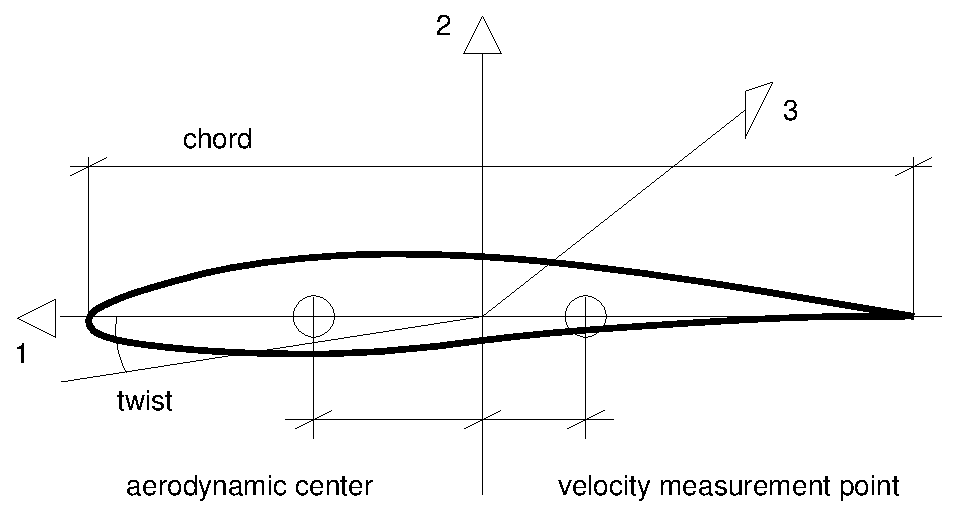
\includegraphics[width=80mm]{airfoil}
  \caption{Airfoil geometry}\label{fig:AIRFOIL}
\end{figure}

The \nt{airfoil\_data} defaults to a built-in NACA 0012 semi-analytical
model (FIXME: the unsteady correction is buggy; use the \kw{c81}
mode instead).

The \kw{multiple} mode of the c81 data allows to specify
more than one airfoil for an aerodynamic element; the transition
between airfoils is sharp.
The integer \nt{airfoil\_number} indicates how many airfoils are expected;
the real \nt{end\_point} indicates where the influence zone for that
airfoil ends, expressed in terms of a non-dimensional abscissa spanning
$\plbr{-1,1}$ along the reference line, roughly along axis 3
of the aerodynamic reference frame; \nt{end\_point} must not lie outside
the element.
So, for example, if airfoil NACA 0015 is used in the leftmost part
of an element up to 1/4 span, NACA 0012 is used from 1/4 to 3/4 span,
and NACA 0009 is used in the remaining rightmost 1/4, the syntax is:
\begin{verbatim}
    set: integer naca0015 = 15;
    set: integer naca0012 = 12;
    set: integer naca0009 = 9;
    c81 data: naca0015, "naca0015.c81";
    c81 data: naca0012, "naca0012.c81";
    c81 data: naca0009, "naca0009.c81";
    # beginning of aerodynamic element definition...
        multiple, 3,
            naca0015, -0.5,    # from -1.0 to -0.5
            naca0012,  0.5,    # from -0.5 to  0.5
            naca0009,  1.0,    # from  0.5 to  1.0
    # ...rest of aerodynamic element definition
\end{verbatim}

The \kw{interpolated} mode of the \kw{c81} data allows to specify
a smooth transition between different airfoils inside an element.
The interpolation occurs at the integration points where the
aerodynamic data are required, and it is performed once for all
at the beginning of the analysis.
Since this operation is time consuming, and essentially unnecessary,
the interpolated data can be generated once for all with the utility
\texttt{util/c81merge} once the position of the integration point is known,
and the \kw{multiple} mode can be used to directly provide
the interpolated data to the aerodynamic element.

The \kw{theodorsen} aerodynamic data uses C81 data,
and superimposes Wagner's approximation of the Theodorsen incompressible
unsteady correction of 2D lift and moment coefficients.
It is experimental.

The \nt{extra\_arglist} allows to define the style of the output.
The \kw{std} style (the default), the \kw{Gauss} and the \kw{node}
styles are illustrated in the output section.


\subsubsection{Output}
Aerodynamic elements, both bodies and beams, write their output with file
extension \texttt{.aer}; for each time step the required elements are output.
In any case the label of the element is output first.
Three different formats are available: \kw{std} (the default),
\kw{Gauss} and \kw{node}.

\begin{itemize}
\item[\kw{std}] (or Coefficients at Gauss points):
the output consists in a set of 8 numbers
for each block, that describe data at each Gauss integration point;
multiple blocks for a single element are written on the same line.
The format is:
\begin{itemize}
    \item the angle of attack at that station, in degrees
	(namely, the angle between the component of the airfoil velocity,
	evaluated at the velocity measurement point, that in the airfoil
	plane and a reference line on the airfoil)
    \item the local yaw angle, in degrees
	(namely, the angle whose tangent is the ratio
	between the axial and the inplane components of the airfoil
	velocity)
    \item the local Mach number
    \item the local lift coefficient
    \item the local drag coefficient
    \item the local aerodynamic moment coefficient
    \item a private number
    \item another private number
\end{itemize}
When \kw{aerodynamic beam2} and \kw{aerodynamic beam3} elements are considered,
the output is repeated for each portion of the beam; so, for example,
a two-node beam is split in two portions, so the output
contains $2\times \nt{integration\_points}$ data blocks,
while a three-node beam is split in three portions,
so the output contains $3\times \nt{integration\_points}$ data blocks.

\item[\kw{node}:]
the format is:
\begin{itemize}
    \item the label of the node
    \item the three components of the force applied to the node
    \item the three components of the couple applied to the node
\end{itemize}
When \kw{aerodynamic beam2} and \kw{aerodynamic beam3} elements are considered,
the output is repeated on the same line for each node
the element is connected to.

\item[\kw{Gauss}] (or Forces at Gauss points):
the output consists in the forces and moments
per unit length at each Gauss integration point; the format is:
\begin{itemize}
    \item the direction of the wind velocity relative to the element frame
    \item the lift,
    \item the drag,
    \item and the aerodynamic moment per unit length
\end{itemize}
When \kw{aerodynamic beam2} \and \kw{aerodynamic beam3} elements are considered,
the output is repeated on the same line for each portion of beam.
\end{itemize}



\subsection{Aeromodal Element}
\emph{Note: implemented by Giuseppe Quaranta; documented by Alessandro Scotti.}

\noindent
This element is used to model an aerodynamic modal element,
i.e.\ an unsteady aerodynamic model that inherits the structural
motion from a \htmlref{\kw{modal joint}}{sec:EL:STRUCT:JOINT:MODAL} element.
Its definition is very similar to that of the modal element,
but it also includes some data representing unsteady aerodynamics
in the time domain trough the residualization matrices.
This element is defined as follows:
%\begin{verbatim}
\begin{Verbatim}[commandchars=\\\{\}]
    \bnt{elem_type} ::= \kw{aeromodal}

    \bnt{normal_arglist} ::=
        \bnt{reference_modal_joint} ,
        (\hty{OrientationMatrix}) \bnt{orientation} ,
        \bnt{reference_chord} ,
        \bnt{number_of_aerodynamic_states} ,
        [ \kw{rigid} , ]
        [ \kw{gust} , \bnt{Vff} , ]
        " \bnt{modal_matrices_file} "
\end{Verbatim}
%\end{verbatim}
With this formulation, anytime an \kw{aeromodal} element is defined,
the user needs to declare the number of modal aerodynamic elements
in use in the \kw{control data} section.
An \htmlref{\kw{air properties}}{sec:EL:AERO:AIRPROPERTIES}
card definition is also required.

The label \nt{reference\_modal\_joint} indicates
the \htmlref{\kw{modal joint}}{sec:EL:STRUCT:JOINT:MODAL}
associated with the \kw{aeromodal} element.
The modal joint must be connected to a \kw{modal} node;
clamped modal joints are not supported.

The keyword \kw{rigid} indicates that the generalized aerodynamic forces
provided by the model include global forces and moments associated
to the rigid body motion of the underlying modal element (FIXME: untested).

The keyword \kw{gust} activates an optional gust model,
which is totally undocumented;
for further information, please contact the Author(s).

The \nt{modal\_matrices\_file} file is an ASCII file that contains
the matrices $\T{A}$, $\T{B}$, $\T{C}$, $\T{D}_0$, $\T{D}_1$ and $\T{D}_2$,
of a state space model according to the representation
\begin{align*}
	\dot{\T{x}}
	&=
	\T{A}\T{x} + \T{B}\T{q}
	\\
	\T{f}
	&=
	q\plbr{\T{C}\T{x} + \T{D}_0 \T{q} + \frac{c}{2V_{\infty}} \T{D}_1 \dot{\T{q}} + \plbr{\frac{c}{2V_{\infty}}}^2 \T{D}_2 \ddot{\T{q}}}
\end{align*}
where $\T{x}$ are the \nt{number\_of\_aerodynamic\_states} (\nt{na})
aerodynamic state variables,
$\T{q}$ are the \nt{ns} modal variables that describe the structural motion
as defined in the related \htmlref{\kw{modal joint}}{sec:EL:STRUCT:JOINT:MODAL},
$c$ is the reference length, $V_\infty$ is the free airstream velocity,
$q = \rho V_{\infty}^2/2$ is the dynamic pressure,
and $\T{f}$ are the unsteady aerodynamic forces applied to the structural
dynamics equations.

When the keyword \kw{rigid} is present, the number of modal variables \nt{ns}
includes the modes provided
by the \htmlref{\kw{modal joint}}{sec:EL:STRUCT:JOINT:MODAL}
plus 6 rigid-body modes corresponding to rigid-body displacement
and rotation of the \kw{modal node}.

The file is formatted as follows:
%\begin{verbatim}
\begin{Verbatim}[commandchars=\\\{\}]
    *** MATRIX A
    (\bnt{na} x \bnt{na} coefficients)
    *** MATRIX B
    (\bnt{na} x \bnt{ns} coefficients)
    *** MATRIX C
    (\bnt{ns} x \bnt{na} coefficients)
    *** MATRIX D0
    (\bnt{ns} x \bnt{ns} coefficients)
    *** MATRIX D1
    (\bnt{ns} x \bnt{ns} coefficients)
    *** MATRIX D2
    (\bnt{ns} x \bnt{ns} coefficients)
\end{Verbatim}
%\end{verbatim}

\paragraph{Example.} \
\begin{verbatim}
    aeromodal: WING, WING_JOINT,
        eye,
        131.25, 10, "ha145b.fea";
\end{verbatim}
The \kw{aeromodal} element is declared with the label \texttt{WING}.
This element is attached to a \kw{modal} joint
named \texttt{WING\_JOINT}.
The orientation of the aerodynamic reference with respect
to the nodal reference is here expressed by the identity matrix (\kw{eye}).
The aerodynamic element chord is 131.25 inches.
This quantity must be consistent with the system chosen to define
the whole model (SI, for example; in this case, British Units).
The next field, 10, indicates the number of states needed to use
the aerodynamic model.
\texttt{ha145b.fea} is the name of the file that contains
the state space model matrices, obtained with an approximation
chosen by the user.
In this particular case, a 10 states Pad\'e approximation
has been chosen.
This example is taken from the Bisplinghoff Ashley Halfman
(BAH) Jet Transport Wing cantilevered wing with modal aerodynamic
frequency response, computed by a double-lattice method at Mach 0.0.
Data were extracted from the MSC-NASTRAN aeroelastic example file,
named \texttt{ha145b}, while the aerodynamic state-space fitting
has been computed using a Pad\'e polynomial approximation
(by Pasinetti \& Mantegazza, \cite{PASINETTI-MANTEGAZZA-1999}).
All quantities are expressed in inches and pounds.



\subsection{Aircraft Instruments}
%\begin{verbatim}
\begin{Verbatim}[commandchars=\\\{\}]
    \bnt{elem_type} ::= \kw{aircraft instruments}

    \bnt{normal_arglist} ::= \bnt{aircraft_node}
        [ , \kw{orientation} , \{ \kw{flight mechanics} | \kw{aeroelasticity}
            | (\hty{OrientationMatrix}) \bnt{relative_orientation} \} ]
	    [ , \kw{initial latitude} , (\ty{real})\bnt{initial_latitude}  \} ]
	    [ , \kw{initial longitude} , (\ty{real})\bnt{initial_longitude}  \} ]
	    [ , \kw{earth radius} , (\ty{real})\bnt{earth_radius}  \} ]
\end{Verbatim}
%\end{verbatim}
The \nt{aircraft\_node} represents the aircraft; it is assumed
that the positive $x$ direction of the node is tail to nose of the aircraft,
the positive $z$ direction of the node is top to bottom of the aircraft,
and the positive $y$ direction of the node is to the right of the pilot.
The node representing the aircraft is intended in a ``world''
reference frame whose positive $z$ direction points upward
and whose positive $x$ direction points north
(note that currently the world is flat).

An optional orientation can be added to change the orientation
of the aircraft with respect to the node.
This is useful, for example, with aeroelasticity, in which conventionally
the positive direction of the $x$ axis is nose to tail,
and the positive direction of the $z$ axis is bottom to top.
The keyword \kw{flight mechanics} indicates that the node representing
the aircraft is oriented according to the default orientation
of the element, whereas the keyword \kw{aeroelasticity}
indicates that the node representing the aircraft is oriented accordingly.
Arbitrary orientations can be dealt with by providing an appropriate
\nt{relative\_orientation} matrix.

Values for the initial latitude and longitude can be provided, in
radians. If not set, they are supposed null at the initial time. Also
the earth radius can optionally be provided, with the default value
being the average, \textbf{6371005 m}.

Please note that longitude and latitude are calculated assuming a ``flat''
world, discarding the Earth's surface curvature.

\begin{center}
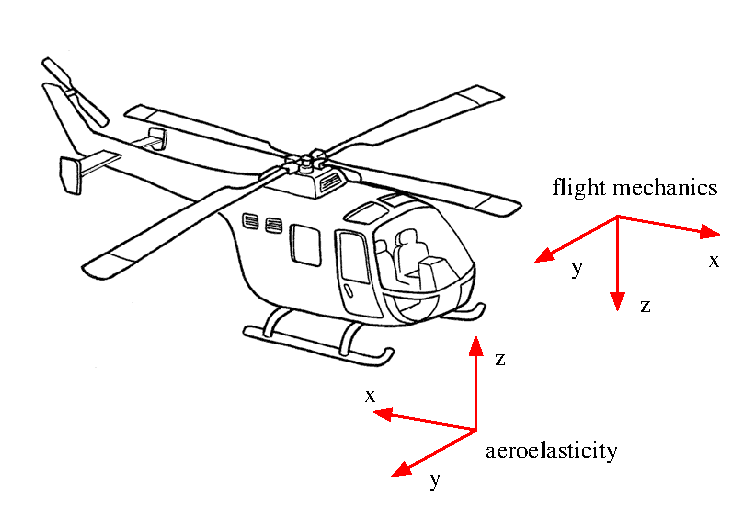
\includegraphics[width=.5\textwidth]{elicottero}
\end{center}

The available measures are accessed during the simulation
by defining appropriate \kw{parameter} nodes, and by binding
the \kw{aircraft instruments} element private data to the nodes
by means of the \kw{bind} mechanism, or directly by means
of the
\hyperref{\kw{element} drive}{\kw{element} drive (see Section~}{)}{sec:DriveCaller:ELEMENT}.

\paragraph{Private Data}
The following data are available:
\begin{itemize}
\item \kw{"airspeed"}: the airspeed as seen by the reference
	point on the aircraft, i.e.\ the absolute value
	of the combination of the airstream speed and of the node speed,
  with units m/s
\item \kw{"groundspeed"}: the absolute value of the projection
	of the node speed in the $xy$ plane of the ``world'', with units m/s
\item \kw{"altitude"}: the $z$ component of the node position
	with respect to the ``world'', in meters
\item \kw{"attitude"}: the angle between the $x$ axis of the local
  frame and the ``world'' $xy$ plane,  i.e. $\sin^{-1}\plbr{r_{31}}$,
  in radians
\item \kw{"bank"}: the angle between the $y$ axis of the local
	frame and the ``world'' $xy$ plane, i.e. $\sin^{-1}\plbr{r_{32}}$,
  in radians
\item \kw{"turn"}: the turn rate, the $z$ component of the angular
  velocity expressed in the ``world'' reference frame, measured in rad/min
\item \kw{"slip"}: the sideslip angle, the angle between the $x$ axis of
  the local frame and the projection of the velocity vector in the $xy$
  plane of the local frame, units are radians (also \kw{"sideslip"})
\item \kw{"verticalspeed"}: the $z$ component of the node velocity
	in the ``world'' reference system, in m/s
\item \kw{"angleofattack"}: the angle between the local $z$ and $x$ components
	of the velocity (airstream plus node), expressed in the reference frame
  of the aircraft, in radians (also \kw{"aoa"})
\item \kw{"heading"}: the angle between the $x$ axis of the aircraft
	and the ``north'' (the global $x$ axis) about the global $z$ axis,
  in radians
\item \kw{"longitude"}: the aicraft longitude, in radians
\item \kw{"latitude"}: the aicraft latitude, in radians
\item \kw{"rollrate"}: the component of the angular velocity
	of the node representing the aircraft along the $x$ axis
	of the node itself (positive when the right wing moves downward),
  in rad/s
\item \kw{"pitchrate"}: the component of the angular velocity
	of the node representing the aircraft along the $y$ axis
	of the node itself (positive when the nose pitches upward),
  in rad/s
\item \kw{"yawrate"}: the component of the angular velocity
	of the node representing the aircraft along the $z$ axis
	of the node itself (positive when the right wing moves backward),
  in rad/s
\end{itemize}
Additional data, not available through usual aircraft instruments, are available:
\begin{itemize}
\item \kw{"init\_x1"}: $x$ component of initial position, in absolute frame
\item \kw{"init\_x2"}: $y$ component of initial position, in absolute frame
\item \kw{"init\_longitude"}: initial longitude
\item \kw{"init\_latitude"}: initial latitude
\item \kw{"body\_axb"}: $x$ component of linear acceleration, in body frame
\item \kw{"body\_ayb"}: $y$ component of linear acceleration, in body frame
\item \kw{"body\_azb"}: $z$ component of linear acceleration, in body frame
\item \kw{"body\_pd"}: $x$ component of pitch angular acceleration, in body frame
\item \kw{"body\_qd"}: $y$ component of pitch angular acceleration, in body frame
\item \kw{"body\_rd"}: $z$ component of pitch angular acceleration, in body frame
\item \kw{"body\_vx"}: $x$ component of air speed, in body frame
\item \kw{"body\_vy"}: $y$ component of air speed, in body frame
\item \kw{"body\_vz"}: $z$ component of air speed, in body frame
\item \kw{"density"}: density at the body's altitude
\item \kw{"soundcelerity"}: sound celerity at the body's altitude
\item \kw{"staticpressure"}: static pressure at the body's altitude
\item \kw{"temperature"}: temperature at the body's altitude
\end{itemize}

\paragraph{Example.} \
\begin{verbatim}
    # expose heading using a parameter node
    # ...
    structural: AIRCRAFT, dynamic, ...
    parameter: HEADING, /* bound to */ element;
    # ...
    aircraft instruments: AIRCRAFT, AIRCRAFT, orientation, aeroelasticity;
    bind: AIRCRAFT, aircraft instruments, HEADING, string, "heading";

    # implement a minimal SCAS on roll & yaw
    # ...
    structural: AIRCRAFT, dynamic, ...
    # ...
    aircraft instruments: AIRCRAFT, AIRCRAFT, orientation, flight mechanics;
    couple: AIRCRAFT, follower,
        AIRCRAFT,
            position, null,
            component,
                element, AIRCRAFT, aerodynamic element, string, "rollrate",
                    linear, 0., -ROLL_GAIN,
                0.,
                element, AIRCRAFT, aerodynamic element, string, "yawrate",
                    linear, 0., -YAW_GAIN;
\end{verbatim}




\subsection{Air Properties}\label{sec:EL:AERO:AIRPROPERTIES}
The properties of the airstream are made of the physical properties
of the air plus the description of the airstream velocity direction
and amplitude.
The former can be expressed in different forms, while the latter
are based on three-dimensional drive callers, \htybty{TplDriveCaller}{Vec3}.
%\begin{verbatim}
\begin{Verbatim}[commandchars=\\\{\}]
    \bnt{elem_type} ::= \kw{air properties}

    \bnt{arglist} ::=
        \{ (\hty{DriveCaller}) \bnt{air_density} , (\ty{real}) \bnt{sound_celerity}
            | \kw{std} , \{ \{ \kw{SI} | \kw{British} \}
                [ , \kw{temperature deviation} , \bnt{delta_T} ]
                | \bnt{p0} , (\hty{DriveCaller}) \bnt{rho0} ,
                    \bnt{T0} , \bnt{dT/dz} , \bnt{R} , \bnt{g0} , \bnt{z1} , \bnt{z2} \}
            [ , \kw{reference altitude} , \bnt{z0} ] \} ,
        (\htybty{TplDriveCaller}{Vec3}) \bnt{air_speed}
        [ , \kw{gust} , \bnt{gust_model} [ , ... ] ]
\end{Verbatim}
%\end{verbatim}
The first form consists in the bare input of the air density,
in form of a drive caller, and of the sound celerity, e.g.:
\begin{verbatim}
    air properties: 1.225, 340.,
        1.,0.,0., 150.;
\end{verbatim}
The second form uses standard air properties, both in the
international system (SI) or in British units.
A temperature deviation and an altitude offset can be defined, e.g.:
\begin{verbatim}
    air properties: std, SI, temperature deviation, -55,
        reference altitude, 1000.,
        1.,0.,0., 150.;
\end{verbatim}
where standard properties in SI are used, with a temperature
deviation of -55 K and a reference altitude of 1000 m.
The air properties are computed based on the $z$ position of the
point where the \kw{air properties} are requested (plus the optional
altitude offset).
The last possibility lets the user input all the parameters
required to compute the \kw{air properties} based on the $z$ position
of the point where they are requested, namely the reference
pressure \nt{p0}, the reference density \nt{rho0},
the reference temperature \nt{T0}, the initial temperature
gradient \nt{dT/dz}, the gas constant \nt{R}, the
initial gravity acceleration \nt{g0}, the bottom and top
altitudes of the null temperature gradient region \nt{z1} and
\nt{z2}; e.g., for SI units:
\begin{verbatim}
    air properties: std,
        101325.,       /* Pa, 1 bar */
        1.2250,        /* kg/m^3 */
        288.16,        /* K, ISA: 15 C */
        -6.5e-3,       /* K/m */
        287.,          /* J/kgK */
        9.81,          /* m/s^2 */
        11000.,        /* m */
        25000.,        /* m */
        temperature deviation, -55,
        reference altitude, 1000.,
        1.,0.,0., 150.;
\end{verbatim}
The air properties are defined according to the formulas
\begin{subequations}
\begin{align}
	\rcubr{\lvvect{
		T = \nt{T0} + \nt{dT/dz} \cdot z
		\\
		p = \nt{p0} \plbr{\cfrac{T}{\nt{T0}}}^{-\frac{\nt{g0}}{\nt{dT/dz} \cdot \nt{R}}}
		\\
		\rho = \nt{rho0} \plbr{\cfrac{T}{\nt{T0}}}^{-\plbr{\frac{\nt{g0}}{\nt{dT/dz} \cdot \nt{R}} + 1}}
	}}
	&&& z < \nt{z1}
	\\
	\rcubr{\lvvect{
		T = \nt{T0} + \nt{dT/dz} \cdot \nt{z1}
		\\
		p = \plbr{\nt{p0}\plbr{\cfrac{T}{\nt{T0}}}^{-\frac{\nt{g0}}{\nt{dT/dz} \cdot \nt{R}}}}
			\mathrm{e}^{-\nt{g0} \frac{z - \nt{z1}}{\nt{dT/dz} \cdot \nt{R}}}
		\\
		\rho = \nt{rho0} \plbr{\cfrac{T}{\nt{T0}}}^{-\plbr{\frac{\nt{g0}}{\nt{dT/dz} \cdot \nt{R}} + 1}}
			\mathrm{e}^{-\nt{g0} \frac{z - \nt{z1}}{\nt{dT/dz} \cdot \nt{R}}}
	}}
	&&& \nt{z1} \le z < \nt{z2}
\end{align}
\end{subequations}
The case of $z > \nt{z2}$ is not currently handled;
the formulas for $z \ge \nt{z1}$ are actually used.
The value of $z$ is computed by adding the $z$ component
of the position where the air properties are computed
to the reference altitude \nt{z0}.

The asymptotic air properties are characterized by \nt{air\_speed},
the \htybty{TplDriveCaller}{Vec3} of the air speed,
expressed in the global reference frame.
The possibility to vary the density and the airspeed using a driver
has little physical meaning, especially the former;
is intended as a practical means to gradually introduce
the desired air properties, and the related airloads, in the analysis.

\subsubsection{Gust}
If the optional \kw{gust} keyword is used, a gust model can be added.
Note that a very elementary gust model, represented by a uniform change
in airstream speed and direction can be implemented by using
a time-dependent airstream drive.

Gusts can also be appended later to the \kw{air properties} element
by using the statement
%\begin{verbatim}
\begin{Verbatim}[commandchars=\\\{\}]
    \kw{gust} : \bnt{gust_model} ;
\end{Verbatim}
%\end{verbatim}


\paragraph{Front 1D Gust}
The syntax of the \kw{front 1D} gust model is:
%\begin{verbatim}
\begin{Verbatim}[commandchars=\\\{\}]
    \bnt{gust_model} ::= \kw{front 1D} ,
        (\hty{Vec3})        \bnt{front_direction} ,
        (\hty{Vec3})        \bnt{perturbation_direction} ,
        (\ty{real})      \bnt{front_velocity} ,
        (\hty{DriveCaller}) \bnt{front_profile}
\end{Verbatim}
%\end{verbatim}
This model consists in a uniform front, defined as
\begin{displaymath}
	\T{v}\plbr{\T{x}, t} = \T{n} g\plbr{V_\mathrm{ref} \cdot t - \T{f} \cdot \T{x}}
\end{displaymath}
where
\begin{itemize}
\item $\T{v}$ is the velocity perturbation in the global frame;
\item $\T{x}$ is the position, in the global frame, of the point whose airstream velocity
is being evaluated;
\item $t$ is the current time;
\item $\T{n}$ is the unit vector \nt{perturbation\_direction}
that defines the direction of the velocity perturbation in the global frame;
\item $g\plbr{\cdot}$ is the function \nt{front\_profile}
that defines the gust profile as a function of $x = V_\mathrm{ref} \cdot t - \T{f} \cdot \T{x}$, i.e., the local position (in units of length) of the measure point in a frame moving with the gust front along the $\T{f}$ direction;
\item $\T{f}$ is the unit vector \nt{front\_direction}
that defines the direction of propagation of the front in the global frame;
\item $V_\mathrm{ref}$ is the constant velocity \nt{front\_velocity}
of propagation of the front in direction $\T{f}$.
\end{itemize}
As an example, a transverse cosine-shaped gust, with a wavelength of 100 m
and a peak velocity of 5 m/s moving downstream at the airstream speed,
100 m/s, in standard air, starting along axis $x$ of the global frame at $-200$ m with respect to the origin of the global frame, is presented:
\begin{verbatim}
    set: real waveLength = 100.; # m
    set: real V_inf = 100.;      # m/s
    set: real V_g = 5.;          # m/s
    set: real x_0 = -200;         # m, position of the gust's local frame at Time = 0.
    air properties: std, SI,
        1.,0.,0., const, V_inf,  # reference airstream along X
        gust, front 1D,
            1.,0.,0.,            # front moving along X
            0.,0.,1.,            # gust along Z
            V_inf,               # front moving at V_inf
            cosine, -x_0, pi/waveLength, V_g/2., one, 0.;
            # step, -x_0, V_g, 0.;
\end{verbatim}
% set: real T_0 = 2;           # s, time at which the gust origin passes from the global origin
% cosine, V_inf*T_0, pi/waveLength, V_g/2., one, 0.;



\paragraph{Scalar Function Wind Profile}
The syntax of the \kw{scalar function} wind profile,
implemented as a gust model within the \kw{air properties}, is:
%\begin{verbatim}
\begin{Verbatim}[commandchars=\\\{\}]
    \bnt{gust_model} ::= \kw{scalar function} ,
        \kw{reference position} , (\hty{Vec3}) \bnt{X0} ,
        \kw{reference orientation} , (\hty{OrientationMatrix}) \bnt{R0} ,
        (\hty{ScalarFunction}) \bnt{sf}
\end{Verbatim}
%\end{verbatim}
It yields a uniform velocity profile along the $x$ axis of the
reference orientation as a function of the $z$ axis component
of the relative position; namely, given the relative position
\begin{align}
	z &= \T{e}_3 \cdot \plbr{\T{x} - \nt{X0}}
	,
\end{align}
the velocity is
\begin{align}
	\T{v}
	&=
	\T{e}_1 \cdot \nt{sf}(z)
	,
\end{align}
where $\T{e}_i$ is the $i$-th axis of the reference orientation \nt{R0}.



\paragraph{Power Law Wind Profile}
The syntax of the \kw{power law} wind profile, implemented as a gust model
within the \kw{air properties}, is:
%\begin{verbatim}
\begin{Verbatim}[commandchars=\\\{\}]
    \bnt{gust_model} ::= \kw{power law} ,
        \kw{reference position} , (\hty{Vec3}) \bnt{X0} ,
        \kw{reference orientation} , (\hty{OrientationMatrix}) \bnt{R0} ,
        \kw{reference elevation} , \bnt{z_ref} ,
        \kw{reference velocity} , (\hty{DriveCaller}) \bnt{v_ref} ,
        \kw{exponent} , \bnt{exponent}
\end{Verbatim}
%\end{verbatim}
It yields a uniform velocity profile along the $x$ axis of the
reference orientation as a function of the $z$ axis component
of the relative position; namely, given the relative position
\begin{align}
	z &= \T{e}_3 \cdot \plbr{\T{x} - \nt{X0}}
	,
\end{align}
the velocity is
\begin{align}
	\T{v}
	&=
	\T{e}_1 \cdot \nt{v\_ref} \plbr{\frac{z}{\nt{z\_ref}}}^{\nt{exponent}}
	,
\end{align}
where $\T{e}_i$ is the $i$-th axis of the reference orientation \nt{R0}.
Typical values of \nt{exponent} are about 0.1.



\paragraph{Logarithmic Wind Profile}
The syntax of the \kw{logarithmic} wind profile, implemented as a gust model
within the \kw{air properties}, is:
%\begin{verbatim}
\begin{Verbatim}[commandchars=\\\{\}]
    \bnt{gust_model} ::= \kw{logarithmic} ,
        \kw{reference position} , (\hty{Vec3}) \bnt{X0} ,
        \kw{reference orientation} , (\hty{OrientationMatrix}) \bnt{R0} ,
        \kw{reference elevation} , \bnt{z_ref} ,
        \kw{reference velocity} , (\hty{DriveCaller}) \bnt{v_ref} ,
        \kw{surface roughness length} , \bnt{z_0}
\end{Verbatim}
%\end{verbatim}
It yields a uniform velocity profile along the $x$ axis of the
reference orientation as a function of the $z$ axis component
of the relative position; namely, given the relative position
\begin{align}
	z &= \T{e}_3 \cdot \plbr{\T{x} - \nt{X0}}
	,
\end{align}
the velocity is
\begin{align}
	\T{v}
	&=
	\T{e}_1 \cdot \nt{v\_ref} \cdot \frac{
		\log(z/\nt{z\_0}) - \psi_m
	}{
		\log(\nt{z\_ref}/\nt{z\_0}) - \psi_m
	}
	,
\end{align}
where $\T{e}_i$ is the $i$-th axis of the reference orientation \nt{R0}.

The surface roughness length describes the typical roughness
of the surrounding surface.
It is a very small number in case of smooth surface
(e.g.\ 0.01m for grass),
or 1/20 to 1/30 of the typical obstacle's size (e.g.\ 1m for woods).


\paragraph{Output}
The output occurs in the \texttt{.air} file, which contains:
\begin{itemize}
\item a fake label, always set to 1
\item the air density
\item the sound celerity
\item the three components of the reference air speed
with respect to the inertial reference frame
\end{itemize}


\paragraph{Private Data}
The following data are available:
\begin{itemize}
\item \kw{"vxinf"} the $x$ component of the airstream speed (without any gust contribution)
\item \kw{"vyinf"} the $y$ component of the airstream speed (without any gust contribution)
\item \kw{"vzinf"} the $z$ component of the airstream speed (without any gust contribution)
\item \kw{"vinf"} the module of the airstream speed (without any gust contribution)
\end{itemize}



\subsection{Generic Aerodynamic Force}
\label{sec:EL:AERO:GAF}
This element computes generalized aerodynamic forces parametrized
on dynamic pressure and angle of attack and sideslip angle.
%\begin{verbatim}
\begin{Verbatim}[commandchars=\\\{\}]
    \bnt{elem_type} ::= \kw{generic aerodynamic force}

    \bnt{normal_arglist} ::= \bnt{node_label} ,
        [ \kw{position} , \bnt{relative_position} , ]
        [ \kw{orientation} , \bnt{relative_orientation} , ]
        [ \kw{reference surface} , \bnt{reference_surface} , ]
        [ \kw{reference length} , \bnt{reference_length} , ]
        [ \kw{alpha first} , \{ \kw{no} | \kw{yes} \} , ]
        \{ \bnt{data_file_specification} | \kw{reference} , \bnt{gaf_data_label} \}

    \bnt{data_file_specification} ::= \kw{file} ,
        [ \{ \kw{angle units} , \{ \kw{radians} | \kw{degrees} \}
            | \kw{scale angles} , \bnt{angle_scale_factor} \} , ]
        [ \kw{scale lengths} , \bnt{length_scale_factor} , ]
        " \bnt{data_file_name} "
\end{Verbatim}
%\end{verbatim}
This element computes aerodynamic forces and moments $\T{f}_a$, $\T{m}_a$
proportional to the dynamic pressure $q=\rho \T{v}^T \T{v}/2$
and to empirical coefficients tabulated as functions
of the angle of attack $\alpha$ and the sideslip angle $\beta$.
The angles are computed from the relative airstream velocity $\T{v}$
expressed in the reference frame of the body.
The velocity is computed at the reference point, optionally offset
from the node \nt{node\_label} by the offset \nt{relative\_position}
(defaults to \kw{null}), in a reference frame optionally oriented
from that of the node \nt{node\_label} by the orientation matrix
\nt{relative\_orientation} (defaults to \kw{eye}), namely
\begin{subequations}
\begin{align}
	\TT{o} &= \text{(\hty{Vec3})} \ \nt{relative\_position}
	\\
	\TT{R}_h &= \text{(\hty{OrientationMatrix})}\ \nt{relative\_orientation}
	\\
	\TT{v} &= \TT{R}_h^T \TT{R}_n^T \plbr{
		\dot{\T{x}}_n + \T{\omega}_n \times \TT{R}_n \TT{o}
	}
	,
\end{align}
\end{subequations}
where $\T{x}_n$ and $\TT{R}_n$ are the position and orientation
of the node, and $\dot{\T{x}}_n$ and $\T{\omega}_n$ are its linear
and angular velocity.
By default the angles are computed from the components of $\T{v}$
according to the formulas
\begin{subequations}
\begin{align}
	\alpha
	&=
	\text{atan}\plbr{
		\cfrac{v_3}{\nrbr{v_1}}
	}
	\\
	\beta
	&=
	-\text{atan}\plbr{
		\cfrac{v_2}{\text{sign}(v_1)\sqrt{v_1^2 + v_2^2}}
	}
	;
\end{align}
\end{subequations}
as a consequence, $-\pi/2 \le \alpha \le \pi/2$
and $-\pi \le \beta \le \pi$.
If the optional keyword \kw{alpha first} is set to \kw{yes},
the alternative formulas
\begin{subequations}
\begin{align}
	\alpha
	&=
	\text{atan}\plbr{
		\cfrac{v_3}{\text{sign}(v_1)\sqrt{v_1^2 + v_2^2}}
	}
	\\
	\beta
	&=
	-\text{atan}\plbr{
		\cfrac{v_2}{\nrbr{v_1}}
	}
	.
\end{align}
\end{subequations}
are used; as a consequence, $-\pi \le \alpha \le \pi$
and $-\pi/2 \le \beta \le \pi/2$.
In both cases, they assume that the body reference system
is loosely aligned as:
\begin{itemize}
\item axis 1 goes from tail to nose of the aircraft;
\item axis 2 points ``to the right'';
\item axis 3 points towards the ground when the aircraft is in level flight.
\end{itemize}
Force and moment are consistently applied to the node as
\begin{subequations}
\begin{align}
	\T{f}_n &= \TT{R}_n \TT{R}_h \T{f}_a
	\\
	\T{m}_n &= \T{R}_n \TT{R}_h \TT{m}_a
		+ \TT{R}_n \plbr{\T{o} \times \plbr{\TT{R}_h \T{f}_a}}
\end{align}
\end{subequations}

\emph{Note: this element does not contribute to the Jacobian matrix
of the problem; as such, it may deteriorate the convergence properties
of the solution when aerodynamic forces dominate the problem.
Moreover, it is not suitable for the direct computation of the eigenvalues
of a problem about a steady solution.}

\emph{Note: this element, by itself, may not be adequate to model
the rigid body aerodynamics of an aircraft, since it does not
account for the dependence of force and moment on angle rates.}

\paragraph{Output}
The following output is available:
\begin{enumerate}
\item column 1: element label
\item column 2: the angle of attack $\alpha$
\item column 3: the sideslip angle $\beta$
\item columns 4--6: the components of force $\T{f}_a$
	in local $x$, $y$ and $z$ directions
\item columns 7--9: the components of moment $\T{m}_a$
	in local $x$, $y$ and $z$ directions,
	about the reference point (node plus offset)
\item columns 10--12: the components of force $\T{f}_n$
	in global $x$, $y$ and $z$ directions
\item columns 13--15: the components of moment $\T{m}_n$
	in global $x$, $y$ and $z$ directions,
	about the node
\end{enumerate}

\paragraph{Private Data}
The \kw{generic aerodynamic force} element outputs the following private data:
\begin{itemize}
\item \kw{"Fx"}, \kw{"Fy"}, \kw{"Fz"}:
	force components in the global reference frame;

\item \kw{"Mx"}, \kw{"My"}, \kw{"Mz"}:
	moment components in the global reference frame, about the node;

\item \kw{"fx"}, \kw{"fy"}, \kw{"fz"}:
	force components in the local reference frame;

\item \kw{"mx"}, \kw{"my"}, \kw{"mz"}:
	moment components in the local reference frame, about the reference point;

\item \kw{"alpha"}: angle of attack (in radian)

\item \kw{"beta"}: sideslip angle (in radian)
\end{itemize}
The values computed during the last residual assembly are returned.

\subsubsection{Generic Aerodynamic Element Data}
Data is stored in ASCII format in a file.

An arbitrary number of comment lines is allowed at the beginning.
Comment lines start with either a percent `\textbf{\%}'
or a hash mark `\texttt{\#}' in the first column.
Their content is discarded until the end of the line.

The first non-comment line must contain two integers separated by whitespace.
The integers represent the expected number of angle of attack
and sideslip angle values, $N_\alpha$ and $N_\beta$.

Another arbitrary number of comment lines is allowed.

A set of $N_\alpha \cdot N_\beta$ lines is expected.
No comments or empty lines are allowed in between.
Each line contains:
\begin{itemize}
\item column 1: the angle of attack, $\alpha$
\item column 2: the sideslip angle, $\beta$
\item columns 3--5: the force coefficients $f_{x/q}$, $f_{y/q}$, $f_{z/q}$
\item columns 6--8: the moment coefficients $m_{x/q}$, $m_{y/q}$, $m_{z/q}$
\end{itemize}

Notes:
\begin{enumerate}
\item lines are sorted as follows:
all values of $\alpha$ are defined for each value of $\beta$;
the same values of $\alpha$ are expected for each value of $\beta$;
\item the angle ranges are $-\pi/2 \le \alpha \le \pi/2$ and
$-\pi \le \beta \le \pi$; or, if \kw{alpha first} is \kw{yes},
they are $-\pi \le \alpha \le \pi$ and $-\pi/2 \le \beta \le \pi/2$;
\item the angles are expected in radians;
use the mutually exclusive optional keywords \kw{angle units},
to specify either \kw{radians} or \kw{degrees},
or \kw{scale angles}, to specify the \nt{angle\_scale\_factor}.
The \nt{angle\_scale\_factor} is the factor that when multiplied by the
angle transforms it into radians; for example, if angles are provided
in degrees then $\nt{angle\_scale\_factor} = \pi/180$;
\item $q=1/2 \rho V^2$ is the local reference dynamic pressure,
where $V$ is the norm of the velocity at the reference point;
\item the coefficients express forces and moments in the reference frame
attached to the body;
\item the coefficients are either expected in dimensional
or non-dimensional form.
In the former case, the force coefficients represent areas,
while the moment coefficients represent volumes, since they need
to be multiplied by the dynamic pressure to become forces and moments.
In the latter case, they are pure numbers; a \nt{reference\_surface}
and \nt{reference\_length} must be defined in the configuration
of the corresponding \kw{generic aerodynamic force} element.
When dimensional coefficients are specified, they can be rescaled
by using the optional keyword \kw{scale lengths} to specify
the \nt{length\_scale\_factor}.
\end{enumerate}

\paragraph{Example.}
The content of the file \texttt{example.dat} is
\begin{verbatim}
# This is an example of data for the "generic aerodynamic force" element
# 5 values of angle of attack (alpha) and 4 values of sideslip angle (beta)
# are provided
5 4
# alpha beta fx/q fy/q fz/q mx/q my/q mz/q
-90 -180  0  0  0  0  0  0
-20 -180  0  0  0  0  0  0
  0 -180  0  0  0  0  0  0
 20 -180  0  0  0  0  0  0
 90 -180  0  0  0  0  0  0
-90  -20  0  0  0  0  0  0
-20  -20  0  0  0  0  0  0
  0  -20  0  0  0  0  0  0
 20  -20  0  0  0  0  0  0
 90  -20  0  0  0  0  0  0
-90   20  0  0  0  0  0  0
-20   20  0  0  0  0  0  0
  0   20  0  0  0  0  0  0
 20   20  0  0  0  0  0  0
 90   20  0  0  0  0  0  0
-90  180  0  0  0  0  0  0
-20  180  0  0  0  0  0  0
  0  180  0  0  0  0  0  0
 20  180  0  0  0  0  0  0
 90  180  0  0  0  0  0  0
\end{verbatim}
The corresponding statement in the input file is
\begin{verbatim}
    set: integer GAF_NODE = 10;
    set: integer GAF_ELEM = 20;
    generic aerodynamic force: GAF_ELEM, GAF_NODE,
        file, angle units, degrees, "example.dat";
\end{verbatim}



\subsection{Induced velocity}
\label{sec:EL:AERO:INDVEL}
The \kw{induced velocity} element is used to associate the aerodynamic elements
that model the lifting surfaces of an aircraft,
or the blades of a helicopter rotor, when some inflow related computations
are required.

By means of different inflow models, and by means
of the aerodynamic load contributions supplied by the aerodynamic elements,
the \kw{induced velocity} element is able to compute the induced velocity
at an arbitrary point on the lifting surface or rotor disk.
This velocity term in turn is used by the aerodynamic elements to determine
a better estimate of the boundary conditions.

The syntax of the \kw{induced velocity} elements is:
%\begin{verbatim}
\begin{Verbatim}[commandchars=\\\{\}]
    \bnt{elem_type} ::= \kw{induced velocity}

    \bnt{normal_arglist} ::= \bnt{induced_velocity_type} , \bnt{induced_velocity_data}
\end{Verbatim}
%\end{verbatim}

\subsubsection{Rotor}
\label{sec:EL:AERO:INDVEL:ROTOR}
Currently, induced velocity models are only implemented
for helicopter and cycloidal rotors.
For the latter, see Section~\ref{sec:MODULES:CYCLOCOPTER}.
Originally, this type of element was known as \kw{rotor},
and the original syntax is preserved for backwards compatibility.

The syntax of the helicopter rotor \kw{induced velocity} element is:
%\begin{verbatim}
\begin{Verbatim}[commandchars=\\\{\}]
    \bnt{induced_velocity_type} ::= \kw{rotor}

    \bnt{induced_velocity_data} ::= \bnt{craft_node} ,
            [ \kw{orientation} , (\hty{OrientationMatrix}) \bnt{rotor_orientation} , ]
        \bnt{rotor_node} ,
        \kw{induced velocity} , \bnt{induced_velocity_model}
\end{Verbatim}
%\end{verbatim}
The optional \nt{rotor\_orientation} is required when axis 3
of the \nt{craft\_node} is not aligned with the rotor axis; axis 3
of the \nt{rotor\_node} must be aligned with the rotor axis.

There are five models of induced velocity.
The first is no induced velocity; the syntax is:
%\begin{verbatim}
\begin{Verbatim}[commandchars=\\\{\}]
    \bnt{induced_velocity_model} ::= \kw{no}
\end{Verbatim}
%\end{verbatim}
There is no argument list. This element does not compute any induced
velocity, but still computes the rotor traction for output purposes,
if output is required.
The others have a fairly common syntax.  The first three are
\kw{uniform}, \kw{glauert} and \kw{mangler} induced velocity
models:
%\begin{verbatim}
\begin{Verbatim}[commandchars=\\\{\}]
    \bnt{induced_velocity_model} ::=
        \{ \kw{uniform} | \kw{glauert} [ , \kw{type} , \bnt{glauert_type} ] | \kw{mangler} \} ,
        \bnt{reference_omega} , \bnt{reference_radius}
        [ , \bnt{option} [ , ... ] ]

    \bnt{glauert_type} ::= \{ \kw{glauert} | \kw{coleman} | \kw{drees}
        | \kw{payne} | \kw{white and blake} | \kw{pitt and peters} | \kw{howlett} \}

    \bnt{option} ::=
        \{ \kw{ground} , \bnt{ground_node}
            | \kw{delay} , (\hty{DriveCaller}) \bnt{memory_factor}
            | \kw{max iterations} , \bnt{max_iterations}
            | \kw{tolerance} , \bnt{tolerance}
            | \kw{eta} , \bnt{eta}
            | \kw{correction} , \bnt{hover_correction_factor}, \bnt{ff_correction_factor} \}
\end{Verbatim}
%\end{verbatim}

\begin{itemize}
\item
The \nt{reference\_omega} field is used to decide whether
the induced velocity computation must be inhibited because the rotor speed
is very low.

\item
The \nt{reference\_radius} field is used to make the rotor related parameters
non-dimensional.

\item
The \kw{ground} parameter is used to inform the rotor about the proximity
to the ground; the $z$ component of the distance between the rotor
and the ground nodes, in the ground node reference frame
(direction 3, positive),
is used for an approximate correction of the axial inflow velocity
\cite{NASA-TR-3021}.

\item
The \nt{memory\_factor}, the \nt{hover\_correction\_factor}
and the \nt{ff\_correction\_factor} (forward flight) are
used to correct the nominal induced velocity, according to the formula
\begin{align*}
	U_{\text{effective}}
	&=
	\plbr{1 - \nt{memory\_factor}} U_{\text{nominal}}
	\\
	&+ \nt{memory\_factor} \ U_{\text{previous}}
\end{align*}
with
\begin{align*}
	U_{\text{nominal}}
	&=
	\frac{T}{2 \rho A V_{\text{tip}} \sqrt{
		\cfrac{\lambda^2}{\nt{hover\_correction\_factor}^4}
		+ \cfrac{\mu^2}{\nt{ff\_correction\_factor}^2}
	}}
\end{align*}
The \kw{delay} parameter is used to linearly combine the current
reference induced velocity with the induced velocity at the previous step;
no delay means there is no memory of the previous value.
The memory factor behaves like a discrete first-order low-pass filter.
As a consequence, its behavior depends on the integration time step.
The \nt{memory\_factor} parameter defaults to 0.
The \nt{hover\_correction\_factor}
and \nt{ff\_correction\_factor} parameters default to 1.

\item
The \nt{max\_iterations}, \nt{tolerance}
and \nt{eta} parameters refer to the iteration cycle
that is performed to compute the nominal induced velocity.
After \nt{max\_iterations}, or when the absolute value
of the difference between two iterations of the nominal induced
velocity is less than \nt{tolerance}, the cycle ends.
Only a fraction \nt{eta} of the difference between two
iterations of the nominal induced velocity is actually
used; \nt{eta} defaults to 1.
The default is to make only one iteration, which is backward-compatible
with the original behavior.
\end{itemize}

The last induced velocity model uses a dynamic inflow model,
based on \cite{PITT}, with 3 inflow states.
The syntax is:
%\begin{verbatim}
\begin{Verbatim}[commandchars=\\\{\}]
    \bnt{induced_velocity_model} ::= \kw{dynamic inflow} ,
        \bnt{reference_omega} ,
        \bnt{reference_radius}
        [ , \bnt{option} [ , ... ] ]

    \bnt{option} ::=
        \{ \kw{ground} , \bnt{ground_node}
            | \kw{initial value} , \bnt{const_vel} , \bnt{cosine_vel} , \bnt{sine_vel}
            | \kw{max iterations} , \bnt{max_iterations}
            | \kw{tolerance} , \bnt{tolerance}
            | \kw{eta} , \bnt{eta}
            | \kw{correction} , \bnt{hover_correction_factor} , \bnt{ff_correction_factor} \}
\end{Verbatim}
%\end{verbatim}
Most of the parameters are the same as for the previous models.
The optional \kw{delay} parameter is no longer allowed.
The three states, corresponding to uniform, fore-aft and lateral inflow,
can be explicitly initialized by means of the optional
\kw{initial value} parameter.

\paragraph{Output}
The following output is available for all rotor elements:
\begin{enumerate}
\item column 1: element label
\item columns 2--4: rotor force in $x$, $y$ and $z$ directions
	(longitudinal, lateral and thrust components)
\item columns 5--7: rotor moment about $x$, $y$ and $z$ directions
	(roll, pitch and torque components)
\item column 8: mean inflow velocity, based on momentum theory
\item column 9: reference velocity at rotor center, sum of airstream
	and \nt{craft\_node} node velocity
\item column 10: rotor disk angle
\item column 11: advance parameter $\mu$
\item column 12: inflow parameter $\lambda$
\item column 13: advance/inflow angle $\chi=\tan^{-1}\plbr{\mu/\lambda}$
\item column 14: reference azimuthal direction $\psi_0$,
	related to rotor yaw angle
\item column 15: boolean flag indicating convergence
	in reference induced velocity computation internal iterations
\item column 16: number of iterations required for convergence
\newcounter{elem_rotor_output}
\setcounter{elem_rotor_output}{\value{enumi}}
\end{enumerate}
The \kw{dynamic inflow} model adds the columns
\begin{enumerate}
\setcounter{enumi}{\value{elem_rotor_output}}
\item column 17: constant inflow state
\item column 18: sine inflow state (lateral)
\item column 19: cosine inflow state (longitudinal)
\end{enumerate}
Rotor force and moment (columns 2--4 and 5--7) are the aerodynamic
force and moment exerted by the rotor aerodynamics on the \nt{rotor\_node},
projected in the reference frame of the \nt{craft\_node},
optionally modified by the \nt{rotor\_orientation} matrix.
The conventional naming of longitudinal (or drag), lateral and thrust force,
and roll, pitch and torque moment, refer to a rotorcraft
whose $x$ axis is the longitudinal (nose to tail) axis,
whose $y$ axis is the lateral (portside) axis,
and whose $z$ axis is the vertical (bottom to top) axis.

\paragraph{Private Data}
The following data are available:
\begin{enumerate}
\item \kw{"Tx"} rotor force in $x$ direction (longitudinal force)
\item \kw{"Ty"} rotor force in $y$ direction (lateral force)
\item \kw{"Tz"} rotor force in $z$ direction (thrust)
\item \kw{"Mx"} rotor moment about $x$ direction (roll moment)
\item \kw{"My"} rotor moment about $y$ direction (pitch moment)
\item \kw{"Mz"} rotor moment about $z$ direction (torque)
\end{enumerate}
The rotor force and moment components are expressed in the same reference
frame described in the Output Section above.



\subsection{Rotor}
\label{sec:EL:AERO:ROTOR}
Deprecated; see \kw{induced velocity} (Section~\ref{sec:EL:AERO:INDVEL:ROTOR}).




\section{Automatic structural}
The so called \kw{automatic structural} element is automatically generated
when a dynamic structural node is instantiated.
As such, when defined in the \kw{elements} block,
the element already exists.
The only reason to repeat its definition is to modify the values
of the momentum and of the momenta moment, and to initialize
their derivatives.
The label must match that of the node it refers to.
%\begin{verbatim}
\begin{Verbatim}[commandchars=\\\{\}]
    \bnt{elem_type} ::= \kw{automatic structural}

    # for 6 dof structural nodes
    \bnt{normal_arglist} ::=
        (\hty{Vec3}) \bnt{momentum} ,
        (\hty{Vec3}) \bnt{momenta_moment} ,
        (\hty{Vec3}) \bnt{momentum_derivative} ,
        (\hty{Vec3}) \bnt{momenta_moment_derivative}

    # for 3 dof structural nodes
    \bnt{normal_arglist} ::=
        (\hty{Vec3}) \bnt{momentum} ,
        (\hty{Vec3}) \bnt{momentum_derivative}
\end{Verbatim}
%\end{verbatim}
All the provided values are recomputed during the initial derivatives phase,
so they should be intended as initial values for the Newton iteration.
In general, there is no need to provide this data; they can speed up
initial convergence in case of systems that are not at rest in the initial
configuration, with kinematic constraints that strongly affect
the motion.

\paragraph{Private Data}
The following data are available:
\begin{enumerate}
\item \kw{"beta[1]"} momentum in global direction 1
\item \kw{"beta[2]"} momentum in global direction 2
\item \kw{"beta[3]"} momentum in global direction 3
\item \kw{"gamma[1]"} momenta moment in global direction 1
\item \kw{"gamma[2]"} momenta moment in global direction 2
\item \kw{"gamma[3]"} momenta moment in global direction 3
\item \kw{"betaP[1]"} momentum derivative in global direction 1
\item \kw{"betaP[2]"} momentum derivative in global direction 2
\item \kw{"betaP[3]"} momentum derivative in global direction 3
\item \kw{"gammaP[1]"} momenta moment derivative in global direction 1
\item \kw{"gammaP[2]"} momenta moment derivative in global direction 2
\item \kw{"gammaP[3]"} momenta moment derivative in global direction 3
\item \kw{"KE"} kinetic energy
\end{enumerate}


% beam element
% $Header$
% MBDyn (C) is a multibody analysis code.
% http://www.mbdyn.org
%
% Copyright (C) 1996-2023
%
% Pierangelo Masarati  <pierangelo.masarati@polimi.it>
%
% Dipartimento di Ingegneria Aerospaziale - Politecnico di Milano
% via La Masa, 34 - 20156 Milano, Italy
% http://www.aero.polimi.it
%
% Changing this copyright notice is forbidden.
%
% This program is free software; you can redistribute it and/or modify
% it under the terms of the GNU General Public License as published by
% the Free Software Foundation (version 2 of the License).
% 
%
% This program is distributed in the hope that it will be useful,
% but WITHOUT ANY WARRANTY; without even the implied warranty of
% MERCHANTABILITY or FITNESS FOR A PARTICULAR PURPOSE.  See the
% GNU General Public License for more details.
%
% You should have received a copy of the GNU General Public License
% along with this program; if not, write to the Free Software
% Foundation, Inc., 59 Temple Place, Suite 330, Boston, MA  02111-1307  USA

\section{Beam Elements}
\label{sec:EL:BEAM}
The family of finite volume beam elements implemented in MBDyn
allows to model slender deformable structural components 
with a high level of flexibility.

The beam is defined by a reference line and by a manifold
of orientations attached to the line.
It is assumed that the direction 1 of the orientations lies along
the reference line, but it is not strictly required to be tangent
to it even in the reference configuration.

The beam element is defined by its nodes; currently, 2 and 3 node 
beam elements are implemented.
Each node of the beam is related to a \kw{structural node} by an offset
and an optional relative orientation, to provide topological flexibility.

The beam element is modeled by means of an original Finite Volume approach
\cite{FV-AIAA}, which computes the internal forces as functions 
of the straining of the reference line and orientation at selected points
along the line itself, called \emph{evaluation points},
which lie somewhere between two pairs of beam nodes.

At each evaluation point, a 6D constitutive law must be defined,
which defines the relationship between the strains, the curvatures
of the beam and their time derivatives
and the internal forces and moments at the evaluation points.

The strains and curvatures and their time derivatives are obtained 
from the nodal positions and orientations by differentiating
the interpolation functions.

The 6D constitutive laws are defined as
\begin{displaymath}
	\cubr{\cvvect{
		F_x \\
		F_y \\
		F_z \\
		M_x \\
		M_y \\
		M_z
	}} = \T{f}\plbr{
		\cubr{\cvvect{
			\varepsilon_x \\
			\gamma_y \\
			\gamma_z \\
			\kappa_x \\
			\kappa_y \\
			\kappa_z
		}},
		\cubr{\cvvect{
			\dot{\varepsilon}_x \\
			\dot{\gamma}_y \\
			\dot{\gamma}_z \\
			\dot{\kappa}_x \\
			\dot{\kappa}_y \\
			\dot{\kappa}_z
		}}
	}
\end{displaymath}
where, if the convention of using $x$ as beam axis is followed:
\begin{itemize}
\item $F_x$ is the axial force component;
\item $F_y$ and $F_z$ are the shear force components;
\item $M_x$ is the torsional moment component;
\item $M_y$ and $M_z$ are the bending moment components;
\item $\varepsilon_x$ is the axial strain component;
\item $\gamma_y$ and $\gamma_z$ are the shear strain components;
\item $\kappa_x$ is the torsional curvature component;
\item $\kappa_y$ and $\kappa_z$ are the bending curvature component;
\item $\T{f}$ is an arbitrary function that defines the constitutive law.
\end{itemize}



\subsection{Beam Section Constitutive Law}
Typically, linear elastic or viscoelastic constitutive laws are used,
although one may want to implement specific nonlinear elastic
or elastic-plastic constitutive laws.



\subsubsection{Beam Section Characterization}
MBDyn allows the broadest generality in defining what a linear elastic 
constitutive law contains, since the entire $6\times{6}$ constitutive
matrix can be input.
This means that internal forces and moments can be arbitrarily related
to generalized strains and curvatures.
However, to make sense, a constitutive matrix at the section level,
must satisfy some constraints, e.g.\ it is expected to be symmetric, 
although this is not strictly enforced by the code.

However, most of the info about the extra-diagonal terms 
of the stiffness matrix are not usually available.
One easy way to work this around is to resort to any so-called
composite beam section characterization analysis available 
in the literature.

For details, the reader is referred to \cite{HODGES-REVIEW90} 
for a review of the topic, to \cite{ANBA-GIAVOTTO-83}
for an early work on the subject, and to \cite{MASARATI-2001}
for a more recent review of the original formulation.
The software that implements this type of analysis is called ANBA++.
It is not free software, so far.
Prospective users can contact the authors, through MBDyn developers.


\subsubsection{Disclaimer}
The following paragraphs are intended as a means to help users
preparing data for MBDyn models in a consistent manner.
By no means they indicate that the beam section stiffness properties
must be provided in a specific reference frame.
On the contrary, MBDyn allows as much generality as possible,
and actually the variety of choices is redundant, since equivalent
properties can be input in different ways.

This is intended to allow the code to suit the users' needs
regardless of the original format of the input data.
As such, all the transformations reported in the following 
are only intended as suggestions and should not be taken literally.
For instance, rotations and offsets of reference points
could be reversed, changing the values of the offsets, without
affecting the final result.

The most important aspect of MBDyn notion of beam section properties
is that the reference point and orientation, although arbitrary,
must be unique, and the common notions of center of axial strain,
shear center (and center of mass) have no special meaning.



\subsubsection{Equivalent $6\times6$ Section of Isotropic Beam}
When an isotropic beam section is considered, the $6\times$ 
constitutive matrix, referred to an arbitrary point in the section,
with an arbitrary orientation, can always be written in terms 
of elementary stiffness and geometrical properties.
These are the properties that are usually available in tabular form
either from simplified beam section analysis or by experiments.
A sketch of a generic section is shown
in Figure~\ref{fig:EL:BEAM:SECTION},
where the arbitrary reference frame indicated by axes 
$x$, $y$ and $z$ originates from an arbitrary reference point
on the section.

Isotropic uniform beam sections allow to group the internal forces 
and moments in two sets, together with their conjugated generalized 
strains:
those related to shear stress and strain, and those related 
to axial stress and strain, as illustrated
in Figure~\ref{fig:EL:BEAM:GROUPS}.
\begin{figure}[h]
\centering
\begin{tabular}{c|c|c|c|c|c|c|}
	&
		$\varepsilon_x$ &
		$\gamma_y$ &
		$\gamma_z$ &
		$\kappa_x$ &
		$\kappa_y$ &
		$\kappa_z$ \\
	\hline
	$F_x$ & A &   &   &   & A & A \\
	\hline
	$F_y$ &   & S & S & S &   &   \\
	\hline
	$F_z$ &   & S & S & S &   &   \\
	\hline
	$M_x$ &   & S & S & S &   &   \\
	\hline
	$M_y$ & A &   &   &   & A & A \\
	\hline
	$M_z$ & A &   &   &   & A & A \\
	\hline
\end{tabular}
\caption{Constitutive coefficients grouping (S: shear, A: axial)}
\label{fig:EL:BEAM:GROUPS}
\end{figure}
There is no direct coupling between the two groups, at the section level,
so the corresponding coupling coefficients are always zero.
This is no longer true when material anisotropy must be taken 
into account.

The $3\times3$ sub-blocks can be separately transformed 
in diagonal form by referring the corresponding properties
to appropriate separate points in the beam section, 
and by applying an appropriate rotation about the axis of the beam.



\subsubsection{Axial Stress and Strain Properties}
This section considers the submatrix represented by the coefficients 
marked as A in Figure~\ref{fig:EL:BEAM:GROUPS}, under the assumption 
that it is symmetric.

First, the problem of obtaining axial stiffness properties referred
to a generic point in a generic orientation is considered,
when the properties referred to the axial strain center
in the principal reference frame are known.

Then, the problem of extracting the location of the axial strain center
and of the principal reference frame, and the principal bending stiffnesses
from generic data is presented as well.

The two problems are complementary.
Usually, the first one needs to be considered when engineering properties
are available and the generic constitutive properties required by MBDyn
need to be computed.

\paragraph{Diagonal to Generic Properties.}
First the transformation from diagonal to generic properties
is considered.
This transformation consists in rotating the section properties
and then in referring them to a common reference point in the blade section.

The diagonal properties are described by the constitutive matrix
\begin{align}
	\cubr{\cvvect{
		F_x \\
		M_y \\
		M_z
	}}^{\dagger}
	&=
	\sqbr{\matr{ccc}{
		EA & 0 & 0 \\
		& EJ_y & 0 \\
		\text{sym.} & & EJ_z
	}} \cubr{\cvvect{
		\varepsilon_x \\
		\kappa_y \\
		\kappa_z
	}} .
\end{align}
This constitutive matrix is expressed in a reference frame that is centered
in the center of axial strain, indicated with the subscript $as$,
and oriented according to the bending principal axes.

A rotation $\alpha$ about axis $x$ is used to transform the properties
into the common reference frame of the beam section.
The internal forces and moments are thus transformed according to 
\begin{align}
	\cubr{\cvvect{
		F_x \\
		M_y \\
		M_z \\
	}}^*
	&=
	\sqbr{R}_{\text{axial}} \cubr{\cvvect{
		F_x \\
		M_y \\
		M_z \\
	}}^{\dagger}
	\nonumber \\
	&=
	\sqbr{\matr{ccc}{
		1 & 0 & 0 \\
		0 & \cos\alpha & -\sin\alpha \\
		0 & \sin\alpha & \cos\alpha
	}} \cubr{\cvvect{
		F_x \\
		M_y \\
		M_z \\
	}}^{\dagger}
	,
\end{align}
while the strains and curvatures are transformed according to
\begin{align}
	\cubr{\cvvect{
		\varepsilon_x \\
		\kappa_y \\
		\kappa_z \\
	}}^*
	&= \sqbr{R}^{-T}_{\text{axial}} \cubr{\cvvect{
		\varepsilon_x \\
		\kappa_y \\
		\kappa_z \\
	}}^{\dagger}
	\nonumber \\
	&= \sqbr{R}_{\text{axial}} \cubr{\cvvect{
		\varepsilon_x \\
		\kappa_y \\
		\kappa_z \\
	}}^{\dagger}
	.
\end{align}
As a consequence, the constitutive relationship becomes
\begin{align}
	\cubr{\cvvect{
		F_x \\
		M_y \\
		M_z \\
	}}^*
	&=
	\sqbr{R}_{\text{axial}} \sqbr{A}^{\dagger} \sqbr{R}_{\text{axial}}^T
	\cubr{\cvvect{
		\varepsilon_x \\
		\kappa_y \\
		\kappa_z \\
	}}^*
	\nonumber \\
	&= \sqbr{\matr{ccc}{
		EA & 0 & 0 \\
		& EJ_y \cos^2\alpha + EJ_z \sin^2\alpha
			& \plbr{EJ_y - EJ_z}\cos\alpha\sin\alpha \\
		\text{sym.} & & EJ_z \cos^2\alpha + EJ_y \sin^2\alpha
	}}
	\cubr{\cvvect{
		\varepsilon_x \\
		\kappa_y \\
		\kappa_z \\
	}}^*
	.
\end{align}

An offset of the reference point results from the internal force
and moment transformation
\begin{align}
	\cubr{\cvvect{
		F_x \\
		M_y \\
		M_z \\
	}}
	&= \sqbr{T}_{\text{axial}} \cubr{\cvvect{
		F_x \\
		M_y \\
		M_z \\
	}}^*
	\nonumber \\
	&=
	\sqbr{\matr{ccc}{
		1 & 0 & 0 \\
		z_{as} & 1 & 0 \\
		-y_{as} & 0 & 1
	}}
	\cubr{\cvvect{
		F_x \\
		M_y \\
		M_z \\
	}}^*
	.
\end{align}
Similarly,
the strains and curvatures are transformed according to the relationship
\begin{align}
	\cubr{\cvvect{
		\varepsilon_x \\
		\kappa_y \\
		\kappa_z \\
	}}
	&=
	\sqbr{T}_{\text{axial}}^{-T}
	\cubr{\cvvect{
		\varepsilon_x \\
		\kappa_y \\
		\kappa_z \\
	}}^*
	.
\end{align}
The constitutive relationship becomes
\begin{align}
	\cubr{\cvvect{
		F_x \\
		M_y \\
		M_z \\
	}}
	&=
	\sqbr{T}_{\text{axial}} \sqbr{A}^* \sqbr{T}_{\text{axial}}^T
	\cubr{\cvvect{
		\varepsilon_x \\
		\kappa_y \\
		\kappa_z \\
	}}
	\nonumber \\
	&= \sqbr{T}_{\text{axial}} \sqbr{R}_{\text{axial}}
		\sqbr{A}^{\dagger}
		\sqbr{R}_{\text{axial}}^T \sqbr{T}_{\text{axial}}^T
	\cubr{\cvvect{
		\varepsilon_x \\
		\kappa_y \\
		\kappa_z \\
	}}
	\nonumber \\
	&=
	\sqbr{\matr{ccc}{
		A_{11} & A_{12} & A_{13} \\
		& A_{22} & A_{23} \\
		\text{sym.} & & A_{33}
	}}
	\cubr{\cvvect{
		\varepsilon_x \\
		\kappa_y \\
		\kappa_z \\
	}}
	.
\end{align}
The values of the coefficients are
\begin{subequations}
\begin{align}
	A_{11} &= EA \\
	A_{12} &= z_{as} EA \\
	A_{13} &= -y_{as} EA \\
	A_{22} &= EJ_y \cos^2\alpha + EJ_z \sin^2\alpha + z_{as}^2 EA \\
	A_{23} &= \plbr{EJ_y - EJ_z}\cos\alpha\sin\alpha - y_{as} z_{as} EA \\
	A_{33} &= EJ_z \cos^2\alpha + EJ_y \sin^2\alpha + y_{as}^2 EA
\end{align}
\end{subequations}



\paragraph{Generic to Diagonal Properties.}
Consider now a generic axial portion of the constitutive properties,
symmetric and usually positive-definite.
The constitutive matrix can be transformed to diagonal form
by moving the reference point by an offset in the plane of the section,
and then by rotating the properties about axis $x$.

The offset is applied by the internal forces and moments transformation
\begin{align}
	\cubr{\cvvect{
		F_x \\
		M_y \\
		M_z
	}}^*
	&=
	\sqbr{T}_{\text{axial}}^{-1}
	\cubr{\cvvect{
		F_x \\
		M_y \\
		M_z
	}}
	\nonumber \\
	&=
	\sqbr{\matr{ccc}{
		1 & 0 & 0 \\
		-z_{as} & 1 & 0 \\
		y_{as} & 0 & 1
	}}
	\cubr{\cvvect{
		F_x \\
		M_y \\
		M_z
	}}
	.
\end{align}
The corresponding strains and curvatures transformation is
\begin{align}
	\cubr{\cvvect{
		\varepsilon_x \\
		\kappa_y \\
		\kappa_z \\
	}}^*
	&=
	\sqbr{T}_{\text{axial}}^T
	\cubr{\cvvect{
		\varepsilon_x \\
		\kappa_y \\
		\kappa_z \\
	}}
	.
\end{align}
The transformed constitutive relationship is
\begin{align}
	\cubr{\cvvect{
		F_x \\
		M_y \\
		M_z
	}}^*
	&=
	\sqbr{T}_{\text{axial}}^{-1} \sqbr{A} \sqbr{T}_{\text{axial}}^{-T}
	\cubr{\cvvect{
		\varepsilon_x \\
		\kappa_y \\
		\kappa_z \\
	}}
	\nonumber \\
	&=
	\sqbr{\matr{ccc}{
		A_{11} & A_{12} - z_{as} A_{11} & A_{13} + y_{as} A_{11} \\
		& A_{22} - 2 z_{as} A_{12} + z_{as}^2 A_{11}
			& A_{23} - z_{as} A_{13} + y_{as} A_{12} - y_{as} z_{as} A_{11} \\
		\text{sym.} & & A_{33} + 2 y_{as} A_{13} + y_{as}^2 A_{11}
	}}
	\cubr{\cvvect{
		\varepsilon_x \\
		\kappa_y \\
		\kappa_z \\
	}}^*
	\label{eq:EL:BEAM:AXIAL:R:*}
	.
\end{align}
The location that decouples the axial force from the bending moments is
\begin{subequations}
\label{eq:EL:BEAM:AXIAL:R:AS}
\begin{align}
	y_{as} &= - \frac{A_{13}}{A_{11}} \\
	z_{as} &= \frac{A_{12}}{A_{11}}
\end{align}
\end{subequations}
When the location of Eq.~(\ref{eq:EL:BEAM:AXIAL:R:AS}) is considered,
Eq.~(\ref{eq:EL:BEAM:AXIAL:R:*}) becomes
\begin{align}
	\cubr{\cvvect{
		F_x \\
		M_y \\
		M_z
	}}^*
	&=
	\sqbr{\matr{ccc}{
		A_{11} & 0 & 0 \\
		& A_{22} - A_{12}^2/A_{11}
			& A_{23} - A_{12} A_{13}/A_{11} \\
		\text{sym.} & & A_{33} - A_{13}^2/A_{11}
	}}
	\cubr{\cvvect{
		\varepsilon_x \\
		\kappa_y \\
		\kappa_z \\
	}}^*
	\nonumber \\
	&=
	\sqbr{\matr{ccc}{
		A_{11}^* & 0 & 0 \\
		& A_{22}^* & A_{23}^* \\
		\text{sym.} & & A_{33}^*
	}}
	\cubr{\cvvect{
		\varepsilon_x \\
		\kappa_y \\
		\kappa_z \\
	}}^*
	.
\end{align}

When a rotation about axis $x$ is considered, the internal forces
and moments are transformed according to the relationship
\begin{align}
	\cubr{\cvvect{
		F_x \\
		M_y \\
		M_z
	}}^{\dagger}
	&= \sqbr{R}_{\text{axial}}^T
	\cubr{\cvvect{
		F_x \\
		M_y \\
		M_z
	}}^*
	,
\end{align}
and the strains and curvatures are transformed according to
\begin{align}
	\cubr{\cvvect{
		\varepsilon_x \\
		\kappa_y \\
		\kappa_z
	}}^{\dagger}
	&= \sqbr{R}_{\text{axial}}^T
	\cubr{\cvvect{
		\varepsilon_x \\
		\kappa_y \\
		\kappa_z
	}}^*
	.
\end{align}
The constitutive relationship becomes
\begin{align}
	\cubr{\cvvect{
		F_x \\
		M_y \\
		M_z
	}}^{\dagger}
	&=
	\sqbr{R}_{\text{axial}}^T \sqbr{A}^* \sqbr{R}_{\text{axial}}
	\cubr{\cvvect{
		\varepsilon_x \\
		\kappa_y \\
		\kappa_z \\
	}}^{\dagger}
	\nonumber \\
	&=
	\sqbr{\matr{ccc}{
		A_{11}^{\dagger} & 0 & 0 \\
		& A_{22}^{\dagger} & A_{23}^{\dagger} \\
		\text{sym.} & & A_{33}^{\dagger}
	}}
	\cubr{\cvvect{
		\varepsilon_x \\
		\kappa_y \\
		\kappa_z \\
	}}^{\dagger}
	,
\end{align}
with
\begin{subequations}
\begin{align}
	A_{11}^{\dagger} &= A_{11}^* \\
	A_{22}^{\dagger} &= A_{22}^* \cos^2\alpha + A_{33}^* \sin^2\alpha + 2 A_{23}^* \cos\alpha\sin\alpha \\
	A_{23}^{\dagger} &= \plbr{A_{33}^* - A_{22}^*} \cos\alpha\sin\alpha + A_{23}^* \plbr{\cos^2\alpha - \sin^2\alpha} \\
	A_{33}^{\dagger} &= A_{33}^* \cos^2\alpha + A_{22}^* \sin^2\alpha - 2 A_{23}^* \cos\alpha\sin\alpha
	.
\end{align}
\end{subequations}
The constitutive relationship is diagonal when $A_{23}^{\dagger}=0$, namely
\begin{align}
	\alpha &= \frac{1}{2} \tan^{-1}\plbr{
		\frac{A_{22}^* - A_{33}^*}{2 A_{23}^*}
	}
	\nonumber \\
	&= \frac{1}{2} \tan^{-1}\plbr{
		\frac{A_{11}\plbr{A_{22} - A_{33}} - A_{12}^2 + A_{13}^2}{A_{11} A_{23} - A_{12} A_{13}}
	}
	.
\end{align}





















\subsubsection{Shear Stress and Strain Properties}
Consider now the submatrix represented by the coefficients 
marked as S in Figure~\ref{fig:EL:BEAM:GROUPS}, under the assumption 
that it is symmetric, as indicated in Equation~(\ref{eq:EL:BEAM:SHEAR}):
\begin{equation}
	\cubr{\cvvect{
		F_y \\
		F_z \\
		M_x
	}} = \sqbr{\matr{ccc}{
		S_{11} & S_{12} & S_{13} \\
		 & S_{22} & S_{23} \\
		\llk{sym.} & & S_{33}
	}}\cubr{\cvvect{
		\gamma_y \\
		\gamma_z \\
		\kappa_x
	}}
	\label{eq:EL:BEAM:SHEAR}
\end{equation}
The orientation of the shear force components about the section axis
can be selected in order to decouple them; by applying the transformation
\begin{eqnarray}
	\cubr{\cvvect{
		F_y \\
		F_z \\
		M_x
	}}^*
	& = & \sqbr{R_{\llk{shear}}}\cubr{\cvvect{
		F_y \\
		F_z \\
		M_x
	}}
	\nonumber \\
	& = & \sqbr{\matr{ccc}{
		\cos\beta & -\sin\beta & 0 \\
		\sin\beta & \cos\beta & 0 \\
		0 & 0 & 1
	}}\cubr{\cvvect{
		F_y \\
		F_z \\
		M_x
	}}
	\label{eq:EL:BEAM:SHEAR-ROTATION}
\end{eqnarray}
The angle that decouples the shear forces is
\begin{equation*}
	\beta = \frac{1}{2}\llk{tan}^{-1}\plbr{\frac{2 S_{12}}{S_{22} - S_{11}}}
\end{equation*}
representing a rotation about the axis $x$ of the beam with respect
to the origin of the initial reference frame as shown 
in Figure~\ref{fig:EL:BEAM:SECTION},
and the resulting coefficients are
\begin{eqnarray}
	GA_y & = & S_{11} \cos^2\beta + S_{22} \sin^2\beta
		- 2 S_{12} \sin\beta \cos\beta \\
	GA_z & = & S_{11} \sin^2\beta + S_{22} \cos^2\beta
		+ 2 S_{12} \sin\beta \cos\beta
\end{eqnarray}
the shear block becomes
\begin{eqnarray*}
	\cubr{\cvvect{
		F_y \\
		F_x \\
		M_x
	}}^*
	& = &
	\sqbr{\matr{ccc}{
		GA_y & 0 & S_{13}\cos\beta - S_{23}\sin\beta \\
		& GA_z & S_{13}\sin\beta + S_{23}\cos\beta \\
		\llk{sym.} &  & S_{33}
	}}\cubr{\cvvect{
		\gamma_y \\
		\gamma_z \\
		\kappa_x
	}}^*
	\\
	& = &
	\sqbr{\matr{ccc}{
		GA_y & 0 & S_{13}^* \\
		& GA_z & S_{23}^* \\
		\llk{sym.} &  & S_{33}
	}}\cubr{\cvvect{
		\gamma_y \\
		\gamma_z \\
		\kappa_x
	}}^*
\end{eqnarray*}
The transformation of Equation~(\ref{eq:EL:BEAM:SHEAR-TRANSFORM})
moves the point of application of the shear force 
of an arbitrary amount $\cubr{y,z}$ in the beam section,
with respect to the reference frame rotated by $\beta$ about 
the axis $x$ of the beam, as indicated
in Figure~\ref{fig:EL:BEAM:SECTION}:
\begin{eqnarray}
	\cubr{\cvvect{
		F_y \\
		F_z \\
		M_x
	}}^{\dagger}
	& = & \sqbr{T_{\llk{shear}}}\cubr{\cvvect{
		F_y \\
		F_z \\
		M_x
	}}^*
	\nonumber \\
	& = & \sqbr{\matr{ccc}{
		1 &  0 & 0 \\
		0 &  1 & 0 \\
		z & -y & 1
	}}\cubr{\cvvect{
		F_y \\
		F_z \\
		M_x
	}}^*
	\label{eq:EL:BEAM:SHEAR-TRANSFORM}
\end{eqnarray}
So the transformed shear block of the constitutive matrix becomes
\begin{eqnarray}
	\cubr{\cvvect{
		F_y \\
		F_z \\
		M_x
	}}^{\dagger}
	& = & \sqbr{T_{\llk{shear}}}
	\cubr{\cvvect{
		F_y \\
		F_z \\
		M_x
	}}^*
	\nonumber \\
	& = & \sqbr{T_{\llk{shear}}} \sqbr{A} \sqbr{T_{\llk{shear}}}^T
	\cubr{\cvvect{
		\gamma_y \\
		\gamma_z \\
		\kappa_x
	}}^{\dagger}
	\label{eq:EL:BEAM:SHEAR-TRANSFORMED}
	\\
	& = &
	\sqbr{\matr{ccc}{
		GA_y & 0 & S_{13}^* + z GA_y \\
		& GA_z & S_{23}^* - y GA_z \\
		\llk{sym.} &  & S_{33} - y S_{23}^* + z S_{13}^*
		+z\plbr{S_{13}^* + z GA_y} - y\plbr{S_{23}^* - y GA_z}
	}}\cubr{\cvvect{
		\gamma_y \\
		\gamma_z \\
		\kappa_x
	}}^{\dagger}
	\nonumber
\end{eqnarray}
If the position of the point is selected in such a manner 
that the shear force and the torsional moment are decoupled, i.e.,
according to the definition of center of shear force (the point 
in a beam section where the application of a transverse force
results in no twist)
\begin{eqnarray*}
	y & = & \frac{S_{23}^*}{GA_z} \\
	z & = & -\frac{S_{13}^*}{GA_y}
\end{eqnarray*}
the shear block becomes
\begin{eqnarray*}
	\cubr{\cvvect{
		F_y \\
		F_x \\
		M_x
	}}^{\dagger}
	& = &
	\sqbr{\matr{ccc}{
		GA_y & 0 & 0 \\
		& GA_z & 0 \\
		\llk{sym.} &  & S_{33} - {S_{13}^*}^2/GA_y - {S_{23}^*}^2/GA_z
	}}\cubr{\cvvect{
		\gamma_y \\
		\gamma_z \\
		\kappa_x
	}}^{\dagger}
	\\
	& = &
	\sqbr{\matr{ccc}{
		GA_y & 0 & 0 \\
		& GA_z & 0 \\
		\llk{sym.} &  & GJ
	}}\cubr{\cvvect{
		\gamma_y \\
		\gamma_z \\
		\kappa_x
	}}^{\dagger}
\end{eqnarray*}
When the shear and torsional stiffnesses, and the position 
of the shear strain center and the orientation of the shear axes
are available, the shear portion of the stiffness matrix 
can be computed by reversing the order of the transformations 
described in
Equations~(\ref{eq:EL:BEAM:SHEAR-ROTATION}--\ref{eq:EL:BEAM:SHEAR-TRANSFORM}),
i.e.:
\begin{equation}
	\sqbr{\matr{ccc}{
		S_{11} & S_{12} & S_{13} \\
		& S_{22} & S_{23} \\
		\llk{sym.} & & S_{33}
	}} = \sqbr{R_{\llk{shear}}}^T \sqbr{T_{\llk{shear}}}^{-1} \sqbr{\matr{ccc}{
		GA_y & 0 & 0 \\
		0 & GA_z & 0 \\
		0 & 0 & GJ
	}} \sqbr{T_{\llk{shear}}}^{-T} \sqbr{R_{\llk{shear}}}
	\label{eq:EL:BEAM:SHEAR-TRANSFORM-REVERSED}
\end{equation}
This expression implies that the stiffness properties are referred
to an arbitrary point at $\cubr{-y,-z}$ from the shear center,
in the shear reference frame, followed by a rotation
into the section reference frame by an amount $-\beta$.
The resulting coefficients are
\begin{eqnarray*}
	S_{11} & = & GA_y \cos^2\beta + GA_z \sin^2\beta \\
	S_{12} & = & \plbr{GA_z - GA_y} \sin\beta\cos\beta \\
	S_{13} & = & y GA_z \sin\beta - z GA_y \cos\beta \\
	S_{22} & = & GA_z \cos^2\beta + GA_y \sin^2\beta \\
	S_{23} & = & y GA_z \cos\beta + z GA_y \sin\beta \\
	S_{33} & = & GJ + z^2 GA_y + y^2 GA_z
\end{eqnarray*}
Note that the order of the rotation and reference point transportation 
is reversed with respect to the axial properties; this is mostly done
for convenience in computing the coefficients, because the opposite
would result in more complicated formulas; however, their development
the other way 'round is straightforward.

\begin{figure}
\centering
\psfrag{alpha}{\hspace{0cm}\large $\alpha$}
\psfrag{beta}{\hspace{0cm}\large $\beta$}
\psfrag{sc}{\hspace{0cm}\large s.c.}
\psfrag{a.s.}{\hspace{0cm}\large a.s.}
\psfrag{x}{\hspace{0cm}\large $x$}
\psfrag{y}{\hspace{0cm}\large $y$}
\psfrag{z}{\hspace{0cm}\large $z$}
\psfrag{ysc}{\hspace{0cm}\large $y_{sc}$}
\psfrag{zsc}{\hspace{0cm}\large $z_{sc}$}
\psfrag{yas}{\hspace{0cm}\large $y_{as}$}
\psfrag{zas}{\hspace{0cm}\large $z_{as}$}
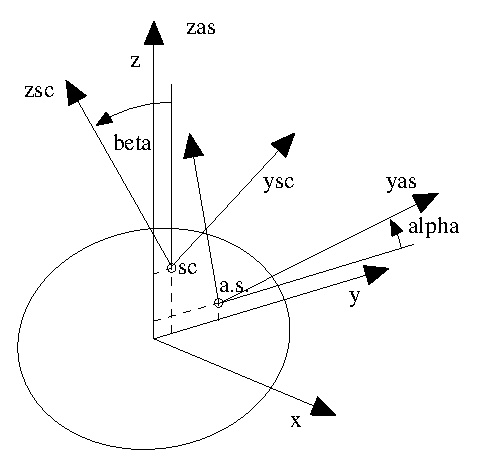
\includegraphics[width=.7\textwidth]{beamsect}
\caption{Beam section}
\label{fig:EL:BEAM:SECTION}
\end{figure}






\subsubsection{Generic Anisotropic Beam Section}
When a generic anisotropic beam section is considered,
the partitioning of axial and shear constitutive properties
of Figure~\ref{fig:EL:BEAM:GROUPS} is no longer possible.
The axial and shear straining can be completely and arbitrarily coupled,
resulting in a full constitutive matrix of the beam section,
\begin{align}
	\cubr{\cvvect{
		\T{f} \\
		\T{m}
	}}^\dagger
	&=
	\sqbr{\matr{cc}{
		\TT{K}_{\T{f}\T{\nu}} & \TT{K}_{\T{f}\T{\kappa}} \\
		\TT{K}_{\T{m}\T{\nu}} & \TT{K}_{\T{m}\T{\kappa}}
	}}^\dagger
	\cubr{\cvvect{
		\T{\nu} \\
		\T{\kappa}
	}}^\dagger ,
\end{align}
where $\T{f}$ and $\T{m}$ are the internal force and moment vectors,
while $\T{\nu}$ and $\T{\kappa}$ are the linear and angular strains.
Usually, $\TT{K}_{\T{m}\T{\nu}}\equiv\TT{K}_{\T{f}\T{\kappa}}^T$,
while $\TT{K}_{\T{f}\T{\nu}}$ and $\TT{K}_{\T{m}\T{\kappa}}$ are symmetric.


The reference point or the reference orientation of the constitutive
matrix can be changed by a sequence of transformations consisting
in a rotation and an offset.

The internal force and moment, after a rotation defined by the rotation
matrix $\TT{R}$, become
\begin{align}
	\cubr{\cvvect{
		\T{f} \\
		\T{m}
	}}^*
	&= \sqbr{\matr{cc}{
		\TT{R} & \TT{0} \\
		\TT{0} & \TT{R}
	}}
	\cubr{\cvvect{
		\T{f} \\
		\T{m}
	}}^\dagger
	.
\end{align}
Similarly, the strains become
\begin{align}
	\cubr{\cvvect{
		\T{\nu} \\
		\T{\kappa}
	}}^*
	&= \sqbr{\matr{cc}{
		\TT{R} & \TT{0} \\
		\TT{0} & \TT{R}
	}}^{-T}
	\cubr{\cvvect{
		\T{\nu} \\
		\T{\kappa}
	}}^\dagger
	\nonumber \\
	&= \sqbr{\matr{cc}{
		\TT{R} & \TT{0} \\
		\TT{0} & \TT{R}
	}}
	\cubr{\cvvect{
		\T{\nu} \\
		\T{\kappa}
	}}^\dagger
	.
\end{align}
As a consequence, the re-oriented constitutive relationship is
\begin{align}
	\cubr{\cvvect{
		\T{f} \\
		\T{m}
	}}^*
	&=
	\sqbr{\matr{cc}{
		\TT{R} & \TT{0} \\
		\TT{0} & \TT{R}
	}}
	\sqbr{\matr{cc}{
		\TT{K}_{\T{f}\T{\nu}} & \TT{K}_{\T{f}\T{\kappa}} \\
		\TT{K}_{\T{m}\T{\nu}} & \TT{K}_{\T{m}\T{\kappa}}
	}}^\dagger
	\sqbr{\matr{cc}{
		\TT{R} & \TT{0} \\
		\TT{0} & \TT{R}
	}}^T
	\cubr{\cvvect{
		\T{\nu} \\
		\T{\kappa}
	}}^*
	\nonumber \\
	&=
	\sqbr{\matr{cc}{
		\TT{R} \TT{K}_{\T{f}\T{\nu}}^\dagger \TT{R}^T
			& \TT{R} \TT{K}_{\T{f}\T{\kappa}}^\dagger \TT{R}^T \\
		\TT{R} \TT{K}_{\T{m}\T{\nu}}^\dagger \TT{R}^T
			& \TT{R} \TT{K}_{\T{m}\T{\kappa}}^\dagger \TT{R}^T
	}}
	\cubr{\cvvect{
		\T{\nu} \\
		\T{\kappa}
	}}^*
	\nonumber \\
	&=
	\sqbr{\matr{cc}{
		\TT{K}_{\T{f}\T{\nu}} & \TT{K}_{\T{f}\T{\kappa}} \\
		\TT{K}_{\T{m}\T{\nu}} & \TT{K}_{\T{m}\T{\kappa}}
	}}^*
	\cubr{\cvvect{
		\T{\nu} \\
		\T{\kappa}
	}}^*
	.
\end{align}

The internal moment, after considering an offset $\T{o}=\sqbr{0, y, z}^T$
of the reference point of the constitutive properties, becomes
$\T{m}=\T{m}^* + \T{o}\times\T{f}^*$.
The internal force and moment then becomes
\begin{align}
	\cubr{\cvvect{
		\T{f} \\
		\T{m}
	}}
	&= \sqbr{\matr{cc}{
		\TT{I} & \TT{0} \\
		\T{o}\times{} & \TT{I}
	}}
	\cubr{\cvvect{
		\T{f} \\
		\T{m}
	}}^*
	\label{eq:EL:BEAM:ANISOTROPIC-T}
	.
\end{align}
Similarly, the linear and angular strain vectors become
\begin{align}
	\cubr{\cvvect{
		\T{\nu} \\
		\T{\kappa}
	}}
	&= \sqbr{\matr{cc}{
		\TT{I} & \TT{0} \\
		\T{o}\times{} & \TT{I}
	}}^{-T}
	\cubr{\cvvect{
		\T{\nu} \\
		\T{\kappa}
	}}^*
	.
\end{align}
As a consequence, the offset constitutive relationship becomes
\begin{align}
	\cubr{\cvvect{
		\T{f} \\
		\T{m}
	}}
	&=
	\sqbr{\matr{cc}{
		\TT{I} & \TT{0} \\
		\T{o}\times{} & \TT{I}
	}}
	\sqbr{\matr{cc}{
		\TT{K}_{\T{f}\T{\nu}} & \TT{K}_{\T{f}\T{\kappa}} \\
		\TT{K}_{\T{m}\T{\nu}} & \TT{K}_{\T{m}\T{\kappa}}
	}}^*
	\sqbr{\matr{cc}{
		\TT{I} & \T{o}\times{}^T \\
		\TT{0} & \TT{I}
	}}
	\cubr{\cvvect{
		\T{\nu} \\
		\T{\kappa}
	}}
	\nonumber \\
	&=
	\sqbr{\matr{cc}{
		\TT{K}_{\T{f}\T{\nu}}^*
		& \TT{K}_{\T{f}\T{\nu}}^* \T{o}\times{}^T
			+ \TT{K}_{\T{f}\T{\kappa}}^* \\
		\T{o}\times\TT{K}_{\T{f}\T{\nu}}^*
			+ \TT{K}_{\T{m}\T{\nu}}^*
		& \T{o}\times\TT{K}_{\T{f}\T{\nu}}^* \T{o}\times{}^T
			+ \TT{K}_{\T{m}\T{\nu}}^* \T{o}\times{}^T
			+ \T{o}\times\TT{K}_{\T{f}\T{\kappa}}^*
			+ \TT{K}_{\T{m}\T{\kappa}}^*
	}}
	\cubr{\cvvect{
		\T{\nu} \\
		\T{\kappa}
	}}
	\nonumber \\
	&=
	\sqbr{\matr{cc}{
		\TT{K}_{\T{f}\T{\nu}} & \TT{K}_{\T{f}\T{\kappa}} \\
		\TT{K}_{\T{m}\T{\nu}} & \TT{K}_{\T{m}\T{\kappa}}
	}}
	\cubr{\cvvect{
		\T{\nu} \\
		\T{\kappa}
	}}^*
	.
\end{align}

It might be tempting to find what offset and rotation allows
to decouple the force and moment constitutive properties.
This can be sought by defining a generic transformation
\begin{align}
	\cubr{\cvvect{
		\T{f} \\
		\T{m}
	}}
	&= \sqbr{\matr{cc}{
		\TT{I} & \TT{0} \\
		\TT{T} & \TT{I}
	}}
	\cubr{\cvvect{
		\T{f} \\
		\T{m}
	}}^\dagger
	,
\end{align}
such that
\begin{align}
	\cubr{\cvvect{
		\T{f} \\
		\T{m}
	}}
	&=
	\sqbr{\matr{cc}{
		\TT{I} & \TT{0} \\
		\TT{T} & \TT{I}
	}}
	\sqbr{\matr{cc}{
		\TT{K}_{\T{f}\T{\nu}} & \TT{K}_{\T{f}\T{\kappa}} \\
		\TT{K}_{\T{m}\T{\nu}} & \TT{K}_{\T{m}\T{\kappa}}
	}}^\dagger
	\sqbr{\matr{cc}{
		\TT{I} & \TT{T}^T \\
		\TT{0} & \TT{I}
	}}
	\cubr{\cvvect{
		\T{\nu} \\
		\T{\kappa}
	}}
	\nonumber \\
	&=
	\sqbr{\matr{cc}{
		\TT{K}_{\T{f}\T{\nu}}^\dagger
		& \TT{K}_{\T{f}\T{\nu}}^\dagger \TT{T}^T
			+ \TT{K}_{\T{f}\T{\kappa}}^\dagger \\
		\TT{T}\TT{K}_{\T{f}\T{\nu}}^\dagger
			+ \TT{K}_{\T{m}\T{\nu}}^\dagger
		& \TT{T}\TT{K}_{\T{f}\T{\nu}}^\dagger \TT{T}^T
			+ \TT{K}_{\T{m}\T{\nu}}^\dagger \TT{T}^T
			+ \TT{T}\TT{K}_{\T{f}\T{\kappa}}^\dagger
			+ \TT{K}_{\T{m}\T{\kappa}}^\dagger
	}}
	\cubr{\cvvect{
		\T{\nu} \\
		\T{\kappa}
	}}
	.
\end{align}
The expected decoupling results from
\begin{align}
	\TT{T}
	&= 
	- \TT{K}_{\T{m}\T{\nu}}^\dagger
		\plbr{\TT{K}_{\T{f}\T{\nu}}^\dagger}^{-1}
	.
\end{align}
However, the resulting transformation $\TT{T}$ is not guaranteed
to have the skew-symmetric structure of $\T{o}\times{}$,
thus the decoupling may not be reducible to an offset.

The reverse transformation is relatively straightforward, after noticing
that, according to Eq.~(\ref{eq:EL:BEAM:ANISOTROPIC-T}), 
\begin{align}
	\cubr{\cvvect{
		\T{f} \\
		\T{m}
	}}^*
	&= \sqbr{\matr{cc}{
		\TT{I} & \TT{0} \\
		\T{o}\times{} & \TT{I}
	}}^{-1}
	\cubr{\cvvect{
		\T{f} \\
		\T{m}
	}}
	\nonumber \\
	&= \sqbr{\matr{cc}{
		\TT{I} & \TT{0} \\
		-\T{o}\times{} & \TT{I}
	}}
	\cubr{\cvvect{
		\T{f} \\
		\T{m}
	}}
	.
\end{align}
So, as expected, it is sufficient to revert the sign of the offset
to revert the transformation.
The signs of the constitutive relationship change accordingly.


\subsubsection{Locking Correction for Two-Node Beam}
The three-node finite volume element has been implemented first, 
and uses conventional polynomial parabolic interpolation 
of the nodal displacements and orientations;
the two-node finite volume element has been introduced later.
This latter element presents some shear-locking, which, for linear elastic
constitutive laws, may be overcome by correcting the section stiffness matrix
in a relatively straightforward form:
\begin{equation}\label{eq:2-NODE-BEAM-STIFFNESS}
	\hat{\T{K}} = \plbr{\T{F} + \frac{L^2}{12}\T{T} \T{F} \T{T}^T}^{-1} ,
\end{equation}
where $\T{F}=\T{K}^{-1}$ is the compliance matrix of the section, 
$L$ is the length of the beam, i.e.\ the distance between
the two reference points obtained by adding the optional offset 
to the nodes, and
\begin{displaymath}
	\T{T} \ = \ \sqbr{\matr{cc}{
		\T{0} & \T{e}_x \times{} \\
		\T{0} & \T{0}
	}}
\end{displaymath}
is the ``arm'' matrix that appears in the differential equilibrium equation
\begin{displaymath}
	\T{\vartheta}_{/x} - \T{T}^T\T{\vartheta} + \T{\phi} = 0
	,
\end{displaymath}
where $\T{\vartheta}=\sqbr{\T{f}^T \T{m}^T}^T$ are the internal forces
and moments, while $\T{\phi}$ are the external forces and moments
per unit span.

There are no provisions to automatically apply the correction 
when defining the constitutive law of the section.
The two-node beam has been re-implemented using a helicoidal interpolation
of the nodal positions and orientations, to improve its capability
to undergo large displacements and relative rotations.
It is activated by using the keyword \kw{hbeam2} instead of \kw{beam2}.
However, to reduce the shear-locking effect, the stiffness properties 
still need to be manually corrected according
to Equation~(\ref{eq:2-NODE-BEAM-STIFFNESS}).
The \kw{hbeam2} element is \emph{experimental}, and should be used
only for development purposes.


\subsection{Three-node beam element}
\label{sec:EL:BEAM:BEAM3}
The three-node beam element is described in detail in \cite{FV-AIAA}.
Each of the three points the beam element connects is referred
to a structural node but can have an arbitrary offset
to allow high generality in locating the structural reference line
of the beam.
Figure~\ref{fig:EL:BEAM:beam3} illustrates the geometry
of the three-node beam element.

\begin{figure}
\centering
\psfrag{1}{1}
\psfrag{2}{2}
\psfrag{3}{3}
\psfrag{n1}{node 1}
\psfrag{n2}{node 2}
\psfrag{n3}{node 3}
\psfrag{pI}{point I}
\psfrag{pII}{point II}
\psfrag{o1}{$\T{o}_1$}
\psfrag{o2}{$\T{o}_2$}
\psfrag{o3}{$\T{o}_3$}
\psfrag{RI}{$\TT{R}_I$}
\psfrag{RII}{$\TT{R}_{II}$}
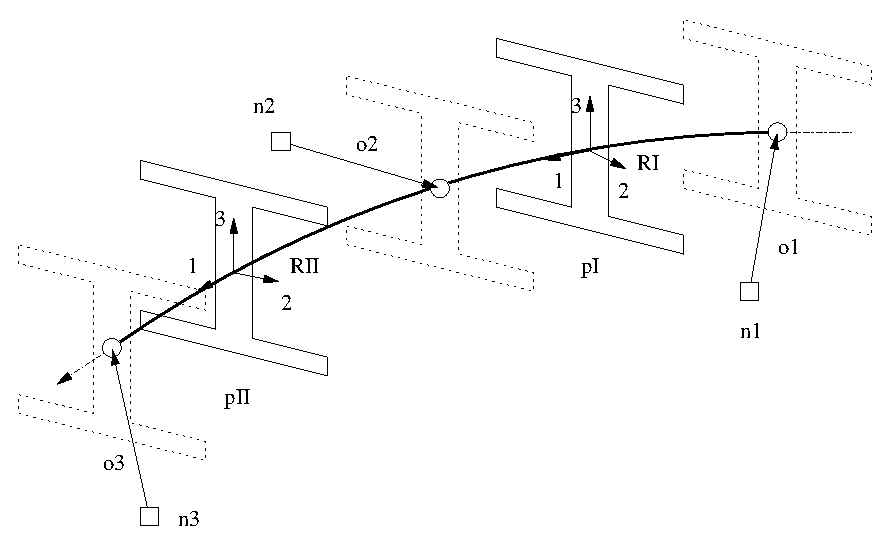
\includegraphics[width=.7\textwidth]{beam3}
\caption{Geometry of the three-node beam element.}
\label{fig:EL:BEAM:beam3}
\end{figure}

The finite volume formulation presented in \cite{FV-AIAA} is used.
As a consequence, the internal forces and moments are evaluated 
at two points that are at about midpoint between nodes 1 and 2, 
and nodes 2 and 3 (at $ \xi=-1/\sqrt{3}\cong -0.57735 $
and $\xi=1/\sqrt{3} \cong 0.57735$ of a non-dimensional abscissa $\xi$
running from $\xi=-1$ at node 1 to $\xi=1$ at node 3).

So the constitutive properties must be supplied in these points, as well as
the orientation matrices $\TT{R}_I$ and $\TT{R}_{II}$,
that express the orientation of the reference system
the constitutive properties are expressed in with respect to the global frame
(the axial force is conventionally defined in direction 1).
Any of the supported 6D constitutive laws can be supplied to define the
constitutive properties of each beam section.

The traditional input format is
%\begin{verbatim}
\begin{Verbatim}[commandchars=\\\{\}]
    \bnt{elem_type} ::= \kw{beam3}

    \bnt{normal_arglist} ::=
        \bnt{node_1_label} , (\hty{Vec3}) \bnt{relative_offset_1} ,
        \bnt{node_2_label} , (\hty{Vec3}) \bnt{relative_offset_2} ,
        \bnt{node_3_label} , (\hty{Vec3}) \bnt{relative_offset_3} ,
        (\hty{OrientationMatrix}) \bnt{orientation_matrix_section_I} ,
        (\htybkw{ConstitutiveLaw}{6D}) \bnt{constitutive_law_section_I} ,
        \{ \kw{same} | (\hty{OrientationMatrix}) \bnt{orientation_matrix_section_II} \} ,
        \{ \kw{same} | (\htybkw{ConstitutiveLaw}{6D}) \bnt{constitutive_law_section_II} \}
        [ , \bnt{custom_output} ]
\end{Verbatim}
%\end{verbatim}

The \nt{relative\_offset\_}\bnt{i}, with \nt{i}=1,2,3, are the vectors
$\T{o}_i$, with $i$=1,2,3, of Figure~\ref{fig:EL:BEAM:beam3}.

The orientation matrices \nt{orientation\_matrix\_section\_}\bnt{j},
with \nt{j}=I,II, are the section orientation matrices
$\TT{R}_j$, with $j$=$I$,$II$, of Figure~\ref{fig:EL:BEAM:beam3}.
They represent the (absolute) orientation in which the respective
constitutive properties are expressed.

The first keyword \kw{same}, alternative to the 
\nt{orientation\_matrix\_section\_II}, means that the same orientation
defined for the first point will be used for the second point.

The second keyword \kw{same}, alternative to the
\nt{constitutive\_law\_section\_II}, means that the same constitutive law
defined for the first point will be used for the second point.

If any of the constitutive laws is either viscous or viscoelastic,
the viscoelastic variant of the beam element is used.
Otherwise, the elastic variant is used.

A more complete input format is
%\begin{verbatim}
\begin{Verbatim}[commandchars=\\\{\}]
    \bnt{elem_type} ::= \kw{beam3}

    \bnt{normal_arglist} ::=
        \bnt{node_1_label} ,
            [ \kw{position} , ] (\hty{Vec3}) \bnt{relative_offset_1} ,
            [ \kw{orientation} , (\hty{OrientationMatrix}) \bnt{relative_orientation_1} , ]
        \bnt{node_2_label} ,
            [ \kw{position} , ] (\hty{Vec3}) \bnt{relative_offset_2} ,
            [ \kw{orientation} , (\hty{OrientationMatrix}) \bnt{relative_orientation_2} , ]
        \bnt{node_3_label} ,
            [ \kw{position} , ] (\hty{Vec3}) \bnt{relative_offset_3} ,
            [ \kw{orientation} , (\hty{OrientationMatrix}) \bnt{relative_orientation_3} , ]
        \{ (\hty{OrientationMatrix}) \bnt{orientation_matrix_section_I}
            | \kw{from nodes} \} ,
        (\htybkw{ConstitutiveLaw}{6D}) \bnt{constitutive_law_section_I} ,
        \{ \kw{same}
            | (\hty{OrientationMatrix}) \bnt{orientation_matrix_section_II}
            | \kw{from nodes} \} ,
        \{ \kw{same}
            | (\htybkw{ConstitutiveLaw}{6D}) \bnt{constitutive_law_section_II} \}
        [ , \bnt{custom_output} ]
\end{Verbatim}
%\end{verbatim}
This format is a superset of the traditional one, which is extended
by adding the possibility to set, for each node, the relative orientation
\nt{relative\_orientation\_}\bnt{i}, with \nt{i}=1,2,3,
with respect to the node itself.
Such orientation can be subsequently used to interpolate the orientation matrices
at the evaluation points, by providing the keyword \kw{from nodes}
instead of the orientation matrix.
If the keyword \kw{same} is used for the second evaluation point,
the same method is used to compute the orientation matrix.

The \nt{custom\_output} optional data consists in
%\begin{verbatim}
\begin{Verbatim}[commandchars=\\\{\}]
    \bnt{custom_output} ::= \kw{custom output} , \bnt{custom_output_flag} [ , ... ]
\end{Verbatim}
%\end{verbatim}
The values of \nt{custom\_output\_flag}
are defined in Section~\ref{sec:CONTROLDATA:DEFAULTBEAMOUTPUT}.

Flags add up to form the custom output request.
Flags may not be repeated.
Strain rates are only available from viscoelastic beams.
By default, only forces are output, to preserve compatibility
with the original output format.
The custom output is only available in NetCDF format;
see Section~\ref{sec:NetCDF:Elem:Beam}.

As an example, a simple beam element, with diagonal section stiffness 
matrix is presented:
\begin{verbatim}
    set: integer beam_label = 1000;
    set: integer beam_node1 = 2001;
    set: integer beam_node2 = 2002;
    set: integer beam_node3 = 2003;
    set: real EA = 1e6;   # N
    set: real GAy = .6e6; # N
    set: real GAz = .6e6; # N
    set: real GJ = 1.e3;  # Nm^2
    set: real EJy = 2.e3; # Nm^2
    set: real EJz = 1.e4; # Nm^2
    beam3: beam_label,
        beam_node1, reference, node, null,
        beam_node2, reference, node, null,
        beam_node3, reference, node, null,
        eye,
        linear elastic generic, diag,
            EA, GAy, GAz, GJ, EJy, EJz,
        same,
        same;
\end{verbatim}

A not-so-simple beam section, where the center of axial strain 
and the shear center are not coincident, is illustrated below.
The node offset is used to align the reference line 
with the shear center, and the axial strain center offset 
is used in the constitutive matrix:
\begin{verbatim}
    set: integer beam_label = 1000;
    set: integer beam_node1 = 2001;
    set: integer beam_node2 = 2002;
    set: integer beam_node3 = 2003;
    set: real EA = 1e6;    # N
    set: real GAy = .6e6;  # N
    set: real GAz = .6e6;  # N
    set: real GJ = 1.e3;   # Nm^2
    set: real EJy = 2.e3;  # Nm^2
    set: real EJz = 1.e4;  # Nm^2
    set: real yas = 2.e-2; # m
    set: real zas = 1.e-2; # m
    set: real ysc = 4.e-2; # m
    set: real zsc = 2.e-2; # m
    set: real y = yas-ysc; # compute the axial strain center
    set: real z = zas-zsc; # wrt/ the shear center
    beam3: beam_label,
        beam_node1, reference, node, 0.,ysc,zsc,
        beam_node2, reference, node, 0.,ysc,zsc,
        beam_node3, reference, node, 0.,ysc,zsc,
        eye,
        linear elastic generic, sym,
            EA, 0.,  0.,  0., z*EA,       -y*EA,
                GAy, 0.,  0., 0.,          0.,
                     GAz, 0., 0.,          0.,
                          GJ, 0.,          0.,
                              EJy+z^2*EA, -z*y*EA,
                                           EJz+y^2*EA,
        same,
        same;
\end{verbatim}


A piezoelectric actuator beam element is available; an arbitrary
linear piezoelectric actuation matrix is required, together with the labels
of the abstract nodes that represent the input signal tensions, as follows:
%\begin{verbatim}
\begin{Verbatim}[commandchars=\\\{\}]
    \bnt{normal_arglist} ::=
        \bnt{node_1_label} , (\hty{Vec3}) \bnt{relative_offset_1} ,
        \bnt{node_2_label} , (\hty{Vec3}) \bnt{relative_offset_2} ,
        \bnt{node_3_label} , (\hty{Vec3}) \bnt{relative_offset_3} ,
        (\hty{OrientationMatrix}) \bnt{orientation_matrix_section_I} ,
        (\htybkw{ConstitutiveLaw}{6D}) \bnt{constitutive_law_section_I} ,
        \{ \kw{same} | (\hty{OrientationMatrix}) \bnt{orientation_matrix_section_II} \} ,
        \{ \kw{same} | (\htybkw{ConstitutiveLaw}{6D}) \bnt{constitutive_law_section_II} \} ,
        \kw{piezoelectric actuator} , 
            \bnt{electrodes_number} ,
            \bnt{abstract_node_label_list} ,
            (\hty{Mat6xN}) \bnt{piezoelectric_matrix_I} ,
            \{ \kw{same} | (\hty{Mat6xN}) \bnt{piezoelectric_matrix_II} \}
        [ , \bnt{custom_output} ]
\end{Verbatim}
%\end{verbatim}
where the \nt{abstract\_node\_label\_list} is the list of the labels of the
abstract nodes that represent the electrodes.

A fully coupled piezoelectric beam element is available as well; an arbitrary
linear piezoelectric actuation matrix is required, together with the labels
of the abstract nodes that represent the input signal tensions, as follows:
%\begin{verbatim}
\begin{Verbatim}[commandchars=\\\{\}]
    \bnt{normal_arglist} ::=
        \bnt{node_1_label} , (\hty{Vec3}) \bnt{relative_offset_1} ,
        \bnt{node_2_label} , (\hty{Vec3}) \bnt{relative_offset_2} ,
        \bnt{node_3_label} , (\hty{Vec3}) \bnt{relative_offset_3} ,
        (\hty{OrientationMatrix}) \bnt{orientation_matrix_section_I} ,
        (\htybkw{ConstitutiveLaw}{6D}) \bnt{constitutive_law_section_I} ,
        \{ \kw{same} | (\hty{OrientationMatrix}) \bnt{orientation_matrix_section_II} \} ,
        \{ \kw{same} | (\htybkw{ConstitutiveLaw}{6D}) \bnt{constitutive_law_section_II} \} ,
        \kw{piezoelectric beam} , 
            \bnt{electrodes_number} ,
            \bnt{abstract_node_label_list} ,
            (\hty{Mat6xN}) \bnt{piezoelectric_matrix_I} ,
            (\hty{MatNx6}) \bnt{piezoelectric_charges_def_I} ,
            (\hty{MatNxN}) \bnt{piezoelectric_charges_potential_I} ,
            \{ 
                \kw{same}
               |
                (\hty{Mat6xN}) \bnt{piezoelectric_matrix_II} 
                (\hty{MatNx6}) \bnt{piezoelectric_charges_def_II} ,
                (\hty{MatNxN}) \bnt{piezoelectric_charges_potential_II}
            \}
        [ , \bnt{custom_output} ]
\end{Verbatim}
%\end{verbatim}
where the \nt{abstract\_node\_label\_list} is the list of the labels of the
abstract nodes that represent the electrodes, \nt{piezoelectric\_charges\_def} give
to compute the charge per unit of length as a function of the beam generalized
deformation measures, and \nt{piezoelectric\_charges\_potential} the charge per unit of length 
as a function of the electrodes potential.


\paragraph{Private Data}
\label{sec:EL:BEAM:PRIVATE}
The following data are available:
\begin{enumerate}
\item \kw{"ex"} axial strain
\item \kw{"ey"} shear strain (local axis 2)
\item \kw{"ez"} shear strain (local axis 3)
\item \kw{"kx"} curvature about local axis 1 (torsional)
\item \kw{"ky"} curvature about local axis 2 (bending)
\item \kw{"kz"} curvature about local axis 3 (bending)
\item \kw{"Fx"} axial force
\item \kw{"Fy"} shear force (direction 2)
\item \kw{"Fz"} shear force (direction 3)
\item \kw{"Mx"} moment about local axis 1 (torsional)
\item \kw{"My"} moment about local axis 2 (bending)
\item \kw{"Mz"} moment about local axis 3 (bending)
\item \kw{"Xx"} absolute position component 1
\item \kw{"Xy"} absolute position component 2
\item \kw{"Xz"} absolute position component 3
\item \kw{"Phix"} absolute orientation vector component 1
\item \kw{"Phiy"} absolute orientation vector component 2
\item \kw{"Phiz"} absolute orientation vector component 3
\item \kw{"Omegax"} absolute angular velocity component 1
\item \kw{"Omegay"} absolute angular velocity component 2
\item \kw{"Omegaz"} absolute angular velocity component 3
\item \kw{"ePx"} axial strain rate
\item \kw{"ePy"} shear strain rate (local axis 2)
\item \kw{"ePz"} shear strain rate (local axis 3)
\item \kw{"kPx"} curvature rate about local axis 1 (torsional)
\item \kw{"kPy"} curvature rate about local axis 2 (bending)
\item \kw{"kPz"} curvature rate about local axis 3 (bending)
\end{enumerate}
Each string is prefixed by \kw{"pI."} or \kw{"pII."}
to specify data related to either the first or the second point:
\begin{verbatim}
    "pI.Fx"     # axial force at point I
    "pII.kz"    # bending curvature about local axis 3 at point II
\end{verbatim}
Private data related to point I are numbered from 1 to 27;
private data related to point II are numbered from 28 to 54.



\subsubsection{Inertia Properties}
So-called ``consistent inertia'' is not implemented for beam elements; one needs to use \kw{body} (rigid-body) elements 
(Section~\ref{sec:EL:BODY}) instead.
Their suggested usage is detailed here.

In principle, from the inertial point of view, the beam should be split in ``chunks'' as discussed earlier.
Distributed inertia loads are associated with the motion of each chunk.
For moderate straining, one can safely assume that the chunks remain rigid with respect to inertia loads computation.

For the sake of simplicity, it is assumed that the beam is straight, with uniform inertia properties,
where the $x$ axis is the beam axis, and $y$ and $z$ are principal inertia axes of the section.
Moreover, it is assumed that the nodes are equally spaced (i.e.\ the mid-node is at midspan).

Consider the mass per unit span $m$, the inertia moment per unit span about the beam's axis, $i_{xx}$,
and those about the two remaining axes, $i_{yy}$, $i_{zz}$, with $i_{xx} = i_{yy} + i_{zz}$.
The length of the beam element is $\ell$.

According to the theory, the beam is cut at two stations, set at $\pm \ell/(2 \sqrt{3})$ from the mid-node.
As a consequence, the length of the middle chunk is $\ell_{\text{mid}} = \ell/\sqrt{3}$, whereas that of the end chunks is
$\ell_{\text{end}} = \ell (1 - 1/\sqrt{3})/2$.

The corresponding bodies are
\begin{verbatim}
# body associated with first end node
body: 1,
    1, # label of first end node
    m*ell_end, # mass associated with first end node
    reference, node, ell_end/2, 0., 0., # the center of mass of this chunk
                                        # is offset along the beam axis
    diag,
        i_xx*ell_end,
        i_yy*ell_end + m*ell_end^3/12, # i_yy may often be neglected
        i_zz*ell_end + m*ell_end^3/12; # i_zz may often be neglected

# body associated with mid-node
body: 2,
    2, # label of mid-node
    m*ell_mid, # mass associated with mid-node
    reference, node, null, # the center of mass of this chunk is at the node
    diag,
        i_xx*ell_mid,
        i_yy*ell_mid + m*ell_mid^3/12,
        i_zz*ell_mid + m*ell_mid^3/12;

# body associated with last end node
body: 3,
    3, # label of last end node
    m*ell_end,
    reference, node, -ell_end/2, 0., 0.,
    diag,
        i_xx*ell_end,
        i_yy*ell_end + m*ell_end^3/12,
        i_zz*ell_end + m*ell_end^3/12;
\end{verbatim}
Often, $i_{yy}$ and $i_{zz}$ can be neglected, significantly when the beam element is slender enough
(i.e.\ when $\ell \sqrt{m A/i_{yy}} \approx \ell \sqrt{m A/i_{zz}} \ll 1$).

Moreover, the chunks do not necessarily need to be cut exactly at $\pm \ell / (2 \sqrt{3})$;
setting $\ell_{\text{mid}} = \ell/2$ and $\ell_{\text{end}} = \ell/4$ gives good results.

When assembling strings of beam elements, one would need to connect two \kw{body} elements to each end node,
each of them accounting from the inertial contribution of the two adjacent beam elements.
Alternatively, a single \kw{body} can be used, which accounts for the contribution of the two elements.
If the two adjacent beam elements are identical (i.e.\ same inertia properties, same length $\ell$),
an end body would look like
\begin{verbatim}
body: 3,
    3, # label of last end node
    m*(2*ell_end),
    reference, node, null,
    diag,
        i_xx*(2*ell_end),
        i_yy*(2*ell_end) + m*(2*ell_end)^3/12,
        i_zz*(2*ell_end) + m*(2*ell_end)^3/12;
\end{verbatim}
If the two adjacent beam elements differ, one can use the \kw{condense} option
to collect the inertia contributions from each beam element and let the solver
do the merge.
See Section~\ref{sec:EL:BODY} for more details.

If the beam element is significantly curved, one needs to evaluate the correct position of the center of mass,
and correct the inertia tensor accordingly.

If axes $y$, $z$ are not principal inertia axes, one needs to take into account the cross-coupling terms in the inertia tensor.





\subsection{Two-node beam element}
\label{sec:EL:BEAM:BEAM2}
Similar considerations apply to the two-node beam.
Its geometry is illustrated in Figure~\ref{fig:EL:BEAM:beam2}.

\begin{figure}
\centering
\psfrag{1}{1}
\psfrag{2}{2}
\psfrag{3}{3}
\psfrag{n1}{node 1}
\psfrag{n2}{node 2}
\psfrag{pI}{point I}
\psfrag{o1}{$\T{o}_1$}
\psfrag{o2}{$\T{o}_2$}
\psfrag{RI}{$\TT{R}_I$}
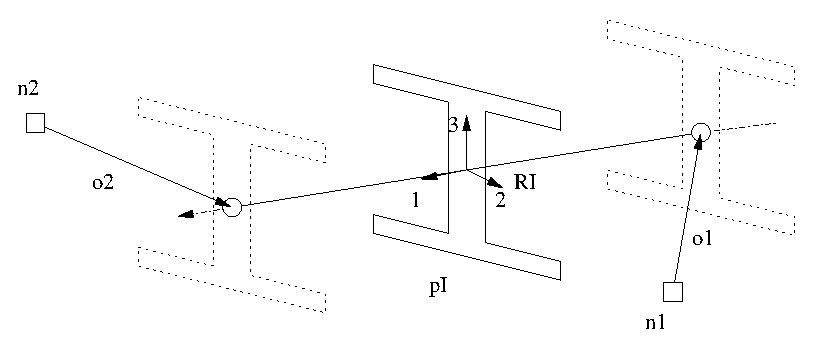
\includegraphics[width=.7\textwidth]{beam2}
\caption{Geometry of the two-node beam element.}
\label{fig:EL:BEAM:beam2}
\end{figure}

The syntax is
%\begin{verbatim}
\begin{Verbatim}[commandchars=\\\{\}]
    \bnt{elem_type} ::= \kw{beam2}

    \bnt{normal_arglist} ::=
        \bnt{node_1_label} , (\hty{Vec3}) \bnt{relative_offset_1} ,
        \bnt{node_2_label} , (\hty{Vec3}) \bnt{relative_offset_2} ,
        (\hty{OrientationMatrix}) \bnt{orientation_matrix_section_I} ,
        (\htybkw{ConstitutiveLaw}{6D}) \bnt{constitutive_law_section_I}
        [ , \kw{piezoelectric actuator} , 
            \bnt{electrodes_number} ,
            \bnt{abstract_node_label_list} ,
            (\hty{Mat6xN}) \bnt{piezoelectric_matrix_I} ]
        [ , \bnt{custom_output} ]
\end{Verbatim}
%\end{verbatim}

A more complete form is
%\begin{verbatim}
\begin{Verbatim}[commandchars=\\\{\}]
    \bnt{elem_type} ::= \kw{beam2}

    \bnt{normal_arglist} ::=
        \bnt{node_1_label} ,
            [ \kw{position} , ] (\hty{Vec3}) \bnt{relative_offset_1} ,
            [ \kw{orientation} , (\hty{OrientationMatrix}) \bnt{relative_orientation_1} , ]
        \bnt{node_2_label} ,
            [ \kw{position} , ] (\hty{Vec3}) \bnt{relative_offset_2} ,
            [ \kw{orientation} , (\hty{OrientationMatrix}) \bnt{relative_orientation_2} , ]
        \{ (\hty{OrientationMatrix}) \bnt{orientation_matrix_section_I}
            | \kw{from nodes} \} ,
        (\htybkw{ConstitutiveLaw}{6D}) \bnt{constitutive_law_section_I}
        [ , \kw{piezoelectric actuator} , 
            \bnt{electrodes_number} ,
            \bnt{abstract_node_label_list} ,
            (\hty{Mat6xN}) \bnt{piezoelectric_matrix_I} ]
        [ , \bnt{custom_output} ]
\end{Verbatim}
%\end{verbatim}

\paragraph{Private Data.}
The same private data indicated for the \kw{beam3} element is available
(see Section~\ref{sec:EL:BEAM:PRIVATE}).
No prefix must be specified (\kw{"pI."} is implicit).


\paragraph{Example.} \
As an example, a simple beam element, with diagonal section stiffness 
matrix is presented:
\begin{verbatim}
    set: integer beam_label = 1000;
    set: integer beam_node1 = 2001;
    set: integer beam_node2 = 2002;
    set: real L = .4;     # m
    set: real EA = 1e6;   # N
    set: real GAy = .6e6; # N
    set: real GAz = .6e6; # N
    set: real GJ = 1.e3;  # Nm^2
    set: real EJy = 2.e3; # Nm^2
    set: real EJz = 1.e4; # Nm^2
    beam2: beam_label,
        beam_node1, reference, node, null,
        beam_node2, reference, node, null,
        eye,
        linear elastic generic, diag,
            EA, 1./(1./GAy+L^2/12./EJz), 1./(1./GAz+L^2/12./EJy),
            GJ, EJy, EJz;
\end{verbatim}
Note that the shear terms have been na\"{\i}vely inverted to eliminate
shear locking, according to Equation~(\ref{eq:2-NODE-BEAM-STIFFNESS}).


\subsubsection{Inertia Properties}
According to the theory, the beam is cut in half.
As a consequence, the length of each chunk is $\ell_{\text{end}} = \ell/2$.

With reference to the symbols defined for the three-node beam element, the corresponding bodies are
\begin{verbatim}
# body associated with first end node
body: 1,
    1, # label of first end node
    m*ell_end, # mass associated with first end node
    reference, node, ell_end/2, 0., 0., # the center of mass of this chunk
                                        # is offset along the beam axis
    diag,
        i_xx*ell_end,
        i_yy*ell_end + m*ell_end^3/12, # i_yy may often be neglected
        i_zz*ell_end + m*ell_end^3/12; # i_zz may often be neglected

# body associated with last end node
body: 2,
    2, # label of last end node
    m*ell_end,
    reference, node, -ell_end/2, 0., 0.,
    diag,
        i_xx*ell_end,
        i_yy*ell_end + m*ell_end^3/12,
        i_zz*ell_end + m*ell_end^3/12;
\end{verbatim}
Similar considerations to those made for the three-node beam element apply also in this case.



\subsection{Output}
The output related to beam elements is contained in a file with extension 
\texttt{.act}; for each time step, the output is written
for those element it was requested.
The internal forces and moments are computed from the interpolated strains
along the beam by means of the constitutive law, at the evaluation points. 
The format is:
\begin{itemize}
    \item column 1: the label of the beam;
    \item columns 2--4: the three components of the force
	at the first evaluation point, oriented according
	to the reference frame of that beam section;
    \item columns 5--7: the three components of the moment
	at the first evaluation point, oriented according
	to the reference frame of that beam section.
\end{itemize}

The three-node beam element generates six additional columns:
\begin{itemize}
    \item columns 8--10: the three components of the force
	at the second evaluation point, oriented according
	to the reference frame of that beam section;
    \item columns 11--13: the three components of the moment
	at the second evaluation point, oriented according
	to the reference frame of that beam section.
\end{itemize}

More detailed output is allowed when using NetCDF;
see Section~\ref{sec:NetCDF:Elem:Beam} for details.



\subsection{Notes}
Two-node beam elements should be used with care.



\section{Body}
\label{sec:EL:BODY}
The \kw{body} element describes a lumped rigid body when connected 
to a regular, 6 degree of freedom structural node, or a point mass
when connected to a rotationless, 3 degree of freedom structural node.
%\begin{verbatim}
\begin{Verbatim}[commandchars=\\\{\}]
    \bnt{elem_type} ::= \kw{body}

    \bnt{normal_arglist} ::= \bnt{node_label} ,
        \{ [ \kw{allow negative mass} , ] \bnt{one_body}
            | [ \kw{allow negative mass} , ] \bnt{one_pointmass}
            | \kw{variable mass} , \bnt{one_vm_body}
            | \kw{condense} , \bnt{num_masses} [ , \kw{allow negative mass} ] ,
	        \{ \bnt{one_body} | \bnt{one_pointmass} \} [ , ... ] \}

    \bnt{one_body} ::=
        (\ty{real}) \bnt{mass} , 
        (\hty{Vec3})   \bnt{relative_center_of_mass} ,
        (\hty{Mat3x3}) \bnt{inertia_matrix}
        [ , \kw{orientation} , (\hty{OrientationMatrix}) \bnt{orientation_matrix}]

    \bnt{one_pointmass} ::=
        (\ty{real}) \bnt{mass}      # when \bnt{node_label} is a \kw{displacement} node

    \bnt{one_vm_body} ::=
        (\hty{DriveCaller})            \bnt{mass} ,
        (\htybty{TplDriveCaller}{Vec3})   \bnt{relative_center_of_mass} ,
        (\htybty{TplDriveCaller}{Mat3x3}) \bnt{variable_mass_inertia_matrix} ,
        (\htybty{TplDriveCaller}{Mat3x3}) \bnt{variable_geometry_inertia_matrix}
\end{Verbatim}
%\end{verbatim}
If only one mass is defined, the first method should be used. Otherwise,
many masses can be referred to the same element by means of the keyword
\kw{condense}, followed by the number of expected masses \nt{num\_masses}.
The format of each sub-mass is the same as for the single mass input (actually, 
when \kw{condense} is not supplied, \nt{num\_masses} is assumed to be 1).
If \kw{allow negative mass} is specified, it will be possible to use
negative masses for the body. \textit{Warning}: the negative mass feature
is not officially supported and could cause unexpected behavior (for
example, gravity will still act as if the mass was positive).

The \nt{inertia\_matrix} is always referred to the center of mass of the
mass that is being added. It can be rotated locally by means of the extra
\nt{orientation\_matrix} supplied after the (optional) keyword 
\kw{orientation}.

Note: in many commercial finite element software, the off-diagonal elements 
of the inertia matrix are defined with a minus sign; for instance, 
NASTRAN's \texttt{CONM2} lumped inertia card expects the values as indicated
in Figure~\ref{fig:el:body:CONM2}.
%
\begin{figure}[b]
\centering
\begin{minipage}{120mm}
\begin{boxedverbatim}
$.......2.......3.......4.......5.......6.......7.......8.......
CONM2   EID     G       CID     M       X1      X2      X3
        I11     I21     I22     I31     I32     I33
\end{boxedverbatim}
\end{minipage}
\caption{NASTRAN \texttt{CONM2} card}
\label{fig:el:body:CONM2}
\end{figure}
%
However, the matrix is reconstructed as
\begin{displaymath}
	\mathrm{NASTRAN \ ::= } \ \sqbr{\matr{rrrrrr}{
		\texttt{M} & & & & & \\
		& \texttt{M} & & \multicolumn{3}{c}{\text{symmetric}} \\
		& & \texttt{M} & & & \\
		& & & \texttt{I11} & & \\
		& & & -\texttt{I21} & \texttt{I22} & \\
		& & & -\texttt{I31} & -\texttt{I32} & \texttt{I33}
	}}
\end{displaymath}
see for instance \emph{NASTRAN V70.5 Quick Reference Guide} for details.

\noindent
On the contrary, MBDyn directly reads the matrix 
that will be used in the computation, i.e.\ 
\textbf{without the minus signs in the off-diagonal terms},
as reported below:
\begin{displaymath}
	\mathrm{MBDyn \ ::= } \ \sqbr{\matr{ccc}{
		\texttt{i11} & \texttt{i12} & \texttt{i13} \\
		& \texttt{i22} & \texttt{i23} \\
		\multicolumn{2}{l}{\text{sym.}} & \texttt{i33}
	}}
\end{displaymath}
So:
\begin{eqnarray*}
	\texttt{i11} & = & \texttt{I11} \\
	\texttt{i22} & = & \texttt{I22} \\
	\texttt{i33} & = & \texttt{I33} \\
	\texttt{i12} & = & - \texttt{I21} \\
	\texttt{i13} & = & - \texttt{I31} \\
	\texttt{i23} & = & - \texttt{I32}
\end{eqnarray*}

The \kw{variable mass} variant requires the mass, \nt{mass},
the location of the center of mass with respect to the node
in the reference frame of the node, \nt{relative\_center\_of\_mass},
and the inertia matrix about the center of mass must be provided
in form of \emph{differentiable} drive callers of the specific dimension.
The inertia matrix is logically split in two contributions:
the first one, \nt{variable\_mass\_inertia\_matrix},
is related to the variation of mass;
the second one, \nt{variable\_geometry\_inertia\_matrix},
is related to the change of geometry at fixed instantaneous value
of the mass.
The instantaneous inertia matrix with respect to the node,
in the reference frame of the node, is computed as
\begin{align}
	\tilde{\TT{J}}_n
	&=
	\nt{variable\_mass\_inertia\_matrix}
	\noindent \\
	&\mbox{\hphantom{= }}
	+
	\nt{variable\_geometry\_inertia\_matrix}
	\noindent \\
	&\mbox{\hphantom{= }}
	+
	\nt{mass}
	\cdot
	\nt{relative\_center\_of\_mass} \times \nt{relative\_center\_of\_mass} \times{}^T
	.
\end{align}
See the technical manual for more details.

The inertia properties of the model can be logged and verified
by means of the \kw{inertia} keyword, as detailed
in Section~\ref{sec:EL:MISC:INERTIA}.

\paragraph{Private Data}
The following data are available:
\begin{enumerate}
\item \kw{"E"} kinetic energy
\item \kw{"V"} potential (i.e.\ gravitational) energy
\item \kw{"m"} mass
\end{enumerate}

\paragraph{Example.} \
\begin{verbatim}
    set: integer NODE_LABEL = 100;
    set: integer BODY_LABEL = 100;

    # single mass example
    body: BODY_LABEL, NODE_LABEL,
        8.,                            # mass
        reference, node, 0., 0., 0.,   # c.m. offset
        diag, 4.8, 4.8, .4;            # inertia tensor

    # three masses example (equivalent to the previous one)
    body: BODY_LABEL, NODE_LABEL,
        condense, 3,
        4.,                            # mass 1 (mid)
        reference, node, 0., 0., 0.,   # c.m. offset 1
        diag, .4, .4, .2,              # inertia tensor 1
        2.,                            # mass 2 (top)
        reference, node, 0., 0., 1.,   # c.m. offset 2
        diag, .2, .2, .1,              # inertia tensor 2
        2.,                            # mass 3 (bottom)
        reference, node, 0., 0., -1.,  # c.m. offset 3
        diag, .2, .2, .1;              # inertia tensor 3
\end{verbatim}



\section{Bulk Elements}
The \kw{bulk} element is intended as a sort of NASTRAN's \texttt{CELAS} card,
that can be used to apply a stiffness term on an arbitrary degree of freedom.
Extensions are planned to different kind of elements.
The syntax of the \kw{bulk} element is:
%\begin{verbatim}
\begin{Verbatim}[commandchars=\\\{\}]
    \bnt{elem_type} ::= \kw{bulk}

    \bnt{normal_arglist} ::= \bnt{bulk_type} , \bnt{bulk_arglist}
\end{Verbatim}
%\end{verbatim}
At present only the \kw{stiffness spring} type is available.

\subsection{Stiffness spring}
%\begin{verbatim}
\begin{Verbatim}[commandchars=\\\{\}]
    \bnt{bulk_type} ::= \kw{stiffness spring}

    \bnt{bulk_arglist} ::=
        (\hty{NodeDof}) \bnt{dof} ,
        (\hty{DriveCaller}) \bnt{stiffness_drive}
\end{Verbatim}
%\end{verbatim}
The equation related to the desired dof of the linked node is added a
contribution based on the value of the desired degree of freedom (even the
derivative can be used) multiplied times the stiffness.

{\em Note: this family of elements has been partially superseded by the
\htmlref{\kw{genel}}{sec:EL:GENEL} elements, which allow more generality.}




\section{Couple}
A variant of \kw{force}; see Section~\ref{sec:EL:FORCE} for details.



% Electric elements
\section{Electric Elements}
\kw{electric} elements are those elements that model electric and electronic
devices, dealing with abstract degrees of freedom more than with electric
ones (from the program's point of view they are exactly the same, the
difference is only semantic). The true electric elements, such resistors,
switches and so on, are classified as \kw{electric bulk} elements.
The syntax for \kw{electric} elements is:
%\begin{verbatim}
\begin{Verbatim}[commandchars=\\\{\}]
    \bnt{normal_arglist} ::= \bnt{electric_type} , \bnt{electric_arglist}
\end{Verbatim}
%\end{verbatim}
The \kw{electric} elements implemented at present are:
\begin{itemize}
	\item \kw{accelerometer}
	\item \kw{displacement}
	\item \kw{motor}
	\item \kw{discrete control}
\end{itemize}
The syntax is described in the following.

\subsection{Accelerometer}
%\begin{verbatim}
\begin{Verbatim}[commandchars=\\\{\}]
    \bnt{electric_type} ::= \kw{accelerometer}

    \bnt{electric_arglist} ::=
        \{ \kw{translational} | \kw{rotational} \} ,
        \bnt{struct_node_label} ,
        \bnt{abstract_node_label} ,
        ((\ty{Unit})\hty{Vec3}) \bnt{measure_direction}
        [ , \kw{position} , (\hty{Vec3}) \bnt{position} ]
\end{Verbatim}
%\end{verbatim}
The \kw{position} is optional; it is meaningless for \kw{rotational}
accelerometers.
The measure is taken along or about direction \nt{measure\_direction};
the vector is internally normalized to unity.

\noindent
Legacy element: accelerometer with built-in transfer function
%\begin{verbatim}
\begin{Verbatim}[commandchars=\\\{\}]
    \bnt{electric_type} ::= \kw{accelerometer}

    \bnt{electric_arglist} ::= \bnt{struct_node_label} ,
        \bnt{abstract_node_label} ,
        ((\ty{Unit})\hty{Vec3}) \bnt{measure_direction} ,
        (\ty{real}) \bnt{omega} ,
        (\ty{real}) \bnt{tau} ,
        (\ty{real}) \bnt{csi} ,
        (\ty{real}) \bnt{kappa}	
\end{Verbatim}
%\end{verbatim}
The label \nt{struct\_node\_label} defines the node whose acceleration 
is being measured; the label \nt{abstract\_node\_label} defines the
\kw{abstract node} that will receive the output signal. 
An \kw{electric node} can be used as well (?).
The measure is taken along direction \nt{measure\_direction};
the vector is internally normalized to unity.
The transfer function of the accelerometer is:
\begin{displaymath}
    \frac{e_0}{a} = \nt{kappa} \cdot \frac{\nt{tau} \cdot s}{
        \plbr{1 + \nt{tau} \cdot s}
        \plbr{1 + 2 \cdot \nt{csi} \cdot (s/\nt{omega}) + (s/\nt{omega})^2}
    }
\end{displaymath}
where $ e_0 $ is the output signal, $ a $ is the input (the acceleration)
and $ s $ is Laplace's variable.



\subsection{Discrete control}\label{sec:EL:DISCCTRL}
This element implements a discrete equation
that can be used to represent the behavior
of a discrete linear controller.
The control matrices can be either provided,
or identified during the simulation by recursive least squares.

Assume the original system consists in a generic nonlinear process
that depends on a set of measures $\T{y}$ and a set of inputs $\T{u}$
at a finite number of time steps past the current time, $t_k$, namely
\begin{align}
	\T{f}\plbr{\T{y}_{k - i}, \T{u}_{k - j}} = \T{0} ,
\end{align}
with $i=0,p$ and $j=0,q$.
Only $\T{y}_k$ is unknown, and thus represents the output of the process.
It is assumed that $\T{u}_k$ is known, and represents an input
to the process.

This element implements a controller of the form
\begin{align}
	\T{u}_{ck}
	&= \sum_{i=1,p} \TT{B}_{ci} \T{u}_{k - i}
	+ \sum_{j=1,q} \TT{A}_{cj} \T{y}_{k - j} ,
\end{align}
where $\T{u}_{ck}$ is the control input that must be applied
at time $t_k$ in addition to any exogenous input $\T{u}_{ek}$,
so that $\T{u}_k = \T{u}_{ek} + \T{u}_{ck}$.
The control input $\T{u}_{ck}$ can only depend on the measures
and the inputs at previous time steps.

Note that the symbols commonly used for discrete systems
are here reversed, since the element is intended to compute
the control signals at time $t_k$, $\T{u}_{ck}$,
based on the previous value of the controls,
$\T{u}_{k-i} = \T{u}_{e(k - i)} + \T{u}_{c(k - i)}$,
and on the previous value of the motion of the original system,
$\T{y}_{k-j}$;
$\T{u}_e$ indicates a generic measured exogenous input
to the system to be controlled.

The order $p$ and $q$ of the auto-regressive and exogenous portions
of the system can differ.
In detail, the order $p$ can be zero; in that case, the system
implements a \emph{finite impulse response} function.

This element is not self-starting; it assumes that both
inputs and outputs at times before the start time are zero.

The so-called ``output'' signals, indicated with $\T{y}$,
can be instances of either \hty{NodeDof} or \hty{DriveCaller} objects.
The so-called ``input'' signals, indicated with $\T{u}$,
must be instances of \hty{NodeDof} object.
This implies that instances of \hty{NodeDof} objects
need the corresponding equations to be (at least) statically defined.
In fact, the \kw{discrete control} element uses the ``output''
\hty{NodeDof} values, the $\T{y}$, to compute the corresponding
``inputs'', the $\T{u}$.
The latter are substantially added as a right-hand side
to the equations of the corresponding \hty{NodeDof} objects.
As a consequence, other elements must contribute to the left-hand side
of all the \hty{NodeDof} equations in order to make them defined.

Note that other elements may also contribute to the right-hand side
of the ``input'' \hty{NodeDof} object.
Specifically, other \kw{abstract} forces may contribute to their value.
In that case, the additional forces represent the exogenous inputs.
They are considered as part of the input used by the \kw{discrete control}
element, since the value $\T{u}_k$ to be used in the control equation
is extracted from the value of the corresponding \hty{NodeDof} objects.

Figure~\ref{fig:discctrl} illustrates the behavior of the element.
The typical suggested approach is illustrated later in an example.
\begin{figure}
\centering
\psfrag{A}{$\TT{A}$}
\psfrag{B}{$\TT{B}$}
\psfrag{f}{$\T{f}$}
\psfrag{uc}{$\T{u}_c$}
\psfrag{fe}{$\T{u}_e$}
\psfrag{uk-2}{$\T{u}_{k-2}$}
\psfrag{uk-1}{$\T{u}_{k-1}$}
\psfrag{uk}{$\T{u}_{k}$}
\psfrag{yk-2}{$\T{y}_{k-2}$}
\psfrag{yk-1}{$\T{y}_{k-1}$}
\psfrag{yk}{$\T{y}_{k}$}
\psfrag{k=1}{$\mathbb{K}=1$}
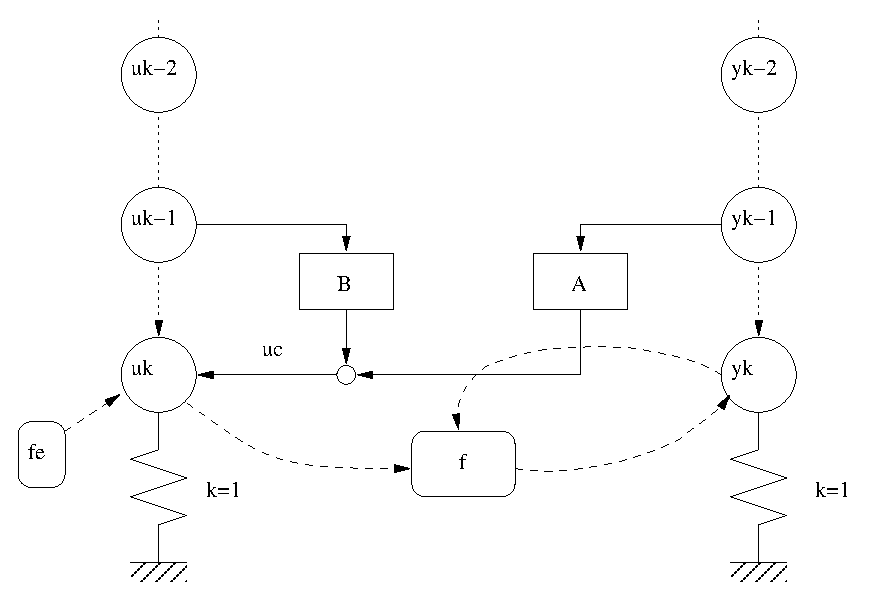
\includegraphics[width=.7\textwidth]{discctrl}
\caption{Discrete control layout.}
\label{fig:discctrl}
\end{figure}

The syntax is
%\begin{verbatim}
\begin{Verbatim}[commandchars=\\\{\}]
    \bnt{electric_type} ::= \kw{discrete control}

    \bnt{electric_arglist} ::= \bnt{num_outputs} , \bnt{num_inputs} ,
        \bnt{order_A} [ , \kw{fir} , \bnt{order_B} ] ,
        \bnt{num_iter} ,
        \bnt{control_data} , 
        \kw{outputs} ,
            (\ty{ScalarValue}) \bnt{output_value}
                [ , \kw{scale} , (\hty{DriveCaller}) \bnt{scale} ]
            [ , ... ] ,
        \kw{inputs} ,
            (\hty{NodeDof}) \bnt{input_dof}
            [ , ... ]

    \bnt{output_value} ::=
        \{ [ \kw{node dof} , ] (\hty{NodeDof}) \bnt{output_dof}
            | \kw{drive} , (\hty{DriveCaller}) \bnt{output_drive} \}
\end{Verbatim}
%\end{verbatim}
The lists of the output and input dofs follows. The inputs
do not require the \nt{order\_A} and \nt{order\_B} fields,
since they are simply used to compute the control forces,
and thus identify an equation.
\nt{order\_B} defaults to \nt{order\_A} unless a \kw{fir} control is chosen.

The \nt{control\_data} has the syntax:
%\begin{verbatim}  
\begin{Verbatim}[commandchars=\\\{\}]
        \bnt{control_data} ::= \bnt{control_type} , \bnt{control_arglist}
\end{Verbatim}
%\end{verbatim}
At present only a simple form of control is implemented. Other types
to come are system identification, both recursive and one-shot, and
adaptive control, with different models and schemes, all based on 
Generalized Predictive Control (GPC) and Deadbeat Control.
The \nt{control\_data} syntax is:
%\begin{verbatim}
\begin{Verbatim}[commandchars=\\\{\}]
    \bnt{control_data} ::=
        \{ \kw{control} , " \bnt{control_matrices_file} "
            | \kw{identification} , \bnt{identification_data}
            | \kw{adaptive control} , \bnt{adaptive_control_data} \}
\end{Verbatim}
%\end{verbatim}

\subsubsection{Control}
The file \nt{control\_matrices\_file} must contain the matrices
$ a_c $, $ b_c $ of the control in plain text (as generated by Matlab, for
instance):

\noindent
\begin{tabular}{l}
    $ a_{c1} $, \\
    \ldots,     \\
    $ a_{cp} $, \\
    $ b_{c1} $, \\
    \ldots,     \\
    $ b_{cp} $  \\
\end{tabular} \\
where $ p $ is the \nt{order\_A} of the controller and the matrices $ a_c $
have \nt{num\_inputs} rows and \nt{num\_outputs} columns, while the
matrices $ b_c $ have \nt{num\_inputs} rows and \nt{num\_inputs} columns.

\subsubsection{Identification}
%\begin{verbatim}
\begin{Verbatim}[commandchars=\\\{\}]
    \bnt{identification_data} ::=
        \{ \kw{arx} | \kw{armax} \}
        [ , \bnt{forgetting_factor} ]
        [ , \bnt{persistent_excitation} ]
        [ , \kw{file} , " \bnt{output_file_name} " ]
\end{Verbatim}
%\end{verbatim}
The forgetting factor is defined as
%\begin{verbatim}
\begin{Verbatim}[commandchars=\\\{\}]
    \bnt{forgetting_factor} ::=
        \kw{forgettingfactor} ,
          \{ \kw{const} , \bnt{d}
              | \kw{dynamic} , \bnt{n1} , \bnt{n2} , \bnt{rho} , \bnt{fact} , \bnt{kref} , \bnt{klim} \}
\end{Verbatim}
%\end{verbatim}
The default is a \kw{const} forgetting factor with $\nt{d}=1$.

The \nt{persistent\_excitation} is defined as
%\begin{verbatim}
\begin{Verbatim}[commandchars=\\\{\}]
    \bnt{persistent_excitation} ::=
        \kw{excitation} , (\hty{DriveCaller}) \bnt{excitation_drive} [ , ... ]
\end{Verbatim}
%\end{verbatim}
where \nt{num\_inputs} instances of \nt{excitation\_drive} must be defined.
By default, no persistent excitation is defined.

\subsubsection{Adaptive control}
The \nt{adaptive\_control\_data} card is
%\begin{verbatim}
\begin{Verbatim}[commandchars=\\\{\}]
    \bnt{adaptive_control_data} ::=
        [ \{ \kw{arx} | \kw{armax} \} , ]
        [ \kw{periodic} , \bnt{periodic_factor} , ]
        \{ \kw{gpc} ,
            \bnt{prediction_advancing_horizon} ,
            \bnt{control_advancing_horizon} ,
            \bnt{prediction_receding_horizon} ,
            [ \kw{prediction weights} , \bnt{Wi} [ , ... ] , ]
            [ \kw{control weights} , \bnt{Ri} [ , ... ] , ]
            (\hty{DriveCaller}) \bnt{weight_drive}
        | \kw{deadbeat} ,
            \bnt{prediction_advancing_horizon} ,
            \bnt{control_advancing_horizon} \}
        [ , \bnt{forgetting_factor} ]
        [ , \bnt{persistent_excitation} ]
        [ , \kw{trigger} , (\hty{DriveCaller}) \bnt{trigger_drive} ]
        [ , \kw{desired output} , (\hty{DriveCaller}) \bnt{output_drive} [ , ... ] ]
        [ , \kw{file} , " \bnt{file_name} " ]
\end{Verbatim}
%\end{verbatim}
The default is \kw{arx}.

The meaning of the keywords is:
\begin{itemize}
\item the \nt{periodic\_factor} defaults to 0;

\item if the keyword \kw{prediction weights} is present,
a number of weights \nt{Wi} equal to
\begin{quote}
$(\nt{prediction\_advancing\_horizon} - \nt{prediction\_receding\_horizon})$
\end{quote}
must be supplied.
If the keyword \kw{control weights} is present,
a number of weights \nt{Ri} equal to \nt{control\_advancing\_horizon}
must be supplied.
If the keywords are not defined, the corresponding weights
default to 1;

\item the \kw{desired output}
option requires \nt{num\_outputs} drives to be defined.
\end{itemize}

\subsubsection{Private Data}
The following data are available:
\begin{enumerate}
\item \kw{"u[\bnt{idx}]"} value of the \nt{idx}-th control output.
\end{enumerate}

\subsubsection{Examples}
Consider the case of a discrete controller that computes
a set of control signals $\T{u}_k$ by adding to their value
at the previous step, $\T{u}_{k-1}$, a contribution coming
from some measure $\T{y}_{k-1}$.
The control matrices are
\begin{subequations}
\begin{align}
	\TT{A}_{c1}
	&=
	\sqbr{\matr{cc}{
		a_{11} & a_{12} \\
		a_{21} & a_{22}
	}}
	\\
	\TT{B}_{c1}
	&=
	\sqbr{\matr{cc}{
		1 & 0 \\
		0 & 1
	}}
\end{align}
\end{subequations}
They are defined in the control data file \texttt{discretecontrol.dat} as
\begin{verbatim}
    a_11 a_12
    a_21 a_22
    1.0 0.0
    0.0 1.0
\end{verbatim}
The model consists in two abstract nodes for the control input
\hty{NodeDof} objects.
They need to be grounded.
This can be formulated by using a \kw{spring support} \kw{genel}
for each \kw{abstract} node, characterized by a unit spring coefficient,
such that
\begin{subequations}
\begin{align}
	1 \cdot x_{u1} &= u_1
	\\
	1 \cdot x_{u2} &= u_2
\end{align}
\end{subequations}
Moreover, assume that the first measure, $y_1$,
comes from a \hty{NodeDof} object,
while the second one, $y_2$, comes from a \hty{DriveCaller} object.
The equation corresponding to $y_1$ must be appropriately grounded
as well, for example by means of yet another \kw{spring support}
\kw{genel}.
This is outside the scope of the present example, so it will assume
the output nodes are defined appropriately.

The model is
\begin{verbatim}
    set: integer U_1 = 1;
    set: integer U_2 = 2;
    set: integer Y_1 = 11;
    # ...
    abstract: U_1;
    abstract: U_2;
    # ...
    genel: U_1, spring support,
        U_1, abstract, algebraic,
        linear elastic, 1.;
    genel: U_2, spring support,
        U_2, abstract, algebraic,
        linear elastic, 1.;
    electric: 99, discrete control,
        2,    # number of `outputs' y
        2,    # number of `inputs' u
        1,    # order of output matrices A (same for input matrices B)
        1,    # update every iteration
        control, "discretecontrol.dat",
        outputs,
            node dof, Y_1, abstract, algebraic, scale, 1.e-3,
            drive, sine, .5, 2*pi, 1., forever, 0, scale, 1.e-3,
        inputs,
            U_1, abstract, algebraic,
            U_2, abstract, algebraic;
\end{verbatim}



\subsection{Displacement}
%\begin{verbatim}
\begin{Verbatim}[commandchars=\\\{\}]
    \bnt{electric_type} ::= \kw{displacement}

    \bnt{electric_arglist} ::=
        \bnt{struct_node_1_label} , (\hty{Vec3}) \bnt{relative_offset_1} ,
        \bnt{struct_node_2_label} , (\hty{Vec3}) \bnt{relative_offset_2} ,
        \bnt{abstract_node_label}
\end{Verbatim}
%\end{verbatim}
\begin{subequations}
\begin{align}
	\T{d} &= \T{x}_b + \T{o}_b - \T{x}_a - \T{o}_a \\
	x &= \sqrt{\T{d}^T \T{d}}
\end{align}
\end{subequations}
The value $x$ is added to the right-hand side of the equation
of the \kw{abstract} node.

\subsection{Motor}
%\begin{verbatim}
\begin{Verbatim}[commandchars=\\\{\}]
    \bnt{electric_type} ::= \kw{motor}

    \bnt{electric_arglist} ::=
        \bnt{struct_node_1_label} ,
        \bnt{struct_node_2_label} ,
        ((\ty{Unit})\hty{Vec3}) \bnt{direction_relative_to_node_1} ,
        \bnt{abstract_node_1_label} ,
        \bnt{abstract_node_2_label} ,
        (\ty{real}) \bnt{dG},
        (\ty{real}) \bnt{dL},
        (\ty{real}) \bnt{dR}
        [ , \kw{initial current} , \bnt{i_0} ]
\end{Verbatim}
%\end{verbatim}
This element implements a simple DC motor, whose equations are
\begin{subequations}
\begin{align}
	\omega &= \T{e}^T \plbr{\T{\omega}_2 - \T{\omega}_1} \\
	V &= V_2 - V_1 \\
	V &= \nt{dL} \frac{\mathrm{d}i}{\mathrm{d}t} + \nt{dR} \, i + \nt{dG} \, \omega \\
	\T{c}_1 &= - \T{e} \, \nt{dG} \, i \\
	\T{c}_2 &= \T{e} \, \nt{dG} \, i \\
	i_1 &= -i \\
	i_2 &= i
\end{align}
\end{subequations}
where \nt{dL} is the inductance, \nt{dR} is the resistance, and \nt{dG} is the motor torque/back-EMF constant.

The motor applies an internal torque, $C = \nt{dG} \, i$, about direction
$\T{e}=\nt{direction\_relative\_to\_node\_1}$, with opposite sign
to both the structural nodes it is connected to, namely \nt{struct\_node\_1\_label} and \nt{struct\_node\_2\_label}.
The input vector that represents direction $\T{e}$ is internally normalized to unity.

It also contributes with a current $i$ to both the electrical nodes it is connected to,
the abstract nodes \nt{abstract\_node\_1\_label} and \nt{abstract\_node\_2\_label}.

The element assumes that the only allowed relative motion between nodes 1 and 2 is a rotation about direction $\T{e}$,
so appropriate joints (e.g.\ a \kw{total joint}, a \kw{revolute hinge}, or \kw{revolute pin}) must be in place.






\section{Force}\label{sec:EL:FORCE}
The \kw{force} element is a general means to introduce 
a right-hand side to the equations, i.e.\ an explicit contribution
to the equations.
There is a basic distinction between abstract and structural forces:
abstract forces apply to arbitrary equations, while structural forces
(and couples) are specific to structural nodes and have
a spatial characterization.
Essentially, structural forces have three components
that may depend on arbitrary parameters (usually the simulated time),
and a location in space.
Structural couples have three parameter-dependent components.
The syntax of the \kw{force} element is:
%\begin{verbatim}
\begin{Verbatim}[commandchars=\\\{\}]
    \bnt{elem_type} ::= \{ \kw{force} | \kw{couple} \}

    \bnt{normal_arglist} ::= \bnt{force_type} , \bnt{force_arglist}

    \bnt{force_type} ::=
        \{ \kw{abstract} [ \kw{internal} ]                                 # \kw{force}
            | \{ \kw{absolute} | \kw{follower} | \kw{total} \} [ \kw{internal} ]      # \kw{force}, \kw{couple}
            | \kw{modal}                                             # \kw{force}
            | \kw{external} \{ \kw{structural} | \kw{modal} \} [ \kw{mapping} ] \}     # \kw{force}
\end{Verbatim}
%\end{verbatim}
The \kw{abstract} \nt{force\_type} applies to generic equations;

The structural force types (\kw{absolute}, \kw{follower}, \kw{total})
only apply to equilibrium equations
related to \kw{structural} nodes.
The \kw{couple} element can only be structural.
It is discussed in this section because of its input syntax commonality 
with the structural \kw{force} elements.

The \kw{modal} \nt{force\_type} applies to equations related
to a \kw{modal} element.

The \kw{external structural} and the \kw{external modal} types
are essentially used to provide an easy to use interface
for coupling with external software in a loose or tight manner.

\subsection{Output}
The output is discussed according to the types of forces. 
The label of the element is output first in all the cases.

\subsection{Abstract force}\label{sec:EL:FORCE:ABSTRACT}
%\begin{verbatim}
\begin{Verbatim}[commandchars=\\\{\}]
    \bnt{elem_type} ::= \kw{force}

    \bnt{force_type} ::= \kw{abstract}

    \bnt{force_arglist} ::=
        (\hty{NodeDof})     \bnt{dof} ,
        (\hty{DriveCaller}) \bnt{force_magnitude}
\end{Verbatim}
%\end{verbatim}
the \nt{dof} field is a normal \hty{NodeDof}; no \kw{order} is required
since the \kw{force} simply applies to the equation related to the node,
regardless of the order.

\subsubsection{Output}
The format is:
\begin{itemize}
    \item the label of the element;
    \item the label of the node\footnote{Since the \kw{abstract} force type
	can connect to \hty{NodeDof}, information provided here
	can be partial if the \hty{NodeDof} actually represents
	a component of a node with more than one degree of freedom.
	\label{footnote:EL:FORCE:ABSTRACT:OUTPUT:node_dof}}
	the force is applied to;
    \item the value of the force.
\end{itemize}

\subsection{Abstract reaction force}
%\begin{verbatim}
\begin{Verbatim}[commandchars=\\\{\}]
    \bnt{elem_type} ::= \kw{force}

    \bnt{force_type} ::= \kw{abstract internal}

    \bnt{force_arglist} ::=
        (\hty{NodeDof})     \bnt{dof_1} ,
        (\hty{NodeDof})     \bnt{dof_2} ,
        (\hty{DriveCaller}) \bnt{force_magnitude}
\end{Verbatim}
%\end{verbatim}
the \nt{dof\_1} and \nt{dof\_2} fields are normal \hty{NodeDof}
but no \kw{order} is required since the \kw{force} simply applies
to the equations related to the nodes, regardless of the order, with
opposite magnitudes.

\subsubsection{Output}
The format is:
\begin{itemize}
    \item the label of the element;
    \item the label of the first node\footnote{See
	footnote~\ref{footnote:EL:FORCE:ABSTRACT:OUTPUT:node_dof}.}
	the force is applied to;
    \item the value of the force applied to the first node;
    \item the label of the second node\footnote{See
	footnote~\ref{footnote:EL:FORCE:ABSTRACT:OUTPUT:node_dof}.}
	the force is applied to;
    \item the value of the force applied to the second node
	  (opposite to that applied to the first node).
\end{itemize}

\subsection{Structural force}
\label{sec:EL:FORCE:STRUCTURAL:FORCE}
%\begin{verbatim}
\begin{Verbatim}[commandchars=\\\{\}]
    \bnt{elem_type} ::= \kw{force}

    \bnt{force_type} ::= \{ \kw{absolute} | \kw{follower} \} 

    \bnt{force_arglist} ::=
        \bnt{node_label} , 
        \kw{position} , (\hty{Vec3}) \bnt{relative_arm} ,
        (\htybty{TplDriveCaller}{Vec3}) \bnt{force_value}

    \bnt{force_type} ::= \kw{total}

    \bnt{force_arglist} ::=
        \bnt{node_label}
        [ , \kw{position} , (\hty{Vec3}) \bnt{relative_arm} ]
        [ , \kw{force orientation} , (\hty{Mat3x3}) \bnt{force_orientation} ]
        [ , \kw{moment orientation} , (\hty{Mat3x3}) \bnt{moment_orientation} ]
        [ , \kw{force} , (\htybty{TplDriveCaller}{Vec3}) \bnt{force_value} ]
        [ , \kw{moment} , (\htybty{TplDriveCaller}{Vec3}) \bnt{moment_value} ]
\end{Verbatim}
%\end{verbatim}
The vector \nt{relative\_arm} defines the offset with respect
to the node of the point where the force is applied.
The drive \nt{force\_value} defines the value of the force
as a function of time.
The \kw{total} force is intrinsically follower.
See also the 
\hyperref{\kw{total joint}}{\kw{total joint} (Section~}{)}{sec:EL:STRUCT:JOINT:TOTAL_JOINT}.

The force and the moment applied to node \nt{node\_label} are thus
\begin{itemize}
\item \kw{absolute} force element:
\begin{subequations}
\begin{align}
	\T{f} & = \nt{force\_value} \\
	\T{m} & = \plbr{\TT{R} \cdot \nt{relative\_arm}} \times \nt{force\_value} ;
\end{align}
\end{subequations}

\item \kw{follower} force element:
\begin{subequations}
\begin{align}
	\T{f} & = \TT{R} \ \nt{force\_value} \\
	\T{m} & = \TT{R} \plbr{\nt{relative\_arm} \times \nt{force\_value}} ;
\end{align}
\end{subequations}

\item \kw{total} force element:
\begin{subequations}
\begin{align}
	\T{f} & = \TT{R} \ \nt{force\_orientation} \cdot \nt{force\_value} \\
	\T{m} & = \TT{R} \lplbr{
		\nt{relative\_arm} \times \plbr{ \nt{force\_orientation} \cdot \nt{force\_value}}
	} \nonumber \\
	& \rplbr{\hphantom{= } \mbox{} +
		\nt{moment\_orientation} \nt{moment\_value}
	};
\end{align}
\end{subequations}

\end{itemize}
$\TT{R}$ is the orientation matrix of the node \nt{node\_label}.

\paragraph{Example.} \
\begin{verbatim}
    force: 10, absolute,
        1000,
            position, .5, 0., 0.,
        1., 0., 0.,
            const, 25.;
    force: 20, follower,
        2000,
            position, null,
        component,
            const, 0.,
            ramp, 10., 0., 1., 0.,
            file, 5, 2;
    force: 30, total,
        2000,
            position, .5, 0., 0.,
            force orientation, eye,
            moment orientation, eye,
        1., 0., 0.,
            const, 25.,
        component,
            const, 0.,
            ramp, 10., 0., 1., 0.,
            file, 5, 2;
\end{verbatim}
\paragraph{Known issues.} \
The direction of a force (a \htybty{TplDriveCaller}{Vec3})
by default is interpreted in the reference frame of the node the force acts upon.
When using the \kw{single} style of \htybty{TplDriveCaller}{Vec3},
one can refer to another reference system (the direction specified by the user
is automatically transformed from that reference frame to the one of the node).
However, this causes an ambiguity when the default \kw{single} specifier is omitted,
rather than explicitly written.
A reference system different from the default one can be specified using the syntax
\begin{Verbatim}[commandchars=\\\{\}]
	\kw{single} , \kw{reference} , \bnt{reference_frame} ,
        	(\hty{Vec3}) \bnt{force_value}
\end{Verbatim}
Note that
\begin{verbatim}
    1., 0., 0.                               # equivalent to single, 1., 0., 0.
\end{verbatim}
and
\begin{verbatim}
    single, 1., 0., 0.                       # equivalent to 1., 0., 0.
\end{verbatim}
are equivalent.
However,
\begin{verbatim}
    reference, global, 1., 0., 0.            # incorrect!
\end{verbatim}
is incorrect; the correct form is
\begin{verbatim}
    single, reference, global, 1., 0., 0.    # correct
\end{verbatim}
Currently, a reference frame different from that of the node cannot be specified
for other styles of template drive caller (e.g.\ the \kw{component} style).


\subsubsection{Output}
The format is:
\begin{itemize}
    \item the label of the element;
    \item the label of the node the force is applied to;
    \item the three components of the force;
    \item the arm of the force, in the global frame (i.e.\ referred
          to point $ \cubr{0,0,0} $ and oriented as the global frame)
\end{itemize}

\subsection{Structural internal force}
\label{sec:EL:FORCE:STRUCTURAL:INTERNAL_FORCE}
%\begin{verbatim}
\begin{Verbatim}[commandchars=\\\{\}]
    \bnt{elem_type} ::= \kw{force}

    \bnt{force_type} ::= \{ \kw{absolute} | \kw{follower} \} \kw{internal}

    \bnt{force_arglist} ::=
        \bnt{node_1_label} , 
        \kw{position} , (\hty{Vec3}) \bnt{relative_arm_1} ,
        \bnt{node_2_label} ,
        \kw{position} , (\hty{Vec3}) \bnt{relative_arm_2} ,
        (\htybty{TplDriveCaller}{Vec3}) \bnt{force_value}

    \bnt{force_type} ::= \kw{total internal}

    \bnt{force_arglist} ::=
        \bnt{node_1_label} ,
        [ \kw{position} , (\hty{Vec3}) \bnt{relative_arm_1} , ]
        [ \kw{force orientation} , (\hty{Mat3x3}) \bnt{force_orientation_1} , ]
        [ \kw{moment orientation} , (\hty{Mat3x3}) \bnt{moment_orientation_1} , ]
        \bnt{node_2_label}
        [ , \kw{position} , (\hty{Vec3}) \bnt{relative_arm_2} ]
        [ , \kw{force orientation} , (\hty{Mat3x3}) \bnt{force_orientation_2} ]
        [ , \kw{moment orientation} , (\hty{Mat3x3}) \bnt{moment_orientation_2} ]
        [ , \kw{force} , (\htybty{TplDriveCaller}{Vec3}) \bnt{force_value} ]
        [ , \kw{moment} , (\htybty{TplDriveCaller}{Vec3}) \bnt{moment_value} ]
\end{Verbatim}
%\end{verbatim}
The format is basically identical to the previous case,
except for the definition of the second node.

\subsubsection{Output}
The format is:
\begin{itemize}
    \item the label of the element;
    \item the label of the first node the force is applied to;
    \item the three components of the force applied to the first node;
    \item the arm of the force with respect to the first node,
	  in the global frame (i.e.\ referred to point $ \cubr{0,0,0} $
	  and oriented as the global frame).
    \item the label of the second node the force is applied to;
    \item the three components of the force applied to the second node
	  (opposite to that applied to the first node);
    \item the arm of the force with respect to the second node,
	  in the global frame (i.e.\ referred to point $ \cubr{0,0,0} $
	  and oriented as the global frame).
\end{itemize}

\paragraph{Example.} \
\begin{verbatim}
    # constant structural force
    force: 1, absolute,
        10, position, null,
        0., 0., 1.,
            const, 100.;

    # constant structural internal force
    force: 1, absolute internal,
        10, position, null,
        20, position, null,
        0.,0.,1.,
            const, 100.;
\end{verbatim}


\subsection{Structural couple}
\label{sec:EL:FORCE:STRUCTURAL:COUPLE}
The structural couple is defined by using \kw{couple} as \nt{elem\_type}.
%\begin{verbatim}
\begin{Verbatim}[commandchars=\\\{\}]
    \bnt{elem_type} ::= \kw{couple}

    \bnt{force_type} ::= \{ \kw{absolute} | \kw{follower} \} 

    \bnt{force_arglist} ::=
        \bnt{node_label} ,
        [ \kw{position} , (\hty{Vec3}) \bnt{relative_arm} , ]
        (\htybty{TplDriveCaller}{Vec3}) \bnt{couple_value}
\end{Verbatim}
%\end{verbatim}
The vector \nt{relative\_arm} defines the offset with respect
to the node of the point where the couple is applied.
It is not used in the analysis (since it makes no sense),
but it can be optionally provided for future reference
(e.g.\ for the visualization of the couple).
The drive \nt{couple\_value} defines the value of the couple
as a function of time.

The moment applied to node \nt{node\_label} is thus
\begin{itemize}
\item \kw{absolute} couple element:
\begin{align}
	\T{m} & = \nt{couple\_value}
\end{align}

\item \kw{follower} couple element:
\begin{align}
	\T{m} & = \TT{R} \cdot \nt{couple\_value}
\end{align}
\end{itemize}
$\TT{R}$ is the orientation matrix of the node \nt{node\_label}.

\subsubsection{Output}
The format is:
\begin{itemize}
    \item the label of the element;
    \item the label of the node the couple is applied to;
    \item the three components of the couple.
\end{itemize}

\subsection{Structural internal couple}
\label{sec:EL:FORCE:STRUCTURAL:INTERNAL_COUPLE}
The structural couple is defined by using \kw{couple} as \nt{elem\_type}.
%\begin{verbatim}
\begin{Verbatim}[commandchars=\\\{\}]
    \bnt{elem_type} ::= \kw{couple}

    \bnt{force_type} ::= \{ \kw{absolute} | \kw{follower} \} \kw{internal}

    \bnt{force_arglist} ::=
        \bnt{node_1_label} ,
        [ \kw{position} , (\hty{Vec3}) \bnt{relative_arm_1} , ]
        \bnt{node_2_label} ,
        [ \kw{position} , (\hty{Vec3}) \bnt{relative_arm_2} , ]
        (\htybty{TplDriveCaller}{Vec3}) \bnt{couple_value}
\end{Verbatim}
%\end{verbatim}
The format is basically identical to the previous case,
except for the definition of the second node.

\subsubsection{Output}
The format is:
\begin{itemize}
    \item the label of the element;
    \item the label of the first node the couple is applied to;
    \item the three components of the couple applied to the first node;
    \item the label of the second node the couple is applied to;
    \item the three components of the couple applied to the second node
	  (opposite to that applied to the first node);
\end{itemize}

\bigskip
Note: by using a \kw{dof}, a \kw{node} or an \kw{element} drive,
a simple feedback control can be easily implemented.
Note however that the dependence of a force on some internal state
does not result in adding the corresponding contribution 
to the Jacobian matrix: the force remains explicit.
Their improper use may result in missing convergence,
or singularity of the Jacobian matrix of the problem.

\subsection{Modal}
%\label{sec:EL:FORCE:MODAL}
\label{sec:ModalJoint}
This element allows to define a set of generalized forces
acting on the equations related to the generalized variables
of a \htmlref{\kw{modal}}{sec:EL:STRUCT:JOINT:MODAL} joint element.
%\begin{verbatim}
\begin{Verbatim}[commandchars=\\\{\}]
    \bnt{elem_type} ::= \kw{force}

    \bnt{force_type} ::= \kw{modal}

    \bnt{force_arglist} ::=
        \bnt{modal_label} ,
            [ \kw{list} , \bnt{number_of_modes} , \bnt{mode1} [ , ... ] , ]
        (\hty{DriveCaller}) \bnt{force1}
            [ , \kw{resultant} , (\hty{Vec3}) \bnt{f} , (\hty{Vec3}) \bnt{m} ]
        [ , ... ]
\end{Verbatim}
%\end{verbatim}
It requires the label of the modal joint it is connected to,
\nt{modal\_label}.
If the optional keyword \kw{list} is given, the number of excited modes
\nt{number\_of\_modes} and the list of the excited modes is expected,
otherwise it assumes all modes of the \nt{modal\_label} modal joint
will be excited.

A list of
\hyperref{\kw{drive callers}}{\kw{drive callers} (see Section~}{)}{sec:DriveCaller}.
that provide the excitation value for each mode is required last.
If the keyword \kw{list} was given, the drive callers
must be \nt{number\_of\_modes}, otherwise they must be as many
as the modes of the excited modal joint element.

If the \kw{modal} joint element is connected to a modal node
instead of being clamped to the ground, the optional keyword \kw{resultant}
is allowed for each mode drive caller.
The keyword \kw{resultant} is followed by two $3\times 1$ vectors
containing the resultant force and moment associated with the related mode.

If the keyword \kw{list} was given, the mode numbers must be
the actual mode numbers defined in the FEM model.

\paragraph{Example.} \
In this example, all the modes available in the FEM data file 
are used by the modal joint, and all the modes are excited
by the modal force
\begin{verbatim}
    joint: MODAL_JOINT, modal, MODAL_NODE,
        5,             # number of modes
        from file,
        "model.fem",
        0;             # no interface nodes
    force: MODAL_FORCE, modal, MODAL_JOINT,
        const, 5.,
        const, 10.,
        const, 1.,
        const, -1.,
        const, -3.;
\end{verbatim}

In this example, only three modes of the same FEM data file
of the previous example are used by the modal joint;
only the last mode is excited by the modal force
\begin{verbatim}
    joint: MODAL_JOINT, modal, MODAL_NODE,
        3,             # number of modes
            list, 1, 3, 5,
        from file,
        "model.fem",
        0;             # no interface nodes
    force: MODAL_FORCE, modal, MODAL_JOINT,
        list, 1,       # only one mode is excited
            5,         # it is mode #5 in "model.fem"
        const, -3.;
\end{verbatim}
Note that the mode is indicated by its number in the FEM data file.




\subsection{External forces}
External forces are elements that allow to communicate
with an external software that computes forces
based on information on the kinematics of the model.

Different communication schemes are supported.
By default, communication occurs via files.
Currently supported communication schemes are
%\begin{verbatim}
\begin{Verbatim}[commandchars=\\\{\}]
    \bnt{external_force_communicator} ::= \{ \bnt{file} | \bnt{edge} | \bnt{socket} \}

    \bnt{file} ::=                             # the default
        " \bnt{input_file_name} " [ , \kw{unlink} ] ,
        " \bnt{output_file_name} " [ , \kw{no clobber} ]
        [ , \bnt{common_parameters} ]

    \bnt{edge} ::= \kw{edge} ,
        " \bnt{flag_file_name} " ,
        " \bnt{data_file_name} "
        [ , \bnt{common_parameters} ]

    \bnt{socket} ::= \kw{socket} ,
        [ \kw{create} , \{ \kw{yes} | \kw{no} \} , ]
        \{ \kw{path} , \bnt{path} | \kw{port} , \bnt{port} [ , \kw{host} , \bnt{host} ] \}
        [ , \bnt{common_parameters} ]

    \bnt{common_parameters} ::= \bnt{common_parameter} [ , ... ]

    \bnt{common_parameter} ::=
        \{ \kw{sleep time} , \bnt{sleep_time}
            | \kw{precision} , \{ \kw{default} | \bnt{digits} \}   # not valid for \kw{socket}
            | \kw{coupling} , \{ \kw{staggered} | \kw{loose} | \kw{tight} | \bnt{coupling_steps} \}
            | \kw{send after predict} , \{ \kw{yes} | \kw{no} \} \}
\end{Verbatim}
%\end{verbatim}

\subsubsection{File communicator}
\nt{input\_file\_name} is the name of the file MBDyn expects to find
with the values of the force.
The content depends on the purpose it is used for.
The optional keyword \kw{unlink} indicates that MBDyn is supposed
to unlink the file as soon as it is ready to read another one,
as a primitive form of inter-process communication.

\nt{output\_file\_name} is the name of the file MBDyn creates
each time it intends to communicate the kinematics of the model
to the external software.
The contents depend on the purpose it is used for.
The option \kw{no clobber} indicates that MBDyn is supposed to wait
until the external software removed the file before generating a new one,
as a primitive form of inter-process communication.



\subsubsection{EDGE communicator}
This communicator has been developed in cooperation with Luca Cavagna,
to support communication with FOI's EDGE.

The file \nt{flag\_file\_name} is used to synchronize the communication
between the processes.
The same file is truncated and reused by both processes.
The syntax of the file changed since EDGE 5.1; this change is reflected
from MBDyn 1.3.16 on.
The file contains a two lines header, followed by a line containing a single digit.
The header is
\begin{verbatim}
    UPDATE,N,0,0,1
    FLAG,I,1,1,0
\end{verbatim}
The digit indicates the command.  Its meaning is:
\begin{itemize}
\item[0 :] external software is initializing; MBDyn must wait;
\item[1 :] external software is busy; MBDyn must wait;
\item[2 :] external software is ready to read kinematics; MBDyn can start reading forces and writing kinematics;
\item[3 :] MBDyn finished writing kinematics; external software can start reading kinematics and writing forces
	(written by MBDyn when data file is ready);
\item[4 :] external software converged; MBDyn should go to convergence, advance to the next time step,
and start writing new step kinematics;
\item[5 :] external software decided to quit; MBDyn should stop communicating.
\end{itemize}
So far, there are no provisions for re-executing a time step,
nor for communicating either the time or the time step,
so adaptive time stepping cannot be implemented.

\nt{data\_file\_name} is the name of the file used to actually send data
between the two processes.
Its contents depend on the purpose it is used for,
as described in the subsequent sections.



\subsubsection{Socket communicator}
\label{sec:el:forces:comm:socket}
The optional parameter \kw{create}, when set to \kw{yes}, indicates
that MBDyn will create the socket, and the peer will have to connect to it.
Otherwise, when set to \kw{no}, it indicates that MBDyn will try to connect
to an already existing socket created by the peer.
Connecting to a peer is attempted while reading the input file.
Sockets are created when the input file has been read.
MBDyn waits until all sockets have been connected to by peers
before the simulation is started.

MBDyn supports local (unix) sockets, defined using the \kw{path} parameter,
and inet sockets, defined using the \kw{port} parameter.
When \kw{create} is set to \kw{yes}, the optional keyword \kw{host}
allows to define what interface MBDyn will listen on.
When \kw{create} is set to \kw{no}, the optional keyword \kw{host}
indicates what host to connect to.
It defaults to `localhost'.




\subsubsection{Common parameters}
The optional parameter \nt{sleep\_time} determines how long MBDyn
is supposed to sleep while waiting for a new input file to appear
or for an old output file to disappear.

The optional parameter \nt{precision} determines the precision
used in writing the output file; the default is 16 digits.
This is only meaningful for communicators based on textual files.

The optional parameter \kw{coupling} determines whether the coupling
will be \kw{staggered} (communicate each time step, with one step delay),
\kw{loose} (communicate each time step, no delay, the default) or
\kw{tight} (communicate each iteration); otherwise, if \nt{coupling\_steps}
is provided, the communication occurs every \nt{coupling\_steps}.

The optional parameter \kw{send after predict} allows to indicate
whether MBDyn must send the predicted motion or not when playing
a tight coupling loop.


\paragraph{Staggered Coupling.} \
When the coupling is \kw{staggered}, the communication pattern is:
\begin{enumerate}
\item MBDyn receives a set of forces sent by the external peer
	the first time the residual is assembled within time step $k$;
	the external peer generated that set of forces
	based on the kinematics at step $k-1$;

\item MBDyn sends a set of kinematic parameters related to step $k$
	after convergence.
\end{enumerate}
As a consequence, MBDyn solves the kinematics at the current time step, $k$,
using forces evaluated for the kinematics at the previous time step, $k-1$.
Something like
\begin{align}
	\T{f}\plbr{\T{y}_k, \dot{\T{y}}_k, \T{u}_{k - 1}}
	&=
	\T{0}
	.
\end{align}
Note: not implemented yet.

\paragraph{Loose Coupling.} \
When the coupling is \kw{loose}, the communication pattern is:
\begin{enumerate}
\item MBDyn sends a set of kinematic parameters related to step $k$
	after predict.

\item MBDyn receives a set of forces sent by the external peer
	the first time the residual is assembled within time step $k$;
	the external peer generated that set of forces
	based on the predicted kinematics at step $k$;
\end{enumerate}
As a consequence, MBDyn solves the kinematics at the current time step, $k$,
using forces evaluated for the predicted kinematics at the current time step, $k$.
Something like
\begin{align}
	\T{f}\plbr{\T{y}_k, \dot{\T{y}}_k, \T{u}_{k}^{(0)}}
	&=
	\T{0}
	.
\end{align}

\paragraph{Tight Coupling.} \
When the coupling is \kw{tight}, the communication pattern is:
\begin{enumerate}
\item MBDyn sends the predicted kinematics for step $k$
	during the ``after predict'' phase
	(unless \kw{send after predict} is set to \kw{no});

\item MBDyn receives a set of forces sent by the external peer
	each time the residual is assembled; those forces are computed
	based on the kinematics at iteration $j$

\item as soon as, while reading the forces, MBDyn is informed that
	the external peer converged, it continues iterating until
	convergence using the last set of forces it read.

%\item if coupling only occurs every some iterations, MBDyn sends
%	a set of kinematic parameters after convergence.
\end{enumerate}
As a consequence, MBDyn solves the kinematics at the current time step, $k$,
at iteration $j$,
using forces evaluated for the kinematics at the same time step, $k$,
but at iteration $j-1$.
Something like
\begin{align}
	\T{f}\plbr{\T{y}_k^{(j)}, \dot{\T{y}}_k^{(j)}, \T{u}_k^{(j-1)}}
	&=
	\T{0}
	.
\end{align}




\subsection{External Structural}
\label{sec:EL:FORCE:EXTERNAL:STRUCTURAL}
This element allows to communicate with an external software that computes
forces applied to a pool of nodes and may depend on the kinematics of those
nodes.
Communication occurs by means of the communicators illustrated earlier.
%\begin{verbatim}
\begin{Verbatim}[commandchars=\\\{\}]
    \bnt{elem_type} ::= \kw{force}

    \bnt{force_type} ::= \kw{external structural}

    \bnt{force_arglist} ::= \bnt{external_force_communicator} ,
        [ \kw{reference node} , \bnt{ref_node_label} , ]
        [ \{ \kw{labels} , \{ \kw{yes} | \kw{no} \}
                | \kw{sorted} , \{ \kw{yes} | \kw{no} \}
                | \kw{orientation} ,
                    \{ \kw{none} | \kw{orientation matrix} | \kw{orientation vector} | \kw{euler 123} \}
                | \kw{accelerations} , \{ \kw{yes} | \kw{no} \}
                | \kw{use reference node forces} , \{ \kw{yes} | \kw{no} \}
                    [ , \kw{rotate reference node forces} , \{ \kw{yes} | \kw{no} \} ] \}
            [ , ... ] , ]
        \bnt{num_nodes} ,
            \bnt{node_label} [ , \kw{offset} , (\hty{Vec3}) \bnt{offset} ]
            [ , ... ]
        [ , \kw{echo} , \bnt{echo_file_name} ]
\end{Verbatim}
%\end{verbatim}
\begin{itemize}
\item \kw{use reference node forces} only meaningful
when \kw{reference node} is used.
It assumes the external solver is sending the forces and moments
related to the reference node.
They correspond to the rigid-body forces and moments applied
to the whole system.
As such, the forces and moments applied to each node
are removed accordingly.
If it is set to \kw{no}, reference node forces and moments
will be ignored.

\item The orientation style \kw{none} implies that only positions, velocities 
and accelerations will be output (the latter only if \kw{accelerations}
is set to \kw{yes}).

\item \kw{echo} causes the output of the reference configuration
to be produced in a file called \nt{echo\_file\_name}.
If the file exists, it is overwritten, if allowed by file system permissions.
The format is that of the communicator in stream form.
\end{itemize}


\subsubsection{File communicator}
The forces are read from the input file in textual form,
each line formatted as follows:
\begin{itemize}
\item a label (if \kw{labels} is set to \kw{yes});
\item three components of force in the global frame;
\item three components of moment in the global frame,
	referred to the node as the pole.
\end{itemize}
The label indicates what node the force and the moment apply to; 
each force is applied in a point that may be optionally offset 
from the corresponding node location according to \kw{offset}.
If optional keyword \kw{sorted} is set to \kw{no}, the forces might be
read in arbitrary order, so they need to be recognized by the label.
The option \kw{sorted} is only meaningful when \kw{labels} is set to \kw{yes}.

The kinematics are written to the output file in textual form,
each line formatted as follows:
\begin{itemize}
\item a label (if \kw{labels} is set to \kw{yes});
\item the position in the global frame;
\item the orientation of the node with respect to the global frame:
\begin{itemize}
	\item if \kw{orientation} is set to \kw{orientation matrix},
	the orientation matrix in the global frame, row-oriented:
	$R_{11}$, $R_{12}$, $R_{13}$, $R_{21}$, \ldots, $R_{32}$, $R_{33}$;
	\item if \kw{orientation} is set to \kw{orientation vector},
	the orientation vector's components;
	\item if \kw{orientation} is set to \kw{euler 123},
	the three Euler angles, in degrees, according to the 1,2,3
	convention;
\end{itemize}
\item the velocity with respect to the global frame;
\item the angular velocity with respect to the global frame.
\end{itemize}
If the optional keyword \kw{accelerations} is set to \kw{yes},
at the end of each line the following optional fields will appear:
\begin{itemize}
\item the acceleration with respect to the global frame;
\item the angular acceleration with respect to the global frame.
\end{itemize}
The label indicates what node the kinematics is related to;
the position and the velocity refer to a point that may be optionally
offset from the node location according to \kw{offset}.

If a \kw{reference node} was given, the first record is related
to the reference node itself.
The following records contain forces and moments in the reference frame
of the reference node.



\subsubsection{EDGE communicator}
TBD




\subsubsection{Socket communicator}
TBD




\paragraph{Example.} \
The following defines an \kw{external structural} force
with the file communicator
\begin{verbatim}
    set: integer FORCE_LABEL = 1000;
    set: integer NODE_1 = 10;
    set: integer NODE_2 = 20;
    force: FORCE_LABEL, external structural,
        "IN.dat", unlink,
        "OUT.dat", no clobber,
        sleep time, 10,
        precision, 12,
        coupling, loose,
        2, # number of nodes
            NODE_1,
            NODE_2, offset, 0.,0.,.5;
\end{verbatim}

\subsubsection{Output}
An external structural element writes one line for each connected node
at each time step in the \texttt{.frc} file.
Each line contains:
\begin{itemize}
\item in column 1 the label of the element and that of the corresponding node;
	the format of this field is \nt{element\_label}\texttt{@}\nt{node\_label};
\item in columns 2--4 the three components of the force;
\item in columns 5--7 the three components of the moment.
\end{itemize}
If a reference node is defined, a special line is output for the reference node,
containing:
\begin{itemize}
\item in column 1 the label of the element and that of the corresponding node;
	the format of this field is \nt{element\_label}\texttt{\#}\nt{node\_label};
\item in columns 2--4 the three components of the force applied to the reference node,
	as received from the peer;
\item in columns 5--7 the three components of the moment applied to the reference node,
	as received from the peer.
\item in columns 8--10 the three components of the force that are actually applied to the reference node,
	in the global reference frame;
\item in columns 11--13 the three components of the moment
	with respect to the reference node that are actually applied to the reference node,
	in the global reference frame;
\item in columns 14--16 the three components of the force resulting from the combination
	of all nodal forces, in the global reference frame;
\item in columns 17--19 the three components of the moment
	with respect to the reference node resulting from the combination
	of all nodal forces and moments, in the global reference frame;
\end{itemize}




\subsection{External structural mapping}
\label{sec:EL:FORCE:EXTERNAL:STRUCTURAL_MAPPING}
This element allows to communicate with an external software that computes
forces applied to a pool of nodes and may depend on the kinematics of those
nodes through a linear mapping.
Communication occurs by means of the communicators illustrated earlier.
%\begin{verbatim}
\begin{Verbatim}[commandchars=\\\{\}]
    \bnt{elem_type} ::= \kw{force}

    \bnt{force_type} ::= \kw{external structural mapping}

    \bnt{force_arglist} ::= \bnt{external_force_communicator} ,
        [ \kw{reference node} , \bnt{ref_node_label} , ]
        [ \{ \kw{labels} , \{ \kw{yes} | \kw{no} \}
                | \kw{orientation} ,
                    \{ \kw{none} | \kw{orientation matrix} | \kw{orientation vector} | \kw{euler 123} \}
                | \kw{accelerations} , \{ \kw{yes} | \kw{no} \}
                | \kw{use reference node forces} , \{ \kw{yes} | \kw{no} \}
                    [ , \kw{rotate reference node forces} , \{ \kw{yes} | \kw{no} \} ] \}
            [ , ... ] , ]
        \bnt{num_points} ,
            \bnt{node_label} , \kw{offset} [ , \bnt{point_label} ] , (\hty{Vec3}) \bnt{offset}
                [ , ... ]
        [ , \kw{echo} , " \bnt{echo_file_name} "
            [ , \{ \kw{precision} , \bnt{digits}
                    | \kw{surface} , " \bnt{surface_file_name} "
                    | \kw{output} , " \bnt{output_file_name} "
                    | \kw{order} , \bnt{order}
                    | \kw{basenode} , \bnt{basenode}
                    | \kw{weight} , \{ \kw{inf} | (\ty{real}) \bnt{weight} \} \}
                [ , ... ] ]
            [ , \kw{stop} ] ]
        [ , \kw{mapped points number} , \{ \kw{from file} | \bnt{mapped_points} \} ,
            \{ \kw{full} | \kw{sparse} \} \kw{mapping file} , " \bnt{mapping_file_name} "
                [ , \kw{threshold} , \bnt{threshold} ]
            [ , \{ \kw{mapped labels file} , " \bnt{mapped_labels_file_name} "
                | \bnt{mapped_label} [ , ... ] \} ] ]
\end{Verbatim}
%\end{verbatim}
A set of \nt{num\_points} points is generated first,
by computing the kinematics of the points originating
from the rigid-body motion of the structural nodes \nt{node\_label}
according to the specified offset.
Multiple \kw{offset} blocks can appear for each \nt{node\_label}.

The \kw{echo} keyword causes the positions of those points
to be written in a file named \nt{echo\_file\_name}.
If the keyword \kw{stop} is present, the simulation ends here.
This is useful to generate the bulk data that is needed to compute
the linear mapping matrix.
The optional keyword \kw{precision} allows to set \nt{precision}
digits in the logged data; the other optional keywords refer to values
that are written verbatim to the file.
In detail, \nt{surface\_file\_name} is the name of the file that contains
the coordinates of the peer's points, \nt{output\_file\_name}
is the name of the file that will contain the mapping matrix,
\nt{order} is an integer ($1 \le \nt{order} \le 3$),
\nt{basenode} is the number of nodes for each region ($\nt{basenode} > 0$),
\nt{weight} is a weighting coefficient ($\nt{weight} \ge -2$ or \kw{inf})

When the \kw{reference node} keyword is present, the kinematics
of the points is formulated in the reference frame of node
\nt{ref\_node\_label}.
The forces are expected in the same reference frame.
In this case, if \kw{use reference node forces} is set to \kw{yes},
the force and moment related to node \nt{ref\_node\_label} 
returned by the external solver are used;
if \kw{rotate reference node forces} is set to \kw{yes},
they are first rotated in the global reference frame.

When the \kw{mapped points number} keyword is present,
a mapping matrix is read from the file named \nt{mapping\_file\_name}
(same as \nt{output\_file\_name} when the \kw{echo} keyword is used).
If the keyword \kw{from file} is used, the number of \nt{mapped\_points}
is computed from the number of rows of the matrix
in file \nt{mapping\_file\_name}.
The matrix must be
$(3 \times \nt{mapped\_points}) \times (3 \times \nt{num\_points})$.
If the \kw{mapped points number} keyword is not present,
the element behaves as if the mapping were the identity matrix,
namely the position and the velocity of the points rigidly offset
from MBDyn's nodes are directly passed to the peer solver.
See the \htmlref{\kw{modal}}{sec:EL:FORCE:EXTERNAL:MODAL_MAPPING}
variant for a description of the mapping file format.

The labels of the original points, indicated as \nt{point\_label},
and the labels of the mapped points, either contained
in the \nt{mapped\_labels\_file\_name},
or directly listed as \nt{mapped\_label}, must be provided
when \kw{labels} is set to \kw{yes}.



\paragraph{Mapping.} \
The mapping consists in a constant matrix that allows to compute
the position and the velocity of the mapped points (subscript `peer')
as functions of a set of points rigidly offset from MBDyn's nodes
(subscript `mbdyn'),
\begin{subequations}
\begin{align}
	\T{x}_\text{peer}
	&=
	\TT{H} \T{x}_\text{mbdyn}
	\\
	\dot{\T{x}}_\text{peer}
	&=
	\TT{H} \dot{\T{x}}_\text{mbdyn}
\end{align}
\end{subequations}
The same matrix is used to map back the forces onto MBDyn's nodes
based on the preservation of the work done in the two domains,
\begin{align}
	\delta\T{x}_\text{mbdyn}^T \T{f}_\text{mbdyn}
	&=
	\delta\T{x}_\text{peer}^T \T{f}_\text{peer}
	=
	\delta\T{x}_\text{mbdyn}^T \TT{H}^T \T{f}_\text{peer}
\end{align}
which implies
\begin{align}
	\T{f}_\text{mbdyn}
	&=
	\TT{H}^T \T{f}_\text{peer}
\end{align}
To compute matrix $\TT{H}$ one needs to:
\begin{enumerate}
\item gather the coordinates of the set of points used by the peer process
(subscript `peer' in the formulas above) in a file, formatted as
\begin{Verbatim}[commandchars=\\\{\}]
\bnt{num_points}
\bnt{x_1} \bnt{y_1} \bnt{z_1}
...
\bnt{x_n} \bnt{y_n} \bnt{z_n}
\end{Verbatim}
If \kw{reference node} is defined, the points need to be expressed
in a reference frame coincident with that of node \nt{ref\_node\_label}.

\item execute MBDyn's input file after uncommenting the \kw{echo} line
in the definition of the external structural mapping force element,
terminated by the \kw{stop} keyword, to generate the \nt{echo\_file\_name}
file with MBDyn's points coordinates (subscript `mbdyn' in the formulas above).

\item start \texttt{octave}

\item make sure the folder \texttt{contrib/MLS/} is in octave's path
\begin{Verbatim}[commandchars=\\\{\}]
    addpath('/path/to/contrib/MLS')
\end{Verbatim}

\item execute the \texttt{create\_mls\_interface} function
\begin{Verbatim}[commandchars=\\\{\}]
    create_mls_interface('\nt{echo_file_name}');
\end{Verbatim}
This generates the mapping matrix $\TT{H}$, using the files \nt{echo\_file\_name}
and \nt{surface\_file\_name} (the latter is written in \nt{echo\_file\_name}
by the \kw{surface} keyword). The matrix is stored in the file \nt{output\_file\_name}.
The \kw{sparse} storage is recommended, since for usual problems
the matrix is significantly sparse.
\\
\emph{NOTE: this operation can take minutes when the mapped domains consist
of thousands of points.}

\item comment the \kw{echo} line
in the definition of the external structural mapping force element.
\end{enumerate}
From this point on, when MBDyn is executed it loads the mapping matrix
from file \nt{output\_file\_name} using sparse storage, automatically
ignoring coefficients whose absolute value is below \nt{threshold}
(defaults to 0).

The parameters of the mapping, as documented in
\texttt{create\_mls\_interface}, are
\begin{verbatim}
% function create_mls_interface([inputfilename])
%       inputfilename [optional argument] string that contains the name
%       of the file created by the MBDyn external mapping force element 
%       using the "echo" option
%       Additional rows must be either added in the comment section of the file
%       or can be enforced using the appropriate options of the "echo" keyword
%       if input values different from default are required. In detail
%
%       # surface: ...
%               used to indicate the name of the file that contains 
%               the external element grid data. Default: 'surface.dat' 
%
%       # order: used to indicate the polynomial order of the base used by MLS
%               The value must be in the range [1,3]. Default is 2
%
%       # basenode: number of nodes included in the local MLS support
%               should be higher than 0
%
%       # weight: continuity order of the RBF weight function
%               The value must be in the range [-2,inf]
%               -1 means constant weight == 1 in the support
%               -2 means a special weight function == 0 @ the query point 
%               default 2
%
%       # output: name of the file where the interface matrix is saved in sparse format
\end{verbatim}



\paragraph{Example.} \
\begin{verbatim}
    force: 100, external structural mapping,
        socket,
            create, yes,
            path, "/tmp/mbdyn.sock",
            no signal,
        coupling, tight,
        reference node, 0,
        points number, 9,
            10,
                offset, null,       # centered at node
                offset, 0., 1., 0., # y offset
                offset, 0., 0., 1., # z offset
            20,
                offset, null,       # ...
                offset, 0., 1., 0.,
                offset, 0., 0., 1.,
            30,
                offset, null,
                offset, 0., 1., 0.,
                offset, 0., 0., 1.,
        # NOTE: uncomment the line below to generate data required for the mapping
        # echo, "points.dat", surface, "surf.dat", output, "mapping.dat", stop,
        mapped points number, 27,
        sparse mapping file, "mapping.dat";
\end{verbatim}

\subsubsection{File communicator}
TBD

\subsubsection{EDGE communicator}
TBD

\subsubsection{Socket communicator}
TBD

The format of the socket communicator is relatively simple;
however, implementors may exploit the peer library \texttt{libmbc},
whose C API is defined in \texttt{mbc.h}.
A C++ wrapper is defined in \texttt{mbcxx.h}.
A python wrapper is also available.

\subsubsection{Output}
TBD



\subsection{External modal}
\label{sec:EL:FORCE:EXTERNAL:MODAL}
This element allows to communicate with an external software that computes
forces applied to a 
\htmlref{\kw{modal}}{sec:EL:STRUCT:JOINT:MODAL} joint element,
and may depend on the values of the corresponding generalized variables.
Communication occurs by means of the communicators illustrated earlier.
%\begin{verbatim}
\begin{Verbatim}[commandchars=\\\{\}]
    \bnt{elem_type} ::= \kw{force}

    \bnt{force_type} ::= \kw{external modal}

    \bnt{force_arglist} ::= \bnt{external_force_communicator} ,
        \bnt{modal_label}
        [ , \kw{accelerations} ]
        [ , \kw{type} , \{ \kw{rigid} | \kw{modal} | \kw{all} \} ]
\end{Verbatim}
%\end{verbatim}
\nt{modal\_label} is the label of the 
\htmlref{\kw{modal}}{sec:EL:STRUCT:JOINT:MODAL} joint element
the force element is connected to.

If the optional keyword \kw{accelerations} is present,
the output will also contain the modal accelerations.

If the optional keyword \kw{type} is present,
the mutually exclusive keywords \kw{rigid}, \kw{modal} or \kw{all}
inform MBDyn about whether only the rigid or the modal portions
of the force are expected.
The default is \kw{all}, but some communicators might require
a specific value.
If \kw{rigid} or \kw{all} are used, the \kw{modal} joint element
must be connected to a \kw{modal} node.
The number of modes of the modal force must match that of the active modes
in the \kw{modal} joint element.



\subsubsection{File communicator}
If \kw{type} is \kw{rigid} or \kw{all}, the first line of the input file
must contain:
\begin{itemize}
\item the label of the \kw{modal} node the \kw{modal} joint element
	is connected to, or 0 if the element is grounded;
\item three components of force in the \kw{modal} node reference frame;
\item three components of moment in the \kw{modal} node reference frame.
\end{itemize}
If the \kw{modal} joint element is grounded, the force and moment
are ignored.
If \kw{type} is \kw{modal} or \kw{all},
each of the following lines contains the value of the generalized force
for the respective mode.

The output file file is written in textual form.
If \kw{type} is \kw{rigid} or \kw{all}, the first line contains:
\begin{itemize}
\item the label of the \kw{modal} node the \kw{modal} joint element
	is connected to, or 0 if the element is grounded;
\item the position in the global frame;
\item the orientation matrix in the global frame;
\item the velocity with respect to the global frame;
\item the angular velocity with respect to the global frame.
\end{itemize}
If the optional keyword \kw{accelerations} is present,
at the end of each line the following optional fields will appear:
\begin{itemize}
\item the acceleration with respect to the global frame;
\item the angular acceleration with respect to the global frame.
\end{itemize}
If the \kw{modal} joint element is grounded, all the data corresponds
to that of the origin of the global reference frame.
If \kw{type} is \kw{modal} or \kw{all}, each of the following lines contains,
for each mode:
\begin{itemize}
\item the value of the generalized variable;
\item the value of the first derivative of the generalized variable.
\end{itemize}
If the optional keyword \kw{accelerations} is present,
at the end of each line the following optional field will appear:
\begin{itemize}
\item the value of the second derivative of the generalized variable.
\end{itemize}



\subsubsection{EDGE communicator}
When the \kw{edge} communicator is used,
the \kw{accelerations} keyword is ignored.
\kw{type} must be either \kw{rigid} or \kw{modal}.
If both need to be used, two \kw{external modal} forces must be instantiated:
one with \kw{type} set to \kw{rigid}
and the other with \kw{type} set to \kw{modal}.

\paragraph{Rigid.} \
When \kw{type} is \kw{rigid}, the data file written by the external software
is expected to contain:
%\begin{verbatim}
\begin{Verbatim}[commandchars=\\\{\}]
* this is a comment
body_forces,R,1,6,0
\bnt{fx} \bnt{fy} \bnt{fz} \bnt{mx} \bnt{my} \bnt{mz}
\end{Verbatim}
%\end{verbatim}
where \nt{fx}, \nt{fy}, \nt{fz}, \nt{mx}, \nt{my}, \nt{mz}
respectively are the force and moment components
oriented according to the global reference frame.
The moments are referred to the point that represents the origin
of the FE model reference frame, or to either of
the \kw{origin position} or the \kw{origin node} of the \kw{modal} element,
if defined.

The data file written by MBDyn contains:
%\begin{verbatim}
\begin{Verbatim}[commandchars=\\\{\}]
* this is a comment
body_dynamics,N,0,0,3
* Body linear velocity in body axes
VRELV,R,1,3,0
\bnt{vx} \bnt{vy} \bnt{vz}
* Body angular velocity in body axes
VRELM,R,1,3,0
\bnt{omegax} \bnt{omegay} \bnt{omegaz}
* Body reference frame cosines (listed by columns)
OMGMAN,R,3,3,0
\bnt{R11} \bnt{R21} \bnt{R31}
\bnt{R12} \bnt{R22} \bnt{R32}
\bnt{R13} \bnt{R23} \bnt{R33}
\end{Verbatim}
%\end{verbatim}
where:
\begin{itemize}
\item \nt{vx}, \nt{vy}, \nt{vz} are the components of the velocity
	of the rigid body, in body axes;
\item \nt{omegax}, \nt{omegay}, \nt{omegaz} are the components
	of the angular velocity of the rigid body, in body axes;
\item \nt{R11}, \nt{R12}, \nt{R13}, \nt{R21}, \nt{R22}, \nt{R23},
	\nt{R31}, \nt{R32}, \nt{R33} are the components
	of the orientation matrix.
\end{itemize}

\paragraph{Modal.} \
When \kw{type} is \kw{modal}, the external software is expected to write
a data file containing:
%\begin{verbatim}
\begin{Verbatim}[commandchars=\\\{\}]
* this is a comment
modal_force_flow,R,\bnt{n},1,0
\bnt{f1} ... \bnt{fn}
\end{Verbatim}
%\end{verbatim}
where \nt{n} is the number of modes (must match the number of active modes
in the \kw{modal} joint element), while \nt{f1} to \nt{fn} are the amplitudes
of the modal forces.

The data file written by MBDyn contains:
%\begin{verbatim}
\begin{Verbatim}[commandchars=\\\{\}]
* this is a comment
modal_state,N,0,0,2
modal_coordinate,R,1,\bnt{n},0
\bnt{q1} ... \bnt{qn}
modal_velocity,R,1,\bnt{n},0
\bnt{qp1} ... \bnt{qpn}
\end{Verbatim}
%\end{verbatim}
where:
\begin{itemize}
\item \nt{n} is again the number of modes;
\item \nt{q1} to \nt{qn} are the amplitudes of the modal coordinates;
\item \nt{qp1} to \nt{qpn} are the amplitudes of the derivatives
	of the modal coordinates.
\end{itemize}

Each field can be separated by an arbitrary amount of whitespace,
and by at most one ``comma'' (``,'').
Although specifically developed for ease of interfacing with EDGE,
this format is open, and thus can be implemented by other software
in order to easily couple with MBDyn.



\subsubsection{Socket communicator}
When the \kw{socket} communicator is used,
the communication layer is established according to the definition
provided at page~\pageref{sec:el:forces:comm:socket}.
For a single external modal force with \kw{socket} communicator,
\kw{type} can be any of \kw{rigid}, \kw{modal}, or \kw{all}.

\paragraph{Example.} \
\begin{verbatim}
    force: 10, external modal,
        socket,
            create, yes,
            path, "/tmp/mbdyn.sock",
            no signal,
        coupling, tight,
        2;    # modal joint label
\end{verbatim}


\subsubsection{Output}
An external modal element writes multiple lines at each time step
in the \texttt{.frc} file.

If \kw{type} is \kw{ridig} or \kw{all}, the line contains:
\begin{itemize}
\item in column 1 the label of the element and that of the corresponding node;
	the format of this field is \nt{element\_label}\texttt{\#}\nt{node\_label};
\item in columns 2--4 the three components of the force;
\item in columns 5--7 the three components of the moment.
\end{itemize}
If \kw{type} is \kw{modal} or \kw{all}, each line contains:
\begin{itemize}
\item in column 1 the label of the element and the corresponding mode;
	the format of this field is \nt{element\_label}\texttt{.}\nt{mode\_number};
\item in column 2 the amplitude of the corresponding modal force.
\end{itemize}



\subsection{External modal mapping}
\label{sec:EL:FORCE:EXTERNAL:MODAL_MAPPING}
This element allows to communicate with an external software that computes
forces applied to a set of structural nodes,
and may depend on the values of the corresponding variables.
Modal forces are actually computed, based on the value of modal variables.
The element thus projects the motion of the set of structural nodes
in the space of a set of modes before communicating it to the peer.
Similarly, it receives generalized forces that are projected back
in the space of the structural nodes before assembly.
Communication occurs by means of the communicators illustrated earlier
for the \kw{external modal} case.
%\begin{verbatim}
\begin{Verbatim}[commandchars=\\\{\}]
    \bnt{elem_type} ::= \kw{force}

    \bnt{force_type} ::= \kw{external modal mapping}

    \bnt{force_arglist} ::= \bnt{external_force_communicator} ,
        [ \kw{reference node} , \bnt{ref_node_label} , ]
        [ \kw{use rigid body forces} , \{ \kw{yes} | \kw{no} \} ,
            [ \kw{rotate rigid body forces} , \{ \kw{yes} | \kw{no} \} , ] ]
        [ \kw{accelerations} , \{ \kw{yes} | \kw{no} \} , ]
        [ \kw{type} , \{ \kw{rigid} | \kw{modal} | \kw{all} \} , ]
        \kw{nodes number} , \bnt{num_nodes} ,
            \bnt{node_1_label} [ , ... ] ,
        \kw{modes number} , \{ \kw{from file} | \bnt{num_modes} \} ,
        \{ \kw{full} | \kw{sparse} \} \kw{mapping file} , " \bnt{mapping_file_name} "
            [ , \kw{threshold} , \bnt{threshold} ]
            [ , \kw{transpose} ]
\end{Verbatim}
%\end{verbatim}
\nt{ref\_node\_label} is the label of the reference node
if the modes express the motion relative to a specific node.

The mapping file contains the matrix that maps the nodal and modal
displacements, velocities and forces.
When \kw{full mapping file} is used, a file containing
$\nt{num\_modes} \times (6\times\nt{num\_nodes})$ coefficients is expected.

When the optional \kw{transpose} keyword is used, the file is expected to contain
the same number of coefficients, but organized as $(6\times\nt{num\_nodes}) \times \nt{num\_modes}$ coefficients.

When \kw{sparse mapping file} is used, a file containing
%\begin{verbatim}
\begin{Verbatim}[commandchars=\\\{\}]
\bnt{row} \bnt{col} \bnt{value}
\end{Verbatim}
%\end{verbatim}
triplets is expected, with $1 \le \nt{row} \le \nt{num\_modes}$
and $1 \le \nt{col} \le 6\times\nt{num\_nodes}$.
Both files may start with an arbitrary number of lines beginning
with a hash mark (`\texttt{\#}').
They are treated as comments and ignored.

If a \kw{threshold} is given, only elements whose absolute value
is larger than threshold are retained.
The value of \nt{threshold} defaults to 0.

The mapping matrix is internally stored and handled as sparse,
regardless of the file format.

When the keyword \kw{from file} is used, the number of modes \nt{num\_modes}
is computed from the matrix contained in the file \nt{mapping\_file\_name}.

If the optional keyword \kw{accelerations} is present,
the output will also contain the modal accelerations.

If the optional keyword \kw{type} is present,
the mutually exclusive keywords \kw{rigid}, \kw{modal} or \kw{all}
inform MBDyn about whether only the rigid or the modal portions
of the force are expected.
The default is \kw{all}, but some communicators might require
a specific value.
If \kw{rigid} or \kw{all} are used, the \kw{reference node} must be defined.



\subsubsection{File communicator}
Same as \kw{external modal}.

\subsubsection{EDGE communicator}
Same as \kw{external modal}.

\subsubsection{Socket communicator}
Same as \kw{external modal}.

\paragraph{Example.} \
\begin{verbatim}
    force: 10, external modal mapping,
        socket,
            create, yes,
            path, "/tmp/mbdyn.sock",
            no signal,
        coupling, tight,
        send after predict, no,
        # comment for absolute test
        reference node, 0,
        nodes number, 3,
            1, 2, 3,
        modes number, 3,
        # full mapping file, "Hp_full.dat",
        sparse mapping file, "Hp_sparse.dat",
        type, modal;
\end{verbatim}
where file \texttt{Hp\_sparse.dat} contains
\begin{verbatim}
# Created by Octave 3.0.1, Mon Dec 14 22:20:31 2009 CET <mbdyn@polimi.it>
# name: Hps
# type: sparse matrix
# nnz: 7
# rows: 3
# columns: 18
3 4 0.3333333333333332
2 8 0.2352941176470588
1 9 0.4
3 10 0.3333333333333333
2 14 0.9411764705882351
1 15 0.7999999999999999
3 16 0.3333333333333333
\end{verbatim}
corresponding to
{\small
\begin{align*}
	\texttt{Hps}
	&=
	\sqbr{\matr{llllll|llllll|llllll}{
		0.0 & 0.0 & 0.0 & 0.0   & 0.0 & 0.0 & 0.0 & 0.0   & 0.4 & 0.0   & 0.0 & 0.0 & 0.0 & 0.0   & 0.8 & 0.0   & 0.0 & 0.0
		\\
		0.0 & 0.0 & 0.0 & 0.0   & 0.0 & 0.0 & 0.0 & 0.235 & 0.0 & 0.0   & 0.0 & 0.0 & 0.0 & 0.941 & 0.0 & 0.0   & 0.0 & 0.0
		\\
		0.0 & 0.0 & 0.0 & 0.333 & 0.0 & 0.0 & 0.0 & 0.0   & 0.0 & 0.333 & 0.0 & 0.0 & 0.0 & 0.0   & 0.0 & 0.333 & 0.0 & 0.0
	}}
\end{align*}
}


\subsubsection{Output}
An external modal mapping element writes multiple lines at each time step
in the \texttt{.frc} file.

If \kw{type} is \kw{ridig} or \kw{all}, the line contains:
\begin{itemize}
\item in column 1 the label of the element and that of the corresponding node;
	the format of this field is \nt{element\_label}\texttt{@}\nt{node\_label};
\item in columns 2--4 the three components of the force,
	as received from the peer;
\item in columns 5--7 the three components of the moment,
	as received from the peer;
\item in columns 8--10 the three components of the force,
	in the global reference frame;
\item in columns 11--13 the three components of the moment
	with respect to the reference node,
	in the global reference frame;
\item in columns 14--16 the three components of the force,
	in the global reference frame, resulting from the combination
	of the mapped forces;
\item in columns 17--19 the three components of the moment
	with respect to the reference node,
	in the global reference frame, resulting from the combination
	of the mapped forces and moments.
\end{itemize}
If \kw{type} is \kw{modal} or \kw{all}, two types of output are generated:
\begin{itemize}
\item a line for each node participating in the mapping, containing:
\begin{itemize}
\item in column 1 the label of the element and the corresponding node;
	the format of this field is \nt{element\_label}\texttt{\#}\nt{node\_label};
\item in columns 2--4 the three components of the corresponding nodal force,
	in the global reference frame;
\item in columns 5--7 the three components of the corresponding nodal moment,
	in the global reference frame;
\item in columns 8--10 the three components of the nodal displacement,
	either in the global reference frame, or in that of the reference node,
	if any;
\item in columns 11--13 the three components of the nodal orientation,
	either in the global reference frame, or in that of the reference node,
	if any;
\item in columns 14--16 the three components of the nodal velocity,
	either in the global reference frame, or in that of the reference node,
	if any;
\item in columns 17--19 the three components of the nodal angular velocity,
	either in the global reference frame, or in that of the reference node,
	if any.
\end{itemize}

\item a line for each mode the motion is mapped to, containing:
\begin{itemize}
\item in column 1 the label of the element and the corresponding mode;
	the format of this field is \nt{element\_label}\texttt{.}\nt{mode\_number};
\item in column 2 the amplitude of the corresponding modal force;
\item in column 3 the amplitude of the corresponding modal variable;
\item in column 4 the amplitude of the corresponding modal variable derivative.
\end{itemize}
\end{itemize}





\section{Genel Element}
\label{sec:EL:GENEL}
\textsc{Genel} is the compact form for \textsc{Gen}eral \textsc{el}ement.
Those elements that cannot in general be classified in a precise way, 
or are just under development and thus are not collected in a class 
of their own until their configuration is stabilized, usually are
classified as \textsc{Genel}.
The syntax of the \textsc{Genel} elements is:
%\begin{verbatim}
\begin{Verbatim}[commandchars=\\\{\}]
    \bnt{elem_type} ::= \kw{genel}

    \bnt{normal_arglist} ::= \bnt{genel_type} , \bnt{genel_arglist}
\end{Verbatim}
%\end{verbatim}

\noindent
The output goes in a file with extension \texttt{.gen}; only few elements
actually generate output.

\noindent
At present, the \textsc{Genel} class contains very basic general elements
and some elements specifically developed for rotorcraft analysis.
The latter could be moved to a more specific class in future releases.

\subsection{General Purpose Elements}
   
\subsubsection{Clamp}
\label{sec:EL:GENEL:CLAMP}
%\begin{verbatim}
\begin{Verbatim}[commandchars=\\\{\}]
    \bnt{genel_type} ::= \kw{clamp}

    \bnt{genel_arglist} ::=
        (\hty{NodeDof}) \bnt{clamped_node} ,
        \{ \kw{from node} | (\hty{DriveCaller}) \bnt{imposed_value} \}
\end{Verbatim}
%\end{verbatim}
This element simply forces one arbitrary degree of freedom to assume a value
depending on the drive. If the keyword \kw{from node} is used, then the
initial value of \bnt{clamped\_node} is used as an imposed value for that node.
This is useful especially to clamp structural displacement nodes, if their position
is defined in a non trivial reference frame.

\paragraph{Output}
The format is:
\begin{itemize}
    \item the label of the element
    \item the value of the reaction unknown
\end{itemize}
  
\subsubsection{Distance}
\label{sec:EL:GENEL:DISTANCE}
%\begin{verbatim}
\begin{Verbatim}[commandchars=\\\{\}]
    \bnt{genel_type} ::= \kw{distance}

    \bnt{genel_arglist} ::=
        (\hty{NodeDof}) \bnt{node_1} ,
        (\hty{NodeDof}) \bnt{node_2} ,
        (\hty{DriveCaller}) \bnt{imposed_distance}
\end{Verbatim}
%\end{verbatim}
This element forces the difference between two arbitrary degrees of freedom
to assume the value dictated by the driver.

\paragraph{Output}
The format is:
\begin{itemize}
    \item the label of the element
    \item the value of the reaction unknown
\end{itemize}
  
\subsubsection{Spring}
\label{sec:EL:GENEL:SPRING}
%\begin{verbatim}
\begin{Verbatim}[commandchars=\\\{\}]
    \bnt{genel_type} ::= \kw{spring}

    \bnt{genel_arglist} ::=
        (\hty{NodeDof}) \bnt{node_1} ,
        (\hty{NodeDof}) \bnt{node_2} ,
        (\htybkw{ConstitutiveLaw}{1D}) \bnt{const_law}
\end{Verbatim}
%\end{verbatim}
The constitutive law must be \kw{elastic}, but the \kw{distance}
genel can apply to arbitrary order degrees of freedom, even between degrees 
of freedom of different order.

\subsubsection{Spring support}
\label{sec:EL:GENEL:SPRING-SUPPORT}
%\begin{verbatim}
\begin{Verbatim}[commandchars=\\\{\}]
    \bnt{genel_type} ::= \kw{spring support}

    \bnt{genel_arglist} ::=
        (\hty{NodeDof}) \bnt{node} ,
        (\htybkw{ConstitutiveLaw}{1D}) \bnt{const_law}
\end{Verbatim}
%\end{verbatim}
The \kw{spring support} must use the \kw{algebraic} value of a 
\kw{differential} node, but it can use an arbitrary constitutive law,
i.e.\ an elastic constitutive law for a spring, or a viscous
constitutive law for a damper, and so on.

\subsubsection{Cross spring support}
\label{sec:EL:GENEL:CROSS-SPRING-SUPPORT}
%\begin{verbatim}
\begin{Verbatim}[commandchars=\\\{\}]
    \bnt{genel_type} ::= \kw{cross spring support}

    \bnt{genel_arglist} ::=
        (\hty{NodeDof}) \bnt{row_node} ,
        (\hty{NodeDof}) \bnt{col_node} ,
        (\htybkw{ConstitutiveLaw}{1D}) \bnt{const_law}
\end{Verbatim}
%\end{verbatim}
It writes a term depending on the \nt{col\_node} degree of freedom in an
arbitrary manner (given by the \nt{const\_law}) to the 
\nt{row\_node} equation.

The \kw{cross spring support} must use the \kw{algebraic} value
of a \kw{differential} node, but can use an arbitrary constitutive law,
i.e.\ an elastic constitutive law for a spring, or a viscous
constitutive law for a damper, and so on.

\subsubsection{Mass}
\label{sec:EL:GENEL:MASS}
%\begin{verbatim}
\begin{Verbatim}[commandchars=\\\{\}]
    \bnt{genel_type} ::= \kw{mass}

    \bnt{genel_arglist} ::=
        (\hty{NodeDof}) \bnt{node} ,
        (\hty{DriveCaller}) \bnt{mass}
\end{Verbatim}
%\end{verbatim}
The mass must use the \kw{algebraic} value of a \kw{differential} node.
The derivative of the \kw{differential} value of
the dof is differentiated in a state-space sense, and an inertial driven
term is applied to the equation related to the dof:
\begin{eqnarray*}
        m\dot{u} + \ldots & = & f \\
	u - \dot{x} & = & 0
\end{eqnarray*}

\subsubsection{Scalar filter}
\label{sec:EL:GENEL:SCALAR-FILTER}
%\begin{verbatim}
\begin{Verbatim}[commandchars=\\\{\}]
    \bnt{genel_type} ::= \kw{scalar filter}

    \bnt{genel_arglist} ::=
        (\hty{NodeDof}) \bnt{output_node} ,
        \{ [ \kw{node dof} , ] (\hty{NodeDof}) \bnt{input_node}
            | \kw{drive} , (\hty{DriveCaller}) \bnt{input_value} \} ,
        [ \kw{canonical form} , \{ \kw{controllable} | \kw{observable} \} , ]
        \bnt{output_order} [ , \bnt{output_coef_list} ] ,
        \bnt{input_order} [ , \bnt{input_coef_list} ]
        [ , \kw{gain} , \bnt{gain} ]
        [ , \kw{balance} , \{ \kw{yes} | \kw{no} \} ]
\end{Verbatim}
%\end{verbatim}
This element models a scalar filter of the form
\begin{displaymath}
    A\plbr{s}y = B\plbr{s}u
\end{displaymath}
where $ A $, $ B $ are polynomials of arbitrary order, namely
\begin{displaymath}
	y\plbr{s} = \frac{
		b_0 s^{n_n}
		+ b_1 s^{n_n-1}
		+ \ldots
		+ b_{n_n}
	}{
		a_0 s^{n_d}
		+ a_1 s^{n_d-1}
		+ \ldots
		+ a_{n_d}
	} u\plbr{s}
\end{displaymath}
The filter must be proper, namely the \nt{output\_order} $n_d$
must be greater than or at most equal to the \nt{input\_order}, $n_n$.
The polynomial $ A $ is assumed to be monic, so the coefficient 
$a_0=1$ and only the coefficients from $a_1$ to $a_{n_d}$ must be input,
while all the coefficients of polynomial $ B $ are required,
i.e.\ from $b_0$ to $b_{n_n}$.

If a \kw{gain} is supplied, all the coefficients of $ B $
are multiplied by the \nt{gain}.

Originally, the input needed to be taken from a \ty{ScalarDof};
now, it can also be taken from a \kw{drive}, which can completely replace
the original form (e.g.\ by means of the \kw{dof}, the \kw{node}
and the \kw{element} drives) and requires much less effort because
no auxiliary node needs to be set up.
% FIXME: elaborate with examples

The filter is internally rewritten as a \kw{state space SISO} element.
By default, the \kw{controllable} canonical form is used, namely
\begin{align*}
	\cubr{\cvvect{
		\dot{x}_1 \\
		\dot{x}_2 \\
		\dot{x}_3 \\
		\vdots \\
		\dot{x}_{n_d}
	}} &= \sqbr{\matr{ccccc}{
		-a_1 & -a_2 & -a_3 & \ldots & -a_{n_d} \\
		1 & 0 & 0 & & 0 \\
		0 & 1 & 0 & & 0 \\
		\vdots & & & \ddots & \vdots \\
		0 & 0 & 0 & \ldots & 0
	}} \cubr{\cvvect{
		x_1 \\
		x_2 \\
		x_3 \\
		\vdots \\
		x_{n_d}
	}} + \sqbr{\cvvect{
		1 \\
		0 \\
		0 \\
		\vdots \\
		0
	}} u\plbr{t} \\
	y &= \sqbr{\matr{ccccc}{
		b_1 & b_2 & b_3 & \ldots & b_{n_d}
	}} \cubr{\cvvect{
		x_1 \\
		x_2 \\
		x_3 \\
		\vdots \\
		x_{n_d}
	}}
\end{align*}
Otherwise, a \kw{observable} canonical form can be used, namely
\begin{align*}
	\cubr{\cvvect{
		\dot{x}_1 \\
		\dot{x}_2 \\
		\dot{x}_3 \\
		\vdots \\
		\dot{x}_{n_d}
	}} &= \sqbr{\matr{ccccc}{
		-a_1 & 1 & 0 & \ldots & 0 \\
		-a_2 & 0 & 1 & & 0 \\
		-a_3 & 0 & 0 & & 0 \\
		\vdots & & & \ddots & \vdots \\
		-a_{n_d} & 0 & 0 & \ldots & 0
	}} \cubr{\cvvect{
		x_1 \\
		x_2 \\
		x_3 \\
		\vdots \\
		x_{n_d}
	}} + \sqbr{\cvvect{
		b_1 \\
		b_2 \\
		b_3 \\
		\vdots \\
		b_{n_d}
	}} u\plbr{t} \\
	y &= \sqbr{\matr{ccccc}{
		1 & 0 & 0 & \ldots & 0
	}} \cubr{\cvvect{
		x_1 \\
		x_2 \\
		x_3 \\
		\vdots \\
		x_{n_d}
	}}
\end{align*}
In case the filter is not strictly proper, because $n_n=n_d=n$,
it is turned into a strictly proper one by the transformation
\begin{align*}
	H\plbr{s}
	&= \frac{B\plbr{s}}{A\plbr{s}} \\
	&= \frac{
		b_0 s^n
		+ b_1 s^{n-1}
		+ \ldots
		+ b_n
	}{
		s^n
		+ a_1 s^{n-1}
		+ \ldots
		+ a_n
	} \\
	&= b_0 + \frac{B\plbr{s} - b_0 A\plbr{s}}{A\plbr{s}} \\
	&= b_0 + \frac{
		+ \plbr{b_1 - b_0 a_1} s^{n-1}
		+ \ldots
		+ \plbr{b_n - b_0 a_n}
	}{
		s^n
		+ a_1 s^{n-1}
		+ \ldots
		+ a_n
	}
\end{align*}
and the state space realization is modified by using the resulting 
numerator coefficients and by introducing a direct feedthrough term
$b_0 u\plbr{t}$ in the output.


\paragraph{Example.} \
To model a 2nd order Butterworth filter of equation
\begin{equation}
	H\plbr{s} = \frac{
		1
	}{
		\plbr{\cfrac{s}{\omega_c}}^2
		+ \sqrt{2}\plbr{\cfrac{s}{\omega_c}}
		+ 1
	}
	\label{eq:scalar-filter}
\end{equation}
use
\begin{verbatim}
    set: real OMEGA_C = 1.*2*pi;                    # filter at 1Hz
    genel: 1, scalar filter,
        100, abstract, algebraic,                   # output node
        drive, sine, 0., 2.*pi, 1., forever, 0.,    # input drive
        2, sqrt(2.)*OMEGA_C, OMEGA_C^2,             # a_1, a_2
        0, 1.,                                      # b_0
        gain, OMEGA_C^2;
\end{verbatim}
Note that the formula of Eq.~(\ref{eq:scalar-filter})
had to be rearranged in order to make the denominator monic.




\subsubsection{State space SISO}
\label{sec:EL:GENEL:STATE-SPACE-SISO}
%\begin{verbatim}
\begin{Verbatim}[commandchars=\\\{\}]
    \bnt{genel_type} ::= \kw{state space SISO}

    \bnt{genel_arglist} ::=
        (\hty{NodeDof}) \bnt{output_node} ,
        \{ [ \kw{node dof} , ] (\hty{NodeDof}) \bnt{input_node}
            | \kw{drive} , (\hty{DriveCaller}) \bnt{input_value} \} ,
        \bnt{state_order}
        [ , \kw{matrix E} , \bnt{matrix_E_coef_list} ] ,
        \kw{matrix A} , \bnt{matrix_A_coef_list} ,
        \kw{matrix B} , \bnt{matrix_B_coef_list} ,
        \kw{matrix C} , \bnt{matrix_C_coef_list}
        [ , \kw{matrix D} , \bnt{D_coef} ]
        [ , \kw{gain} , \bnt{gain} ]
        [ , \kw{balance} , \{ \kw{yes} | \kw{no} \} ]
        [ , \kw{value} , \bnt{x0_list}
            [ , \kw{derivative} , \bnt{x0p_list} ] ]
\end{Verbatim}
%\end{verbatim}
This element models a scalar (SISO) state space filter of the form
\begin{align*}
	\T{E} \dot{\T{x}} &= \T{A} \T{x} + \T{B} u \\
	y &= \T{C} \T{x} + D u
\end{align*}
where
\begin{itemize}
\item $\T{E}$ is a(n optional) matrix
	$\nt{state\_order} \times \nt{state\_order}$, defaulting to the identity matrix $\T{I}$,
\item $\T{A}$ is a matrix
	$\nt{state\_order} \times \nt{state\_order}$,
\item $\T{B}$ is a vector
	$\nt{state\_order} \times 1$,
\item $\T{C}$ is a vector
	$1 \times \nt{state\_order}$, and
\item $D$ is a(n optional) scalar.
\end{itemize}
The matrices are read row-oriented; e.g., for matrix $\T{A}$:
\begin{verbatim}
    matrix A,
       a11, a12, ..., a1N,
       a21, a22, ..., a2N,
       ...,
       aN1, aN2, ..., aNN
\end{verbatim}

If LAPACK is available, the matrices are balanced by default,
unless explicitly disabled by using the \kw{balance} optional keyword.
If matrix $\TT{E}$ is defined, the \texttt{dggbal()} routine is used;
the \texttt{dgebal()} routine is used otherwise.

The state and its derivative can be initialized using the keywords \kw{value}
and \kw{derivative}.
The initialization of the derivative only makes sense when the filter
is in descriptor form.

\subsubsection{State space MIMO}
\label{sec:EL:GENEL:STATE-SPACE-MIMO}
%\begin{verbatim}
\begin{Verbatim}[commandchars=\\\{\}]
    \bnt{genel_type} ::= \kw{state space MIMO}

    \bnt{genel_arglist} ::=
        \bnt{num_outputs} , (\hty{NodeDof}) \bnt{output_node_list} ,
        \bnt{num_inputs} ,
            \{ [ \kw{node dof} , ] (\hty{NodeDof}) \bnt{input_node}
                | \kw{drive} , (\hty{DriveCaller}) \bnt{input_value} \}
            [ , ... ] ,
        \bnt{state_order}
        [ , \kw{matrix E} , \bnt{matrix_E_coef_list} ] ,
        \kw{matrix A} , \bnt{matrix_A_coef_list} ,
        \kw{matrix B} , \bnt{matrix_B_coef_list} ,
        \kw{matrix C} , \bnt{matrix_C_coef_list}
        [ , \kw{matrix D} , \bnt{matrix_D_coef_list} ]
        [ , \kw{gain} , \bnt{gain} ]
        [ , \kw{balance} , \{ \kw{yes} | \kw{no} \} ]
        [ , \kw{value} , \bnt{x0_list}
            [ , \kw{derivative} , \bnt{x0p_list} ] ]
\end{Verbatim}
%\end{verbatim}
This element models a vector (MIMO) state space filter of the form
\begin{align*}
        \T{E} \dot{\T{x}} &= \T{A}\T{x}+\T{B}\T{u} \\
	\T{y} &= \T{C}\T{x}+\T{D}\T{u}
\end{align*}
where
\begin{itemize}
\item $\T{E}$ is a(n optional) matrix
	$\nt{state\_order} \times \nt{state\_order}$, defaulting to the identity matrix $\T{I}$,
\item $\T{A}$ is a matrix
	$\nt{state\_order} \times \nt{state\_order}$,
\item $\T{B}$ is a matrix
	$\nt{state\_order} \times \nt{num\_inputs}$,
\item $\T{C}$ is a matrix
	$\nt{num\_outputs} \times \nt{state\_order}$, and
\item $\T{D}$ is a(n optional) matrix
	$\nt{num\_outputs} \times \nt{num\_inputs}$.
\end{itemize}
The matrices are read row-oriented.

If LAPACK is available, the matrices are balanced by default,
unless explicitly disabled by using the \kw{balance} optional keyword.
If matrix $\TT{E}$ is defined, the \texttt{dggbal()} routine is used;
the \texttt{dgebal()} routine is used otherwise.

The state and its derivative can be initialized using the keywords \kw{value}
and \kw{derivative}.
The initialization of the derivative only makes sense when the filter
is in descriptor form.

\paragraph{Example.} \
To model the same 2nd order Butterworth filter of Eq.~(\ref{eq:scalar-filter}), namely
\begin{equation}
	H\plbr{s} = \frac{
		1
	}{
		\plbr{\cfrac{s}{\omega_c}}^2
		+ \sqrt{2}\plbr{\cfrac{s}{\omega_c}}
		+ 1
	}
\end{equation}
i.e.
\begin{subequations}
\begin{align}
	\cubr{\cvvect{
		\dot{x}_1
		\\
		\dot{x}_2
	}}
	&=
	\sqbr{\matr{cc}{
		0 & 1
		\\
		-\omega_c^2 & -\sqrt{2} \omega_c
	}}
	\cubr{\cvvect{
		x_1
		\\
		x_2
	}}
	+
	\sqbr{\cvvect{
		0
		\\
		1
	}}
	u
	\\
	y
	&=
	\sqbr{\matr{cc}{
		\omega_c^2 & 0
	}}
	\cubr{\cvvect{
		x_1
		\\
		x_2
	}}
	\label{eq:scalar-filter-ss}
\end{align}
\end{subequations}
use
\begin{verbatim}
    set: real OMEGA_C = 1.*2*pi;                    # filter at 1Hz
    genel: 1, state space SISO,
        100, abstract, algebraic,                   # output node
        drive, sine, 0., 2.*pi, 1., forever, 0.,    # input drive
        2,
        matrix A,
            0., 1.,
            -(OMEGA_C^2), -sqrt(2.)*OMEGA_C,
        matrix B,
            0.,
            1.,
        matrix C,
            0, 1., 
        gain, OMEGA_C^2,
        balance, yes;
\end{verbatim}
Note that in \verb1-(OMEGA_C^2)1 the brackets are necessary because the unary minus takes precedence over the power operator.



\subsection{Special Rotorcraft \textsc{Genel} Elements}
The \textsc{Genel} elements specifically developed for use
in rotorcraft analysis currently include:
\begin{itemize}
\item the \kw{swashplate};
\item the \kw{rotor trim}.
\end{itemize}

\subsubsection{Swashplate}
\label{sec:EL:GENEL:SWASHPLATE}
The \kw{swashplate} \textsc{Genel} is used to transform the controls 
of a rotor, in terms of collective and fore/aft and lateral cyclic pitch, 
into the elongations of the actuators that actually move the swash plate.
The syntax of the \kw{swashplate} is:
%\begin{verbatim}
\begin{Verbatim}[commandchars=\\\{\}]
    \bnt{genel_type} ::= \kw{swash plate}

    \bnt{genel_arglist} ::=
        \bnt{collective_abstract_node}
            [ , \kw{limits} , \bnt{min_collective} , \bnt{max_collective} ] ,
        \bnt{fore/aft_abstract_node}
            [ , \kw{limits} , \bnt{min_fore/aft} , \bnt{max_fore/aft} ] ,
        \bnt{lateral_abstract_node} 
            [ , \kw{limits} , \bnt{min_lateral} , \bnt{max_lateral} ] ,
        \bnt{actuator_1_abstract_node_label} ,
        \bnt{actuator_2_abstract_node_label} ,
        \bnt{actuator_3_abstract_node_label} 
        [ , \bnt{dynamic_coef} , \bnt{cyclic_factor} , \bnt{collective_factor} ]
\end{Verbatim}
%\end{verbatim}
The first three abstract nodes contain the input values 
of collective, fore/aft and cyclic pitch
(they can be actuated by means of abstract forces),
and the limits on the ``angles'' can be easily set. 
The last three nodes will contain the values of the stroke of the actuators.

The first actuator should be put at the azimuthal position 
that makes the current blade assume the fore/aft pitch,
so that its pitch link is $\llk{atan}\plbr{1/\omega_{\beta}}$
before the front direction.
The other actuators should follow, 120 deg apart in clockwise direction.

The limits on the actuators will simply force the value of the control
inputs to remain in the boundaries regardless of the input values.

The last three optional parameters are a dynamic coefficient that is used to
add some dynamics to the actuators' stroke, namely the input variables are
applied a sort of \kw{spring stiffness} \kw{bulk} element, while the
actuators' strokes are applied a transfer function of the first order, namely
$ \alpha\dot{x}+x=f $, where $ \alpha=\nt{dynamic\_coef} $ and $ f $ is
the desired stroke, so the smaller is $ \alpha $, the more the behavior is
static.

The \nt{cyclic\_factor} and the \nt{collective\_factor} parameters are
used to scale the inputs from angles in the desired units to strokes, that
usually are dimensional parameters. The actual strokes are made of the
collective contribution multiplied by \nt{collective\_factor}, and the
cyclic contribution multiplied by
$\nt{collective\_factor} \times \nt{cyclic\_factor}$.

\subsubsection{Rotor Trim}
\label{sec:EL:GENEL:ROTOR-TRIM}
The syntax of the \kw{rotor trim} is
%\begin{verbatim}
\begin{Verbatim}[commandchars=\\\{\}]
    \bnt{genel_type} ::= \kw{rotor trim}

    \bnt{genel_arglist} ::= [ \bnt{rotor_trim_type} ] ,
        \bnt{type_specific_rotor_trim_data} ,
        \bnt{thrust_node_label} ,
        \bnt{longitudinal_moment_node_label} ,
        \bnt{lateral_moment_node_label} ,
        (\hty{DriveCaller}) \bnt{desired_thrust_coefficient} ,
        (\hty{DriveCaller}) \bnt{desired_longitudinal_moment_coefficient} ,
        (\hty{DriveCaller}) \bnt{desired_lateral_moment_coefficient} ,
        \bnt{rotor_lock_number} ,
        \bnt{rotor_nondimensional_flap_frequency} ,
        \bnt{thrust_time_constant} , \bnt{moments_time_constant} ,
	\bnt{thrust_gain} , \bnt{moments_gain}
	[ , \kw{trigger} , (\hty{DriveCaller}) \bnt{trigger} ]

    \bnt{rotor_trim_type} ::= \{ \kw{rotor} | \kw{generic} \}

    # for \kw{rotor}
    \bnt{type_specific_rotor_trim_data} ::=
        \bnt{rotor_label}

    # for \kw{generic}
    \bnt{type_specific_rotor_trim_data} ::=
        [ \kw{reference node} , \bnt{ref_node_label} , ]
        (\hty{DriveCaller}) \bnt{thrust} ,
        (\hty{DriveCaller}) \bnt{longitudinal_moment} ,
        (\hty{DriveCaller}) \bnt{lateral_moment} ,
        \bnt{rotor_radius} ,
        (\hty{DriveCaller}) \bnt{angular_velocity} ,
        (\hty{DriveCaller}) \bnt{advance_ratio}
\end{Verbatim}
%\end{verbatim}
The \kw{rotor trim} is experimental; it allows to set the controls 
of a generic helicopter, in conjunction with the \kw{swashplate}
element, to asymptotically obtain the desired level of thrust and
moment coefficients.
The corresponding behavior in terms of trim values (flapping angles
and shaft angle) has not been implemented yet.
For details, see \cite{PETERS-TRIM90}.







\section{Gravity Element}
\label{sec:ELEMENTS:gravity}
%\begin{verbatim}
\begin{Verbatim}[commandchars=\\\{\}]
    \bnt{elem_type} ::= \kw{gravity}

    \bnt{arglist} ::= \bnt{gravity_model} , \bnt{gravity_data}

    \bnt{gravity_model} ::=
        [ \kw{uniform} , ]          # uniform gravity field (default)
            (\htybty{TplDriveCaller}{Vec3}) \bnt{gravity_acceleration}
        | \kw{central} ,            # central gravity field
            [ \kw{origin} , (\hty{Vec3}) \bnt{absolute_origin} , ]
            \kw{mass} , (\ty{real}) \bnt{central_gravity_field_mass} ,
            \kw{G} , \{ \kw{si} | (\ty{real}) \bnt{universal_gravity_constant} \}
\end{Verbatim}
%\end{verbatim}
The 3D drive caller \nt{gravity\_acceleration} represents
the gravity acceleration in the global reference frame.
The keyword \kw{uniform} is optional; a uniform gravity field
is assumed when \nt{gravity\_model} is missing.

The optional vector \nt{absolute\_origin} is the absolute origin of the central gravity field.
The scalar \nt{mass} is the central mass of the central gravity field.
the scalar \nt{universal\_gravity\_constant} is the universal gravity constant;
if the keyword \kw{si} is used, the value \textbf{6.67384 $\times$ 10$^{-11}$ m$^3$ kg$^{-1}$ s$^{-2}$} is used \\
(source: \htmladdnormallink{http://physics.nist.gov/cuu/Constants/index.html}).




% Hydraulic elements
% MBDyn (C) is a multibody analysis code. 
% http://www.mbdyn.org
% 
% Copyright (C) 1996-2024
% 
% Pierangelo Masarati	<pierangelo.masarati@polimi.it>
% Paolo Mantegazza	<paolo.mantegazza@polimi.it>
% 
% Dipartimento di Ingegneria Aerospaziale - Politecnico di Milano
% via La Masa, 34 - 20156 Milano, Italy
% http://www.aero.polimi.it
% 
% Changing this copyright notice is forbidden.
% 
% This program is free software; you can redistribute it and/or modify
% it under the terms of the GNU General Public License as published by
% the Free Software Foundation (version 2 of the License).
% 
% 
% This program is distributed in the hope that it will be useful,
% but WITHOUT ANY WARRANTY; without even the implied warranty of
% MERCHANTABILITY or FITNESS FOR A PARTICULAR PURPOSE.  See the
% GNU General Public License for more details.
% 
% You should have received a copy of the GNU General Public License
% along with this program; if not, write to the Free Software
% Foundation, Inc., 59 Temple Place, Suite 330, Boston, MA  02111-1307  USA
% 

\section{Hydraulic Element}
\label{sec:EL:HYDR}
{\em 
    Note: under development; syntax subjected to changes \\
    Initially implemented by: Lamberto Puggelli \\
    Reviewed by: Pierangelo Masarati
}

%\begin{verbatim}
\begin{Verbatim}[commandchars=\\\{\}]
    \bnt{elem_type} ::= \kw{hydraulic}

    \bnt{normal_arglist} ::= \bnt{hydr_elem_type} , \bnt{hydr_elem_data}
\end{Verbatim}
%\end{verbatim}
The field \nt{hydraulic\_element\_data} usually contains information
about the required hydraulic fluid properties, which are handled by means of a \hty{HydraulicFluid}.
This can be directly inserted, following the syntax described in
Section~\ref{sec:HydraulicFluid} preceded by the keyword \kw{hydraulic fluid}, or a
previously defined hydraulic fluid can be recalled by using the keyword 
\kw{reference} followed by the label of the desired hydraulic fluid:
%\begin{verbatim}
\begin{Verbatim}[commandchars=\\\{\}]
    \bnt{hydraulic_fluid_properties} ::=
        \{ \bnt{hydraulic_fluid_specification}
            | \kw{reference} , \bnt{hydraulic_fluid_label} \}
\end{Verbatim}
%\end{verbatim}



\subsection{Accumulator}
\label{sec:EL:HYDR:ACCUMULATOR}
This element implements a simple accumulator.
Three options are available: gas, weight, and spring.
The element must be connected to a hydraulic network via a hydraulic node.
The rate of accumulated fluid depends on the pressure difference between the accumulator chamber and of the node.
Although a \kw{weight} mode is provided, it does not account for the actual gravity field;
it assumes that the accumulator is mounted with the piston in the vertical position and that gravity is uniform.
Although the mass of the piston is required, it does not account for the actual motion the system is subjected to;
it assumes that the cylinder is in an inertial reference frame.  Use with care!
%\begin{verbatim}
\begin{Verbatim}[commandchars=\\\{\}]
    \bnt{hydr_elem_type} ::= \kw{accumulator}

    \bnt{hydr_elem_data} ::=
        \bnt{node} ,
        \bnt{stroke} ,
        [ \kw{start} , \bnt{initial_position} , ]
        \bnt{area} ,
        \bnt{pipe_area} ,
        \bnt{mass} ,
        [ \kw{loss in} , \bnt{loss_in} , ]
        [ \kw{loss out} , \bnt{loss_out} , ]
        [ \kw{gas} , \bnt{press_0} , \bnt{press_max}, \bnt{exponent} , ]
        [ \kw{weight} , \bnt{weight} , ]
        [ \kw{spring} , \bnt{spring} , \bnt{force_0} , ]
        \bnt{c_disp} ,
        \bnt{c_vel} ,
        \bnt{c_acc} , 
        \kw{hydraulic fluid} , (\hty{HydraulicFluid}) \bnt{fluid_1}
\end{Verbatim}
%\end{verbatim}
where
\begin{itemize}
\item \nt{stroke}, the total stroke of the accumulator, must be positive
\item \nt{initial\_position}, the initial position of the accumulator, must be non-negative and less than or equal to \nt{stroke}
\item \nt{area}, the area of the accumulator, must be positive
\item \nt{pipe\_area}, the area of the pipe leading to the accumulator, must be positive
\item \nt{mass}, the mass of the accumulator, must be positive
\item \nt{loss\_in}, (?, must be non-negative); defaults to 1.0
\item \nt{loss\_out} (?, must be non-negative); defaults to 0.5
\item if the keyword \kw{gas} is used, it must be followed by
\begin{itemize}
\item \nt{press\_0}, the pressure of the gas when the accumulator is empty, must be positive
\item \nt{press\_max}, the maximum pressure of the gas, must be greater than or equal to \nt{press\_0}
\item \nt{exponent}, the exponent of the polytropic curve that describes the state of the gas, must be positive
\end{itemize}
\item if the keyword \kw{weight} is used, it must be followed by \nt{weight}; must be positive (TBD)
\item if the keyword \kw{spring} is used, it must be followed by
\begin{itemize}
\item \nt{spring}, the stiffness of the spring, must be positive
\item \nt{force\_0}, the preload of the spring when the accumulator is empty, must be non-negative
\end{itemize}
\item \nt{c\_disp}, \nt{c\_vel}, and \nt{c\_acc} are stiffness, damping, and acceleration-related coefficients used to deal with end position reactions; must be non-negative
\end{itemize}
The three types of accumulation principles (\kw{gas}, \kw{weight}, and \kw{spring}) can be simultaneously present, although only some combinations make sense.



\subsection{Actuator}
The \kw{actuator} element models the hydraulic and interactional aspects
of a two-way linear hydraulic actuator.
The two hydraulic nodes represent the pressure in the two chambers
of the cylinder.
The two structural nodes represent the cylinder and the piston.
Their relative motion is assumed to consist essentially
of a displacement along a given direction in the reference frame
of the first structural node.
The user must take care of this by constraining the two nodes
with an appropriate set of \kw{joint} elements
(e.g., a \kw{total joint} that only allows relative motion along the axis of the cylinder;
the relative rotation about the same axis may indifferently be allowed or constrained).
The mass of the piston must be provided using appropriate elements associated with the piston's node.
Mechanical friction between the piston and the cylinder (e.g., associated with sealings)
must be taken care of using appropriate mechanical elements (e.g., a \kw{rod} joint with a viscous constitutive law).
Other hydraulic aspects of this component, like leakages between
the two chambers and between the chambers and the outside,
and the related pressure losses, must be explicitly taken care of,
e.g.\ by means of \kw{minor loss} elements.
\label{sec:EL:HYDR:ACTUATOR}
%\begin{verbatim}
\begin{Verbatim}[commandchars=\\\{\}]
    \bnt{hydr_elem_type} ::= \kw{actuator}

    \bnt{hydr_elem_data} ::=
        \bnt{node_1} , \bnt{node_2} , 
        \bnt{struct_node_1} , (\hty{Vec3}) \bnt{offset_1} ,
        \bnt{struct_node_2} , (\hty{Vec3}) \bnt{offset_2} ,
        [ \kw{direction} , ((\ty{Unit})\hty{Vec3}) \bnt{direction} , ]
        \bnt{area_1} ,
        \bnt{area_2} ,
        \bnt{cylinder_length} ,
        \kw{hydraulic fluid} , (\hty{HydraulicFluid}) \bnt{fluid_1} ,
        \{ \kw{same} | \kw{hydraulic fluid} , (\hty{HydraulicFluid}) \bnt{fluid_2} \}
\end{Verbatim}
%\end{verbatim}
The vector \nt{direction} is internally normalized to unit norm.
It represents the direction of the stroke in the reference system of \nt{struct\_node\_1}.
By default, it is direction 3 in the reference frame of the \kw{structural}
node \nt{struct\_node\_1}.

\paragraph{Example.} \
See the ``actuator'' example at
\begin{quote}
\htmladdnormallink{\kw{https://raw.githubusercontent.com/mmorandi/MBDyn-web/main/userfiles/documents/examples/actuator.mbd}}{https://raw.githubusercontent.com/mmorandi/MBDyn-web/main/userfiles/documents/examples/actuator.mbd}
\end{quote}
and the related chapter of the tutorials
\begin{quote}
\htmladdnormallink{\kw{https://github.com/mmorandi/MBDyn-web/raw/main/userfiles/documents/tutorials.pdf}}{https://github.com/mmorandi/MBDyn-web/raw/main/userfiles/documents/tutorials.pdf}
\end{quote}




\subsection{Control Valve}
\label{sec:EL:HYDR:CONTROL_VALVE}
%\begin{verbatim}
\begin{Verbatim}[commandchars=\\\{\}]
    \bnt{hydr_elem_type} ::= \kw{control valve}

    \bnt{hydr_elem_data} ::=
        \bnt{node_1} , \bnt{node_2} ,
        \bnt{node_3} , \bnt{node_4} ,
        \bnt{area} ,
        [ \kw{loss} , \bnt{loss_factor} , ]
        (\hty{DriveCaller}) \bnt{state} ,
        \kw{hydraulic fluid} , (\hty{HydraulicFluid}) \bnt{fluid}
\end{Verbatim}
%\end{verbatim}
This element represents a valve that connects
\nt{node\_1} to \nt{node\_2} and \nt{node\_3} to \nt{node\_4}
when \nt{state} is positive, and \nt{node\_1} to \nt{node\_3}
and \nt{node\_2} to \nt{node\_4} when \nt{state} is negative.
The flow area is proportional to \nt{area} times the norm of \nt{state},
which must be comprised between $-1$ and $1$.
If \nt{loss\_factor} is defined, it represents the fraction
of area that leaks when \nt{state} is exactly zero.



\subsection{Dynamic Control Valve}
\label{sec:EL:HYDR:DYNAMIC_CONTROL_VALVE}
%\begin{verbatim}
\begin{Verbatim}[commandchars=\\\{\}]
    \bnt{hydr_elem_type} ::= \kw{dynamic control valve}

    \bnt{hydr_elem_data} ::=
        \bnt{node_1} , \bnt{node_2} ,
        \bnt{node_3} , \bnt{node_4} ,
        (\hty{DriveCaller}) \bnt{force} ,
        \bnt{initial_displacement} ,
        \bnt{max_displacement} ,
        \bnt{duct_width} ,
        [ \kw{loss} , \bnt{loss_factor} , ]
        \bnt{valve_diameter} ,
        \bnt{valve_density} ,
        \bnt{displacement_penalty} ,
        \bnt{velocity_penalty} ,
        \bnt{acceleration_penalty} ,
        \kw{hydraulic fluid} , (\hty{HydraulicFluid}) \bnt{fluid}
\end{Verbatim}
%\end{verbatim}
This element represents a valve that connects
\nt{node\_1} to \nt{node\_2} and \nt{node\_3} to \nt{node\_4}
when the displacement is positive and \nt{node\_1} to \nt{node\_3}
and \nt{node\_2} to \nt{node\_4} when the displacement is negative,
accounting for the dynamics of the valve body.
The control force \nt{force} is applied to the valve, whose 
geometric and structural properties are described by 
\nt{initial\_displacement}, \nt{max\_displacement},
\nt{duct\_width}, \nt{valve\_diameter} and \nt{valve\_density}.
Again the \nt{loss\_factor}, if defined, represents the fraction
of the area that leaks when the displacement is zero.
Finally, \nt{displacement\_penalty}, \nt{velocity\_penalty} and \nt{acceleration\_penalty}
are the penalty coefficients for displacement, velocity and acceleration
when the maximum stroke is reached.




\subsection{Dynamic Pipe}
\label{sec:EL:HYDR:DYNAMIC_PIPE}
Same syntax as the \kw{pipe} hydraulic element
(Section~\ref{sec:EL:HYDR:PIPE}),
it also considers fluid compressibility in terms of pressure time derivative,
and thus the corresponding dynamic effect.
%\begin{verbatim}
\begin{Verbatim}[commandchars=\\\{\}]
    \bnt{hydr_elem_type} ::= \kw{dynamic pipe}
\end{Verbatim}
%\end{verbatim}

\subsubsection{Output}
\begin{itemize}
\item[1:] label
\item[2:] pressure at node 1
\item[3:] pressure at node 2
\item[4:] pressure derivative at node 1
\item[5:] pressure derivative at node 2
\item[6:] flow at node 1
\item[7:] flow at node 2
\item[8:] flow rate at node 1
\item[9:] flow rate at node 2
\item[10:] density at node 1
\item[11:] reference density
\item[12:] density at node 2
\item[13:] derivative of density with respect to pressure at node 1
\item[14:] derivative of density with respect to pressure at node 2
\item[15:] Reynolds number
\item[16:] flow type flag (boolean; true when flow is turbulent, false otherwise)
\end{itemize}



\subsection{Flow Valve}
\label{sec:EL:HYDR:FLOW_VALVE}
%\begin{verbatim}
\begin{Verbatim}[commandchars=\\\{\}]
    \bnt{hydr_elem_type} ::= \kw{flow valve}

    \bnt{hydr_elem_data} ::=
        \bnt{node_1} , \bnt{node_2} , \bnt{node_3} ,
        \bnt{diaphragm_area} ,
        \bnt{valve_mass} ,
        \bnt{pipe_area} ,
        \bnt{valve_max_area} ,
        \bnt{spring_stiffness} ,
        \bnt{spring_preload} ,
        \bnt{width} ,
        \bnt{max_stroke} ,
        \bnt{displacement_penalty} ,
        \bnt{velocity_penalty} ,
        \bnt{acceleration_penalty} ,
        \kw{hydraulic fluid} , (\hty{HydraulicFluid}) \bnt{fluid}
\end{Verbatim}
%\end{verbatim}

\subsubsection{Output}
\begin{itemize}
\item[1:] label
\item[2:] valve displacement
\item[3:] valve velocity
\item[4:] valve acceleration
\item[5:] flow through way 1
\item[6:] flow through way 2
\item[7:] flow through way 3
\end{itemize}


\subsection{Imposed Flow}
\label{sec:EL:HYDR:IMPOSED_FLOW}
No specific element has been implemented to impose the flow at one node.
The \kw{abstract} variant of the \kw{force} element
(Section~\ref{sec:EL:FORCE:ABSTRACT}) can be used instead.
The magnitude of the abstract force is the mass flow extracted
from the circuit at that node.
In fact, a negative value of the abstract force means that the flow enters
the node.

\paragraph{Example.} \
\begin{verbatim}
    set: integer HYDRAULIC_NODE_LABEL = 100;
    set: integer IMPOSED_FLOW_LABEL = 200;
    force: IMPOSED_PRESSURE_LABEL, abstract,
        HYDRAULIC_NODE_LABEL, hydraulic,
        const, -1e-3;
\end{verbatim}



\subsection{Imposed Pressure}
\label{sec:EL:HYDR:IMPOSED_PRESSURE}
No specific element has been implemented to impose the pressure at one node.
The \kw{clamp} variant of the \kw{genel} element
(Section~\ref{sec:EL:GENEL:CLAMP}) can be used instead.

\paragraph{Example.} \
\begin{verbatim}
    set: integer HYDRAULIC_NODE_LABEL = 100;
    set: integer IMPOSED_PRESSURE_LABEL = 200;
    genel: IMPOSED_PRESSURE_LABEL, clamp,
        HYDRAULIC_NODE_LABEL, hydraulic,
        const, 101325.0;
\end{verbatim}




\subsection{Minor Loss}
A pressure loss between two pressure nodes.
\label{sec:EL:HYDR:MINOR_LOSS}
%\begin{verbatim}
\begin{Verbatim}[commandchars=\\\{\}]
    \bnt{hydr_elem_type} ::= \kw{minor loss}

    \bnt{hydr_elem_data} ::=
        \bnt{node_1} , \bnt{node_2} ,
        \bnt{k12} , \bnt{k21} , \bnt{area} ,
        \kw{hydraulic fluid} , (\hty{HydraulicFluid}) \bnt{fluid}
\end{Verbatim}
%\end{verbatim}
Coefficients \nt{k12} and \nt{k21} characterize the pressure loss
when the flow goes from \nt{node\_1} to \nt{node\_2} and vice versa.
Turbulent flow is assumed.



\subsection{Orifice}
\label{sec:EL:HYDR:ORIFICE}
%\begin{verbatim}
\begin{Verbatim}[commandchars=\\\{\}]
    \bnt{hydr_elem_type} ::= \kw{orifice}

    \bnt{hydr_elem_data} ::=
        \bnt{node_1} , \bnt{node_2} ,
        \bnt{pipe_diameter} ,
        \bnt{orifice_area} , # diaphragm area
        [ \kw{area} , \bnt{pipe_area} , ] # defaults to (\bnt{pipe_diameter}/2)^2*pi
        [ \kw{reynolds} , \bnt{critical_reynolds_number} , ] # defaults to 10
        \kw{hydraulic fluid} , (\hty{HydraulicFluid}) \bnt{fluid}
\end{Verbatim}
%\end{verbatim}



\subsection{Pipe}
\label{sec:EL:HYDR:PIPE}
This element models a simple pipeline connecting two \kw{hydraulic} nodes.
In detail, it models the pressure loss due to fluid viscosity
according to a constitutive law that depends on the Reynolds number
computed on average fluid velocity and hydraulic diameter.
Transition between laminar and turbulent flow is also modeled.
%\begin{verbatim}
\begin{Verbatim}[commandchars=\\\{\}]
    \bnt{hydr_elem_type} ::= \kw{pipe}

    \bnt{hydr_elem_data} ::=
        \bnt{node_1} , \bnt{node_2} ,
        \bnt{hydraulic_diameter} ,
        [ \kw{area} , \bnt{area} , ]
        \bnt{length} ,
        [ \kw{turbulent} , ]
        [ \kw{initial value} , \bnt{flow} , ]
        \kw{hydraulic fluid} , (\hty{HydraulicFluid}) \bnt{fluid}
\end{Verbatim}
%\end{verbatim}
When \kw{area} is not given, it defaults to the equivalent area
computed according to the hydraulic diameter.
The flag \kw{turbulent} forces the flow to be considered turbulent
since the first iteration, when the initial conditions would fall
in the transition region.
The \kw{initial value} parameter is the initial value
of the flow internal state.

\paragraph{Example.} \
\begin{verbatim}
    set: integer NODE_1 = 10;
    set: integer NODE_2 = 20;
    set: integer PIPE = 100;
    set: integer FLUID = 1000;
    # ...
    hydraulic: PIPE, pipe, NODE_1, NODE_2,
        5e-3, 100.e-3,
        fluid, reference, FLUID;
\end{verbatim}



\subsection{Pressure Flow Control Valve}
\label{sec:EL:HYDR:PRESSURE_FLOW_CONTROL_VALVE}
%\begin{verbatim}
\begin{Verbatim}[commandchars=\\\{\}]
    \bnt{hydr_elem_type} ::= \kw{pressure flow control valve}

    \bnt{hydr_elem_data} ::=
        \bnt{node_1} , \bnt{node_2} ,
        \bnt{node_3} , \bnt{node_4} ,
        \bnt{node_5} , \bnt{node_6} ,
        (\hty{DriveCaller}) \bnt{force} ,
        \bnt{initial_displacement} ,
        \bnt{max_displacement} ,
        \bnt{duct_width} ,
        [ \kw{loss} , \bnt{loss_factor} , ]
        \bnt{valve_diameter} ,
        \bnt{valve_density} ,
        \bnt{displacement_penalty} ,
        \bnt{velocity_penalty} ,
        \bnt{acceleration_penalty} ,
        \kw{hydraulic fluid} , (\hty{HydraulicFluid}) \bnt{fluid}
\end{Verbatim}
%\end{verbatim}
Same as Dynamic Control Valve (\ref{sec:EL:HYDR:DYNAMIC_CONTROL_VALVE}),
only the pressures at \nt{node\_5} and \nt{node\_6} are applied
at the sides of the valve body and participate in the force balance.



\subsection{Pressure Valve}
\label{sec:EL:HYDR:PRESSURE_VALVE}
%\begin{verbatim}
\begin{Verbatim}[commandchars=\\\{\}]
    \bnt{hydr_elem_type} ::= \kw{pressure valve}

    \bnt{hydr_elem_data} ::=
        \bnt{node_1} , \bnt{node_2} ,
        \bnt{area} ,
        \bnt{mass} ,
        \bnt{max_area} ,
        \bnt{spring_stiffness} ,
        \bnt{spring_preload} ,
        \bnt{width} ,
        \bnt{displacement_penalty} ,
        \bnt{velocity_penalty} ,
        \bnt{acceleration_penalty} ,
        \kw{hydraulic fluid} , (\hty{HydraulicFluid}) \bnt{fluid}
\end{Verbatim}
%\end{verbatim}



\subsection{Tank}
\label{sec:EL:HYDR:TANK}
Not documented yet.



\subsection{Three Way Minor Loss}
A pressure loss between three pressure nodes,
depending on the sign of the pressure drop.
\label{sec:EL:HYDR:THREE_WAY_MINOR_LOSS}
%\begin{verbatim}
\begin{Verbatim}[commandchars=\\\{\}]
    \bnt{hydr_elem_type} ::= \kw{three way minor loss}

    \bnt{hydr_elem_data} ::=
        \bnt{node_1} , \bnt{node_2} , \bnt{node_3} ,
        \bnt{k12} , \bnt{k31} , \bnt{area_12} , \bnt{area_31} ,
        \kw{hydraulic fluid} , (\hty{HydraulicFluid}) \bnt{fluid}
\end{Verbatim}
%\end{verbatim}
Coefficients \nt{k12} and \nt{k31} and the respective values of area
characterize the pressure loss when the flow goes
from \nt{node\_1} to \nt{node\_2} and from \nt{node\_3} to \nt{node\_1},
respectively.
Turbulent flow is assumed.








\section{Joint Element}
\label{sec:EL:JOINT}
Joint elements connect structural nodes.
Many different joints are available. 
Joints may have internal degrees of freedom (the reaction forces)
when they introduce kinematic constraints in form of algebraic relationships
between the coordinates of the nodes they connect.
Joints that introduce configuration-dependent forces are flexible joints.
From the point of view of the input syntax there is no difference between
the two classes.
A typical joint entry is
%\begin{verbatim}
\begin{Verbatim}[commandchars=\\\{\}]
    \bnt{elem_type} ::= \kw{joint}

    \bnt{normal_arglist} ::= \bnt{joint_type} , \bnt{joint_arglist}
\end{Verbatim}
%\end{verbatim}
The output is written to a file with extension \texttt{.jnt}.
The output is generally made of a standard part, plus some extra information
depending on the type of joint, which, when available, is described along
with the joint description.
Here the standard part is described:
\begin{itemize}
    \item column 1: the label of the joint
    \item columns 2--4: the three components of the reaction force in a local reference
    \item columns 5--7: the three components of the reaction couple in a local frame
    \item columns 8--10: the three components of the reaction force in the global frame
    \item columns 11--13: the three components of the reaction couple, rotated into the
          global frame
\end{itemize}
Legal joint types, with relative data, are:




\subsection{Angular acceleration}
This joint imposes the absolute angular acceleration of a node
about a given axis.
%\begin{verbatim}
\begin{Verbatim}[commandchars=\\\{\}]
    \bnt{joint_type} ::= \kw{angular acceleration}

    \bnt{joint_arglist} ::=
        \bnt{node_label} ,
        ((\ty{Unit})\hty{Vec3}) \bnt{relative_direction} , 
        (\hty{DriveCaller}) \bnt{acceleration}
\end{Verbatim}
%\end{verbatim}
The axis is \nt{relative\_direction}; it is internally normalized to unity.

\subsubsection{Private Data}
The following data are available:
\begin{enumerate}
\item \kw{"M"} constraint reaction moment along joint direction
\item \kw{"wp"} imposed angular acceleration along joint direction
\end{enumerate}



\subsection{Angular velocity}
This joint imposes the absolute angular velocity of a node
about a given axis.
%\begin{verbatim}
\begin{Verbatim}[commandchars=\\\{\}]
    \bnt{joint_type} ::= \kw{angular velocity}

    \bnt{joint_arglist} ::=
        \bnt{node_label} ,
        ((\ty{Unit})\hty{Vec3}) \bnt{relative_direction} , 
        (\hty{DriveCaller}) \bnt{velocity}
\end{Verbatim}
%\end{verbatim}
The rotation axis of the imposed angular velocity is \nt{relative\_direction};
it is internally normalized to unity.
It rotates with the node indicated by \nt{node\_label}.

\subsubsection{Private Data}
The following data are available:
\begin{enumerate}
\item \kw{"w"} imposed angular velocity about joint direction
\end{enumerate}



\subsection{Axial rotation}
\label{sec:EL:STRUCT:JOINT:AXIAL_ROTATION}
This joint is equivalent to a
\hyperref{\kw{revolute hinge}}{\kw{revolute hinge} (see Section~}{)}{sec:EL:STRUCT:JOINT:REVOLUTE_HINGE},
but the angular velocity about axis 3 is imposed by means of the driver.
%\begin{verbatim}
\begin{Verbatim}[commandchars=\\\{\}]
    \bnt{joint_type} ::= \kw{axial rotation}

    \bnt{joint_arglist} ::= 
        \bnt{node_1} ,
            [ \kw{position} , ] (\hty{Vec3}) \bnt{relative_offset_1} ,
            [ \kw{orientation} , (\hty{OrientationMatrix}) \bnt{relative_orientation_matrix_1} , ]
        \bnt{node_2} ,
            [ \kw{position} , ] (\hty{Vec3}) \bnt{relative_offset_2} ,
            [ \kw{orientation} , (\hty{OrientationMatrix}) \bnt{relative_orientation_matrix_2} , ]
        (\hty{DriveCaller}) \bnt{angular_velocity}
\end{Verbatim}
%\end{verbatim}
This joint forces \nt{node\_1} and \nt{node\_2} to rotate about relative 
axis 3 with imposed angular velocity \nt{angular\_velocity}.

\subsubsection{Private Data}
The following data are available:
\begin{enumerate}
\item \kw{"rz"} relative rotation angle about revolute axis
\item \kw{"wz"} relative angular velocity about revolute axis
\item \kw{"Fx"} constraint reaction force in node 1 local direction 1
\item \kw{"Fy"} constraint reaction force in node 1 local direction 2
\item \kw{"Fz"} constraint reaction force in node 1 local direction 3
\item \kw{"Mx"} constraint reaction moment about node 1 local direction 1
\item \kw{"My"} constraint reaction moment about node 1 local direction 2
\item \kw{"Mz"} constraint reaction moment about node 1 local direction 3
\end{enumerate}

\subsubsection{Hints}
When wrapped by a \kw{driven} element, the following hints are honored:
\begin{itemize}
\item \kw{hinge\{1\}} the relative orientation of the joint
with respect to node 1 is reset;
\item \kw{hinge\{2\}} the relative orientation of the joint
with respect to node 2 is reset;
\item \kw{offset\{1\}} the offset of the joint
with respect to node 1 is reset;
\item \kw{offset\{2\}} the offset of the joint
with respect to node 2 is reset;
\item unrecognized hints are passed to the friction model, if any.
\end{itemize}





\subsection{Beam slider}
This joint implements a slider, e.g.\ it constrains a structural node 
on a string of three-node beams, as discussed in \cite{SLIDER-AIDAA-2003}.
%\begin{verbatim}
\begin{Verbatim}[commandchars=\\\{\}]
    \bnt{joint_type} ::= \kw{beam slider}

    \bnt{joint_arglist} ::=
        \bnt{slider_node_label} ,
        (\hty{Vec3}) \bnt{relative_offset} ,
        [ \kw{orientation} , (\hty{OrientationMatrix}) \bnt{relative_orientation} , ]
        [ \kw{type} , \{ \kw{spherical} | \kw{classic} | \kw{spline} \} , ]
         \bnt{beam_number} ,
	    \{ \bnt{3_node_beam} ,
                 \{ \kw{same} | (\hty{Vec3}) \bnt{first_node_offset} \} ,
    [ \kw{orientation} , \{ \kw{same} | (\hty{OrientationMatrix}) \bnt{first_node_orientation} \} , ]
                (\hty{Vec3}) \bnt{mid_node_offset} ,
    [ \kw{orientation} , (\hty{OrientationMatrix}) \bnt{mid_node_orientation} , ]
                (\hty{Vec3}) \bnt{end_node_offset} ,
    [ \kw{orientation} , (\hty{OrientationMatrix}) \bnt{end_node_orientation} , ] \}
                [ \{...\} ]
        [ , \kw{initial beam} , \bnt{initial_beam} ]
        [ , \kw{initial node} , \bnt{initial_node} ]
        [ , \kw{smearing} , \bnt{smearing_factor} ]
    [ , \kw{friction} ,
        [ \kw{preload} , \bnt{const_value} , ]
        \bnt{friction_model} , 
        \bnt{shape_function} ]
\end{Verbatim}
%\end{verbatim}
There are three types of slider:
\begin{itemize}
	\item the \kw{spherical} slider does not constrain
	the orientation of the node;
	\item the \kw{classical} slider does allow rotation
	only about the sliding line;
	\item the \kw{spline} slider constrain the orientation
	of the node.
\end{itemize}
Give the number of beams covered by the slider as the \nt{beam\_number}
variable. Give an ordered list of beams where the slider can glide
as a series of \nt{beam\_number} recurrences of the corresponding labels, 
\nt{3\_node\_beam}, followed by the proper orientation descriptions.
For each node of each beam element, the offset and the orientation
of the slider can be defined; except for the first element, the
offset and the orientation of the first node can be specified using
the keyword \kw{same}, which causes the node to take the same
value of the last node of the previous beam.
The \nt{initial\_beam} and \nt{initial\_node} indices
serve as hints to set the initial contact point of the sliding node.
\textit{Warning}: the \nt{initial\_beam} and \nt{initial\_node}
indices do not correspond to the labels of the beam 
and node but rather to their positions, counting from 1,
in the list given to the slider
and in the beam's declaration, respectively.
The \nt{smearing\_factor} determines the (non-dimensional) extension
of the interference segment when the node passes from one segment
to another.
Further information is available in \cite{SLIDER-AIDAA-2003}.
A simple example of two beam sliders goes as follows:
\begin{verbatim}
    set: real smr = .1;
    joint: 100, beam slider,
            51, null,
                    orientation, eye,
            type, classic,
            5,
                    1, null, null, null,
                    2, null, null, null,
                    3, null, null, null,
                    4, null, null, null,
                    5, null, null, null,
            initial beam, 1,
            initial node, 1,
            smearing, smr;
    joint: 101, beam slider,
            11, null,
                    orientation, eye,
            type, classic,
            5,
                    51, null, null, null,
                    52, null, null, null,
                    53, null, null, null,
                    54, null, null, null,
                    55, null, null, null,
            initial beam, 5,
            initial node, 3,
            smearing, smr;
\end{verbatim}
In addition to the standard output the \kw{beam slider} joint outputs:
\begin{itemize}
\item column 14: the label of the current beam;
\item column 15: the value of the current curvilinear abscissa;
\item columns 16-18: the local direction vector;
\end{itemize}
If friction is present the additional output is:
\begin{itemize}
\item column 19: the friction force along the along the local direction vector;
\item column 20: the friction coefficient;
\item column 21: the relative sliding velocity along the local direction vector;
\end{itemize}


\subsection{Brake}
This element models a wheel brake, i.e.\ a constraint that applies
a frictional internal torque between two nodes about an axis.
The frictional torque depends on the normal force that is applied 
as an external input by means of the same friction models implemented
for regular joints.
%\begin{verbatim}
\begin{Verbatim}[commandchars=\\\{\}]
    \bnt{joint_type} ::= \kw{brake}

    \bnt{joint_arglist} ::= 
        \bnt{node_1_label} , (\hty{Vec3}) \bnt{relative_offset_1} 
        [ , \kw{orientation} , (\hty{OrientationMatrix}) \bnt{relative_orientation_matrix_1} ] ,
        \bnt{node_2_label} , (\hty{Vec3}) \bnt{relative_offset_2}
        [ , \kw{orientation} , (\hty{OrientationMatrix}) \bnt{relative_orientation_matrix_2} ] ,
        \kw{friction} , \bnt{average_radius} , 
            [ \kw{preload} , \bnt{const_value} , ]
            \bnt{friction_model} , 
            \bnt{shape_function} ,
        (\hty{DriveCaller}) \bnt{normal_force}
\end{Verbatim}
%\end{verbatim}
\emph{Note: a
\hyperref{\kw{revolute hinge}}{\kw{revolute hinge} (see Section~}{)}{sec:EL:STRUCT:JOINT:REVOLUTE_HINGE}
between the same two nodes must be defined as well, such that
the only allowed relative kinematics between the two nodes are
a rotation about relative axis 3.
}

\subsubsection{Output}
In addition to the standard output, the \kw{brake} joint outputs:
\begin{itemize}
\item the three Euler-Cardano angles that express the relative rotation
	between the two connected nodes, in degrees;
\item the three components of the relative angular velocity,
	in the reference frame of node 2;
\item any output specific for the friction model in use;
\item the value of the force the brake is activated with.
\end{itemize}

\subsubsection{Private Data}
The following data are available:
\begin{enumerate}
\item \kw{"rz"} relative rotation angle about brake axis
\item \kw{"wz"} relative angular velocity about brake axis
\end{enumerate}




\subsection{Cardano hinge}
\label{sec:EL:STRUCT:JOINT:CARDANO_HINGE}
This joint implements a Cardano's joint, also known as Hooke's joint
or Universal joint, which is made of a sequence
of two revolute hinges orthogonal to each other, one about relative axis 2
and one about relative axis 3 of the reference systems
defined by the two \kw{orientation} % \kw{hinge}
statements.
In other words, this joint constrains the relative axis 3 of node 1 
to be always orthogonal to the relative axis 2 of node 2.
As a result, torque is transmitted about axis 1 of both nodes.
The relative position is constrained as well.
%\begin{verbatim}
\begin{Verbatim}[commandchars=\\\{\}]
    \bnt{joint_type} ::= \kw{Cardano hinge}

    \bnt{joint_arglist} ::= 
        \bnt{node_1_label} ,
            \kw{position} , (\hty{Vec3}) \bnt{relative_offset_1}
            [ , \kw{orientation} , (\hty{OrientationMatrix}) \bnt{relative_orientation_matrix_1} ] ,
        \bnt{node_2_label} ,
            \kw{position} , (\hty{Vec3}) \bnt{relative_offset_2}
            [ , \kw{orientation} , (\hty{OrientationMatrix}) \bnt{relative_orientation_matrix_2} ]
\end{Verbatim}
%\end{verbatim}
The joint is shown in Figure~\ref{fig:el:joint:CARDANO} where the origins and orientations of \nt{node\_1} and \nt{node\_2} are given by axes 1, 2, 3 and 1$^\prime$, 2$^\prime$, 3$^\prime$, respectively. The central, constrained, axes 3 and 2$^\prime$ are obtained after having applied \nt{relative\_offset} and \nt{relative\_orientation\_matrix} transformations to \nt{node\_1} and \nt{node\_2}, respectively.
\begin{figure}
\centering
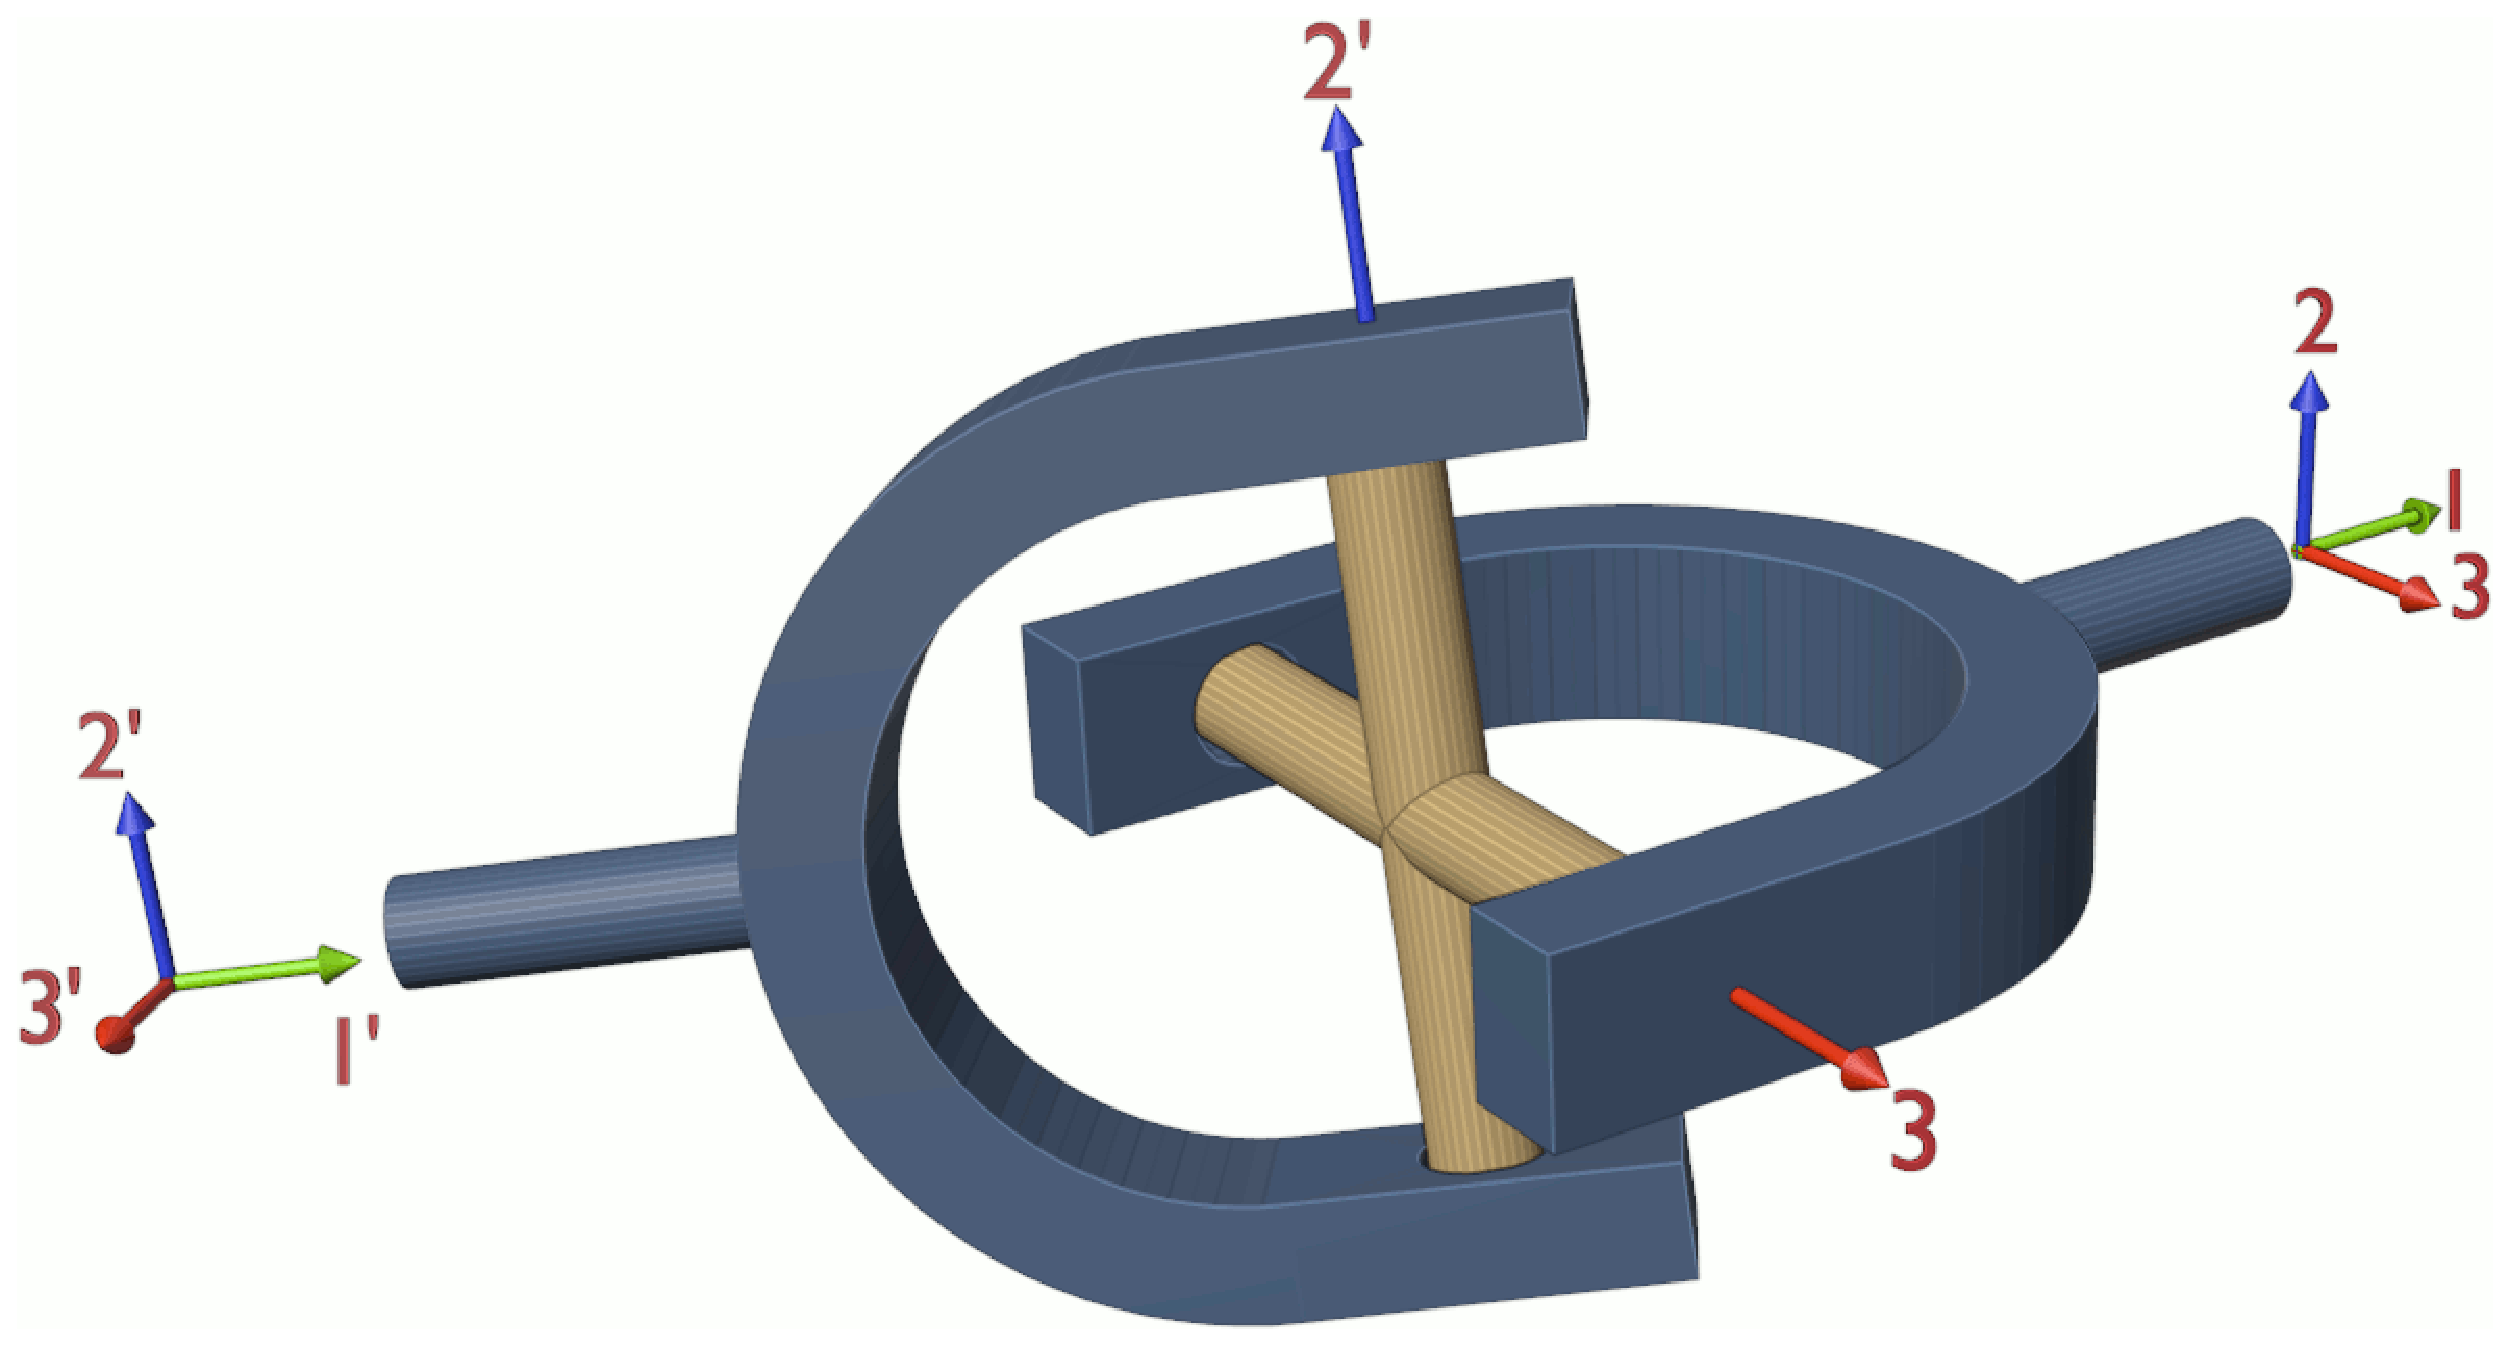
\includegraphics[width=.5\textwidth]{cardano}
\caption{Cardano hinge.}
\label{fig:el:joint:CARDANO}
\end{figure}
Note: this joint does not represent a constant velocity joint,
so, when a steady deflection between the two nodes is present,
a constant velocity about axis 1 of one node results in an oscillating
velocity about axis 1 for the other node.
The constant velocity joint is implemented by the \kw{gimbal joint}
(Section~\ref{sec:EL:JOINT:GIMBALROTATION}), which essentially consists
of a sequence of two
\hyperref{\kw{Cardano hinge}}{\kw{Cardano hinge} (see Section~}{)}{sec:EL:STRUCT:JOINT:CARDANO_HINGE}
joints with the hinges in reversed order, assembled
in a manner that the deflection is split half and half
between the two joints.

\subsection{Cardano pin}
\label{sec:EL:STRUCT:JOINT:CARDANO_PIN}
This joint implements a ``Cardano'' joint between a node and the ground.
The absolute position is also constrained.
See above for details about the formulation.
%\begin{verbatim}
\begin{Verbatim}[commandchars=\\\{\}]
    \bnt{joint_type} ::= \kw{Cardano pin}

    \bnt{joint_arglist} ::= 
        \bnt{node_label} ,
            \kw{position} , (\hty{Vec3}) \bnt{relative_offset}
            [ , \kw{orientation } , (\hty{OrientationMatrix}) \bnt{relative_orientation_matrix} ] ,
        \kw{position } , (\hty{Vec3}) \bnt{absolute_pin_position}
        [ , \kw{orientation} , (\hty{OrientationMatrix}) \bnt{absolute_pin_orientation_matrix} ]
\end{Verbatim}
%\end{verbatim}
\emph{Note: this is equivalent to a
\hyperref{\kw{Cardano hinge}}{\kw{Cardano hinge} (see Section~}{)}{sec:EL:STRUCT:JOINT:CARDANO_HINGE}
when one node is grounded.
}

\subsection{Cardano rotation}
\label{sec:EL:STRUCT:JOINT:CARDANO_ROTATION}
This joint implements a ``Cardano'' joint, which is made of a sequence
of two revolute hinges orthogonal to each other.
The relative position is not constrained.
See the \kw{Cardano hinge} for more details.
%\begin{verbatim}
\begin{Verbatim}[commandchars=\\\{\}]
    \bnt{joint_type} ::= \kw{Cardano rotation}

    \bnt{joint_arglist} ::= 
        \bnt{node_1_label}
            [ , \kw{orientation} , (\hty{OrientationMatrix}) \bnt{relative_orientation_matrix_1} ] ,
        \bnt{node_2_label}
            [ , \kw{orientation} , (\hty{OrientationMatrix}) \bnt{relative_orientation_matrix_2} ]
\end{Verbatim}
%\end{verbatim}

\emph{Note: this is equivalent to a
\hyperref{\kw{Cardano hinge}}{\kw{Cardano hinge} (see Section~}{)}{sec:EL:STRUCT:JOINT:CARDANO_HINGE}
without position constraint.
Or, in other words, a 
\hyperref{\kw{Cardano hinge}}{\kw{Cardano hinge} (see Section~}{)}{sec:EL:STRUCT:JOINT:CARDANO_HINGE}
is made of a \kw{Cardano rotation} on top of a 
\hyperref{\kw{spherical hinge}}{\kw{spherical hinge} (see Section~}{)}{sec:EL:STRUCT:JOINT:SPHERICAL_HINGE}.
}



\subsection{Clamp}
This joint grounds all 6 degrees of freedom of a node
in an arbitrary position and orientation that remains fixed.
%\begin{verbatim}
\begin{Verbatim}[commandchars=\\\{\}]
    \bnt{joint_type} ::= \kw{clamp}

    \bnt{joint_arglist} ::= \bnt{node_label} ,
        [ \kw{position} , ]
            \{ \kw{node} | (\hty{Vec3}) \bnt{absolute_position} \} ,
        [ \kw{orientation} , ]
            \{ \kw{node} | (\hty{OrientationMatrix}) \bnt{absolute_orientation_matrix} \}
\end{Verbatim}
%\end{verbatim}
The keyword \kw{node} forces the joint to use
the node's position and reference frame. Otherwise, they must be entered
in the usual way for these entities.
The default value for \kw{position} and \kw{orientation}
are the position and the orientation of the clamped node.

\subsubsection{Private Data}
The following data are available:
\begin{enumerate}
\item \kw{"Fx"} constraint reaction force in global direction 1
\item \kw{"Fy"} constraint reaction force in global direction 2
\item \kw{"Fz"} constraint reaction force in global direction 3
\item \kw{"Mx"} constraint reaction moment in local direction 1
\item \kw{"My"} constraint reaction moment in local direction 2
\item \kw{"Mz"} constraint reaction moment in local direction 3
\end{enumerate}




\subsection{Coincidence}
not implemented yet, use a
\hyperref{\kw{spherical hinge}}{\kw{spherical hinge} (see Section~}{)}{sec:EL:STRUCT:JOINT:SPHERICAL_HINGE}
and a \kw{prismatic} 
instead.




\subsection{Deformable Axial Joint}
\label{sec:EL:JOINT:DEFORMABLEAXIAL}
This joint implements a configuration (i.e.\ relative motion) dependent moment that is exchanged
between two nodes about an axis rigidly attached to the first node.
It is intended to be used in conjunction with another joint (for example a \kw{revolute hinge} or a \kw{total joint})
that constrains the relative rotation between the two nodes about the other axes,
although no check is in place.
%\begin{verbatim}
\begin{Verbatim}[commandchars=\\\{\}]
    \bnt{joint_type} ::= \kw{deformable axial joint}

    \bnt{joint_arglist} ::= 
        \bnt{node_1_label}
            [ , \kw{position} , (\hty{Vec3}) \bnt{relative_offset_1} ]
            [ , \kw{orientation} , (\hty{OrientationMatrix}) \bnt{relative_orientation_matrix_1} ] ,
        \bnt{node_2_label}
            [ , \kw{position} , (\hty{Vec3}) \bnt{relative_offset_2} ]
            [ , \kw{orientation} , (\hty{OrientationMatrix}) \bnt{relative_orientation_matrix_2} ] ,
        (\htybkw{ConstitutiveLaw}{1D}) \bnt{const_law}
\end{Verbatim}
%\end{verbatim}
The relative rotation is assumed to take place about axis 3 in the local reference frame of the joint,
as defined by \nt{relative\_orientation\_matrix\_1}.

\subsubsection{Private Data}
The following data are available:
\begin{enumerate}
\item \kw{"rz"} relative rotation about axis 3, used as strain in the constitutive law
\item \kw{"wz"} relative angular velocity about axis 3, used as strain rate in the constitutive law
\item \kw{"Mz"} moment about axis 3, output by the constitutive law
\end{enumerate}
In addition, the joint provides
access to any private data provided by the constitutive law.
They are accessed by prefixing the name of the data with the string
\kw{"constitutiveLaw."}; see the specific constitutive law
description of the available data in Section~\ref{sec:ConstitutiveLaw}.


\subsubsection{Hints}
When wrapped by a \kw{driven} element, the \kw{deformable axial joint}
honors the following hints:
\begin{itemize}
\item \kw{hinge\{1\}} the orientation with respect to node 1
of the reference used to compute the linear strain is reset
to the value resulting from the node 2 hinge orientation
and the node 1 orientation
\begin{displaymath}
	\tilde{\T{R}}_{1h} = \T{R}_1^T \T{R}_2 \tilde{\T{R}}_{2h}
\end{displaymath}
\item \kw{hinge\{2\}} the orientation with respect to node 2
of the reference used to compute the linear strain is reset
to the value resulting from the node 1 hinge orientation
and the node 2 orientation
\begin{displaymath}
	\tilde{\T{R}}_{2h} = \T{R}_2^T \T{R}_1 \tilde{\T{R}}_{1h}
\end{displaymath}
\item unrecognized hints are passed through to the constitutive law.
\end{itemize}

\subsubsection{Output}
In addition to the standard output, the \kw{deformable axial joint}
outputs:
\begin{itemize}
\item column 14: the relative rotation about axis 3
\end{itemize}
If the constitutive law is either viscous or viscoelastic:
\begin{itemize}
\item column 15: the relative angular velocity about axis 3
\end{itemize}
% Further optional columns contain any output from the constitutive law.



\subsection{Deformable displacement hinge}
Deprecated; use the 
\hyperref{\kw{deformable displacement joint}}
	{\kw{deformable displacement joint} (see Section~}{)}
	{sec:EL:JOINT:DEFORMABLEDISP}
instead.


\subsection{Deformable displacement joint}
\label{sec:EL:JOINT:DEFORMABLEDISP}
This joint implements a configuration dependent force that is exchanged
between two points associated with two nodes with an offset.
The force may depend, by way of a generic 3D constitutive law, 
on the relative position and velocity of the two points, 
expressed in the reference frame of node 1.

\noindent
The constitutive law is attached to the reference frame of node 1,
so the sequence of the connections may matter in case of anisotropic
constitutive laws, if the relative orientation of the two nodes
changes during the analysis.
%\begin{verbatim}
\begin{Verbatim}[commandchars=\\\{\}]
    \bnt{joint_type} ::= \kw{deformable displacement joint}

    \bnt{joint_arglist} ::= 
        \bnt{node_1_label} ,
            \kw{position} , (\hty{Vec3}) \bnt{relative_offset_1}
            [ , \kw{orientation} , (\hty{OrientationMatrix}) \bnt{relative_orientation_matrix_1} ] ,
        \bnt{node_2_label} ,
            \kw{position} , (\hty{Vec3}) \bnt{relative_offset_2}
            [ , \kw{orientation} , (\hty{OrientationMatrix}) \bnt{relative_orientation_matrix_2} ] ,
        (\htybkw{ConstitutiveLaw}{3D}) \bnt{const_law}
\end{Verbatim}
%\end{verbatim}

\noindent
Note: a variant of this element is under development,
which refers the material reference frame to an orientation 
that is intermediate between those of the two nodes.
See the
\hyperref{\kw{invariant deformable displacement joint}}
	{\kw{invariant deformable displacement joint} (Section~}{)}
	{sec:EL:JOINT:INVDEFORMABLEDISP}.



\subsubsection{Private Data}
The following data are available:
\begin{enumerate}
\item \kw{"dx"} relative displacement in node 1 local direction 1
\item \kw{"dy"} relative displacement in node 1 local direction 2
\item \kw{"dz"} relative displacement in node 1 local direction 3
\item \kw{"vx"} relative velocity in node 1 local direction 1
\item \kw{"vy"} relative velocity in node 1 local direction 2
\item \kw{"vz"} relative velocity in node 1 local direction 3
\item \kw{"Fx"} constraint reaction force in node 1 local direction 1
\item \kw{"Fy"} constraint reaction force in node 1 local direction 2
\item \kw{"Fz"} constraint reaction force in node 1 local direction 3
\end{enumerate}
In addition, the joint provides
access to any private data provided by the constitutive law.
They are accessed by prefixing the name of the data with the string
\kw{"constitutiveLaw."}; see the specific constitutive law
description of the available data in Section~\ref{sec:ConstitutiveLaw}.

\subsubsection{Hints}
When wrapped by a \kw{driven} element, the \kw{deformable displacement joint}
honors the following hints:
\begin{itemize}
\item \kw{hinge\{1\}} the orientation with respect to node 1
of the reference used to compute the linear strain is reset
to the value resulting from the node 2 hinge orientation
and the node 1 orientation
\begin{displaymath}
	\tilde{\T{R}}_{1h} = \T{R}_1^T \T{R}_2 \tilde{\T{R}}_{2h}
\end{displaymath}
\item \kw{hinge\{2\}} the orientation with respect to node 2
of the reference used to compute the linear strain is reset
to the value resulting from the node 1 hinge orientation
and the node 2 orientation
\begin{displaymath}
	\tilde{\T{R}}_{2h} = \T{R}_2^T \T{R}_1 \tilde{\T{R}}_{1h}
\end{displaymath}
\item \kw{offset\{1\}} the offset of the joint
with respect to node 1 is reset to the value resulting 
from the node 2 offset and the node 1 position
\begin{displaymath}
	\tilde{\T{f}}_1 = \T{R}_1^T \plbr{
		\T{x}_2
		+ \T{R}_2 \tilde{\T{f}}_2
		- \T{x}_1
	}
\end{displaymath}
\item \kw{offset\{2\}} the offset of the joint
with respect to node 2 is reset to the value resulting 
from the node 1 offset and the node 2 position
\begin{displaymath}
	\tilde{\T{f}}_2 = \T{R}_2^T \plbr{
		\T{x}_1
		+ \T{R}_1 \tilde{\T{f}}_1
		- \T{x}_2
	}
\end{displaymath}
\item unrecognized hints are passed through to the constitutive law.
\end{itemize}

\subsubsection{Output}
In addition to the standard output, the \kw{deformable displacement joint}
outputs:
\begin{itemize}
\item columns 14--16: the three components of the linear strain.
\end{itemize}
If the constitutive law is either viscous or viscoelastic:
\begin{itemize}
\item columns 17--19: the three components of the linear strain rate.
\end{itemize}



\subsection{Deformable Hinge}
\label{sec:EL:JOINT:DEFORMABLEHINGE}
This joint implements a configuration dependent moment that is exchanged
between two nodes.
The moment may depend, by way of a generic 3D constitutive law, 
on the relative orientation and angular velocity of the two nodes, 
expressed in the reference frame of node 1.

\noindent
The constitutive law is attached to the reference frame of node 1,
so the sequence of the connections may matter in case of anisotropic
constitutive laws, if the relative orientation of the two nodes
changes during the analysis.
%\begin{verbatim}
\begin{Verbatim}[commandchars=\\\{\}]
    \bnt{joint_type} ::= \kw{deformable hinge}

    \bnt{joint_arglist} ::= 
        \bnt{node_1_label}
            [ , \kw{position} , (\hty{Vec3}) \bnt{relative_position_1} ]
            [ , \kw{orientation} , (\hty{OrientationMatrix}) \bnt{relative_orientation_matrix_1} ] ,
        \bnt{node_2_label} 
            [ , \kw{position} , (\hty{Vec3}) \bnt{relative_position_2} ]
            [ , \kw{orientation} , (\hty{OrientationMatrix}) \bnt{relative_orientation_matrix_2} ] ,
        (\htybkw{ConstitutiveLaw}{3D}) \bnt{const_law}
        [ , \kw{orientation description} , \bnt{orientation_type} ]
\end{Verbatim}
%\end{verbatim}
\noindent
The \nt{orientation\_type} is defined
in Section~\ref{sec:CONTROLDATA:DEFAULTORIENTATION}.

Note: a variant of this element has been developed,
which refers the material reference frame to an orientation 
that is intermediate between those of the two nodes.
See the
\hyperref{\kw{invariant deformable hinge}}
	{\kw{invariant deformable hinge} (Section~}{)}
	{sec:EL:JOINT:INVDEFORMABLEHINGE}.

\noindent
Note: this joint only applies internal moments; no forces
and no constraints to displacements are applied.
Usually, it is best used in conjunction with a
\hyperref{\kw{spherical hinge}}{\kw{spherical hinge} (see Section~}{)}{sec:EL:STRUCT:JOINT:SPHERICAL_HINGE},
or any kind of joint that constrains the relative displacement
of the nodes as appropriate.

\subsubsection{Private Data}
The following data are available:
\begin{enumerate}
\item \kw{"rx"} relative rotation vector component in node 1 local direction 1
\item \kw{"ry"} relative rotation vector component in node 1 local direction 2
\item \kw{"rz"} relative rotation vector component in node 1 local direction 3
\item \kw{"wx"} relative angular velocity in node 1 local direction 1
\item \kw{"wy"} relative angular velocity in node 1 local direction 2
\item \kw{"wz"} relative angular velocity in node 1 local direction 3
\item \kw{"Mx"} constraint reaction moment in node 1 local direction 1
\item \kw{"My"} constraint reaction moment in node 1 local direction 2
\item \kw{"Mz"} constraint reaction moment in node 1 local direction 3
\end{enumerate}
In addition, the joint provides
access to the private data provided by the constitutive law.
They are accessed by prefixing the name of the data with the string
\kw{"constitutiveLaw."}; see the specific constitutive law
description of the available data in Section~\ref{sec:ConstitutiveLaw}.

\subsubsection{Hints}
When wrapped by a \kw{driven} element, the \kw{deformable hinge}
joint honors the following hints:
\begin{itemize}
\item \kw{hinge\{1\}} the orientation with respect to node 1
of the reference used to compute the angular strain is reset
to the value resulting from the node 2 hinge orientation
and the node 1 orientation
\begin{displaymath}
	\tilde{\T{R}}_{1h} = \T{R}_1^T \T{R}_2 \tilde{\T{R}}_{2h}
\end{displaymath}
\item \kw{hinge\{2\}} the orientation with respect to node 2
of the reference used to compute the angular strain is reset
to the value resulting from the node 1 hinge orientation
and the node 2 orientation
\begin{displaymath}
	\tilde{\T{R}}_{2h} = \T{R}_2^T \T{R}_1 \tilde{\T{R}}_{1h}
\end{displaymath}
\item unrecognized hints are passed through to the constitutive law.
\end{itemize}

\subsubsection{Output}
In addition to the standard output, the \kw{deformable joint}
outputs:
\begin{itemize}
\item columns 14--16 (or 14--22): the angular strain
in the selected orientation format (either three or nine columns,
according to the selected \kw{orientation description}, or to its 
\hyperref{default value)}{default value, see Section~}{)}{sec:CONTROLDATA:DEFAULTORIENTATION}.
\end{itemize}
If the constitutive law is either viscous or viscoelastic:
\begin{itemize}
\item columns 17--19 (or 23--25): the three components
of the angular strain rate.
\end{itemize}




\subsection{Deformable joint}
\label{sec:EL:JOINT:DEFORMABLEJOINT}
This joint implements a configuration dependent force and moment
that are exchanged by two points associated with two nodes with an offset.
The force the and moment may depend, by way of a generic 6D constitutive law,
on the relative position, orientation, velocity and angular velocity 
of the two points, expressed in the reference frame of node 1.
It may be thought of as a combination of a
\hyperref{\kw{deformable displacement joint}}
	{\kw{deformable displacement joint} (see Section~}{)}
	{sec:EL:JOINT:DEFORMABLEDISP}
and of a 
\hyperref{\kw{deformable hinge}}
	{\kw{deformable hinge} (see Section~}{)}
	{sec:EL:JOINT:DEFORMABLEHINGE};
a significant difference is that the \kw{deformable joint} uses a 6D
\hyperref{\kw{constitutive law}}
	{\kw{constitutive law} (see Section~}{)}
	{sec:ConstitutiveLaw},
so the force and the moment may both depend on the displacement
and on the orientation.

\noindent
The constitutive law is attached to the reference frame of node 1,
so the sequence of the connections may matter in case of anisotropic
constitutive laws, if the relative orientation of the two nodes
changes during the analysis.

\noindent
This element may add a considerable overhead because of the computation
of the cross-coupling effects between the forces and moments and the
relative positions and orientations; if the constitutive law does not couple
relative displacements and orientations, a better choice consists 
in combining a \kw{deformable hinge} and a \kw{deformable displacement joint}.
%\begin{verbatim}
\begin{Verbatim}[commandchars=\\\{\}]
    \bnt{joint_type} ::= \kw{deformable joint}

    \bnt{joint_arglist} ::= 
        \bnt{node_1_label} ,
            \kw{position} , (\hty{Vec3}) \bnt{relative_offset_1}
            [ , \kw{orientation} ,(\hty{OrientationMatrix}) \bnt{relative_orientation_matrix_1} ] ,
        \bnt{node_2_label} ,
            \kw{position} , (\hty{Vec3}) \bnt{relative_offset_2}
            [ , \kw{orientation} , (\hty{OrientationMatrix}) \bnt{relative_orientation_matrix_2} ] ,
        (\htybkw{ConstitutiveLaw}{6D}) \bnt{const_law}
        [ , \kw{orientation description} , \bnt{orientation_type} ]
\end{Verbatim}
%\end{verbatim}
The \nt{orientation\_type} is defined
in Section~\ref{sec:CONTROLDATA:DEFAULTORIENTATION}.

\subsubsection{Private Data}
The following data are available:
\begin{enumerate}
\item \kw{"dx"} relative displacement in node 1 local direction 1
\item \kw{"dy"} relative displacement in node 1 local direction 2
\item \kw{"dz"} relative displacement in node 1 local direction 3
\item \kw{"rx"} relative rotation vector component in node 1 local direction 1
\item \kw{"ry"} relative rotation vector component in node 1 local direction 2
\item \kw{"rz"} relative rotation vector component in node 1 local direction 3
\item \kw{"vx"} relative velocity in node 1 local direction 1
\item \kw{"vy"} relative velocity in node 1 local direction 2
\item \kw{"vz"} relative velocity in node 1 local direction 3
\item \kw{"wx"} relative angular velocity in node 1 local direction 1
\item \kw{"wy"} relative angular velocity in node 1 local direction 2
\item \kw{"wz"} relative angular velocity in node 1 local direction 3
\item \kw{"Fx"} constraint reaction force in node 1 local direction 1
\item \kw{"Fy"} constraint reaction force in node 1 local direction 2
\item \kw{"Fz"} constraint reaction force in node 1 local direction 3
\item \kw{"Mx"} constraint reaction moment in node 1 local direction 1
\item \kw{"My"} constraint reaction moment in node 1 local direction 2
\item \kw{"Mz"} constraint reaction moment in node 1 local direction 3
\end{enumerate}
In addition, the joint provides
access to the private data provided by the constitutive law.
They are accessed by prefixing the name of the data with the string
\kw{"constitutiveLaw."}; see the specific constitutive law
description of the available data in Section~\ref{sec:ConstitutiveLaw}.

\subsubsection{Hints}
When wrapped by a \kw{driven} element, the \kw{deformable joint}
honors the same hints of the \kw{deformable displacement joint}.

\subsubsection{Output}
In addition to the standard output, the \kw{deformable joint}
outputs:
\begin{itemize}
\item columns 14--16: the three components of the linear strain;
\item columns 17--19 (or 17--25): the angular strain
in the selected orientation format (either three or nine columns,
according to the selected \kw{orientation description}, or to its 
\hyperref{default value)}{default value, see Section~}{)}{sec:CONTROLDATA:DEFAULTORIENTATION}.
\end{itemize}
If the constitutive law is either viscous or viscoelastic:
\begin{itemize}
\item columns 20--22 (or 26--28): the three components
of the linear strain rate;
\item columns 23--25 (or 29--31): the three components
of the angular strain rate.
\end{itemize}




\subsection{Distance}
This joint forces the distance between two points,
each relative to a node, to assume the value indicated by the drive.
If no offset is given, the points are coincident with the node themselves.
%\begin{verbatim}
\begin{Verbatim}[commandchars=\\\{\}]
    \bnt{joint_type} ::= \kw{distance}

    \bnt{joint_arglist} ::=
        \bnt{node_1_label} , 
        [ \kw{position} , \bnt{relative_offset_1} , ]
        \bnt{node_2_label} ,
        [ \kw{position} , \bnt{relative_offset_2} , ]
        \{ (\hty{DriveCaller}) \bnt{distance} | \kw{from nodes} \}
\end{Verbatim}
%\end{verbatim}
The \nt{relative\_offset\_*} are the distances of each end
of the joint from the relative nodes in the node reference frame.
The \kw{distance} and the \kw{distance with offset} joints
do not allow null distance.

Note: in case the keyword \kw{from nodes} is used, a constant drive
caller is automatically instantiated for the \kw{distance}. 
Its value is computed from the initial positions of the nodes;
if any of the offsets is specified, the distance between the offset points is actually considered. 



\subsubsection{Current}
When parsing the drive caller, the following values are made available
through the \kw{model::current} interface:
\begin{itemize}
\item
\kw{"L"}: 
the distance between the points connected by the joint,
as it would be computed when \kw{from nodes} is used.
\end{itemize}
For example, to smoothly change the distance from the initial value to a desired value:
\begin{verbatim}
    set: const integer DISTANCE = 99;
    set: const integer NODE1 = 1;
    set: const integer NODE2 = 2;
    set: const real DESIRED_DISTANCE = .33;
    # ...
    joint: DISTANCE, distance,
        NODE1, position, null,
        NODE2, position, null,
        cosine, 0., pi/.5,
            (DESIRED_DISTANCE - model::current("L"))/2,  # half (desired - initial)
            half,
            model::current("L");                         # start from initial
\end{verbatim}



\subsubsection{Output}
The extra output is:
\begin{itemize}
    \item the three components of unit vector representing the imposed 
      distance direction in the global frame
    \item the norm of the imposed distance
\end{itemize}

\subsubsection{Private Data}
The following data are available:
\begin{enumerate}
\item \kw{"d"} enforced distance
\end{enumerate}

\subsubsection{Hints}
When wrapped by a \kw{driven} element, the following hints are honored:
\begin{itemize}
\item unrecognized hints are passed through to the distance drive.
\end{itemize}



\subsection{Distance with offset}
This element has been deprecated in favor of the \kw{distance}
joint element, which now supports offsets.
It may be dropped in future releases.

\subsubsection{Private Data}
See the \kw{distance} joint element.



\subsection{Drive displacement}
\label{sec:EL:JOINT:DRIVEDISPLACEMENT}
This joint imposes the relative position between two points 
optionally offset from two structural nodes,
in the form of a vector that expresses the direction of the displacement
in the reference frame of node 1, whose amplitude is defined by a drive.
%\begin{verbatim}
\begin{Verbatim}[commandchars=\\\{\}]
    \bnt{joint_type} ::= \kw{drive displacement}

    \bnt{joint_arglist} ::= 
        \bnt{node_1_label} , (\hty{Vec3}) \bnt{offset_1} ,
        \bnt{node_2_label} , (\hty{Vec3}) \bnt{offset_2} ,
        (\htybty{TplDriveCaller}{Vec3}) \bnt{relative_position}
\end{Verbatim}
%\end{verbatim}
This element is superseded by the
\hyperref{\kw{total joint}}{\kw{total joint}, see Section~}{}{sec:EL:STRUCT:JOINT:TOTAL_JOINT}.

\subsubsection{Private Data}
The following data are available:
\begin{enumerate}
\item \kw{"dx"} imposed displacement component along node 1 axis 1
\item \kw{"dy"} imposed displacement component along node 1 axis 2
\item \kw{"dz"} imposed displacement component along node 1 axis 3
\item \kw{"fx"} reaction force component along node 1 axis 1
\item \kw{"fy"} reaction force component along node 1 axis 2
\item \kw{"fz"} reaction force component along node 1 axis 3
\end{enumerate}

\subsubsection{Hints}
When wrapped by a \kw{driven} element, the following hints are honored:
\begin{itemize}
\item \kw{offset\{1\}} the offset of the joint
with respect to node 1 is reset by pointing 
to the drive displacement point;
\item \kw{offset\{2\}} the offset of the joint
with respect to node 2 is reset by pointing 
to the drive displacement point;
\item unrecognized hints are passed through to the \htybty{TplDriveCaller}{Vec3}.
\end{itemize}



\subsection{Drive displacement pin}
\label{sec:EL:JOINT:DRIVEDISPLACEMENTPIN}
This joint imposes the absolute position of a point optionally offset
from a structural node, in the form of a vector that expresses 
the direction of the displacement in the absolute reference frame,
whose amplitude is defined by a drive.
%\begin{verbatim}
\begin{Verbatim}[commandchars=\\\{\}]
    \bnt{joint_type} ::= \kw{drive displacement pin}

    \bnt{joint_arglist} ::= 
        \bnt{node_label} , (\hty{Vec3}) \bnt{node_offset} ,
        (\hty{Vec3}) \bnt{offset} ,
        (\htybty{TplDriveCaller}{Vec3}) \bnt{position}
\end{Verbatim}
%\end{verbatim}
This element is superseded by the
\hyperref{\kw{total pin joint}}{\kw{total pin joint}, see Section~}{}{sec:EL:STRUCT:JOINT:TOTAL_PIN_JOINT}.

\subsubsection{Private Data}
The following data are available:
\begin{enumerate}
\item \kw{"dx"} imposed displacement component along absolute axis 1
\item \kw{"dy"} imposed displacement component along absolute axis 2
\item \kw{"dz"} imposed displacement component along absolute axis 3
\item \kw{"fx"} reaction force component along absolute axis 1
\item \kw{"fy"} reaction force component along absolute axis 2
\item \kw{"fz"} reaction force component along absolute axis 3
\end{enumerate}

\subsubsection{Hints}
When wrapped by a \kw{driven} element, the following hints are honored:
\begin{itemize}
\item \kw{offset\{1\}} the offset of the joint
with respect to the node is reset by pointing 
to the driven displacement point;
\item \kw{offset\{0\}} the offset of the joint
with respect to the absolute reference frame is reset by pointing
to the driven displacement point;
\item unrecognized hints are passed through to the \htybty{TplDriveCaller}{Vec3}.
\end{itemize}



\subsection{Drive hinge}
\label{sec:EL:JOINT:DRIVEHINGE}
This joint imposes the relative orientation between two nodes,
in the form of a rotation about an axis whose amplitude is defined
by a drive.
%\begin{verbatim}
\begin{Verbatim}[commandchars=\\\{\}]
    \bnt{joint_type} ::= \kw{drive hinge}

    \bnt{joint_arglist} ::= 
        \bnt{node_1_label}
            [ , \kw{orientation} , (\hty{OrientationMatrix}) \bnt{relative_orientation_matrix_1} ] ,
        \bnt{node_2_label}
            [ , \kw{orientation} , (\hty{OrientationMatrix}) \bnt{relative_orientation_matrix_2} ] ,
        (\htybty{TplDriveCaller}{Vec3}) \bnt{hinge_orientation}
\end{Verbatim}
%\end{verbatim}
This element is superseded by the
\hyperref{\kw{total joint}}{\kw{total joint}, see Section~}{}{sec:EL:STRUCT:JOINT:TOTAL_JOINT}.

Note: this element is experimental; now it is more reliable, 
but it is limited to $\nrbr{\nt{hinge\_orientation}} < \pi$.

\subsubsection{Private Data}
The following data are available:
\begin{enumerate}
\item \kw{"rx"} imposed relative rotation about node 1 hinge axis 1
\item \kw{"ry"} imposed relative rotation about node 1 hinge axis 2
\item \kw{"rz"} imposed relative rotation about node 1 hinge axis 3
\item \kw{"Mx"} reaction moment about node 1 hinge axis 1
\item \kw{"My"} reaction moment about node 1 hinge axis 2
\item \kw{"Mz"} reaction moment about node 1 hinge axis 3
\end{enumerate}
When wrapped by a \kw{driven} element, the following hints are honored:
\begin{itemize}
\item \kw{hinge\{1\}} the orientation with respect to node 1
of the reference in which the enforced orientation is expressed is reset;
\item \kw{hinge\{2\}} the orientation with respect to node 2
of the reference in which the enforced orientation is expressed is reset;
\item unrecognized hints are passed through to the \htybty{TplDriveCaller}{Vec3}.
\end{itemize}

\subsection{Gimbal hinge}
This joint has not been implemented yet; use a \kw{gimbal rotation}
and a
\hyperref{\kw{spherical hinge}}{\kw{spherical hinge} (see Section~}{)}{sec:EL:STRUCT:JOINT:SPHERICAL_HINGE}
to emulate.

\subsection{Gimbal rotation}\label{sec:EL:JOINT:GIMBALROTATION}
A homokinetic joint without position constraints;
this joint, in conjunction with a
\hyperref{\kw{spherical hinge}}{\kw{spherical hinge} (see Section~}{)}{sec:EL:STRUCT:JOINT:SPHERICAL_HINGE}
joint, should be used to implement an ideal tiltrotor gimbal
instead of a
\hyperref{\kw{Cardano rotation}}{\kw{Cardano rotation} (see Section~}{)}{sec:EL:STRUCT:JOINT:CARDANO_ROTATION}.
See the technical manual and \cite{GIMBAL-2008} for details.
It is equivalent to a series of two Cardano's joints
(the \hyperref{\kw{Cardano hinge}}{\kw{Cardano hinge}, see Section~}{}{sec:EL:STRUCT:JOINT:CARDANO_HINGE})
rotated 90 degrees apart, each accounting for half the relative rotation
between axis 3 of each side of the joint.
%\begin{verbatim}
\begin{Verbatim}[commandchars=\\\{\}]
    \bnt{joint_type} ::= \kw{gimbal rotation}

    \bnt{joint_arglist} ::= 
        \bnt{node_1_label}
        [ , \kw{orientation} , (\hty{OrientationMatrix}) \bnt{relative_orientation_matrix_1} ] ,
        \bnt{node_2_label}
        [ , \kw{orientation} , (\hty{OrientationMatrix}) \bnt{relative_orientation_matrix_2} ]
        [ , \kw{orientation description} , \bnt{orientation_type} ]
\end{Verbatim}
%\end{verbatim}
The \nt{orientation\_type} is defined
in Section~\ref{sec:CONTROLDATA:DEFAULTORIENTATION}.

This joint allows nodes 1 and 2 to rotate about relative axes 1 and 2.

\subsubsection{Output}
The \kw{gimbal rotation} joint outputs the three components
of the reaction couple in the local frame (that of node 1) 
and in the global frame.

The extra columns 14 and 15 contain the angles $\vartheta$ and $\varphi$.
The extra columns from 16 on contain the relative rotation
between nodes 1 and 2, in the format determined either by an explicit
selection of the orientation description, or by the default
orientation description defined by the 
\hyperref{\kw{default orientation} keyword}{\kw{default orientation} keyword (see Section~}{)}{sec:CONTROLDATA:DEFAULTORIENTATION}.

The three components of the reaction couple in the local frame, 
and the angles $\vartheta$ and $\varphi$ are also available
as private data of the element under the names \kw{lambda[\bnt{i}]},
with \nt{i} = 1, 2, 3, \kw{theta} and \kw{phi}.
For a description of the formulation and of the angles describe above,
see the Technical Manual.

\subsubsection{Private Data}
The following data are available:
\begin{enumerate}
\item \kw{"lambda[1]"} constraint reaction moment about node 1 local axis 1
\item \kw{"lambda[2]"} constraint reaction moment about node 1 local axis 2
\item \kw{"lambda[3]"} constraint reaction moment about node 1 local axis 3
\item \kw{"theta"} relative angle $\vartheta$
\item \kw{"phi"} relative angle $\varphi$
\end{enumerate}



\subsection{Imposed displacement}
\label{sec:EL:JOINT:IMPOSEDDISPLACEMENT}
This joint imposes the relative position between two points,
optionally offset from two structural nodes,
along a given direction that is rigidly attached to the first node.
The amplitude of the displacement is defined by a drive.
%\begin{verbatim}
\begin{Verbatim}[commandchars=\\\{\}]
    \bnt{joint_type} ::= \kw{imposed displacement}

    \bnt{joint_arglist} ::= 
        \bnt{node_1_label} , (\hty{Vec3}) \bnt{offset_1} ,
        \bnt{node_2_label} , (\hty{Vec3}) \bnt{offset_2} ,
        (\hty{Vec3}) \bnt{direction} ,
        (\hty{DriveCaller}) \bnt{relative_position}
\end{Verbatim}
%\end{verbatim}
This element is superseded by the
\hyperref{\kw{total joint}}{\kw{total joint}, see Section~}{}{sec:EL:STRUCT:JOINT:TOTAL_JOINT}.

\subsubsection{Private Data}
The following data are available:
\begin{enumerate}
\item \kw{"d"} imposed displacement along \nt{direction},
in node 1 reference frame;
\item \kw{"f"} reaction force along \nt{direction},
in node 1 reference frame.
\end{enumerate}

\subsubsection{Hints}
When wrapped by a \kw{driven} element, the following hints are honored:
\begin{itemize}
\item \kw{offset\{1\}} the offset of the joint
with respect to node 1 is reset by pointing exactly
to the imposed displacement point;
\item \kw{offset\{2\}} the offset of the joint
with respect to node 2 is reset by pointing exactly
to the imposed displacement point;
\item unrecognized hints are passed through to the drive.
\end{itemize}



\subsection{Imposed displacement pin}
\label{sec:EL:JOINT:IMPOSEDDISPLACEMENTPIN}
This joint imposes the absolute displacement of a point optionally offset
from a structural node, along a direction defined
in the absolute reference frame.
The amplitude of the displacement is defined by a drive.
%\begin{verbatim}
\begin{Verbatim}[commandchars=\\\{\}]
    \bnt{joint_type} ::= \kw{imposed displacement pin}

    \bnt{joint_arglist} ::= 
        \bnt{node_label} , (\hty{Vec3}) \bnt{node_offset} ,
        (\hty{Vec3}) \bnt{offset} ,
        (\hty{Vec3}) \bnt{direction} ,
        (\hty{DriveCaller}) \bnt{position}
\end{Verbatim}
%\end{verbatim}
This element is superseded by the
\hyperref{\kw{total pin joint}}{\kw{total pin joint}, see Section~}{}{sec:EL:STRUCT:JOINT:TOTAL_PIN_JOINT}.

\subsubsection{Private Data}
The following data are available:
\begin{enumerate}
\item \kw{"x"} imposed displacement along \nt{direction},
in the absolute reference frame;
\item \kw{"f"} reaction force along \nt{direction},
in the absolute reference frame.
\end{enumerate}

\subsubsection{Hints}
When wrapped by a \kw{driven} element, the following hints are honored:
\begin{itemize}
\item \kw{offset\{1\}} the offset of the joint
with respect to the node is reset by pointing exactly
to the imposed displacement point;
\item \kw{offset\{0\}} the offset of the joint
with respect to the absolute reference frame is reset by pointing exactly
to the imposed displacement point;
\item unrecognized hints are passed through to the drive.
\end{itemize}




\subsection{In line}
This joint forces a point relative to the second node to move 
along a line attached to the first node.
%\begin{verbatim}
\begin{Verbatim}[commandchars=\\\{\}]
    \bnt{joint_type} ::= \kw{in line}

    \bnt{joint_arglist} ::= 
        \bnt{node_1_label} , 
            [ \kw{position} , ] (\hty{Vec3}) \bnt{relative_line_position} ,
            [ \kw{orientation} , ] (\hty{OrientationMatrix}) \bnt{relative_orientation} ,
        \bnt{node_2_label}
            [ , \kw{offset} , (\hty{Vec3}) \bnt{relative_offset} ]
	[ , \kw{friction} ,
            [ \kw{preload} , \bnt{const_value} , ]
            \bnt{friction_model} , 
            \bnt{shape_function} ]
\end{Verbatim}
%\end{verbatim}
A point, optionally offset by \nt{relative\_offset} from the position
of node \nt{node\_2\_label}, slides along a line that passes through a point 
that is rigidly offset by \nt{relative\_line\_position}
from the position of \nt{node\_1\_label}, and is directed as direction 3 
of \nt{relative\_orientation}.
Note that the \kw{friction} keyword can currently only be used with the \kw{in line} joint without \kw{offset}.
The joint is shown in Figure~\ref{fig:el:joint:INLINE} where the origin and orientation of \nt{node\_1} are given by axis 1$^\prime$, 2$^\prime$, 3$^\prime$ and \nt{relative\_line\_position} and \nt{relative\_orientation} are the transformations that yield axis 1$^\prime_0$, 2$^\prime_0$, 3$^\prime_0$ when applied to its coordinate axis. The origin and orientation of \nt{node\_2} are given by axis 1, 2, 3 and axis 1$_0$, 2$_0$, 3$_0$ is the result of applying the \nt{relative\_offset} translation to its coordinate axis.
\begin{figure}
\centering

\includegraphics[width=.5\textwidth]{inline}
\caption{Inline joint.}
\label{fig:el:joint:INLINE}
\end{figure}
\subsubsection{Output}
The output occurs in the \texttt{.jnt} file, according to default joint output
for the first 13 columns; if friction is present the additional output is:
\begin{itemize}
\item column 14: the friction force along the line of the joint (applied in negative and positive directions for nodes 1 and 2, respectively);
\item column 15: the friction coefficient;
\item column 16: the relative sliding velocity;
\item column 17: the relative sliding displacement.
\end{itemize}



\subsection{In plane}
This joint forces a point relative to the second node to move 
in a plane attached to the first node.
%\begin{verbatim}
\begin{Verbatim}[commandchars=\\\{\}]
    \bnt{joint_type} ::= \kw{in plane}

    \bnt{joint_arglist} ::= 
        \bnt{node_1_label} , 
        [ \kw{position} , ] (\hty{Vec3}) \bnt{relative_plane_position} ,
        ((\ty{Unit})\hty{Vec3}) \bnt{relative_normal_direction} ,
        \bnt{node_2_label}
        [ , \kw{offset} , (\hty{Vec3}) \bnt{relative_offset} ]
\end{Verbatim}
%\end{verbatim}
A point, optionally offset by \nt{relative\_offset} from the position
of node \nt{node\_2\_label}, slides on a plane that passes through a point 
that is rigidly offset by \nt{relative\_plane\_position}
from the position of \nt{node\_1\_label}, and is perpendicular to 
\nt{relative\_normal\_direction}.
The vector \nt{relative\_normal\_direction} is internally normalized to unity.



\subsection{Invariant deformable displacement joint}\label{sec:EL:JOINT:INVDEFORMABLEDISP}
Under development; right now, use the
\hyperref{\kw{deformable displacement joint}}
	{\kw{deformable displacement joint} (see Section~}{)}
	{sec:EL:JOINT:DEFORMABLEDISP}
instead.



\subsection{Invariant deformable hinge}\label{sec:EL:JOINT:INVDEFORMABLEHINGE}
This (experimental) element is a variant of the
\hyperref{\kw{deformable hinge}}
	{\kw{deformable hinge} (see Section~}{)}
	{sec:EL:JOINT:DEFORMABLEHINGE};
refer to that joint for the input syntax.

\noindent
The \emph{invariant} form of the \kw{deformable hinge} joint 
refers the constitutive law to an orientation that is intermediate 
between those of the nodes it connects.
As a result, the moment exchanged between the two nodes
is invariant to the sequence of definition of the nodes
when anisotropic constitutive laws are used.
It is worth stressing that determining the constitutive law for this
element may be tricky, since usual measurement approaches
directly measure forces and moments in a reference frame
that is attached to one of the two ends of the component,
so in practical cases it might be more appropriate to use the
\emph{variant} form of the joint, and consistently referring
the constitutive law to the same end used to measure
the mechanical properties of the component.

%%% FIXME: the residual (and the tecman) is available,
%%% but needs work to split it out of the DeformableHinge,
%%% define it as a separate element, and implement
%%% the Jacobian matrix contribution


\begin{comment}
\subsection{Kinematic}
This joint will eventually evolve into a connection with external programs
that impose the entire motion of a node; at present, you can use it
by directly writing code in files \verb;mbdyn/struct/kin.cc; and
\verb;mbdyn/struct/kin.h; that implement the motion you wish to impose.
%\begin{verbatim}
\begin{Verbatim}[commandchars=\\\{\}]
    \bnt{joint_type} ::= \kw{kinematic}

    \bnt{joint_arglist} ::= 
        \bnt{node_1_label} ,
        (\hty{DriveCaller}) \bnt{input}
\end{Verbatim}
%\end{verbatim}
This element is superseded by the
\hyperref{\kw{total pin joint}}{\kw{total pin joint}, see Section~}{}{sec:EL:STRUCT:JOINT:TOTAL_PIN_JOINT}.

Note: this element is eXperimental.
\end{comment}

\subsection{Linear acceleration}
This joint imposes the absolute linear acceleration of a node
along a given axis.
%\begin{verbatim}
\begin{Verbatim}[commandchars=\\\{\}]
    \bnt{joint_type} ::= \kw{linear acceleration}

    \bnt{joint_arglist} ::=
        \bnt{node_label} ,
        ((\ty{Unit})\hty{Vec3}) \bnt{relative_direction} , 
        (\hty{DriveCaller}) \bnt{acceleration}
\end{Verbatim}
%\end{verbatim}
The axis is \nt{relative\_direction}; it is internally normalized to unity.

\subsubsection{Private Data}
The following data are available:
\begin{enumerate}
\item \kw{"F"} constraint reaction force along joint direction
\item \kw{"a"} imposed acceleration along joint direction
\end{enumerate}

\subsection{Linear velocity}
This joint imposes the absolute linear velocity of a node
along a given axis.
%\begin{verbatim}
\begin{Verbatim}[commandchars=\\\{\}]
    \bnt{joint_type} ::= \kw{linear velocity}

    \bnt{joint_arglist} ::=
        \bnt{node_label} ,
        ((\ty{Unit})\hty{Vec3}) \bnt{relative_direction} , 
        (\hty{DriveCaller}) \bnt{velocity}
\end{Verbatim}
%\end{verbatim}
The axis is \nt{relative\_direction}; it is internally normalized to unity.

\subsubsection{Private Data}
The following data are available:
\begin{enumerate}
\item \kw{"v"} imposed velocity along joint direction
\end{enumerate}



\subsection{Modal}\label{sec:EL:STRUCT:JOINT:MODAL}
\emph{
Original implementation: Felice Felippone; \\
Initial review: Giuseppe Quaranta; \\
Current review: Pierangelo Masarati.}

This joint implements a Component Mode Synthesis (CMS) deformable body.
Its interface with the multibody domain is represented by clamps
that constrain the multibody interface nodes to the position
and orientation of the corresponding FEM nodes.
%\begin{verbatim}
\begin{Verbatim}[commandchars=\\\{\}]
    \bnt{joint_type} ::= \kw{modal}

    \bnt{joint_arglist} ::=
        \{ \bnt{reference_modal_node} | \kw{clamped}
            [ , \kw{position} , (\hty{Vec3}) \bnt{absolute_position} ]
            [ , \kw{orientation} , (\hty{OrientationMatrix}) \bnt{absolute_orientation} ] \} ,
        \bnt{mode_number} ,
        [ \kw{list} , \bnt{mode} [ , ... ] , ]
        [ \kw{initial value} ,
            \{ \kw{mode} , \bnt{j} , \bnt{q_j} , \bnt{qP_j} [ , ... ]  # 1 <= \nt{j} <= \nt{mode_number}
                | \bnt{q_1} , \bnt{qP_1} [ , ... ] \} , ]
        \{ \bnt{FEM_node_number} | \kw{from file} \} ,
        [ \{ \kw{no damping}
            | \kw{damping from file}
            | \kw{rayleigh damping} , \bnt{mass_damping_coef} , \bnt{stiffness_damping_coef}
            | \kw{single factor damping} , \bnt{damping_factor}
            | \kw{diag damping} ,
                \{ \kw{all} , \bnt{damping_factor} [ , ...]
                | \bnt{num_damped_modes} , \bnt{mode_damping} [ , ... ] \} \} , ]
        " \bnt{FEM_data_file} " ,
        [ [ \{ \kw{mass} | \kw{damping} | \kw{stiffness} \} ] \kw{threshold} , \bnt{threshold} , ]
        [ \{ \kw{create binary} | \kw{use binary} | \kw{update binary} \}
            [ , ... ] , ]
        [ \kw{echo} , " \bnt{echo_FEM_data_file} " [ , \kw{precision} , \bnt{precision_digits} ] , ]
        [ \kw{use invariant 9} , ]
        [ \{ \kw{origin node} , \bnt{origin_node} | \kw{origin position} , (\hty{Vec3}) \bnt{pos} \} , ]
	\bnt{interface_nodes_number} ,
	    [ \kw{output} , \{ \kw{yes} | \kw{no} | (\ty{bool})\bnt{output_flag_for_all_interfaces} \} , ]
            [ \kw{interface tolerance} , \bnt{interface_tolerance} , ]
	    \bnt{interface_node} [ , ... ]

    \bnt{mode_damping} ::= \bnt{mode_index} , \bnt{mode_damping_factor}

    \bnt{interface_node} ::=
        \{ " \bnt{FEM_node_label} "
                | (\ty{integer}) \bnt{FEM_node_label}
                | \kw{find closest} [ , \kw{interface tolerance} , \bnt{interface_tolerance} ] \} ,
            \bnt{multibody_label} , (\hty{Vec3}) \bnt{offset_of_FEM_node}
	        [ , \kw{output} , \{ \kw{yes} | \kw{no} | (\ty{bool})\bnt{output_flag_for_this_interface} \} ]
\end{Verbatim}
%\end{verbatim}
The \nt{reference\_modal\_node} is a special dynamic structural node 
that is required to handle the rigid body motion of the modal joint.
Its input is completely analogous to that of the \kw{dynamic} structural
nodes, see Section~\ref{sec:NODE:STRUCTURAL}, only the keyword \kw{dynamic} 
must be replaced by \kw{modal}.

If no rigid body dynamics is required, e.g.\ if the modal element
is clamped, the \kw{clamped} option can be used, which allows
to set the optional \nt{absolute\_position}
and \nt{absolute\_orientation}.
The former is the location, in the multibody
global reference system, of the origin of the FEM reference system.
The latter is the orientation,
in the multibody global reference frame,
of the FEM reference system.
They default to zero and identity, which means
that the global multibody reference frame
and the FEM reference system are coincident.

The mode count in \nt{mode\_number} is not required to match
the number of modes listed in the FEM data file; if a lower number
is given, only the first \nt{mode\_number} modes are used;
moreover, a list of active modes can be given, to use non-consecutive
modes; e.g., to use modes 1, 2, 3 and 6 out of a set of 10 modes
defined in the FEM data file, write
\begin{verbatim}
    ...,
    4,                        # number of active modes
        list, 1, 2, 3, 6,     # list of active modes
    ...
\end{verbatim}

By default, the origin of the FEM grid is placed either in the position
of the modal node, with its orientation, or in the absolute position 
and orientation in case the modal element is clamped, 
unless one of the mutually exclusive \kw{origin node} 
and \kw{origin position} optional keywords is used.
The \kw{origin node} keyword defines what FEM node corresponds 
to the \kw{modal} node in the multibody domain,
or what FEM node corresponds to the optional absolute position 
and orientation in case of a clamped modal element.
The \kw{origin position} keyword defines where, in the FEM model
reference frame, the \kw{modal} node is placed, or the location
that corresponds to the optional absolute position and orientation
in case of a clamped modal element.

Note that having the \kw{modal} node coincident with a FEM node
does not guarantee that the two remain coincident during the analysis.
This is only true if the modal shape displacements and rotations of the FEM node
are identically zero (i.e.\ in case of \emph{attached modes}).
Otherwise, the FEM node initially coincident with the \kw{modal} node
departs from it as long as the modal coordinates (the mode shape multipliers) are non-zero.

The FEM labels can be strings made of any character,
provided they do not contain blanks.
The strings must be enclosed in double quotes.
For legacy reasons, a label not enclosed in double quotes
is accepted, provided it is an integer.

The list of matchings between FEM and multibody nodes needs
special care.
The \nt{offset\_of\_FEM\_node} field contains the distance
of the FEM node from the respective multibody node; by default,
this is expressed in the reference frame of the multibody node.

Each FEM node which needs to be exposed in the multibody domain must be 
in the list of ``interface nodes'', where it is paired with the corresponding multibody node.
It is suggested that the latter be defined as a \kw{static} node, unless additional mass needs to be attached to it in the multibody domain,
since the multibody node will be ``clamped'' to the \kw{modal} joint.
Each \nt{interface\_node} can be defined using its \nt{FEM\_node\_label} (the FEM node label, either a string or an integer),
or using the special keyword \kw{find closest}.
In the latter case, the FEM node which is closest to the multibody node (including the offset)
is looked up.

If any of \kw{mass threshold}, \kw{damping threshold}, \kw{stiffness threshold} are given,
matrix elements whose absolute value is lower than the threshold
are discarded from the mass, damping and stiffness matrices, respectively.
The keyword \kw{threshold} is a catchall for all,
meaning that the same threshold is used for all matrices.

The \nt{FEM\_data\_file} can be generated by NASTRAN, 
following the procedure illustrated
in Appendix~\ref{sec:APP:EL:STRUCT:JOINT:MODAL:NASTRAN}.

It is strongly recommended that constrained modal analysis
be used for otherwise free bodies, with the statically 
determined constraint consisting of clamping the FEM node 
that will coincide with the node indicated as \nt{reference\_modal\_node},
and using the \kw{origin node} to make that point the origin
of the FEM frame.

\textbf{Note about reference frames:} the coincidence constraint between 
multibody and FEM nodes is written between the local frame 
of the FEM node and the global frame of the multibody node.
As such, the multibody nodes must be oriented as the \kw{modal}
node the \kw{modal} joint refers to, if any, or as the reference
orientation of the \kw{modal} joint, if it is clamped.

\textbf{Note about initial assembly:} it is very important that multibody 
and FEM nodes at interfaces are given with a high degree of accuracy,
because the initial assembly procedure of the modal element
does not behave very well (it's on the TODO list with a very low
priority); as a consequence, pay very much attention to the input
of these nodes, until more robust procedures are developed.
One trick is to build models incrementally.
%\begin{itemize}
%\item build the model up to the modal element
%\item find out where a FEM node is going to end out by running
%	mbdyn with \kw{abort after: input}
%\item place the corresponding multibody node exactly in the position
%	indicated by the FEM model output.
%\end{itemize}
\emph{Note: offsets between FEM and multibody nodes 
should be avoided unless strictly required.}

\textbf{Note about the FEM file:}
the format of the \nt{FEM\_data\_file} is relatively straightforward;
it is reported
in Appendix~\ref{sec:APP:EL:STRUCT:JOINT:MODAL:FORMAT}.
Initial modal displacements and velocities can be added,
if required, by manually editing the file; however this practice
is discouraged, unless strictly required.


\textbf{Note about large FEM files:}
using a very large \nt{FEM\_data\_file} may require long time for
reading and parsing ASCII floats.
The keyword \kw{use binary} instructs MBDyn to use a binary version
of the \nt{FEM\_data\_file}.
This binary version is automatically generated by MBDyn if requested
by means of the keyword \kw{create binary}.
The binary version of the \nt{FEM\_data\_file} is used only if its
timestamp is more recent than that of the ASCII version.
The keyword \kw{update binary} instructs MBDyn to regenerate the
binary version when the ASCII version is more recent.

\textbf{Note about structural damping:}
information about structural damping can be provided by specifying any of the
\kw{no damping}, \kw{damping from file}, \kw{rayleigh damping},
\kw{single factor damping}, or \kw{diag damping} keywords.
\begin{itemize}
\item
\kw{no damping}:
instructs the solver that no damping must be used.

\item
\kw{damping from file}:
the solver expects a(n optional) generalized damping matrix in the database
(as \kw{RECORD GROUP 13});
such matrix is used when \kw{damping from file} is specified,
while it is ignored and overridden by any of the other specified forms
of damping provided in the specification of the modal joint element.
The generalized damping matrix appeared in MBDyn 1.5.3;

\item
\kw{rayleigh damping}:
it is followed by
\nt{mass\_damping\_coef} and \nt{stiffness\_damping\_coef},
which are used to compute the damping matrix as
\begin{align}
	\TT{C} &= \nt{mass\_damping\_coef} \cdot \TT{M} + \nt{stiffness\_damping\_coef} \cdot \TT{K}
\end{align}
It appeared in MBDyn 1.7.1.

\item
\kw{single factor damping}:
it is followed by the damping factor $\xi = \nt{damping\_factor}$
that is applied to all modes.
It appeared in MBDyn 1.7.1.

\item
\kw{diag damping}:
it is followed by the number of damped modes \nt{num\_damped\_modes},
or by the keyword \kw{all}.
If \kw{all} is used, as many damping factors as the available modes
are expected.
Otherwise, a list of \nt{mode\_damping} values follows.
Each occurrence of \nt{mode\_damping} is made of the mode's index \nt{mode\_index}
and the related damping value \nt{damping\_factor}.
\end{itemize}

In the last two cases, a damping factor is required.
The corresponding damping for the $i$-th mode is computed as
\begin{displaymath}
	c_i = 2 \, \nt{damping\_factor}_i \, \sqrt{k_i m_i}
\end{displaymath}
where $\nt{damping\_factor}_i$ is the value provided for the list 
of values provided for \kw{diag damping} (for each mode).
For example, a factor of 0.01 means 1\% damping.

In previous versions, a (misleading) \kw{proportional damping} form
was present, which is now deprecated and replaced by \kw{single factor damping}.



\subsubsection{Output}
Up to MBDyn 1.2.6, output occurred in a specific file that needed
to be mandatorily given as the last argument to each modal element
definition.

Now output occurs in a \texttt{.mod} file, which contains, for each time step,
as many rows as all the modes of all the modal elements whose output is enabled.
Each row is structured as follows:
\begin{itemize}
\item a field containing the label of the modal joint and the number of the mode,
separated by a dot (e.g. \nt{label}\texttt{.}\nt{mode})
\item the value of the modal unknown
\item the value of the first derivative of the modal unknown
\item the value of the second derivative of the modal unknown
\end{itemize}
Note: the number of the mode in the first field of the output, after the dot,
is the ordinal of the mode in the FEM data file.
If only a portion of the modes was selected using the \kw{list} keyword,
the mode numbers will reflect the selected modes.
For example, if the \kw{modal} joint was defined as
\begin{verbatim}
    set: MODAL_ELEM = 99;
    set: MODAL_NODE = 101;
    joint: MODAL_ELEM, modal, MODAL_NODE,
        3, list, 1, 7, 9, # only use modes 1, 7 and 9 of a larger basis
        from file,
        "modal.fem",
        0;                # no FEM nodes
\end{verbatim}
the output will look like
\begin{verbatim}
      99.1 0.000000e+00 0.000000e+00 0.000000e+00
      99.7 0.000000e+00 0.000000e+00 0.000000e+00
      99.9 0.000000e+00 0.000000e+00 0.000000e+00
\end{verbatim}
The global motion of the $n$-th point on the FEM mesh is given by the formula
\begin{align}
	\T{x}_n
	&=
	\T{x}_\text{modal}
	+
	\TT{R}_\text{modal} \plbr{
		\T{f}_{0_n}
		+
		\TT{f}_{1_n} \T{q}
	}
\end{align}
where $\T{x}_\text{modal}$ and $\TT{R}_\text{modal}$
are the position vector and the orientation matrix of the modal node, if any,
$\T{f}_{0_n}$ is the position of the $n$-th point in the floating frame of reference,
$\T{f}_{1_n}$ is the matrix of the shapes that express the displacement on the $n$-th point
in the floating frame of reference, and $\T{q}$ are the modal coordinates,
i.e.\ the data in column 2 of the modal output file.
In the Private Data, the $i$-th component of the position of the $n$-th node
is given by \kw{"x[\bnt{n},\bnt{i}]"} (see the related section for details).



\subsubsection{Private Data}
The following data are available:
\begin{enumerate}
\item \kw{"q[\bnt{mi}]"} the value of the mode amplitude indicated by \nt{mi}
\item \kw{"qP[\bnt{mi}]"} the value of the mode amplitude derivative indicated by \nt{mi}
\item \kw{"qPP[\bnt{mi}]"} the value of the mode amplitude second derivative indicated by \nt{mi}
\item \kw{"x[\bnt{n},\bnt{i}]"} FEM node \nt{n} position \nt{i} component value
\item \kw{"xP[\bnt{n},\bnt{i}]"} FEM node \nt{n} velocity \nt{i} component value
\item \kw{"xPP[\bnt{n},\bnt{i}]"} FEM node \nt{n} acceleration \nt{i} component value
\item \kw{"w[\bnt{n},\bnt{i}]"} FEM node \nt{n} angular velocity \nt{i} component value
\item \kw{"wP[\bnt{n},\bnt{i}]"} FEM node \nt{n} angular acceleration \nt{i} component value
\end{enumerate}
When the mode indicator \nt{mi} is a number \bnt{m}, then \nt{m} represents the name of mode;
when \nt{mi} is the character `\verb;#;' followed by a number \bnt{m},
then \nt{m} is the index of the mode.
The two cases may differ when only a subset of the modes defined
in the FEM data file are actually used.
For example, if \nt{mode\_number} == 3 and in the joint definition
the syntax ``\verb;list, 1, 7, 9;'' was used, to indicate that of the three modes to be used in the analysis
the first mode is the first one in the database, whereas the second mode is the seventh one in the database,
and the third mode is the ninth one in the database,
then \verb;"q[1]"; is equivalent to \verb;"q[#1]";,
whereas \verb;"q[7]"; is equivalent to \verb;"q[#2]";,
and \verb;"q[9]"; is equivalent to \verb;"q[#3]";,
and possibly more readable.

``FEM'' node means that the label of the FEM node must be used;
this allows access also to the motion of nodes that are not attached
to a multibody node.
Such motion is intended as expressed in the global reference frame.
No information on FEM node orientation is currently available.
For example, \verb;"x[1001,1]"; provides access to the $x$ component of the position of node \verb;1001;;
\verb;"xPP[N21,3]"; provides access to the $z$ component of the acceleration of node \verb;N21;.


\subsection{Offset displacement joint}
\label{sec:EL:STRUCT:JOINT:OFFSET_DISP_JOINT}
\emph{Author: Reinhard Resch}

This element is a rigid body coupling constraint similar to NASTRAN's \texttt{RBE2} element,
but it may be used also in the context of large deformations and large rotations.
It is needed mainly to provide an interface between solid or membrane elements, which are using \htmlref{\kw{structural displacement node}}{sec:NODE:STRUCTURAL}s with only three degrees of freedom,
and the large family of elements (e.g. joints, forces, ...) which can be used only for \htmlref{\kw{structural node}}{sec:NODE:STRUCTURAL}s with six degrees of freedom.

\begin{Verbatim}[commandchars=\\\{\}]
    \bnt{joint_type} ::= \kw{offset displacement joint}

    \bnt{joint_arglist} ::=
       (\ty{StructNode}) \bnt{node_label_1} ,
       (\ty{StructDispNode}) \bnt{node_label_2}
       [ , \kw{position} , \bnt{position_node_2} ]
\end{Verbatim}

The position of the \nt{node\_label\_2} is constrained in a way, that it's following exactly the rigid body motion of \nt{node\_label\_1}.
So, a rigid connection is created.

\subsubsection{Output}
The output occurs in the \texttt{.jnt} file, which contains the reaction force and reaction couple related to the \nt{node\_label\_1}.

\subsubsection{Private Data}
The following data is available:
\begin{enumerate}
\item \kw{"Fx"} reaction force at \nt{node\_label\_1} along \nt{node\_label\_1} axis 1
\item \kw{"Fy"} reaction force at \nt{node\_label\_1} along \nt{node\_label\_1} axis 2
\item \kw{"Fz"} reaction force at \nt{node\_label\_1} along \nt{node\_label\_1} axis 3

\item \kw{"Mx"} reaction moment at \nt{node\_label\_1} along \nt{node\_label\_1} axis 1
\item \kw{"My"} reaction moment at \nt{node\_label\_1} along \nt{node\_label\_1} axis 2
\item \kw{"Mz"} reaction moment at \nt{node\_label\_1} along \nt{node\_label\_1} axis 3

\item \kw{"fx"} reaction force at \nt{node\_label\_1} along global axis 1
\item \kw{"fy"} reaction force at \nt{node\_label\_1} along global axis 2
\item \kw{"fz"} reaction force at \nt{node\_label\_1} along global axis 3

\item \kw{"mx"} reaction moment at \nt{node\_label\_1} along global axis 1
\item \kw{"my"} reaction moment at \nt{node\_label\_1} along global axis 2
\item \kw{"mz"} reaction moment at \nt{node\_label\_1} along global axis 3
\end{enumerate}

\paragraph{Example.}
This example mimics an instance of NASTRAN's \texttt{RBE2} element.
\begin{Verbatim}
  begin: nodes;
    structural: 609, static, reference, ref_id_solid, null,
                             reference, ref_id_solid, eye,
                             reference, ref_id_solid, null,
                             reference, ref_id_solid, null;
    structural: 1, dynamic displacement,
                             reference, ref_id_solid, 5.1e+02,  1.0e+01, -1.0e+01,
                             reference, ref_id_solid, null;
    structural: 2, dynamic displacement,
                             reference, ref_id_solid, 5.1e+02,  -1.0e+01, -1.0e+01,
                             reference, ref_id_solid, null;
    ...
    structural: 8, dynamic displacement,
                             reference, ref_id_solid, 9.9e+02,  -1.0e+01, 1.0e+01,
                             reference, ref_id_solid, null;
  end: nodes;
  begin: elements;
    joint: 1, offset displacement joint, 609, 5;
    joint: 2, offset displacement joint, 609, 6;
    joint: 3, offset displacement joint, 609, 7;
    joint: 4, offset displacement joint, 609, 9;
    joint: 5, offset displacement joint, 609, 13;
    joint: 6, offset displacement joint, 609, 14;
    joint: 7, offset displacement joint, 609, 15;
    joint: 8, offset displacement joint, 609, 16;
  end: elements;
\end{Verbatim}



\subsection{Plane displacement}\label{sec:EL:STRUCT:JOINT:PLANE_DISPLACEMENT}
This joint allows two nodes to move in the common relative 1--2 plane 
and to rotate about the common relative axis 3.
%\begin{verbatim}
\begin{Verbatim}[commandchars=\\\{\}]
    \bnt{joint_type} ::= \kw{plane displacement}

    \bnt{joint_arglist} ::= 
        \bnt{node_1_label} ,
            \kw{position} , (\hty{Vec3}) \bnt{relative_offset_1}
            [ , \kw{orientation} , (\hty{OrientationMatrix}) \bnt{relative_orientation_matrix_1} ] ,
        \bnt{node_2_label} ,
            \kw{position} , (\hty{Vec3}) \bnt{relative_offset_2}
            [ , \kw{orientation} , (\hty{OrientationMatrix}) \bnt{relative_orientation_matrix_2} ]
\end{Verbatim}
%\end{verbatim}
Note: this element is temporarily disabled;
combine an \kw{in plane} and a
\hyperref{\kw{revolute rotation}}{\kw{revolute rotation} (see Section~}{)}{sec:EL:STRUCT:JOINT:REVOLUTE_ROTATION}
joint, or use the 
\hyperref{\kw{total joint}}{\kw{total joint}, see Section~}{}{sec:EL:STRUCT:JOINT:TOTAL_JOINT}.

\subsection{Plane displacement pin}
This joint allows a node to move in the relative 1--2 plane 
and to rotate about the relative axis 3 with respect to an absolute point 
and plane.
See also Section~\ref{sec:EL:STRUCT:JOINT:PLANE_DISPLACEMENT}.
%\begin{verbatim}
\begin{Verbatim}[commandchars=\\\{\}]
    \bnt{joint_type} ::= \kw{plane displacement pin}

    \bnt{joint_arglist} ::= 
        \bnt{node_label} ,
            \kw{position} , (\hty{Vec3}) \bnt{relative_offset}
            [ , \kw{orientation} , (\hty{OrientationMatrix}) \bnt{relative_orientation_matrix} ] ,
        \kw{position} , (\hty{Vec3}) \bnt{absolute_pin_position}
        [ , \kw{orientation} , (\hty{OrientationMatrix}) \bnt{absolute_pin_orientation_matrix} ]
\end{Verbatim}
%\end{verbatim}
Note: this element is temporarily disabled;
combine an \kw{in plane} and a
\hyperref{\kw{revolute rotation}}{\kw{revolute rotation} (see Section~}{)}{sec:EL:STRUCT:JOINT:REVOLUTE_ROTATION}
joint instead, using a grounded node, or use a
\hyperref{\kw{total pin joint}}{\kw{total pin joint}, see Section~}{}{sec:EL:STRUCT:JOINT:TOTAL_PIN_JOINT}.


\subsection{Plane hinge}
This joint has been renamed
\hyperref{\kw{revolute hinge}}{\kw{revolute hinge} (see Section~}{)}{sec:EL:STRUCT:JOINT:REVOLUTE_HINGE};
the old name has been deprecated and its support may be discontinued
in future versions.

\subsection{Plane pin}
This joint has been renamed
\hyperref{\kw{revolute pin}}{\kw{revolute pin} (see Section~}{)}{sec:EL:STRUCT:JOINT:REVOLUTE_PIN};
the old name has been deprecated and its support may be discontinued
in future versions.

\subsection{Prismatic}
This joints constrains the relative orientation of two nodes, so that
their orientations remain parallel.
The relative position is not constrained.
The initial orientation of the joint must be
compatible: use the \kw{orientation} keyword to assign 
the joint initial orientation.
%\begin{verbatim}
\begin{Verbatim}[commandchars=\\\{\}]
    \bnt{joint_type} ::= \kw{prismatic}

    \bnt{joint_arglist} ::= 
        \bnt{node_1_label}
            [ , \kw{orientation} , (\hty{OrientationMatrix}) \bnt{relative_orientation_matrix_1} ] ,
        \bnt{node_2_label}
            [ , \kw{orientation} , (\hty{OrientationMatrix}) \bnt{relative_orientation_matrix_2} ] ,
\end{Verbatim}
%\end{verbatim}

\subsubsection{Hints}
When wrapped by a \kw{driven} element, the following hints are honored:
\begin{itemize}
\item \kw{hinge\{1\}} the relative orientation of the joint
with respect to node 1 is reset;
\item \kw{hinge\{2\}} the relative orientation of the joint
with respect to node 2 is reset;
\end{itemize}

\subsection{Revolute hinge}
\label{sec:revolute hinge}
\label{sec:EL:STRUCT:JOINT:REVOLUTE_HINGE}
This joint only allows the relative rotation of two nodes about
a given axis, which is axis 3 in the reference systems defined 
by the two \kw{orientation} statements.
%\begin{verbatim}
\begin{Verbatim}[commandchars=\\\{\}]
    \bnt{joint_type} ::= \kw{revolute hinge}

    \bnt{joint_arglist} ::= 
        \bnt{node_1_label} ,
            \kw{position} , (\hty{Vec3}) \bnt{relative_offset_1}
            [ , \kw{orientation} , (\hty{OrientationMatrix}) \bnt{relative_orientation_matrix_1} ] ,
        \bnt{node_2_label} ,
            \kw{position} , (\hty{Vec3}) \bnt{relative_offset_2}
            [ , \kw{orientation} , (\hty{OrientationMatrix}) \bnt{relative_orientation_matrix_2} ]
        [ , \kw{initial theta} , \bnt{initial_theta} ]
        [ , \kw{friction} , \bnt{average_radius} , 
            [ \kw{preload} , \bnt{const_value} , ]
            \bnt{friction_model} , 
            \bnt{shape_function} ]
\end{Verbatim}
%\end{verbatim}
The joint is shown in Figure~\ref{fig:el:joint:REV} where the axes shown are the those obtained after having applied the \nt{relative\_offset} and \nt{relative\_orientation\_matrix} transformations to the coordinate axes of \nt{node\_1} and \nt{node\_2}.
\begin{figure}
\centering
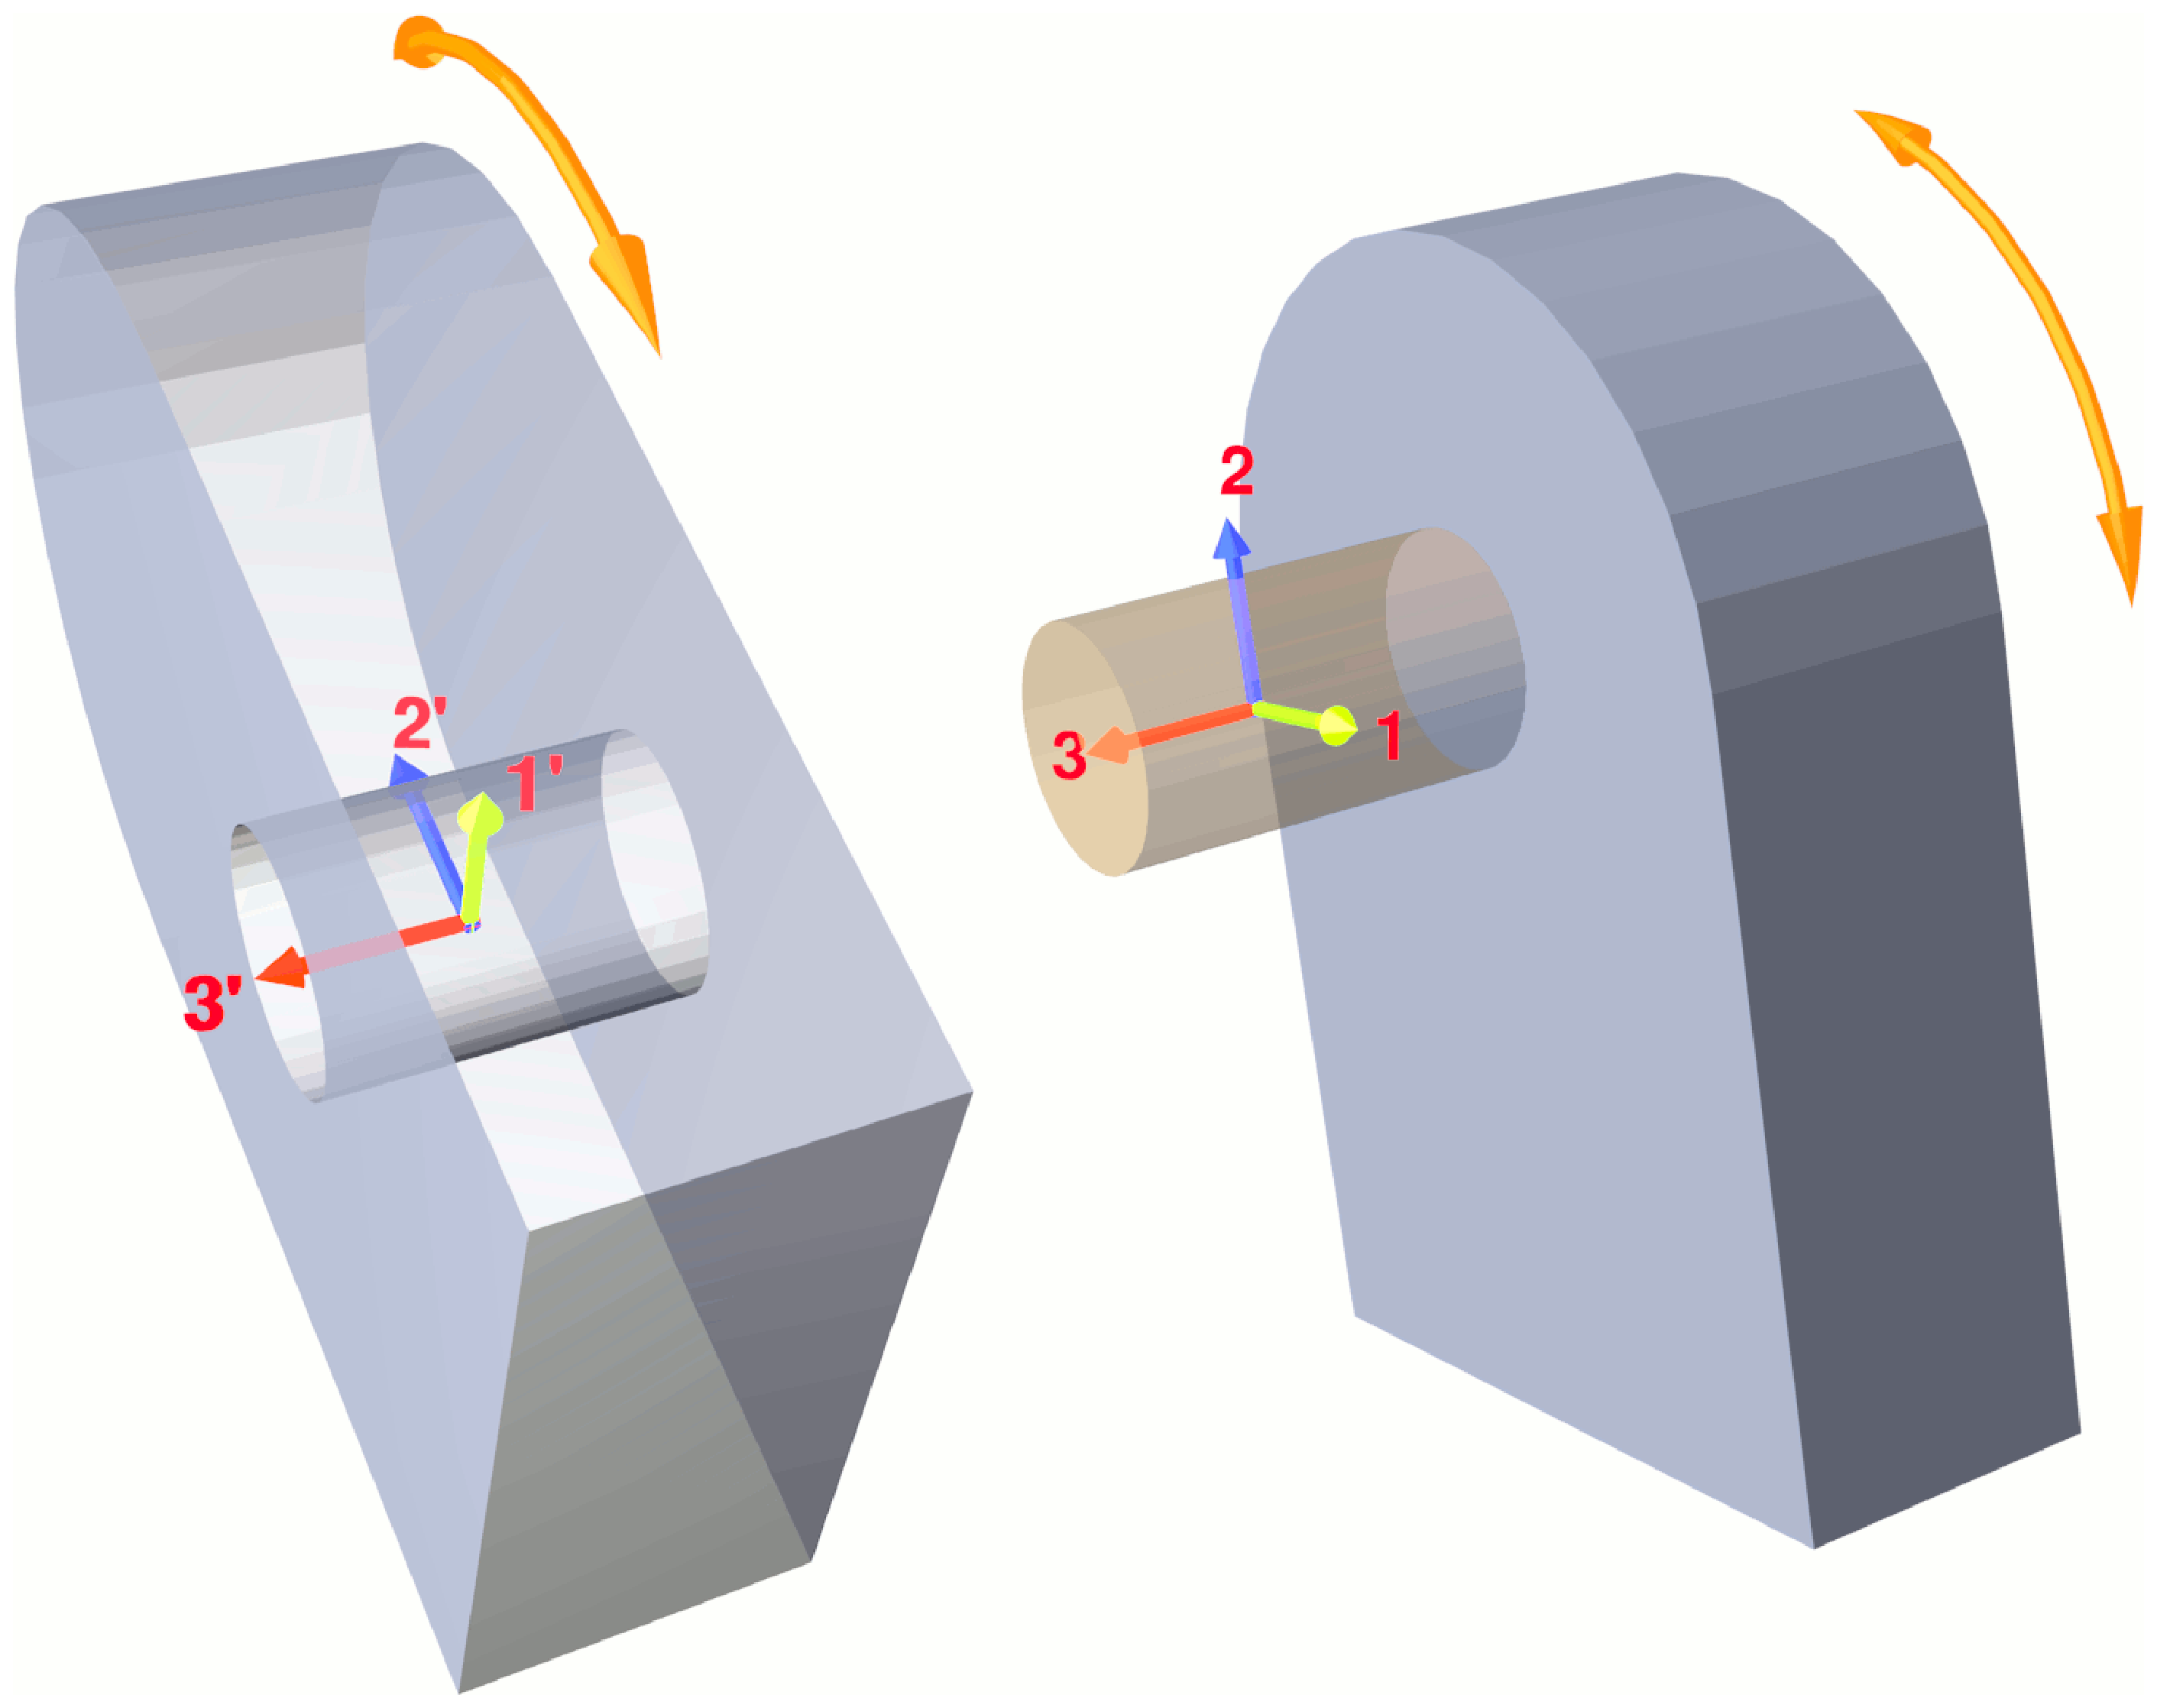
\includegraphics[width=.7\textwidth]{revHinge}
\caption{Revolute hinge.}
\label{fig:el:joint:REV}
\end{figure}

Note: this element can be thought of as the combination of a 
\hyperref{\kw{spherical hinge}}{\kw{spherical hinge} (see Section~}{)}{sec:EL:STRUCT:JOINT:SPHERICAL_HINGE},
that constrains the three components of the relative position
of the nodes, and of a
\hyperref{\kw{revolute rotation}}{\kw{revolute rotation} (see Section~}{)}{sec:EL:STRUCT:JOINT:REVOLUTE_ROTATION},
that constrains the relative orientation of the nodes so that only rotation
about a common axis is allowed.

\subsubsection{Rationale}
The rationale for having two statements to indicate the position
and orientation of the same entity is that the joint is supposed
to constrain the position and orientation of two points,
each attached to a node.
This is what is typically known from the geometry of the components
of a mechanism.

\subsubsection{Output}
The output occurs in the \texttt{.jnt} file, according to default joint output
for the first 13 columns; specific columns contain:
\begin{itemize}
\item columns 14--16: the so-called \emph{Euler} angles (in degrees)
	that describe the relative rotation; only the third component
	is relevant, the first two essentially indicate the accuracy
	of the rotation constraint;
\item column 17--19: the relative angular velocity; only the third component
	is relevant, the first two are zero.
\end{itemize}
If friction is present:
\begin{itemize}
\item column 20: the friction moment about the revolute axis;
\item subsequent columns: any friction model specific data (quite possibly the friction coefficient).
\end{itemize}

\subsubsection{Private Data}
The following data are available:
\begin{enumerate}
\item \kw{"rz"} relative rotation angle about revolute axis
\item \kw{"wz"} relative angular velocity about revolute axis
\item \kw{"Fx"} constraint reaction force in node 1 local direction 1
\item \kw{"Fy"} constraint reaction force in node 1 local direction 2
\item \kw{"Fz"} constraint reaction force in node 1 local direction 3
\item \kw{"Mx"} constraint reaction moment about node 1 local direction 1
\item \kw{"My"} constraint reaction moment about node 1 local direction 2
\item \kw{"Mz"} constraint reaction moment about node 1 local direction 3
\end{enumerate}

\subsubsection{Hints}
When wrapped by a \kw{driven} element, the following hints are honored:
\begin{itemize}
\item \kw{hinge\{1\}} the relative orientation of the joint
with respect to node 1 is reset;
\item \kw{hinge\{2\}} the relative orientation of the joint
with respect to node 2 is reset;
\item \kw{offset\{1\}} the offset of the joint
with respect to node 1 is reset;
\item \kw{offset\{2\}} the offset of the joint
with respect to node 2 is reset;
\item unrecognized hints are passed through to the friction model,
if any.
\end{itemize}




\subsection{Revolute pin}
\label{sec:EL:STRUCT:JOINT:REVOLUTE_PIN}
This joint only allows the absolute rotation of a node about
a given axis, which is axis 3 in the reference systems defined 
by the two \kw{orientation} statements.
%\begin{verbatim}
\begin{Verbatim}[commandchars=\\\{\}]
    \bnt{joint_type} ::= \kw{revolute pin}

    \bnt{joint_arglist} ::= 
        \bnt{node_label} ,
            \kw{position}, (\hty{Vec3}) \bnt{relative_offset}
            [ , \kw{orientation}, (\hty{OrientationMatrix}) \bnt{relative_orientation_matrix} ] ,
        \kw{position} , (\hty{Vec3}) \bnt{absolute_pin_position}
        [ , \kw{orientation} , (\hty{OrientationMatrix}) \bnt{absolute_pin_orientation_matrix} ]
        [ , \kw{initial theta} , \bnt{initial_theta} ]
\end{Verbatim}
%\end{verbatim}
Note: this is equivalent to a
\hyperref{\kw{revolute hinge}}{\kw{revolute hinge} (see Section~}{)}{sec:EL:STRUCT:JOINT:REVOLUTE_HINGE}
when one node is grounded.

\subsubsection{Private Data}
The following data are available:
\begin{enumerate}
\item \kw{"rz"} relative rotation angle about revolute axis
\item \kw{"wz"} relative angular velocity about revolute axis
\item \kw{"Fx"} constraint reaction force in node 1 local direction 1
\item \kw{"Fy"} constraint reaction force in node 1 local direction 2
\item \kw{"Fz"} constraint reaction force in node 1 local direction 3
\item \kw{"Mx"} constraint reaction moment about node 1 local direction 1
\item \kw{"My"} constraint reaction moment about node 1 local direction 2
\item \kw{"Mz"} constraint reaction moment about node 1 local direction 3
\end{enumerate}

\subsubsection{Hints}
When wrapped by a \kw{driven} element, the following hints are honored:
\begin{itemize}
\item \kw{hinge\{1\}} the relative orientation of the joint
with respect to the node is reset;
\item \kw{hinge\{0\}} the relative orientation of the joint
with respect to the absolute frame is reset;
\item \kw{offset\{1\}} the offset of the joint
with respect to the node is reset;
\item \kw{offset\{0\}} the offset of the joint
with respect to the absolute frame is reset;
\end{itemize}






\subsection{Revolute rotation}
\label{sec:EL:STRUCT:JOINT:REVOLUTE_ROTATION}
This joint allows the relative rotation of two nodes about
a given axis, which is axis 3 in the reference systems defined 
by the two \kw{orientation} statements.
The relative position is not constrained.
%\begin{verbatim}
\begin{Verbatim}[commandchars=\\\{\}]
    \bnt{joint_type} ::= \kw{revolute rotation}

    \bnt{joint_arglist} ::= 
        \bnt{node_1_label}
            [ , \kw{position} , (\hty{Vec3}) \bnt{relative_offset_1} ]
            [ , \kw{orientation} , (\hty{OrientationMatrix}) \bnt{relative_orientation_matrix_1} ] ,
        \bnt{node_2_label}
            [ , \kw{position} , (\hty{Vec3}) \bnt{relative_offset_2} ]
            [ , \kw{orientation} , (\hty{OrientationMatrix}) \bnt{relative_orientation_matrix_2} ]
\end{Verbatim}
%\end{verbatim}

\subsubsection{Rationale}
A revolute joint without position constraints; this joint, in conjunction
with an \kw{inline} joint, should be used to constrain, for example,
the two nodes of a hydraulic actuator.

\subsubsection{Private Data}
The following data are available:
\begin{enumerate}
\item \kw{"rz"} relative rotation angle about revolute axis
\item \kw{"wz"} relative angular velocity about revolute axis
\item \kw{"Mx"} constraint reaction moment about node 1 local direction 1
\item \kw{"My"} constraint reaction moment about node 1 local direction 2
\item \kw{"Mz"} constraint reaction moment about node 1 local direction 3
\end{enumerate}

\subsubsection{Hints}
When wrapped by a \kw{driven} element, the following hints are honored:
\begin{itemize}
\item \kw{hinge\{1\}} the relative orientation of the joint
with respect to node 1 is reset;
\item \kw{hinge\{2\}} the relative orientation of the joint
with respect to node 2 is reset;
\end{itemize}

\subsection{Rigid body displacement joint}
\label{sec:EL:STRUCT:JOINT:RIGID_BODY_DISP_JOINT}
\emph{Author: Reinhard Resch}

This element is a load distributing coupling constraint similar to NASTRAN's \texttt{RBE3} element.
However, it may be used also in the context of large deformations and large rotations.
It is intended mainly to provide an interface between solid elements, which are using \htmlref{\kw{structural displacement node}}{sec:NODE:STRUCTURAL}s with only three degrees of freedom,
and the large family of elements (e.g. joints, forces, ...) which can be used only for \htmlref{\kw{structural node}}{sec:NODE:STRUCTURAL}s with six degrees of freedom.

\begin{Verbatim}[commandchars=\\\{\}]
    \bnt{joint_type} ::= \kw{rigid body displacement joint}

    \bnt{joint_arglist} ::=
       (\ty{StructNode}) \bnt{node_label_master} ,
       (\ty{integer}) \bnt{slave_node_number} ,
       \bnt{slave_node_data}
       [ , \kw{alpha}, (\ty{real}) \bnt{alpha} ] ;

    \bnt{slave_node_data} :: =
       \bnt{one_slave_node_1}
       [ , ... ]
       [ , \bnt{one_slave_node_N} ];

    \bnt{one_slave_node_i} :: =
       (\ty{StructDispNode}) \bnt{node_label_slave_i}
       [ , \kw{position} , (\hty{Vec3}) \bnt{position_slave_node_i} ]    
       [ , \kw{weight} , (\ty{real}) \bnt{weight_slave_node_i} ]

\end{Verbatim}

\paragraph{Kinematics}
The position and orientation of the \nt{node\_label\_master} is constrained in a way, that it's following the weighted average
of the rigid body motion of a set of \nt{slave\_node\_number} slave nodes. But, no artificial stiffness will be added to the slave nodes.
Since the slave nodes do not have any rotational degrees of freedom, a minimum number of three non coincident slave nodes is required.
If the optional parameter \nt{position\_slave\_node} is present, it is used to compute the relative offset between \nt{node\_label\_slave}
and \nt{node\_label\_master}. Otherwise, the initial position of \nt{node\_label\_slave} is used to compute the offset.
\paragraph{Corner nodes of quadratic elements}
There is also an optional weighting factor \nt{weight\_slave\_node} per node, which may be used for second order solid elements in order to achieve a smooth stress distribution.
Negative values for \nt{weight\_slave\_node} are allowed (e.g. for corner nodes of quadratic hexahedrons), but the sum of all weighting factors must be always greater than zero.
See also section~\ref{sec:EL:SOLID:preprocessing} for an example on how to create a \kw{rigid body displacement joint} automatically from a Finite Element mesh.
\paragraph{Scaling}
The optional parameter \nt{alpha} may be used to scale the constraint equations in order to improve the condition number of the Jacobian matrix.
However, it has no effect on the result and the default value should be fine for most applications.

\subsubsection{Output}
The output occurs in the \texttt{.jnt} file, which contains the reaction force and reaction couple related to the \nt{node\_label\_master}.

\subsubsection{Private Data}
The following data is available:
\begin{enumerate}
\item \kw{"Fx"} reaction force at \nt{node\_label\_master} along \nt{node\_label\_master} axis 1
\item \kw{"Fy"} reaction force at \nt{node\_label\_master} along \nt{node\_label\_master} axis 2
\item \kw{"Fz"} reaction force at \nt{node\_label\_master} along \nt{node\_label\_master} axis 3

\item \kw{"Mx"} reaction moment at \nt{node\_label\_master} along \nt{node\_label\_master} axis 1
\item \kw{"My"} reaction moment at \nt{node\_label\_master} along \nt{node\_label\_master} axis 2
\item \kw{"Mz"} reaction moment at \nt{node\_label\_master} along \nt{node\_label\_master} axis 3

\item \kw{"fx"} reaction force at \nt{node\_label\_master} along global axis 1
\item \kw{"fy"} reaction force at \nt{node\_label\_master} along global axis 2
\item \kw{"fz"} reaction force at \nt{node\_label\_master} along global axis 3

\item \kw{"mx"} reaction moment at \nt{node\_label\_master} along global axis 1
\item \kw{"my"} reaction moment at \nt{node\_label\_master} along global axis 2
\item \kw{"mz"} reaction moment at \nt{node\_label\_master} along global axis 3
\end{enumerate}

\paragraph{Example.}
This example mimics an instance of NASTRAN's \texttt{RBE3} element.
\begin{Verbatim}
  begin: nodes;
    structural: 609, static, reference, ref_id_solid, null,
                             reference, ref_id_solid, eye,
                             reference, ref_id_solid, null,
                             reference, ref_id_solid, null;
    structural: 1, dynamic displacement,
                             reference, ref_id_solid, 5.1e+02,  1.0e+01, -1.0e+01,
                             reference, ref_id_solid, null;
    structural: 2, dynamic displacement,
                             reference, ref_id_solid, 5.1e+02,  -1.0e+01, -1.0e+01,
                             reference, ref_id_solid, null;
    ...
    structural: 8, dynamic displacement,
                             reference, ref_id_solid, 9.9e+02,  -1.0e+01, 1.0e+01,
                             reference, ref_id_solid, null;
  end: nodes;
  begin: elements;
     joint: 100, rigid body displacement joint,
            609, ## master node label
              8, ## eight slave nodes
              5, weight, 1.3333333333333348e+02, ## midside nodes
              6, weight, 1.3333333333333351e+02,
              7, weight, 1.3333333333333351e+02,
              9, weight, 1.3333333333333351e+02,
             13, weight, -3.3333333333333414e+01, ## corner nodes
             14, weight, -3.3333333333333428e+01,
             15, weight, -3.3333333333333421e+01,
             16, weight, -3.3333333333333421e+01;
   end: elements;
\end{Verbatim}


\subsection{Rod}\label{sec:EL:STRUCT:JOINT:ROD}
The \kw{rod} element represents a force between two nodes that depends
on the relative position and velocity of two points, each rigidly attached
to a \htmlref{\kw{structural node}}{sec:NODE:STRUCTURAL} with an optional offset.
The direction of the force is also based on the relative position
of the points: it is the line that passes through them.
If no offset is defined, the points are the nodes themselves.

The syntax is:
%\begin{verbatim}
\begin{Verbatim}[commandchars=\\\{\}]
    \bnt{joint_type} ::= \kw{rod}

    \bnt{joint_arglist} ::=
        \bnt{node_1_label} ,
            [ \kw{position} , (\hty{Vec3}) \bnt{relative_offset_1} , ]
        \bnt{node_2_label} , 
            [ \kw{position} , (\hty{Vec3}) \bnt{relative_offset_2} , ]
        \{ (\ty{real}) \bnt{rod_length} | \kw{from nodes} \}
        (\htybkw{ConstitutiveLaw}{1D}) \bnt{const_law}
\end{Verbatim}
%\end{verbatim}
\nt{rod\_length} is the distance between the points connected by the rod that represents the reference length of the rod (see $\ell_0$ below).
When the form \kw{from nodes} is used, such distance is computed considering the points connected by the rods, including the offsets if defined.

\subsubsection{Note on the use of the constitutive law}
The constitutive law \nt{const\_law} receives as input the rod axial strain
\begin{equation}
	\varepsilon = \frac{\ell - \ell_0}{\ell_0} = \cfrac{\ell}{\ell_0} - 1 ,
\end{equation}
where $l_0=\nt{rod\_length}$ and $l$ is the distance between the two points;
in case of viscous or viscoelastic constitutive law, the axial strain derivative
\begin{equation}
	\dot{\varepsilon} = \frac{\dot{\ell}}{\ell_0}
\end{equation}
is also used.
It returns the corresponding rod axial force,
\begin{displaymath}
	F = F\plbr{\frac{\ell - \ell_0}{\ell_0}, \frac{\dot{\ell}}{\ell_0}} .
\end{displaymath}
If a \nt{prestrain} $\varepsilon_p$ is defined,
it consists in an imposed value of the axial strain
that is subtracted from the geometrical strain
before being passed to the constitutive law;
if a \nt{prestress} $F_p$ is defined,
it consists in an imposed axial force value
that is added to the one obtained from the constitutive law,
namely
\begin{displaymath}
	% F = F_p + F\plbr{\frac{l - l_0}{l_0} - \varepsilon_p, \frac{\dot{l}}{l_0} - \dot{\varepsilon}_p} .
	F = F_p + F\plbr{\frac{\ell - \ell_0}{l_0} - \varepsilon_p, \frac{\dot{\ell}}{\ell_0}} .
\end{displaymath}
% FIXME: - \dot{\varepsilon}_p is not currently implemented

For example, a linear elastic constitutive law for the rod element
is defined as
\begin{displaymath}
	F = EA \frac{\ell - \ell_0}{\ell_0} ,
\end{displaymath}
where $EA$ is the axial stiffness of the rod.
The corresponding syntax would be:
\begin{verbatim}
    set: const real L_0 = 0.35;  # reference length
    set: const real EA = 7.0e+6; # axial stiffness
    joint: 99, rod,
        1, position, null,
        2, position, null,
        L_0,
        linear elastic, EA;
\end{verbatim}
To model a lumped spring of stiffness $K$, such that $F = K (\ell - \ell_0)$ and thus $EA = K \ell_0$, one needs to use
\begin{verbatim}
    set: const real L_0 = 0.35;  # reference length
    set: const real K = 2.0e+7;  # lumped spring stiffness
    joint: 99, rod,
        1, position, null,
        2, position, null,
        L_0,
        linear elastic, K*L_0;
\end{verbatim}
Similar considerations apply to the damping characteristic of a viscoelastic constitutive law:
\begin{verbatim}
    set: const real L_0 = 0.35;  # reference length
    set: const real K = 2.0e+7;  # lumped spring stiffness
    set: const real C = 2.0e+2;  # lumped damper characteristic
    joint: 99, rod,
        1, position, null,
        2, position, null,
        L_0,
        linear viscoelastic, K*L_0, C*L_0;
\end{verbatim}

For further details on the supported constitutive laws, 
see Section~\ref{sec:ConstitutiveLaw}.
%If the optional \kw{offset} keyword is used, the element falls through
%to the more general \kw{rod with offset};
%see also \kw{rod with offset}
%in Section~\ref{sec:EL:STRUCT:JOINT:ROD_WITH_OFFSET}.



\subsubsection{Use of ``current''}
When parsing the constitutive law, the following run-time computed values are made available
through the \kw{model::current}\texttt{(\bnt{string})} model namespace interface:
\begin{itemize}
\item
\nt{string}\texttt{ ::= }\kw{"L0"}:
the length of the rod \nt{rod\_length} as input by the user,
or computed from the distance between the points connected by the rod when \kw{from nodes} is used;

\item
\nt{string}\texttt{ ::= }\kw{"L"}: 
the length of the rod computed from the distance between the points connected by the rod;
identical to \kw{"L0"} when \kw{from nodes} is used.
\end{itemize}
For example, if one knows the value of $K$ and wants the axial stiffness
in a linear elastic constitutive law to reflect its dependence
on the reference length of the rod as computed from the initial configuration,
the following syntax does the trick:
\begin{verbatim}
    set: const real K = 2.e+7;
    # ...
    joint: 99, rod,
        1, position, null,
        2, position, null,
        from nodes,                             # compute length from nodes
        linear elastic, K*model::current("L0"); # compute EA as K*rod_length
\end{verbatim}



\subsubsection{Output}
The output occurs in the \texttt{.jnt} file, which contains:
\begin{itemize}
\item the label
\item the three components of the internal force in the reference frame
of the element (column 2, component $x$, contains the force)
\item the three components of the internal moment in the reference frame
of the element (always zero)
\item the three components of the internal force in the global
reference frame
\item the three components of the internal moment in the global
reference frame (always zero)
\item the length of the rod
\item the three components of the rod axis in the global reference frame
(a unit vector)
\item the length rate of the rod (derivative of length wrt/ time)
\item optional data appended by the constitutive law
\end{itemize}

\subsubsection{Private Data}
The following data are available:
\begin{enumerate}
\item \kw{"F"} force between the two nodes/connection points
\item \kw{"l"} distance between the two nodes/connection points
\item \kw{"lP"} distance rate between the two nodes/connection points
\end{enumerate}
The rod joint can also give access the private data provided 
by the constitutive law.
It is accessed by prefixing the name of the data with the string
\kw{"constitutiveLaw."}; see the specific constitutive law
description of the available data in Section~\ref{sec:ConstitutiveLaw}.





\subsection{Rod with offset}
\label{sec:EL:STRUCT:JOINT:ROD_WITH_OFFSET}
The syntax is:
%\begin{verbatim}
\begin{Verbatim}[commandchars=\\\{\}]
    \bnt{joint_type} ::= \kw{rod with offset}

    \bnt{joint_arglist} ::=
        \bnt{node_1_label} ,
            (\hty{Vec3}) \bnt{relative_offset_1} ,
        \bnt{node_2_label} ,
            (\hty{Vec3}) \bnt{relative_offset_2} ,
        \{ (\ty{real}) \bnt{rod_length} | \kw{from nodes} \} ,
        (\htybkw{ConstitutiveLaw}{1D}) \bnt{const_law}
\end{Verbatim}
%\end{verbatim}
Analogous to the \kw{rod} joint with the optional offsets;
see Section~\ref{sec:EL:STRUCT:JOINT:ROD} for details.

\subsection{Screw joint}
\label{sec:screw}
This joint models a screw, aligned with axis 3 defined by the
first node \kw{orientation} statement. 
Friction, if declared, can prevent the relative
motion.
\begin{Verbatim}[commandchars=\\\{\}]
    \bnt{joint_type} ::= \kw{screw}

    \bnt{joint_arglist} ::= 
        \bnt{node_1_label} ,
            [ \kw{position} , (\hty{Vec3}) \bnt{relative_offset_1} , ]
            [ \kw{orientation} , (\hty{OrientationMatrix}) \bnt{relative_orientation_matrix_1} , ]
        \bnt{node_2_label} ,
            [ \kw{offset} , (\hty{Vec3}) \bnt{relative_offset_2} , ]
        \kw{pitch} , \bnt{screw_pitch_angle}
	[ , \kw{friction} , 
            \bnt{friction_model} , 
            \bnt{shape_function} ]
\end{Verbatim}
The \hty{shape function} should be a \kw{screw joint} shape function.
\subsubsection{Output}
The output occurs in the \texttt{.jnt} file, according to default joint output
for the first 13 columns; specific columns contain:
\begin{itemize}
\item column 14: the overall relative rotation angle between
        the two nodes, in degrees, along the prescribed screw direction,
\item colums 15--17: the relative rotation vector
	$\mathrm{ax}(\log(\T{R}_{1}^T\T{R}_2)$;
\end{itemize}
If friction is present:
\begin{itemize}
\item column 18: the relative velocity $v$ along the friction force direction;
\item column 19: the friction-induced moment value about the screw axis;
\item subsequent columns: any friction model specific data 
      (quite possibly the friction coefficient).
\end{itemize}

\subsection{Spherical hinge}
\label{sec:EL:STRUCT:JOINT:SPHERICAL_HINGE}
This joint constrains the relative position of two nodes;
the relative orientation is not constrained.
%\begin{verbatim}
\begin{Verbatim}[commandchars=\\\{\}]
    \bnt{joint_type} ::= \kw{spherical hinge}

    \bnt{joint_arglist} ::= 
        \bnt{node_1_label} ,
            [ \kw{position} , (\hty{Vec3}) \bnt{relative_offset_1} , ]
            [ \kw{orientation} , (\hty{OrientationMatrix}) \bnt{relative_orientation_matrix_1} , ]
        \bnt{node_2_label}
            [ , \kw{position} , (\hty{Vec3}) \bnt{relative_offset_2} ]
            [ , \kw{orientation} , (\hty{OrientationMatrix}) \bnt{relative_orientation_matrix_2} ]
\end{Verbatim}
%\end{verbatim}
The joint is shown in Figure~\ref{fig:el:joint:SPHERE} where the axes shown are the those obtained after having applied the \nt{relative\_offset} and \nt{relative\_orientation\_matrix} transformations to the coordinates of \nt{node\_1} and \nt{node\_2}.
\begin{figure}
\centering
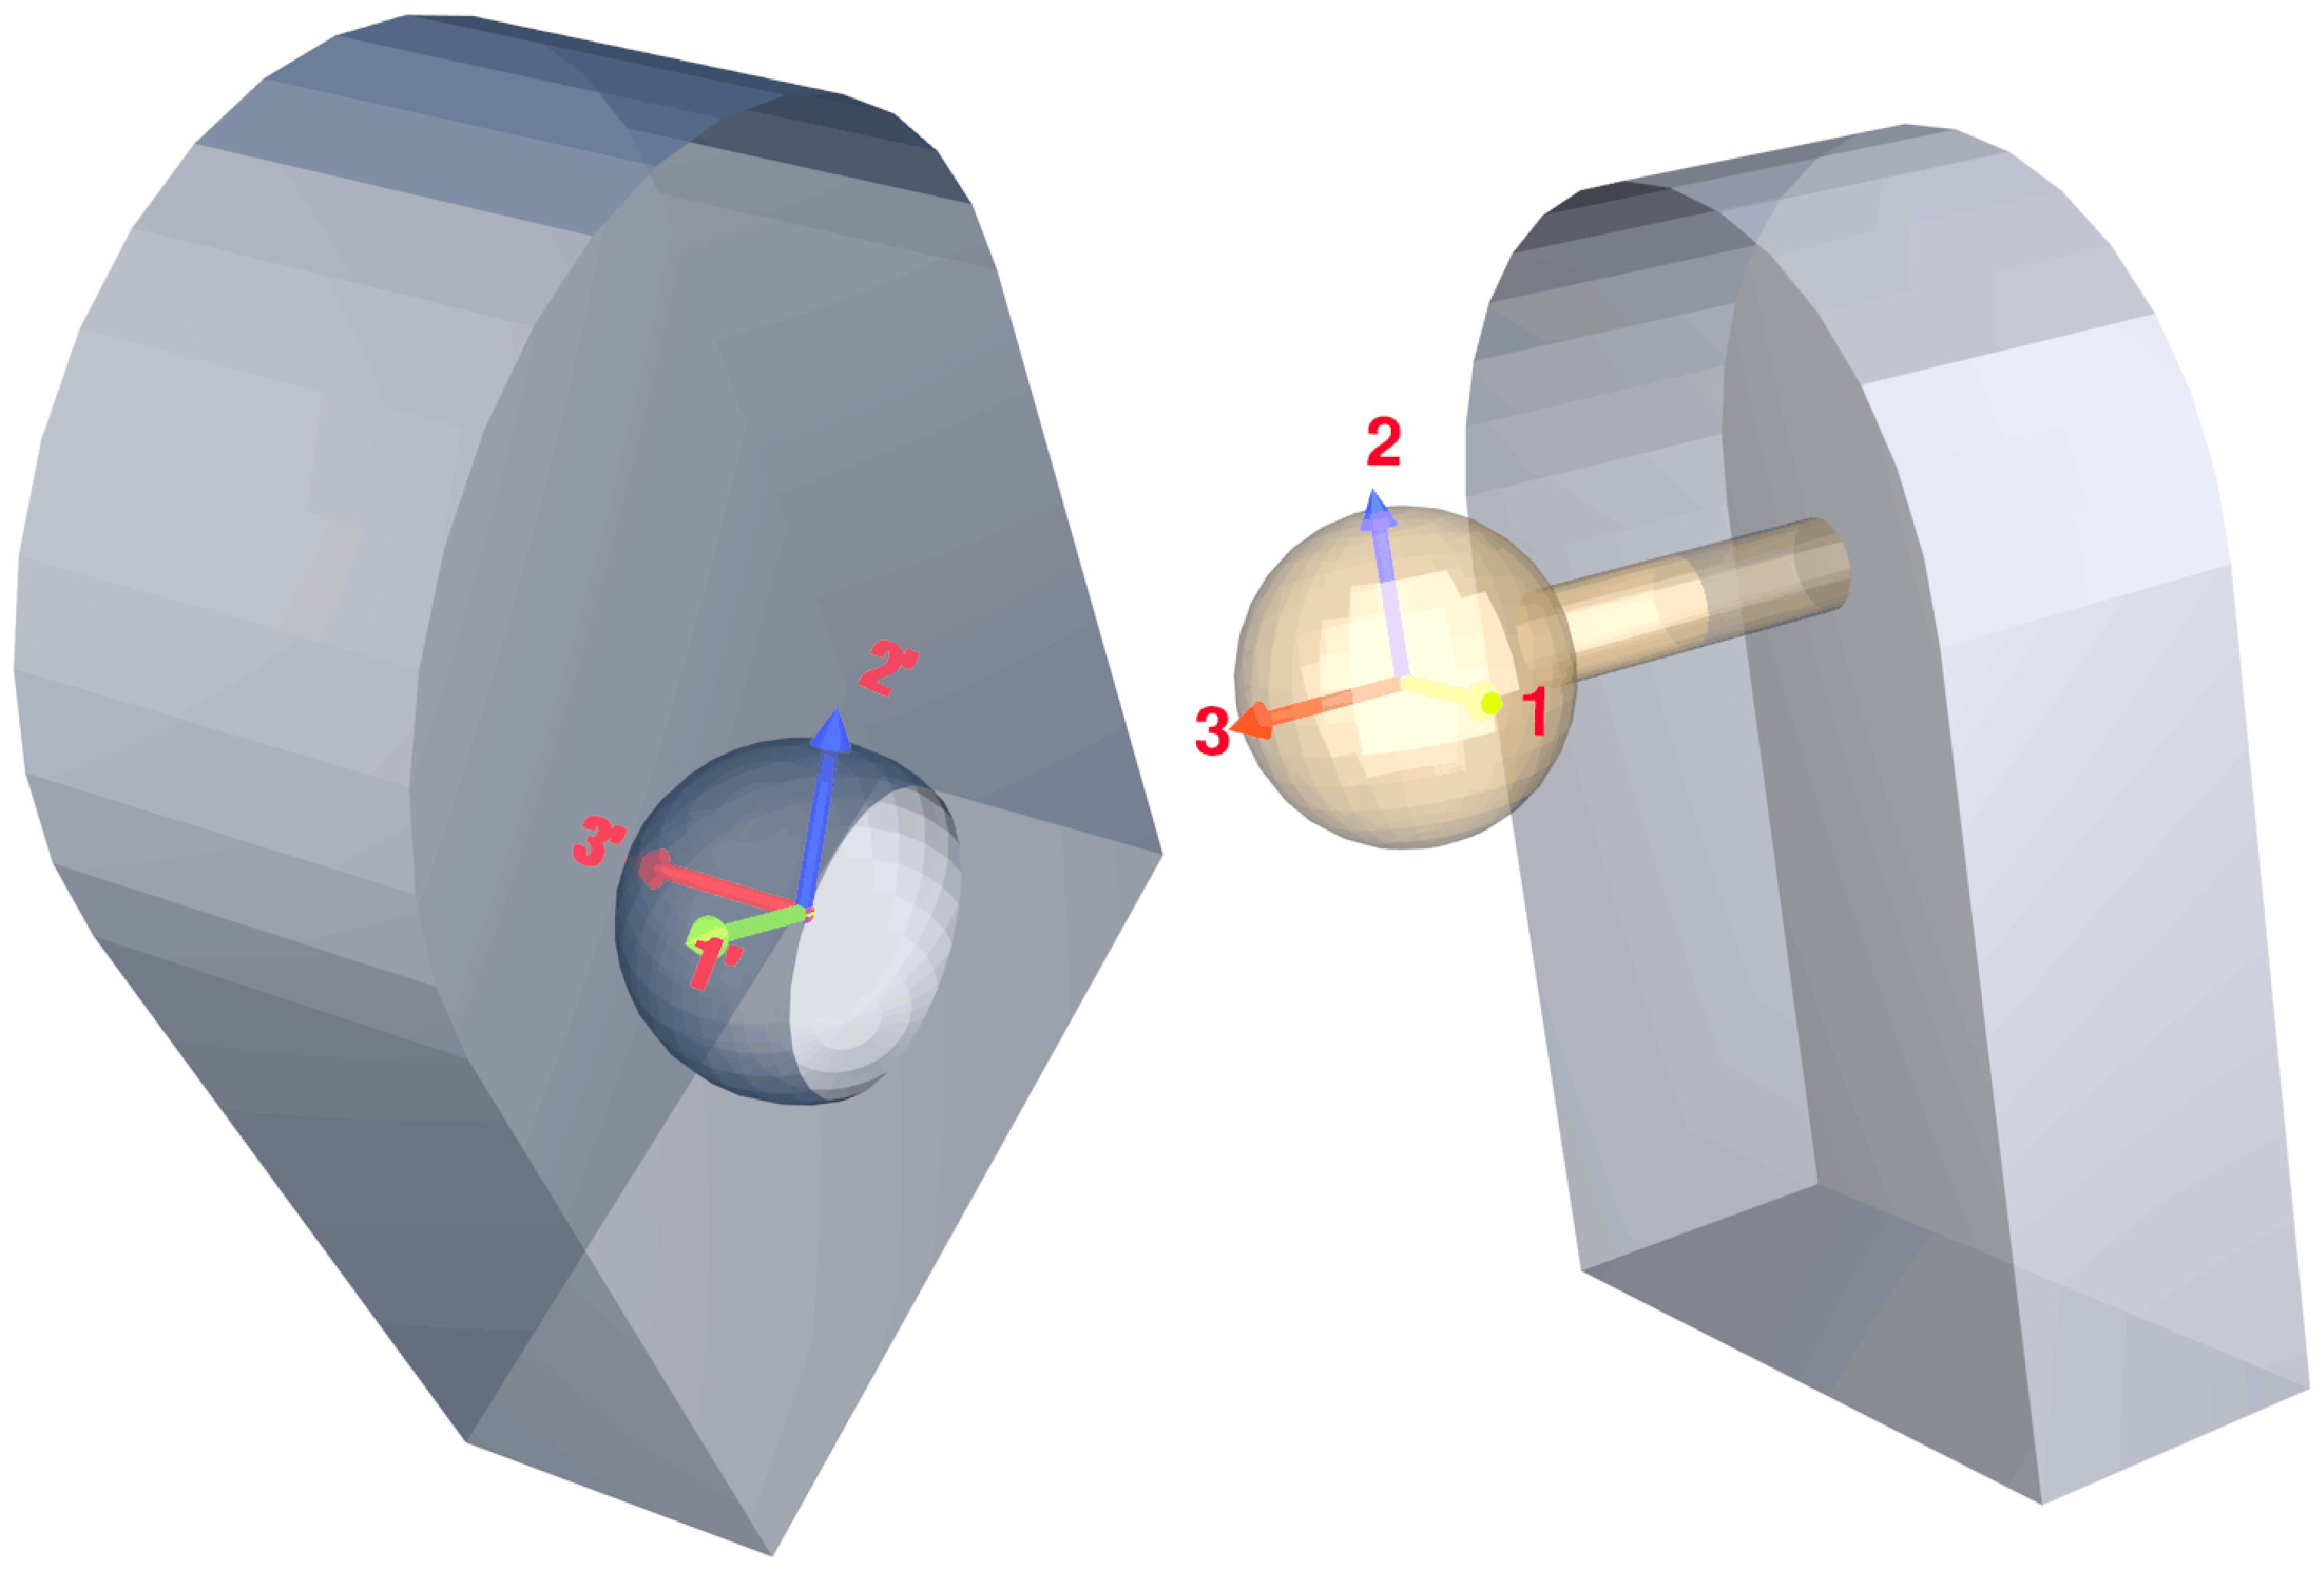
\includegraphics[width=.7\textwidth]{spherHinge}
\caption{Spherical hinge.}
\label{fig:el:joint:SPHERE}
\end{figure}
Note: the orientation matrix, set by means of the \kw{orientation} keyword,
is used for output purposes only. 
A default identity matrix is assumed.

\subsubsection{Hints}
When wrapped by a \kw{driven} element, the following hints are honored:
\begin{itemize}
\item \kw{offset\{1\}} the offset of the joint
with respect to node 1 is reset;
\item \kw{offset\{2\}} the offset of the joint
with respect to node 2 is reset;
\end{itemize}

\subsection{Spherical pin}
This joint constrains the absolute position of a node;
the relative orientation is not constrained.
%\begin{verbatim}
\begin{Verbatim}[commandchars=\\\{\}]
    \bnt{joint_type} ::= \kw{spherical pin}

    \bnt{joint_arglist} ::=
        \bnt{node_label} ,
            [ \kw{position} , (\hty{Vec3}) \bnt{relative_offset} , ]
            [ \kw{orientation} , (\hty{OrientationMatrix}) \bnt{relative_orientation} , ]
        \kw{position} , (\hty{Vec3}) \bnt{absolute_pin_position}
        [ , \kw{orientation} , \bnt{absolute_orientation} ]   
\end{Verbatim}
%\end{verbatim}
Note: this is equivalent to a
\hyperref{\kw{spherical hinge}}{\kw{spherical hinge} (see Section~}{)}{sec:EL:STRUCT:JOINT:SPHERICAL_HINGE}
when one node is grounded.
An alternative way to model a grounded spherical hinge requires
the use of another node, clamped by a \kw{clamp} joint.



\subsection{Total equation}
\label{sec:EL:STRUCT:JOINT:TOTAL_EQUATION}
\emph{Original implementation: Alessandro Fumagalli, Marco Morandini.}

See also
\hyperref{\kw{total reaction}}{\kw{total reaction} (see Section~}{)}{sec:EL:STRUCT:JOINT:TOTAL_REACTION}.
See \cite{FUMAGALLI-CND-2011}.
TODO



\subsection{Total joint}
\label{sec:EL:STRUCT:JOINT:TOTAL_JOINT}
\emph{Original implementation: Alessandro Fumagalli; \\
Review: Pierangelo Masarati.}

See \cite{MASARATI-TOTALJ}.
This element allows to arbitrarily constrain specific components
of the relative position and orientation of two nodes.
The value of the constrained components of the relative position
and orientation can be imposed by means of drives.
As such, this element allows to mimic the behavior of most
ideal constraints that connect two nodes.
%\begin{verbatim}
\begin{Verbatim}[commandchars=\\\{\}]
    \bnt{joint_type} ::= \kw{total joint}

    \bnt{joint_arglist} ::=
        \bnt{node_1_label}
            [ , \kw{position} , (\hty{Vec3}) \bnt{relative_offset_1} ]
            [ , \kw{position orientation} , (\hty{OrientationMatrix}) \bnt{rel_pos_orientation_1} ]
            [ , \kw{rotation orientation} , (\hty{OrientationMatrix}) \bnt{rel_rot_orientation_1} ]
        , \bnt{node_2_label}
            [ , \kw{position} , (\hty{Vec3}) \bnt{relative_offset_2} ]
            [ , \kw{position orientation} , (\hty{OrientationMatrix}) \bnt{rel_pos_orientation_2} ]
            [ , \kw{rotation orientation} , (\hty{OrientationMatrix}) \bnt{rel_rot_orientation_2} ]
        [ , \kw{position constraint} ,
            \bnt{position_status} , \bnt{position_status} , \bnt{position_status} ,
            (\htybty{TplDriveCaller}{Vec3}) \bnt{imposed_relative_position} ]
        [ , \kw{orientation constraint} ,
            \bnt{orientation_status} , \bnt{orientation_status} , \bnt{orientation_status} ,
            (\htybty{TplDriveCaller}{Vec3}) \bnt{imposed_relative_rotation} ]

    \bnt{position_status} ::=
            \{ \kw{inactive} | \kw{active} | \kw{position} | \kw{velocity} | \bnt{status} \}

    \bnt{orientation_status} ::=
            \{ \kw{inactive} | \kw{active} | \kw{rotation} | \kw{angular velocity} | \bnt{status} \}
\end{Verbatim}
%\end{verbatim}
The relative position imposed by the \kw{position constraint}
is imposed in a reference frame rigidly attached to the first node,
in the optional offset \nt{relative\_offset\_1},
and optionally further oriented by the \nt{rel\_pos\_orientation\_1}
matrix.

The relative orientation imposed by the \kw{orientation constraint}
is imposed in a reference frame rigidly attached to the first node,
optionally further oriented by the \nt{rel\_rot\_orientation\_1}
matrix.
It consists in the Euler vector that expresses
the imposed relative orientation, in radian.

The keyword \kw{active} means that the constraint is active
with respect to that component of relative motion,
so the related motion component is constrained,
while \kw{inactive} means that the constraint is not active
with respect of that component of relative motion,
so the related motion component is not constrained.
Otherwise, a boolean can be provided in \nt{status} to indicate
that the degree of constraint is either inactive (0) or active (1);
this may be useful, for instance, to make constraint activation
conditional in parametric input files.
The same applies to the status of the components of the impose orientation.

If a component of relative position or orientation is active,
the corresponding component of the imposed position or orientation
is enforced, otherwise it is ignored;
however, the complete three-dimensional vectors of the imposed relative
position or orientation must be provided.

When the \kw{position constraint} is enforced, the keyword \kw{active}
is equivalent to \kw{position}; if the keyword \kw{velocity} is used,
the constraint imposes the velocity of that component of the relative position,
resulting in a non-holonomic constraint.

Similarly, when the \kw{orientation constraint} is enforced,
the keyword \kw{active} is equivalent to \kw{rotation};
if the keyword \kw{angular velocity} is used,
the constraint imposed the angular velocity of that component
of the relative orientation, resulting in a non-holonomic constraint.

\subsubsection{Output}
The output occurs in the \texttt{.jnt} file, which contains:
\begin{itemize}
\item column 1: the label

\item columns 2--4: the three components of the internal force in the reference frame of the element

\item columns 5--7: the three components of the internal moment in the reference frame of the element

\item columns 8--10: the three components of the internal force in the global reference frame

\item columns 11--13: the three components of the internal moment in the global reference frame

\item columns 14--16: the three components of the relative displacement in the reference frame of the element

\item columns 17--19: the three components of the relative rotation vector in the reference frame of the element

\item columns 20--22: the three components of the relative velocity in the reference frame of the element

\item columns 23--25: the three components of the relative angular velocity in the reference frame of the element

\end{itemize}

\subsubsection{Private Data}
The following data are available:
\begin{enumerate}
\item \kw{"px"} relative position along node 1 position orientation axis 1
\item \kw{"py"} relative position along node 1 position orientation axis 2
\item \kw{"pz"} relative position along node 1 position orientation axis 3

\item[-] alternatively, \kw{"X[i]"}, \kw{i} = 1, 2, 3, relative position along node 1 position orientation axis \kw{i}

\item \kw{"rx"} relative orientation about node 1 rotation orientation axis 1
\item \kw{"ry"} relative orientation about node 1 rotation orientation axis 2
\item \kw{"rz"} relative orientation about node 1 rotation orientation axis 3

\item[-] alternatively, \kw{"Phi[i]"}, \kw{i} = 1, 2, 3, relative orientation about node 1 rotation orientation axis \kw{i}

\item \kw{"Fx"} reaction force along node 1 position orientation axis 1
\item \kw{"Fy"} reaction force along node 1 position orientation axis 2
\item \kw{"Fz"} reaction force along node 1 position orientation axis 3

\item[-] alternatively, \kw{"f[i]"}, \kw{i} = 1, 2, 3, reaction force along node 1 position orientation axis \kw{i}

\item \kw{"Mx"} reaction moment about node 1 rotation orientation axis 1
\item \kw{"My"} reaction moment about node 1 rotation orientation axis 2
\item \kw{"Mz"} reaction moment about node 1 rotation orientation axis 3

\item[-] alternatively, \kw{"m[i]"}, \kw{i} = 1, 2, 3, reaction moment about node 1 rotation orientation axis \kw{i}

\item \kw{"dx"} imposed relative position along node 1 position orientation axis 1
\item \kw{"dy"} imposed relative position along node 1 position orientation axis 2
\item \kw{"dz"} imposed relative position along node 1 position orientation axis 3

\item \kw{"tx"} imposed relative orientation about node 1 rotation orientation axis 1
\item \kw{"ty"} imposed relative orientation about node 1 rotation orientation axis 2
\item \kw{"tz"} imposed relative orientation about node 1 rotation orientation axis 3

\item \kw{"vx"} relative velocity along node 1 position orientation axis 1
\item \kw{"vy"} relative velocity along node 1 position orientation axis 2
\item \kw{"vz"} relative velocity along node 1 position orientation axis 3

\item[-] alternatively, \kw{"V[i]"}, \kw{i} = 1, 2, 3, relative velocity along node 1 position orientation axis \kw{i}

\item \kw{"wx"} relative angular velocity about node 1 rotation orientation axis 1
\item \kw{"wy"} relative angular velocity about node 1 rotation orientation axis 2
\item \kw{"wz"} relative angular velocity about node 1 rotation orientation axis 3

\item[-] alternatively, \kw{"Omega[i]"}, \kw{i} = 1, 2, 3, relative angular velocity about node 1 rotation orientation axis \kw{i}
\end{enumerate}

\subsubsection{Hints}
When wrapped by a \kw{driven} element, the following hints are honored:
\begin{itemize}
\item \kw{offset\{1\}} the offset of the joint
with respect to node 1 is reset;
\item \kw{offset\{2\}} the offset of the joint
with respect to node 2 is reset;
\item \kw{position-hinge\{1\}} the relative orientation
of the relative position constraint with respect to node 1 is reset;
\item \kw{position-hinge\{2\}} the relative orientation 
of the relative position constraint with respect to node 2 is reset;
\item \kw{orientation-hinge\{1\}} the relative orientation
of the relative orientation constraint with respect to node 1 is reset;
\item \kw{orientation-hinge\{2\}} the relative orientation 
of the relative orientation constraint with respect to node 2 is reset;
\item \kw{position-drive3} resets the relative position drive;
the hint is passed to the Vec3 drive hint parser.
\item \kw{orientation-drive3} resets the relative orientation drive;
the hint is passed to the Vec3 drive hint parser.
\end{itemize}



\paragraph{Example.} \
This example mimicks an instance of NASTRAN's \texttt{RBE2} element
that constrains displacement in $x$ and $y$, and rotation about $z$:
\begin{verbatim}
    set: const integer EID = 100;
    set: const integer GN = 200;
    set: const integer GM1 = 300;

    # ...

    # $.......2.......3.......4.......5.......
    # RBE2    EID     GN      CM      GM1
    joint: EID, total joint,
        GN,
            position, reference, node, null,
            position orientation, reference, node, eye,
            rotation orientation, reference, node, eye,
        GM1,
            position, reference, other node, null,
            position orientation, reference, other node, eye,
            rotation orientation, reference, other node, eye,
         position constraint,
            active,   # "active" if CM includes "1"; "inactive" otherwise
            active,   # "active" if CM includes "2"; "inactive" otherwise
            inactive, # "active" if CM includes "3"; "inactive" otherwise
            null,
         orientation constraint,
            inactive, # "active" if CM includes "4"; "inactive" otherwise
            inactive, # "active" if CM includes "5"; "inactive" otherwise
            active,   # "active" if CM includes "6"; "inactive" otherwise
            null;
\end{verbatim}



\subsection{Total pin joint}
This element allows to arbitrarily constrain specific components
of the absolute position and orientation of a node.
The value of the constrained components of the absolute position
and orientation can be imposed by means of drives.
As such, this element allows to mimic the behavior of most
ideal constraints that ground one node.
\label{sec:EL:STRUCT:JOINT:TOTAL_PIN_JOINT}
%\begin{verbatim}
\begin{Verbatim}[commandchars=\\\{\}]
    \bnt{joint_type} ::= \kw{total pin joint}

    \bnt{joint_arglist} ::=
        \bnt{node_label}
            [ , \kw{position} , (\hty{Vec3}) \bnt{relative_offset} ]
            [ , \kw{position orientation} , (\hty{OrientationMatrix}) \bnt{rel_pos_orientation} ]
            [ , \kw{rotation orientation} , (\hty{OrientationMatrix}) \bnt{rel_rot_orientation} ]
        [ , \kw{position} , (\hty{Vec3}) \bnt{absolute position} ]
        [ , \kw{position orientation} , (\hty{OrientationMatrix}) \bnt{abs_pos_orientation} ]
        [ , \kw{rotation orientation} , (\hty{OrientationMatrix}) \bnt{abs_rot_orientation} ]
        [ , \kw{position constraint} ,
            \bnt{position_status} , \bnt{position_status} , \bnt{position_status} ,
            (\htybty{TplDriveCaller}{Vec3}) \bnt{imposed_absolute_position} ]
        [ , \kw{orientation constraint} ,
            \bnt{orientation_status} , \bnt{orientation_status} , \bnt{orientation_status} ,
            (\htybty{TplDriveCaller}{Vec3}) \bnt{imposed_absolute_rotation} ]

    \bnt{position_status} ::=
            \{ \kw{inactive} | \kw{active} | \kw{position} | \kw{velocity} | \bnt{status} \}

    \bnt{orientation_status} ::=
            \{ \kw{inactive} | \kw{active} | \kw{rotation} | \kw{angular velocity} | \bnt{status} \}
\end{Verbatim}
%\end{verbatim}
The non-holonomic variant is not implemented yet.

\subsubsection{Output}
The output occurs in the \texttt{.jnt} file, which contains:
\begin{itemize}
\item column 1: the label

\item columns 2--4: the three components of the internal force in the reference frame of the element

\item columns 5--7: the three components of the internal moment in the reference frame of the element

\item columns 8--10: the three components of the internal force in the global reference frame

\item columns 11--13: the three components of the internal moment in the global reference frame

\item columns 14--16: the three components of the absolute displacement in the reference frame of the element

\item columns 17--19: the three components of the absolute rotation vector in the reference frame of the element

\item columns 20--22: the three components of the absolute velocity in the reference frame of the element

\item columns 23--25: the three components of the absolute angular velocity in the reference frame of the element

\end{itemize}

\subsubsection{Private Data}
The following data are available:
\begin{enumerate}
\item \kw{"px"} absolute position along absolute position orientation axis 1
\item \kw{"py"} absolute position along absolute position orientation axis 2
\item \kw{"pz"} absolute position along absolute position orientation axis 3

\item[-] alternatively, \kw{"X[i]"}, \kw{i} = 1, 2, 3, absolute position along absolute position orientation axis \kw{i}

\item \kw{"rx"} absolute orientation about absolute rotation orientation axis 1
\item \kw{"ry"} absolute orientation about absolute rotation orientation axis 2
\item \kw{"rz"} absolute orientation about absolute rotation orientation axis 3

\item[-] alternatively, \kw{"Phi[i]"}, \kw{i} = 1, 2, 3, absolute orientation about absolute rotation orientation axis \kw{i}

\item \kw{"Fx"} reaction force along absolute position orientation axis 1
\item \kw{"Fy"} reaction force along absolute position orientation axis 2
\item \kw{"Fz"} reaction force along absolute position orientation axis 3

\item[-] alternatively, \kw{"f[i]"}, \kw{i} = 1, 2, 3, reaction force along absolute position orientation axis \kw{i}

\item \kw{"Mx"} reaction moment about absolute rotation orientation axis 1
\item \kw{"My"} reaction moment about absolute rotation orientation axis 2
\item \kw{"Mz"} reaction moment about absolute rotation orientation axis 3

\item[-] alternatively, \kw{"m[i]"}, \kw{i} = 1, 2, 3, reaction moment about absolute rotation orientation axis \kw{i}

\item \kw{"dx"} imposed absolute position along absolute position orientation axis 1
\item \kw{"dy"} imposed absolute position along absolute position orientation axis 2
\item \kw{"dz"} imposed absolute position along absolute position orientation axis 3

\item \kw{"tx"} imposed absolute orientation about absolute rotation orientation axis 1
\item \kw{"ty"} imposed absolute orientation about absolute rotation orientation axis 2
\item \kw{"tz"} imposed absolute orientation about absolute rotation orientation axis 3

\item \kw{"vx"} absolute velocity along absolute position orientation axis 1
\item \kw{"vy"} absolute velocity along absolute position orientation axis 2
\item \kw{"vz"} absolute velocity along absolute position orientation axis 3

\item[-] alternatively, \kw{"V[i]"}, \kw{i} = 1, 2, 3, absolute velocity along absolute position orientation axis \kw{i}

\item \kw{"wx"} absolute angular velocity about absolute rotation orientation axis 1
\item \kw{"wy"} absolute angular velocity about absolute rotation orientation axis 2
\item \kw{"wz"} absolute angular velocity about absolute rotation orientation axis 3

\item[-] alternatively, \kw{"Omega[i]"}, \kw{i} = 1, 2, 3, absolute angular velocity about absolute rotation orientation axis \kw{i}
\end{enumerate}

\subsubsection{Hints}
When wrapped by a \kw{driven} element, the following hints are honored:
\begin{itemize}
\item \kw{offset\{1\}} the offset of the joint
with respect to the node is reset;
\item \kw{offset\{0\}} the absolute position of the joint
is reset;
\item \kw{position-hinge\{1\}} the relative orientation
of the absolute position constraint with respect to the node is reset;
\item \kw{position-hinge\{0\}} the absolute orientation 
of the absolute position constraint is reset;
\item \kw{orientation-hinge\{1\}} the relative orientation
of the absolute orientation constraint with respect to the node is reset;
\item \kw{orientation-hinge\{0\}} the absolute orientation 
of the absolute orientation constraint is reset;
\item \kw{position-drive3} resets the absolute position drive;
the hint is passed to the Vec3 drive hint parser.
\item \kw{orientation-drive3} resets the absolute orientation drive;
the hint is passed to the Vec3 drive hint parser.
\end{itemize}
Using \kw{hints} with a \kw{total pin joint} may be tricky.
For example, when the \kw{position constraint} must be modified,
it is important to understand what this field indicates.
In the case of the \kw{total pin joint}, it indicates
the relative position of the point attached to the node and expressed by the first \kw{position} keyword
with respect to the absolute position of the point expressed by the second \kw{position} keyword.

Let us assume that the \kw{structural node} labeled \texttt{NODE1} is defined in a given initial position, \texttt{\{X0, Y0, Z0\}}.
During the analysis, the position of the node changes.  At time \texttt{T1}, the node is ``grabbed''
by a \kw{total pin joint}, which prescribes a given \emph{displacement} from the location at which the node is grabbed.
The syntax would be
\begin{verbatim}
    driven: 30, string, "Time >= T1",
        hint, "position-drive3{array, 2,
            # first vector, position of node at time T1
            model::xposition(NODE1) - X0,
                    model::yposition(NODE1) - Y0,
                    model::zposition(NODE1) - Z0,
                const, 1.,
            # second vector, prescribed displacement
            1., 0., 0.,
                cosine, T1, 2*pi, 9., half, 0.
            }",
    joint: 30, total pin joint,
        NODE1,
            position, reference, global, X0, Y0, Z0,
            position orientation, reference, global, eye,
            rotation orientation, reference, global, eye,
        # ground
            # reference point on ground coincident with node initial position
            position, reference, global, X0, Y0, Z0,
            position orientation, reference, global, eye,
            rotation orientation, reference, global, eye,
        position constraint, active, active, active,
            null, # irrelevant, will be overridden by hint
        orientation constraint, inactive, inactive, inactive,
            null;
\end{verbatim}
That is, an array of 3D \kw{template drive callers}, i.e.\ the sum of 2 vectors, needs to be created.
The first drive caller is the result of computing the difference between the position
of the node at the current time step and the initial position; it is a constant vector.
The second drive caller is the prescribed displacement from the position of the node at time \texttt{T1}.

An alternative way to produce the same result is to define the prescribed relative displacement in terms of an absolute displacement, i.e.
\begin{verbatim}
    driven: 30, string, "Time >= T1",
        hint, "position-drive3{array, 2,
            # first vector, position of node at time T1
            model::xposition(NODE1), model::yposition(NODE1), model::zposition(NODE1),
                const, 1.,
            # second vector, prescribed displacement
            1., 0., 0.,
                cosine, T1, 2*pi, 9., half, 0.
            }",
    joint: 30, total pin joint,
        NODE1,
            position, reference, global, X0, Y0, Z0,
            position orientation, reference, global, eye,
            rotation orientation, reference, global, eye,
        # ground
            # reference point on ground in origin rather than node initial position
            position, reference, global, null,
            position orientation, reference, global, eye,
            rotation orientation, reference, global, eye,
        position constraint, active, active, active,
            null, # irrelevant, will be overridden by hint
        orientation constraint, inactive, inactive, inactive,
            null;
\end{verbatim}
Notice that in both cases the prescribed relative position, in the definition of the \kw{total pin joint},
is irrelevant, since it will be overridden by that defined in the \kw{hint}.
As such, an arbitrary value, e.g.\ \kw{null}, is used.



\subsection{Total reaction}
\label{sec:EL:STRUCT:JOINT:TOTAL_REACTION}
\emph{Original implementation: Alessandro Fumagalli, Marco Morandini.}

See also 
\hyperref{\kw{total equation}}{\kw{total equation} (see Section~}{)}{sec:EL:STRUCT:JOINT:TOTAL_EQUATION}.
TODO




\subsection{Universal hinge}
\label{sec:EL:STRUCT:JOINT:UNIVERSAL_HINGE}
Deprecated in favour of the
\hyperref{\kw{Cardano hinge}}{\kw{Cardano hinge} (see Section~}{)}{sec:EL:STRUCT:JOINT:CARDANO_HINGE}.



\subsection{Universal pin}
\label{sec:EL:STRUCT:JOINT:UNIVERSAL_PIN}
Deprecated in favour of the
\hyperref{\kw{Cardano pin}}{\kw{Cardano pin} (see Section~}{)}{sec:EL:STRUCT:JOINT:CARDANO_PIN}.



\subsection{Universal rotation}
\label{sec:EL:STRUCT:JOINT:UNIVERSAL_ROTATION}
Deprecated in favour of the
\hyperref{\kw{Cardano rotation}}{\kw{Cardano rotation} (see Section~}{)}{sec:EL:STRUCT:JOINT:CARDANO_ROTATION}.

\subsection{Viscous body}
\label{sec:EL:STRUCT:JOINT:VISCOUS_BODY}
%\begin{verbatim}
\begin{Verbatim}[commandchars=\\\{\}]
    \bnt{joint_type} ::= \kw{viscous body}

    \bnt{joint_arglist} ::=
        \bnt{node_label} ,
            [ \kw{position} ] , (\hty{Vec3}) \bnt{relative_offset} ,
            [ \kw{orientation} , (\hty{OrientationMatrix}) \bnt{relative_orientation} , ]
            (\htybkw{ConstitutiveLaw}{6D}) \bnt{const_law}
\end{Verbatim}
%\end{verbatim}
This element defines a force and a moment that depend on the absolute 
linear and angular velocity of a body, projected in the reference frame
of the node itself.
The force and moment are defined as a 6D viscous constitutive law.


\subsection{Lower Pairs}

\subsubsection{Revolute}
Use a \kw{revolute hinge}, or a \kw{total joint}.

\subsubsection{Prismatic}
Use a \kw{prismatic} and an \kw{inline}, or a \kw{total joint}.

\subsubsection{Screw}
Use a \hty{screw} joint.

\subsubsection{Cylindrical}
Use a \kw{revolute rotation} and an \kw{inline}, or a \kw{total joint}.

\subsubsection{Spherical}
Use a \kw{spherical hinge}, or a \kw{total joint}.

\subsubsection{Planar}
Use a \kw{revolute rotation} and an \kw{in plane}, or a \kw{total joint}.




\section{Joint Regularization}
The \kw{joint regularization} element is used to modify
algebraic constraint equations in order to improve ill-conditioned
problems.
\begin{comment}
%%% TODO
\begin{verbatim}
    <elem_type> ::= joint regularization

    <normal_arglist> ::= <type> , <data>

    <type> ::= { Tikhonov | dynamic }

    <data> ::= { <coef> | list , <coef_1> [ , ... ] }
\end{verbatim}
\end{comment}
%\begin{verbatim}
\begin{Verbatim}[commandchars=\\\{\}]
    \bnt{elem_type} ::= \kw{joint regularization}

    \bnt{normal_arglist} ::= \bnt{type} [ , \bnt{data} ]

    \bnt{type} ::= \kw{Tikhonov}

    \bnt{data} ::= \{ \bnt{coef} | \kw{list} , \bnt{coef_1} [ , ... ] \}
\end{Verbatim}
%\end{verbatim}
An element is instantiated, which requires
an underlying algebraic constraint (a \kw{joint} element
that instantiates algebraic equations) with the same label to exist.
In that case, the algebraic constraint equations are modified
to regularize the problem.
The \kw{joint} that is regularized must exist,
and it must write constraint equations.
If the keyword \kw{list} is used, the coefficients for each internal state
are expected; the number of coefficients is determined by the joint.

\subsection{Tikhonov}
The \kw{Tikhonov} joint regularization type consists in modifying
a constraint, expressed by an algebraic equation $\T{\Phi}\plbr{\T{x}, t}$
and the corresponding Lagrangian multipliers $\T{\lambda}$, namely
\begin{align}
	\plbr{\T{\Phi}_{/\T{x}}^T \T{\lambda}}_{/\T{x}} \Delta\T{x}
	+ \T{\Phi}_{/\T{x}}^T \Delta\T{\lambda}
		&= \T{F} - \T{\Phi}_{/\T{x}}^T \T{\lambda} \\
	\T{\Phi}_{/\T{x}} \Delta\T{x} &= - \T{\Phi}\plbr{\T{x}, t}
\end{align}
by adding the multipliers to the constraint equation,
weighed by the coefficient \nt{coef} (or by the list of coefficients
\nt{coef\_}\bnt{i}, in case different coefficients are given):
\begin{align}
	\plbr{\T{\Phi}_{/\T{x}}^T \T{\lambda}}_{/\T{x}} \Delta\T{x}
	+ \T{\Phi}_{/\T{x}}^T \Delta\T{\lambda}
	&= \T{F} - \T{\Phi}_{/\T{x}}^T \T{\lambda} \\
	\T{\Phi}_{/\T{x}} \Delta\T{x}
	- \nt{coef} \cdot \Delta\T{\lambda}
	&= - \T{\Phi}\plbr{\T{x}, t} + \nt{coef} \cdot \T{\lambda}
\end{align}
The Tikhonov regularization allows the constraint to be violated
by an amount that depends on the multipliers.
In this sense, the coefficient \nt{coef} should be considered
sort of a compliance: the larger the coefficient,
the larger the constraint violation for a given value
of the reaction $\T{\lambda}$.

\begin{comment}
%%% TODO
\subsection{Dynamic}
The \kw{dynamic} regularization differs from that of Tikhonov
by the fact that the multipliers are intended as dynamical quantities
whose value varies, during the Newton-like iterations occurring
for the solution of the nonlinear problem, according to a pseudo-time.
As a consequence, the matrix condition is improved, but the equations,
at convergence, are not modified.

The equations become
\begin{align}
	\plbr{\T{\Phi}_{/\T{x}}^T \T{\lambda}}_{/\T{x}} \Delta\T{x}
	+ \T{\Phi}_{/\T{x}}^T \Delta\T{\lambda}
	&= \T{F} - \T{\Phi}_{/\T{x}}^T \T{\lambda} \\
	\T{\Phi}_{/\T{x}} \Delta\T{x}
	- \mathtt{<coef>} \cdot \Delta \T{\lambda}
	&= - \T{\Phi}\plbr{\T{x}, t} + \mathtt{<coef>} \cdot \Delta\T{\lambda}
\end{align}
so at convergence, when $\Delta\T{x}$ and $\Delta\T{\lambda}$ vanish,
the constraint equation is unmodified.
The pseudo-dynamics of the multiplier is added to the constraint equation
by using the $\Delta\T{\lambda}$ at the previous iteration
in the right hand-side of the above equation.
\end{comment}


% Output Elements
\section{Output Elements}
Output elements take care of inter-process communication.
These elements can use specific communication means,
depending on the type of simulation they are used for,
and can communicate specific types of data.

\subsection{Stream output}\label{sec:EL:OUTELEM:STREAM_OUTPUT}
This is a special element which takes care of sending output
to external processes by means of either \kw{local} or \kw{inet} sockets
during batch or real-time simulations.
This topic is under development, so expect frequent changes, and
please do not count too much on backward compatibility.

The syntax is:
%\begin{verbatim}
\begin{Verbatim}[commandchars=\\\{\}]
    \bnt{elem_type} ::= \kw{stream output}

    \bnt{arglist} ::=
        \kw{stream name} , " \bnt{stream_name} " ,
            [ \kw{send after} , \{ \kw{convergence} | \kw{predict} \} , ]
        \kw{create} , \{ \kw{yes} | \kw{no} \} ,
        [ \{ \kw{local} , " \bnt{socket_name} " , |
            [ \kw{port} , \bnt{port_number} , ]
            [ \kw{host} , " \bnt{host_name} " , ] \} ]
        [ \kw{socket type} , \{ \kw{tcp} | \kw{udp} \} , ]
        [ \{ [ \kw{no} ] \kw{signal}
            | [ \kw{non} ] \kw{blocking}
            | [ \kw{no} ] \kw{send first}
            | [ \kw{do not} ] \kw{abort if broken} \} [ , ... ] , ]
        [ \kw{output every} , \bnt{steps} , ]
        [ \kw{echo} , \bnt{file_name}
            [ , \kw{precision} , \bnt{precision} ]
            [ , \kw{shift} , \bnt{shift} ] , ]
        \bnt{content}
\end{Verbatim}
%\end{verbatim}
The stream output allows MBDyn to send streamed outputs 
to remote processes during both batch and real-time simulations,
using sockets either in the \texttt{local} or in the \texttt{inet} namespace.
If the simulation is run in real-time using RTAI, RTAI mailboxes
are used instead.

\begin{itemize}
\item \nt{stream\_name} is the name of the RTAI mailbox where 
the output is written  (a unique string no more than six characters long);
it is basically ignored by the \kw{stream output} element
except when using RTAI;

\item \kw{send after} specifies when the output is sent.
By default, it is sent after \kw{convergence}; as an alternative, after \kw{predict} can be used
to send the predicted values instead.

\item the \kw{create} keyword determines whether the socket
must be created or looked-up as already existing on the system;
if \kw{create} is set to \kw{no}, MBDyn will retry for 60 seconds
and then give up;

\item \nt{socket\_name} is the path of the \kw{local} socket 
that is used to communicate between processes;

\item \nt{port\_number} is the port number to be used with a \texttt{inet} socket.
The default port number is 9011 (intentionally unassigned by IANA).
If no \nt{host\_name} is given, \kw{localhost} will be used;

\item \nt{host\_name} is the name or the IP of the remote host where
the mailbox resides; note that if this field is given, \kw{create} must
be set to \kw{no}.
The simulation will not start until the socket is created on the remote host;

\item \kw{socket type} defaults to \kw{tcp};

\item the flag \kw{no signal} requests that no \texttt{SIGPIPE} be raised
when sending through a socket when the other end is broken
(by default, \texttt{SIGPIPE} is raised);

\item the flag \kw{non blocking} requests that operations on the socket
do not block (or block, in case of \kw{blocking}, the default);

\item the flag \kw{no send first} requests that no send occurs before
the first time step (by default, data are always sent);

\item the flag \kw{do not abort if broken} requests that the simulation
continues in case the connection breaks.
No further data send will occur for the duration of the simulation
(the default);

\item the field \kw{output every} requests output to occur
only every \nt{steps};

\item the field \kw{echo} causes the content that is sent to the peer
to be echoed on file \nt{file\_name}; the optional parameter \nt{precision}
determines the number of digits used in the output; the optional parameter
\nt{shift} is currently unused;

\item the field \nt{content} is detailed in the next section.
\end{itemize}
This element, when used with the \kw{motion} content type,
obsoletes the \kw{stream motion output} element
(see Section~\ref{sec:EL:OUTELEM:STREAM_MOTION_OUTPUT}).
When the simulation is executed in real-time using RTAI,
this element obsoletes the \kw{RTAI output} element
(see Section~\ref{sec:EL:OUTELEM:RTAI_out}).



\subsubsection{Streamed output}
\label{sec:EL:OUTELEM:STREAM_OUTPUT:STREAMED_OUTPUT}
Different types of data can be sent.
The most general form is called \kw{values}, consisting
in an arbitrary set of independent scalar channels.
A form specifically intended to communicate the motion
of a mechanical system is called \kw{motion}, consisting
in a subset of the kinematics of a set of structural nodes:
%\begin{verbatim}
\begin{Verbatim}[commandchars=\\\{\}]
    \bnt{content} ::= \{ \bnt{values} | \bnt{motion} | \bnt{user_defined} \}

    \bnt{values} ::= [ \kw{values} , ]
        \bnt{channel_number} ,
            \bnt{value}
            [ , ... ]
        [ , \kw{modifier} , \bnt{content_modifier} ]

    \bnt{value} ::=
        \{ [ \kw{nodedof} , ] (\hty{NodeDof}) \bnt{output_dof}
            | \kw{drive} , (\hty{DriveCaller}) \bnt{drive_data} \}

    \bnt{motion} ::= \kw{motion} ,
        [ \kw{output flags} ,
            \{ \kw{position}
                | \kw{orientation matrix}
                | \kw{orientation matrix transpose}
                | \kw{velocity}
                | \kw{angular velocity} \}
             [ , ... ] , ]
        \{ \kw{all} | \bnt{struct_node_label} [ , ... ] \}

    \bnt{user_defined} ::= \bnt{user_defined_type} [ , ... ]
\end{Verbatim}
%\end{verbatim}
where
\begin{itemize}
\item the (optional) keyword \kw{values} indicates that a set
of independent scalar channels is output by the element;

\item the number of channels \nt{channel\_number} that are written
determines how many \nt{value} entries must be read.
In case of \kw{nodedof} (the default, deprecated),
they must be valid scalar dof entries, which can be connected
in many ways to nodal degrees of freedom;
in case of \kw{drive}, they can be arbitrary functions,
including node or element private data;

\item the keyword \kw{modifier} defines how the content of the stream
is modified before being sent;
see Section~\ref{sec:Stream} for details.

\item the keyword \kw{motion} indicates that a subset of the kinematic
parameters of a set of structural nodes is output by the element.
As opposed to the \nt{values} case, which is intended for generic
interprocess communication output, this content type is intended to ease
and optimize the output of the motion of structural nodes,
to be used for on-line visualization purposes.
By default, only the position of the selected nodes is sent.
This is intended for interoperability with a development version
of EasyAnim which can read the motion info (the so-called ``van'' file)
from a stream.
The optional keyword \kw{output flags} allows to request the output
of specific node kinematics: the node position, orientation matrix
(either row- or column-major), the velocity and the angular velocity.
The default is equivalent to \texttt{\kw{output flags}, \kw{position}}.
\end{itemize}



\subsubsection{Non real-time simulation}
During non real-time simulations, streams operate in blocking mode.
The meaning of the parameters is:
\begin{itemize}
\item \nt{stream\_name} indicates the name the stream would be known as
by RTAI; it must be no more than 6 characters long, and mostly useless;

\item the instruction \kw{create} determines whether MBDyn will create
the socket, or try to connect to an existing one;

\item the keyword \kw{local} indicates that a socket 
in the local namespace will be used; if \kw{create} is set to \kw{yes},
the socket is created, otherwise it must exist.

\item either of the keywords \kw{port} or \kw{host} indicate that a socket
in the internet namespace will be used;

if \kw{create} is set to \kw{yes}, \nt{host\_name} indicates 
the host that is allowed to connect to the socket; it defaults 
to any host (\texttt{0.0.0.0}); if \kw{create} is set to \kw{no},
\nt{host\_name} indicates what host to connect to; the default 
is localhost (\texttt{127.0.0.1}); the default port is \kw{9011}
(intentionally unassigned by IANA);

\item the flag \kw{no signal} is honored;

\item the flag \kw{non blocking} is honored;

\item the flag \kw{no send first} is honored;

\item the flag \kw{do not abort if broken} is honored.
\end{itemize}
If no socket type is specified, i.e.\ none of the \kw{local}, \kw{port} 
and \kw{host} keywords are given, a socket is opened by default 
in the internet namespace with the default IP and port; the \kw{create}
keyword is mandatory.



\subsubsection{Real-time simulation}
During real-time simulations, streams wrap non-blocking RTAI mailboxes.
The meaning of the parameters is:
\begin{itemize}
\item the parameter \nt{stream\_name} indicates the name the stream
will be known as in RTAI's resource namespace; it must be exactly 6 characters long;

\item the instruction \kw{create} determines whether the mailbox will be
created or looked for by MBDyn;

\item the keyword \kw{local} is ignored;

\item the keyword \kw{host} indicates that a mailbox on a remote host 
will be used; it is useless when \kw{create} is set to \kw{yes}, because
RTAI does not provide the possibility to create remote resources;
if none is given, a local mailbox is assumed;

\item the keyword \kw{port} is ignored.

\item the flag \kw{no signal} is ignored;

\item the flag \kw{non blocking} is honored; however, blocking mailboxes
make little sense, and real-time synchronization using RTAI should not rely
on blocking mailboxes;

\item the flag \kw{no send first} is ignored (although it should be honored
when the mailbox is blocking);

\item the flag \kw{do not abort if broken} is ignored;
the program is always terminated if a mailbox is no longer available.
\end{itemize}





\subsection{RTAI output}\label{sec:EL:OUTELEM:RTAI_out}
This element is actually used only when the simulation is scheduled
using RTAI; otherwise, the corresponding \kw{stream output} element
is used (see Section~\ref{sec:EL:OUTELEM:STREAM_OUTPUT}).
As a consequence, its explicit use is discouraged and deprecated.
The \kw{stream output} element should be used instead.




\subsection{Stream motion output}\label{sec:EL:OUTELEM:STREAM_MOTION_OUTPUT}
This element type is obsoleted by the \kw{stream output} element
with the \kw{motion} content type
(see Section~\ref{sec:EL:OUTELEM:STREAM_MOTION_OUTPUT}).
The syntax is:
%\begin{verbatim}
\begin{Verbatim}[commandchars=\\\{\}]
    \bnt{elem_type} ::= \kw{stream motion output}

    \bnt{arglist} ::= 
        \kw{stream name} , " \bnt{stream_name} " ,
        \kw{create} , \{ \kw{yes} | \kw{no} \} ,
        [ \{ \kw{local} , " \bnt{socket_name} " ,
                | [ \kw{port} , \bnt{port_number} , ] [ \kw{host} , " \bnt{host_name} " , ] \} ]
        [ \{ [ \kw{no} ] \kw{signal}
                | [ \kw{non} ] \kw{blocking}
                | [ \kw{no} ] \kw{send first}
                | [ \kw{do not} ] \kw{abort if broken} \}
            [ , ... ] , ]
        \bnt{motion}
\end{Verbatim}
%\end{verbatim}
Its support may be discontinued in the future.


%\subsection{Structural output}
%\label{sec:EL:OUTELEM:STRUCTURAL_OUTPUT}
%TODO.




% Plate Elements
% $Header$
% MBDyn (C) is a multibody analysis code.
% http://www.mbdyn.org
%
% Copyright (C) 1996-2023
%
% Pierangelo Masarati  <pierangelo.masarati@polimi.it>
%
% Dipartimento di Ingegneria Aerospaziale - Politecnico di Milano
% via La Masa, 34 - 20156 Milano, Italy
% http://www.aero.polimi.it
%
% Changing this copyright notice is forbidden.
%
% This program is free software; you can redistribute it and/or modify
% it under the terms of the GNU General Public License as published by
% the Free Software Foundation (version 2 of the License).
% 
%
% This program is distributed in the hope that it will be useful,
% but WITHOUT ANY WARRANTY; without even the implied warranty of
% MERCHANTABILITY or FITNESS FOR A PARTICULAR PURPOSE.  See the
% GNU General Public License for more details.
%
% You should have received a copy of the GNU General Public License
% along with this program; if not, write to the Free Software
% Foundation, Inc., 59 Temple Place, Suite 330, Boston, MA  02111-1307  USA

\section{Plate Elements}
\label{sec:EL:PLATE}


\subsection{Shell4}
\label{sec:EL:PLATE:SHELL4}

\emph{Authors: Marco Morandini and Riccardo Vescovini}

The shell4 elements model a four-node shell.
The syntax is
%\begin{verbatim}
\begin{Verbatim}[commandchars=\\\{\}]
    \bnt{elem_type} ::= \{ \kw{shell4eas} | \kw{shell4easans} \}

    \bnt{normal_arglist} ::=
        \bnt{node_1_label} , \bnt{node_2_label} , \bnt{node_3_label} , \bnt{node_4_label} ,
        \bnt{shell_constitutive_law_data}

    \bnt{shell_constitutive_law_data} ::=
        \{ [ \kw{matr} , ] \bnt{12x12_matrix}
            | \kw{sym} , \bnt{upper_triangular_12x12_matrix}
            | \kw{diag} , \bnt{diagonal_12x12_matrix}
            | \kw{isotropic} , \bnt{isotropic_data} \}
        [ , \kw{prestress} , (\ty{Vec12}) \bnt{prestress} ]

    \bnt{isotropic_data} ::=
        \{ \{ \kw{E} | \kw{Young modulus} \} , \bnt{E}
            | \{ \kw{nu} | \kw{Poisson modulus} \} , \bnt{nu}
            | \{ \kw{G} | \kw{shear modulus} \} , \bnt{G}
            | \kw{as} , \bnt{as}    # TODO: clarify
            | \kw{at} , \bnt{at}    # TODO: clarify
            | \kw{thickness} , \bnt{thickness} \}
        [ , ... ]
\end{Verbatim}
%\end{verbatim}
The names \kw{shell4eas} and \kw{shell4easans} respectively stand for
``Enhanced Assumed Strain'' (EAS)
and ``Enhanced Assumed Strain-Assumed Natural Strain'' (EAS-ANS).

Nodes are numbered according to Figure~\ref{fig:EL:PLATE:SHELL4:sketch}.
\begin{figure}
\centering
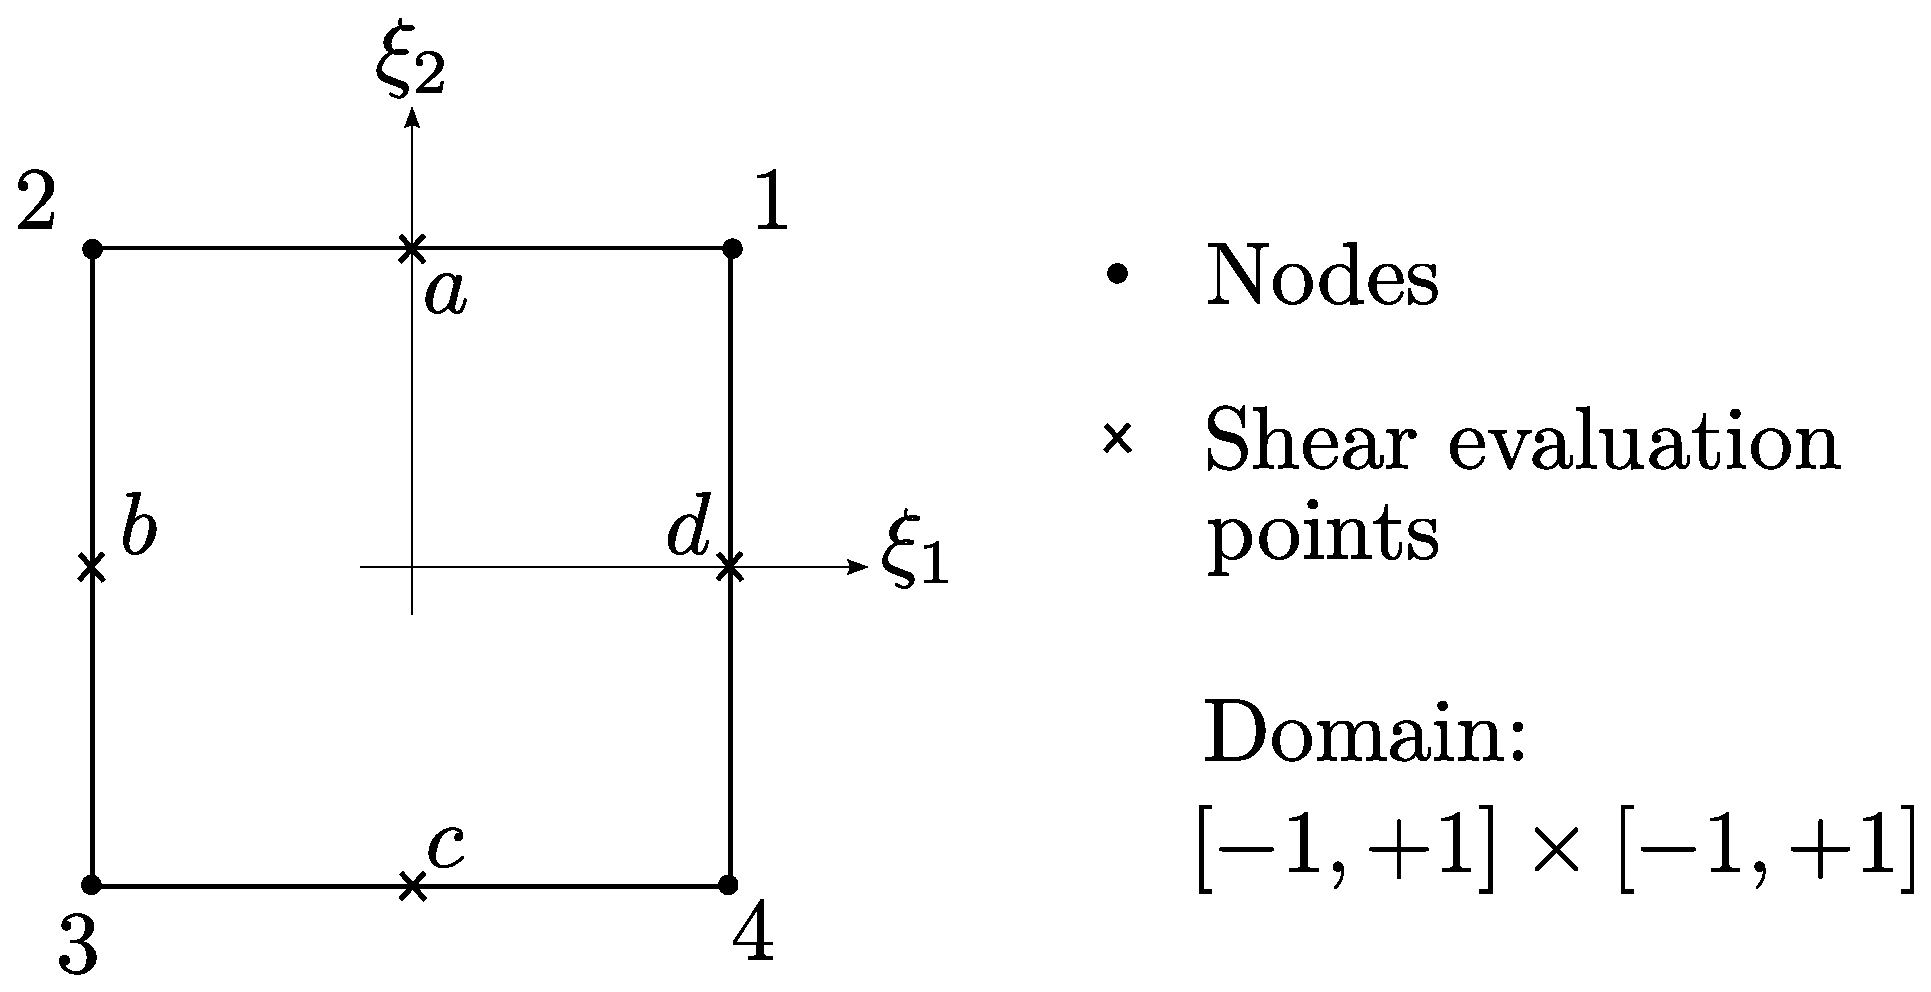
\includegraphics[width=.6\textwidth]{shellPic}
\caption{Shell: definitions}
\label{fig:EL:PLATE:SHELL4:sketch}
\end{figure}

Only linear elastic constitutive properties can be currently modeled.
They consist in a $12 \times 12$ matrix that expresses the force and moment
fluxes as functions of linear and angular strains according to
\begin{align}
	\cubr{\cvvect{
		n_{11} \\
		n_{12} \\
		n_{13} \\
		n_{21} \\
		n_{22} \\
		n_{23} \\
		m_{11} \\
		m_{12} \\
		m_{13} \\
		m_{21} \\
		m_{22} \\
		m_{23}
	}}
	&=
	\sqbr{D}
	\cubr{\cvvect{
		\varepsilon_{11} \\
		\varepsilon_{12} \\
		\varepsilon_{13} \\
		\varepsilon_{21} \\
		\varepsilon_{22} \\
		\varepsilon_{23} \\
		\kappa_{11} \\
		\kappa_{12} \\
		\kappa_{13} \\
		\kappa_{21} \\
		\kappa_{22} \\
		\kappa_{23}
	}}
	+
	\nt{prestress}
\end{align}
The \nt{prestress} is a force and moment per unit span contribution
to the force and moment fluxes.
Typically, only a membrane prestress makes sense, namely
\begin{Verbatim}[commandchars=\\\{\}]
    \bnt{prestress} ::= \bnt{T11} , \bnt{T12} , 0. , # force/span on face with normal 1
                    \bnt{T21} , \bnt{T22} , 0. , # force/span on face with normal 2
                    0.    , 0.    , 0. , # moment/span on face with normal 1
                    0.    , 0.    , 0.   # moment/span on face with normal 2
\end{Verbatim}
with $\nt{T21} \equiv \nt{T12}$.


When the \kw{isotropic} keyword is used, only two of the optional
sub-keywords \kw{E}, \kw{nu} and \kw{G} are required, as the remaining
parameter can be computed from the other two according to the relationship
\begin{align}
	\nt{G}
	&=
	\frac{\nt{E}}{2\plbr{1 + \nt{nu}}}
	.
\end{align}
If all are provided, they must be consistent.
The optional parameters \kw{as} and \kw{at} are not documented yet;
the default should be used.

When the (optional) \kw{matr} (or \kw{sym}) form is used,
the required data for an orthotropic plate, from Classical Laminate Theory (CLT),
with the principal axes of orthotropy parallel to the edges of the structure and laminate,
and with a symmetrical arrangement of the layers, are
\begin{align}
        \cubr{\cvvect{
                N_{x}
                \\
                N_{y}
                \\
                N_{xy}
                \\
                M_{x}
                \\
                M_{y}
                \\
                M_{xy}
        }}
        &=
        \sqbr{\matr{cccccc}{
	 CE_{x} & C\nu_{xy}E_y & 0 & 0 & 0 & 0 
	 \\
	 C\nu_{xy}E_y & CE_{y} & 0 & 0 & 0 & 0 
	 \\
	 0 & 0 & 2G_{xy}h & 0 & 0 & 0 
	 \\
	 0 & 0 & 0 & DE_{x} & D\nu_{xy}E_y & 0
	 \\
	 0 & 0 & 0 & D\nu_{xy}E_y & DE_{y} & 0 
	 \\
	 0 & 0 & 0 & 0 & 0 & 2F 
	        }}
        \cubr{\cvvect{
                \varepsilon_{x}
                \\
                \varepsilon_{y}
                \\
                \varepsilon_{xy}
                \\
                \kappa_{x}
		\\
                \kappa_{y}
		\\
                \kappa_{xy}
        }}
\end{align}
with
\begin{subequations}
\begin{align}
	C &= \frac{h}{1-\nu_{xy}\nu_{yx}}
	\\
	D &= \frac{h^3}{12(1-\nu_{xy}\nu_{yx})}
	\\
	F &= \frac{G_{xy}h^3}{12} 
\end{align}
\end{subequations}
The data actually required by MBDyn are
{\tiny
\begin{align}
        \cubr{\cvvect{
                N_{11}
                \\
                N_{12}
                \\
                N_{13}
                \\
                N_{21}
                \\
                N_{22}
                \\
                N_{23}
                \\
                M_{11}
                \\
                M_{12}
                \\
                M_{13}
		\\
                M_{21}
                \\
                M_{22}
                \\
                M_{23}
        }}
        &=
        \sqbr{\matr{cccccccccccc}{
  CE_{x} & 0      & 0      & 0 & C\nu_{xy}E_y & 0     & 0 & 0 & 0 & 0 & 0 & 0
  \\                                                                                
  0      & 2G_{xy}h  & 0   & 0 & 0  & 0               & 0 & 0 & 0 & 0 & 0 & 0
  \\                                                                             
  0      & 0      & \alpha_sG_{xy}h      & 0      & 0      & 0      & 0 & 0 & 0 & 0 & 0 & 0
  \\                                                                             
  0      & 0 & 0      & 2G_{xy}h & 0 & 0      & 0 & 0 & 0 & 0 & 0 & 0
  \\                                                                             
  C\nu_{xy}E_y & 0 & 0      & 0 & CE_{y} & 0      & 0 & 0 & 0 & 0 & 0 & 0
  \\                                                                             
  0      & 0      & 0      & 0      & 0      & \alpha_sG_{xy}h      & 0 & 0 & 0 & 0 & 0 & 0
  \\                                                                                                      
  0 & 0 & 0 & 0 & 0 & 0      & 2F & 0 & 0    & 0 & 0 & 0
  \\                                                                                                 
  0 & 0 & 0 & 0 & 0 & 0      & 0 & DE_x & 0    & -D\nu_{xy}E_y & 0 & 0
  \\                                                                                                 
  0 & 0 & 0 & 0 & 0 & 0      & 0      & 0        & 2F\alpha_t    & 0        & 0      & 0
  \\                                                                                                 
  0 & 0 & 0 & 0 & 0 & 0      & -D\nu_{xy}E_y & 0 & 0    & DE_y & 0 & 0
  \\                                                                                                 
  0 & 0 & 0 & 0 & 0 & 0      & 0 & 0 & 0    & 0 & 2F & 0
  \\                                                                                                 
  0 & 0 & 0 & 0 & 0 & 0      & 0      & 0        & 0    & 0        & 0      & 2F\alpha_t
        }}
        \cubr{\cvvect{
                \varepsilon_{11}
                \\
                \varepsilon_{12}
                \\
                \varepsilon_{13}
                \\
                \varepsilon_{21}
                \\
                \varepsilon_{22}
                \\
                \varepsilon_{23}
                \\
                \kappa_{11}
		\\
                \kappa_{12}
		\\
                \kappa_{13}
                \\
                \kappa_{21}
		\\
                \kappa_{22}
		\\
                \kappa_{23}
        }}
\end{align}
}

\noindent
where $\alpha_s$ is the shear factor, and the torsional factor $\alpha_t$ 
is the material coefficient typical for a 6-field shell theory, which does not appear in conventional shell theories.
It should be viewed as an analogue of the shear factor. 
Values of $\alpha_t$  from 0 to 1 have negligible influence on displacements and on the internal energy of the system.
See \cite{WITKOWSKI-2009-EAS-ANS} for details.

% \textbf{TODO: improve}



\subsection{Membrane4}
\label{sec:EL:PLATE:MEMBRANE4}

\emph{Authors: Marco Morandini and Tommaso Solcia}

The membrane4 element models a four-node membrane.
The syntax is
%\begin{verbatim}
\begin{Verbatim}[commandchars=\\\{\}]
    \bnt{elem_type} ::= \kw{membrane4eas} 

    \bnt{normal_arglist} ::=
        \bnt{node_1_label} , \bnt{node_2_label} , \bnt{node_3_label} , \bnt{node_4_label} ,
        \bnt{membrane_constitutive_law_data}

    \bnt{membrane_constitutive_law_data} ::=
        \{ [ \kw{matr} , ] \bnt{3x3_matrix}
            | \kw{sym} , \bnt{upper_triangular_3x3_matrix}
            | \kw{diag} , \bnt{diagonal_3x3_matrix}
            | \kw{isotropic} , \bnt{isotropic_data} \}
        [ , \kw{prestress} , (\hty{Vec3}) \bnt{prestress} ]

    \bnt{isotropic_data} ::=
        \{ \{ \kw{E} | \kw{Young modulus} \} , \bnt{E}
            | \{ \kw{nu} | \kw{Poisson modulus} \} , \bnt{nu}
            | \{ \kw{G} | \kw{shear modulus} \} , \bnt{G}
            | \kw{thickness} , \bnt{thickness} \}
        [ , ... ]
\end{Verbatim}
%\end{verbatim}
The name \kw{membrane4eas} stands for ``Enhanced Assumed Strain'' (EAS).
Nodes are numbered according to Figure~\ref{fig:EL:PLATE:SHELL4:sketch}.
Only linear elastic constitutive properties can be currently modeled.
They consist in a $3 \times 3$ matrix that expresses the force
fluxes as functions of linear strains according to
\begin{align}
	\cubr{\cvvect{
		n_{11} \\
		n_{22} \\
		n_{12}
	}}
	&=
	\sqbr{D}
	\cubr{\cvvect{
		\varepsilon_{11} \\
		\varepsilon_{22} \\
		\varepsilon_{12}
	}}
	+
	\nt{prestress}
\end{align}
The \nt{prestress} is a force per unit span contribution
to the force fluxes,
\begin{Verbatim}[commandchars=\\\{\}]
    \bnt{prestress} ::= \bnt{T11} , \bnt{T22} , \bnt{T12}
\end{Verbatim}

When the \kw{isotropic} keyword is used, only two of the optional
sub-keywords \kw{E}, \kw{nu} and \kw{G} are required, as the remaining
parameter can be computed from the other two according to the relationship
\begin{align}
	\nt{G}
	&=
	\frac{\nt{E}}{2\plbr{1 + \nt{nu}}}
	.
\end{align}
If all are provided, they must be consistent.


When the (optional) \kw{matr} (or \kw{sym}) form is used,
the required data for an orthotropic membrane are

\begin{align}
        \cubr{\cvvect{
                N_{11}
                \\
                N_{22}
                \\
                N_{12}
        }}
        &=
        \sqbr{\matr{cccccc}{
	 CE_{1} & C\nu_{21}E_1 & 0  
	 \\
	 C\nu_{12}E_2 & CE_{2} & 0  
	 \\
	 0 & 0 & 2G_{12}h  
       }}
        \cubr{\cvvect{
                \varepsilon_{11}
                \\
                \varepsilon_{22}
                \\
                \varepsilon_{12}
        }}
\end{align}
with
\begin{subequations}
\begin{align}
	C &= \frac{h}{1-\nu_{12}\nu_{21}}
	\\
	\nu_{12}E_2 &= \nu_{21}E_1 
\end{align}
\end{subequations}

\paragraph{Example:}
\begin{verbatim}
    membrane4eas: 100, 1, 2, 3, 4,
        matr, E1*H/(1-NU12*NU21),      E1*H*NU21/(1-NU12*NU21), 0,
              E2*NU12*H/(1-NU12*NU21), E2*H/(1-NU12*NU21),      0,
              0,                       0,                       2*G12*H,
        prestress, PS, PS, 0.;
\end{verbatim}





% Solid Elements
% MBDyn (C) is a multibody analysis code.
% http://www.mbdyn.org
%
% Copyright (C) 1996-2023
%
% Pierangelo Masarati  <pierangelo.masarati@polimi.it>
%
% Dipartimento di Ingegneria Aerospaziale - Politecnico di Milano
% via La Masa, 34 - 20156 Milano, Italy
% http://www.aero.polimi.it
%
% Changing this copyright notice is forbidden.
%
% This program is free software; you can redistribute it and/or modify
% it under the terms of the GNU General Public License as published by
% the Free Software Foundation (version 2 of the License).
%
%
% This program is distributed in the hope that it will be useful,
% but WITHOUT ANY WARRANTY; without even the implied warranty of
% MERCHANTABILITY or FITNESS FOR A PARTICULAR PURPOSE.  See the
% GNU General Public License for more details.
%
% You should have received a copy of the GNU General Public License
% along with this program; if not, write to the Free Software
% Foundation, Inc., 59 Temple Place, Suite 330, Boston, MA  02111-1307  USA

\section{Solid Elements}
\label{sec:EL:SOLID}
\emph{Author: Reinhard Resch}
\subsection{Scope}
In order to model general three dimensional solid structures with complex shape and subject to large deformations,
large strain and nonlinear material, a generic family of Isoparametric Finite Elements is implemented in MBDyn.
Those elements are based on a Total~Lagrangian~Formulation according to \cite{BATHE2016}.
Elements based on a pure displacement based formulation as well as a displacement/pressure formulation (u/p-c) are available.
Shape functions and integration points are based on \cite{BATHE2016}, \cite{DHONDT2004} and \cite{CODEASTERR30301}.
See also table~\ref{sec:EL:SOLID:elemtypes} and table~\ref{sec:EL:SOLID:elemtypes:upc} for a list of supported element types.
\subsection{Element input format}
\label{sec:EL:SOLID:INPUT:FORMAT}
\begin{Verbatim}[commandchars=\\\{\}]
  \bnt{elem_type} ::= \{ \kw{hexahedron8} | \kw{hexahedron20} | \kw{hexahedron20r} | \kw{hexahedron27} |
                    \kw{pentahedron15} | \kw{tetrahedron10} |
                    \kw{hexahedron8upc} | \kw{hexahedron20upc} | \kw{hexahedron20upcr} |
                    \kw{pentahedron15upc} | \kw{tetrahedron10upc} |
                    \kw{hexahedron8f} | \kw{hexahedron20f} | \kw{hexahedron20fr} | \kw{hexahedron27f} |
                    \kw{pentahedron15f} | \kw{tetrahedron10f} \}

    \bnt{normal_arglist} ::=
        [ \kw{static} , ] [ \kw{lumped mass} , ] \bnt{struct_node_data}, [ \bnt{hydr_node_data}, ]
        \bnt{nodal_density}, \bnt{constitutive_law_data} ;

     \bnt{struct_node_data} :: =
        (\ty{StructDispNode}) \bnt{struct_node_1_label} ,
        (\ty{StructDispNode}) \bnt{struct_node_2_label} ,
        ... ,
        (\ty{StructDispNode}) \bnt{struct_node_N_label}


     \bnt{hydr_node_data} :: =
        (\ty{HydraulicNode}) \bnt{hydr_node_1_label} ,
        (\ty{HydraulicNode}) \bnt{hydr_node_2_label} ,
        ... ,
        (\ty{HydraulicNode}) \bnt{hydr_node_N_label}

     \bnt{nodal_density} :: =
        (\ty{real}) \bnt{rho_1}, (\ty{real}) \bnt{rho_2} , ... , (\ty{real}) \bnt{rho_N}

     \bnt{constitutive_law_data} :: =
        \{ \bnt{constitutive_law_data_6D} | \bnt{constitutive_law_data_7D} | \bnt{constitutive_law_data_9D} \}

      \bnt{constitutive_law_data_6D} :: =
        (\htybkw{ConstitutiveLaw}{6D}) \bnt{constitutive_law_1} ,
        \{ (\htybkw{ConstitutiveLaw}{6D}) \bnt{constitutive_law_2} | \kw{same} \} ,
        ... ,
        \{ (\htybkw{ConstitutiveLaw}{6D}) \bnt{constitutive_law_M} | \kw{same} \}

      \bnt{constitutive_law_data_7D} :: =
        (\htybkw{ConstitutiveLaw}{7D}) \bnt{constitutive_law_1} ,
        \{ (\htybkw{ConstitutiveLaw}{7D}) \bnt{constitutive_law_2} | \kw{same} \} ,
        ... ,
        \{ (\htybkw{ConstitutiveLaw}{7D}) \bnt{constitutive_law_M} | \kw{same} \}

      \bnt{constitutive_law_data_9D} :: =
        (\htybkw{ConstitutiveLaw}{9D}) \bnt{constitutive_law_1} ,
        \{ (\htybkw{ConstitutiveLaw}{9D}) \bnt{constitutive_law_2} | \kw{same} \} ,
        ... ,
        \{ (\htybkw{ConstitutiveLaw}{9D}) \bnt{constitutive_law_M} | \kw{same} \}
\end{Verbatim}

\subsection{Constitutive law types to be used for solid elements}
Each solid element type described in section~\ref{sec:EL:SOLID:INPUT:FORMAT} has a dedicated type of constitutive law which must be used.
See table~\ref{SEC:EL:ELEMTYPE:CONSTLAW}.
\begin{table}[h!tp]
  \begin{tabular}[t]{|l|c|c|c|}
  \hline
               & \multicolumn{3}{|c|}{constitutive law} \tabularnewline
  \hline
  element type & 6D & 7D & 9D \tabularnewline
  \hline
  \kw{hexahedron8} & $\surd$ & & \tabularnewline
  \hline
  \kw{hexahedron20} & $\surd$ & & \tabularnewline
  \hline
  \kw{hexahedron20r} & $\surd$ & & \tabularnewline
  \hline
  \kw{hexahedron27} & $\surd$ & & \tabularnewline
  \hline
  \kw{pentahedron15} & $\surd$ & & \tabularnewline
  \hline
  \kw{tetrahedron10} & $\surd$ & & \tabularnewline
  \hline
  \kw{hexahedron8upc} & & $\surd$ & \tabularnewline
  \hline
  \kw{hexahedron20upc} & & $\surd$ & \tabularnewline
  \hline
  \kw{hexahedron20upcr} & & $\surd$ & \tabularnewline
  \hline
  \kw{pentahedron15upc} & & $\surd$ & \tabularnewline
  \hline
  \kw{tetrahedron10upc} & & $\surd$ & \tabularnewline
  \hline
  \kw{hexahedron8f} & & & $\surd$ \tabularnewline
  \hline
  \kw{hexahedron20f} & & & $\surd$ \tabularnewline
  \hline
  \kw{hexahedron20fr} & & & $\surd$ \tabularnewline
  \hline
  \kw{hexahedron27f} & & & $\surd$ \tabularnewline
  \hline
  \kw{pentahedron15f} & & & $\surd$ \tabularnewline
  \hline
  \kw{tetrahedron10f} & & & $\surd$ \tabularnewline
  \hline
  \end{tabular}
  \caption{Constitutive laws to be used for each solid element type}
  \label{SEC:EL:ELEMTYPE:CONSTLAW}
\end{table}

\subsection{Displacement based elements versus displacement/pressure elements (u/p-c)}
All pure displacement based elements (e.g. \kw{hexahedron8}, \ldots) require only structural displacement nodes,
whereas displacement/pressure based elements (e.g. \kw{hexahedron8upc}, \ldots) require
additional hydraulic nodes, in order to represent the hydrostatic pressure.
Usually the number of hydraulic nodes is lower than the number of structural nodes in order to prevent
locking phenomenon \cite{BATHE2016}.
Due to the use of dedicated hydraulic nodes, the hydrostatic portion of the stress tensor is always continuous
across compatible elements with common nodes \cite{BATHE2016}. For that reason, those elements have the
suffix~*-\kw{upc} in their element names, which stands for displacement/pressure-continuous (u/p-c).
In addition to that, even fully incompressible constitutive laws like Mooney Rivlin are supported
by u/p-c~elements \cite{BATHE2016}.

\subsection{Dynamic versus static elements}
By default, dynamic solid elements with inertia effects enabled are created,
unless the keyword \kw{static} is used in the element description
or the statement ``\kw{model}: \kw{static}'' was present inside the control data block according section~\ref{sec:CONTROLDATA:MODEL}.
\subsection{Gravity and rigid body kinematics}
All solid elements including static ones, are supporting gravity loads according section~\ref{sec:ELEMENTS:gravity}
and rigid body kinematics according section~\ref{sec:CONTROLDATA:RBK}.
\subsection{Material properties and constitutive laws}
For that reason, the density of the material must be provided also for static solid elements.
Solid elements may have variable density within a single element.
Also in case of constant density, density values must be provided for each node, and it will be interpolated between nodes.
Any linear or nonlinear elastic or viscoelastic constitutive law can be used, if it fulfills the following requirements:
A constitutive law must expect the components $\boldsymbol{\varepsilon}$ of the Green-Lagrange strain tensor $\boldsymbol{G}$,
and optionally it's scaled time derivatives $\dot{\boldsymbol{\varepsilon}}^{\star}$ as input, and return the components $\boldsymbol{\sigma}$
of the Second~Piola-Kirchhoff stress tensor $\boldsymbol{S}$ as output. The following types of constitutive laws are implemented:
\begin{itemize}
\item linear elastic isotropic
\item linear viscoelastic isotropic,
\item hyperelastic isotropic
\item elasto-plastic with isotropic hardening
\item generalized Maxwell~viscoelastic
\item constitutive laws provided by the \href{thelfer.github.io/tfel/web/index.html}{MFront} code generation tool
\end{itemize}
See also section~\ref{sec:CL:hookean:linear:elastic:isotropic}, section~\ref{sec:CL:neo-hookean}, section~\ref{sec:CL:mooney-rivlin},
section~\ref{sec:CL:bilinear-isotropic-hardening}, section~\ref{sec:CL:linear-viscoelastic-maxwell} and section~\ref{sec:CL:mfront}.
In case of viscoelastic constitutive laws, the strain rates $\dot{\boldsymbol{\varepsilon}}$ are scaled in order to make
the effect of structural damping independent on the strain \cite{KUEBLER2005}.

\begin{eqnarray}
  \label{sec:EL:SOLID:constlaw}
  \boldsymbol{\sigma} & = & \boldsymbol{f}\left(\boldsymbol{\varepsilon},\, \dot{\boldsymbol{\varepsilon}}^{\star}\right) \\
  \boldsymbol{\sigma} & = & \begin{pmatrix} S_{11} & S_{22} & S_{33} & S_{12} & S_{23} & S_{31} \end{pmatrix}^T \\
  \boldsymbol{\varepsilon} & = & \begin{pmatrix} G_{11} & G_{22} & G_{33} & 2\,G_{12} & 2\,G_{23} & 2\,G_{31} \end{pmatrix}^T \\
  \dot{\boldsymbol{\varepsilon}}^{\star} & = & \begin{pmatrix} \dot{G}_{11}^{\star} & \dot{G}_{22}^{\star} & \dot{G}_{33}^{\star} & 2\,\dot{G}_{12}^{\star} & 2\,\dot{G}_{23}^{\star} & 2\,\dot{G}_{31}^{\star} \end{pmatrix}^T \\
  \dot{\boldsymbol{G}}^{\star} & = & \boldsymbol{C}^{-1} \, \dot{\boldsymbol{G}} \, \boldsymbol{C}^{-1} \, \det{\boldsymbol{F}} \\
  \boldsymbol{G} & = & \frac{1}{2}\,\left(\boldsymbol{C} - \boldsymbol{I}\right) \\
  \boldsymbol{C} & = & \boldsymbol{F}^T\,\boldsymbol{F} \\
  \boldsymbol{F} & = & \nabla \boldsymbol{u} + \boldsymbol{I}
\end{eqnarray}
\begin{description}
\item[$\boldsymbol{f}$] Constitutive law
\item[$\boldsymbol{G}$] Green-Lagrange strain tensor
\item[$\boldsymbol{S}$] Second~Piola-Kirchhoff stress tensor
\item[$\boldsymbol{C}$] Right~Cauchy-Green strain tensor
\item[$\boldsymbol{F}$] Deformation gradient
\item[$\boldsymbol{u}$] Deformation field
\end{description}

\paragraph{Constitutive laws for incompressible materials}
All Finite Elements based on a pure displacement based formulation (e.g. \kw{hexahedron8}, \ldots) require 6D constitutive laws,
whereas elements based on a displacement/pressure (u/p-c) formulation (e.g. \kw{hexahedron8upc}, \ldots) require 7D constitutive laws.
In the latter case, the additional component of the strain tensor $\boldsymbol{\varepsilon}_7$ is used to pass the interpolated
hydrostatic pressure $\tilde{p}$, and the additional component of the stress tensor $\boldsymbol{\sigma}_7$ is used to return an
expression related to the condition of volumetric compatibility. See equations~\ref{SEC:EL:solid:constlaw:upc:eps} to \ref{SEC:EL:solid:constlaw:upc:epsV}.
\begin{eqnarray}
  \boldsymbol{\sigma} & = & \begin{pmatrix} S_{11} & S_{22} & S_{33} & S_{12} & S_{23} & S_{31} & \frac{1}{\kappa}\left(\bar{p} - \tilde{p}\right) \end{pmatrix}^T \label{SEC:EL:solid:constlaw:upc:eps} \\
  \boldsymbol{\varepsilon} & = & \begin{pmatrix} G_{11} & G_{22} & G_{33} & 2\,G_{12} & 2\,G_{23} & 2\,G_{31} & \tilde{p} \end{pmatrix}^T \label{SEC:EL:solid:constlaw:upc:sigma}
\end{eqnarray}
For isotropic materials, the condition of volumetric compatibility is \cite{BATHE2016}.
\begin{equation}
\int_{V}\frac{1}{\kappa}\left(\bar{p} - \tilde{p}\right)\,\frac{\partial\tilde{p}}{\partial\hat{p}_i}\,dV = 0 \label{SEC:EL:solid:constlaw:upc:epsV}
\end{equation}
\begin{description}
\item[$\bar{p}$] Hydrostatic pressure calculated from the strain tensor $\boldsymbol{G}$
\item[$\tilde{p}$] Hydrostatic pressure interpolated from the hydraulic nodes of the element
\item[$\hat{p}$] Hydrostatic pressure at the hydraulic nodes of the element
\item[$\kappa$] Bulk modulus (e.g. $\kappa=\frac{E}{3\,\left(1-2\nu\right)}$ for linear elastic isotropic materials)
\end{description}

\paragraph{Constitutive laws based on the deformation gradient and the First~Piola-Kirchhoff stress tensor}
\label{sec:EL:SOLID:constlaw:F}
For a few constitutive laws (e.g. \kw{mfront finite strain}), it is necessary to provide
the unsymmetric deformation gradient $\boldsymbol{F}$ as input value instead of the symmetric
Green~Lagrange strain tensor $\boldsymbol{G}$.
As a consequence, it is necessary to use a \htybkw{ConstitutiveLaw}{9D} in order to pass all nine components of the unsymmetric $3 \times 3$ tensor $\boldsymbol{F}$.
\subparagraph{Conventions}
Since this type of constitutive law was intended mainly to provide support for a constitutive law called \kw{mfront finite strain},
the conventions of the \href{https://thelfer.github.io/mgis/web/index.html}{MFrontGenericInterfaceSupport} library are applied\cite{helfer_introducing_2015}. See also section~\ref{sec:CL:mfront}.
\begin{eqnarray}
  \boldsymbol{\sigma} & = & \begin{pmatrix} P_{11} & P_{22} & P_{33} & P_{12} & P_{21} & P_{13} & P_{31} & P_{23} & P_{32} \end{pmatrix}^T \\
  \boldsymbol{\varepsilon} & = & \begin{pmatrix} F_{11} & F_{22} & F_{33} & F_{12} & F_{21} & F_{13} & F_{31} & F_{23} & F_{32} \end{pmatrix}^T \\
  \boldsymbol{P} & = & \boldsymbol{F} \, \boldsymbol{S}
\end{eqnarray}
\begin{description}
\item[$\boldsymbol{P}$] First~Piola-Kirchhoff stress tensor
\end{description}

\paragraph{Constitutive laws and integration points}
One constitutive law must be provided per integration point.
As a consequence it is possible to build elements with varying elastic properties across a single element.
The actual number of integration points is shown in table~\ref{sec:EL:SOLID:elemtypes} and table~\ref{sec:EL:SOLID:elemtypes:upc}.
\subsection{Output}
\paragraph{Output of stress and strain}
By default six components of the Cauchy stress tensor $\bar{\boldsymbol{\tau}}$ and six strains $\bar{\boldsymbol{\varepsilon}}$ at element nodes are written to the output file.
See also equation~\ref{SEC:EL:solid:output:start} to equation~\ref{SEC:EL:solid:output:end} which are based on \cite{WALLRAPP1998}.
Since stress and strain are evaluated at integration points instead of nodes, it is required to extrapolate $\bar{\boldsymbol{\tau}}$ and $\bar{\boldsymbol{\varepsilon}}$
from integration points to nodes using Lapack's DGELSD function.
\begin{eqnarray}
  \boldsymbol{\tau} & = & \frac{1}{\det{\boldsymbol{F}}} \, \boldsymbol{F} \, \boldsymbol{S} \, \boldsymbol{F}^T   \label{SEC:EL:solid:output:start} \\
  \bar{\varepsilon}_{\alpha} & = & \sqrt{C_{\alpha\alpha}} - 1 \\
  \sin{\vartheta_{\alpha\beta}} & = & \frac{C_{\alpha\beta}}{\left(1 + \bar{\varepsilon}_{\alpha}\right)\left(1 + \bar{\varepsilon}_{\beta}\right)}   \label{SEC:EL:solid:output:end}  \\
  \bar{\boldsymbol{\tau}} & = & \begin{pmatrix}
    \tau_{11} &
    \tau_{22} &
    \tau_{33} &
    \tau_{12} &
    \tau_{23} &
    \tau_{31}
  \end{pmatrix}^T \\
  \bar{\boldsymbol{\varepsilon}} & = & \begin{pmatrix}
    \bar{\varepsilon}_1 &
    \bar{\varepsilon}_2 &
    \bar{\varepsilon}_3 &
    \sin{\vartheta}_{12} &
    \sin{\vartheta}_{23} &
    \sin{\vartheta}_{31}
  \end{pmatrix}^T
\end{eqnarray}

\paragraph{Output of accelerations}
By default dynamic solid elements are using a consistent mass matrix. In order to enable output of accelerations
for dynamic structural nodes, it is required to use a lumped mass matrix.
For that purpose the keyword \kw{lumped mass} must be used.
Due to the special handling of accelerations in MBDyn, only solid elements with lumped mass matrix enabled
can be used to compute accelerations for structural nodes as described in section~\ref{sec:NODE:STRUCTURAL:SYNTAX:accel}.

\begin{table}[h!tp]
\begin{tabular}[t]{|l|c|c|c|c|c|c|c|}
  \hline
  element type & nodes & node order & integration points & order & integration  & references \tabularnewline
  \hline
  \kw{hexahedron8} & 8 & \ref{fig:EL:SOLID:HEXAHEDRON8} & 8 & 1 & full & \cite{BATHE2016} \tabularnewline
  \hline
  \kw{hexahedron20} & 20 & \ref{fig:EL:SOLID:HEXAHEDRON20} & 27 & 2 & full & \cite{BATHE2016} \tabularnewline
  \hline
  \kw{hexahedron20r} & 20 & \ref{fig:EL:SOLID:HEXAHEDRON20R} & 8 & 2 & reduced & \cite{DHONDT2004} \tabularnewline
  \hline
  \kw{hexahedron27} & 27 & \ref{fig:EL:SOLID:HEXAHEDRON27} & 27 & 2 & full & \cite{CODEASTERR30301} \tabularnewline
  \hline
  \kw{pentahedron15} & 15 & \ref{fig:EL:SOLID:PENTAHEDRON15} & 21 & 2 & full & \cite{CODEASTERR30301} \tabularnewline
  \hline
  \kw{tetrahedron10} & 10 & \ref{fig:EL:SOLID:TETRAHEDRON10H} & 5 & 2 & full & \cite{CODEASTERR30301} \tabularnewline
  \hline
\end{tabular}
\caption{Finite Element Types using a pure displacement based formulation}
\label{sec:EL:SOLID:elemtypes}
\end{table}

\begin{table}[h!tp]
\begin{tabular}[t]{|l|c|c|c|c|c|c|c|c|}
  \hline
  element type & nodes-u & node order-u & nodes-p & integration points & order & integration & references \tabularnewline
  \hline
  \kw{hexahedron8upc} & 8 & \ref{fig:EL:SOLID:HEXAHEDRON8} & 1 & 8 & 1 & full & \cite{BATHE2016} \tabularnewline
  \hline
  \kw{hexahedron20upc} & 20 & \ref{fig:EL:SOLID:HEXAHEDRON20} & 8 & 27 & 2 & full & \cite{BATHE2016} \tabularnewline
  \hline
  \kw{hexahedron20upcr} & 20 & \ref{fig:EL:SOLID:HEXAHEDRON20R} & 8 & 8 & 2 & reduced & \cite{DHONDT2004} \tabularnewline
  \hline
  \kw{pentahedron15upc} & 15 & \ref{fig:EL:SOLID:PENTAHEDRON15} & 6 & 21 & 2 & full & \cite{CODEASTERR30301} \tabularnewline
  \hline
  \kw{tetrahedron10upc} & 10 & \ref{fig:EL:SOLID:TETRAHEDRON10H} & 4 & 5 & 2 & full & \cite{CODEASTERR30301} \tabularnewline
  \hline
\end{tabular}
\caption{Finite Element Types using a displacement/pressure formulation}
\label{sec:EL:SOLID:elemtypes:upc}
\end{table}

\begin{table}[h!tp]
\begin{tabular}[t]{|l|c|c|c|c|c|c|c|c|}
  \hline
  element type & nodes-u & node order-u  & integration points & order & integration & references \tabularnewline
  \hline
  \kw{hexahedron8f} & 8 & \ref{fig:EL:SOLID:HEXAHEDRON8}  & 8 & 1 & full & \cite{BATHE2016} \tabularnewline
  \hline
  \kw{hexahedron20f} & 20 & \ref{fig:EL:SOLID:HEXAHEDRON20} & 27 & 2 & full & \cite{BATHE2016} \tabularnewline
  \hline
  \kw{hexahedron20fr} & 20 & \ref{fig:EL:SOLID:HEXAHEDRON20R} & 8 & 2 & reduced & \cite{DHONDT2004} \tabularnewline
  \hline
  \kw{pentahedron15f} & 15 & \ref{fig:EL:SOLID:PENTAHEDRON15} & 21 & 2 & full & \cite{CODEASTERR30301} \tabularnewline
  \hline
  \kw{tetrahedron10f} & 10 & \ref{fig:EL:SOLID:TETRAHEDRON10H} & 5 & 2 & full & \cite{CODEASTERR30301} \tabularnewline
  \hline
\end{tabular}
\caption{Finite Element Types using the deformation gradient and the First~Piola-Kirchhoff stress tensor}
\label{sec:EL:SOLID:elemtypes:F}
\end{table}

\paragraph{Private Data}
\label{sec:EL:SOLID:PRIVATE}
The following private data is available:
\begin{enumerate}
\item \kw{"E"} Kinetic energy
\end{enumerate}
Kinetic energy is always zero if the keyword \kw{static} was used or if the statement
``\kw{model}: \kw{static}'' was present inside the control data block according
section~\ref{sec:CONTROLDATA:MODEL}.

\begin{figure}[htb]
  \begin{subfigure}{0.5\textwidth}
    \centering
    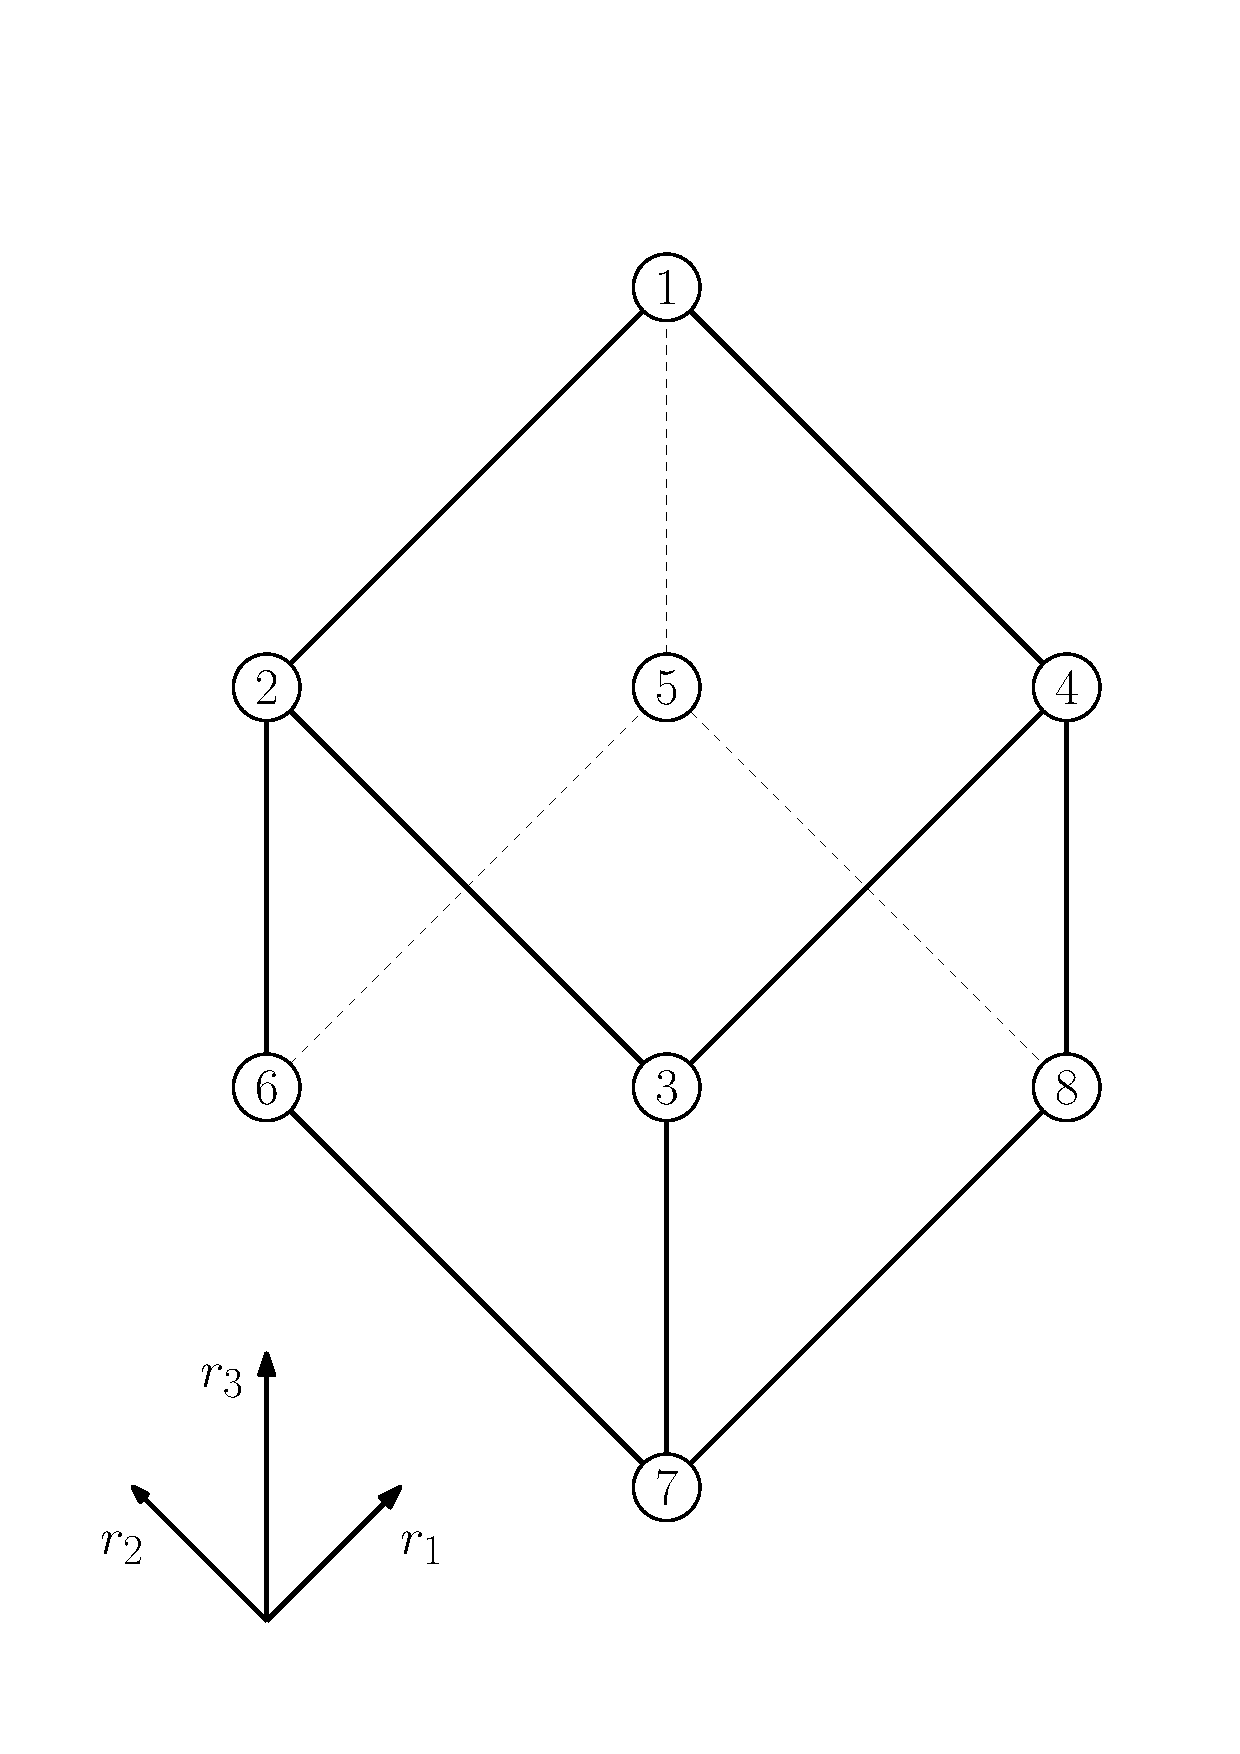
\includegraphics[width=.5\textwidth]{hexahedron8}
    \caption{hexahedron8}
    \label{fig:EL:SOLID:HEXAHEDRON8}
  \end{subfigure}
  \begin{subfigure}{0.5\textwidth}
    \centering
    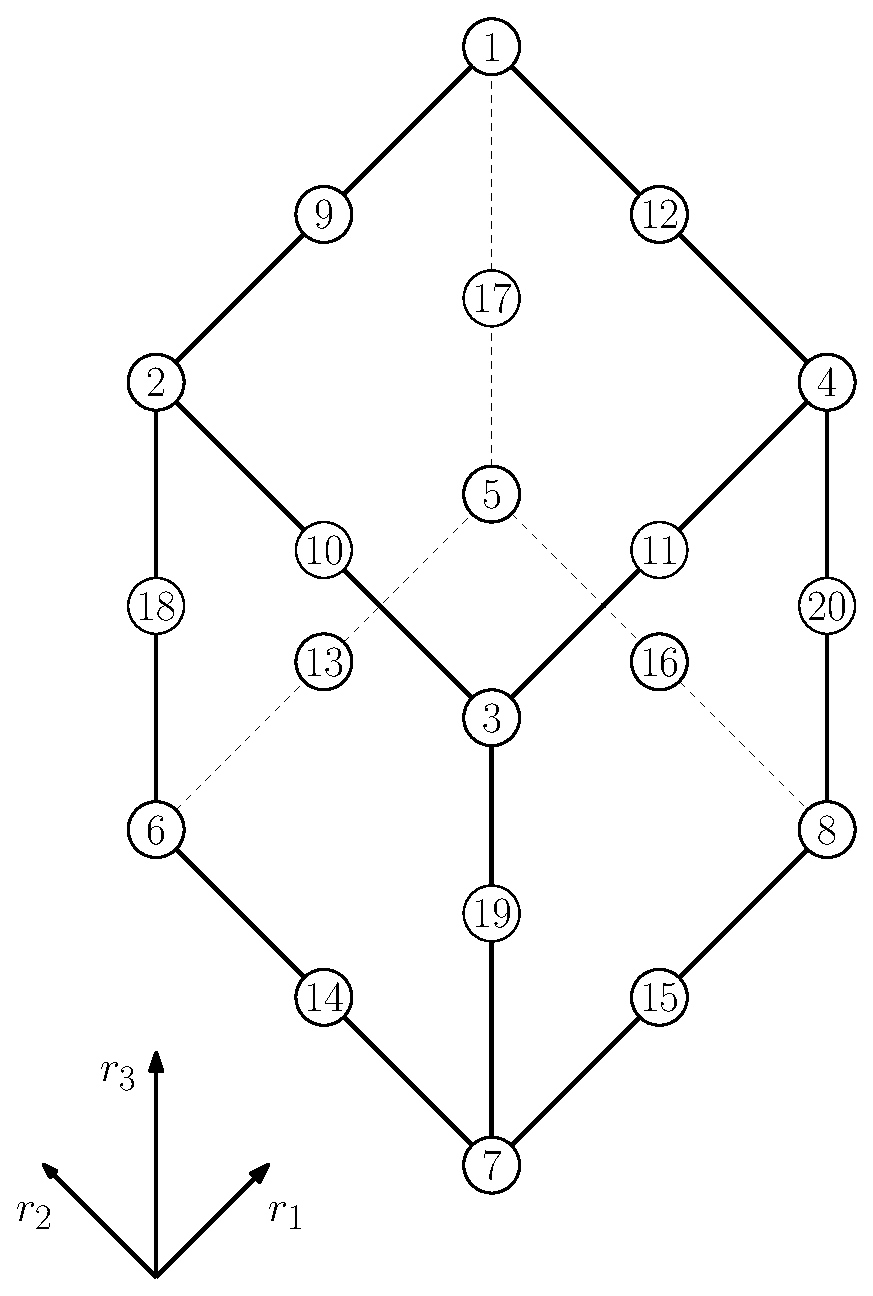
\includegraphics[width=.5\textwidth]{hexahedron20}
    \caption{hexahedron20}
    \label{fig:EL:SOLID:HEXAHEDRON20}
  \end{subfigure}
  \begin{subfigure}{0.5\textwidth}
    \centering
    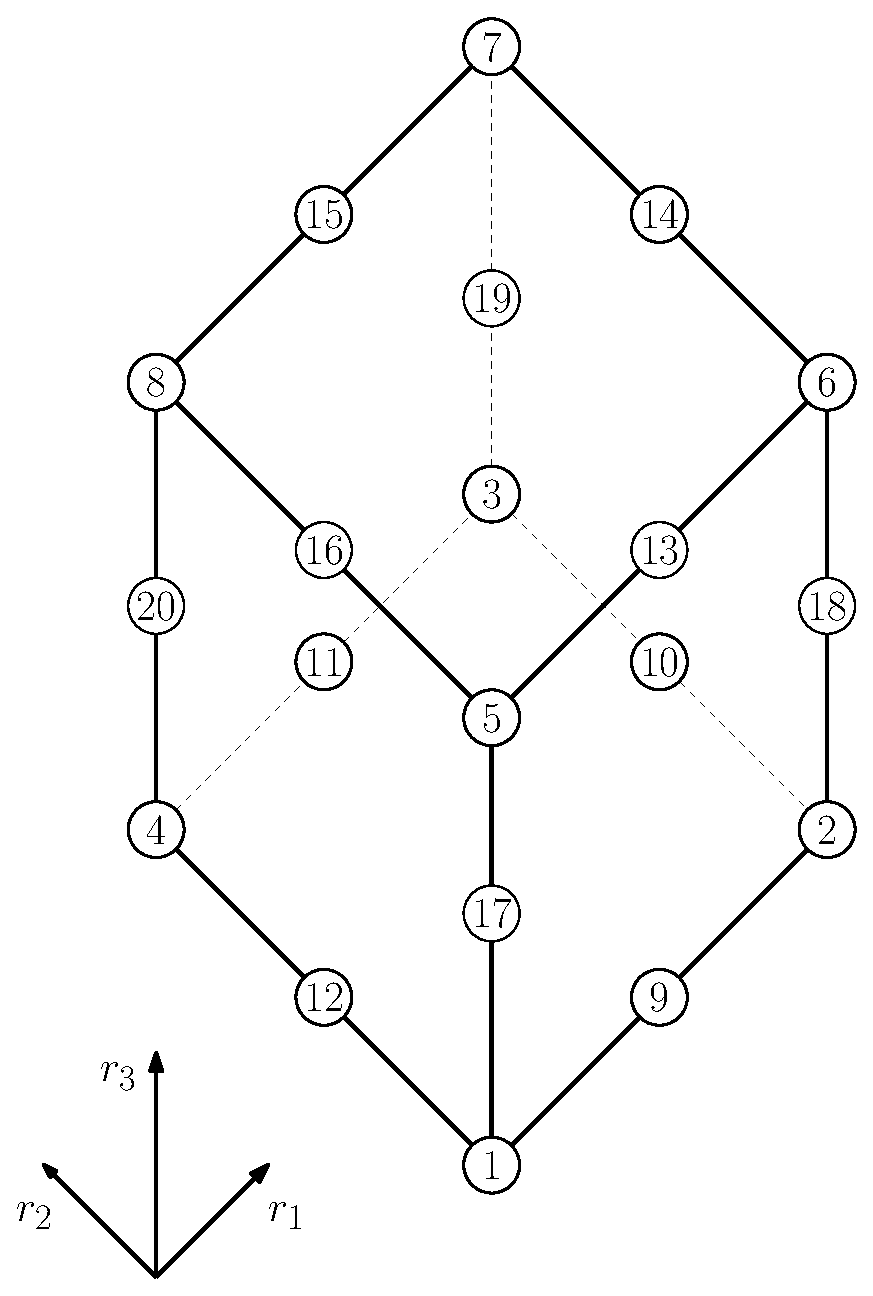
\includegraphics[width=.5\textwidth]{hexahedron20r}
    \caption{hexahedron20r}
    \label{fig:EL:SOLID:HEXAHEDRON20R}
  \end{subfigure}
  \begin{subfigure}{0.5\textwidth}
    \centering
    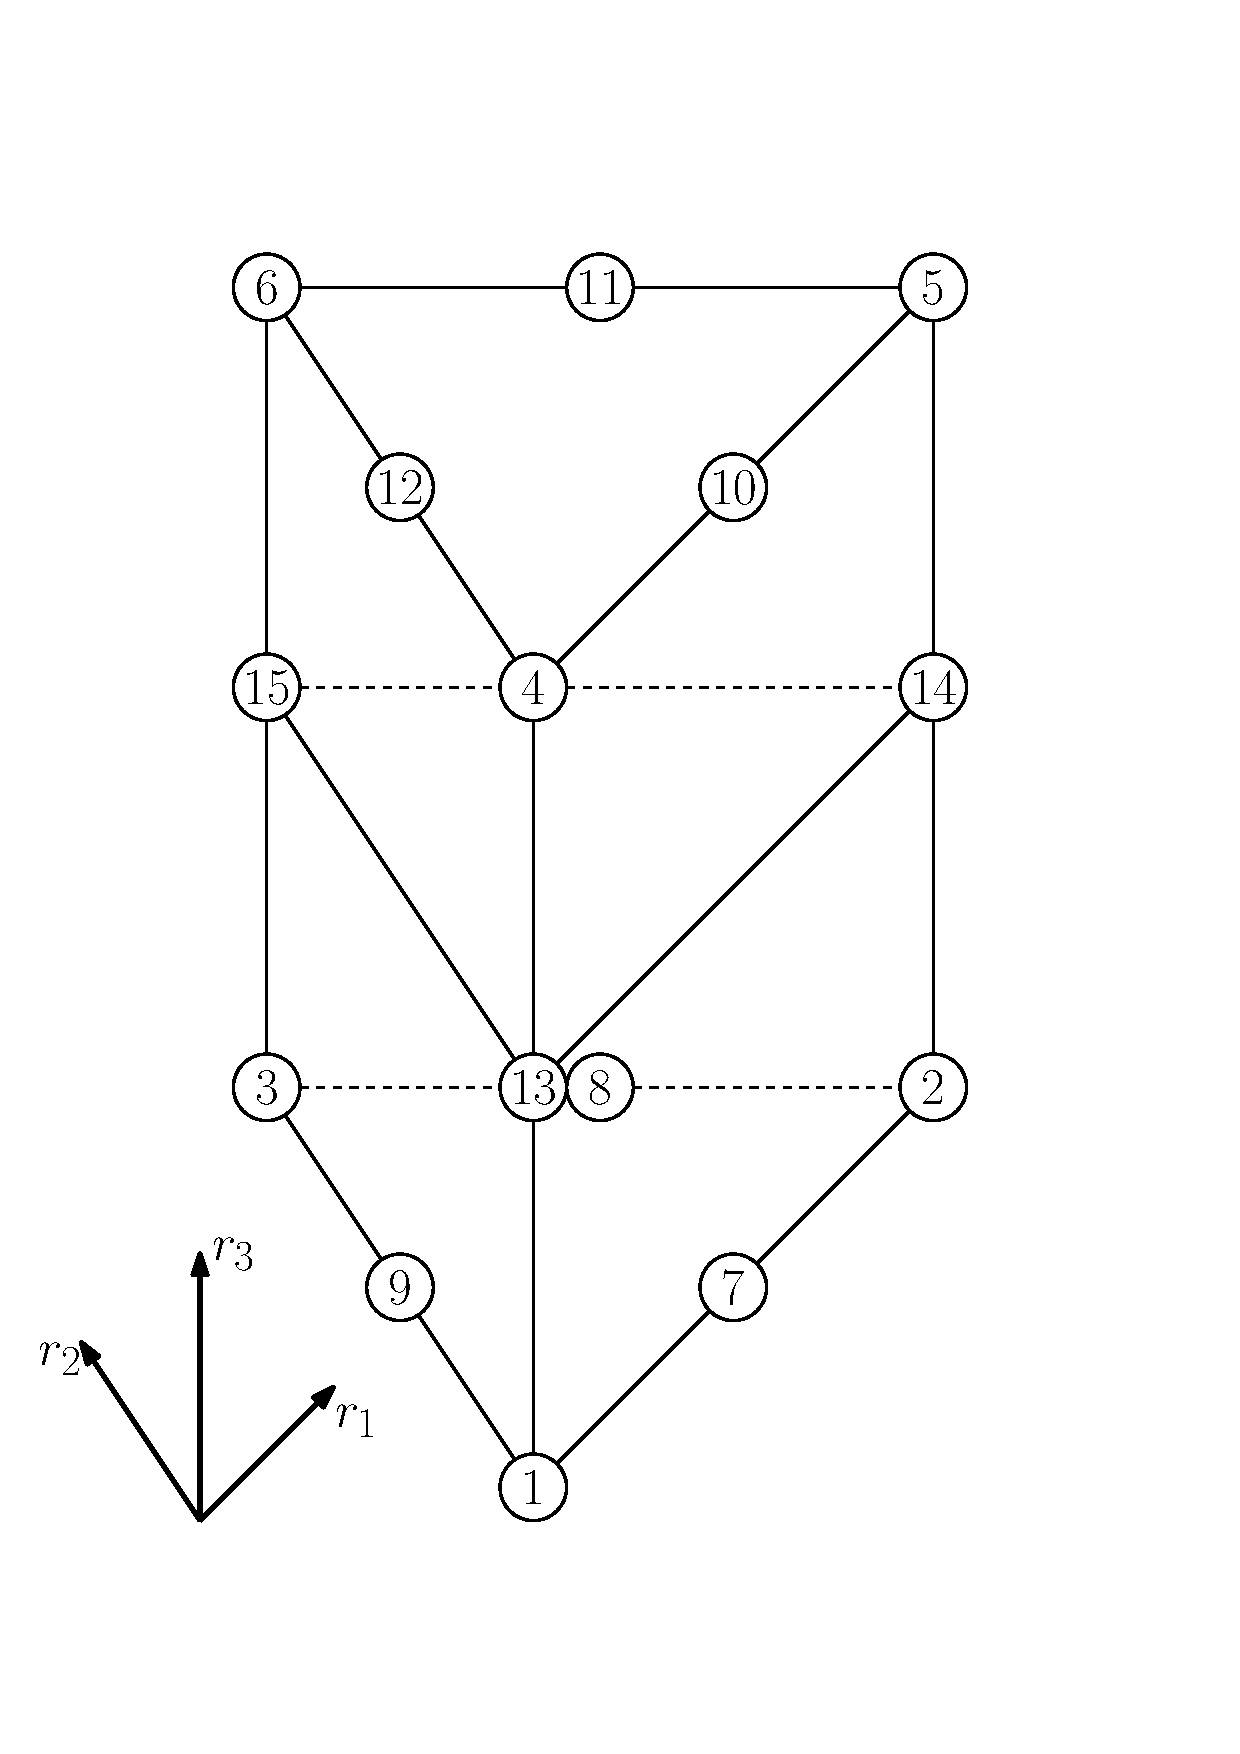
\includegraphics[width=.5\textwidth]{pentahedron15}
    \caption{pentahedron15}
    \label{fig:EL:SOLID:PENTAHEDRON15}
  \end{subfigure}
  \begin{subfigure}{0.5\textwidth}
    \centering
    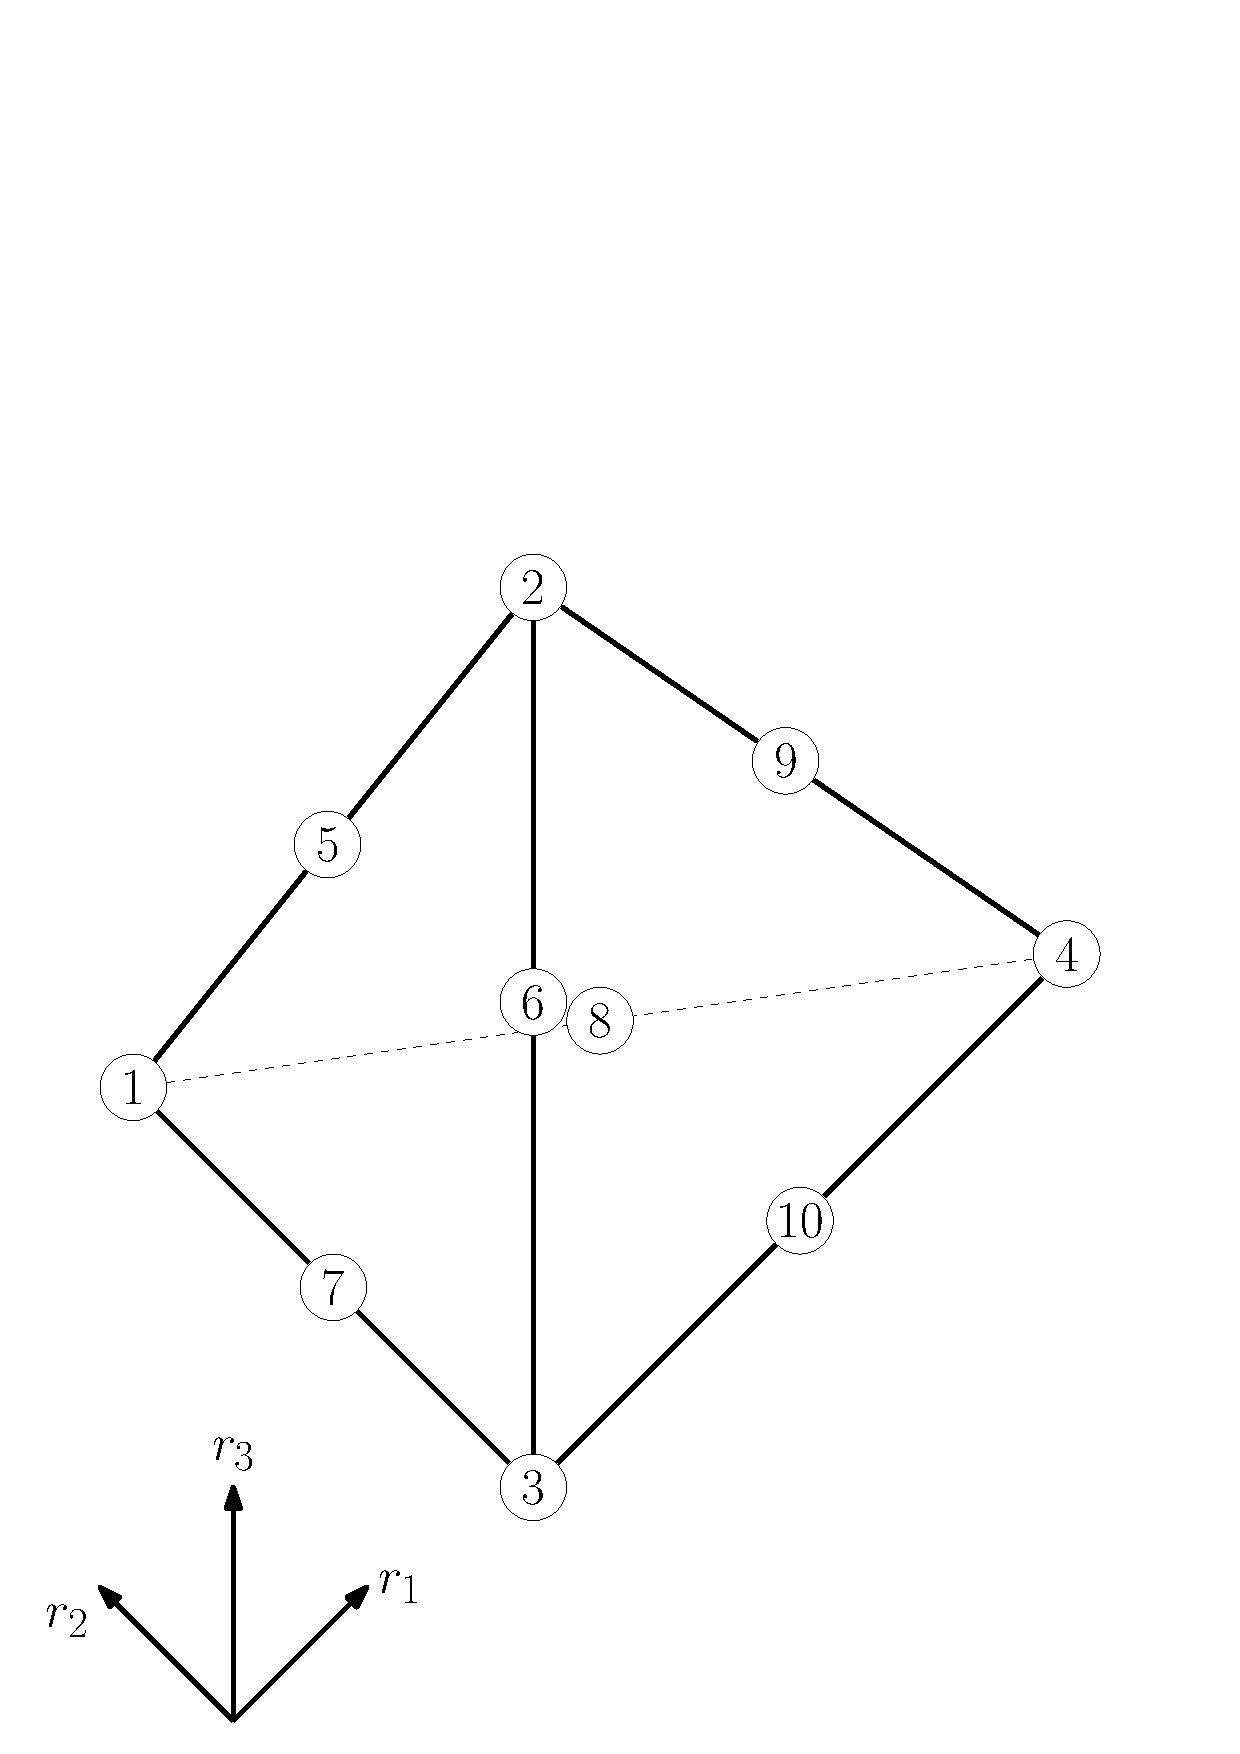
\includegraphics[width=.5\textwidth]{tetrahedron10h}
    \caption{tetrahedron10}
    \label{fig:EL:SOLID:TETRAHEDRON10H}
  \end{subfigure}
  \caption{Node order}
  \label{fig:EL:SOLID:NODE_ORDER}
\end{figure}

\begin{figure}[htb]
\centering
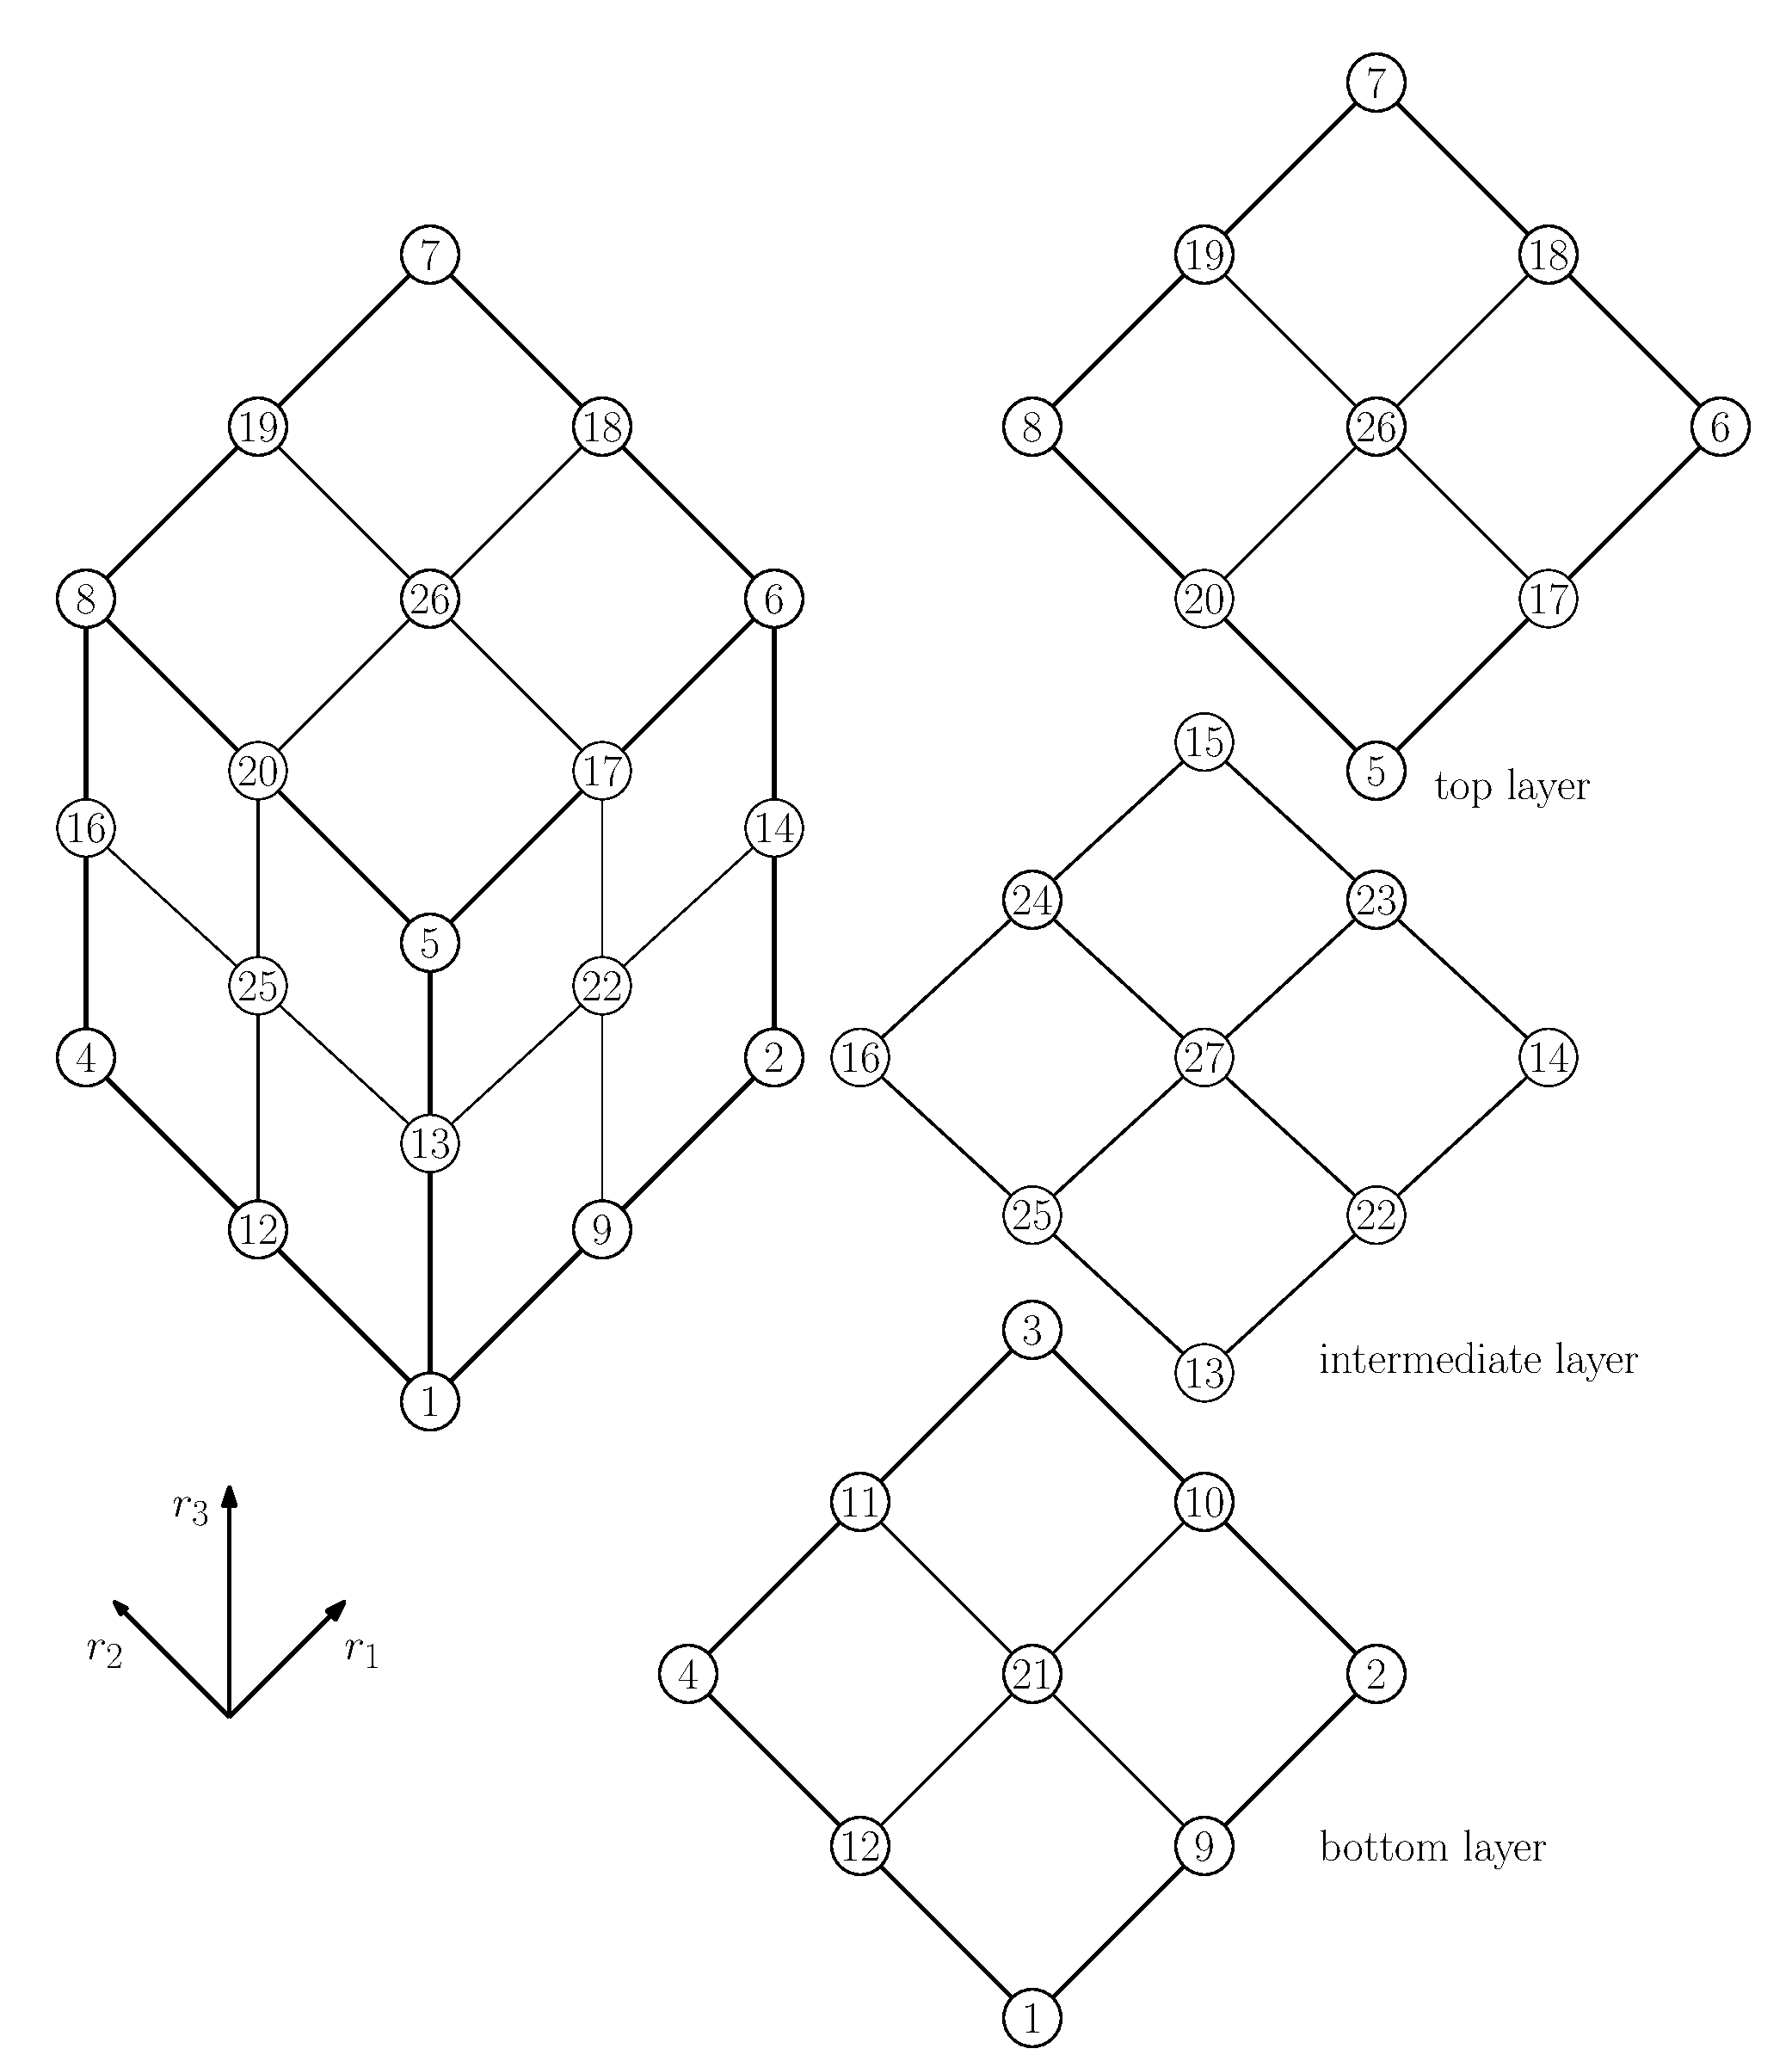
\includegraphics[width=.5\textwidth]{hexahedron27}
\caption{Node order: hexahedron27}
\label{fig:EL:SOLID:HEXAHEDRON27}
\end{figure}

\subsection{Example:}
\begin{verbatim}
    constitutive law: 1, name, "solid1", 6,
             linear viscoelastic generic,
             matr , 2.82e+11, 1.21e+11, 1.21e+11, 0.00e+00, 0.00e+00, 0.00e+00,
                    1.21e+11, 2.82e+11, 1.21e+11, 0.00e+00, 0.00e+00, 0.00e+00,
                    1.21e+11, 1.21e+11, 2.82e+11, 0.00e+00, 0.00e+00, 0.00e+00,
                    0.00e+00, 0.00e+00, 0.00e+00, 8.07e+10, 0.00e+00, 0.00e+00,
                    0.00e+00, 0.00e+00, 0.00e+00, 0.00e+00, 8.07e+10, 0.00e+00,
                    0.00e+00, 0.00e+00, 0.00e+00, 0.00e+00, 0.00e+00, 8.07e+10,
                    proportional, 1.0e-04;

    hexahedron8: 100, 1, 2, 3, 4, 5, 6, 7, 8,
                  7850., 7850., 7850., 7850., 7850., 7850., 7850., 7850.,
                  reference, 1, same, same, same, same, same, same, same;

    hexahedron8: 101, 5, 6, 7, 8, 9, 10, 11, 12,
                  7850., 7850., 7850., 7850., 7850., 7850., 7850., 7850.,
                  linear elastic isotropic, 210000e6, 0.3, same, same, same, same, same, same, same;
\end{verbatim}

\subsection{Pre- and post-processing}
\label{sec:EL:SOLID:preprocessing}
Since it would become tedious to create the mesh manually, pre- and post-processing of solid models
can be performed by means of \htmladdnormallink{\texttt{GNU Octave}}{https://octave.org/},
\htmladdnormallink{\texttt{mboct-fem-pkg}}{https://github.com/octave-user/mboct-fem-pkg}
and \htmladdnormallink{\texttt{Gmsh}}{https://gmsh.info/}.
See also the following example and figure~\ref{fig:EL:SOLID:COOKS-MEMBRANE} on how to generate the input files and how to load the output generated by MBDyn:

\begin{Verbatim}[commandchars=\\\{\}]
  \ty{## load the package}
  pkg load mboct-fem-pkg;
  \ty{## load the mesh file in Gmsh format}
  mesh = \nt{fem_pre_mesh_import}(\kw{"cooks_membrane.msh"}, \kw{"gmsh"});
  \ty{## Apply a fill in reducing ordering based on METIS}
  mesh = \nt{fem_pre_mesh_reorder}(mesh);
  \ty{## assign material properties to material number 1}
  mesh.material_data(\kw{1}).E = \kw{240000}; \ty{## Young's modulus [Pa]}
  mesh.material_data(\kw{1}).nu = \kw{0.49}; \ty{## Poisson's ratio [1]}
  mesh.material_data(\kw{1}).rho = \kw{1000}; \ty{## density [kg/m^3]}
  mesh.material_data(\kw{1}).type = \kw{"neo hookean"}; \ty{## hyperelastic rubber like material}
  \ty{## allocate material assignment}
  mesh.materials.iso20 = \nt{zeros}(\nt{rows}(mesh.elements.iso20), 1, \kw{"int32"});
  \ty{## locate a group of solid elements with id 10}
  grp_idx_solid = \nt{find}([[mesh.groups.iso20].id] == \kw{10});
  \ty{## locate a group of surface elements with id 12}
  grp_idx_clamp = \nt{find}([[mesh.groups.quad8].id] == \kw{12});
  \ty{## assign the material number one to all elements in group 10}
  mesh.materials.iso20(mesh.groups.iso20(grp_idx_solid).elements) = \kw{1};
  \ty{## allocate a new node number}
  node_id_interface = \nt{rows}(mesh.nodes) + \kw{1};
  \ty{## define the position of a new node}
  mesh.nodes(node_id_interface, \kw{1}:\kw{3}) = [\kw{100e-3}, \kw{50e-3}, \kw{20e-3}];
  \ty{## create an RBE3 element for the interface node (this will become a rigid body displacement joint)}
  \ty{## all nodes inside group 13 will be coupled to the interface node}
  mesh.elements.rbe3 = \nt{fem_pre_mesh_rbe3_from_surf}(mesh, \kw{13}, node_id_interface, \kw{"quad8"});
  \ty{## allocate the DOF status for all nodes}
  load_case_dof.locked_dof = \nt{false}(\nt{size}(mesh.nodes));
  \ty{## lock all DOF's at surface number 12}
  load_case_dof.locked_dof(mesh.groups.quad8(grp_idx_clamp).nodes, \kw{1}:\kw{3}) = \nt{true};
  \ty{## apply a force Fx = 5N * sin(2 * pi * t) and Fy = 5N * cos(2 * pi * t) at the interface node}
  load_case(\kw{1}).loads = [\kw{5}, \kw{0}, \kw{0}, \kw{0}, \kw{0}, \kw{0}];
  load_case(\kw{2}).loads = [\kw{0}, \kw{5}, \kw{0}, \kw{0}, \kw{0}, \kw{0}];
  load_case(\kw{1}).loaded_nodes = [node_id_interface];
  load_case(\kw{2}).loaed_nodes = [node_id_interface];
  opts.forces.time_function = \{\kw{'string, "sin(2 * pi * Time)"'}, \kw{'string, "cos(2 * pi * Time)"'}\};
  \ty{## define the node type for all displacement only nodes with three degrees of freedom}
  opts.struct_nodes.type = \nt{repmat}(\nt{MBDYN_NODE_TYPE_DYNAMIC_STRUCT_DISP}, \nt{rows}(mesh.nodes), \kw{1});
  \ty{## make sure that a static structural node}
  \ty{## with six degrees of freedom is created for the interface node}
  opts.struct_nodes.type(node_id_interface) = \nt{MBDYN_NODE_TYPE_STATIC_STRUCT};
  \ty{## write all the nodes to file "cooks_membrane.nod"}
  opts = \nt{mbdyn_pre_solid_write_nodes}(mesh, \kw{"cooks_membrane.nod"}, opts);
  \ty{## write all the constitutive laws to file "cooks_membrane.csl"}
  opts = \nt{mbdyn_pre_solid_write_const_laws}(mesh, \kw{"cooks_membrane.csl"}, opts);
  \ty{## write all the elements to file "cooks_membrane.elm"}
  opts = \nt{mbdyn_pre_solid_write_elements}(mesh, load_case_dof, load_case, \kw{"cooks_membrane.elm"}, opts);
  \ty{## define the location of the output file}
  opt_sol.output_file = \kw{"cooks_membrane_output"};
  \ty{## run MBDyn}
  info = \nt{mbdyn_solver_run}(\kw{"cooks_membrane.mbd"}, opt_sol);
  \ty{## load the output}
  [mesh_sol, sol] = \nt{mbdyn_post_load_output_sol}(opt_sol.output_file);
  \ty{## display results using Gmsh}
  \nt{fem_post_sol_external}(mesh_sol, sol);
\end{Verbatim}

\begin{figure}[htb]
\centering
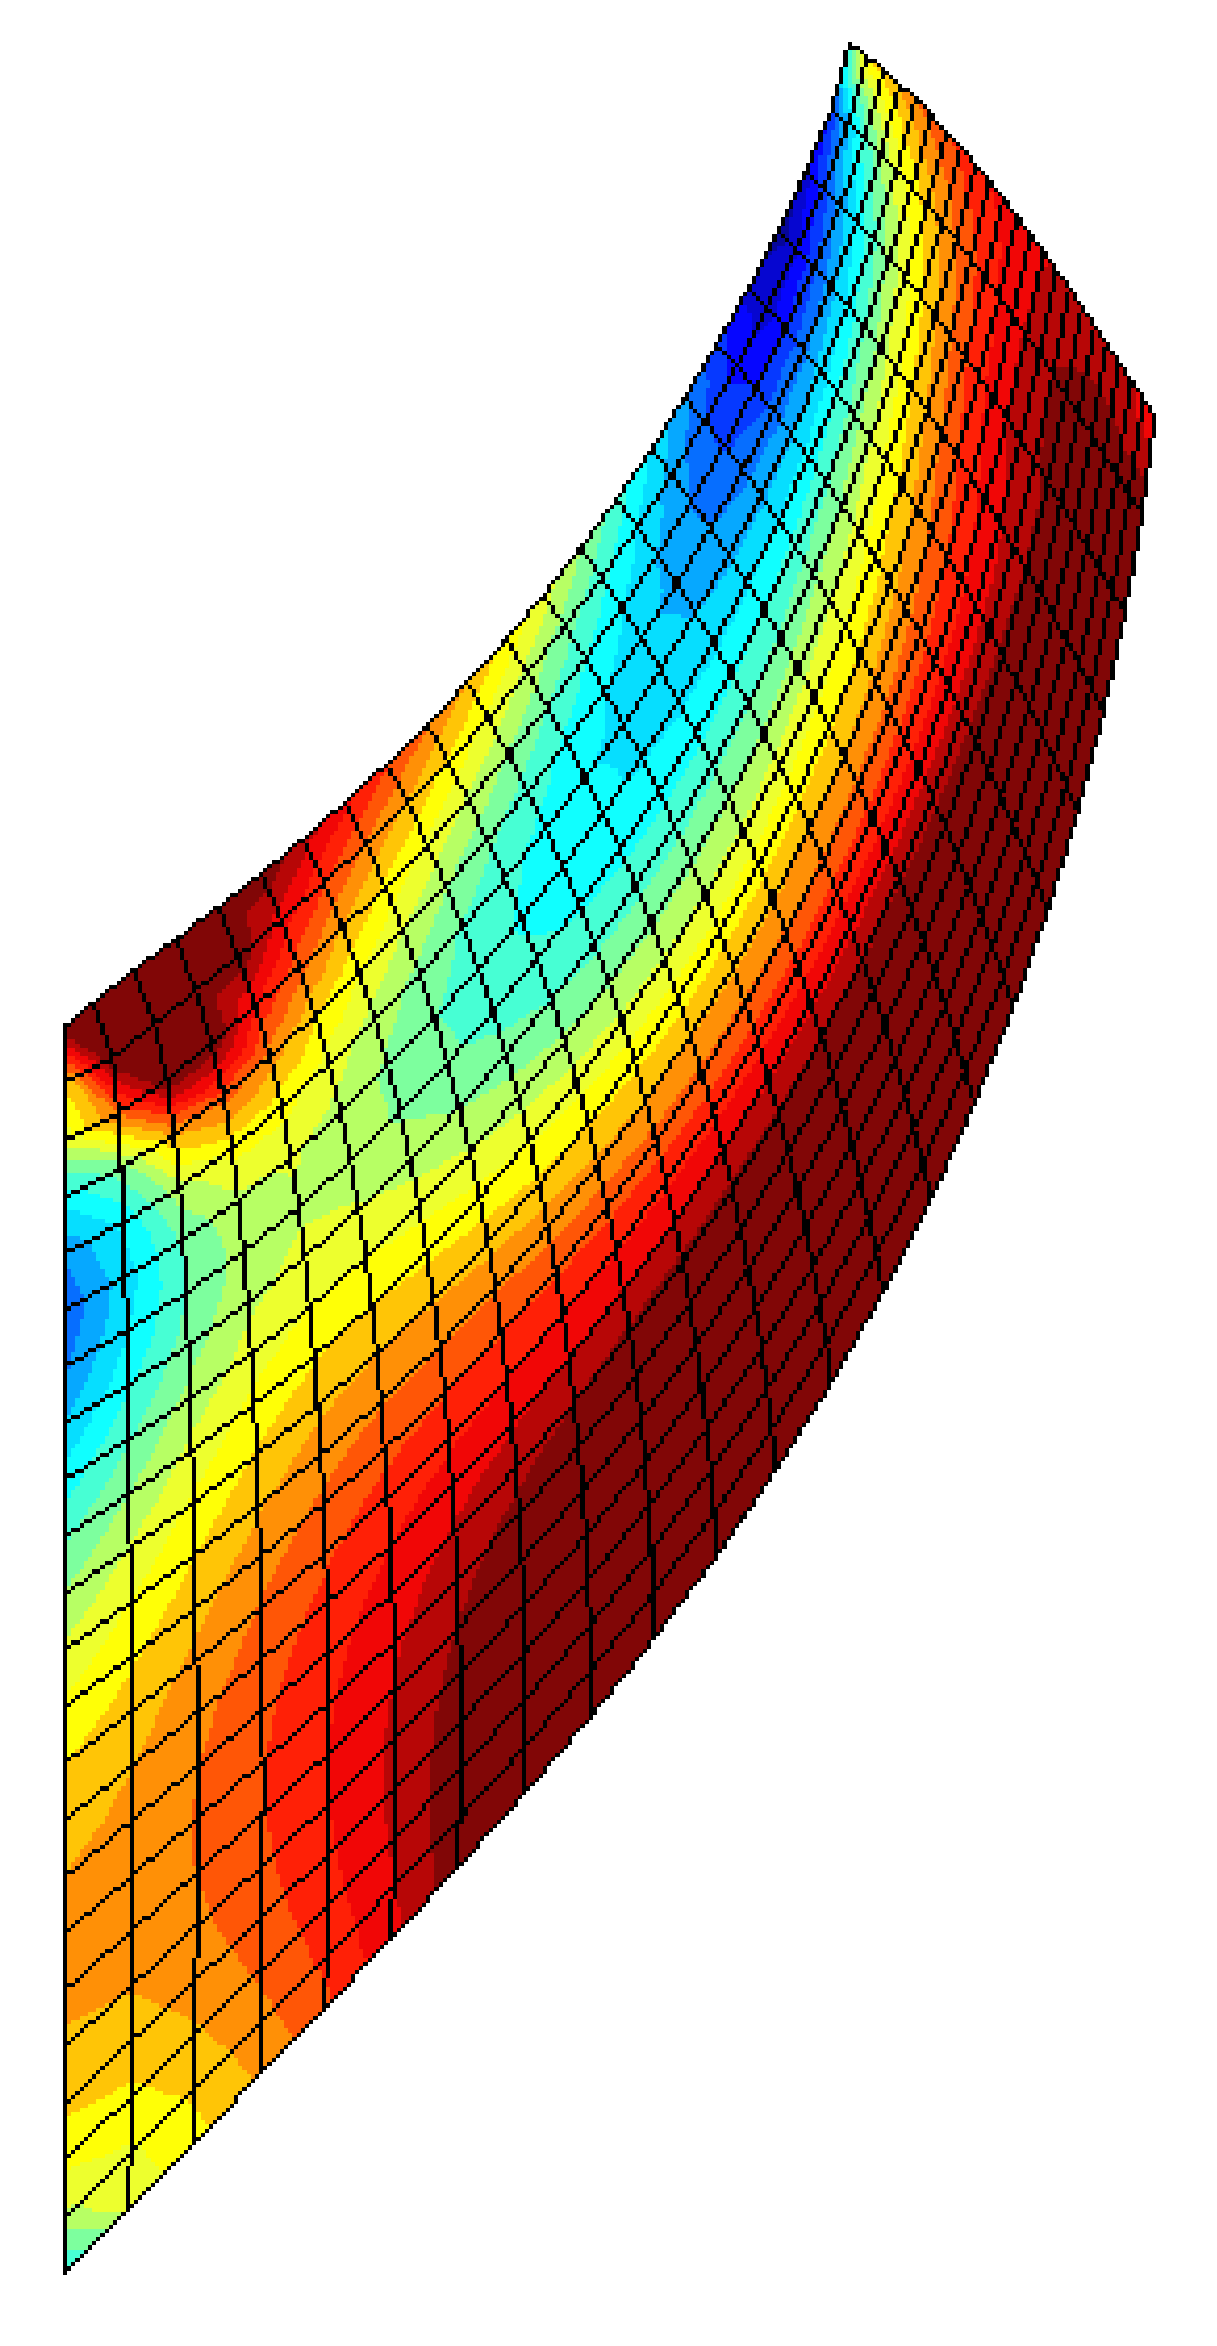
\includegraphics[width=.25\textwidth]{elemsolid}
\caption{Cook's membrane: deformed shape and VON MISES stress rendered using Gmsh}
\label{fig:EL:SOLID:COOKS-MEMBRANE}
\end{figure}
\clearpage



% Surface Load Elements
% MBDyn (C) is a multibody analysis code.
% http://www.mbdyn.org
%
% Copyright (C) 1996-2023
%
% Pierangelo Masarati  <pierangelo.masarati@polimi.it>
%
% Dipartimento di Ingegneria Aerospaziale - Politecnico di Milano
% via La Masa, 34 - 20156 Milano, Italy
% http://www.aero.polimi.it
%
% Changing this copyright notice is forbidden.
%
% This program is free software; you can redistribute it and/or modify
% it under the terms of the GNU General Public License as published by
% the Free Software Foundation (version 2 of the License).
%
%
% This program is distributed in the hope that it will be useful,
% but WITHOUT ANY WARRANTY; without even the implied warranty of
% MERCHANTABILITY or FITNESS FOR A PARTICULAR PURPOSE.  See the
% GNU General Public License for more details.
%
% You should have received a copy of the GNU General Public License
% along with this program; if not, write to the Free Software
% Foundation, Inc., 59 Temple Place, Suite 330, Boston, MA  02111-1307  USA

\section{Surface Loads}
\label{sec:EL:SURFLOAD}

\emph{Author: Reinhard Resch}
\subsection{Pressure Loads}
Pressure loads are intended mainly to apply prescribed pressure boundary conditions at the surface of solid elements.
However, they could be used also for shell and membrane elements. The value of the pressure can be imposed
by means of a set of drive callers, or by means of a set of abstract nodes. By convention, pressure loads are always applied
in the opposite direction of the surface normal vector. So, it is important, that the surfaces are oriented properly
when creating the mesh (e.g. use \emph{ReorientMesh} in \htmladdnormallink{\texttt{Gmsh}}{https://gmsh.info/}).
See also table~\ref{sec:EL:SURFLOAD:elemtypes} for a list of supported elements.
\begin{Verbatim}[commandchars=\\\{\}]
  \bnt{elem_type} ::= \{ \kw{pressureq4} | \kw{pressureq8} | \kw{pressureq8r} | \kw{pressureq9} | \kw{pressuret6} \}

  \bnt{normal_arglist} ::=
  \bnt{struct_node_data} , \bnt{pressure_load_data} ;

  \bnt{struct_node_data} :: =
  (\ty{StructDispNode}) \bnt{struct_node_1_label} ,
  (\ty{StructDispNode}) \bnt{struct_node_2_label} ,
  ... ,
  (\ty{StructDispNode}) \bnt{struct_node_N_label}

  \bnt{pressure_load_data} :: =
  \{ \kw{from drives} , \bnt{press_drive_data} |
  \kw{from nodes}  , \bnt{press_node_data} \}

  \bnt{pressure_drive_data} :: =
  (\hty{DriveCaller}) \bnt{press_drive_1} ,
  (\hty{DriveCaller}) \bnt{press_drive_2} ,
  ... ,
  (\hty{DriveCaller}) \bnt{press_drive_N}

  \bnt{pressure_node_data} :: =
  (\ty{AbstractNode}) \bnt{press_node_1} ,
  (\ty{AbstractNode}) \bnt{press_node_2} ,
  ... ,
  (\ty{AbstractNode}) \bnt{press_node_N}

\end{Verbatim}

\subsubsection{Example:}
\begin{verbatim}
       drive caller: 1, string, "1.5 * Time";
       drive caller: 2, string, "2.5 * Time";
       drive caller: 3, string, "3.5 * Time";
       drive caller: 4, string, "4.5 * Time";

       pressureq4: 100, 1, 2, 3, 4, from nodes, 10, 11, 12, 13;

       pressureq4: 101, 5, 6, 7, 8, from drives,
                    reference, 1,
                    reference, 2,
                    reference, 3,
                    reference, 4;
\end{verbatim}

\subsection{Surface Traction's}
Surface traction's are similar to pressure loads but they do not necessarily act perpendicular to the surface.
So, they can be used to impose a prescribed shear stress at the surface of a solid body.
Actually there are absolute and relative surface traction's. Absolute surface traction's are applied with respect
to the global reference frame and do not change their direction and magnitude if the surface is moved
or deformed during the simulation. In contradiction to that, relative surface traction's are also applied with respect
to the global reference frame, but their direction and magnitude is changed similar to pressure loads, if the surface is deformed or moved.
See also table~\ref{sec:EL:SURFLOAD:elemtypes} for a list of supported elements.
\begin{Verbatim}[commandchars=\\\{\}]
  \bnt{elem_type} ::= \{ \kw{tractionq4} | \kw{tractionq8} | \kw{tractionq8r} | \kw{tractionq9} | \kw{tractiont6} \}

  \bnt{normal_arglist} ::=
      [ \kw{absolute} , ] \bnt{struct_node_data} , \kw{from drives} , \bnt{traction_load_data}
      [ , \kw{orientation}, \bnt{traction_orient_data} ] ;

      \bnt{struct_node_data} :: =
      (\ty{StructDispNode}) \bnt{struct_node_1_label} ,
      (\ty{StructDispNode}) \bnt{struct_node_2_label} ,
      ... ,
      (\ty{StructDispNode}) \bnt{struct_node_N_label}

      \bnt{traction_load_data} :: =
      (\htybty{TplDriveCaller}{Vec3}) \bnt{traction_stress_1} ,
      (\htybty{TplDriveCaller}{Vec3}) \bnt{traction_stress_2} ,
      ... ,
      (\htybty{TplDriveCaller}{Vec3}) \bnt{traction_stress_N}

      \bnt{traction_orient_data} :: =
      (\hty{OrientationMatrix}) \bnt{orientation_matrix_1} ,
      (\hty{OrientationMatrix}) \bnt{orientation_matrix_2} ,
      ... ,
      (\hty{OrientationMatrix}) \bnt{orientation_matrix_M}
\end{Verbatim}

\subsubsection{Example:}
\begin{verbatim}
       reference: 10,
                position, reference, global, null,
                orientation, reference, global, 1, 0., 1., 0.,
                                                2, 1., 0., 0.,
                velocity, reference, global, null,
                angular velocity, reference, global, null;

       ...

       template drive caller: 1, 3, component,
                string, "1.5 * Time",
                string, "2.5 * Time",
                string, "3.5 * Time";

       ...

       template drive caller: 4, 3, component,
                string, "4.5 * Time",
                string, "5.5 * Time",
                string, "6.5 * Time";

       tractionq4: 100, 1, 2, 3, 4, from drives,
                    reference, 1,
                    reference, 2,
                    reference, 3,
                    reference, 4,
                    orientation,
                       reference, 10, eye,
                       reference, 20, eye,
                       reference, 30, eye,
                       reference, 40, eye;
\end{verbatim}

\begin{table}[h!tp]
  \begin{tabular}[t]{|c|c|c|c|c|c|c|}
    \hline
    element type pressure & element type traction & nodes & node order & integration points & order & references \tabularnewline
    \hline
    \kw{pressureq4} & \kw{tractionq4} & 4 & \ref{fig:EL:SURFLOAD:QUADRANGLE4} & 4 & 1 & \cite{BATHE2016} \tabularnewline
    \hline
    \kw{pressureq8} & \kw{tractionq8} & 8 & \ref{fig:EL:SURFLOAD:QUADRANGLE8} & 9 & 2 & \cite{BATHE2016} \tabularnewline
    \hline
    \kw{pressureq8r} & \kw{tractionq8r} & 8 & \ref{fig:EL:SURFLOAD:QUADRANGLE8R} & 9 & 2 & \cite{DHONDT2004} \tabularnewline
    \hline
    \kw{pressureq9} & \kw{tractionq9} & 9 & \ref{fig:EL:SURFLOAD:QUADRANGLE9} & 9 & 2 & \cite{CODEASTERR30301} \tabularnewline
    \hline
    \kw{pressuret6} & \kw{tractiont6} & 6 & \ref{fig:EL:SURFLOAD:TRIANGLE6H} & 7 & 2 & \cite{CODEASTERR30301} \tabularnewline
    \hline
  \end{tabular}
  \caption{Finite Element Types for surface loads}
  \label{sec:EL:SURFLOAD:elemtypes}
\end{table}

\begin{figure}[htb]
  \begin{subfigure}{0.5\textwidth}
    \centering
    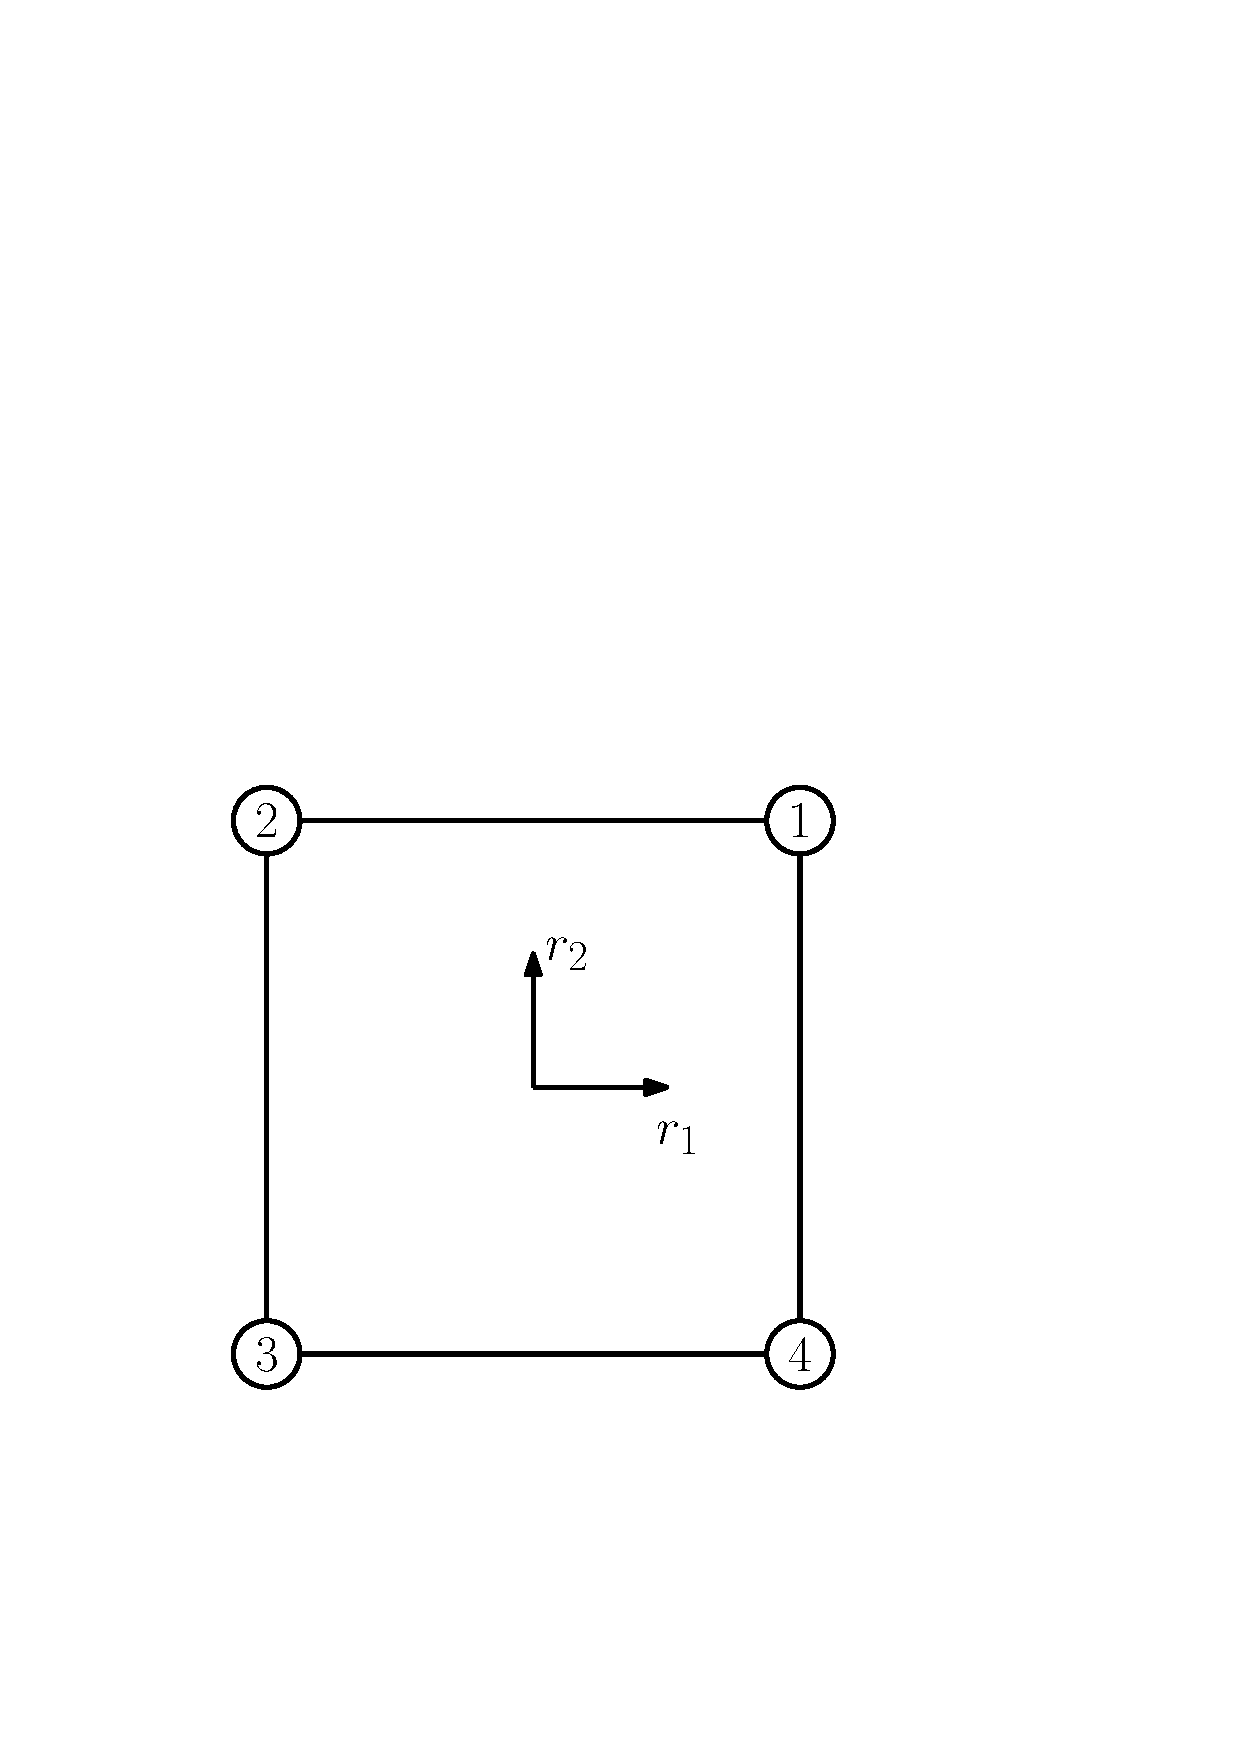
\includegraphics[width=0.5\textwidth]{quadrangle4}
    \caption{\kw{pressureq4}, \kw{tractionq4}}
    \label{fig:EL:SURFLOAD:QUADRANGLE4}
  \end{subfigure}
  \begin{subfigure}{0.5\textwidth}
    \centering
    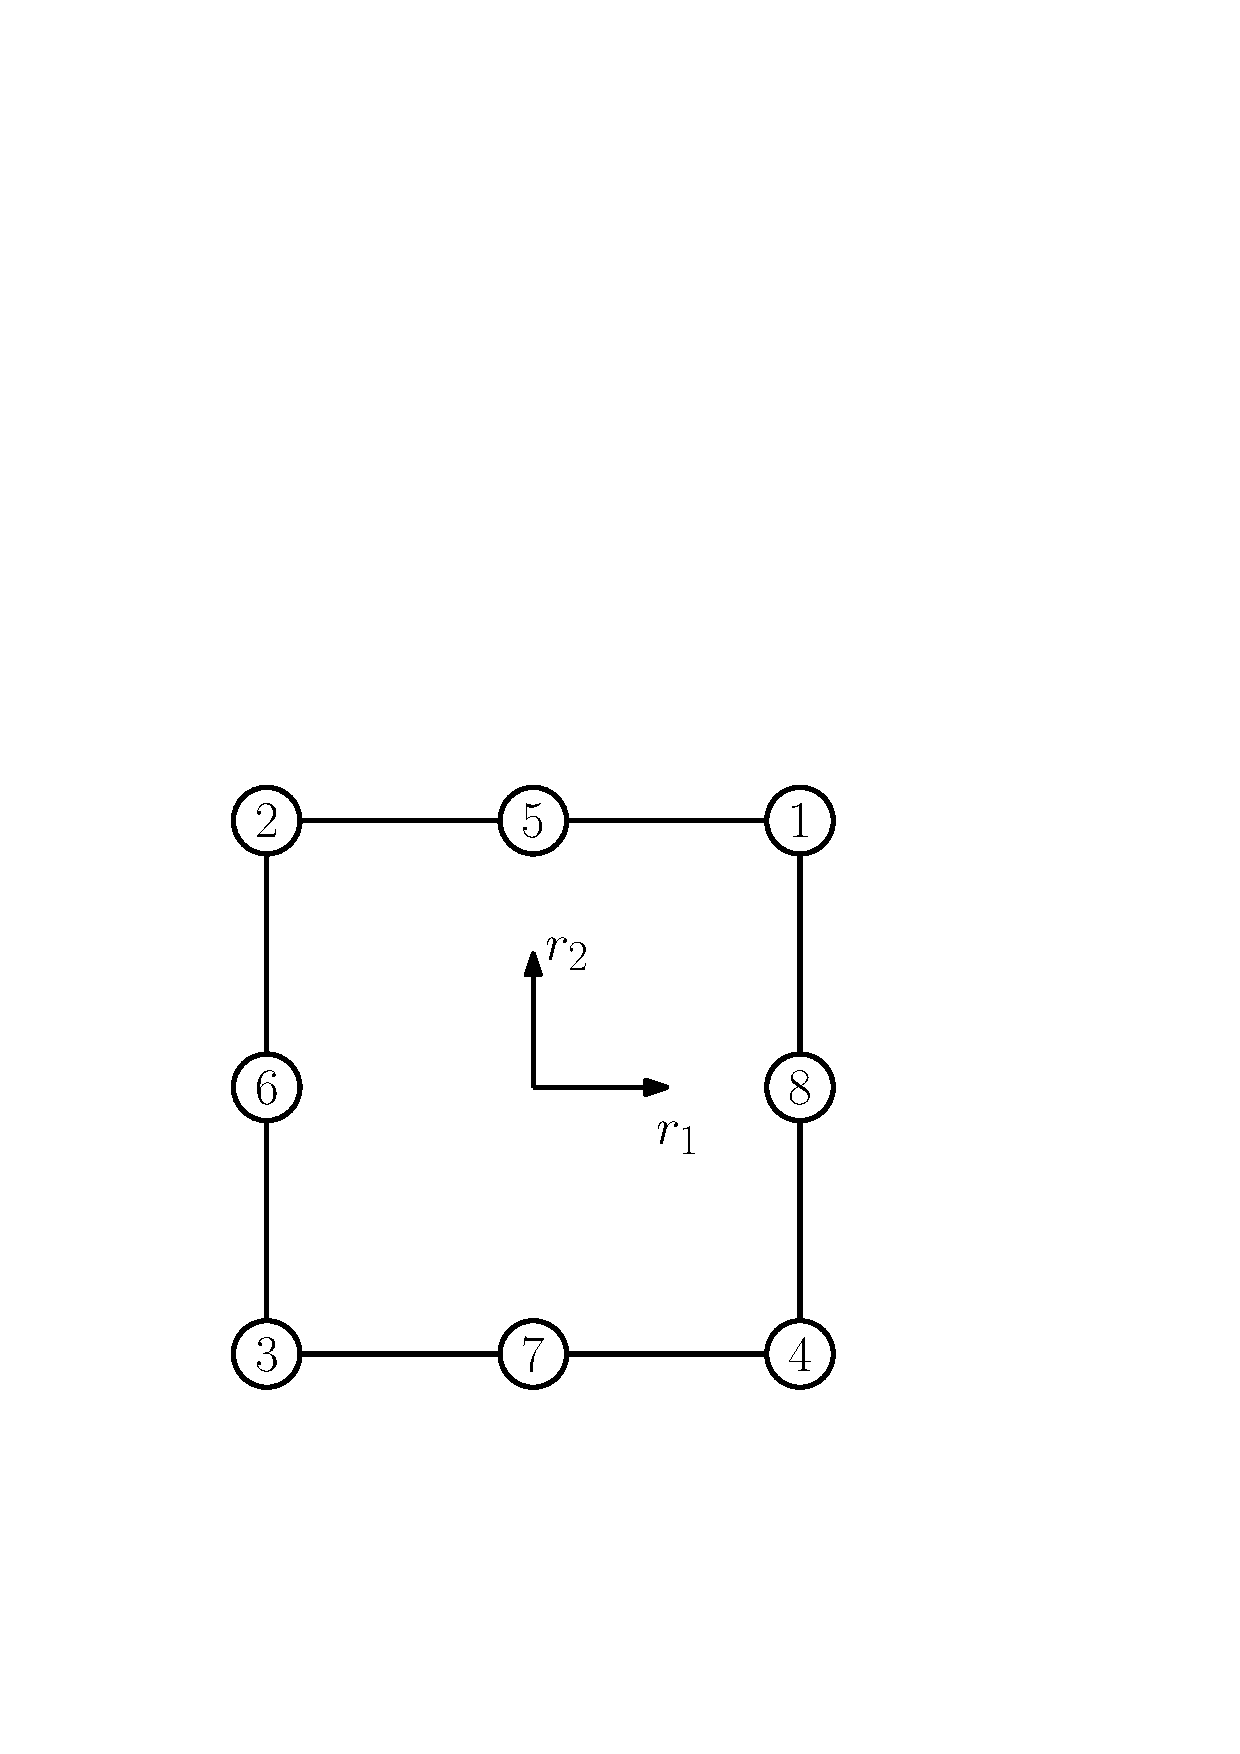
\includegraphics[width=0.5\textwidth]{quadrangle8}
    \caption{\kw{pressureq8}, \kw{tractionq8}}
    \label{fig:EL:SURFLOAD:QUADRANGLE8}
  \end{subfigure}
  \begin{subfigure}{0.5\textwidth}
    \centering
    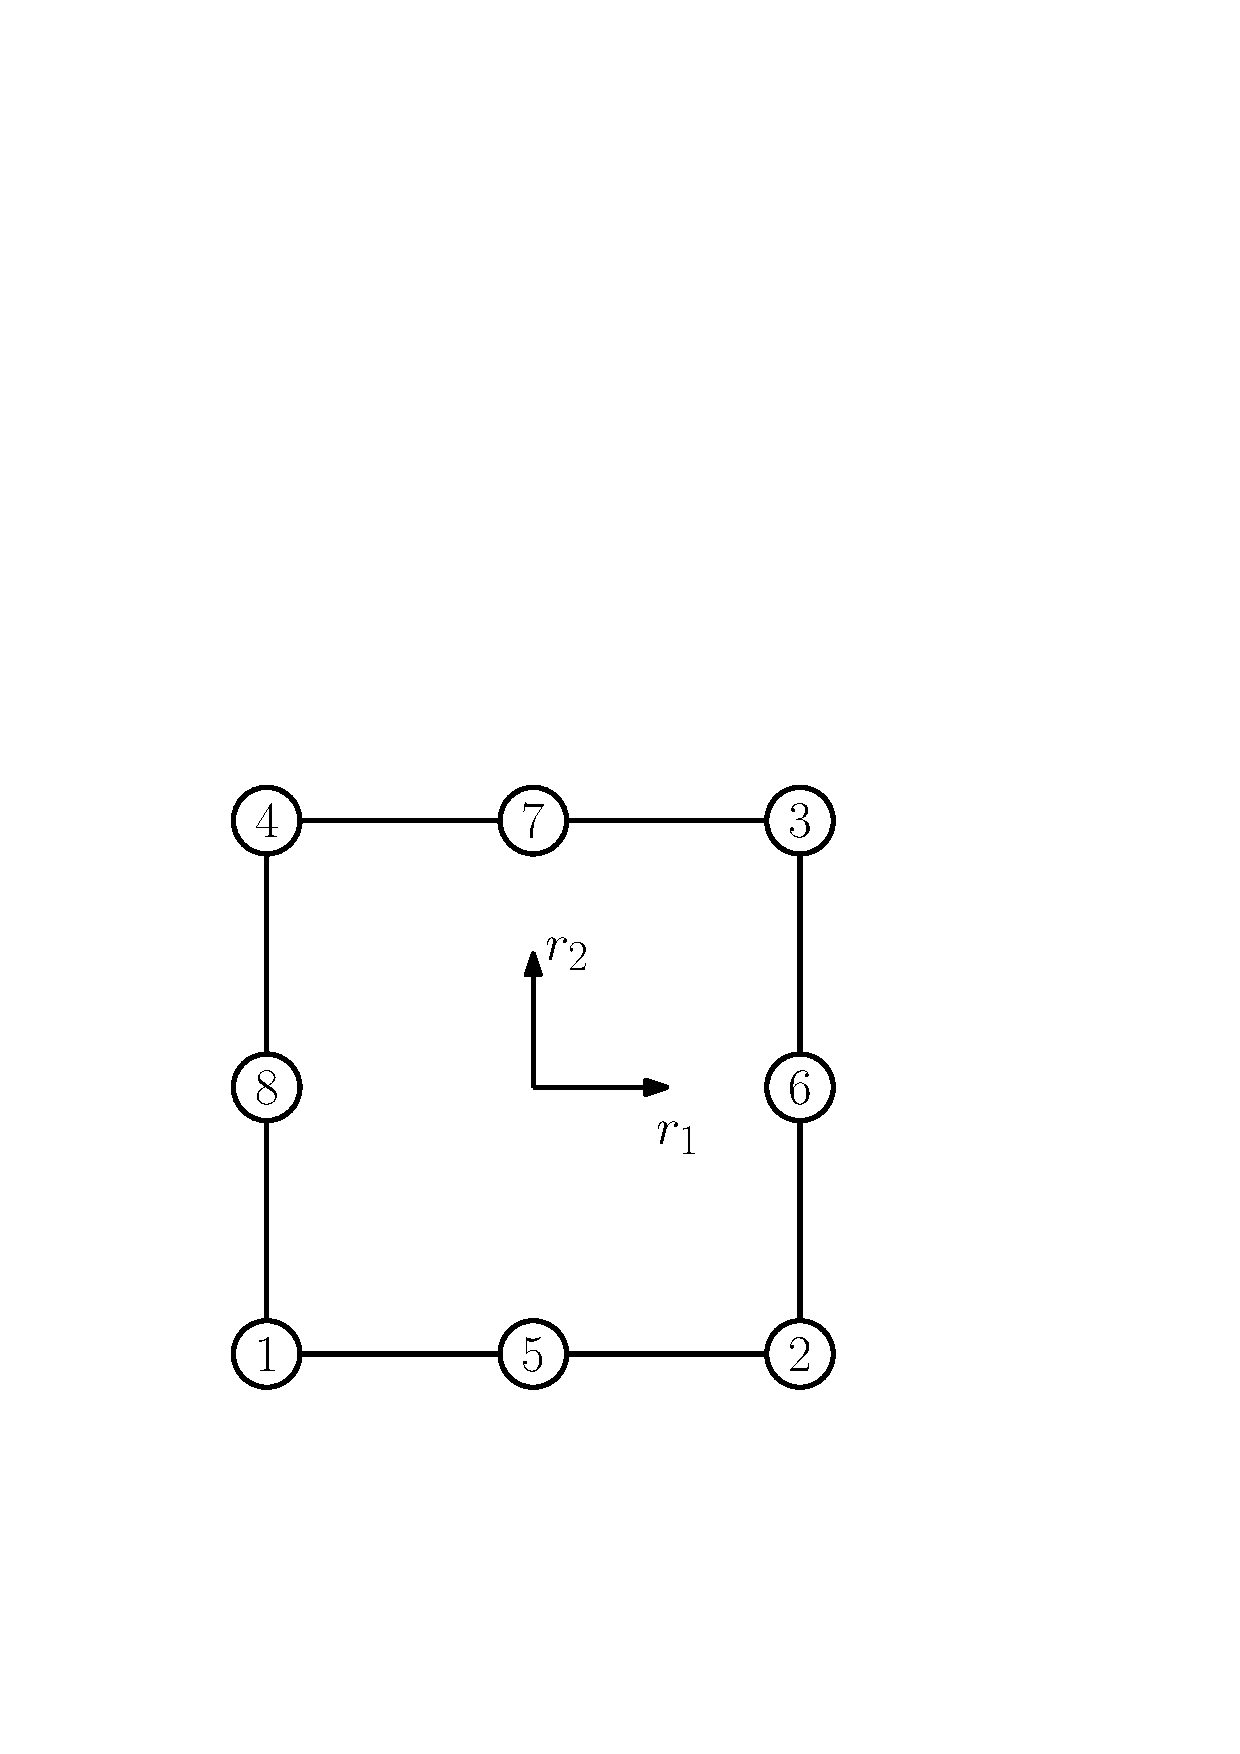
\includegraphics[width=0.5\textwidth]{quadrangle8r}
    \caption{\kw{pressureq8r}, \kw{tractionq8r}}
    \label{fig:EL:SURFLOAD:QUADRANGLE8R}
  \end{subfigure}
  \begin{subfigure}{0.5\textwidth}
    \centering
    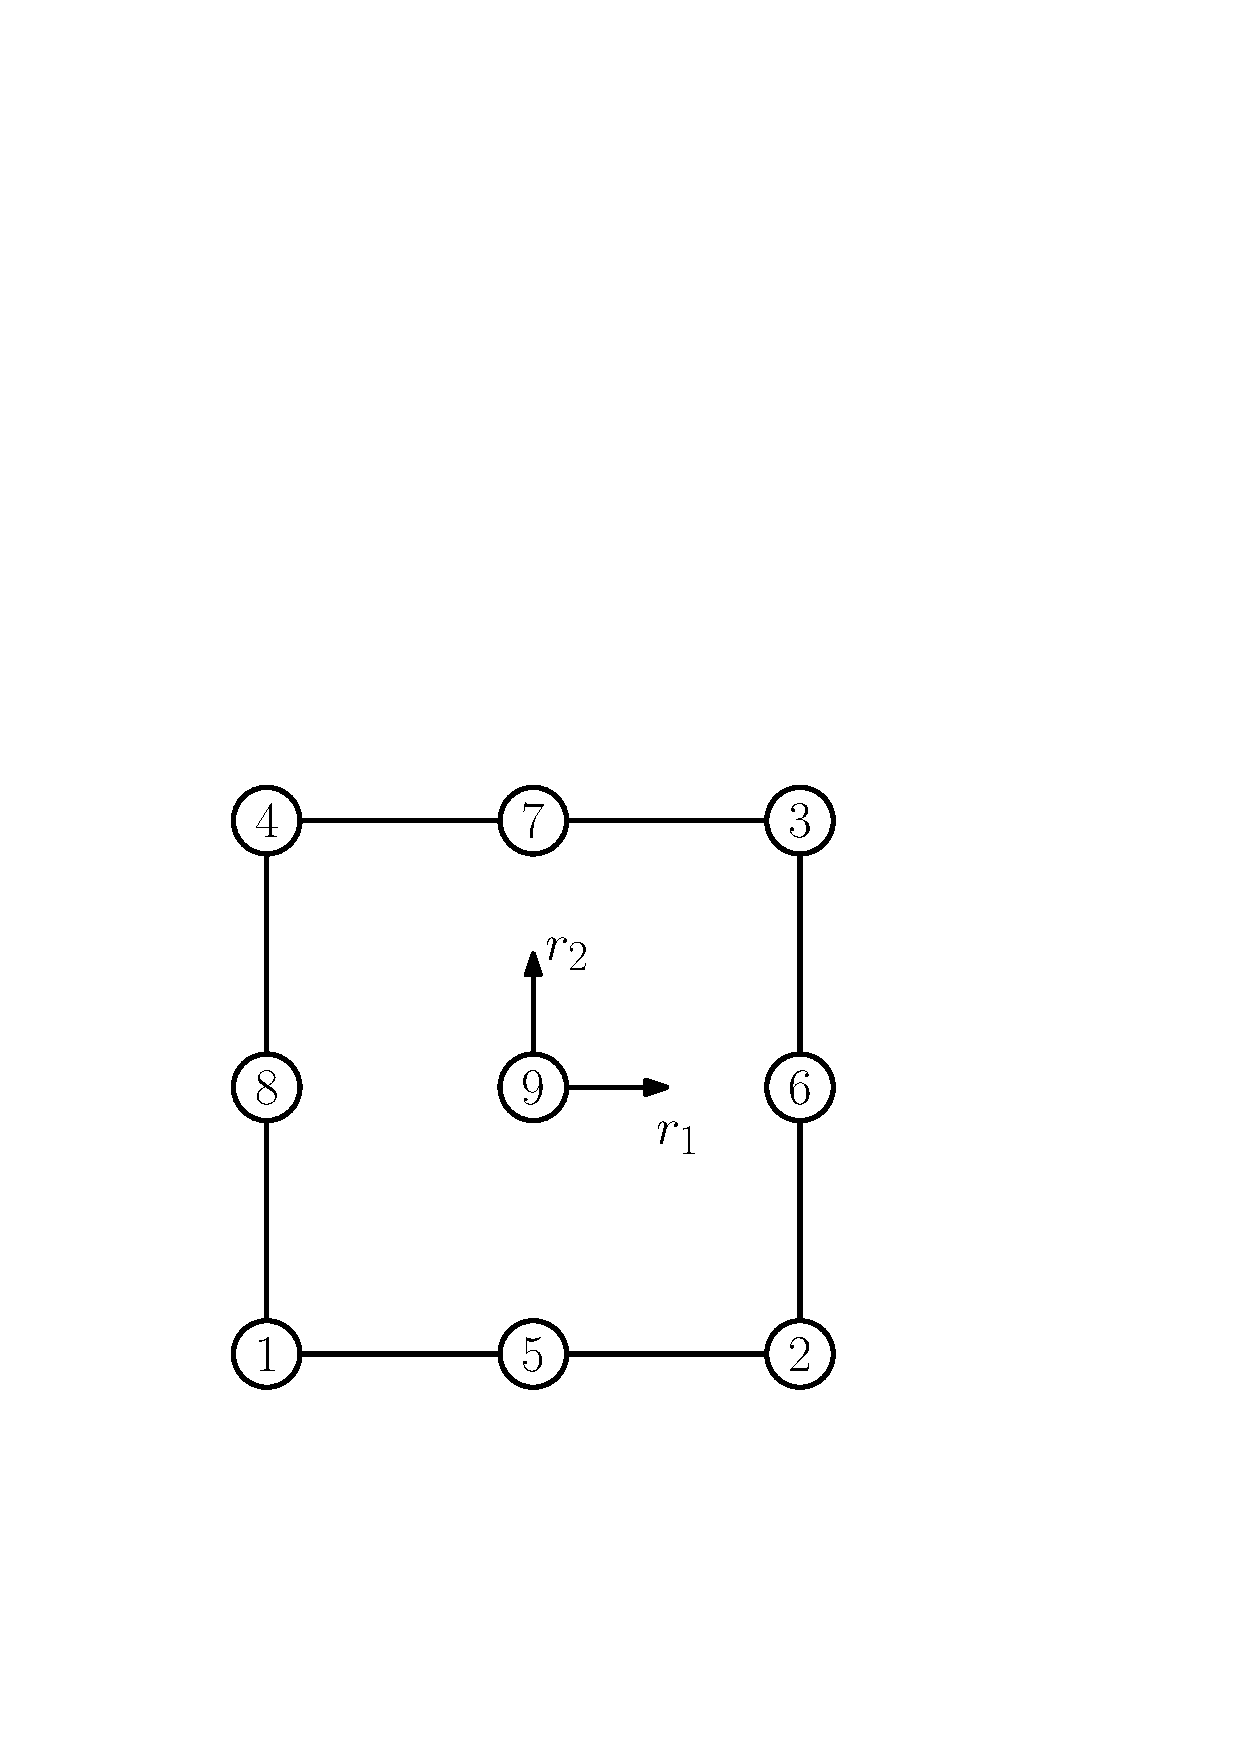
\includegraphics[width=0.5\textwidth]{quadrangle9}
    \caption{\kw{pressureq9}, \kw{tractionq9}}
    \label{fig:EL:SURFLOAD:QUADRANGLE9}
  \end{subfigure}
  \begin{subfigure}{0.5\textwidth}
    \centering
    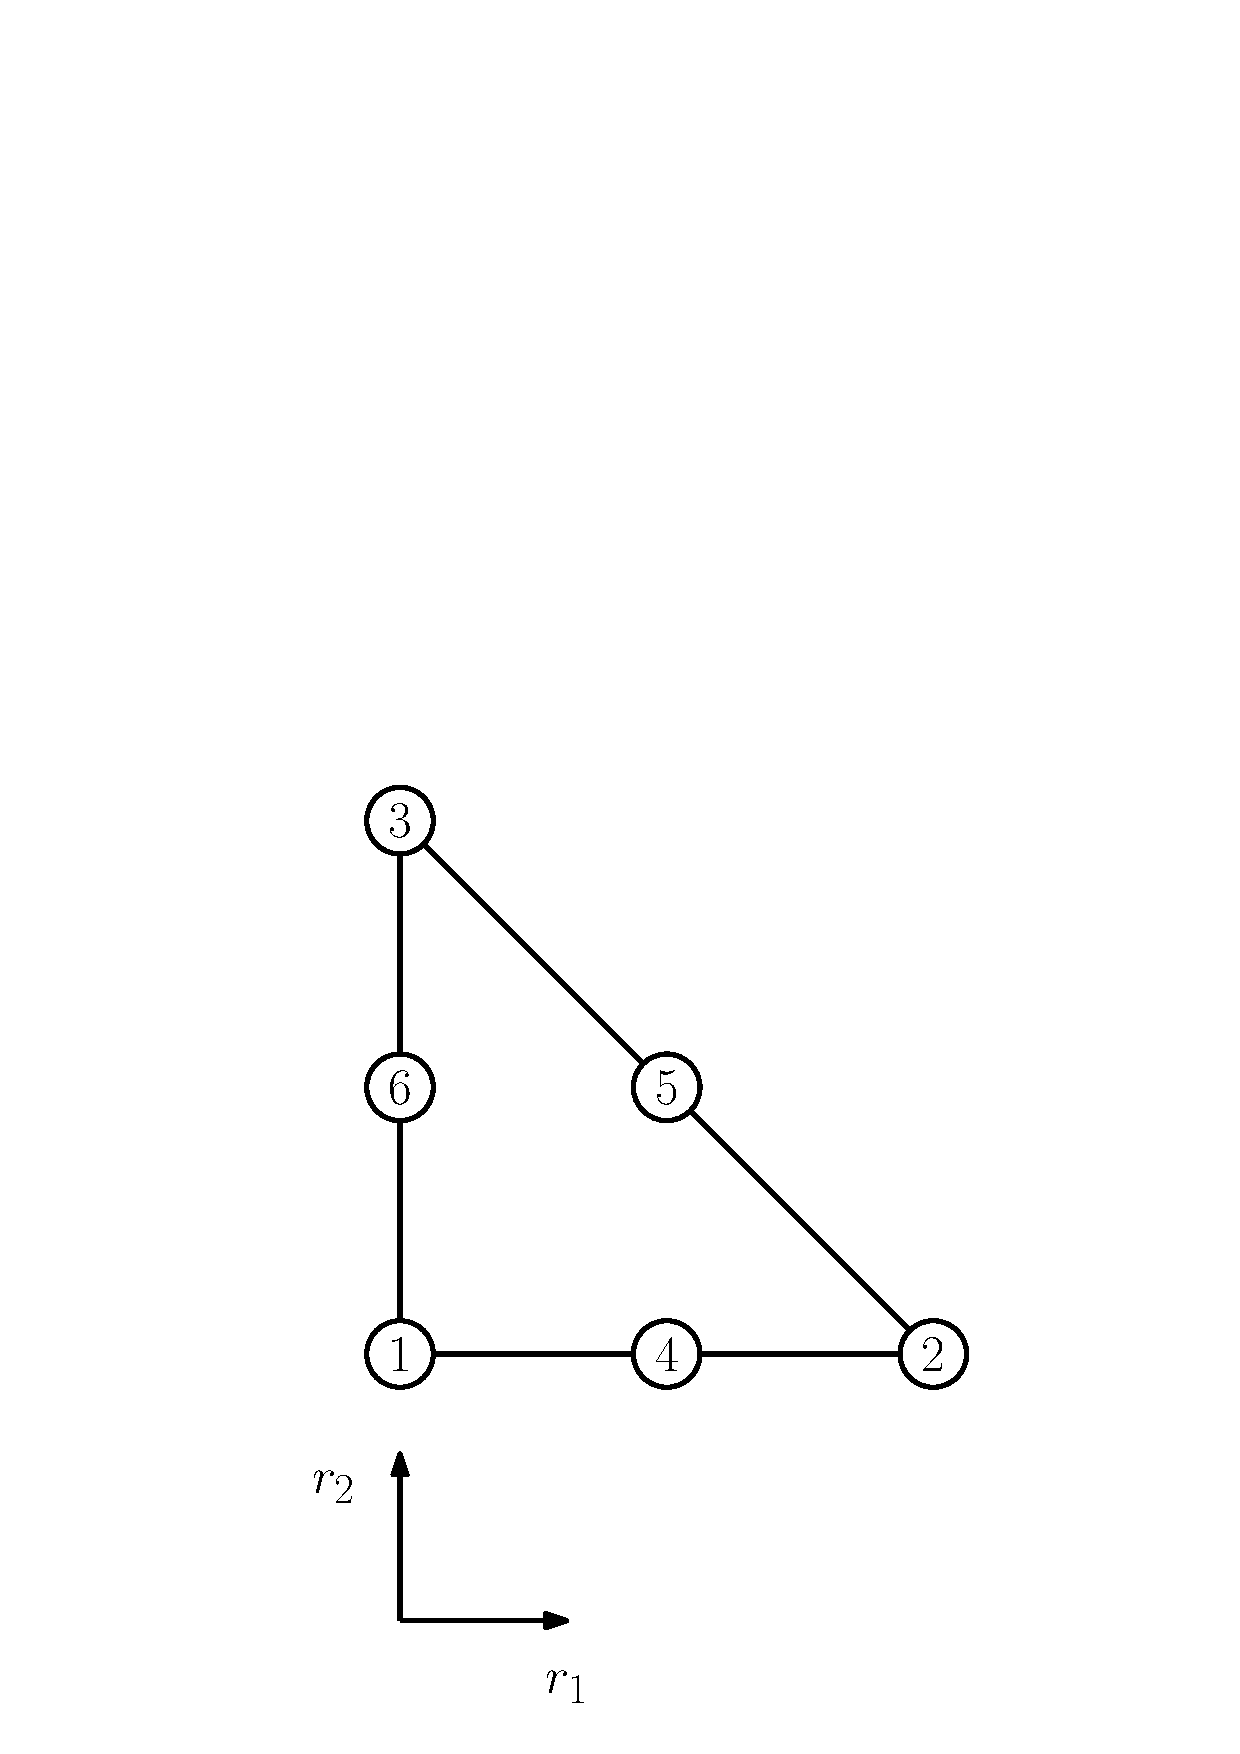
\includegraphics[width=0.5\textwidth]{triangle6h}
    \caption{\kw{pressuret6}, \kw{tractiont6}}
    \label{fig:EL:SURFLOAD:TRIANGLE6H}
  \end{subfigure}
  \caption{Node order: surface loads}
  \label{fig:EL:SURFLOAD:NODE_ORDER}
\end{figure}
\clearpage



% Thermal elements
% MBDyn (C) is a multibody analysis code.
% http://www.mbdyn.org
%
% Copyright (C) 1996-2023
%
% Pierangelo Masarati  <pierangelo.masarati@polimi.it>
%
% Dipartimento di Ingegneria Aerospaziale - Politecnico di Milano
% via La Masa, 34 - 20156 Milano, Italy
% http://www.aero.polimi.it
%
% Changing this copyright notice is forbidden.
%
% This program is free software; you can redistribute it and/or modify
% it under the terms of the GNU General Public License as published by
% the Free Software Foundation (version 2 of the License).
%
%
% This program is distributed in the hope that it will be useful,
% but WITHOUT ANY WARRANTY; without even the implied warranty of
% MERCHANTABILITY or FITNESS FOR A PARTICULAR PURPOSE.  See the
% GNU General Public License for more details.
%
% You should have received a copy of the GNU General Public License
% along with this program; if not, write to the Free Software
% Foundation, Inc., 59 Temple Place, Suite 330, Boston, MA  02111-1307  USA

\section{Thermal Elements}
\label{sec:EL:THERMO}

\subsection{Capacitance}
\label{sec:EL:THERMO:CAPACITANCE}

This element implements a simple linear thermal capacitance associated with a thermal node.
It computes the heat flow into the capacitance node as
\begin{align*}
	q &= -\nt{dCapacitance} \cdot \dot{T}
\end{align*}

The input format is:
%\begin{verbatim}
\begin{Verbatim}[commandchars=\\\{\}]
    \bnt{elem_type} ::= \kw{capacitance}

    \bnt{normal_arglist} ::= 
        \bnt{node_label} , 
        (\ty{real}) \bnt{dCapacitance}
\end{Verbatim}
%\end{verbatim}
where \nt{node\_label} is the thermal node the thermal capacitance is connected to, and \nt{dCapacitance} is the (positive) value of the thermal capacitance.

\paragraph{Example.} \
\begin{verbatim}
    thermal: 99, capacitance,
        11,    # node label
        0.11;  # capacitance
\end{verbatim}



\subsection{Resistance}
\label{sec:EL:THERMO:RESISTANCE}

This element implements a simple linear thermal resistance between two thermal nodes.
It computes the heat flow between the two nodes as
\begin{align*}
	q_{21} &= \frac{T_2 - T_1}{\nt{dResistance}}
\end{align*}

The input format is:
%\begin{verbatim}
\begin{Verbatim}[commandchars=\\\{\}]
    \bnt{elem_type} ::= \kw{resistance}

    \bnt{normal_arglist} ::= 
        \bnt{node_1_label} , 
        \bnt{node_2_label} , 
        (\ty{real}) \bnt{dResistance}
\end{Verbatim}
%\end{verbatim}
where \nt{node\_1\_label} and \nt{node\_2\_label} are the thermal nodes the thermal resistance is connected to, and \nt{dResistance} is the (positive) value of the thermal resistance.

\paragraph{Example.} \
\begin{verbatim}
    thermal: 98, resistance,
        11,    # node 1 label
        12,    # node 2 label
        0.99;  # resistance
\end{verbatim}



\subsection{Source}
\label{sec:EL:THERMO:SOURCE}

This element implements a simple thermal source associated with a thermal node.
It computes the heat flow into the node as
\begin{align*}
	q &= \nt{Source}
\end{align*}

The input format is:
%\begin{verbatim}
\begin{Verbatim}[commandchars=\\\{\}]
    \bnt{elem_type} ::= \kw{capacitance}

    \bnt{normal_arglist} ::= 
        \bnt{node_label} , 
        (\hty{DriveCaller}) \bnt{Source}
\end{Verbatim}
%\end{verbatim}
where \nt{node\_label} is the thermal node the thermal source is connected to, and \nt{Source} is a \ty{DriveCaller}.

\paragraph{Example.} \
\begin{verbatim}
    thermal: 97, source,
        12,    # node label
        # source; grows as 1-cos from 0 s to 1 s, raising from 0. to 0.9 
        cosine, 0., pi, 0.45, half, 0.;
\end{verbatim}








% User-Defined Elements
\section{User-Defined Elements}\label{sec:EL:BASE:USER_DEFINED}

\subsection{Loadable Element}\label{sec:EL:BASE:USER_DEFINED:LOADABLE}
Note: the \kw{loadable} element is deprecated in favor
of the \kw{user defined} element.

The \kw{loadable} element is a wrapper for a user-defined element that is
compiled in a separated module and linked run-time.
The module should provide a comprehensive set of functions according to 
a specified API; default functions are available if no special features
are required.
Implementation of modules can be very easy, but a deep knowledge of the
internals of the code is required when special tasks need to be performed. 
There are virtually no limits on what a loadable element can do.

The syntax is simply:
%\begin{verbatim}
\begin{Verbatim}[commandchars=\\\{\}]
    \bnt{elem_type} ::= \kw{loadable}

    \bnt{normal_arglist} ::= " \bnt{module_name} "
        [ , \kw{name} , " \bnt{calls} " ] 
        [ , \bnt{module_data} ]
\end{Verbatim}
%\end{verbatim}
where \nt{module\_name} is the name of the module file; as soon as the file
is checked and the binding of the structure with function bindings 
succeeded, a function called \texttt{read()} is invoked, passing it the input
stream.
This function is in charge of reading \nt{module\_data} following the
general syntax of the input file.

An alternative form is
%\begin{verbatim}
\begin{Verbatim}[commandchars=\\\{\}]
    \bnt{normal_arglist} ::= \kw{reference} , " \bnt{name} "
        [ , \bnt{module_data} ]
\end{Verbatim}
%\end{verbatim}
where \nt{name} is the name by which the loadable element recorded itself
when registered via the \kw{module load} directive, as described
in Section~\ref{sec:GENERAL:MODULE-LOAD}.
As a consequence, the following forms are equivalent:
\begin{verbatim}
    # direct runtime loading
    loadable: 1, "/some/module.so";
    # "/some/module.so" registers itself as "some_module"
    module load: "/some/module.so";
    loadable: 2, reference, "some_module";
    # works also as joint (might obsolete loadable elements)
    joint: 3, some_module;
\end{verbatim}

It is advisable that the function \texttt{read()} prints some help message
when the first field of \nt{module\_data} is the keyword \kw{help}.
All the helpers and the high-level structures are available, such as
drivers, constitutive laws, reference frames.
Refer to each module for a description (if available) of the features and of
the input/output format.
\nt{module\_name} should be a full path to the module function.
If the name starts with a slash ``/'', the full path name is used.
Otherwise the module is searched in the colon-separated list of directories 
contained in the environment variable \texttt{LD\_LIBRARY}, then among the
libraries listed in \texttt{/etc/ld.so.cache}, and finally in
\texttt{/usr/lib} and in \texttt{/lib} (see \texttt{dlopen(3)}).
At last, it is searched in the current directory, and the extension
\texttt{.so} is added if missing.
The string \nt{calls} represents the name of the structure that contains
the bindings to the functions.
The default is \texttt{calls}.

\noindent
Refer to \texttt{\$(BASE)/mbdyn/base/loadable.h} for a description of the
functions that are allowed.
An example module is given in directory
\begin{verbatim}
    $(BASE)/modules/module-template/
\end{verbatim}
which can be used as a starting point to build a custom module.
% An analogous C/FORTRAN style interface is being planned, at the cost of
% possibly losing some of the fancy C++ features made available by the code.
The \kw{loadable} element interface allows to link modules in different
languages, e.g.\ C or FORTRAN77; simply use \texttt{module-template}
as a guideline to providing callbacks to the \kw{loadable} element
interface and to collect required info from the main program
(e.g.\ node positions, equation indices and everything else that is
required for appropriate connection), then call the functions that
actually do the work in other languages from inside the callbacks.

\subsection{User-Defined Element}
The \kw{user defined} element is a much more streamlined form
of custom element definition than the \kw{loadable} element.
From the point of view of the syntax the differences are minimal;
however, from an implementation point of view, the \kw{user defined}
element is preferable.

The definition of a \kw{user defined} element requires two steps.
In the first step, a run-time loadable module is loaded using the 
\hyperref{\kw{module load} directive}{\kw{module load} directive (see Section~}{)}{sec:GENERAL:MODULE-LOAD}.
This registers a handler to the \kw{user defined} element type
along with a \nt{name} used to reference it.
In the second step, an instance of that \kw{user defined} element type
is created, referencing it by \nt{name}.

The syntax of the \kw{user defined} element is
%\begin{verbatim}
\begin{Verbatim}[commandchars=\\\{\}]
    \bnt{elem_type} ::= \kw{user defined}

    \bnt{normal_arglist} ::= \bnt{name} [ , \bnt{module_data} ]
\end{Verbatim}
%\end{verbatim}
As for the \kw{loadable} element, it is recommended that 
some useful output is given if the first \nt{module\_data}
is the keyword \kw{help}.

An example module is given in directory
\begin{verbatim}
    $(BASE)/modules/module-template2/
\end{verbatim}
which can be used as a starting point to build a custom module.

\paragraph{Example.} \
\begin{verbatim}
    module load: "libmodule-template2";

    user defined: 1000, template2, help;
\end{verbatim}



\subsection{General Discussion on Run-Time Loadable Modules}
In general, to call external functions from C++ one needs
to declare them as
\begin{verbatim}
    #include <sys/types.h>
    extern "C" {
        int a_C_function(int arg, double darg);
        int a_F77_subroutine(int32_t *iarg, double *darg);
    }
\end{verbatim}
The same applies to FORTRAN 77 functions; only, the naming convention
usually is compiler dependent; some compilers turn all the names to 
uppercase or lowercase (remember that FORTRAN 77 is case insensitive);
other compilers add underscores at the beginning or at the end of the
names.
Check what is the behavior of your compiler, by compiling a simple 
program with your favorite FORTRAN 77 compiler, then looking at it
with the utility \texttt{nm(1)}, which will show how the symbols are represented 
internally.

\noindent
For instance, the code
\begin{verbatim}
C This is a compiler test
      SUBROUTINE F77SUB(I, D)
      INTEGER*4 I
      REAL*8 D(*)

      D(I) = 0.0

      END
\end{verbatim}
when compiled with \texttt{g77(1)} on a GNU/Linux system, yields:
\begin{verbatim}
[masarati@mbdyn manual]$ g77 -c f77sub.f
[masarati@mbdyn manual]$ nm f77sub.o
00000000 T f77sub_
\end{verbatim}
That is, \texttt{g77(1)} lowercases all symbols, and adds a trailing 
underscore.
Macros to automatically detect and take care of this behavior 
are planned.


\noindent
To compile loadable modules, one needs to configure
the package as follows:
%\begin{verbatim}
\begin{Verbatim}[commandchars=\\\{\}]
    ./configure --with-module=\bnt{module_name}
\end{Verbatim}
%\end{verbatim}
where \nt{module\_name} is the name of the directory the module
is placed in with the \texttt{module-} part stripped; e.g.\ to compile
the tire module that resides in \texttt{\$(BASE)/modules/module-wheel2} 
one must type
\begin{verbatim}
    ./configure --with-module=wheel2
\end{verbatim}
Multiple modules can be compiled by typing the list of the names
separated by blanks.

\bigskip

\noindent
\fbox{\begin{minipage}{.96\textwidth}
The modules need to resolve some of the symbols that are in the
main executable; until a full working libtool support is implemented,
this must be done by hand.
The \texttt{g++(1)} compiler requires the switch `\texttt{-rdynamic}'
to be added to the loader's flags.
\end{minipage}}

\bigskip

For example,
%\begin{verbatim}
\begin{Verbatim}[commandchars=\\\{\}]
    ./configure --with-module=\bnt{module_name} LDFLAGS="-rdynamic" 
\end{Verbatim}
%\end{verbatim}




\section{Miscellaneous}
This section lists some extra cards that do not correspond to any
specific simulation entity, but rather alter the behavior 
of existing entries or cause special operations to be undertaken
during model input.



\subsection{Bind}\label{sec:EL:MISC:BIND}
The statement \kw{bind} does not really define an element.
It is rather used to instruct a
\htmlref{\kw{parameter node}}{sec:NODE:PARAMETER}
about which parameter of an element it is bound to.
The \kw{parameter node} must exist, and the element the node 
is being bound to, of type \nt{elem\_type} and label \nt{element\_label},
must have been already defined.
The complete syntax is:
%\begin{verbatim}
\begin{Verbatim}[commandchars=\\\{\}]
    \bnt{elem_type} ::= \kw{bind}

    \bnt{arglist} ::=
        \bnt{element_label} ,
        \bnt{element_type} ,
        \bnt{parameter_node_label} , 
        \bnt{bind_args}
\end{Verbatim}
%\end{verbatim}
where \nt{bind\_args} depend on the type of parameter node.

\subsubsection{Element}
When binding an element to an 
\htmlref{\kw{element}}{sec:NODE:PARAMETER:ELEMENT} parameter node,
each element makes a number of specific parameters available.
A detailed list is given for each element in the private data section.
In that case:
%\begin{verbatim}
\begin{Verbatim}[commandchars=\\\{\}]
    \bnt{bind_args} ::=
        \{ [ \kw{index} , ] \bnt{parameter_index}
            | \kw{string} , " \bnt{parameter_name} " \}
\end{Verbatim}
%\end{verbatim}
The value of \nt{parameter\_index} must be legal, i.e.\ between 1 and the
maximum number of parameters made available by the element.
The alternative form, using the keyword \kw{string} followed by
the \nt{parameter\_name}, allows more friendly definition of the binding.
The name of the parameter depends on the element whose property
is being bound.
A complete listing of the parameters that a parameter node 
can be bound to can be found in the `Private data' subsection
of each element's specification.

\paragraph{Example.} \
The parameter node \texttt{ANGLE} is bound to the rotation of a 
\hyperref{\kw{revolute hinge}}{\kw{revolute hinge} (see Section~}{)}{sec:EL:STRUCT:JOINT:REVOLUTE_HINGE}.
\begin{verbatim}
    # ... problem block

    begin: control data;
        structural nodes: 2;
        parameter nodes: 1;
        forces: 2;
        # ... other control data
    end: control data;

    set: integer NODE1 = 1000;
    set: integer NODE2 = 2000;
    set: integer ANGLE = 5000;
    set: integer REVOLUTE = 6000;

    begin: nodes;
        structural: NODE1, dynamic, null, eye, null, null;
        structural: NODE2, dynamic, null, eye, null, null;
        parameter: ANGLE, element;

        # ... other nodes
    end: nodes;

    begin: elements;
        joint: REVOLUTE, revolute hinge,
            NODE1,
                position, reference, node, null,
                orientation, reference, node, eye,
            NODE2,
                position, reference, node, null,
                orientation, reference, node, eye;
        bind: REVOLUTE, joint, ANGLE, string, "rx";
        couple: 1, NODE1, 0.,0.,1.,
            dof, ANGLE, parameter, 1, linear, 0.,1.;
        couple: 2, NODE2, 0.,0.,1.,
            element, REVOLUTE, joint, string, "rx", linear, 0.,1.;

        # ... other elements
    end: elements;
\end{verbatim}
Note that the same element data, i.e.\ the revolute hinge
relative rotation angle, is used to drive a couple in two different
ways; the latter, by means of the 
\hyperref{\kw{element} drive}{\kw{element} drive (see Section~}{)}{sec:DriveCaller:ELEMENT}
is more direct, but the former, by means of the 
\hyperref{\kw{dof} drive}{\kw{dof} drive (see Section~}{)}{sec:DriveCaller:DOF}
through the \kw{bind} mechanism has the additional effect of updating
the \kw{parameter} node, which can be used to connect
\htmlref{\kw{genel}}{sec:EL:GENEL} elements for special purposes.

\subsubsection{Beam strain gage}
When binding an element to a
\htmlref{\kw{beam strain gage}}{sec:NODE:PARAMETER:BEAM_STRAIN_GAGE}
parameter node, the \nt{element\_type} field must be \kw{beam}.
In that case:
%\begin{verbatim}
\begin{Verbatim}[commandchars=\\\{\}]
    \bnt{bind_args} ::= \bnt{beam_evaluation_point}
\end{Verbatim}
%\end{verbatim}
where \nt{beam\_evaluation\_point} is the evaluation point of the beam element
where the internal strain and curvatures must be evaluated.
It must be 1 for 2-node beams, while it can be either 1 or 2
for 3-node beams.

\paragraph{Example.} \
\begin{verbatim}
    # ... problem block

    begin: control data;
        parameter nodes: 1;
        beams: 1;
        # ... other control data
    end: control data;

    set: integer BEAM = 100;
    set: integer STRAIN = 200;

    begin: nodes;
        parameter: STRAIN, beam strain gage, 0.0, 0.1;
        # ... other nodes
    end: nodes;

    begin: elements;
        beam3: BEAM, ...; # beam data
        bind: BEAM, beam, STRAIN, 1;
        # ... other elements
    end: elements;
\end{verbatim}



\subsection{Driven Element}\label{sec:EL:BASE:DRIVEN}
The \kw{driven} type is not an element by itself. It is a wrapper that
masks another element and switches it on and off depending on the (boolean)
value of a drive. It can be used to emulate a variable topology model,
where some elements simply don't contribute to the residual
or to the Jacobian matrices when their drive has a certain value.
Since the drivers can be arbitrary functions of the time, 
or other parameters including the value of any degree of freedom, 
the driven elements can be ``driven'' in a very flexible way.
Every element can be driven, except those that can be instantiated once only.
The syntax for a driven element is:
%\begin{verbatim}
\begin{Verbatim}[commandchars=\\\{\}]
    \bnt{elem_type} ::= \kw{driven}

    \bnt{normal_arglist} ::= (\hty{DriveCaller}) \bnt{element_driver} ,
        [ \kw{initial state} , \{ \kw{from drive} | \kw{active} | \kw{inactive} | (\ty{bool}) \bnt{state} \} ]
        [ \kw{hint} , " \bnt{hint} " [ , ... ] ] ,
        \bnt{driven_element}

    \bnt{driven_element} ::=
        \{ \kw{existing} : \bnt{driven_elem_type} , \bnt{driven_elem_label}
            | \bnt{element_card} \}
\end{Verbatim}
%\end{verbatim}
When the keyword \kw{existing} is used, an existing element 
of type \nt{driven\_elem\_type} and label \nt{driven\_elem\_label} is looked for, 
and it is wrapped by the driven element.
In this case, no new element is instantiated.
The label of the element must match that of the driving element given 
at the beginning.
For consistency with the syntax, and for more flexibility, 
even when wrapping an existing element the output flags can be set
at the end of the card.
This flag overrides the one set when the driven element was instantiated.

The \kw{initial state} keyword overrides the evaluation of the \nt{element\_driver}
during the initialization.  The value \kw{from drive} is the default behavior;
the other keywords and the boolean value \nt{state} are self-explanatory.

Otherwise, a regular element is read after the driving element's declaration;
it is then instantiated and wrapped by the \kw{driven} element wrapper.
Note that after the keyword \kw{existing} or after the driven element type,
a colon is used as a separator.
This is probably the only exception to the rule that the colon
can only follow a \nt{description} at the beginning of a card.
The label \nt{driven\_elem\_label} of the driven element must match that
of the driving element used at the beginning of the \kw{driven} card.

\paragraph{Example.} \
A pin constraint between two rigid bodies is released:
\begin{verbatim}
    set: integer BODY_1 = 1;
    set: integer BODY_2 = 2;
    # ...
    structural: BODY_1, dynamic,
        null, eye, null, null;
    structural: BODY_2, dynamic,
        null, eye, null, null;
    # ....
    body: BODY_1, BODY_1,
        1000., null, diag, 100.,100.,1.;
    body: BODY_2, BODY_2,
        10., null, diag, 1.e-1,1.e-1,1.e-3;
    # ...
    # this constraint will be released when Time = 10 s
    driven: 1, string, "Time < 10.",
    joint: 1, spherical hinge,
        BODY_1,
            position, null,
        BODY_2,
            position, null;
\end{verbatim}

\paragraph{Example.} \
an
\hyperref{\kw{axial rotation}}{\kw{axial rotation} (see Section~}{)}{sec:EL:STRUCT:JOINT:AXIAL_ROTATION}
joint is replaced by a
\hyperref{\kw{revolute hinge}}{\kw{revolute hinge} (see Section~}{)}{sec:EL:STRUCT:JOINT:REVOLUTE_HINGE}
when the desired spin velocity, measured as the angular velocity
of the second node (assuming, for instance, that the first one is fixed),
is reached.
The value of an abstract node is used to input the angular velocity 
to the \kw{axial rotation} joint.
\begin{verbatim}
    set: integer BODY_1 = 1;
    set: integer BODY_2 = 2;
    set: integer CONTROL_OUTPUT = 3;
    # ...
    structural: BODY_1, static,
        null, eye, null, null;
    structural: BODY_2, dynamic,
        null, eye, null, null;
    abstract: CONTROL_OUTPUT;
    # ....
    driven: 1, node, BODY_2, structural, string, "Omega[3]",
        string, "Var < 100.",
    joint: 1, axial rotation,
        BODY_1,
            position, null,
            orientation, 1, 1.,0.,0., 3, 0.,0.,1.,
        BODY_2,
            position, null,
            orientation, 1, 1.,0.,0., 3, 0.,0.,1.,
        node, CONTROL_OUTPUT, abstract, string, "x",
            linear, 0.,1.;
    driven: 2, node, BODY_2, structural, string, "Omega[3]",
        string, "Var >= 100.",
    joint: 2, revolute hinge,
        BODY_1,
            position, null,
            orientation, 1, 1.,0.,0., 3, 0.,0.,1.,
        BODY_2,
            position, null,
            orientation, 1, 1.,0.,0., 3, 0.,0.,1.;
\end{verbatim}

\subsubsection{Hint}
The \kw{hint} feature consists in allowing the setup of elements
to be computed when they are activated rather than at startup.
For example, a joint that is activated after some simulation time
may need to compute its relative position and orientation
from the parameters of the simulation; a drive that controls
the evolution of the relative configuration of a joint may need
to infer its parameters from the current configuration
of the overall system; and so on.

Currently, only few elements, significantly joints, support 
and honor hints.
The typical syntax is given by a keyword followed by some optional
parameters within curly brackets.
For instance, the hint that instructs a joint to compute the offset
with respect to the second node when it is activated is
\begin{verbatim}
    driven: 10, string, "Time > 1.", hint, "offset{2}",
    joint: 10, ...
\end{verbatim}
A similar form is used to instruct a joint to compute the relative
orientation with respect to node 1:
\begin{verbatim}
    driven: 20, string, "Time > 1.", hint, "hinge{1}",
    joint: 20, ...
\end{verbatim}
A \kw{distance} joint may be fed a new drive by using:
\begin{verbatim}
    set: const real T0 = 1.;
    driven: 30, string, "Time > T0",
        hint, "drive{cosine, T0, pi/.1, -.9/2., half, model::distance(1,2)}",
    joint: 30, distance, ... 
\end{verbatim}
A \kw{drive hinge} joint may be fed a new drive by using:
\begin{verbatim}
    set: const real T0 = 1.;
    driven: 40, string, "Time > T0",
        # note: the lines wrap for typographical reasons
        # in the actual file, the string has to be a single line
        hint, "drive3{model::xdistance(1,2), \
            model::ydistance(1,2), model::zdistance(1,2), \
            cosine, T0, pi/.1, -.9/2., half, model::distance(1,2)}",
    joint: 30, drive hinge, ... 
\end{verbatim}

This feature will likely be extended to other elements
and generalized as much as possible.


\subsection{Inertia}\label{sec:EL:MISC:INERTIA}
This card causes the equivalent inertia properties of a subset
of elements to be computed.
%\begin{verbatim}
\begin{Verbatim}[commandchars=\\\{\}]
    \bnt{card} ::= \kw{inertia} : \bnt{label}
        [ , \kw{name} , " \bnt{inertia_name} " ]
        [ , \kw{position} , (\hty{Vec3}) \bnt{reference_position} ]
        [ , \kw{orientation} , (\hty{Mat3x3}) \bnt{reference_orientation} ]
        , \bnt{type_subset} [ , ... ]
        [ , \kw{output} , \{ \kw{no} | \kw{yes} | \kw{log} | \kw{both} | \kw{always} \} [ , ... ] ] ;

        \bnt{type_subset} ::= \bnt{type} , \{ \kw{all} | \bnt{label} [ , ... ] \}

        \bnt{type} ::= \{ \kw{body} | \kw{joint} | \kw{solid} | \kw{loadable} \}
\end{Verbatim}
%\end{verbatim}
where \kw{type} currently can be \kw{body}, \kw{joint}, \kw{solid} and \kw{loadable},
although more elements associated with inertia might participate in the future.
All elements whose labels are listed must exist, and duplicates
are detected and considered errors.
The keyword \kw{all} causes all the elements of type \nt{type}
to be included in the list.

\noindent
The only effect of the \kw{inertia} statement is to log
each \kw{inertia} entry in the \texttt{.log} file in a self explanatory form,
referred both to the \kw{global} reference frame and to a reference frame
originating from \nt{reference\_position} and oriented
as \nt{reference\_orientation}.
The optional parameter \kw{output} may be used to alter the default
behavior:
\begin{itemize}
\item \kw{no} disables the output, making the \kw{inertia}
statement essentially ineffective;
\item \kw{yes} enables output to standard output;
\item \kw{log} enables output to the \texttt{.log} file (the default);
\item \kw{both} enables output to both standard output and \texttt{.log} file.
\item \kw{always} causes inertia properties to be re-computed at each time step.
To this end, an \kw{inertia} card must appear in the \kw{control data} block,
declaring how many corresponding \kw{inertia} elements will be created.
The number of inertia elements declared in the \kw{control data} section must match
the number of \kw{inertia} cards in the \kw{elements} block whose output is set to \kw{always}.
\end{itemize}

\paragraph{Private Data}
The following private data is available for all inertia elements with \kw{output}, \kw{always} enabled:
\begin{enumerate}
\item \kw{"X[1]"} position of the center of mass with respect to the global reference frame
\item \kw{"X[2]"}
\item \kw{"X[3]"}
\item \kw{"Phi[1]"} orientation vector of principal axes with respect to the global reference frame
\item \kw{"Phi[2]"}
\item \kw{"Phi[3]"}
\item \kw{"V[1]"} velocity of center of mass with respect to the global reference frame
\item \kw{"V[2]"}
\item \kw{"V[3]"}
\item \kw{"Omega[1]"} angular velocity with respect to the global reference frame
\item \kw{"Omega[2]"}
\item \kw{"Omega[3]"}
\item \kw{"J[1][1]"} total matrix of inertia with respect to \nt{reference\_position} and \nt{reference\_orientation}
\item \kw{"J[1][2]"}
\item \kw{"J[1][3]"}
\item \kw{"J[2][1]"}
\item \kw{"J[2][2]"}
\item \kw{"J[2][3]"}
\item \kw{"J[3][1]"}
\item \kw{"J[3][2]"}
\item \kw{"J[3][3]"}
\item \kw{"Jcg[1][1]"} total matrix of inertia with respect to center of mass and the global reference frame
\item \kw{"Jcg[1][2]"}
\item \kw{"Jcg[1][3]"}
\item \kw{"Jcg[2][1]"}
\item \kw{"Jcg[2][2]"}
\item \kw{"Jcg[2][3]"}
\item \kw{"Jcg[3][1]"}
\item \kw{"Jcg[3][2]"}
\item \kw{"Jcg[3][3]"}
\item \kw{"JP[1]"} total principal moments of inertia
\item \kw{"JP[2]"}
\item \kw{"JP[3]"}
\item \kw{"m"} total mass
\item \kw{"beta[1]"} total momentum with respect to the global reference frame
\item \kw{"beta[2]"}
\item \kw{"beta[3]"}
\item \kw{"gamma[1]"} total momenta moment with respect to the center of mass and the global reference frame
\item \kw{"gamma[2]"}
\item \kw{"gamma[3]"}
\end{enumerate}

\paragraph{Output}
The following output is available in the \texttt{.inl} file for all inertia elements with \kw{output}, \kw{always} enabled:
\begin{enumerate}
\item column 1: element label
\item columns 2--4: total momentum
\item columns 5--7: total momenta moment with respect to center of mass
\item column 8: total mass
\item column 9--11: center of mass
\item column 12-14: velocity of center of mass
\item column 15-17: angular velocity
\item column 18-20: position of center of mass with respect to \nt{reference\_position}
\item column 21-23: position of center of mass with respect to \nt{reference\_position} and \nt{reference\_orientation}
\item column 24-26: principal moments of inertia
\item column 27-29: orientation vector of principal axes with respect to the global reference frame
\item column 30-38: moment of inertia at center of mass
\item column 39-47: moment of inertia with respect to \nt{reference\_position} and \nt{reference\_orientation}
\end{enumerate}

\subsection{Output}\label{sec:EL:MISC:OUTPUT}
This card does not instantiate any \kw{element}; it rather enables
output of selected elements, and it is analogous to that of the
\hyperref{\kw{nodes}}{\kw{nodes} (see Section~}{)}{sec:NODE:MISC:OUTPUT}:
%\begin{verbatim}
\begin{Verbatim}[commandchars=\\\{\}]
    \bnt{card} ::= \kw{output} : \bnt{elem_type} , \bnt{elem_list} ;

    \bnt{elem_list} ::=
        \{ \bnt{elem_label}  [ , ... ]
            | \kw{range} , \bnt{elem_start_label} , \bnt{elem_end_label} \}
\end{Verbatim}
%\end{verbatim}
\nt{elem\_type} is a valid element type that can be read 
as card name in the \kw{elements} block.
In case the keyword \kw{range} is used, all existing elements comprised
between \nt{elem\_start\_label} and \nt{elem\_end\_label}
are set; missing ones are silently ignored.







\appendix
% $Header$
% MBDyn (C) is a multibody analysis code.
% http://www.mbdyn.org
%
% Copyright (C) 1996-2023
%
% Pierangelo Masarati  <pierangelo.masarati@polimi.it>
%
% Dipartimento di Ingegneria Aerospaziale - Politecnico di Milano
% via La Masa, 34 - 20156 Milano, Italy
% http://www.aero.polimi.it
%
% Changing this copyright notice is forbidden.
%
% This program is free software; you can redistribute it and/or modify
% it under the terms of the GNU General Public License as published by
% the Free Software Foundation (version 2 of the License).
% 
%
% This program is distributed in the hope that it will be useful,
% but WITHOUT ANY WARRANTY; without even the implied warranty of
% MERCHANTABILITY or FITNESS FOR A PARTICULAR PURPOSE.  See the
% GNU General Public License for more details.
%
% You should have received a copy of the GNU General Public License
% along with this program; if not, write to the Free Software
% Foundation, Inc., 59 Temple Place, Suite 330, Boston, MA  02111-1307  USA

\chapter{Modal Element Data}

\section{FEM File Format}
\label{sec:APP:EL:STRUCT:JOINT:MODAL:FORMAT}

This section describes the format of the FEM input to the \kw{modal}
joint of MBDyn (Section~\ref{sec:EL:STRUCT:JOINT:MODAL}).
These data can be obtained, for example:
\begin{itemize}
\item from Code Aster
(\htmladdnormallink{\texttt{http://www.code-aster.org/}}{http://www.code-aster.org/}),
as discussed in Section~\ref{sec:APP:EL:STRUCT:JOINT:MODAL:ASTER};
\item from NASTRAN
(\htmladdnormallink{\texttt{http://www.mscsoftware.com/}}{http://www.mscsoftware.com/})
output, using the \texttt{femgen} utility,
as detailed in Appendix~\ref{sec:APP:EL:STRUCT:JOINT:MODAL:NASTRAN}
(in short, it processes binary output from NASTRAN, as defined by means
of appropriate ALTER files provided with MBDyn sources, into a file
that is suitable for direct input in MBDyn);
\item from mboct-fem-pkg
  (\htmladdnormallink{\texttt{https://github.com/octave-user/mboct-fem-pkg}}{https://github.com/octave-user/mboct-fem-pkg})
  as discussed in Section~\ref{sec:APP:EL:STRUCT:JOINT:MODAL:MBOCTFEMPKG};
\item by manually crafting the output of your favorite FEM analysis:
since it is essentially a plain ASCII file, it can be generated
in a straightforward manner from analogous results obtained with
almost any FEM software, from experiments or manually generated
from analytical or numerical models of any kind.
\end{itemize}

The format is:
{\small
%\begin{verbatim}
\begin{Verbatim}[commandchars=\\\{\}]
<comments>
** \kw{RECORD GROUP 1},<any comment to EOL; "HEADER">
<comment>
\bnt{REV} \bnt{NNODES} \bnt{NNORMAL} \bnt{NATTACHED} \bnt{NCONSTRAINT} \bnt{NREJECTED}
<comments; \nt{NMODES} = \nt{NNORMAL} + \nt{NATTACHED} + \nt{NCONSTRAINT} - \nt{NREJECTED}>
** \kw{RECORD GROUP 2},<any comment to EOL; "FINITE ELEMENT NODE LIST">
\bnt{FEMLABEL} [...\nt{NNODES}]
<comments; FEM label list: \nt{NNODES} integers>
** \kw{RECORD GROUP 3},<any comment to EOL; "INITIAL MODAL DISPLACEMENTS">
\bnt{MODEDISP} [...\nt{NMODES}]
<comments; initial mode displacements: \nt{NMODES} reals>
** \kw{RECORD GROUP 4},<any comment to EOL; "INITIAL MODAL VELOCITIES">
\bnt{MODEVEL} [...\nt{NMODES}]
<comments; initial mode velocities: \nt{NMODES} reals>
** \kw{RECORD GROUP 5},<any comment to EOL; "NODAL X COORDINATES">
\bnt{FEM_X} [...\nt{NNODES}]
<comments; FEM node X coordinates>
** \kw{RECORD GROUP 6},<any comment to EOL; "NODAL Y COORDINATES">
\bnt{FEM_Y} [...\nt{NNODES}]
<comments; FEM node Y coordinates>
** \kw{RECORD GROUP 7},<any comment to EOL; "NODAL Z COORDINATES">
\bnt{FEM_Z} [...\nt{NNODES}]
<comments; FEM node Z coordinates>
** \kw{RECORD GROUP 8},<any comment to EOL; "NON-ORTHOGONALIZED MODE SHAPES">
<comment; NORMAL MODE SHAPE # 1>
    \bnt{FEM1_X} \bnt{FEM1_Y} \bnt{FEM1_Z} \bnt{FEM1_RX} \bnt{FEM1_RY} \bnt{FEM1_RZ}
    [...\nt{NNODES}]
<comment; NORMAL MODE SHAPE # 2>
    \bnt{FEM2_X} \bnt{FEM2_Y} \bnt{FEM2_Z} \bnt{FEM2_RX} \bnt{FEM2_RY} \bnt{FEM2_RZ}
    [...\nt{NNODES}]
[...\nt{NMODES}]
<comments; for each \nt{MODE}, for each \nt{NODE}: modal displacements/rotations>
** \kw{RECORD GROUP 9},<any comment to EOL; "MODAL MASS MATRIX. COLUMN-MAJOR FORM">
\bnt{M_1_1}      [...] \bnt{M_1_NMODES}
[...]
\bnt{M_NMODES_1} [...] \bnt{M_NMODES_NMODES}
<comments; the modal mass matrix in column-major (symmetric?)>
** \kw{RECORD GROUP 10},<any comment to EOL; "MODAL STIFFNESS MATRIX. COLUMN-MAJOR FORM">
\bnt{K_1_1}      [...] \bnt{K_1_NMODES}
[...]
\bnt{K_NMODES_1} [...] \bnt{K_NMODES_NMODES}
<comments; the modal stiffness matrix in column-major (symmetric?)>
** \kw{RECORD GROUP 11},<any comment to EOL; "DIAGONAL OF LUMPED MASS MATRIX">
\bnt{M_1_X} \bnt{M_1_Y} \bnt{M_1_Z} \bnt{M_1_RX} \bnt{M_1_RY} \bnt{M_1_RZ}
[...]
\bnt{M_NNODES_X} [...] \bnt{M_NNODES_RZ}
<comments; the lumped diagonal mass matrix of the FEM model>
** \kw{RECORD GROUP 12},<any comment to EOL; "GLOBAL INERTIA PROPERTIES">
\bnt{MASS}
\bnt{X_CG} \bnt{Y_CG} \bnt{Z_CG}
\bnt{J_XX} \bnt{J_XY} \bnt{J_XZ}
\bnt{J_YX} \bnt{J_YY} \bnt{J_YZ}
\bnt{J_ZX} \bnt{J_ZY} \bnt{J_ZZ}
<comments; the global inertia properties of the modal element>
** \kw{RECORD GROUP 13},<any comment to EOL; "MODAL DAMPING MATRIX. COLUMN-MAJOR FORM">
\bnt{C_1_1}      [...] \bnt{C_1_NMODES}
[...]
\bnt{C_NMODES_1} [...] \bnt{C_NMODES_NMODES}
<comments; the modal damping matrix in column-major (symmetric?)>
** \kw{RECORD GROUP 14},<any comment to EOL; "INVARIANT 3. COLUMN-MAJOR FORM">
\bnt{I3_1_1} \bnt{I3_1_2} \bnt{I3_1_3} [...]
\bnt{I3_2_1} \bnt{I3_2_2} \bnt{I3_2_3} [...]
\bnt{I3_3_1} \bnt{I3_3_2} \bnt{I3_3_3} [...]
<comments; the invariant 3 in column-major form>
** \kw{RECORD GROUP 15},<any comment to EOL; "INVARIANT 4. COLUMN-MAJOR FORM">
\bnt{I4_1_1} \bnt{I4_1_2} \bnt{I4_1_3} [...]
\bnt{I4_2_1} \bnt{I4_2_2} \bnt{I4_2_3} [...]
\bnt{I4_3_1} \bnt{I4_3_2} \bnt{I4_3_3} [...]
<comments; the invariant 4 in column-major form>
** \kw{RECORD GROUP 16},<any comment to EOL; "INVARIANT 8. COLUMN-MAJOR FORM">
\bnt{I8_1_1_1} \bnt{I8_1_2_1} \bnt{I8_1_3_1} \bnt{I8_1_1_2} [...] \bnt{I8_1_3_NMODES}
\bnt{I8_2_1_1} \bnt{I8_2_2_1} \bnt{I8_2_3_1} \bnt{I8_2_1_2} [...] \bnt{I8_2_3_NMODES}
\bnt{I8_3_1_1} \bnt{I8_3_2_1} \bnt{I8_3_3_1} \bnt{I8_3_1_2} [...] \bnt{I8_3_3_NMODES}
<comments; the invariant 8 in column-major form>
** \kw{RECORD GROUP 17},<any comment to EOL; "INVARIANT 5. COLUMN-MAJOR FORM">
\bnt{I5_1_1_1} \bnt{I5_1_2_1} \bnt{I5_1_3_1} [...] \bnt{I5_1_NMODES_1} \bnt{I5_1_1_2} [...] \bnt{I5_1_NMODES_NMODES}
\bnt{I5_2_1_1} \bnt{I5_2_2_1} \bnt{I5_2_3_1} [...] \bnt{I5_2_NMODES_1} \bnt{I5_2_1_2} [...] \bnt{I5_2_NMODES_NMODES}
\bnt{I5_3_1_1} \bnt{I5_3_2_1} \bnt{I5_3_3_1} [...] \bnt{I5_3_NMODES_1} \bnt{I5_3_1_2} [...] \bnt{I5_3_NMODES_NMODES}
<comments; the invariant 5 in column-major form>
** \kw{RECORD GROUP 18},<any comment to EOL; "INVARIANT 9- COLUMN-MAJOR FORM">
\bnt{I9_1_1_1_1} \bnt{I9_1_2_1_1} \bnt{I9_1_3_1_1} [...] \bnt{I9_1_NMODES_1_1} \bnt{I9_1_1_2_1} [...] \bnt{I9_1_3_NMODES_NMODES}
\bnt{I9_2_1_1_1} \bnt{I9_2_2_1_1} \bnt{I9_2_3_1_1} [...] \bnt{I9_2_NMODES_1_1} \bnt{I9_2_1_2_1} [...] \bnt{I9_2_3_NMODES_NMODES}
\bnt{I9_3_1_1_1} \bnt{I9_3_2_1_1} \bnt{I9_3_3_1_1} [...] \bnt{I9_3_NMODES_1_1} \bnt{I9_3_1_2_1} [...] \bnt{I9_3_3_NMODES_NMODES}
<comments; the invariant 9 in column-major form>
** \kw{RECORD GROUP 19},<any comment to EOL; "MODAL STRESS STIFFENING MATRIX.">
\bnt{NSTRESSSTIFFMAT}
\bnt{ISTRESSSTIFFINDEX_1}
\bnt{K0_1_1_ISTRESSSTIFFINDEX_1}      \bnt{K0_1_2_ISTRESSSTIFFINDEX_1}      [...] \bnt{K0_1_NMODES_ISTRESSSTIFFINDEX_1}
\bnt{K0_2_1_ISTRESSSTIFFINDEX_1}      \bnt{K0_2_2_ISTRESSSTIFFINDEX_1}      [...] \bnt{K0_2_NMODES_ISTRESSSTIFFINDEX_1}
[...]                             [...]                             [...] [...]
\bnt{K0_NMODES_1_ISTRESSSTIFFINDEX_1} \bnt{K0_NMODES_2_ISTRESSSTIFFINDEX_1} [...] \bnt{K0_3_NMODES_ISTRESSSTIFFINDEX_1}
\bnt{ISTRESSSTIFFINDEX_2}
\bnt{K0_1_1_ISTRESSSTIFFINDEX_2}      \bnt{K0_1_2_ISTRESSSTIFFINDEX_2}      [...] \bnt{K0_1_NMODES_ISTRESSSTIFFINDEX_2}
\bnt{K0_2_1_ISTRESSSTIFFINDEX_2}      \bnt{K0_2_2_ISTRESSSTIFFINDEX_2}      [...] \bnt{K0_2_NMODES_ISTRESSSTIFFINDEX_2}
[...]                             [...]                             [...] [...]
\bnt{K0_NMODES_1_ISTRESSSTIFFINDEX_2} \bnt{K0_NMODES_2_ISTRESSSTIFFINDEX_2} [...] \bnt{K0_3_NMODES_ISTRESSSTIFFINDEX_2}
\bnt{ISTRESSSTIFFINDEX_NSTRESSSTIFFMAT}
\bnt{K0_1_1_ISTRESSSTIFFINDEX_NSTRESSSTIFFMAT}      [...] \bnt{K0_1_NMODES_ISTRESSSTIFFINDEX_NSTRESSSTIFFMAT}
\bnt{K0_2_1_ISTRESSSTIFFINDEX_NSTRESSSTIFFMAT}      [...] \bnt{K0_2_NMODES_ISTRESSSTIFFINDEX_NSTRESSSTIFFMAT}
[...]                                           [...]
\bnt{K0_NMODES_1_ISTRESSSTIFFINDEX_NSTRESSSTIFFMAT} [...] \bnt{K0_NMODES_NMODES_ISTRESSSTIFFINDEX_NSTRESSSTIFFMAT}
<comments; the set of modal stress stiffening matrices in column-major form>
** \kw{END OF FILE}
\end{Verbatim}
%\end{verbatim}
}

An arbitrary number of comment lines may appear
where \texttt{<comments[...]>} is used;
only one comment line must appear where
where \texttt{<comment[...]>} is used.

The beginning of a record is marked
%\begin{verbatim}
\begin{Verbatim}[commandchars=\\\{\}]
** \kw{RECORD GROUP} \bnt{RID}
\end{Verbatim}
%\end{verbatim}
where the number \nt{RID} indicates what record is being read.
The size of each record, i.e.\ the number of values that are expected,
is defined based on the header record, so MBDyn should be able to detect
incomplete or mis-formatted files.

The records contain:
\begin{itemize}
\item \kw{RECORD GROUP 1}, a.k.a.\ the ``header'', contains a summary
of the contents of the file:
	\begin{itemize}
	\item \nt{REV} is a string that indicates the revision number;
	it is currently ignored;
	\item \nt{NNODES} is the number of (exposed) FEM nodes 
	in the FEM model;
	\item \nt{NNORMAL} is the number of normal modes;
	\item \nt{NATTACHED} is the number of ``attached'',
	i.e.\ static, modes;
	\item \nt{NCONSTRAINT} is the number of constraint modes;
	\item \nt{NREJECTED} is the number of rejected modes.
	\end{itemize}
Currently, the number of available modes is computed as
\begin{displaymath}
	\nt{NMODES} = \nt{NNORMAL} + \nt{NATTACHED}
		+ \nt{NCONSTRAINT} - \nt{NREJECTED}
\end{displaymath}
because modes are treated in a generalized manner,
so there is no need to consider the different types of shapes
in a specific manner.
Typically, one should set all numbers to 0, except for
\nt{NNORMAL}, which should be set equal to the total number of modes
actually present in the data set, regardless of their type.
Remember that MBDyn can still select a subset of the available 
modes to be used in the analysis, so that there is no need 
to further edit this file.

\item \kw{RECORD GROUP 2} contains a listing of the \nt{NNODES} labels
of the (exposed) FEM nodes.
The labels can be any string of text, and are separated by blanks
(as intended by the \texttt{isspace(3)} C standard library function).
A label cannot thus contain any amount of whitespace.

\item \kw{RECORD GROUP 3} contains the initial values of the \nt{NMODES}
modal unknowns  (optional; set to zero if omitted);

\item \kw{RECORD GROUP 4} contains the initial values of the \nt{NMODES}
modal unknowns derivatives (optional; set to zero if omitted);

\item \kw{RECORD GROUP 5} contains the $X$ component of the position
of the \nt{NNODES} FEM nodes in the reference frame attached 
to the \kw{modal} node (or to the \kw{origin node}, if given).

\item \kw{RECORD GROUP 6} contains the $Y$ component of the data above;

\item \kw{RECORD GROUP 7} contains the $Z$ component of the data above;

\item \kw{RECORD GROUP 8} contains the non-orthogonalized components 
of the \nt{NMODES} modes; for each mode, the three components 
$X$, $Y$, $Z$ of the modal displacement, and the three components
$RX$, $RY$, $RZ$ of the linearized modal rotations are listed;
each mode shape is separated by a comment line, which typically is
\begin{verbatim}
**    NORMAL MODE SHAPE #  <N>
\end{verbatim}
for readability;

\item \kw{RECORD GROUP 9} contains the modal mass matrix,
i.e.\ a square, $\nt{NMODES} \times \nt{NMODES}$ matrix that contains
the reduced mass
%$\sqbr{m}$
$\TT{m}$
resulting from the multiplication
\begin{equation}
	\label{eq:modal-mass-constraint}
	%\sqbr{m} = \sqbr{X}^T \sqbr{M} \sqbr{X}
	\TT{m} = \TT{X}^T \TT{M} \TT{X}
\end{equation}
When only normal modes are used, it is diagonal.
It can be semi-definite positive, or even zero, if a partially 
or entirely static model is considered.

\item \kw{RECORD GROUP 10} contains the modal stiffness matrix,
i.e.\ a square, $\nt{NMODES} \times \nt{NMODES}$ matrix that contains
the reduced stiffness
% $\sqbr{k}$
$\TT{k}$
resulting from the multiplication
\begin{equation}
	%\sqbr{k} = \sqbr{X}^T \sqbr{K} \sqbr{X}
	\TT{k} = \TT{X}^T \TT{K} \TT{X}
\end{equation}
When only normal modes are used, it is diagonal; in that case,
the diagonal contains the modal mass times the square 
of the eigenvalues, i.e.\ $k_{ii} = \omega_i^2 m_{ii}$.
It should be definite positive; in fact, rigid degrees of freedom
that would make it semi-definite should rather be modeled by combining
separate modal submodels by way of multibody connections, so that
the multibody capability to handle finite relative displacements
and rotations is exploited.
Note however that the positive-definiteness of the generalized
stiffness matrix is not a requirement.

\item \kw{RECORD GROUP 11} contains the lumped inertia matrix
associated with the \nt{NNODES} (exposed) FEM nodes;
for each node, the $X$, $Y$, $Z$, $RX$, $RY$ and $RY$ inertia
coefficients are listed (they can be zero).
The nodal mass coefficients $Y$ and $Z$ should be equal
to coefficient $X$.
The resulting diagonal matrix should satisfy the constraint
illustrated in Equation~\ref{eq:modal-mass-constraint}.

\item \kw{RECORD GROUP 12} contains the global inertia properties
of the modal element: the total mass, the three components 
of the position of the center of mass in the local frame
of the FEM model, and the $3\times{3}$ inertia matrix
with respect to the center of mass, which is supposed
to be symmetric and positive definite (or semi-definite,
if the model is static).

\item \kw{RECORD GROUP 13} contains the modal damping matrix,
i.e.\ a square, $\nt{NMODES} \times \nt{NMODES}$ matrix that contains
the reduced damping
%$\sqbr{c}$
$\TT{c}$
resulting from the multiplication
\begin{equation}
	%\sqbr{c} = \sqbr{X}^T \sqbr{C} \sqbr{X}
	\TT{c} = \TT{X}^T \TT{C} \TT{X}
\end{equation}
It can be semi-definite positive, or even zero, if no damping is considered.
This record is optional.
If given, it is used in the analysis unless overridden by any damping
specification indicated in the modal joint element definition.
The generalized damping matrix appeared in MBDyn 1.5.3.

\item \kw{RECORD GROUP 14} contains $\mathcal{I}_3$, a $3 \times \nt{NMODES}$ matrix that contains static coupling between rigid body and FEM node displacements. See the tecman.
\item \kw{RECORD GROUP 15} contains $\mathcal{I}_4$, a $3 \times \nt{NMODES}$ matrix that contains static coupling between rigid body rotations and FEM node displacements. See the tecman.
\item \kw{RECORD GROUP 16} contains $\mathcal{I}_8$, a $3 \times 3 \times \nt{NMODES}$ matrix which is required to consider centrifugal loads. See the tecman.
\item \kw{RECORD GROUP 17} contains $\mathcal{I}_5$, a $3 \times \nt{NMODES} \times \nt{NMODES}$ matrix that contains the static coupling between FEM node displacements. See the tecman.
\item \kw{RECORD GROUP 18} contains $\mathcal{I}_9$, a $3 \times 3 \times \nt{NMODES} \times \nt{NMODES}$ matrix which is required to consider the so called ``spin softening'' effect. See the tecman.
\item \kw{RECORD GROUP 19} contains $\T{K}_{0\omega}$, $\T{K}_{0r}$, $\T{K}_{0t}$, $\T{K}_{0F}$ and $\T{K}_{0M}$, a set of $\nt{NMODES} \times \nt{NMODES}$ matrices which are required to consider the so called ``stress-stiffening'' effect. See the tecman. In order to reduce the computational cost, it is not required to provide all $12 + 6 \times \nt{NNODES}$ matrices. Instead only a subset of available matrices may be provided. Each matrix is identified by it's \bnt{ISTRESSSTIFFINDEX} tag according to the following table:
  \begin{align}
    \T{K}_{0\omega}&\rightarrow\left[1\hdots6\right] \nonumber \\
    \T{K}_{0r}&\rightarrow\left[7\hdots9\right] \nonumber \\
    \T{K}_{0t}&\rightarrow\left[10\hdots12\right] \nonumber \\
    \T{K}_{0F_1}&\rightarrow\left[13\hdots15\right] \nonumber \\
    \T{K}_{0M_1}&\rightarrow\left[16\hdots18\right] \nonumber \\
    \T{K}_{0F_2}&\rightarrow\left[19\hdots21\right] \nonumber \\
    \T{K}_{0M_2}&\rightarrow\left[22\hdots24\right]
  \end{align}
\end{itemize}

Note that \kw{RECORD GROUP 11} and \kw{RECORD GROUP 12}
used to be mutually exclusive in earlier versions.
The reason for accepting \kw{RECORD GROUP 12} format,
regardless of \kw{RECORD GROUP 11} presence, is related
to the fact that in many applications the FEM nodal inertia
may not be available and, at the same time, a zero-order approximation
of the inertia is acceptable.
The reason for allowing both is that when \kw{RECORD GROUP 11}
is present, its data were originally used to compute all inertia invariants,
including the rigid-body ones that can be provided by \kw{RECORD GROUP 12}.
This in some cases may represent an unacceptable approximation;
\kw{RECORD GROUP 12} data can be used to replace those invariants
by a better estimate, when available.

Both \kw{RECORD GROUP 11} and \kw{RECORD GROUP 12} may be absent.
This case only makes sense when a zero-order approximation
of the inertia is acceptable and the rigid-body motion
of the modal element is not allowed, i.e.\ the element is clamped
to the ground (see the keyword \kw{clamped}
in Section~\ref{sec:EL:STRUCT:JOINT:MODAL} for details).


Although the format loosely requires that no more than 6 numerical values 
appear on a single line, MBDyn is very forgiving about this and can parse
the input regardless of the formatting within each record.
However this liberality may lead to inconsistent or unexpected parsing
behavior, so use at own risk.



\subsection{Usage}
The modal joint element is intended to model generically flexible elements
whose flexibility is modeled in terms of linear superposition
of deformable shapes expressed in a floating frame of reference (FFR).

The reference (rigid-body) motion is handled by a special multibody node,
the \htmlref{\kw{modal} node}{sec:NODE:STRUCTURAL:MODAL}.  
In practice, this node ``carries around'' the (local) reference frame
in which the finite element model (FEM) is defined.
When the modal joint is to be directly connected to the ground,
the modal node can be omitted using the \kw{clamped} keyword
instead of the node's label.

Interaction of the modal joint with the multibody environment should occur
through the use of \emph{interface} nodes.
Interface nodes are regular structural nodes that are clamped 
to their corresponding FEM nodes;
\htmlref{\kw{static} nodes}{sec:NODE:STRUCTURAL:STATIC} are recommended, to save 6 equations,
unless one intends to explicitly connect additional inertia to them.

(Note: in case the FEM mode shapes are defined as so-called \emph{attached modes},
i.e.\ in case the FE model was clamped at the origin of its reference frame,
the \kw{modal} node can be directly interfaced to the multibody environment as a regular interface node;
otherwise the user needs to understand that such node is interfacing the \emph{origin}
of the FEM reference frame.)

For example, if you want to permit arbitrary relative rotation
between two independent instances of the modal joint element,
which are connected by a \htmlref{\kw{revolute hinge} joint}{sec:EL:STRUCT:JOINT:REVOLUTE_HINGE},
you should define the two instances of the modal element each with its own modal node,
and each with an interface node at the respective locations of the hinge.
At this point, the interface nodes can be connected
by a regular \kw{revolute hinge} joint element.




\subsection{Example: Dynamic Model}
\label{sec:APP:EL:STRUCT:JOINT:MODAL:DYNAMIC-MODEL}
As an example, a very simple, hand-made FEM model file is presented below.
It models a FEM model made of three aligned nodes, where inertia 
is evenly distributed.
Note that each line is prefixed with a two-digit line number 
that is not part of the input file.
Also, for readability, all comments are prefixed by ``\texttt{**}'', in analogy
with the mandatory ``\texttt{** RECORD GROUP}'' lines, although not strictly
required by the format of the file.

{\small
\begin{verbatim}
01  ** MBDyn MODAL DATA FILE
02  ** NODE SET "ALL" 
03    
04    
05  ** RECORD GROUP 1, HEADER
06  **   REVISION,  NODE,  NORMAL, ATTACHMENT, CONSTRAINT, REJECTED MODES.
07        REV0         3         2         0         0         0
08  **
09  ** RECORD GROUP 2, FINITE ELEMENT NODE LIST
10       1001 1002 1003
11  
12  **
13  ** RECORD GROUP 3, INITIAL MODAL DISPLACEMENTS
14   0 0
15  **
16  ** RECORD GROUP 4, INITIAL MODALVELOCITIES
17   0 0
18  **
19  ** RECORD GROUP 5, NODAL X COORDINATES
20   0
21   0
22   0
23  **
24  ** RECORD GROUP 6, NODAL Y COORDINATES
25  -2.
26   0
27   2.
28  **
29  ** RECORD GROUP 7, NODAL Z COORDINATES
30   0
31   0
32   0
33  **
34  ** RECORD GROUP 8, MODE SHAPES
35  **    NORMAL MODE SHAPE #  1
36  0 0 1 0 0 0
37  0 0 0 0 0 0
38  0 0 1 0 0 0
39  **    NORMAL MODE SHAPE #  2
40  1 0 0 0 0 0
41  0 0 0 0 0 0
42  1 0 0 0 0 0
43  **
44  ** RECORD GROUP 9, MODAL MASS MATRIX
45  2 0
46  0 2
47  **
48  ** RECORD GROUP 10, MODAL STIFFNESS MATRIX
49  1 0
50  0 1e2
51  **
52  ** RECORD GROUP 11, DIAGONAL OF LUMPED MASS MATRIX
53  1 1 1 1 1 1
54  1 1 1 1 1 1
55  1 1 1 1 1 1
\end{verbatim}
}

The corresponding global inertia properties are:
\begin{align}
	m		&= 3 \\
	\T{x}_{CM}	&= \cubr{\cvvect{
		0 \\
		0 \\
		0
	}} \\
	\TT{J}		&= \sqbr{\matr{ccc}{
		11 &  0 &  0 \\
		 0 &  3 &  0 \\
		 0 &  0 & 11
	}}
\end{align}


\subsection{Example: Static Model}
As an example, a very simple, hand-made FEM model file is presented below.
It models a FEM model made of three aligned nodes, where inertia 
is only associated with the mid-node.
As a consequence, the three mode shapes must be interpreted as static
shapes, since the modal mass matrix is null.
Note that each line is prefixed with a two-digit line number 
that is not part of the input file.
Also, for readability, all comments are prefixed by ``\texttt{**}'', in analogy
with the mandatory ``\texttt{** }\kw{RECORD GROUP}'' lines, although not strictly 
required by the format of the file.

\noindent
{\small
\begin{verbatim}
01  ** MBDyn MODAL DATA FILE
02  ** NODE SET "ALL" 
03    
04    
05  ** RECORD GROUP 1, HEADER
06  **   REVISION,  NODE,  NORMAL, ATTACHMENT, CONSTRAINT, REJECTED MODES.
07        REV0         3         2         0         0         0
08  **
09  ** RECORD GROUP 2, FINITE ELEMENT NODE LIST
10       1001 1002 1003
11  
12  **
13  ** RECORD GROUP 3, INITIAL MODAL DISPLACEMENTS
14   0 0
15  **
16  ** RECORD GROUP 4, INITIAL MODALVELOCITIES
17   0 0
18  **
19  ** RECORD GROUP 5, NODAL X COORDINATES
20   0
21   0
22   0
23  **
24  ** RECORD GROUP 6, NODAL Y COORDINATES
25  -2.
26   0
27   2.
28  **
29  ** RECORD GROUP 7, NODAL Z COORDINATES
30   0
31   0
32   0
33  **
34  ** RECORD GROUP 8, MODE SHAPES
35  **    NORMAL MODE SHAPE #  1
36  0 0 1 0 0 0
37  0 0 0 0 0 0
38  0 0 1 0 0 0
39  **    NORMAL MODE SHAPE #  2
40  1 0 0 0 0 0
41  0 0 0 0 0 0
42  1 0 0 0 0 0
43  **
44  ** RECORD GROUP 9, MODAL MASS MATRIX
45  0 0
46  0 0
47  **
48  ** RECORD GROUP 10, MODAL STIFFNESS MATRIX
49  1 0
50  0 1e2
51  **
52  ** RECORD GROUP 12, GLOBAL INERTIA
53   3
54   0  0  0
55  11  0  0
56   0  3  0
57   0  0 11
\end{verbatim}
}

The same global inertia properties of the model 
in Section~\ref{sec:APP:EL:STRUCT:JOINT:MODAL:DYNAMIC-MODEL} have been used;
as a result, the two models show the same rigid body dynamics behavior,
but the dynamic model also shows deformable body dynamic behavior, while
the static one only behaves statically when straining is involved.





\section{Code Aster Procedure}
\label{sec:APP:EL:STRUCT:JOINT:MODAL:ASTER}

The \nt{fem\_data\_file} can be generated by Code Aster, using
the macro provided in the \texttt{cms.py} file, 
which is located in directory \texttt{contrib/CodeAster/cms/} 
of the distribution, and is installed in directory
\texttt{\$PREFIX/share/py/}.

Preparing the input for Code Aster essentially requires to prepare
the bulk of the mesh either manually or using some meshing tools
(e.g.\ \texttt{gmsh}), as illustrated in the related documentation
and tutorials, and then writing a simple script in \texttt{python}
(\htmladdnormallink{\texttt{http://www.python.org/}}{http://www.python.org/})
that defines the execution procedure.

To produce the data for MBDyn's modal element, a specific macro 
needs to be invoked during the execution of Aster.
The macro instructs Aster about how the solution procedure
needs to be tailored to produce the desired results, and then
generates the \texttt{.fem} file with all the requested data.

The steps of the procedure are as follows:
\begin{enumerate} % procedure

\item prepare a Code Aster input model (the \texttt{.mail} file),
containing the nodes, the connections and at least a few groups
of nodes, as indicated in the following;

\item prepare a Code Aster command file (the \texttt{.comm} file),
following, for example, one of the given templates;

\item as soon as the model, the materials, the element properties
and any optional boundary constrains are defined,
call the \kw{CMS} macro with the appropriate parameters.
The syntax of the macro is:
%\begin{verbatim}
\begin{Verbatim}[commandchars=\\\{\}]
    \kw{CMS}(
        \kw{MAILLAGE} = \bnt{mesh_concept} ,
        [ \kw{INTERFACE} = \bnt{interface_node_set_name} , ]
        \kw{EXPOSED} = _F( \{ \kw{GROUP_NO} = \bnt{exposed_node_set_name} | \kw{TOUT} = \kw{'OUI'} \} ),
        \kw{MODELE} = \bnt{model_concept} ,
        \kw{CARA_ELEM} = \bnt{element_properties_concept} ,
        \kw{CHAM_MATER} = \bnt{material_properties_concept} ,
        [ \kw{CHAR_MECA} = \bnt{boundary_conditions_concept} ,
        [ \kw{OPTIONS} = _F(
            [ \kw{NMAX_FREQ} = \bnt{maximum_number_of_frequencies} ]
        ), ]
        \kw{OUT} = _F(
            \kw{TYPE} = \{ \kw{'MBDYN'} \} ,
                [ \kw{PRECISION} = \bnt{number_of_digits} , ]
                [ \kw{DIAG_MASS} = \{ \kw{'OUI'} | \kw{'NON'} \} , ]
                [ \kw{RIGB_MASS} = \{ \kw{'OUI'} | \kw{'NON'} \} , ]
                \kw{FICHIER} = \bnt{output_file_name}
        )
    );
\end{Verbatim}
%\end{verbatim}
where:
\begin{itemize}
\item \kw{MAILLAGE} is the name of a python object
	returned by \kw{LIRE\_MAILLAGE};
\item \kw{INTERFACE} is a string containing the name of the group of nodes,
	defined in the mesh file, that will be used as interface
	to add Craig-Bampton shapes to the base
	(if omitted, only normal modes are used);
\item \kw{EXPOSED} allows two formats:
	\begin{itemize}
	\item \kw{GROUP\_NO} is a string containing the name
		of the group of nodes, defined in the mesh file,
		that will be exposed, i.e.\ that will appear
		in the \texttt{.fem} file generated by this macro;
	\item \kw{TOUT} is a string that must be set to \kw{'OUI'},
		indicating that all nodes will be exposed
		(technically speaking, all nodes involved
		in at least one connection);
	\end{itemize}
\item \kw{MODELE} is the name of a python object
	returned by \kw{AFFE\_MODELE};
\item \kw{CARA\_ELEM} is the name of a python object
	returned by \kw{AFFE\_CARA\_ELEM};
\item \kw{CHAM\_MATER} is the name of a python object
	returned by \kw{AFFE\_MATERIAU};
\item \kw{CHAR\_MECA} is the name of a python object
	returned by \kw{AFFE\_CHAR\_MECA} (optional);
\item \kw{OPTIONS} allows a set of generic options to be passed:
	\begin{itemize}
	\item \kw{NMAX\_FREQ} is the number of frequencies
		expected from the eigenanalysis, and thus the number
		of normal modes that will be added to the modal base;
		the smallest frequencies are used;
	\end{itemize}
\item \kw{OUT} describes the parameters related to the type of output
	the macro generates; right now, only output in the format 
	specified in this section is available:
	\begin{itemize}
	\item \kw{TYPE} indicates the type of output the macro
		is requested to generate; it must be \kw{'MBDYN'};
	\item \kw{FICHIER} (``file'' in French) is the name
		of the file where the generated data must be written;
		it must be a fully qualified path, otherwise
		it is not clear where the file is actually generated;
	\item \kw{PRECISION} contains the number of digits to be used
		when writing the data (for example, \kw{PRECISION}\texttt{ = 8}
		results in using the format specifier \texttt{\%16.8e});
	\item \kw{DIAG\_MASS} requests the output of the diagonal
		of the mass matrix (\texttt{RECORD GROUP 11});
		this option really makes
		sense only if all nodes are output (namely, if the nodes
		set passed to \kw{EXPOSED} consists in all nodes);
	\item \kw{DIAG\_MASS} requests the output of the rigid-body
		inertia properties (\texttt{RECORD GROUP 12});
	\end{itemize}
\end{itemize}
the macro returns a python object consisting in the generalized model
it used to generate the file, as returned by \kw{MACR\_ELEM\_DYNA}.

\item prepare a \texttt{.export} file, either following the examples
or using \texttt{astk};

\item run Aster.

\end{enumerate} % procedure
Annotated examples are provided in directory \texttt{contrib/CodeAster/cms/}.



\section{NASTRAN Procedure}
\label{sec:APP:EL:STRUCT:JOINT:MODAL:NASTRAN}

The \nt{fem\_data\_file} can be generated using NASTRAN,
by means of the \kw{ALTER} cards provided in directory \texttt{etc/modal.d/}
of the distribution.

The steps of the procedure are as follows:
\begin{enumerate} % procedure

\item prepare a NASTRAN input card deck, made of bulk data,
eigenanalysis properties data and/or static loads (details about 
this phase are currently missing and will be provided in future 
releases of the manual).

\item complete the NASTRAN input file by putting some specific
\kw{ALTER} cards.
In detail:
\begin{enumerate}
\item the file \texttt{MBDyn\_NASTRAN\_alter\_1.nas} contains
	\kw{ALTER} definitions for static solutions; appropriate
	loading subcases for each solution must be provided
	in the case control and in the bulk data sections
	of the input file;

	\emph{FIXME: I don't know how to use static shapes only}.

\item the file \texttt{MBDyn\_NASTRAN\_alter\_2.nas} contains
	\kw{ALTER} definitions for eigenanalysis solutions;
	an appropriate eigenanalysis method, with the related
	data card must be provided in the case control 
	and in the bulk data sections of the input file;

	\emph{FIXME: I don't know how to use this together
		with static shapes; I only get the normal mode shapes,
		even if the matrices are complete}.

\item the file \texttt{MBDyn\_NASTRAN\_alter\_3.nas} contains
	\kw{ALTER} definitions for eigenanalysis solutions;
	an appropriate eigenanalysis method, with the related
	data card must be provided in the case control 
	and in the bulk data sections of the input file;

	\emph{Note: this works; see} \texttt{tests/modal/beam.README}.

\end{enumerate}
Exactly one of these files must be included at the very top 
of the NASTRAN input file;
they already include the appropriate \kw{SOL} statement, so the
input file must begin with
\begin{verbatim}
$ Replace '#' below with number that matches your needs
INCLUDE 'MBDyn_NASTRAN_alter_#.nas'
CEND
$... any other executive control and bulk data card
\end{verbatim}
The static solution of case (a: \kw{SOL 101}) and the eigensolution
of case (b: \kw{SOL 103}) need to be performed in sequence; 
if only the eigensolution is to be used, the \kw{ALTER} file 
of case (c: \kw{SOL 103}) must be used.
The static solution of case (a) generates a binary file \texttt{mbdyn.stm};
the eigensolutions of cases (b--c) generate two binary files, 
\texttt{mbdyn.mat} and \texttt{mbdyn.tab}, which, in case (b), include
the static solutions as well.
The \kw{ALTER} currently included in the MBDyn distribution work 
correctly only with the following \kw{PARAM} data card:
\begin{verbatim}
PARAM,POST,-1 
\end{verbatim}


\item Run NASTRAN.


\item Run the tool \texttt{femgen}, which transforms the above binary files
into the \nt{fem\_data\_file}.
The file name is currently requested as terminal input; this is the name 
of the file that will be used in the input model for \texttt{mbdyn}.
Conventionally, the \texttt{.fem} extension is used.

\end{enumerate} % procedure

\section{Procedure for mboct-fem-pkg}
\label{sec:APP:EL:STRUCT:JOINT:MODAL:MBOCTFEMPKG}
\href{https://github.com/octave-user/mboct-fem-pkg}{mboct-fem-pkg} is a Finite Element Toolkit for \href{https://gnu.org/software/octave}{GNU-Octave}. It can be used to generate modal element data for MBDyn. In addition to that, postprocessing of the combined output from several modal elements is possible using \href{http://www.gmsh.info/}{Gmsh}. The following GNU-Octave code gives an example on how to create modal element data for MBDyn with mboct-fem-pkg.
\begin{Verbatim}[commandchars=\\\{\}]
  \ty{## load the package}
  pkg load mboct-fem-pkg; 
  \ty{## load the mesh file in Gmsh format}
  mesh = \nt{fem_pre_mesh_import}(\kw{"conrod_gmsh.msh"}, \kw{"gmsh"}); 
  mesh.material_data.E = 70000e6; \ty{## Young's modulus [Pa]}
  mesh.material_data.nu = 0.3; \ty{## Poisson's ratio [1]}
  mesh.material_data.rho = 2700; \ty{## density [kg/m^3]}
  mesh.material_data.alpha = 1e-8; \ty{## mass damping [s^-1]}
  mesh.material_data.beta = 1e-7; \ty{## stiffness damping [s]}
  \ty{## allocate material assignment}
  mesh.materials.iso20 = \nt{zeros}(rows(mesh.elements.iso20), 1, \kw{"int32"});
  \ty{## locate a group of solid elements with id 10}
  grp_idx_beam = \nt{find}([[mesh.groups.iso20].id] == 10);
  \ty{## locate a group of surface elements with id 12}
  grp_idx_clamp = \nt{find}([[mesh.groups.quad8].id] == 12);
  \ty{## assign the material number one to all elements in group 10}
  mesh.materials.iso20(mesh.groups.iso20(grp_idx_beam).elements) = 1;
  \ty{## insert a new node used as modal node}
  cms_opt.nodes.modal.number = \nt{rows}(mesh.nodes) + 2;
  \ty{## define the name of the modal node used in MBDyn's input files}
  cms_opt.nodes.modal.name = \kw{"node_id_modal"};
  \ty{## insert a new node used as interface node}
  cms_opt.nodes.interfaces.number = \nt{rows}(mesh.nodes) + 1;
  \ty{## define the name of the interface node in MBDyn's input files}
  cms_opt.nodes.interfaces.name = \kw{"node_id_interface1"};
  \ty{## define the position of the modal node in the FEM reference frame}
  mesh.nodes(cms_opt.nodes.modal.number, 1:3) = [0, 0, 0];
  \ty{## define the position of the interface node in the FEM reference frame}
  mesh.nodes(cms_opt.nodes.interfaces.number, 1:3) = [0.1, 0, 0];
  \ty{## create an RBE3 element for the interface node}
  \ty{## all nodes inside group 13 will be coupled to the interface node}
  mesh.elements.rbe3 = \nt{fem_pre_mesh_rbe3_from_surf}(mesh, 13, cms_opt.nodes.interfaces.number, \kw{"quad8"});
  \ty{## compute 20 normal modes}
  cms_opt.modes.number = 20;
  \ty{## define the name of the modal element in MBDyn's input files}
  cms_opt.element.name = \kw{"elem_id_modal"};
  \ty{## allocate the DOF status for all nodes}
  load_case_dof.locked_dof = \nt{false}(size(mesh.nodes));
  \ty{## lock all degrees of freedom of the modal node}
  load_case_dof.locked_dof(cms_opt.nodes.modal.number, :) = true;
  \ty{## lock all degrees of freedom of clamped nodes}
  load_case_dof.locked_dof(mesh.groups.quad8(grp_idx_clamp).nodes, :) = true;
  \ty{## generate modal element data}
  [mesh_cms, ...
   mat_ass_cms, ...
   dof_map_cms, ...
   sol_eig_cms, ...
   cms_opt, ...
   sol_tau_cms] = \nt{fem_cms_create2}(mesh, load_case_dof, cms_opt);
  \ty{## write MBDyn's input files conrod_mbd.fem and conrod_mbd.elm}
  \nt{fem_cms_export}(\kw{"conrod_mbd"}, mesh_cms, dof_map_cms, mat_ass_cms, cms_opt); 
\end{Verbatim}

\section{Procedures for Other FEA Software}
Currently, no (semi-)automatic procedures are available to extract modal
element data from other FEA software.
If you need to use any other software, and possibly a free software,
you'll need to design your own procedure, which may go from a very simple
script (shell, awk, python) for handling of textual output, to a fully
featured modeling and translation interface.
If you want to share what you developed with the MBDyn project, feel free
to submit code, procedures or just ideas and discuss them on the
\htmladdnormallink{\texttt{mbdyn-users@mbdyn.org}}{mailto:mbdyn-users@mbdyn.org}
mailing list.


% $Header$
% MBDyn (C) is a multibody analysis code.
% http://www.mbdyn.org
%
% Copyright (C) 1996-2023
%
% Pierangelo Masarati  <pierangelo.masarati@polimi.it>
%
% Dipartimento di Ingegneria Aerospaziale - Politecnico di Milano
% via La Masa, 34 - 20156 Milano, Italy
% http://www.aero.polimi.it
%
% Changing this copyright notice is forbidden.
%
% This program is free software; you can redistribute it and/or modify
% it under the terms of the GNU General Public License as published by
% the Free Software Foundation (version 2 of the License).
% 
%
% This program is distributed in the hope that it will be useful,
% but WITHOUT ANY WARRANTY; without even the implied warranty of
% MERCHANTABILITY or FITNESS FOR A PARTICULAR PURPOSE.  See the
% GNU General Public License for more details.
%
% You should have received a copy of the GNU General Public License
% along with this program; if not, write to the Free Software
% Foundation, Inc., 59 Temple Place, Suite 330, Boston, MA  02111-1307  USA

\chapter{Modules}

As a general rule, entities defined as run-time loadable modules by definition may not appear in the input manual, as they are temporary, experimental or in any case elusive by their very nature.
They are expected to honor the \kw{help} keyword as their first argument.  If present it should trigger the printing on the screen of the input syntax.  If not followed by any arguments, the simulation is expected to end with no error.

\paragraph{Example}

\noindent
Print help on screen and continue with the simulation:
\begin{verbatim}
    user defined: 10, wheel2, help,
        10, ...
\end{verbatim}
Print help on screen and gently stop:
\begin{verbatim}
    user defined: 10, wheel2, help;
\end{verbatim}

\section{Element Modules}
Recall that element modules are invoked as \kw{user defined} elements,
whose syntax is
\begin{Verbatim}[commandchars=\\\{\}]
    \bnt{elem_type} ::= \kw{user defined}

    \bnt{normal_arglist} ::= \bnt{name} [ , \bnt{module_data} ]
\end{Verbatim}

\subsection{Module-aerodyn}
\emph{Authors: Fanzhong Meng and Pierangelo Masarati}

\noindent
This module implements NREL's AeroDyn v 12.58 wind turbine aerodynamic loads.

\subsection{Module-asynchronous\_machine}
\emph{Author: Reinhard Resch}

\noindent
This module implements an asynchronous electric motor.

\subsection{Module-cyclocopter}
\label{sec:MODULES:CYCLOCOPTER}
\emph{Author: Mattia Mattaboni (turned into module by Pierangelo Masarati)}

\noindent
This module implements inflow models for cycloidal rotors.

\begin{Verbatim}[commandchars=\\\{\}]
    \bnt{name} ::= \kw{cycloidal no inflow}

    \bnt{module_data} ::=
        \bnt{aircraft_node_label} ,
        [ \kw{orientation} , (\hty{OrientationMatrix}) \bnt{orientation} , ]
        \bnt{rotor_node_label}
\end{Verbatim}

\begin{Verbatim}[commandchars=\\\{\}]
    \bnt{name} ::= \kw{cycloidal} \{ \kw{uniform 1D} | \kw{uniform 2D} | \kw{Polimi} \}

    \bnt{module_data} ::=
        \bnt{aircraft_node_label} ,
        [ \kw{orientation} , (\hty{OrientationMatrix}) \bnt{orientation} , ]
        \bnt{rotor_node_label}
        (\ty{bool}) \bnt{average} ,
        \bnt{rotor_radius} ,
        \bnt{blade_span}
        [ , \kw{delay} , (\hty{DriveCaller}) \bnt{delay} ]
        [ , \kw{omegacut} , \bnt{cut_frequency} ]
        [ , \kw{timestep} , \bnt{time_step} ]
\end{Verbatim}


The optional \kw{orientation} is required when axis 3 
of the aircraft node is not normal to the rotor axis, it is defined with respect to the aircraft node; axis 3
of the rotor node must be aligned with the rotor axis; the choices of axes 1 and 2 only influence the orientation of the output.

\paragraph{Example 1.} \
\begin{verbatim}
user defined: CURR_DRUM,
    cyclocopter no inflow,
    AIRCRAFT,
    orientation,
        reference, node,
            1, 0., 0., 1.,
            3, 0., 1., 0.,
    AIRCRAFT;
\end{verbatim}
The latter defines a cyclocopter with no inflow. It essentially is only useful to obtain the output data.

\paragraph{Example 2.} \
\begin{verbatim}
user defined: CURR_DRUM,
    cyclocopter uniform 2D,
    AIRCRAFT,
    orientation,
        reference, node,
    	    1, 0., 0., 1.,
    	    3, 0., 1., 0.,
    CURR_DRUM,
    0, # no average
    # 1, # average
    ROTOR_DIAMETER/2.,
    SPAN,
    delay,
        const, 0.5,
    omegacut, OMEGA_CUT,
    kappa, 1.3, # hover empirical correction coefficient
    timestep, DT,
    output, yes;	
\end{verbatim}
While this one defines a cyclocopter with a two-dimensional inflow model.


\subsubsection{Output}
The output is obtained in plain text in the \textbf{.usr} file where the columns represent,
\begin{itemize}
\item 1: element label
\item 2--4: rotor force on the aircraft in local $x$, $y$ and $z$ directions in the optionally transformed, if \bnt{orientation} is defined, aircraft reference frame  %RRotorTranspose*Res.Force()
\item 5--7: rotor moment about the aircraft in local $x$, $y$ and $z$ directions in the optionally transformed, if \bnt{orientation} is defined, aircraft reference frame % RRotorTranspose*Res.Moment()
\item 8:  mean magnitude of the inflow velocity, based on momentum theory % dUindMean
\item 9--16: depends on inflow model
\end{itemize}


%~ CyclocopterUniform1D::Output(OutputHandler& OH) const
%~ 
                        %~ << " " << dAzimuth                	 /* 9 */
                        %~ << " " << iStepCounter                	 /* 10 */
                        %~ << " " << "0."                	 /* 11 */
                        %~ << " " << "0."                	 /* 12 */
                        %~ << " " << "0."                	 /* 13 */
                        %~ << " " << FMeanOut                	 /* 14 */
                        %~ << std::endl;
%~ 
%~ CyclocopterUniform2D::Output(OutputHandler& OH) const
%~ 
                        %~ << " " << dAzimuth                	 /* 9 */
                        %~ << " " << iStepCounter                	 /* 10 */
                        %~ << " " << dUind                	 /* 11-13 */
                        %~ << " " << FMeanOut                	 /* 14-16 */
                        %~ << std::endl;
                        %~ 
%~ 
%~ CyclocopterPolimi::Output(OutputHandler& OH) const
%~ 
                        %~ << " " << dUind                	 /* 9 -11*/
                        %~ << " " << dXi                	 /* 12 */
                        %~ << " " << dAzimuth               /* 13 */
                        %~ << " " << FMeanOut                	 /* 14-16 */
                        %~ << std::endl;



% moved to separate file
%\subsection{Module-fab-electric}
%\emph{Author: Eduardo Okabe}
% MBDyn (C) is a multibody analysis code. 
% http://www.mbdyn.org
% 
% Copyright (C) 1996-2023
% 
% Pierangelo Masarati	<pierangelo.masarati@polimi.it>
% Paolo Mantegazza	<paolo.mantegazza@polimi.it>
% 
% Dipartimento di Ingegneria Aerospaziale - Politecnico di Milano
% via La Masa, 34 - 20156 Milano, Italy
% http://www.aero.polimi.it
% 
% Changing this copyright notice is forbidden.
% 
% This program is free software; you can redistribute it and/or modify
% it under the terms of the GNU General Public License as published by
% the Free Software Foundation (version 2 of the License).
% 
% 
% This program is distributed in the hope that it will be useful,
% but WITHOUT ANY WARRANTY; without even the implied warranty of
% MERCHANTABILITY or FITNESS FOR A PARTICULAR PURPOSE.  See the
% GNU General Public License for more details.
% 
% You should have received a copy of the GNU General Public License
% along with this program; if not, write to the Free Software
% Foundation, Inc., 59 Temple Place, Suite 330, Boston, MA  02111-1307  USA
% 
% Author: Eduardo Okabe


\subsection{Module-fab-electric}
\label{sec:MODULE:FAB-ELECTRIC}
\emph{Author: Eduardo Okabe}

\noindent
This module implements several electric components.


\subsubsection{BJT}
\begin{Verbatim}[commandchars=\\\{\}]
    \bnt{name} ::= \kw{bjt}

    \bnt{module_data} ::=
        \{ \kw{npn} | \kw{pnp} \} ,
        \bnt{collector_electric_node_label} ,
        \bnt{base_electric_node_label} ,
        \bnt{emitter_electric_node_label} ,
        (\hty{real}) \bnt{base_to_emitter_leakage_saturation_current} ,
        (\hty{real}) \bnt{base_to_collector_leakage_saturation_current} ,
        (\hty{real}) \bnt{ideal_maximum_forward_beta} ,
        (\hty{real}) \bnt{ideal_maximum_reverse_beta} ,
        [ , \kw{thermal voltage} , (\hty{real}) \bnt{thermal_voltage} ]
\end{Verbatim}


\subsubsection{Capacitor}
\begin{Verbatim}[commandchars=\\\{\}]
    \bnt{name} ::= \kw{capacitor}

    \bnt{module_data} ::=
        \bnt{electric_node_1_label} ,
        \bnt{electric_node_2_label} ,
        (\hty{real}) \bnt{capacitance}
\end{Verbatim}

\paragraph{Output.}
\label{sec:MODULE:FAB-ELECTRIC:CAPACITOR:OUTPUT}
The format is:
\begin{itemize}
\item the label of the element;
\item the current in the element (\kw{I} in NetCDF format);
%\item the voltage on the first node (\kw{V1} in NetCDF format);
%\item the voltage on the second node (\kw{V2} in NetCDF format).
\end{itemize}


\subsubsection{Diode}
\begin{Verbatim}[commandchars=\\\{\}]
    \bnt{name} ::= \kw{diode}

    \bnt{module_data} ::=
        \bnt{electric_node_1_label} ,
        \bnt{electric_node_2_label} ,
        (\hty{real}) \bnt{forward_saturation_current} ,
        (\hty{real}) \bnt{forward_ideality_factor} ,
        (\hty{real}) \bnt{breakdown_current} ,
        (\hty{real}) \bnt{breakdown_voltage} ,
        (\hty{real}) \bnt{reverse_ideality_factor}
        [ , \kw{thermal voltage} , (\hty{real}) \bnt{thermal_voltage} ]
\end{Verbatim}


\subsubsection{Electrical source}
\begin{Verbatim}[commandchars=\\\{\}]
    \bnt{name} ::= \kw{electrical source}

    \bnt{module_data} ::=
        \{ \kw{current} | \kw{voltage} \} ,
            [ \kw{control} , \{ \kw{current} | \kw{voltage} \} ,
                \bnt{input_electric_node_1_label} ,
                \bnt{input_electric_node_2_label} , ]
        \bnt{output_electric_node_1_label} ,
        \bnt{output_electric_node_2_label} ,
        (\hty{DriveCaller}) \bnt{source_driver}
\end{Verbatim}


\subsubsection{Ideal transformer}
\begin{Verbatim}[commandchars=\\\{\}]
    \bnt{name} ::= \kw{ideal transformer}

    \bnt{module_data} ::=
        \bnt{input_electric_node_1_label} ,
        \bnt{input_electric_node_2_label} ,
        \bnt{output_electric_node_1_label} ,
        \bnt{output_electric_node_2_label} ,
        (\hty{DriveCaller}) \bnt{tranformer_ratio}
\end{Verbatim}


\subsubsection{Inductor}
\begin{Verbatim}[commandchars=\\\{\}]
    \bnt{name} ::= \kw{inductor}

    \bnt{module_data} ::=
        \bnt{electric_node_1_label} ,
        \bnt{electric_node_2_label} ,
        (\hty{real}) \bnt{inductance}
\end{Verbatim}

\paragraph{Output.}
\label{sec:MODULE:FAB-ELECTRIC:INDUCTOR:OUTPUT}
The format is:
\begin{itemize}
\item the label of the element;
\item the current in the element (\kw{I} in NetCDF format);
%\item the voltage on the first node (\kw{V1} in NetCDF format);
%\item the voltage on the second node (\kw{V2} in NetCDF format).
\end{itemize}


\subsubsection{Operational amplifier}
\begin{Verbatim}[commandchars=\\\{\}]
    \bnt{name} ::= \kw{operational amplifier}

    \bnt{module_data} ::=
        \bnt{input_electric_node_1_label} ,
        \bnt{input_electric_node_2_label} ,
        \bnt{reference_electric_node_1_label} ,
        \bnt{output_electric_node_2_label}
        [ , \kw{gain} , (\hty{real}) \bnt{gain} ]
        [ , \kw{input resistance} , (\hty{real}) \bnt{input_resistance} ]
\end{Verbatim}


\subsubsection{Proximity sensor}
\begin{Verbatim}[commandchars=\\\{\}]
    \bnt{name} ::= \kw{proximity sensor}

    \bnt{module_data} ::=
        \bnt{struct_node_1_label} ,
            [ , \kw{position}, (\hty{Vec3}) \bnt{node_1_offset} , ]
        \bnt{struct_node_2_label} ,
            [ , \kw{position}, (\hty{Vec3}) \bnt{node_2_offset} , ]
        \bnt{electric_node_1_label} ,
        \bnt{electric_node_2_label} ,
        (\hty{ScalarFunction}) \bnt{distance_to_voltage_conversion_function}
\end{Verbatim}


\subsubsection{Resistor}
\label{sec:MODULE:FAB-ELECTRIC:RESISTOR}
\begin{Verbatim}[commandchars=\\\{\}]
    \bnt{name} ::= \kw{resistor}

    \bnt{module_data} ::=
        \bnt{electric_node_1_label} ,
        \bnt{electric_node_2_label} ,
        (\hty{real}) \bnt{resistance}
\end{Verbatim}

\paragraph{Output.}
\label{sec:MODULE:FAB-ELECTRIC:RESISTOR:OUTPUT}
The format is:
\begin{itemize}
\item the label of the element;
\item the current in the element (\kw{I} in NetCDF format);
%\item the voltage on the first node (\kw{V1} in NetCDF format);
%\item the voltage on the second node (\kw{V2} in NetCDF format).
\end{itemize}


\subsubsection{Switch}
\begin{Verbatim}[commandchars=\\\{\}]
    \bnt{name} ::= \kw{switch}

    \bnt{module_data} ::=
        \bnt{electric_node_1_label} ,
        \bnt{electric_node_2_label} ,
        (\hty{DriveCaller}) \bnt{switch_state}
\end{Verbatim}
where \nt{switch\_state} is a drive that determines the state of the switch (0: open, 1: closed).

\noindent
\emph{NOTE: untested!}







\subsection{Module-fab-motion}
\emph{Author: Eduardo Okabe}

\noindent
This module implements several joints.

\subsubsection{Gear joint}
\begin{Verbatim}[commandchars=\\\{\}]
    \bnt{name} ::= \kw{gear joint}
\end{Verbatim}

\subsubsection{Linear transmission joint}
\begin{Verbatim}[commandchars=\\\{\}]
    \bnt{name} ::= \kw{linear transmission joint}
\end{Verbatim}

\subsubsection{Motion transmission joint}
\begin{Verbatim}[commandchars=\\\{\}]
    \bnt{name} ::= \kw{motion transmission joint}
\end{Verbatim}

\subsubsection{Smooth step}
\begin{Verbatim}[commandchars=\\\{\}]
    \bnt{name} ::= \kw{smooth step}
\end{Verbatim}



\subsection{Module-fab-sbearings}
\emph{Author: Eduardo Okabe}

\noindent
This module implements several joints.

\subsubsection{Hydrodynamic bearing}
\begin{Verbatim}[commandchars=\\\{\}]
    \bnt{name} ::= \kw{hydrodynamic bearing}
\end{Verbatim}

\subsubsection{Rolling bearing}
\begin{Verbatim}[commandchars=\\\{\}]
    \bnt{name} ::= \kw{rolling bearing}
\end{Verbatim}



\subsection{Module-hfelem}
% MBDyn (C) is a multibody analysis code. 
% http://www.mbdyn.org
% 
% Copyright (C) 1996-2023
% 
% Pierangelo Masarati	<pierangelo.masarati@polimi.it>
% Paolo Mantegazza	<paolo.mantegazza@polimi.it>
% 
% Dipartimento di Ingegneria Aerospaziale - Politecnico di Milano
% via La Masa, 34 - 20156 Milano, Italy
% http://www.aero.polimi.it
% 
% Changing this copyright notice is forbidden.
% 
% This program is free software; you can redistribute it and/or modify
% it under the terms of the GNU General Public License as published by
% the Free Software Foundation (version 2 of the License).
% 
% 
% This program is distributed in the hope that it will be useful,
% but WITHOUT ANY WARRANTY; without even the implied warranty of
% MERCHANTABILITY or FITNESS FOR A PARTICULAR PURPOSE.  See the
% GNU General Public License for more details.
% 
% You should have received a copy of the GNU General Public License
% along with this program; if not, write to the Free Software
% Foundation, Inc., 59 Temple Place, Suite 330, Boston, MA  02111-1307  USA
% 

% Copyright (C) 1996-2023
%
% Pierangelo Masarati <pierangelo.masarati@polimi.it>
%
% Sponsored by Hutchinson CdR, 2018-2019


\emph{Author: Pierangelo Masarati} \\
\emph{This element was sponsored by Hutchinson CdR}

\bigskip

This element produces a harmonic excitation with variable frequency, which is used to control the time marching simulation to support the extraction of the harmonic response.

The element produces a harmonic signal, of specified frequency, and monitors a set of signals produced by the analysis.
When the fundamental harmonic of the monitored signals' response converges, the frequency of the excitation is changed, according to a prescribed pattern.
The time step is changed accordingly, such that a period is performed within a prescribed number of time steps of equal length.
The (complex) magnitude of the fundamental harmonic of each signal is logged at convergence.

\begin{Verbatim}[commandchars=\\\{\}]
    \bnt{name} ::= \kw{harmonic excitation}

    \bnt{arglist} ::=
        \kw{inputs number} , (\ty{integer}) \bnt{inputs_number} ,
            (\hty{DriveCaller}) \bnt{input_signal}
                    [ \{ \kw{test} | \kw{output} | \kw{target} \} , \{ \kw{true} | \kw{false} | (\ty{bool}) \bnt{value} \} ]
                [ , ... ] , # \nt{inputs_number} occurrences
        [ \kw{output format} , \{ \kw{complex} | \kw{magnitude phase} \}, [ \kw{normalized} , ] ]
	\kw{steps number} , (\ty{integer}) \bnt{steps_number} ,
        [ \kw{max delta t} , (\hty{DriveCaller}) \bnt{max_delta_t} ,]
        \kw{initial angular frequency} , (\ty{real}) \bnt{omega0} ,
            [ \kw{max angular frequency} , \{ \kw{forever} | (\ty{real}) \bnt{omega_max} \} , ]
            \kw{angular frequency increment} ,
                \{ \kw{additive} , (\ty{real}) \bnt{omega_add_increment}
                    | \kw{multiplicative} , (\ty{real}) \bnt{omega_mul_increment}
                    | \kw{custom} , (\ty{real}) \bnt{omega1} [ , ... ] , \kw{last} \} ,
        [ \kw{initial time} , (\ty{real}) \bnt{initial_time} ,
	    [ \kw{prescribed time step} , (\hty{DriveCaller}) \bnt{initial_time_step} , ] ]
        [ \kw{RMS test}, 
	    [ \kw{RMS target}, (\hty{DriveCaller}) \bnt{RMS_target_value} 
	        [ , \kw{initial amplitude} , (\ty{real}) \bnt{initial_amplitude} ]
	        [ , \kw{overshoot} , (\ty{real}) \bnt{overshoot} ] , ]
	    [ \kw{RMS prev periods}, (\ty{integer}) \bnt{RMS_prev_periods} ] ]
        [ \kw{tolerance} , (\ty{real}) \bnt{tolerance} , ]
        \kw{min periods} , (\ty{integer}) \bnt{min_periods}
        [ , \kw{max periods} , (\ty{integer}) \bnt{max_periods}
            [ , \kw{no convergence strategy} , \{ \kw{continue} | \kw{abort} \} ] ]
        [ , \kw{timestep drive label} , (\ty{unsigned}) \bnt{timestep_label} ]
        [ , \kw{print all periods} ]
        [ , \kw{write after convergence periods} , (\ty{integer}) \bnt{write_after_convergence_periods} 
	    [ , \kw{frequency} , (\ty{integer}) \bnt{write_frequency_after_convergence} ] ]
\end{Verbatim}
with
\begin{itemize}
\item $\nt{inputs\_number} > 0$;
this field indicates the number of signals -- or measures -- that are used to evaluate the first harmonic of the response
(they are the \emph{inputs} to the harmonic analysis process);
it is suggested that the
% \kw{node},
% \kw{element} 
\hyperref{\kw{node}}{\kw{node} (see Section~}{)}{sec:DriveCaller:NODE},
\hyperref{\kw{element}}{\kw{element} (see Section~}{)}{sec:DriveCaller:ELEMENT}
drive callers, either alone or in combination with other drive callers, are used to extract relevant measures of the output of the system;
If \kw{test} is \kw{true}, the signal will be used to evaluate convergence, otherwise it will be ignored;
If \kw{output} is \kw{true}, the fundamental harmonic of the signal will appear in the output, otherwise it will be ignored;
by default, i.e.\ if neither of the keywords \kw{test} nor \kw{output} are used, the signal is used to test for convergence and appears in the output;
If \kw{target} is \kw{true}, and option \kw{RMS target} is an argument, the signal is used to change \kw{amplitude} until the signal's RMS amplitude matches $\nt{RMS\_target\_value}$, within the $\nt{tolerance}$.

\item \kw{output format}; coose the output format: either \kw{complex} (default) of \kw{magnitude phase};
if \kw{normalized} the output is normalized with respect to the \kw{amplitude} (see
\ref{hfelem_output} for the output description);

\item $\nt{steps\_number} > 1$; the number of time steps within a single period, such that
\begin{align*}
	\Delta t = \frac{2 \pi}{\omega \cdot \nt{steps\_number}}
\end{align*}

\item $\nt{max\_delta\_t}$; drive caller that contains a function of the excitation angular frequency (passed as $Var$) returning the maximum value of the time step $\Delta t$; 
if the time step computed using $\nt{steps\_number}$ is greater
than the value returned by $\nt{max\_delta\_t}$ then the time step is reduced according to 
$\Delta t = \Delta t / \mathrm{ceil}(\Delta t / \nt{max\_delta\_t})$. The value returned by $\nt{max\_delta\_t}$ must always be greater than 0.

\item $\nt{omega0} > 0$, the initial excitation angular frequency;

\item $\nt{omega\_max} > \nt{omega0}$; if the \kw{max angular frequency} field is not present, or if the keyword \kw{forever} is used, the simulation ends when the \kw{final time} (as defined in the \nt{problem} block) is reached.

Since the amount of simulation time required to reach a certain excitation angular frequency cannot be determined a priori, it is suggested that \kw{final time} (in the \nt{problem} block) is set to \kw{forever}, and termination is controlled using the \kw{omega\_max} field, or the \kw{custom} variant of the angular frequency increment field;

\item $\nt{omega\_add\_increment} > 0$ when the angular frequency increment pattern is \kw{additive};

\item $\nt{omega\_mul\_increment} > 1$ when the angular frequency increment pattern is \kw{multiplicative};

\item $\nt{omega}_i > \nt{omega}_{i-1}$ when the angular frequency increment pattern is \kw{custom}; in this latter case, the simulation ends either when the last angular frequency value is reached or when $\nt{omega}_i > \nt{omega\_max}$, if the latter is defined.

The list of custom angular frequencies is terminated by the keyword \kw{last};

\item $\nt{initial\_time}$; the simulation time after which the elements begins its action

\item $\nt{initial\_time\_step}$; optional drive caller that returns the prescribed time step for $t<=\nt{initial\_time}$; $\nt{initial\_time\_step}(\nt{initial\_time})$
needs to be equal to the time step computed by the element for the first forcing frequency.

\item \kw{RMS test} is a keyword to perform the test not on the difference between the values of the test functions,
but on their RMSs; the relative difference of each test function RMS between two periods needs to be
$<=\nt{tolerance}$.

\item \kw{RMS target} modifies the RMS convergence test: convergence is achieved if the target function RMS 
also matches, within $\nt{tolerance}$, the value returned by the drive $\nt{RMS\_target\_value}$, which is a function of the excitation angular frequency  (passed as $Var$). This is
accomplished by changing the module \kw{amplitude} private data. This option makes sense if and only if
there is a single \kw{target} variable. If $\nt{min\_periods}$ is specified then the periods counter
is reset also for an \kw{amplitude} change, and not only for a frequency change.

\item $\nt{initial\_amplitude}$ is the initial value of the private data \kw{amplitude}.

\item $\nt{overshoot}$: multiplicated to $\nt{tolerance}$ gives the value by which the upper and lower values of the old RMSs are overestimated and underestimated, respectively, when computing the approximate gradient needed to compute the next value of the private data \kw{amplitude} with the Newton's method.

\item $\nt{RMS\_prev\_periods}$: number of periods preceding the current period whose test signals RMS amplitude are compared to the current period test signals RMS amplitude to check convergence; default value is 2.

\item $\nt{min\_periods} > 1$ is the minimum number of periods that must be performed before checking for convergence.

\item $\nt{max\_periods} > \nt{min\_periods}$ is the maximum number of periods that can be performed for convergence.
In case convergence is not achieved, if the value of \kw{no convergence strategy} is
\begin{itemize}
\item \kw{continue}: the frequency is marked as not converged
(the value of the number of periods for convergence is set to $-\nt{max\_periods}$) and the analysis moves to the subsequent frequency;

\item \kw{abort}: the analysis is aborted.
\end{itemize}

\item \nt{timestep\_label} is the label of the timestep drive caller, as defined in the \kw{strategy}\texttt{:} \kw{change} statement in the \kw{initial value} block, and postponed until the definition of the user-defined element.
Using this keyword replaces the need to manually define an \kw{element} drive caller for the timestep
(see the discussion of the \kw{timestep} private datum).

\item \kw{print all periods} is a keyword to print a row in the \emph{user-defined} elements output file at the end of each period, and not only at convergence for each specific excitation frequency.

\item $\nt{write\_after\_convergence\_periods}>=0$ is the number of periods to be run after convergence is achieved; default value is 0.
This option makes sense if the output of the simulation is controlled by an \kw{output meter} using the private data \kw{output},
 which is a boolean variable defined by this element that is equal to 1 when the output must be written to the \texttt{.usr} file or for $\nt{write\_after\_convergence\_periods}$ periods after convergence.

\item $\nt{write\_frequency\_after\_convergence}$ causes the private data \kw{output} to be equal to 1 
every $\nt{write\_frequency\_after\_convergence}$ timesteps during the 
$\nt{write\_after\_convergence\_periods}$ periods; the default value is 1. 
\end{itemize}

\paragraph{Output.}\label{hfelem_output}
Output in text format takes place in the \emph{user-defined} elements output file (the one with the \texttt{.usr} extension).

The output of this element differs a bit from that of regular ones, since it only occurs at convergence for each specific excitation frequency (except for when \kw{print all periods} is specified as a keyword), which in turn can only occur at the end of a period.

\bigskip

\begin{framed}
\noindent
\emph{Beware that, in case other user-defined elements are present in the model, this might ``screw up'' any regularity in the output file.}
\end{framed}

\bigskip

Each output row contains:
\begin{itemize}
\item[1)] the label (unsigned)
\item[2)] the time at which convergence was reached (real)
\item[3)] the angular frequency (real)
\item[4)] how many periods were required to reach convergence (unsigned)
\item[5--?)] fundamental frequency coefficient of output signals; for each of them, 
\begin{itemize}
	\item the real and the imaginary part are output (pairs of reals) 
	if \kw{output format} is either not set or set equal to \kw{complex};
	they are both divided by \kw{amplitude}	if \kw{output format} is \kw{normalized};
	\item the magnitude and phase are output (pair of reals)
	if \kw{output format} is set equal to \kw{magnitude phase};
	the magnitude is divided by \kw{amplitude} if \kw{output format} is \kw{normalized}.
\end{itemize}
\item[last)] in case that the argument \kw{RMS target} was provided, the value of private data \kw{amplitude} and the RMS of the target signal.
\end{itemize}
For example, to plot the results of the first output signal in Octave (or Matlab), one can use:
\begin{framed}
\begin{verbatim}
    octave:1> data = load('output_file.usr');
    octave:2> omega = data(:, 3);
    octave:3> x = data(:, 5) + j*data(:, 6);
    octave:4> figure; loglog(omega, abs(x));
    octave:5> figure; semilogx(omega, atan2(imag(x), real(x))*180/pi);
\end{verbatim}
\end{framed}


No output in NetCDF format is currently available.

\paragraph{Private Data.}
This element exposes several signals in form of private data.
The first two are fundamental for the functionality of this element.
\begin{itemize}
\item \kw{timestep}, i.e.\ the time step to be used in the simulation; to this end, the analysis (typically, an \kw{initial value} problem) must be set up with a \nt{problem} block containing
\begin{Verbatim}[commandchars=\\\{\}]
    \kw{strategy} : \kw{change} , \kw{postponed} , (\ty{unsigned}) \bnt{timestep_drive_label} ;
\end{Verbatim}
Then, after instantiating the \kw{hfelem}, one must reference the time step drive, with the statement
\begin{Verbatim}[commandchars=\\\{\}]
    \kw{drive caller} : (\ty{unsigned}) \bnt{timestep_drive_label} ,
        \kw{element} , (\ty{unsigned}) \bnt{hfelem_label} , \kw{loadable} ,
        \kw{string} , \kw{"timestep"} , \kw{direct} ;
\end{Verbatim}
Alternatively, one can use the optional keyword \kw{timestep drive label} to pass the element the label of the timestep drive caller,
which is directly instantiated by the element.

\item \kw{excitation}, i.e.\ the harmonic forcing term, which is a sine wave of given frequency and \kw{amplitude} amplitude.
This signal must be used to excite the problem (e.g.\ as the multiplier of a force or moment, or a prescribed displacement or rotation).
For example, in the case of a force:
\begin{Verbatim}[commandchars=\\\{\}]
    \kw{force} : (\ty{unsigned}) \bnt{force_label} , \kw{absolute} ,
        (\ty{unsigned}) \bnt{node_label} ,
            \kw{position}, \kw{null} ,
        1., 0., 0., # absolute x direction
        \kw{element} , (\ty{unsigned}) \bnt{hfelem_label} , \kw{loadable} ,
            \kw{string} , \kw{"excitation"} , \kw{linear} , 0., 100. ;
\end{Verbatim}
In the above example, the force is applied to node \nt{node\_label}
along the (absolute) $x$ direction, and scaled by a factor 100.

\item \kw{psi}, i.e.\ the argument of the sine function that corresponds to the \kw{excitation}:
\begin{align}
	\kw{excitation} ::= \sin\plbr{\kw{psi}}
\end{align}
Its definition is thus
\begin{align}
	\kw{psi} ::= \kw{omega} \cdot (t - t_0)
\end{align}
It may be useful to have multiple inputs with different phases; for example, in the case of a force whose components have different phases:
\begin{Verbatim}[commandchars=\\\{\}]
    \kw{force} : (\ty{unsigned}) \bnt{force_label} , \kw{absolute} ,
        (\ty{unsigned}) \bnt{node_label} ,
            \kw{position}, \kw{null} ,
        component,
            # absolute x direction
            \kw{element} , (\ty{unsigned}) \bnt{hfelem_label} , \kw{loadable} ,
                \kw{string} , \kw{"psi"} , \kw{string} , "100.*sin(Var)",
            # absolute y direction
            \kw{element} , (\ty{unsigned}) \bnt{hfelem_label} , \kw{loadable} ,
                \kw{string} , \kw{"psi"} , \kw{string} , "50.*sin(Var - pi/2)",
            # absolute z direction
            const, 0.;
\end{Verbatim}
In the above example, the force is applied to node \nt{node\_label}
along the (absolute) $x$ direction, scaled by a factor 100, and
along the (absolute) $y$ direction, scaled by a factor 50, with 90 deg phase delay.

\item \kw{omega}, i.e.\ the angular frequency of the excitation signal.
This may be useful, for example, to modify the amplitude of the signal as a function of the frequency.

\item \kw{amplitude}, the amplitude of the excitation signal (equal to 1, unless \kw{RMS target} is set).

\item \kw{count}, the number of frequencies that have been applied so far.

\item \kw{output}, boolean variable equal to 1 when the output must be written to the \texttt{.usr} file or for $\nt{write\_after\_convergence\_periods}$ periods after convergence every $\nt{write\_frequency\_after\_convergence}$ timesteps. This private data should be called by an \kw{output meter}, and it is conceived to avoid the need very large output files (other than the \texttt{.usr} file) when only the history of the variables in the converged periods matters.

To this end, the analysis (typically, an \kw{initial value} problem) should be set up with a \nt{control data} section containing
\begin{Verbatim}[commandchars=\\\{\}]
    \kw{output meter} : \kw{postponed} , (\ty{unsigned}) \bnt{outputmeter_drive_label} ;
\end{Verbatim}
Then, after instantiating the \kw{hfelem}, one must define the drive caller $\nt{outputmeter\_drive\_label}$ with the following statement or any other statement calling the \kw{hfelem} private data \kw{output}.
\begin{Verbatim}[commandchars=\\\{\}]
    \kw{drive caller} : (\ty{unsigned}) \bnt{outputmeter_drive_label} ,
        \kw{element} , (\ty{unsigned}) \bnt{hfelem_label} , \kw{loadable} ,
        \kw{string} , \kw{"output"} , \kw{direct} ;
\end{Verbatim}



\end{itemize}

\paragraph{Notes.}
\begin{itemize}
\item As illustrated in the \textbf{Private Data} \kw{timestep} section, \underline{the time step must be controlled by this element}.

\item Only one instance of this element should be used in the analysis; currently, a warning is issued if it is instantiated more than once, and the two instances operate together, with undefined results (convergence is likely never reached, because the solution does not tend to become periodic with any of the expected periods).

\item This element might terminate the simulation in the following cases:
\begin{enumerate}[label=\alph*)] %{itemize}
\item the excitation angular frequency becomes greater than \nt{omega\_max};
\item the \kw{angular frequency increment} pattern is \kw{custom}, and convergence is reached for the last value of excitation angular frequency.
\item the \kw{no convergence strategy} option for the \kw{max periods} optional parameters is \kw{abort}, and no steady value is achieved for the fundamental harmonic of the response within the specified maximum number of periods.
\end{enumerate} %{itemize}
\end{itemize}

\paragraph{Example.}
\begin{verbatim}
begin: initial value;
    # ...
    final time: forever;

    # the time step will be passed from outside
    set: const integer TIMESTEP_DRIVE = 99;
    strategy: change, postponed, TIMESTEP_DRIVE;

    # ...
end: initial value;

# ...

begin: elements;
    # ...

    set: const integer HARMONIC_EXCITATION = 97;
    user defined: HARMONIC_EXCITATION, harmonic excitation,
        inputs number, 2,
            node, 2, structural, string, "X[1]", direct,
            node, 2, structural, string, "XP[1]", direct,
        steps number, 128,
        initial angular frequency, 2.*2*pi,
            max angular frequency, 25.*2*pi, # otherwise forever (or until max time)
            angular frequency increment,
                # additive, 0.25*2*pi,
                multiplicative, 1.06,
                # custom, 4.*2*pi, 8.*2*pi, 15.*2*pi, 20.*2*pi, 30.*2*pi, last,
        # initial time, 5., # defaults to "always"
        tolerance, 1.e-8,
        min periods, 2;

    # make sure output occurs...
    output: loadable, HARMONIC_EXCITATION;

    # pass time step to solver (alternatively, use the "timestep drive label" option)
    drive caller: TIMESTEP_DRIVE, element, HARMONIC_EXCITATION, loadable,
        string, "timestep", direct;

    # ...
end: elements;
\end{verbatim}

\paragraph{TODOs?}
\begin{itemize}
\item Make it possible to continue the analysis instead of stopping when \nt{omega\_max} is reached?
\end{itemize}




\subsection{Module-hydrodynamic\_plain\_bearing\_with\_offset}
\emph{Author: Reinhard Resch}

%\noindent
%This module implements a lubricated bearing.

%\documentclass[10pt]{article}
%\usepackage{amsmath}
%\usepackage{amsfonts}
%\usepackage{amssymb}
%\usepackage[T1]{fontenc}
%\usepackage{ae,aecompl}
%\usepackage{graphicx}
%\usepackage{psfrag}
%\usepackage{amsmath}
%\usepackage{amssymb}
%\usepackage{bm}
%\usepackage[dvips,breaklinks=true,colorlinks=false]{hyperref}
%\usepackage{html}
%\usepackage{comment}
%\usepackage{moreverb}
%\usepackage{fancyvrb}
%\usepackage{xcolor}
%\usepackage{framed}
%
%\newcommand{\kw}[1]{\textcolor{red}{\texttt{#1}}}
%\newcommand{\bkw}[1]{\texttt{<\textcolor{red}{#1}>}}
%\newcommand{\nt}[1]{\textcolor{blue}{\texttt{#1}}}
%\newcommand{\bnt}[1]{\texttt{<\textcolor{blue}{#1}>}}
%\newcommand{\be}[1]{\texttt{<{#1}>}}
%\newcommand{\ty}[1]{\textcolor{green}{\texttt{#1}}}
%\newcommand{\bty}[1]{\texttt{<\textcolor{green}{#1}>}}
%\newcommand{\hty}[1]{\htmlref{\ty{#1}}{sec:#1}}
%
%\author{Reinhard Resch}
%\title{module-hydrodynamic\_plain\_bearing}
%\begin{document}
%\maketitle


This module implements a hydrodynamic plain bearing according to Hans J\"urgen Butensch\"on 1976 Das hydrodynamische zylindrische Gleitlager endlicher Breite unter instation\"arer Belastung.

\begin{Verbatim}[commandchars=\\\{\}]
    \bnt{name} ::= \kw{hydrodynamic_plain_bearing_with_offset}

    \bnt{arglist} ::=
        \kw{shaft}, (\bnt{label}) \bnt{shaft\_node} ,
        [ \kw{offset} , (\hty{Vec3}) \bnt{o1} , ]
        \kw{bearing} , (\bnt{label}) \bnt{bearing\_node} ,
        [ \kw{offset} , (\hty{Vec3}) \bnt{o2} , ]
        \kw{bearing width} , (\ty{real}) \bnt{b} ,
        \{ , \kw{shaft diameter} , (\ty{real}) \bnt{d} | \kw{bearing_diameter} , (\ty{real}) \bnt{D} \} ,
        \kw{relative clearance} , (\ty{real}) \bnt{Psi} ,
        \kw{oil viscosity} , (\ty{real}) \bnt{eta} ,
        \kw{initial assembly factor} , (\hty{DriveCaller}) \bnt{assembly_factor}
        [ , \kw{number of Gauss points} , (\ty{integer}) \bnt{num_Gauss_points} ]
        [ , \kw{output points} , (\ty{integer}) \bnt{num_output_points} 
            [ , \{ \kw{Gauss point} , (\ty{integer}) \bnt{Gauss_index_1 } |
                \kw{custom} , \kw{r} , (\ty{real}) \bnt{r_1} , 
                \kw{alpha} , (\ty{real}) \bnt{alpha_1} \}
            ]
        ]
        [ , \kw{extend shaft to bearing center} , \{ \kw{yes} | \kw{no} | (\ty{bool}) \bnt{extend\_axis\_of\_shaft} \} ]
        [ , \kw{epsilon max} , (\ty{real}) \bnt{epsilon\_max} ]
\end{Verbatim}
We assume that the axis of rotation is always axis three in the reference frame of the node. Only small misalignments of bearing and shaft are allowed.
\begin{equation}
\cos{\varphi}={\boldsymbol{e}_{3}}^T \, {\boldsymbol{R}_1}^T \, \boldsymbol{R}_2 \, \boldsymbol{e}_{3} \approx 1
\end{equation}
The effective angular velocity of the bearing rigidly connected to node \bnt{bearing\_node} is $\bar{\omega}_2={\boldsymbol{e}_{3}}^T\,{\boldsymbol{R}_{2}}^T\,\boldsymbol{\omega}_2$ and the effective angular velocity of the shaft connected to node \bnt{shaft\_node} is $\bar{\omega}_1={\boldsymbol{e}_{3}}^T\,{\boldsymbol{R}_{2}}^T\,\boldsymbol{\omega}_1$.
\bnt{o1} and \bnt{o2} are the offsets between nodes and centre of the shaft and bearing respectively. The width of the bearing is \bnt{b} and the relative clearance of the bearing is defined as $\bnt{Psi}=(\bnt{D} - \bnt{d})/\bnt{D}$ where \bnt{D} is the inner diameter of bearing and \bnt{d} is the outer diameter of the shaft. \bnt{eta} is the dynamic viscosity of the oil and its SI unit is [Pa s]. It is possible to disable the hydrodynamic bearing force at the beginning of the simulation by providing some sort of ramp up function called \bnt{assembly\_factor}. In order to take into account small misalignments between shaft and bearing, one can set the number of Gauss points \bnt{num\_Gauss\_points} to a value of two, three or six. In that case hydrodynamic bearing forces will be evaluated at multiple points along the width of the bearing and output will be generated for each Gauss point by default. Output can be customised by selecting only a subset of available Gauss points by means of \bnt{Gauss\_index\_1} or by specifying custom locations \bnt{r\_1} and weighting factors \bnt{alpha\_1} to be output. If the option \bnt{extend\_axis\_of\_shaft} is enabled, axial movement of the shaft is allowed and bearing kinematics and reaction forces will be evaluated at the intersection point between the axis of the shaft and centre plane of the bearing. According to the theory of a rigid bearing, eccentricities of $\varepsilon \geq 1$ are not possible and the simulation would fail if $\varepsilon$ becomes one or higher. In addition to that, the approximation of the Sommerfeld numbers is valid until a relative eccentricity of $\varepsilon=0.999$. For that reason a linear extrapolation of the Sommferfeld numbers is used in case of $\varepsilon \geq \bnt{epsilon\_max}$ which is equal to $0.999$ by default.
%\end{document}


\subsection{Module-hydrodynamic plain bearing2}
\emph{Author: Reinhard Resch}

% $Header$
% MBDyn (C) is a multibody analysis code.
% http://www.mbdyn.org
%
% Copyright (C) 1996-2023
%
% Pierangelo Masarati  <pierangelo.masarati@polimi.it>
%
% Dipartimento di Ingegneria Aerospaziale - Politecnico di Milano
% via La Masa, 34 - 20156 Milano, Italy
% http://www.aero.polimi.it
%
% Changing this copyright notice is forbidden.
%
% This program is free software; you can redistribute it and/or modify
% it under the terms of the GNU General Public License as published by
% the Free Software Foundation (version 2 of the License).
%
%
% This program is distributed in the hope that it will be useful,
% but WITHOUT ANY WARRANTY; without even the implied warranty of
% MERCHANTABILITY or FITNESS FOR A PARTICULAR PURPOSE.  See the
% GNU General Public License for more details.
%
% You should have received a copy of the GNU General Public License
% along with this program; if not, write to the Free Software
% Foundation, Inc., 59 Temple Place, Suite 330, Boston, MA  02111-1307  USA

This module implements a hydrodynamic lubricated plain bearing based on a numerical solution of the so called Reynolds equation\cite{DIRKBARTEL2010}. The following features are implemented:
\begin{itemize}
\item Finite Difference or Finite Element discretization
\item mass conserving and non mass conserving cavitation models (e.g. G\"umbel, Jakobsson-Floberg-Ollson).
\item asperity contact and dry friction considering stick-slip effects (e.g. Coulomb, LuGre)
\item cylindrical bearings with small imperfections (e.g. barrel shape, cone shape, ellipse shape, grooves $\hdots$)
\item arbitrary lubrication grooves and boundary conditions (e.g. pressure, density or filling ratio)
\item optional coupling with hydraulic networks
\item deformable shaft and bearing surfaces (e.g. two way fluid structure interaction)
\end{itemize}

\begin{Verbatim}[commandchars=\\\{\}]
    \bnt{name} ::= \kw{hydrodynamic plain bearing2}

    \bnt{arglist} ::=
            \kw{hydraulic fluid},
                (\hty{HydraulicFluid}) \bnt{hydraulic_fluid},
            \kw{mesh}, \{ \kw{linear finite difference} | \kw{quadratic finite element} \},
                \kw{enable mcp}, (\ty{bool}) \bnt{mixed_complementarity_problem}
            \kw{geometry}, \kw{cylindrical},
                \kw{mesh position}, \{ \kw{at shaft} | \kw{at bearing} \},
                \kw{bearing width}, (\ty{real}) \bnt{bearing_width},
                \kw{shaft diameter}, (\ty{real}) \bnt{diameter_shaft},
                \kw{bearing diameter}, (\ty{real}) \bnt{diameter_bearing},
                [ \kw{pockets}, \bnt{pockets_definition}, ]
                \kw{shaft node},
                    (\ty{StructNode}) \bnt{shaft_node_id},
                    \kw{offset}, (\hty{Vec3}) \bnt{offset_shaft_center}
                    \kw{orientation}, (\hty{OrientationMatrix}) \bnt{orientation_shaft_node},
                \kw{bearing node},
                    (\ty{StructNode}) \bnt{bearing_node_id},
                    \kw{offset}, (\hty{Vec3}) \bnt{offset_bearing_center}
                    \kw{orientation}, (\hty{OrientationMatrix}) \bnt{orientation_bearing_node},
            \kw{grid spacing},
                \bnt{grid_data}
          \{  \kw{boundary conditions},
                \bnt{boundary_condition_1},
                \bnt{boundary_condition_2}, |
                \kw{pressure coupling conditions axial},
                (\ty{HydraulicNode}) \bnt{hydraulic_node_label_outlet1},
                (\ty{HydraulicNode}) \bnt{hydraulic_node_label_outlet2},
          \}
          [ \kw{lubrication grooves}, \bnt{lubrication_groove_data}, ]
          [ \kw{pressure coupling condition radial}, \bnt{pressure_coupling_condition_radial}, ]
          [ \kw{contact model}, \bnt{contact_model}, ]
          [ \kw{friction model}, \bnt{friction_model}, ]
          [ \kw{compliance model}, \bnt{compliance_model}, ]
            [ , \kw{pressure dof scale}, (\ty{real}) \bnt{pressure_dof_scale} ]
            [ , \kw{equation scale}, (\ty{real}) \bnt{equation_scale} ]
            [ , \kw{output pressure}, \{ \kw{yes} | \kw{no} \} ]
            [ , \kw{output contact pressure}, \{ \kw{yes} | \kw{no} \} ]
            [ , \kw{output density}, \{ \kw{yes} | \kw{no} \} ]
            [ , \kw{output friction loss}, \{ \kw{yes} | \kw{no} \} ]
            [ , \kw{output clearance}, \{ \kw{yes} | \kw{no} \} ]
            [ , \kw{output clearance derivative}, \{ \kw{yes} | \kw{no} \} ]
            [ , \kw{output velocity}, \{ \kw{yes} | \kw{no} \} ]
            [ , \kw{output stress}, \{ \kw{yes} | \kw{no} \} ]
            [ , \kw{output reaction force}, \{ \kw{yes} | \kw{no} \} ]
            [ , \kw{output total deformation}, \{ \kw{yes} | \kw{no} \} ]
            [ , \kw{output deformation bearing}, \{ \kw{yes} | \kw{no} \} ]
            [ , \kw{output deformation shaft}, \{ \kw{yes} | \kw{no} \} ]
            [ , \kw{output mesh, yes}, \{ \kw{yes} | \kw{no} \} ]

\end{Verbatim}
\paragraph{Grid}
\begin{Verbatim}[commandchars=\\\{\}]
     \bnt{grid_data} :: = \{ \bnt{grid_data_uniform} | \bnt{grid_data_intervals} \}

     \bnt{grid_data_uniform} :: = \kw{uniform}, \{ \bnt{grid_data_uniform_nodes} | \bnt{grid_data_uniform_elements} \}

     \bnt{grid_data_uniform_nodes} :: =
         \kw{number of nodes z}, (\ty{real}) \bnt{number_of_nodes_z},
         \kw{number of nodes Phi}, (\ty{real}) \bnt{number_of_nodes_x}

     \bnt{grid_data_uniform_elements} :: =
         \kw{number of elements z}, (\ty{real}) \bnt{number_of_elements_z},
         \kw{number of elements Phi}, (\ty{real}) \bnt{number_of_elements_x}

     \bnt{grid_data_intervals} :: =
         \kw{uniform intervals},
         \kw{number of intervals z}, (\ty{integer}) \bnt{number_intervals_axial},
         \bnt{interval_data},
         \kw{number of intervals x}, (\ty{integer}) \bnt{number_intervals_circumference},
         \bnt{interval_data},
\end{Verbatim}
\begin{Verbatim}[commandchars=\\\{\}]

     \bnt{interval_data} :: =
        (\ty{real}) \bnt{position}, (\ty{integer}) \bnt{number_of_nodes_1},
        (\ty{real}) \bnt{position}, (\ty{integer}) \bnt{number_of_nodes_2},
        ... ,
        (\ty{real}) \bnt{position}, (\ty{integer}) \bnt{number_of_nodes_N},

\end{Verbatim}
\paragraph{Pockets}
\begin{Verbatim}[commandchars=\\\{\}]
     \bnt{pockets_definition} :: =
         \bnt{pocket_definition_1},
         ...
         \bnt{pocket_definition_N}

     \bnt{pocket_definition} :: =
      \{ \kw{shaft} | \kw{bearing} \},
           (\ty{integer}) \bnt{number_of_pockets},
             \bnt{pocket_shape_1},
             ...
             \bnt{pocket_shape_N},

     \bnt{pocket_shape}
         \kw{position},
           (\ty{real}) \bnt{pocket_position_x_1},
           (\ty{real}) \bnt{pocket_position_z_1},
           \bnt{pocket_area_2D},
           \kw{pocket height}, \{ \kw{const} | \kw{surface grid} \},
              \bnt{pocket_height_definition}

     \bnt{pocket_area_2D} ::=
      \{ \bnt{pocket_area_circular} | \bnt{pocket_area_rectangular} | \kw{complete surface} \}

     \bnt{pocket_area_circular} :: =
         \kw{circle},
         \kw{radius}, (\ty{real}) \bnt{pocket_radius},

     \bnt{pocket_area_rectangular} :: =
          \kw{rectangle},
          \kw{width}, (\ty{real}) \bnt{pocket_width},
          \kw{height}, (\ty{real}) \bnt{pocket_height}

     \bnt{pocket_height_definition} :: =
       \{ \bnt{pocket_height_definition_const} | \bnt{pocket_height_definition_grid} \}

     \bnt{pocket_height_definition_const} = \kw{const}, (\ty{real}) \bnt{pocket_height}

     \bnt{pocket_height_definition_grid} = \kw{surface grid},
         \kw{x}, (\ty{integer}) \bnt{number_grid_points_x}, (\ty{real}) \bnt{x_1}, ... , (\ty{real}) \bnt{x_N}
         \kw{z}, (\ty{integer}) \bnt{number_grid_points_z}, (\ty{real}) \bnt{z_1}, ... , (\ty{real}) \bnt{z_N}
         \kw{delta y}, (\ty{real}) \bnt{y_11}, (\ty{real}) \bnt{y_12}, ... , (\ty{real}) \bnt{y_NM}

\end{Verbatim}
\paragraph{Boundary conditions}
\begin{Verbatim}[commandchars=\\\{\}]
     \bnt{boundary_condition} :: =
      \{ \kw{pressure} | \kw{density} | \kw{filling ratio} \},
         (\hty{DriveCaller}) \bnt{boundary_condition_value}
\end{Verbatim}
\begin{Verbatim}[commandchars=\\\{\}]
     \bnt{lubrication_groove_data} :: =
         (\ty{integer}) \bnt{number_of_grooves},
         \bnt{lubrication_groove_definition_1},
          ...
         \bnt{lubrication_groove_definition_N},

     \bnt{lubrication_groove_definition} :: =
      \{ \kw{at shaft} | \kw{at bearing} \},
         \bnt{boundary_condition},
         \kw{position}, (\ty{real}) \bnt{position_x}, (\ty{real}) \bnt{position_z},
         \bnt{lubrication_groove_dimensions}

     \bnt{lubrication_groove_dimensions} :: =
      \{ \bnt{lubrication_groove_dim_circular} | \bnt{lubrication_groove_dim_rectangular} \}

     \bnt{lubrication_groove_dim_circular} :: =
         \kw{circle},
         \kw{radius}, (\ty{real}) \bnt{lubrication_groove_radius}

     \bnt{lubrication_groove_dim_rectangular} :: =
         \kw{rectangle},
         \kw{width}, (\ty{real}) \bnt{lubrication_groove_width},
         \kw{height}, (\ty{real}) \bnt{lubrication_groove_height}

\end{Verbatim}
\paragraph{Coupling with hydraulic networks}
\begin{Verbatim}[commandchars=\\\{\}]
     \kw{pressure coupling conditions radial}, (\ty{integer}) \bnt{number_of_inlets},
         \bnt{pressure_coupling_condition_1},
         ...,
         \bnt{pressure_coupling_condition_N}

     \bnt{pressure_coupling_condition} :: =
         \bnt{lubrication_groove_dimensions},
         \kw{pressure node}, (\ty{HydraulicNode}) \bnt{hydraulic_node_label_inlet},
\end{Verbatim}
\paragraph{Contact model}
\begin{Verbatim}[commandchars=\\\{\}]
     \bnt{contact_model} :: =
         \kw{greenwood tripp},
         \kw{E1}, (\ty{real}) \bnt{young_modulus_1},
         \kw{nu1}, (\ty{real}) \bnt{poisson_ratio_1},
         \kw{E2}, (\ty{real}) \bnt{young_modulus_2},
         \kw{nu2}, (\ty{real}) \bnt{poisson_ratio_2},
         \kw{M0}, (\ty{real}) \bnt{combined_spectral_moment_M0},
         \kw{M2}, (\ty{real}) \bnt{combined_spectral_moment_M2},
         \kw{M4}, (\ty{real}) \bnt{combined_spectral_moment_M4},
\end{Verbatim}
\paragraph{Friction model - dry friction}
\begin{Verbatim}[commandchars=\\\{\}]
     \bnt{friction_model} :: =
      \{ \kw{coulomb} | \kw{lugre} \},
         \bnt{friction_model_data}

     \bnt{friction_model_data} :: =
      \{ \bnt{friction_model_data_coulomb} | \bnt{friction_model_data_lugre} \}

     \bnt{friction_model_data_coulomb} :: =
         \kw{mu}, (\ty{real}) \bnt{coulomb_friction_coefficient}
     [ , \kw{sliding velocity threshold}, (\ty{real}) \bnt{sliding_velocity_threshold} ]

     \bnt{friction_model_data_lugre} :: =
         \kw{method}, \{ \kw{implicit euler} | \kw{trapezoidal rule} \},
         \kw{coulomb friction coefficient}, (\ty{real}) \bnt{coulomb_friction_coefficient},
       [ \kw{static friction coefficient}, (\ty{real}) \bnt{static_friction_coefficient}, ]
       [ \kw{sliding velocity coefficient}, (\ty{real}) \bnt{sliding_velocity_coefficient}, ]
         \kw{micro slip stiffness}, (\ty{real}) \bnt{micro_slip_stiffness_sigma0},
       [ \kw{micro slip damping}, (\ty{real}) \bnt{micro_slip_damping_sigma1} ]
\end{Verbatim}
\paragraph{Compliance model}
\begin{Verbatim}[commandchars=\\\{\}]
     \bnt{compliance_model} :: =
      \{ \bnt{compliance_mod_nodal} | \bnt{compliance_mod_double_nodal} \}

     \bnt{compliance_mod_nodal} :: =
         \kw{matrix}, 1, \bnt{compliance_matrix_data},
         \kw{matrix}, 2, \bnt{compliance_matrix_data}

     \bnt{compliance_mod_double_nodal} :: =
         \kw{double nodal},
         \kw{matrix at shaft}, \bnt{compliance_matrix_data},
         \kw{matrix at bearing}, \bnt{compliance_matrix_data},
         \kw{axial displacement}, \{ \kw{small} | \kw{large} \}

     \bnt{compliance_matrix_data} :: =
      \{ \bnt{compliance_matrix_half_space} | \bnt{compliance_matrix_from_file} \}

     \bnt{compliance_matrix_half_space} :: =
         \kw{elastic half space},
     [ , \kw{E1}, (\ty{real}) \bnt{E1} ]
     [ , \kw{nu1}, (\ty{real}) \bnt{nu1} ]

     \bnt{compliance_matrix_from_file} :: =
         \kw{from file}, " \bnt{compliance_matrix_file} "
     [ , \kw{E1}, (\ty{real}) \bnt{E1} ]
     [ , \kw{nu1}, (\ty{real}) \bnt{nu1} ]
     [ , \kw{modal element}, (\hty{ModalJoint}) \bnt{elem_id_modal_joint} ]
\end{Verbatim}

\subsubsection{Mass conserving versus non-mass conserving cavitation}
In order to use a mass conserving cavitation model, a \kw{linear compressible} hydraulic fluid must be selected. In that case the fluid density at the surface of the bearing may vary between zero and the liquid density, which is equal to the reference density of the hydraulic fluid, during the simulation. Otherwise, an \kw{incompressible} hydraulic fluid should be used, and the density of the fluid will remain constant during the simulation.
\subsubsection{Finite Difference versus Finite Element discretization}
Mass conserving cavitation models are not yet supported by the Finite Element discretization.
\subsubsection{MCP based solution}
This option may be used if, and only if a mass conserving cavitation model is used and a proper nonlinear solver has been selected. See also section~\ref{sec:problems:nonlin:mcp}.
\subsubsection{Bearing geometry}
Currently only bearings with cylindrical surfaces are supported. The main dimensions are \bnt{diameter\_shaft}, \bnt{diameter\_bearing} and \bnt{bearing\_widht} and the so called relative clearance $\Psi$ is:
\begin{equation}
\Psi=\frac{\bnt{diameter\_bearing} - \bnt{diameter\_shaft}}{\bnt{diameter\_shaft}}
\end{equation}
Small deviations from a perfectly cylindrical bearing (e.g. barrel shape, cone shape) may be specified by means of \bnt{pockets}. See also the technical manual for details.
\subsubsection{Structural nodes}
It is possible to specify an arbitrary offset and orientation between the center of the bearing and the related structural node. Actually, the bearing and shaft axes are aligned to the z-axis of of the orientation matrices \bnt{orientation\_shaft\_node} and \bnt{orientation\_bearing\_node}.
\subsubsection{Computational grid}
Regarding the mesh- or grid-size, it is possible to define either a fixed number of nodes or a fixed number of elements in axial or ``z''-direction and in circumferential or ``Phi''-direction. Also a non-constant grid size is supported.
\subsubsection{Boundary conditions, lubrication grooves and coupling conditions}
Boundary conditions at the edges of the bearing may be specified by means of drive callers or hydraulic nodes.
\subsubsection{Contact model}
The contact model is based on Greenwood and Tripp\cite{Greenwood-1970}. Input parameters are Young's modulus and Poisson's ratio of both surfaces and also the combined spectral moments of the surface roughness profiles. See the technical manual for further details.
\subsubsection{Friction model}
In case of solid contact inside the bearing, dry friction may be considered by means of a Coulomb or 2D-LuGre friction model\cite{LuGre2D}. Actually, the transition between sticking and sliding can be considered only by means of the LuGre model. See also the technical manual for further details.
\subsubsection{Compliance model}
If the deformation of the shaft and/or bearing surfaces should be considered (e.g. two way fluid structure interaction), a compliance model must be used. The following options are supported:
\begin{itemize}
\item{Nodal compliance model:} Only the bearing surface at the body attached to the mesh is considered as flexible. If a second matrix is provided, the values are just summed up. However, this is valid only if the component which is not attached to the mesh is axisymmetric. So, the actual relative orientation between shaft and bearing surface does not affect the flexibility.
\item{Double nodal compliance model:} Both surfaces (e.g. shaft and bearing) are considered as flexible without any restrictions. In this case the pressure distribution and deformation will be interpolated between the shaft and bearing surface as required.
\end{itemize}
\paragraph{Elastic half space}
Based on the assumption of a semi-infinite body, the compliance matrix can be computed automatically without any additional data.
\paragraph{Compliance matrix from file}
In most situations, all the compliance matrices should be computed by \htmladdnormallink{\texttt{mboct-fem-pkg}}{https://github.com/octave-user/mboct-fem-pkg} and stored in a file \bnt{compliance\_matrix\_file}. The related function is called ``fem\_ehd\_pre\_comp\_mat\_unstruct'' and the following options are available:
\begin{itemize}
\item{Quasi static nodal compliance model (matrix type ``nodal'')}
\item{Fully dynamic compliance model coupled to the mode shapes of a modal joint (matrix type ``modal substruct total''):} In this case the related modal joint (e.g. \bnt{elem\_id\_modal\_joint}) must be provided in the input file. In addition to that, the related structural node (e.g. \bnt{shaft\_node\_id} or \bnt{bearing\_node\_id}) should be attached to the ``modal node'' of the same modal joint. See also \ref{sec:EL:STRUCT:JOINT:MODAL}.
\end{itemize}

\subsubsection{Output}
Actually, the data structure of all the output is quite complex. So, it is recommended to use \htmladdnormallink{\texttt{mboct-mbdyn-pkg}}{https://github.com/octave-user/mboct-mbdyn-pkg} in order to load and display the output. See also the documentation of ``mbdyn\_post\_ehd\_load\_output''.


\subsection{Module-imu}
\emph{Author: Pierangelo Masarati}

\noindent
This module implements an element that provides the motion of a structural node
in the form of the output of an Inertial Measurement Unit
(3 components of acceleration, 3 components of angular velocity in body axes)
and an element that prescribes the motion of a structural node
in terms of acceleration and angular velocity.

\subsubsection{IMU}
This user-defined element emulates a IMU.
\begin{Verbatim}[commandchars=\\\{\}]
    \bnt{name} ::= \kw{imu}

    \bnt{module_data} ::=
        \bnt{node_label}
            [ , \kw{position} , (\hty{Vec3}) \bnt{offset} ]
            [ , \kw{orientation} , \hty{OrientationMatrix} \bnt{orientation} ]
\end{Verbatim}
It makes the acceleration and the angular velocity of node \nt{node\_label}
available in the node's reference frame as private data.
The location and orientation of the IMU with respect to the node may be modified
by \nt{offset} and \nt{orientation}.

\paragraph{Output.}
This element sends output to the \texttt{.usr} file.
Each entry contains
\begin{itemize}
\item[1)] the label
\item[2--4)] three components of angular velocity, in the reference frame of the node
\item[5--7)] three components of acceleration, in the reference frame of the node
\end{itemize}

\paragraph{Private Data.}
The following data are available:
\begin{enumerate}
\item \kw{"wx"} angular velocity in local direction 1
\item \kw{"wy"} angular velocity in local direction 2
\item \kw{"wz"} angular velocity in local direction 3
\item \kw{"ax"} acceleration in local direction 1
\item \kw{"ay"} acceleration in local direction 2
\item \kw{"az"} acceleration in local direction 3
\end{enumerate}


\subsubsection{IMU constraint}
This user-defined element enforces IMU data as a constraint.
\begin{Verbatim}[commandchars=\\\{\}]
    \bnt{name} ::= \kw{imu constraint}

    \bnt{module_data} ::=
        \bnt{node_label}
            [ , \kw{position} , (\hty{Vec3}) \bnt{offset} ]
            [ , \kw{orientation} , (\hty{OrientationMatrix}) \bnt{orientation} ]
            (\htybty{TplDriveCaller}{Vec3}) \bnt{omega} ,
            (\htybty{TplDriveCaller}{Vec3}) \bnt{acceleration}
\end{Verbatim}
It imposes the angular velocity \nt{omega} and the acceleration \nt{acceleration},
namely the measurements that come from an IMU, to node \nt{node\_label}.
The location and orientation of the IMU with respect to the node may be modified
by \nt{offset} and \nt{orientation}.

\paragraph{Output.}
This element sends output to the \texttt{.usr} file.
Each entry contains
\begin{itemize}
\item[1)] the label
\item[2--4)] three angular velocity Lagrange multipliers, in the reference frame of the node
\item[5--7)] three acceleration Lagrange multipliers, in the reference frame of the node
\item[8--10)] three components of velocity, in the reference frame of the node
\item[11--13)] three components of velocity derivative, in the reference frame of the node
\end{itemize}





\subsection{Module-mds}
This module is a simple example of run-time loadable user-defined element,
implements a scalar mass-damper-spring system.

\subsection{Module-nonsmooth-node}
\emph{Author: Matteo Fancello}
\begin{Verbatim}[commandchars=\\\{\}]
    \bnt{name} ::= \kw{nonsmooth node}

    \bnt{module_data} ::=
        (\ty{StructDispNode}) \bnt{NonsmoothNODELABEL} ,
        \kw{mass} , (\ty{real}) \bnt{mass} ,
        \kw{radius} , (\ty{real}) \bnt{radius} ,
        \kw{planes} , (\ty{integer}) \bnt{number_of_planes} ,
            \bnt{PlaneDefiningNODELABEL} ,
                \kw{position} , (\hty{Vec3}) \bnt{relative_plane_position} ,
                \kw{rotation orientation} , (\hty{OrientationMatrix}) \bnt{rel_rot_orientation_1} ,
                \kw{restitution} , (\ty{real}) \bnt{rest_coef}
                [ , \kw{friction coefficient} , (\ty{real}) \bnt{mu} ] 
            [ , ... ] # as many blocks as \nt{number_of_planes}
        [ , \kw{constraint type} , \{ \kw{position} | \kw{velocity} | \kw{both} \} ] # default: \kw{both}
        [ , \kw{theta} , \bnt{theta} ]
        [ , \kw{gamma} , \bnt{gamma} ]
        [ , \kw{LCP solver} , \bnt{solver} ]
        [ , \kw{tolerance} , \bnt{tolerance} ]
        [ , \kw{max iterations} , \bnt{num_iter} ]
            # these options depend on LCP solver support, see
            # \url{http://siconos.gforge.inria.fr/Numerics/LCPSolvers.html}
        [ , \kw{limit iterations} , \bnt{niterations} ]
        [ , \kw{limit LCP iterations} , \bnt{niterations} ]
        [ , \kw{verbose} , \{ \kw{yes} | \kw{no} | (\ty{bool}) \bnt{verbose} \} ]

    \bnt{solver} ::=
        \kw{lexico lemke} # the default
        | \kw{rpgs}
        | \kw{qp}
        | \kw{cpg}
        | \kw{pgs}
        | \kw{psor}
        | \kw{nsqp}
        | \kw{latin}
        | \kw{latin_w}
        | \kw{Newton_min}
        | \kw{Newton_FB}
\end{Verbatim}

\subsubsection{Output}
\begin{itemize}
\item 1: element label
\item 2--4:   impulse on nonsmooth node in global ref.\ frame
\item 5--7:   position of nonsmooth node in global ref.\ frame
\item 8--10:  velocity of nonsmooth node in global ref.\ frame
\item 11--13: constraint reaction between multibody node and nonsmooth node
\item 14:    norm of the impulse reaction normal to the contact plane
\item 15:    number of active constraints during step
\end{itemize}
if verbose, also:
\begin{itemize}
\item 16--18: position constraint relaxation factor
	(only when \kw{constraint type} is \kw{both})
\item 19:    LCP solver status:
	0 indicates convergence,
	1 indicates \nt{iter} $\equiv$ \nt{maxiter},
	$>1$ indicates failure
(only for some solvers)
\item 20:    LCP solver \nt{resulting\_error}
(only meaningful for some solvers)
\end{itemize}


\subsection{Module-template2}
Template of user-defined element.

\subsection{Module-wheel2}
\emph{Authors: Marco Morandini, Stefania Gualdi and Pierangelo Masarati}

\noindent
This module implements a simple tire model for aircraft landing and ground handling.


\subsection{Module-wheel4}
%% written on April 2015
\emph{Authors: Louis Gagnon, Marco Morandini, and Pierangelo Masarati}

\noindent
This module implements a rigid ring tire model similar to the models commonly known as SWIFT. It is used as an element that will apply a 3D force and a 3D moment to the ring node of a wheel-ring multibody system. A wheel node is also necessary for inertia and contact forces calculations. It is intended to evaluate the transient behavior of the tire rolling on a deteriorated road profile. The equations are integrated implicitly except for the road profile, which is an input. This profile has to be previously filtered by a super ellipse function because the \kw{wheel4} module will only apply the tandem-cam part of the profile filtering. It is tailored for, but not restricted to, applications at low camber angles, limited steering and velocity changes, and continuous contact with the road. It is expected to be accurate under excitation frequencies up to 100~Hz and road deformations up to 20\% of the tire radius. A variable time-step algorithm is also embed and speeds up the simulation in cases where the road is flat.

Two runnable examples are available and will clarify the implementation in an actual multibody simulation:
\begin{itemize}
\item the simple example \textit{axleExampleNoData} located within the \texttt{module-wheel4} directory of the MBDyn package
\item the more complex \textit{semitrailer} model is available on the example page of the MBDyn website; this example provides the script necessary to apply the super ellipse filter on the road profile; \htmladdnormallink{\kw{https://www.mbdyn.org/Documentation/Examples.html}}{https://www.mbdyn.org/Documentation/Examples.html}
\end{itemize}

\begin{Verbatim}[commandchars=\\\{\}]
    \bnt{name} ::= \kw{wheel4}

    \bnt{module_data} ::=
        (\ty{StructDispNode}) \bnt{WheelStructNodeLabel} , (\ty{StructBody}) \bnt{WheelBodyLabel} ,
        (\ty{OrientationVector}) \bnt{wheel_axle_direction} , (\ty{real}) \bnt{tire_radius} ,
        \kw{swift} ,
        (\ty{StructDispNode}) \bnt{RingStructNodeLabel} , (\ty{StructBody}) \bnt{RingBodyLabel} ,
        (\ty{vector}) \bnt{patch_stiffness} , (\ty{drive}) \bnt{stiffness_modifier} ,
        (\ty{vector}) \bnt{patch_damping} , (\ty{drive}) \bnt{damping_modifier} ,
        (\ty{vector}) \bnt{initial_patch_velocity} , (\ty{real}) \bnt{patch_mass} ,
        (\hty{DriveCaller}) \bnt{road_profile_driver} ,
        (\ty{real}) \bnt{patch_to_ellip_cam_ratio} ,
        (\ty{real}) \bnt{r_a1_param} , (\ty{real}) \bnt{r_a2_param} ,
        (\ty{real}) \bnt{patchToTireCircumf_ratio} ,
        (\ty{real}) \bnt{vert_wheel_ring_stiff}
        [ , \kw{loadedRadius} ]
        [ , \kw{slip} ,
        \kw{ginac} , \bnt{longi_tire_force_funct} ,
        \kw{ginac} , \bnt{lateral_tire_force_funct} ,
        \kw{ginac} , \bnt{pneumatic_trail_funct} ,
        \kw{ginac} , \bnt{aligning_residual_moment} ,
        (\ty{real}) \bnt{S_ht} , (\ty{real}) \bnt{S_hf} ,
        (\ty{real}) \bnt{q_sy1} , (\ty{real}) \bnt{q_sy3} ,
        (\ty{real}) \bnt{dvao}
        [ , \kw{threshold}, (\ty{real}) \bnt{TRH} , (\ty{real}) \bnt{TRHA} , (\ty{real}) \bnt{TRHT} , 
        (\ty{real}) \bnt{TRHTA} , (\ty{real}) \bnt{TRHC} , (\ty{real}) \bnt{TdLs} , (\ty{real}) \bnt{TdReDiv} ,
        (\ty{real}) \bnt{TdRe} , (\ty{real}) \bnt{dtOn} , (\ty{real}) \bnt{TmaxH} , 
        (\ty{real}) \bnt{dtRes} , (\ty{real}) \bnt{maxstep} , (\ty{real}) \bnt{minstep} , 
        (\ty{real}) \bnt{TmaxF} , (\ty{real}) \bnt{TminF} , (\ty{integer}) \bnt{TminS} , (\ty{real}) \bnt{TdivF} ,
        (\ty{real}) \bnt{TdivF3} , (\ty{real}) \bnt{TdivF4} , (\ty{real}) \bnt{RDA} , 
        (\ty{real}) \bnt{RDB} , (\ty{real}) \bnt{RDL} ] ]
\end{Verbatim}
where the keyword \kw{loadedRadius} enables the use of the alternative, validated, loading radius instead of the more generally used definition. The keywords \kw{slip} and \kw{threshold} should always be present. Although the given examples are the best way to understand the model, the following tables clarify most input parameters,

%theoretically allows turning off the contact forces, the code has never been adjusted to work that way and thus the keyword 
%A similar reasoning applies to the  keyword, which enables the threshold parameters that stabilize the tire model. 

\begin{tabular}{p{0.3\textwidth}p{0.7\textwidth}}
	\hline
		  & \textbf{tire parameters} \\
        \bnt{wheel\_axle\_direction}      & 3D vector of the wheel axle direction in the absolute reference frame (care should be taken if set to a value other than \textit{0.,1.,0.} because no elaborate testing has been carried for alternate axle initial orientations; any comments or on its functionality are welcome) \\
	\bnt{tire\_radius}	               &   rigid ring radius (undeformed radius of the tire) \\
	\bnt{patch\_stiffness}                  & 3D stiffness vector of the contact patch to ring connection (in the ring reference frame) \\
	\bnt{stiffness\_modifier}     & modifier drive to allow, for example, a gradual application of the stiffness   \\
	\bnt{patch\_damping}          & 3D damping vector of the contact patch to ring connection (usually about 6\% to 10\% of critical damping and distributed over ring and patch connections)   \\
	\bnt{damping\_modifier}       & modifier drive to allow, for example, a gradual application of the damping   \\ 
	 \bnt{initial\_patch\_velocity}          & 3D vector for the initial velocity of the patch in absolute reference frame \\
        \bnt{patch\_to\_ellip\_cam\_ratio}          &  patch contact-length to elliptical cam tandem base parameter (Schmeitz eq. 4.15, $l_s/(2a)$ )  \\
	\bnt{r\_a1\_param} 	        &  $r_{a1}$ contact length parameter from Besselink eq. 4.85 \\
	\bnt{r\_a2\_param} 	        & $r_{a2}$ contact length parameter from Besselink eq. 4.85  \\
	\bnt{patchToTireCircumf\_ratio} & ratio of the contact patch length to tire circumference (to calculate how much mass contributes to the ring's centripetal forces)  \\	  
	\bnt{vert\_wheel\_ring\_stiff}     & vertical stiffness given to the viscoelastic connection between the ring and the wheel nodes      \\ 
	\bnt{longi\_tire\_force\_func}       & longitudinal force $F_x/F_z$ given in GiNaC format \\
        \bnt{lateral\_tire\_force\_func}            & lateral force $F_y/F_z$ given in GiNaC format \\
        \bnt{pneumatic\_trail\_func}               & pneumatic trail divided by vertical force and given in GiNaC format  \\
        \bnt{aligning\_residual\_moment}      & residual torque $M_{zr}/F_z$  given in GiNaC format   \\
	\bnt{S\_ht}      & horizontal shift of pneumatic trail, for aligning moment angle modifier \\
	\bnt{S\_hf}   & residual aligning moment angle modifier/shift \\
	\bnt{q\_sy1}   & tire rolling resistance linear velocity coefficient (usually between 0.01 and 0.02) \\
	\bnt{q\_sy3}  & rolling resistance velocity correction coefficient \\
	\bnt{dvao} & reference velocity for rolling resistance velocity influence factor \\
	\hline
\end{tabular}

\begin{tabular}{p{0.3\textwidth}p{0.7\textwidth}}
\hline
	           & \textbf{variable time step algorithm parameter} \\
	\bnt{dtOn} & boolean to enable or disable adjustable time step calculation (will greatly increase the rapidity of the solution only if you have few bumps on a very smooth road and will otherwise slow down the simulation) \\
	\bnt{TmaxH} & maximum height change wanted on the road profile for one step \\
	\bnt{dtRes} & resolution of bump search  \\
	\bnt{maxstep} & maximum time step imposed in the initial value section \\
	\bnt{minstep} &  minimum time step imposed in the initial value section \\
	\bnt{TdivF3} &  time step adjustment factor if force switched sign 3 times in the last \kw{TminS} steps\\
	\bnt{TdivF4} &  time step adjustment factor if force switched sign 4 or more times in the last \kw{TminS} steps\\
	\hline
\end{tabular}
	
\begin{tabular}{p{0.3\textwidth}p{0.7\textwidth}}
\hline
	           & \textbf{road offset parameters} \\
	\bnt{RDA} & road offset (null before position reaches that value) \\
	\bnt{RDB} & road offset (interpolated when position is between \bnt{RDA} and that value) \\
	\bnt{RDL} & road loop condition (will loop after \bnt{RDB}+\bnt{RDL} over \bnt{RDL}) \\
	\hline
\end{tabular}
	
\begin{tabular}{p{0.3\textwidth}p{0.7\textwidth}}
\hline
	           & \textbf{algorithm threshold parameters} \\
	\bnt{TRH} &   prevents division by zero at null x-velocity at the price of losing validity for velocities near \bnt{TRH} \\
	\bnt{TRHA} & buffer used to prevent division by zero \\
	\bnt{TRHT} & prevents division by zero when computing the angle of the vehicle or wheels \\
	\bnt{TRHTA} & buffer used on angle zero division prevention \\
	\bnt{TRHC} & maximum value allowed for the longitudinal slip ratio \\
	\bnt{TdLs} & minimum value that the half contact patch length may take \\
	\bnt{TdReDiv} & minimum value that the wheel angular velocity may take in the calculation of the effective rolling radius \\
	\bnt{TdRe} & maximum ratio $\left|\frac{effective rolling radius}{ring radius}\right|$ which will be allowed to reach \\
	\hline
\end{tabular}
\newline

Information about the informally cited works may be found in the following two theses,
\begin{itemize}
\item Schmeitz, A. J. C. (2004) \textit{A Semi-Empirical Three-Dimensional Model of the Pneumatic Tyre Rolling over Arbitrarily Uneven Road Surfaces} available on request
\item Besselink, I.J.M. (2000). \textit{Shimmy of Aircraft Main Landing Gears} available at
\newline
\htmladdnormallink{\kw{http://www.tue.nl/en/publication/ep/p/d/ep-uid/227775/}}{http://www.tue.nl/en/publication/ep/p/d/ep-uid/227775/}
\end{itemize}

\subsubsection{Output}
The output can be obtained either in plain text in the \textbf{.usr} file or in NetCDF format in the \textbf{.nc} file. Section~\ref{sec:NetCDF:Node:Structural Node} explains the NetCDF output whereas the plain text output is as follows,
\begin{itemize}
\item 1: element label
\item 2: velocity of wheel in $x$-dir. (longitudinal, forward)
\item 3: velocity of wheel in $y$-dir. (lateral)
\item 4: relative speed between center of wheel and contact point on tire in the forward direction
\item 5--7: moment applied on ring by this module
\item 8--10: moment arm on ring
\item 11: slip ratio
\item 12: slip angle
\item 13: longitudinal friction coefficient
\item 14: lateral friction coefficient
\item 15: road height
\item 16--18: road normal
\item 19--21: position of patch
\item 22--24: velocity of patch
\item 25--27: relative position of patch
\item 28--30: relative velocity of patch
\item 31--33: force between ring and patch acting on patch
\item 34--36: force between ring and patch acting on ring and thus applied on ring by this module
\item 37--39: forward direction vector of the wheel
\item 40--42: forward direction vector of the ring
\item 43--45: forward direction vector of the ring without the slope of the profile
\item 46--48: point of contact on ring between ring and springs (contact patch viscoelastic elements)
\item 49: normal force for Pacejka's formulas
\item 50--52: relative velocity between patch and wheel
\item 53: sum of wheel, ring, and patch kinetic energies
\item 54: sum of wheel and ring potential energies (patch is not included because it is not subjected to gravity)
\item 55: sum of wheel, ring, and patch total energies (kinetic + potential)
\item 56: virtually calculated effective rolling radius
\item 57: half length of the tandem elliptical cam follower
\item 58: modified loaded radius (distance between ring center and patch center)
\item 59--61: distance between ring contact point and patch as seen from the ring in its own reference frame (not rotated with road slope)
\item 62: centrifugal force added to tire
\item 63--65: rolling resistance force vector (this force is then applied as a moment only)
\item 66--68: aligning moment
\item 69: center point x-value of the road profile (this is not actual position, but only position on the input road file
\item 70: front edge x-point of the tandem (front contact point of patch)
\item 71: rear edge x-point of the tandem (rear contact point of patch)
\item 72: centrifugally induced virtual displacement of tire in the radial direction (units of distance)
\item 73: patch vertical velocity calculated using road displacement and time step
\item 74: time step
\end{itemize}

\subsection{Module-MFtire}
\emph{Author: Andrea Fontana}

\noindent
This module implements a magic formula tire model.

Note:
\begin{itemize}
\item The Wheel Hub and the Wheel Rim structural nodes must be connected
     by a joint that allows relative rotations only about one axis
\item The center of the wheel is assumed coincident with
     the position of the Wheel Hub and Rim structural nodes
\item The model assumes a flat  infinite plane as road
\item Forces, moments and slips are defined according to ISO convention.
\end{itemize}

\begin{Verbatim}[commandchars=\\\{\}]
    \bnt{name} ::= \kw{MFtire}

    \bnt{module_data} ::=
        (\ty{StructDispNode}) \bnt{wheel structural node label} , 
        (\ty{vector}) \bnt{wheel_axle_direction} ,
        (\ty{real}) \bnt{unloaded_wheel_radius} ,
        (\ty{real}) \bnt{effective_rolling_radius} ,
        (\ty{real}) \bnt{vertical_stiffness} ,
        (\ty{real}) \bnt{Dx}, (\ty{real}) \bnt{Cx}, (\ty{real}) \bnt{Bx}, (\ty{real}) \bnt{Ex},
        (\ty{real}) \bnt{Dy}, (\ty{real}) \bnt{Cy}, (\ty{real}) \bnt{By}, (\ty{real}) \bnt{Ey}
        [ , \kw{low speed} , (\ty{real}) \bnt{low speed threshold}, (\ty{real}) \bnt{low speed damping} ]
\end{Verbatim}

\noindent
where all the magic formula coefficients but \bnt{Dy} must be > 0; \bnt{Dy} should be < 0.

\subsubsection{Output}
The output can be obtained in plain text only, in the \textbf{.usr} output file.

\begin{itemize}
\item 1: element label
\item 2-4: tire force in global reference frame
\item 5-7: tire couple in global reference frame
\item 8:  slip ratio
\item 9: slip angle
\item 10: loaded radius
\end{itemize}




\section{Constitutive Law Modules}

\subsection{Module-constlaw}
Simple example of run-time loadable user-defined constitutive law.

\subsection{Module-constlaw-f90}
Simple example of run-time loadable user-defined constitutive law in Fortran 90.

\subsection{Module-constlaw-f95}
Simple example of run-time loadable user-defined constitutive law in Fortran 95.

\subsection{Module-cont-contact}
\emph{Author: Matteo Fancello}

\noindent
Implements various formulas of 1D continuous contact models.
The same constitutive law can also be used as a 3D constitutive law,
under the assumption that the 1D formulas are considered with respect
to direction 3 of the 3D entity it is associated with.
In such case, the component 3 of strain and strain rate are used as inputs,
and the output force is applied along direction 3.

The syntax is
\begin{Verbatim}[commandchars=\\\{\}]
    \bnt{drive_caller} ::= \kw{help} ;
        | [ \kw{help} , ]
            [ \kw{sign} , \{ \kw{positive} | \kw{negative} | \bnt{sign_value} \} , ]
            [ \kw{formulation} , \{ \kw{flores} | \kw{hunt crossley} | \kw{lankarani nikravesh} \} , ]
            \kw{restitution} , \bnt{restitution_coef} ,
            \kw{kappa} , \bnt{stiffness} ,
            \kw{exp} , \bnt{exponent}
            [ , \kw{EpsPrimeTol} , \bnt{initial_eps_prime_tol} ]
\end{Verbatim}
\begin{itemize}
\item \bnt{sign\_value} is a non-null real number, whose sign is used for the \kw{sign} parameter.
\item \bnt{restitution\_coef} is the restitution coefficient ($[0 \to 1]$).
\item \bnt{stiffness} is the stiffness coefficient ($ > 0$).
\item \bnt{exp} is the exponent ($ > 1$).
\item \bnt{initial\_eps\_prime\_tol} is the tolerance on the initial contact velocity ($ > 0$).
\end{itemize}

Three models are implemented. They all use the strain and the strain rate, either as are, when \kw{sign} is \kw{positive},
or their opposite, when \kw{sign} is \kw{negative},
\begin{subequations}
\begin{align}
	x &= \nt{sign\_value} \cdot \nt{Eps}
	\\
	\dot{x} &= \nt{sign\_value} \cdot \nt{EpsPrime}
\end{align}
\end{subequations}
The expression of the force is
\begin{subequations}
\begin{align}
	f &= 0 && \text{$x \le 0$}
	\\
	f &= \nt{sign\_value} \cdot  x^{\nt{exp}} \plbr{ \nt{stiffness} + \nt{dissipation\_coef} \cdot \dot{x}} && \text{$x > 0$}
\end{align}
\end{subequations}
with the dissipation coefficient \nt{dissipation\_coef} defined according to each of the supported models.

Their \kw{formulation} is:
\begin{itemize}
\item \kw{flores} \cite{FLORES-2011-MUBO}: this is the default model; the dissipation coefficient is
\begin{align}
	\nt{dissipation\_coef} &= \frac{8}{5} \cdot \nt{stiffness} \cdot \frac{1 - \nt{restitution\_coef}}{\nt{restitution\_coef} \cdot \dot{x}_0}
\end{align}
Note that in this case $0 < \nt{restitution\_coef} \le 1$.

\item \kw{hunt crossley} \cite{HUNT-1975}: the dissipation coefficient is
\begin{align}
	\nt{dissipation\_coef} &= \frac{3}{2} \cdot \nt{stiffness} \cdot \frac{1 - \nt{restitution\_coef}}{\dot{x}_0}
\end{align}

\item \kw{lankarani nikravesh} \cite{LANKARANI-1994-ND}: the dissipation coefficient is
\begin{align}
	\nt{dissipation\_coef} &= \frac{3}{4} \cdot \nt{stiffness} \cdot \frac{1 - \nt{restitution\_coef}^2}{\dot{x}_0}
\end{align}
\end{itemize}
Note that, to avoid division by zero, $\nt{dissipation\_coef} = 0$ when $|\dot{x}_0| < \nt{initial\_eps\_prime\_tol}$;
as a consequence, when the initial contact velocity is below the threshold no dissipation takes place.

\subsubsection{Output}
This constitutive law appends data to the output of the elements it is used with in both the textual and NetCDF formats:
\begin{itemize}
\item the initial velocity at contact (\kw{xPi} in NetCDF format); when non-zero, it indicates that contact is taking place
\item the dissipation coefficient that results from the initial velocity and approximately gives the desired restitution factor (\kw{dc} in NetCDF format)
\end{itemize}
In the textual format, those fields appear in the file where the element data is output, appended to the element's line after the regular fields.
In NetCDF, they appear among the fields of the element, prefixed by \kw{constitutiveLaw.}\ (e.g. \kw{elem.joint.}\bnt{label}\kw{.constitutiveLaw.xPi}, where \nt{label} is the label of the joint that makes use of the constitutive law, for example a \kw{rod} joint).

\subsubsection{Private Data}
The same parameters output in the NetCDF format are also available as private data of the element the constitutive law is used with, prefixed by \kw{constitutiveLaw.}\ (e.g., access to the related datum is granted by the string \texttt{"model::element::joint(\bnt{label}, \textbackslash"constitutiveLaw.xPi\textbackslash")"} where \nt{label} is the label of the joint that makes use of the constitutive law, for example a \kw{rod} joint).



\subsection{Module-damper-graall}
\emph{Author: Pierangelo Masarati, based on an original work of Gian Luca Ghiringhelli}

This module implements a 1D constitutive law that models
the behavior of a landing gear shock absorber.
It requires the user to supply the name of the GRAALL-style 
input file that contains the data of the damper.
It will be documented as soon as it reaches an appreciable level
of stability.
See also the 
\htmlref{\kw{shock absorber}}{sec:CL:SHOCK-ABSORBER}
constitutive law.

\subsection{Module-damper-hydraulic}
\emph{Author: Pierangelo Masarati}

\noindent
This module implements a simple hydraulic damper with turbulent orifice and relief valve.

\subsection{Module-muscles}
\emph{Authors: Andrea Zanoni and Pierangelo Masarati}

\bigskip

\noindent
This module implements a family of simple muscle constitutive laws,
based on the simplified approach proposed in~\cite{PENNESTRI-2007-JB}.\\
They are supposed to be applied to \kw{Rod} elements 
(see Section~\ref{sec:EL:STRUCT:JOINT:ROD}).
\begin{Verbatim}[commandchars=\\\{\}]
    \bnt{constitutive_law} ::= \kw{muscle} ,
        [ \kw{model}, \{ \kw{pennestri} | \kw{erf} \} , ]
        [ \kw{initial length} , \bnt{Li} , ]
        \kw{reference length} , \bnt{L0} ,
        [ \kw{reference velocity} , \bnt{V0} , ]
        \kw{reference force} , \bnt{F0} ,
        \kw{activation} , (\hty{DriveCaller}) \bnt{activation}
            [ , \kw{activation check} , (\ty{bool}) \bnt{activation_check}
              , \kw{warn}, (\ty{bool}) \bnt{warn_user}]
        [ , \kw{ergonomy} , \{ \kw{yes} | \kw{no} \} ]
        [ , \kw{reflexive} , # only when ergonomy == no
            \kw{proportional gain} , \bnt{kp} ,
            \kw{derivative gain} , \bnt{kd} ,
            \kw{reference length} , (\hty{DriveCaller}) \bnt{lref} ]
        [ , \kw{short range stiffness} ]
        [     , \kw{model} , \{ \kw{exponential} | \kw{linear} \} ]
        [     , \kw{gamma} , \bnt{gamma} ]
        [     , \kw{delta} , \bnt{delta} ]
\end{Verbatim}
The general expression of the muscle force is
\begin{equation}
  f_m(x, v, a) = F_0\left(f_1(x)f_2(v)a(t) + f_3(x)\right)
\end{equation}
with $x = \ell/\ell_0$, $v = -\dot{\ell}/v_0$, and the following meaning of 
the symbols:
\begin{enumerate}
  \item $\ell$: current length of the muscle, i.e. the instantaneous length
    as provided by the \kw{Rod} element the constitutive is attached to;
  \item $l_0$: optimal muscle length for isometric contraction, set through
    \bnt{L0};
  \item $v_0$: reference contraction velocity, optionally set through \bnt{V0};
  \item $F_0$: maximum contractile force expressed by the muscle in isometric 
    conditions, set trough \bnt{F0};
  \item $a(t)$: muscular activation parameter, indicating the fraction of the 
    maximum force that the muscle active component is producing at time $t$, 
    $0 \leq a \leq 1$;
  \item $f_1(x)$ is the active force-length relationship of the muscle (more
    on this function later);
  \item $f_2(v)$ is the active force-velocity relationship of the muscle (more
    on this function later);
  \item $f_3(x)$ is the passive force-length relationship of the muscle (again,
    more on this function later);
\end{enumerate}
The two model differ in the implementation of the active force-length function $f_1(x)$. The
\kw{Pennestri} model is the one originally proposed in~\cite{PENNESTRI-2007-JB}:
\begin{equation}
  f_1(x) = \mathrm{e}^{\left(-40(x - 0.95)^4 + (x - 0.95)^2\right)} \\
\end{equation}
while the second one, the \kw{erf} model, is an original fitting of data published 
in~\cite{WINTERS-2011-JB}, based on error functions:
\begin{equation}
  f_1(x) = a_1\mathrm{erf}(b_1(x + c_1)) + a_2\mathrm{erf}(b_2(x + c_2)) + a_3\mathrm{erf}(b_3(x + c_3))
\end{equation}
The constants $a_i, b_i, c_i, d$ are hard-coded, with the values of Table~\ref{tab:muscle_erf}.
\begin{table}
  \centering
  \begin{tabular}{lr}
    Symbol &Value \\
    $a_1$ &0.4    \\
    $b_1$ &10.0   \\
    $c_1$ &-0.55  \\
    $a_2$ &0.2    \\
    $b_2$ &5.0    \\
    $c_2$ &-0.85  \\
    $a_3$ &-0.6   \\
    $b_3$ &2.4    \\
    $c_3$ &-1.35  \\
  \end{tabular}
  \caption{Constants hard-coded in the \kw{erf} muscle model $f_1(x)$ function.}
  \label{tab:muscle_erf}
\end{table}

The $f_2(v)$ and $f_3(x)$ functions are the same for the two models:
\begin{align}
  f_2(v) &= 1.6 - 1.6\mathrm{e}^{\left(\dfrac{0.1}{(v - 1)^2} - \dfrac{1.1}{(v - 1)^4}\right)} \\
  f_3(x) &= 1.3\tan^{-1}(0.1(x - 0.22)^{10}) \\
\end{align}

The \kw{ergonomy} flag, when active, indicates that the equivalent damping must not be
used. It is used to indicate that the constitutive law acts as an ``ergonomy'' spring in
an inverse kinematics analysis.

The \kw{reflexive} keyword indicates that reflexive behavior is being defined;
its use is mutually exclusive with the active status of the \kw{ergonomy} flag.

The \kw{initial length} is equal to the \kw{reference length} unless specified.
It is used to differentiate the length of the rod as computed from the input
from the length used to formulate the constitutive law.

The \kw{reference velocity} is set to 4\bnt{L0} m/s, unless specified.

The second occurrence of the \kw{reference length} is related
to the reflexive contribution to muscular activation, which is defined as
\begin{align}
	a
	&=
	\nt{activation}
	+
	\nt{kp} \cdot \plbr{
		\frac{\ell}{\nt{L0}}
		-
		\frac{\nt{lref}}{\nt{L0}}
	}
	+
	\nt{kd} \cdot \frac{\dot{\ell}}{\nt{V0}}
\end{align}
Be careful that the resulting requested activation can be outside of the range 
${0 \leq a \leq 1}$. If \nt{activation\_check} is \kw{yes}, the compliance of
the requested activation with the bounds is verified, and the actual value of the
activation will be reset at 0 in case of underflow and 1 in case of overflow. If \nt{warn}
is set to yes, a warning will be printed in \texttt{stderr} when over/underflow conditions
are reached. 

The contribution of the muscle short-range stiffness (SRS) can be added with \kw{short
range stiffness}. The optional  parameter \nt{delta} represents the maximum non-dimensional
stretch perturbation, above which the short-range stiffness contribution to the muscle
force gradient vanishes. A default value of $5.7\cdot10^{-3}$ is set. The optional
parameter \nt{gamma} represents the SRS constant, according to the model proposed by
De Groote et al.~\cite{DEGROOTE-2017-SRS}. The default value is $280$.
The optional keyword \kw{model} activates the selection of the implementation: 
\begin{itemize}
  \item \kw{linear}, which is the default, defines the SRS contribution through a
    piecewise linear relationship with the muscle stretch 
    (as proposed in~\cite{DEGROOTE-2017-SRS}):
    \begin{equation}
      \begin{cases}
        F_{\text{SRS}} = 0 &\Delta x < 0 \\
        F_{\text{SRS}} = 
          \nt{gamma}
          \cdot 
          \nt{F0} 
          \cdot 
          \nt{activation} 
          \cdot 
          f_1(x)
          \cdot
          \Delta x
          & 0 \leq \Delta x < \nt{delta}
        \\
        F_{\text{SRS}} = 
          \nt{gamma}
          \cdot 
          \nt{F0} 
          \cdot 
          \nt{activation} 
          \cdot 
          f_1(x)
          \cdot
          \nt{delta}
          & \Delta x \ge \nt{delta}
      \end{cases}
    \end{equation}
    where $f_1$ is the active force-stretch relationship defined according to the model
    presented in~\cite{PENNESTRI-2007-JB}, $x = \nt{lref}/\nt{L0}$ and 
    $\Delta x = \frac{\ell}{\nt{L0}} - \frac{\nt{lref}}{\nt{L0}}$;
  \item \kw{exponential} defines the SRS contribution through a smooth model, preserving
    the initial gradient in the reference configuration:
    \begin{equation}
      F_{\text{SRS}} = 
      \text{step}(\Delta x) 
      \cdot
      \nt{gamma} 
      \cdot
      \nt{F0}
      \cdot
      \nt{activation} 
      \cdot
      f_1(x)
      \cdot
      \nt{delta}
      \cdot
      \left(
        1 - \text{exp}
        \left(
          1 - \text{exp}(\Delta x/\nt{delta})
        \right)
      \right)
    \end{equation}
\end{itemize}

\paragraph{Output.}
The module appends additional output to the row of the element it is
attached to in the \texttt{.jnt} file. The following columns are added:
\begin{itemize}
  \item \kw{a}: the actual total activation of the muscle;
  \item \kw{aReq}: the \emph{requested} activation of the muscle, before
    saturation is applied to confine it in the $0 \le a \le 1$ range;
  \item \kw{f1}: the active force-stretch relationship \cite{PENNESTRI-2007-JB},
    evaluated at the current stretch;
  \item \kw{f2}: the active force-contraction velocity relationship
    \cite{PENNESTRI-2007-JB}, evaluated at the current contraction velocity;
  \item \kw{f3}: the passive force-stretch relationship \cite{PENNESTRI-2007-JB},
    evaluated at the current stretch;
  \item \kw{df1dx}: the active force-stretch relationship derivative with respect to the
    stretch, evaluated at the current stretch;
  \item \kw{df2dv}: the active force-contraction velocity relationship derivative
    with respect to the contraction velocity, evaluated at the current contraction
    velocity;
  \item \kw{df3dx}: the passive force-stretch relationship derivative with respect to the
    stretch, evaluated at the current stretch;
  \item (if \kw{reflexive}) \kw{Kp}: the current value of the proportional gain, in the
    reflexive contribution;
  \item (if \kw{reflexive}) \kw{Kd}: the current value of the derivative gain, in the
    reflexive contribution;
  \item (if \kw{reflexive}) \kw{Lref}: the current value of \nt{lref};
  \item (if \kw{short range stiffness}): \kw{SRSf}: the short-range stiffness force contribution;
  \item (if \kw{short range stiffness}): \kw{SRSdfdx}: the gradient of the short-range
    stiffness force contribution with respect to the non-dimensional stretch.
\end{itemize}
The same parameters are also added to the NetCDF output of the element, with the names indicated above.

\section{Drive Caller Modules}

\subsection{Module-drive}
Simple example of run-time loadable user-defined drive caller.


\subsection{Module-randdrive}
Generates normally distributed pseudo-random numbers
with given mean and variance (standard deviation) using 
the random number handling capabilities
provided by Boost\footnote{\url{http://www.boost.org/}}.
\begin{Verbatim}[commandchars=\\\{\}]
    \bnt{drive_caller} ::= \kw{boost random} ,
        (\ty{real}) \bnt{mean} , (\ty{real}) \bnt{variance}
\end{Verbatim}
The module itself supports load-time input parameters:
\begin{Verbatim}[commandchars=\\\{\}]
    \kw{module load} : "libmodule-randdrive"
        [ , \{ \kw{seed} , (\ty{integer}) \bnt{seed} ]
            | \kw{seed input file name} , " \bnt{seed_input_file_name} " \} ]
        [ , \kw{seed output file name} , " \bnt{seed_output_file_name} " ]
\end{Verbatim}
where the integer \nt{seed} is used to seed the random number generator,
whereas \nt{seed\_input\_file\_name} and \nt{seed\_output\_file\_name}
are used to load/save the random number generator's state
in Boost's internal format.



\section{Template Drive Caller Modules}

\subsection{Module-eu2phi}
This module implements a \htybty{TplDriveCaller}{Vec3} drive caller
that converts three Euler angles into the corresponding Euler vector.

Syntax:
\begin{Verbatim}[commandchars=\\\{\}]
    \kw{eu2phi} ,
        [ \kw{help} , ]
        [ \kw{format} , \{ \kw{euler123} | \kw{euler313} | \kw{euler321} \} , ]
        (\htybty{TplDriveCaller}{Vec3}) \bnt{drive}
\end{Verbatim}
Example:
\begin{verbatim}
    # assuming that file drive 1 provides Euler angles 1, 2 and 3 in channels 1, 2, 3:
    joint: 10, total joint,
        1001,
        1002,
        orientation constraint, active, active, active,
            eu2phi, format, euler123,
                component,
                    file, 1, 1,
                    file, 1, 2,
                    file, 1, 3;
\end{verbatim}


\section{Driver Modules}
Recall that driver modules are invoked as \kw{file} drivers,
whose syntax is
\begin{Verbatim}[commandchars=\\\{\}]
    \bnt{driver_type} ::= \kw{file}

    \bnt{normal_arglist} ::= \bnt{name} [ , \bnt{module_data} ]
\end{Verbatim}



\subsection{Module-HID}
This module provides input from joysticks in the form of a stream,
using the Human Interface Device (HID) standard.
It is the user's responsibility to map the device's output to stream channels.

\begin{Verbatim}[commandchars=\\\{\}]
    \bnt{name} ::= \kw{joystick}

    \bnt{module_data} ::= \bnt{file} ,
        \bnt{number_of_buttons} ,
        \bnt{number_of_linear_controls}
            [ , \kw{scale} , \bnt{scale_factor} [ , ... ] ] ; # \nt{scale_factor}s default to 1.0
\end{Verbatim}
This stream makes available \nt{number\_of\_buttons} + \nt{number\_of\_linear\_controls} channels.
It is assumed that linear controls come after buttons;
\nt{scale\_factor}s apply to linear controls.

The value of buttons is 0 when not pressed, and 1 when pressed.

The value coming from linear controls is (assumed to be) comprised between -\kw{UINT16\_MAX} and \kw{UINT16\_MAX};
it is multiplied by its \nt{scale\_factor} and divided by \kw{UINT16\_MAX}, so that the value provided by the channel
is comprised between -\nt{scale\_factor} and \nt{scale\_factor}.
In some cases, the value coming from linear controls can be comprised between 0 and \kw{UINT16\_MAX};
it is suggested to handle this occurrence, if needed, by means of an additional linear drive caller
before using the value provided by this stream driver.

Example:
\begin{verbatim}
    file: 999, joystick,
        "/dev/input/js0",        # joystick device
        8,                       # number of buttons
        6,                       # number of linear controls
            scale, 1., 10., 100., 256., 1., 1.;
\end{verbatim}
        
Note that HID provide events when they occur, whereas the logic of file drivers
is that of gathering information and making it consistently available through
the solution of a time step.

For buttons, the indication that the button was pressed across two time steps is returned.
If the button was released, or pressed and released multiple times,
only the indication that is was pressed (at least once) is actually returned.

For linear controls, the last measured value across two time steps is returned.





\section{Scalar Function Modules}

\subsection{Module-scalarfunc}
Simple example of run-time loadable user-defined scalar function.



\section{Miscellaneous Modules}

\subsection{Module-chrono-interface}
\emph{Author: Runsen Zhang (supported by Google Summer of Code 2020)}

\noindent
This module is to implement cosimulation between MBDyn and Project Chrono\footnote{last accessed, \url{http://projectchrono.org/}}. 

\bigskip

\subsubsection{Usage}
\noindent
To use this module, chrono libraries should be installed first. Basically, libraries {\texttt{libChronoEngine.so}} and {\texttt{ libChronoEngine\_multicore.so}} should be preinstalled. 

\noindent
This module is composed of three parts, 
\begin{itemize}
\item {\texttt{ChronoInterface}} element: this element is defined in MBDyn side, to send nodes' kinematic data to the other subsystems;
\item MBDyn-Chrono interface functions: these functions are provided to achieve cosimulation between these two softwares;
\item User-defined chrono subsystem: this subsystem should be defined by users in the function named {\texttt{MBDyn\_CE\_CEModel\_Create()}}.
\end{itemize}

Before using the {\texttt{ChronoInterface}} element, the second and third parts above should be complied together as a dynamic library, which is called {\texttt{libce\_model.so}} in the following. This library is linked to MBDyn throung module-chrono-interface, and its location should be clearly indicated in file "{\texttt{Makefile.inc}}",
as {\texttt{MODULE\_LINK=-L\$LIBPATH,-libce\_model.so}}.
To use the shared library in execution process, here {\texttt{\$LIBPATH}} is added to {\texttt{/etc/ld.so.conf}},
\begin{verbatim}
	$ vim /etc/ld.so.conf
	$ ldconfig
\end{verbatim}

\subsubsection{ChronoInterface Element}
\begin{Verbatim}[commandchars=\\\{\}]
	\bnt{user defined} ::= \bnt{user defined type}, \bnt{normal_arglist};
	\bnt{user defined type} ::= \kw{ChronoInterface},
	\bnt{normal_arglist} ::= 
		\bnt{cosimulation_platform}, 
		\bnt{coupling_variables}, 
		\bnt{coupling_bodies}, 
		\bnt{other_settings};
	\bnt{cosimulation_platform} ::= 
		\kw{coupling}, \{\kw{none} | \bnt{loose_coupling} | \bnt{tight_coupling} \}, 
		\bnt{loose_coupling} ::= 
			\kw{loose}, [\{\kw{embedded} | \kw{jacobian} | \kw{gauss}\}],
		\bnt{tight_coupling} ::= 
			\kw{tight}, (\ty{int}) \bnt{num_iterations}, \{\kw{tolerance}, (\ty{real}) \bnt{tolerance}\},
	\bnt{coupling_variables} ::= 
		[, \kw{force type}, \{\kw{reaction} | \kw{contact}\}]
		[, \kw{motor type}, \{\kw{pos} | \kw{vel} | \kw{acc}, \bnt{acc_parameters} | \kw{origin}\}]
		[, \kw{length scale}, (\ty{real}) \bnt{length_scale}],
		[, \kw{mass scale},(\ty{real}) \bnt{math_scale}],
		\bnt{acc_parameters} ::=
			(\ty{real}) \bnt{alpha}, (\ty{real}) \bnt{beta}, (\ty{real}) \bnt{gamma},
	\bnt{coupling_bodies} ::= 
		\kw{nodes number}, (\ty{int}) \bnt{num_coupling_nodes}, 
		\bnt{mbdyn_nodes_info}, \bnt{chrono_bodies_infor}, 
		[\bnt{coupling_constraint}], [\bnt{chbody_outputs}]... \bnt{chrono_ground},
		\bnt{mbdyn_nodes_info} ::= 
			\kw{mbdyn node}, (\ty{int}) \bnt{node_label}, 
			[, \kw{offset}, (\ty{Vec3}) \bnt{offset_coupling_point}, 
			\kw{rotation}, (\ty{Mat3x3}) \bnt{relative_orientation}],
		\bnt{chrono_bodies_info} ::= 
			\kw{chrono body}, (\ty{int}) \bnt{chbody_label},
			[, \kw{offset}, (\ty{Vec3}) \bnt{offset_coupling_point}],
		\bnt{coupling_constraints} ::= 
			[, \kw{position constraint}, (\ty{int}) \bnt{bool_x}, (\ty{int}) \bnt{bool_y}, (\ty{int}) \bnt{bool_z}],
			[, \kw{rotation constraint}, (\ty{int}) \bnt{bool_x}, (\ty{int}) \bnt{bool_y}, (\ty{int}) \bnt{bool_z}],
		\bnt{chbody_output} ::= 
			[, \kw{output chbody}, {\kw{yes} | \kw{no}}],
		\bnt{chrono_ground} ::= 
			\kw{ground}, (\ty{int}) \bnt{chbody_label}, 
			[, \kw{position}, (\kw{Vec3} \bnt{absolute_position})],
			[, \kw{orientation}, (\kw{Mat3x3} \bnt{absolute_rotation})],
			[\bnt{chbody_output}],
	\bnt{other_settings} ::= 
		[\kw{output all chbodies}], 
		[\kw{coupling forces filename, (\ty{filename}) \bnt{filename}}], 
		[\kw{verbose}];
\end{Verbatim}

\paragraph{Example}
\begin{Verbatim}
	# ...
	begin: elements
	# ...
		module load: "libmodule-chrono-interface";
		user defined: 1, ChronoInterface,
			# coupling, tight, 4, tolerance, 0.001,
			coupling, loose, embedde, # jacobian, 
			force type, reaction, # contact, 
			motor type, acc, 2.0/(time_step^2), 2.0/time_step, 1.0, 
			# pos, vel, origin,
			length scale, 1000.0,
			mass scale, 1,0,
			nodes number, 1,
				mbdyn node, BEAM_ROOT_NODE+2*BEAM_N, offset, 
					reference, REF_POINT_E, 0.0, 0.0, 0.0,
				chrono body, 1, offset, 0.0, 0.0, 0.0,
				position constraint, 1, 1, 1,
				orientation constraint, 1, 1, 1,
				output chbody, yes,
			ground, 0,
				position, reference,  REF_POINT_E, 0.0, 0.0, 0.0,
				orientation, reference, REF_POINT_E, eye,
			coupling forces filename, "test/force.dat",
			verbose
			;
	end:elements	
\end{Verbatim}

\subsection{Module-flightgear}
\emph{Author: Luca Conti (supported by Google Summer of Code 2017)}

\bigskip

\noindent
This module implements...

It consists of three components:
\begin{itemize}
\item a stream modifier for FlightGear flight dynamics data
\item a stream modifier for FlightGear controls data
\item a customization of the file drive caller to support retrieval of FlightGear specific data
from stream drives (see Section~\ref{sec:DriveCaller:FILE})
\end{itemize}
The stream modifiers are used in conjunction with stream output elements for communication to FlightGear
(see Section~\ref{sec:EL:OUTELEM:STREAM_OUTPUT:STREAMED_OUTPUT}),
and with stream drivers for communication from FlightGear
(see Section~\ref{sec:Stream}).

\subsubsection{Stream Output Element}
\begin{Verbatim}[commandchars=\\\{\}]
    \bnt{user_defined} ::= \bnt{user_defined_type} , 
        \{ \kw{NetFDM} | \kw{NetCtrls} \}
        [ , \kw{print options} ]
        , \bnt{var_name} , \bnt{value}
        [ , ...]

    \bnt{user_defined_type} ::= \kw{flightgear}
\end{Verbatim}
where \bnt{value} is currently either \kw{drive} or \kw{nodedof}, followed by the related arguments
as illustrated in Streamed output (see Sec.~\ref{sec:EL:OUTELEM:STREAM_OUTPUT:STREAMED_OUTPUT}).
The supported values for \bnt{var\_name} are listed below with reference to flight dynamics (\kw{NetFDM})
or controls (\kw{NetCtrls}).

\subsubsection{Stream Drive}
\begin{Verbatim}[commandchars=\\\{\}]
    \bnt{user_defined} ::= \bnt{user_defined_type} ,
        \{ \kw{NetFDM} | \kw{NetCtrls} \}
        [ , \kw{print options} ]

    \bnt{user_defined_type} ::= \kw{flightgear}
\end{Verbatim}

\subsubsection{Flight Dynamics Available Channels}
\begin{itemize}
\item
\end{itemize}


\subsubsection{Controls Available Channels}
\begin{itemize}
\item
\end{itemize}


\subsubsection{File Drive Customization}
\begin{Verbatim}[commandchars=\\\{\}]
    \bnt{user_defined} ::= \bnt{user_defined_type} , \bnt{var_name}

    \bnt{user_defined_type} ::= \kw{flightgear}
\end{Verbatim}
The supported names are those listed above for flight dynamics and controls.
The correct subset is chosen based on the type of stream drive the label refers to,
i.e.\ when the file drive caller points to a stream driver related to flight dynamics (\kw{NetFDM}),
the flight dynamics related values for \kw{var\_name} must be used.
Similarly, the controls related values for \kw{var\_name} must be used when the file drive caller
points to a stream driver related to controls (\kw{NetCtrls}).

\paragraph{Example}
\begin{verbatim}
    # ...
    \begin{drivers}
    # ...
        file: CTRLS, stream,
            name, "CTRLS",
            create, yes,
            port, 9011,
            socket type, udp,
            non blocking,
            flightgear, NetCtrls, print options;
    # ...
    \end{drivers}
    \begin{elements}
    # ...
        stream output: FDM,
            stream name, "FG_FDM",
            create, no,
            port, 9012,
            host, "0.0.0.0",
            socket type, tcp,
            non blocking,
            flightgear, NetFDM, print options,
                longitude, drive, node, AIRCRAFT, structural, string, "X[1]", direct,
                latitude, drive, node, AIRCRAFT, structural, string, "X[2]", direct;
        
        ..., file, CTRLS, flightgear, aileron;                       # use as is
        ..., file, CTRLS, flightgear, throttle_01, amplitude, 100.;  # scale
    \end{elements}
\end{verbatim}



\subsection{Module-octave}
\emph{Author: Reinhard Resch}

\noindent
This module implements support for octave-based user-defined entities, including
drive callers, constitutive laws, scalar functions, and elements.

\subsubsection{General octave flags}
Every GNU Octave based entity supports the following flags:
\begin{Verbatim}[commandchars=\\\{\}]
    \bnt{octave_flags} ::= [ \kw{update octave variables}, \{ \kw{yes} | \kw{no} | (\ty{bool}) \bnt{status} \}, ] \\
        [ \kw{update mbdyn variables}, \{ \kw{yes} | \kw{no} | (\ty{bool}) \bnt{status} \}, ] \\
        [ \kw{update global variables}, \{ \kw{yes} | \kw{no} | (\ty{bool}) \bnt{status} \}, ] \\
        [ \kw{pass data manager}, \{ \kw{yes} | \kw{no} | (\ty{bool}) \bnt{status} \}, ] \\
        [ \kw{embed octave}, \{ \kw{yes} | \kw{no} | (\ty{bool}) \bnt{status} \}, ] \\
        [ \kw{octave search path}, (\ty{string}) \bnt{path1} [ , \ldots ] ]
\end{Verbatim}
\paragraph{Global variables}
If the flag \kw{update octave variables} is enabled, MBDyn's symbol table is copied to the global Octave name space before each function call.
This flag should be used only if the Octave function has to access things like plug in variables which depend on the state of the simulation.
If this flag is not enabled (the default) MBDyn's symbol table is copied only before the first call of any Octave function.
If the flag \kw{update mbdyn variables} is enabled, MBDyn's symbol table is updated by Octave's global variables after each function call.
Only those variables that exist in MBDyn's symbol table are updated.
The flag \kw{update global variables} is a combination of \kw{update octave variables} and \kw{update mbdyn variables}.

\paragraph{Additional arguments}
If the flag \kw{pass data manager} is enabled, a pointer to MBDyn's data manager is passed to the Octave function as the last argument.

\paragraph{Embed octave}
The flag \kw{embed octave} makes it possible to write Octave functions directly inside the MBDyn input file.
This is especially useful for small models. If this flag is enabled, the MBDyn input file where \kw{embed octave} appears will be sourced into Octave before the first function call.
In order to work it is necessary to put all MBDyn specific commands inside a $\#\lbrace$ \ldots $\#\rbrace$ comment, and to put all Octave specific code inside a \#/* \ldots \#*/ comment.

\paragraph{Octave's search path}
Directories which should be appended to Octave's search path should appear after \kw{octave search path}.
This is rather a global option and is not specific to a particular element or drive caller.

\subsubsection{Element}
An Octave element is a full featured user defined MBDyn element written in GNU Octave scripting language.
From Octave's point of view an Octave element is a special class.
\begin{Verbatim}[commandchars=\\\{\}]
    \bnt{elem_type} ::= \kw{user defined}

    \bnt{normal_arglist} ::= \kw{octave} , " \bnt{class\_name} " \\
        [ , \bnt{octave\_flags} ] \\
        [ , \bnt{elem\_data} ]
\end{Verbatim}
All member functions of this class must reside in a directory named ``\texttt{@}\bnt{class\_name}''.
The parent directory of ``\texttt{@}\bnt{class\_name}'' must be in Octave's search path.
Additional Element specific data in \bnt{elem\_data} like node labels,
vectors and rotation matrices may be accessed from within the constructor
of the Octave class.
If the \texttt{octave-ad} package is installed,
the \texttt{D} function can be used to in order to compute
the Jacobian matrix from the residual.

\paragraph{Octave element member functions}
At the moment the following member functions are supported:
\begin{itemize}
\item \verb![elem] = !\bnt{class\_name}\verb!(pMbElem, pDM, HP) !
\item \verb![iRows, iCols] = !\kw{WorkSpaceDim}\verb!(elem) !
\item \verb![iNumDof] = !\kw{iGetNumDof}\verb!(elem) # optional; iNumDof == 0 if missing !
\item \kw{SetValue}\verb!(elem, XCurr, XPrimeCurr) # optional !
\item \verb![f, ridx] = !\kw{AssRes}\verb!(elem, dCoef, XCurr, XPrimeCurr) !
\item \verb![Jac, ridx, cidx, bSparse] = !\kw{AssJac}\verb!(elem, dCoef, XCurr, XPrimeCurr) # optional !
\item \verb![elem] = !\kw{Update}\verb!(elemin, XCurr, XPrimeCurr) # optional !
\item \verb![iRows, iCols] = !\kw{InitialWorkSpaceDim}\verb!(elem) # optional !
\item \verb![iNumDof] = !\kw{iGetInitialNumDof}\verb!(elem) # optional !
\item \kw{SetInitialValue}\verb!(elem, XCurr) # optional !
\item \verb![f, ridx] = !\kw{InitialAssRes}\verb!(elem, XCurr) # optional !
\item \verb![Jac, ridx, cidx, bSparse] = !\kw{InitialAssJac}\verb!(elem, XCurr) # optional !
\item \verb![order] = !\kw{GetDofType}\verb!(elem, i) # optional !
\item \verb![order] = !\kw{GetEqType}\verb!(elem, i) # optional !
\item \verb![elem] = !\kw{AfterPredict}\verb!(elemin, XCurr, XPrimeCurr) # optional !
\item \verb![elem] = !\kw{AfterConvergence}\verb!(elemin, XCurr, XPrimeCurr) # optonal !
\item \verb![iNumPrivData] = !\kw{iGetNumPrivData}\verb!(elem) # optional !
\item \verb![iPrivDataIdx] = !\kw{iGetPrivDataIdx}\verb!(elem, name) # optional !
\item \verb![dPrivData] = !\kw{dGetPrivData}\verb!(elem, i) # optional !
\item \verb![iNumConnectedNodes] = !\kw{iGetNumConnectedNodes}\verb!(elem) # optional !
\item \verb![connectedNodes] = !\kw{GetConnectedNodes}\verb!(elem) # optional !
\item \kw{Output}\verb!(elem, outStream) # optional !
\item \kw{DescribeDof}\verb!(elem, out, prefix, bInitial) # optional !
\item \kw{DescribeEq}\verb!(elem, out, prefix, bInitial) # optional !
\item \kw{Restart}\verb!(elem, out) # optional !
\end{itemize}
Semantic and parameters of these functions are almost the same like in C++. \\
\textbf{TODO}: Describe the meaning of the parameters!

\subsubsection{Drive Caller}
An Octave drive caller could be used as an alternative to string drives or GiNaC drives. 
If the \texttt{octave-ad} package is installed, Octave based drive callers are differentiable by default.
An arbitrary number of additional arguments can be passed to the Octave function \bnt{function\_name} after the \kw{arguments} keyword.
\begin{Verbatim}[commandchars=\\\{\}]
    \bnt{drive_caller} ::= \kw{octave} , " \bnt{function\_name} "
        [ , \bnt{octave\_flags} ] \\
        [ , \kw{arguments}, (\ty{integer}) \bnt{count}, \bnt{arg_1} [ , \ldots , \bnt{arg_n} ] ]
\end{Verbatim}

\subsubsection{Template Drive Caller}
The syntax of a template drive caller is the same like the scalar drive caller. Of course the Octave function must return a matrix or a vector according to the dimension of the drive caller. The template drive caller is also differentiable by default.
\begin{Verbatim}[commandchars=\\\{\}]
    \bnt{tpl_drive_caller} ::= \kw{octave} , " \bnt{function\_name} "
        [ , \bnt{octave\_flags} ] \\
        [ , \kw{arguments}, (\ty{integer}) \bnt{count}, \bnt{arg_1} [ , \ldots , \bnt{arg_n} ] ]
\end{Verbatim}

\subsubsection{Scalar Function}
\begin{Verbatim}[commandchars=\\\{\}]
    \bnt{scalar_function} ::= \kw{octave} , " \bnt{function\_name} "
        [ , \bnt{octave_flags} ] \\
        [ , \kw{arguments}, (\ty{integer}) \bnt{count}, \bnt{arg_1} [ , \ldots , \bnt{arg_n} ] ]
\end{Verbatim}

\subsubsection{Constitutive Law}
Octave constitutive laws are full featured user defined constitutive laws.
Additional constitutive law specific data in \bnt{const\_law\_data} may be accessed from within the constructor of the Octave class.
\begin{Verbatim}[commandchars=\\\{\}]
    \bnt{specific_const_law} ::= \kw{octave} , " \bnt{class\_name} " \\
        [ , \bnt{octave\_flags} ] \\
        \kw{dimension} , \bnt{dimension} \\
        [ , \bnt{const\_law\_data} ]
\end{Verbatim}

\paragraph{Octave constitutive law member functions}
At the moment the following member functions are supported:
\begin{itemize}
\item \verb![cl] = !\bnt{class\_name}\verb!(pDM, HP) !
\item \verb![cl, F, FDE, FDEPrime] = !\kw{Update}\verb!(clin, Eps, EpsPrime) !
\item \verb![constLawType] = !\kw{GetConstLawType}\verb!(cl) !
\end{itemize}
If the \texttt{octave-ad} package is installed, the \texttt{D} function
can be used to compute \texttt{FDE} and \texttt{FDEPrime}
from function \texttt{F}.
Semantic and parameters of these functions are almost the same like in C++. \\
\textbf{TODO}: Describe the meaning of the parameters!

\subsection{Module-tclpgin}
This module implements the Tcl plugin in form of run-time loadable module.
 
\subsection{Module-template}
Loadable element template (deprecated).

\subsection{Module-udunits}
\label{sec:modules:udunits}
\emph{Author: Pierangelo Masarati}

\noindent
This module implements a namespace called \kw{units}
that provides unit-conversion capabilities
to the mathematical parser, based on the UDUnits library.
The namespace provides only the function \kw{convert},
which is thus invoked as \texttt{units::convert}.
This function's prototype is
\begin{Verbatim}[commandchars=\\\{\}]
    (\ty{real}) \kw{units}::\kw{convert}( (\ty{string}) \bnt{from} , (\ty{string}) \bnt{to} [ , (\ty{real}) \bnt{val} ] )
\end{Verbatim}
where
\begin{itemize}
\item \nt{from} is a string indicating what units to convert from;
\item \nt{to} is a string indicating what units to convert to;
\item \nt{val} is an optional real argument that indicates what value should be converted.
\end{itemize}
When called with just the two mandatory arguments, the function returns the
scale factor between the two units; for example
\begin{Verbatim}[commandchars=\\\{\}]
    units::convert("ft", "m")
\end{Verbatim}
returns 0.3048.

When called with the third optional argument \nt{val} as well, the function returns
the optional argument \nt{val} converted according to the conversion arguments;
for example
\begin{Verbatim}[commandchars=\\\{\}]
    units::convert("ft", "m", 10.)
\end{Verbatim}
returns 3.048, corresponding to
\begin{Verbatim}[commandchars=\\\{\}]
    0.3048 m/ft * 10 ft
\end{Verbatim}

The first form may not be enough, for example, for those conversions
that include an ``intercept''; for example, when converting from degrees 
Celsius to degrees Fahrenheit, the actual conversion would be
\begin{Verbatim}[commandchars=\\\{\}]
    F = 32 + 9 / 5 * C
\end{Verbatim}
In those cases, the conversion fails, unless the third argument 
is specified; for example
\begin{Verbatim}[commandchars=\\\{\}]
    units::convert("Celsius", "Fahrenheit")
\end{Verbatim}
would fail, while
\begin{Verbatim}[commandchars=\\\{\}]
    units::convert("Celsius", "Fahrenheit", 0.)
\end{Verbatim}
would return 32.

This module requires UNIDATA's \texttt{libudunits}; get it from
\begin{center}
\url{http://www.unidata.ucar.edu/software/udunits/}.
\end{center}
Some Linux distributions provide it packaged;
for example, recent Ubuntu releases provide a library \texttt{libudunits2};
to use it, tweak the configuration variables
in \texttt{modules/module-udunits/Makefile.inc}.




% $Header$
% MBDyn (C) is a multibody analysis code.
% http://www.mbdyn.org
%
% Copyright (C) 1996-2023
%
% Pierangelo Masarati  <pierangelo.masarati@polimi.it>
%
% Dipartimento di Ingegneria Aerospaziale - Politecnico di Milano
% via La Masa, 34 - 20156 Milano, Italy
% http://www.aero.polimi.it
%
% Changing this copyright notice is forbidden.
%
% This program is free software; you can redistribute it and/or modify
% it under the terms of the GNU General Public License as published by
% the Free Software Foundation (version 2 of the License).
% 
%
% This program is distributed in the hope that it will be useful,
% but WITHOUT ANY WARRANTY; without even the implied warranty of
% MERCHANTABILITY or FITNESS FOR A PARTICULAR PURPOSE.  See the
% GNU General Public License for more details.
%
% You should have received a copy of the GNU General Public License
% along with this program; if not, write to the Free Software
% Foundation, Inc., 59 Temple Place, Suite 330, Boston, MA  02111-1307  USA

\chapter{NetCDF Output Format}
\label{sec:NETCDF}

\emph{NetCDF support has been initially contributed by Patrick Rix.}

NetCDF is a format to efficiently store and retrieve data to and from
a database on file in a portable, platform-independent manner.
Further details can be found at
\begin{quote}
\htmladdnormallink{\texttt{http://www.unidata.ucar.edu/software/netcdf/}}{http://www.unidata.ucar.edu/software/netcdf/}
\end{quote}
and in \cite{NETCDF-UM}.
The link reported above also describes some of the common tools
that can be used to read and manipulate the contents of the database.

The output in NetCDF format consists in a single binary file
written by the NetCDF library and intended to be read by tools
exploiting the library itself.
This document does not describe the details of NetCDF low-level format,
since this is not intended to be accessed directly by MBDyn users.
Interested readers can consult the specific documentation \cite{NETCDF-UM}.

The output in NetCDF format is a work-in-progress, so it may be subjected
to changes during the development of MBDyn.
This chapter is intended to document its current status,
so it may be incomplete, and occasionally outdated as well.



\section{NetCDF Output}

Following the convention of NetCDF data, each datum is defined
by a variable, whose name indicates the type of datum and the entity
that generated it, organized in a tree-like fashion.

For example, the vector containing the three components 
of the position of the \kw{structural} node labeled \nt{label} is
%\begin{verbatim}
\begin{Verbatim}[commandchars=\\\{\}]
    \kw{node.struct.}\bnt{label}\kw{.X}
\end{Verbatim}
%\end{verbatim}
Each variable usually has few attributes:
\begin{itemize}
\item a \kw{description} is usually given;
\item the \kw{units} are specified, unless variables are non-dimensional;
\item the \kw{type} is specified, if relevant;
it contains the name of the C/C++ structure the data was taken from.
\end{itemize}

Each level contains some datum that is intended to make the contents
of the database as self-explanatory as possible.
For example, the level \kw{node} contains an array whose values
are the strings indicating the node types available;
each level \kw{node.}\bnt{type} contains the labels of the available nodes
for that type, and so on.



\subsection{Base Level}
Currently, the following basic levels are available:
\begin{itemize}
\item \kw{run}, for general simulation-related data;
\item \kw{node}, for nodes;
\item \kw{elem}, for elements.
\end{itemize}



\subsection{Run Level}
There is no variable \kw{run}, with the name of the run level.
This level contains general, simulation-related data:
\begin{itemize}
\item \kw{run.step}, the step number;
\item \kw{time} (previously \kw{run.time}), the value of the time;
\item \kw{run.timestep}, the value of the timestep.
\end{itemize}
Note: the \kw{run.time} variable has been renamed \kw{time}
because many NetCDF manipulation tools automatically recognize
this name as the ordering variable for the rest of the data.



\subsection{Node Level}
There variable \kw{node} contains the number of node types that are present in the output.
Its attribute \kw{types} is a semicolon-separated string of the node types.

This level contains as many sublevels as the node types
that are present in the model.
Each node type consists in a variable that contains an array
with the labels (integers) of the nodes defined for that type.
A variable named \kw{node.}\texttt{\bnt{type}.\bnt{label}} may be present
(it is, for example, for \kw{structural nodes}); however, useful data are usually
contained in specific variables, whose names describe the contents.

Currently supported node types are:
\begin{itemize}
\item Abstract nodes, indicated as \kw{abstr}.
\item Electric nodes, indicated as \kw{elec}.
\item Pressure nodes, indicated as \kw{pres}.
\item Structural nodes, indicated as \kw{struct}.
\item Thermal nodes, indicated as \kw{thermal}.
\end{itemize}


\subsubsection{Abstract Node}
\label{sec:NetCDF:Node:Abstract Node}
The following variables are defined.
\begin{itemize}
\item \kw{node.abstr.}\bnt{label} is actually empty; its \kw{type} attribute contains \kw{differential}, indicating that the time derivative of the state is present;

\item \kw{node.elec.}\bnt{label}\kw{.X} contains the state of the node;

\item \kw{node.elec.}\bnt{label}\kw{.XP} contains the time derivative of the state of the node.
\end{itemize}


\subsubsection{Electric Node}
\label{sec:NetCDF:Node:Electric Node}
The following variables are defined.
\begin{itemize}
\item \kw{node.elec.}\bnt{label} is actually empty; its \kw{type} attribute contains \kw{differential}, indicating that the time derivative of the state (of the voltage) is present;

\item \kw{node.elec.}\bnt{label}\kw{.V} contains the voltage of the node;

\item \kw{node.elec.}\bnt{label}\kw{.VP} contains the time derivative of the voltage of the node.
\end{itemize}


\subsubsection{Pressure Node}
\label{sec:NetCDF:Node:Pressure Node}
The following variables are defined.
\begin{itemize}
\item \kw{node.pres.}\bnt{label} is actually empty; its \kw{type} attribute contains \kw{algebraic}, indicating that the time derivative of the state (of the pressure) is not present;

\item \kw{node.pres.}\bnt{label}\kw{.p} contains the pressure of the node;
\end{itemize}


\subsubsection{Structural Node}
\label{sec:NetCDF:Node:Structural Node}
The following variables are defined.
\begin{itemize}
\item \kw{node.struct.}\bnt{label} is actually empty;
it contains the type of the structural node in the \kw{type} attribute;

\item \kw{node.struct.}\bnt{label}\kw{.X} contains the position of the node,
in the appropriate reference frame;

\item \kw{node.struct.}\bnt{label}\kw{.R} contains the orientation matrix of the node,
in the appropriate reference frame;

\item \kw{node.struct.}\bnt{label}\kw{.Phi} contains the orientation vector
describing the orientation of the node, in the appropriate reference frame;

\item \kw{node.struct.}\bnt{label}\kw{.E} contains the Euler angles
describing the orientation of the node, in the appropriate reference frame;

\item \kw{node.struct.}\bnt{label}\kw{.XP} contains the velocity
of the node, in the appropriate reference frame;

\item \kw{node.struct.}\bnt{label}\kw{.Omega} contains the angular velocity
of the node, in the appropriate reference frame.
\end{itemize}
Note that only one of \kw{R}, \kw{Phi}, or \kw{E} are present,
depending on the requested description of the orientation of the node
(see
\hyperref{\kw{structural node}}{\kw{structural node}, Section~}{}{sec:NODE:STRUCTURAL},
and
\hyperref{\kw{default orientation}}{\kw{default orientation}, Section~}{}{sec:CONTROLDATA:DEFAULTORIENTATION}).

The \kw{dynamic} and \kw{modal} node types, if requested, can output
extra variables.
\begin{itemize}
\item \kw{node.struct.}\bnt{label}\kw{.XPP} contains the acceleration of the node,
in the appropriate reference frame;

\item \kw{node.struct.}\bnt{label}\kw{.OmegaP} contains the angular acceleration
of the node, in the appropriate reference frame.
\end{itemize}

If requested, the inertia associated with \kw{dynamic} nodes is output
within the namespace of the node, although actually handled
by the corresponding \kw{automatic structural} element.
As a consequence, extra variables can appear in the output
of \kw{dynamic} nodes.
\begin{itemize}
\item \kw{node.struct.}\bnt{label}\kw{.B} contains the momentum of the inertia
associated with the node, in the appropriate reference frame;

\item \kw{node.struct.}\bnt{label}\kw{.G} contains the momenta moment of the inertia
associated with the node, in the appropriate reference frame;

\item \kw{node.struct.}\bnt{label}\kw{.BP} contains the derivative of the momentum
of the inertia associated with the node, in the appropriate reference frame;

\item \kw{node.struct.}\bnt{label}\kw{.GP} contains the derivative of momenta moment
of the inertia associated with the node, in the appropriate reference frame.
\end{itemize}


\subsubsection{Thermal Node}
\label{sec:NetCDF:Node:Thermal Node}
The following variables are defined.
\begin{itemize}
\item \kw{node.thermal.}\bnt{label} is actually empty; its \kw{type} attribute contains \kw{differential}, indicating that the time derivative of the state (of the temperature) is present;

\item \kw{node.thermal.}\bnt{label}\kw{.T} contains the temperature of the node;

\item \kw{node.thermal.}\bnt{label}\kw{.TP} contains the time derivative of the temperature of the node.
\end{itemize}


\subsection{Element Level}
There variable \kw{elem} contains the number of element types that are present in the output.
Its attribute \kw{types} is a semicolon-separated string of the element types.

This level contains as many sublevels as the element types
that are present in the model.
Each element type consists in a variable that contains an array
with the labels (integers) of the elements defined for that type.
A variable named \kw{elem.}\texttt{\bnt{type}.\bnt{label}} may be present; however,
useful data are usually contained in specific variables,
whose names describe the contents.

Currently supported element types are:
\begin{itemize}
\item Automatic structural elements, indicated as \kw{autostruct}.
\item Beam elements, indicated as \kw{beam2} and \kw{beam3}
for 2- and 3-node beam elements, respectively.
\item Force and couple elements, indicated as \kw{force} and \kw{couple}.
\item Joint elements, indicated as \kw{joints}.
\end{itemize}


\subsubsection{Aerodynamic Elements}
\label{sec:NetCDF:Elem:Aerodynamic}
\emph{NetCDF output of aerodynamic elements has been sponsored
by REpower Systems AG.}

The aerodynamic elements allow to define a broad set of variables.
Values are output at the integration points.
Each element allows to define $n$ integration points.
The \kw{aerodynamic body} outputs at $N = n$ points.
The \kw{aerodynamic beam2} outputs at $N = 2 \cdot n$ points.
The \kw{aerodynamic beam3} outputs at $N = 3 \cdot n$ points.

\paragraph{Output.}
\begin{itemize}
\item \kw{elem.aerodynamic.}\bnt{label}\kw{.alpha\_}\bnt{i} contains the angle of attack, in degrees

\item \kw{elem.aerodynamic.}\bnt{label}\kw{.gamma\_}\bnt{i} contains the sideslip angle, in degrees

\item \kw{elem.aerodynamic.}\bnt{label}\kw{.Mach\_}\bnt{i} contains the Mach number

\item \kw{elem.aerodynamic.}\bnt{label}\kw{.cl\_}\bnt{i} contains the lift coefficient

\item \kw{elem.aerodynamic.}\bnt{label}\kw{.cd\_}\bnt{i} contains the drag coefficient

\item \kw{elem.aerodynamic.}\bnt{label}\kw{.cm\_}\bnt{i} contains the moment coefficient

\item \kw{elem.aerodynamic.}\bnt{label}\kw{.X\_}\bnt{i} contains the location
of the integration point \nt{i}, in the global reference frame;

\item \kw{elem.aerodynamic.}\bnt{label}\kw{.R\_}\bnt{i} contains the orientation matrix
of the airfoil at the integration point \nt{i}, in the global reference frame;

\item \kw{elem.aerodynamic.}\bnt{label}\kw{.Phi\_}\bnt{i} contains the rotation vector
that describes the orientation of the airfoil at the integration point \nt{i},
in the global reference frame;

\item \kw{elem.aerodynamic.}\bnt{label}\kw{.E\_}\bnt{i} contains the set of Euler angles
that describes the orientation of the airfoil at the integration point \nt{i},
in the global reference frame.
The sequence of the angles is detailed in the variable's description.
It can be 123 (the default), 313 or 321;

\item \kw{elem.aerodynamic.}\bnt{label}\kw{.V\_}\bnt{i} contains the velocity
of the integration point \nt{i}, in the global reference frame;

\item \kw{elem.aerodynamic.}\bnt{label}\kw{.Omega\_}\bnt{i} contains the angular velocity
of the integration point \nt{i}, in the global reference frame;

\item \kw{elem.aerodynamic.}\bnt{label}\kw{.F\_}\bnt{i} contains the force
at the integration point \nt{i}, in the global reference frame;

\item \kw{elem.aerodynamic.}\bnt{label}\kw{.M\_}\bnt{i} contains the moment
at the integration point \nt{i}, in the global reference frame,
referred to the location of the integration point.
\end{itemize}
where $\nt{i} \in [0,N)$.

\bigskip
\noindent
Note: variables \kw{R\_}\bnt{i}, \kw{Phi\_}\bnt{i} and \kw{E\_}\bnt{i}
are mutually exclusive.

\bigskip
\noindent
Note: by default, only variables
%\kw{elem.aerodynamic.}\bnt{label}\kw{.alpha\_}\bnt{i},
%\kw{elem.aerodynamic.}\bnt{label}\kw{.gamma\_}\bnt{i},
%\kw{elem.aerodynamic.}\bnt{label}\kw{.Mach\_}\bnt{i},
%\kw{elem.aerodynamic.}\bnt{label}\kw{.cl\_}\bnt{i},
%\kw{elem.aerodynamic.}\bnt{label}\kw{.cd\_}\bnt{i},
%\kw{elem.aerodynamic.}\bnt{label}\kw{.cm\_}\bnt{i},
%\kw{elem.aerodynamic.}\bnt{label}\kw{.F\_}\bnt{i},
%and \kw{elem.aerodynamic.}\bnt{label}\kw{.M\_}\bnt{i} are output.
\kw{alpha\_}\bnt{i},
\kw{gamma\_}\bnt{i},
\kw{Mach\_}\bnt{i},
\kw{cl\_}\bnt{i},
\kw{cd\_}\bnt{i},
\kw{cm\_}\bnt{i},
\kw{F\_}\bnt{i},
and \kw{M\_}\bnt{i} are output.
See Section~\ref{sec:EL:AERO:BODY-BEAM23} for indications
about how to customize aerodynamic element output in NetCDF format.

\subsubsection{Induced Velocity Elements}
\label{sec:NetCDF:Elem:InducedVelocity}

The following variables are defined.
\begin{itemize}
  \item \kw{elem.inducedvelocity.}\bnt{label}, actually empty, it contains the type of 
    the induced velocity element in the \kw{type} attribute.
\end{itemize}
only \kw{rotor} induced velocity elements are currently supported.
\paragraph{Rotor}
\begin{itemize}
  \item \kw{elem.inducedvelocity.}\bnt{label}\kw{.f} contains the rotor force in $x$, $y$
    and $z$ directions (longitudinal, lateral and thrust components);
  \item \kw{elem.inducedvelocity.}\bnt{label}\kw{.m} contains the rotor moment 
    about $x$, $y$  and $z$ directions (roll, pitch and torque components);
  \item \kw{elem.inducedvelocity.}\bnt{label}\kw{.UMean} contains the mean inflow velocity,
    based on momentum theory;
  \item \kw{elem.inducedvelocity.}\bnt{label}\kw{.VRef} contains the rotor center reference
    velocity, sum of aistream and \nt{craft\_node} velocity;
  \item \kw{elem.inducedvelocity.}\bnt{label}\kw{.Alpha} contains the rotor disk angle;
  \item \kw{elem.inducedvelocity.}\bnt{label}\kw{.Mu} contains the advance parameter $\mu$;
  \item \kw{elem.inducedvelocity.}\bnt{label}\kw{.Lambda} contains the inflow parameter
    $\lambda$;
  \item \kw{elem.inducedvelocity.}\bnt{label}\kw{.Chi} contains the advance/inflow 
    parameter $\chi = \tan^{-1}(\mu/\lambda)$;
  \item \kw{elem.inducedvelocity.}\bnt{label}\kw{.Psi0} contains the reference azimuthal
    direction $\psi_0$, related to rotor yaw angle;
  \item \kw{elem.inducedvelocity.}\bnt{label}\kw{.UMeanRefConverged} contains a boolean flag
    indicating convergence in reference induced velocity computation internal iterations;
  \item \kw{elem.inducedvelocity.}\bnt{label}\kw{.Iter} contains the number of iterations
    required for convergence;
\end{itemize}
In the case the inflow model is \kw{dynamic inflow}, the following additional output is
written
\begin{itemize}
  \item \kw{elem.inducedvelocity.}\bnt{label}\kw{.VConst} constant inflow angle;
  \item \kw{elem.inducedvelocity.}\bnt{label}\kw{.VSine} sine inflow state (lateral);
  \item \kw{elem.inducedvelocity.}\bnt{label}\kw{.VCosine} cosine inflow state (longitudinal);
\end{itemize}


\subsubsection{Automatic Structural}
\label{sec:NetCDF:Elem:Automatic Structural}
No variables are explicitly defined for the automatic structural
element; on the contrary, their specific data, if requested,
is appended to the corresponding dynamic structural node.


\subsubsection{Beam}
\label{sec:NetCDF:Elem:Beam}

The beam elements allow to define a broad set of variables.

\paragraph{Two-Node Beam Element.}
The two-node beam element allows to define the variables
\begin{itemize}
\item \kw{elem.beam.}\bnt{label}\kw{.X} contains the location
of the evaluation point, in the global reference frame;

\item \kw{elem.beam.}\bnt{label}\kw{.R} contains the orientation matrix
of the beam section at the evaluation point, in the global reference frame;

\item \kw{elem.beam.}\bnt{label}\kw{.Phi} contains the rotation vector
that describes the orientation of the beam section at the evaluation point,
in the global reference frame;

\item \kw{elem.beam.}\bnt{label}\kw{.E} contains the set of Euler angles
that describes the orientation of the beam section at the evaluation point,
in the global reference frame.
The sequence of the angles is detailed in the variable's description.
It can be 123 (the default), 313 or 321;

\item \kw{elem.beam.}\bnt{label}\kw{.F} contains the internal force
at the evaluation point, in the reference frame of the beam section;

\item \kw{elem.beam.}\bnt{label}\kw{.M} contains the internal moment
at the evaluation point, in the reference frame of the beam section;

\item \kw{elem.beam.}\bnt{label}\kw{.nu} contains the linear strain
at the evaluation point, in the reference frame of the beam section;

\item \kw{elem.beam.}\bnt{label}\kw{.k} contains the angular strain
at the evaluation point, in the reference frame of the beam section;

\item \kw{elem.beam.}\bnt{label}\kw{.nuP} contains the linear strain rate
at the evaluation point, in the reference frame of the beam section;

\item \kw{elem.beam.}\bnt{label}\kw{.kP} contains the angular strain rate
at the evaluation point, in the reference frame of the beam section.
\end{itemize}

Note: variables \kw{R}, \kw{Phi} and \kw{E} are mutually exclusive.

Note: variables \kw{muP} and \kw{kP}
are only available for viscoelastic beam elements.

Note: by default, only variables \kw{F}
and \kw{M} are output.
See Section~\ref{sec:EL:BEAM:BEAM3} for indications
about how to customize beam element output in NetCDF format.

\paragraph{Three-Node Beam Element.}
The three-node beam element allows to define the same set of variables
of the two-node one, postfixed with either \kw{\_I} or \kw{\_II}
to indicate the first (between nodes 1 and 2)
or the second (between nodes 2 and 3)
evaluation point.



\subsubsection{Driven}
\label{sec:NetCDF:Elem:Driven}

When an element is driven, a scalar field \kw{driven} is added to the driven element's entry.
Its value is 1 when the driven element is active, and 0 otherwise.
The content of the driven element's output should be disregarded when this flag is 0.


\subsubsection{Force}
\label{sec:NetCDF:Elem:Force}

The various flavors of force and couple elements allow different variables.

\paragraph{Absolute displacement force:}
the type is \kw{absolute displacement}.
\begin{itemize}
\item \kw{elem.force.}\bnt{label}\kw{.F} contains the three components of the force, in the absolute reference frame.
\end{itemize}

\paragraph{Internal absolute displacement force:}
the type is \kw{internal absolute displacement}.
\begin{itemize}
\item \kw{elem.force.}\bnt{label}\kw{.F} contains the three components of the force, in the absolute reference frame.
\end{itemize}

\paragraph{Absolute force:}
the type is \kw{absolute}.
\begin{itemize}
\item \kw{elem.force.}\bnt{label}\kw{.F} contains the three components of the force, in the absolute reference frame.
\item \kw{elem.force.}\bnt{label}\kw{.Arm} contains the three components of the arm, in the absolute reference frame.
\end{itemize}

\paragraph{Follower force:}
the type is \kw{follower}.
\begin{itemize}
\item \kw{elem.force.}\bnt{label}\kw{.F} contains the three components of the force, in the absolute reference frame.
\item \kw{elem.force.}\bnt{label}\kw{.Arm} contains the three components of the arm, in the absolute reference frame.
\end{itemize}

\paragraph{Absolute couple:}
the type is \kw{absolute}.
\begin{itemize}
\item \kw{elem.couple.}\bnt{label}\kw{.M} contains the three components of the couple, in the absolute reference frame.
\end{itemize}

\paragraph{Follower couple:}
the type is \kw{follower}.
\begin{itemize}
\item \kw{elem.couple.}\bnt{label}\kw{.M} contains the three components of the couple, in the absolute reference frame.
\end{itemize}

\paragraph{Internal absolute force:}
the type is \kw{internal absolute}.
\begin{itemize}
\item \kw{elem.force.}\bnt{label}\kw{.F} contains the three components of the force, in the absolute reference frame.
\item \kw{elem.force.}\bnt{label}\kw{.Arm1} contains the three components of the arm with respect to node 1, in the absolute reference frame.
\item \kw{elem.force.}\bnt{label}\kw{.Arm2} contains the three components of the arm with respect to node 2, in the absolute reference frame.
\end{itemize}

\paragraph{Internal follower force:}
the type is \kw{internal follower}.
\begin{itemize}
\item \kw{elem.force.}\bnt{label}\kw{.F} contains the three components of the force, in the absolute reference frame.
\item \kw{elem.force.}\bnt{label}\kw{.Arm1} contains the three components of the arm with respect to node 1, in the absolute reference frame.
\item \kw{elem.force.}\bnt{label}\kw{.Arm2} contains the three components of the arm with respect to node 2, in the absolute reference frame.
\end{itemize}

\paragraph{Internal absolute couple:}
the type is \kw{internal absolute}.
\begin{itemize}
\item \kw{elem.couple.}\bnt{label}\kw{.M} contains the three components of the force, in the absolute reference frame.
\end{itemize}

\paragraph{Internal follower couple:}
the type is \kw{internal follower}.
\begin{itemize}
\item \kw{elem.couple.}\bnt{label}\kw{.M} contains the three components of the force, in the absolute reference frame.
\end{itemize}

\subsubsection{Joint} 
\label{sec:NetCDF:Elem:Joint}

All the joint elements write the following variables
\begin{itemize}
\item \kw{elem.joint.}\bnt{label}\kw{.f} contains the three components of the reaction
  force, in the relative reference frame.
\item \kw{elem.joint.}\bnt{label}\kw{.m} contains the three components of the reaction
  moment, in the relative reference frame.
\item \kw{elem.joint.}\bnt{label}\kw{.F} contains the three components of the reaction
  force, in the absolute reference frame.
\item \kw{elem.joint.}\bnt{label}\kw{.M} contains the three components of the reaction
  moment, in the absolute reference frame.
\end{itemize}

Additional variables can be added, depending on the joint type. 

\paragraph{Angular acceleration:}
\begin{itemize}
\item \kw{elem.joint.}\bnt{label}\kw{.wP} contains the three components of the imposed
  angular acceleration, in the joint reference frame.
\end{itemize}

\paragraph{Angular velocity:}
\begin{itemize}
\item \kw{elem.joint.}\bnt{label}\kw{.w} contains the three component of the axis about
  which the angular velocity is imposed, in the absolute reference frame;
\item \kw{elem.joint.}\bnt{label}\kw{.dOmega} contains the absolute value of the imposed
  angular velocity.
\end{itemize}

\paragraph{Axial rotation:}
\begin{itemize}
\item \kw{elem.joint.}\bnt{label}\kw{.Phi} contains the relative orientation of the
  connected nodes, expressed in the joint reference frame attached to node 1;
\item \kw{elem.joint.}\bnt{label}\kw{.Omega} contains the relative angular velocity
  of the two connected nodes, expressed in the joint reference frame attached to node 1.
\end{itemize}
If friction is present:
\begin{itemize}
\item \kw{elem.joint.}\bnt{label}\kw{.MR} contains the friction moment;
\item \kw{elem.joint.}\bnt{label}\kw{.fc} contains the friction coefficient.
\end{itemize}

\paragraph{Beam slider:}
\begin{itemize}
\item \kw{elem.joint.}\bnt{label}\kw{.Beam} contains the label of the current beam;
\item \kw{elem.joint.}\bnt{label}\kw{.sRef} contains the current curvilinear abscissa;
\item \kw{elem.joint.}\bnt{label}\kw{.l} contains the three components of the local direction unit vector, in the absolute reference frame.
\end{itemize}
If friction is present:
\begin{itemize}
\item \kw{elem.joint.}\bnt{label}\kw{.FF} contains the tangential force component;
\item \kw{elem.joint.}\bnt{label}\kw{.fc} contains the friction coefficient;
\item \kw{elem.joint.}\bnt{label}\kw{.v} contains the sliding velocity.
\end{itemize}

\paragraph{Brake:}
\begin{itemize}
\item \kw{elem.joint.}\bnt{label}\kw{.Phi} contains the orientation vector 
  expressing the relative orientation of the connected nodes, with respect to node 1;
\item \kw{elem.joint.}\bnt{label}\kw{.Omega} contains the relative angular
  velocity, expressed in the reference frame of node 2.
\end{itemize}
If friction is present:
\begin{itemize}
\item \kw{elem.joint.}\bnt{label}\kw{.fc} contains the friction coefficient;
\item \kw{elem.joint.}\bnt{label}\kw{.Fb} contains the brake force.
\end{itemize}

\paragraph{Cardano rotation/pin:}
\begin{itemize}
\item \kw{elem.joint.}\bnt{label}\kw{.Phi} contains the orientation vector
  expressing the relative orientation of the connected nodes, expressed in 
  the reference frame of node 2.
\end{itemize}

\paragraph{Cardano hinge:}
\begin{itemize}
\item \kw{elem.joint.}\bnt{label}\kw{.E} contains the Euler angles 
  expressing the relative orientation of the connected nodes, expressed in 
  the reference frame of node 2;
\item \kw{elem.joint.}\bnt{label}\kw{.Phi} contains the orientation vector
  expressing the relative orientation of the connected nodes, expressed in 
  the reference frame of node 2;
\item \kw{elem.joint.}\bnt{label}\kw{.R} contains the orientation matrix
  expressing the relative orientation of the connected nodes, expressed in 
  the reference frame of node 2;
\end{itemize}

\paragraph{Deformable axial joint:}
\begin{itemize}
\item \kw{elem.joint.}\bnt{label}\kw{.Theta} contains the relative angle 
  between the connected nodes;
\item \kw{elem.joint.}\bnt{label}\kw{.Omega} contains the relative angular
  velocity between the connected nodes. 
\end{itemize}

\paragraph{Deformable displacement joint:}
\begin{itemize}
\item \kw{elem.joint.}\bnt{label}\kw{.d} contains the relative position
  of the connected nodes, in the joint local frame;
\item \kw{elem.joint.}\bnt{label}\kw{.dPrime} contains the relative velocity
  of the connected nodes, in the joint local frame;
\item \kw{elem.joint.}\bnt{label}\kw{.D} contains the relative position
  of the connected nodes, in the global frame;
\item \kw{elem.joint.}\bnt{label}\kw{.DPrime} contains the relative velocity
  of the connected nodes, in the global frame. 
\end{itemize}

\paragraph{Deformable hinge:}
\begin{itemize}
\item \kw{elem.joint.}\bnt{label}\kw{.E} contains the Euler angles 
  expressing the relative orientation of the connected nodes, expressed in 
  the joint reference frame;
\item \kw{elem.joint.}\bnt{label}\kw{.Phi} contains the orientation vector
  expressing the relative orientation of the connected nodes, expressed in 
  the joint reference frame;
\item \kw{elem.joint.}\bnt{label}\kw{.R} contains the orientation matrix
  expressing the relative orientation of the connected nodes, expressed in 
  the joint reference frame;
\item \kw{elem.joint.}\bnt{label}\kw{.Omega} contains the relative angular
  velocity of the connected nodes, expressed in the joint reference frame.
\end{itemize}

\paragraph{Deformable displacement:}
\begin{itemize}
\item \kw{elem.joint.}\bnt{label}\kw{.d} contains the relative position
  of the connected nodes, in the joint local frame;
\item \kw{elem.joint.}\bnt{label}\kw{.dPrime} contains the relative velocity
  of the connected nodes, in the joint local frame;
\item \kw{elem.joint.}\bnt{label}\kw{.D} contains the relative position
  of the connected nodes, in the global frame;
\item \kw{elem.joint.}\bnt{label}\kw{.DPrime} contains the relative velocity
  of the connected nodes, in the global frame. 
\item \kw{elem.joint.}\bnt{label}\kw{.E} contains the Euler angles 
  expressing the relative orientation of the connected nodes, expressed in 
  the joint reference frame;
\item \kw{elem.joint.}\bnt{label}\kw{.Phi} contains the orientation vector
  expressing the relative orientation of the connected nodes, expressed in 
  the joint reference frame;
\item \kw{elem.joint.}\bnt{label}\kw{.R} contains the orientation matrix
  expressing the relative orientation of the connected nodes, expressed in 
  the joint reference frame;
\item \kw{elem.joint.}\bnt{label}\kw{.Omega} contains the relative angular
  velocity of the connected nodes, expressed in the joint reference frame.
\end{itemize}

\paragraph{Distance:}
\begin{itemize}
\item \kw{elem.joint.}\bnt{label}\kw{.V} contains the three components
  of the unit vector along which the distance is constrained, 
  expressed in the global reference frame;
\item \kw{elem.joint.}\bnt{label}\kw{.d} contains the magnitude of the
  constrained distance;
\end{itemize}

\paragraph{Drive displacement/Drive displacement pin:}
\begin{itemize}
\item \kw{elem.joint.}\bnt{label}\kw{.d} contains the three components
  of the imposed relative displacement, in the global reference frame;
\end{itemize}

\paragraph{Drive hinge:}
\begin{itemize}
\item \kw{elem.joint.}\bnt{label}\kw{.Phi} contains the orientation vector
  expressing the relative orientation of the connected nodes, expressed in 
  the joint reference frame;
\end{itemize}

\paragraph{Gimbal rotation:}
\begin{itemize}
\item \kw{elem.joint.}\bnt{label}\kw{.Theta} contains the relative rotation
  angle about joint axis 1;
\item \kw{elem.joint.}\bnt{label}\kw{.Phi} contains the relative rotation
  angle about joint axis 2;
\end{itemize}

\paragraph{In line:}
If friction is present:
\begin{itemize}
\item \kw{elem.joint.}\bnt{label}\kw{.FF} contains the friction force along
  the constraint direction;
\item \kw{elem.joint.}\bnt{label}\kw{.fc} contains the friction coefficient.
\end{itemize}

\paragraph{Linear acceleration:}
\begin{itemize}
\item \kw{elem.joint.}\bnt{label}\kw{.a} contains the imposed relative linear
  acceleration.
\end{itemize}

\paragraph{Linear velocity}
\begin{itemize}
\item \kw{elem.joint.}\bnt{label}\kw{.v} contains the imposed relative linear
  velocity.
\end{itemize}

\paragraph{Revolute hinge:}
\begin{itemize}
\item \kw{elem.joint.}\bnt{label}\kw{.E} contains the Euler angles 
  expressing the relative orientation of the connected nodes, expressed in 
  the global reference frame;
\item \kw{elem.joint.}\bnt{label}\kw{.Phi} contains the orientation vector
  expressing the relative orientation of the connected nodes, expressed in 
  the global reference frame;
\item \kw{elem.joint.}\bnt{label}\kw{.R} contains the orientation matrix
  expressing the relative orientation of the connected nodes, expressed in 
  the global  reference frame;
\item \kw{elem.joint.}\bnt{label}\kw{.Omega} contains the relative angular
  velocity of the connected nodes, expressed in the joint reference frame.
\end{itemize}
If friction is present:
\begin{itemize}
\item \kw{elem.joint.}\bnt{label}\kw{.MRF} contains the friction moment
  exchanged by the two constrained nodes about the joint axis 3;
\item \kw{elem.joint.}\bnt{label}\kw{.fc} contains the friction coefficient.
\end{itemize}

\paragraph{Revolute rotation:}
\begin{itemize}
\item \kw{elem.joint.}\bnt{label}\kw{.E} contains the Euler angles 
  expressing the relative orientation of the connected nodes, expressed in 
  the global reference frame;
\item \kw{elem.joint.}\bnt{label}\kw{.Phi} contains the orientation vector
  expressing the relative orientation of the connected nodes, expressed in 
  the global reference frame;
\item \kw{elem.joint.}\bnt{label}\kw{.R} contains the orientation matrix
  expressing the relative orientation of the connected nodes, expressed in 
  the global reference frame;
\item \kw{elem.joint.}\bnt{label}\kw{.Omega} contains the relative angular
  velocity of the connected nodes, expressed in the joint reference frame.
\end{itemize}

\paragraph{Rod:}
\begin{itemize}
\item \kw{elem.joint.}\bnt{label}\kw{.l} contains the length of the
  element;
\item \kw{elem.joint.}\bnt{label}\kw{.lP} contains the lengthening
  velocity of the element;
\item \kw{elem.joint.}\bnt{label}\kw{.v} contains the three components of
  the unit vector representing the element line of action, expressed 
  in the global reference frame;
\item \kw{elem.joint.}\bnt{label}\kw{.constitutiveLaw.}\bnt{item} may contain any constitutive law-specific output, if any.
  See the related constitutive law's NetCDF output options for possible values of \nt{item}.
\end{itemize}

\paragraph{Spherical joint:}
\begin{itemize}
\item \kw{elem.joint.}\bnt{label}\kw{.E} contains the Euler angles 
  expressing the relative orientation of the connected nodes, expressed in 
  the joint reference frame;
\item \kw{elem.joint.}\bnt{label}\kw{.Phi} contains the orientation vector
  expressing the relative orientation of the connected nodes, expressed in 
  the joint reference frame;
\item \kw{elem.joint.}\bnt{label}\kw{.R} contains the orientation matrix
  expressing the relative orientation of the connected nodes, expressed in 
  the joint reference frame;
\end{itemize}

\paragraph{Spherical pin joint:}
\begin{itemize}
\item \kw{elem.joint.}\bnt{label}\kw{.E} contains the Euler angles 
  expressing the relative orientation of the connected nodes, expressed in 
  the joint reference frame;
\end{itemize}

\paragraph{Total joint:}
\begin{itemize}
\item \kw{elem.joint.}\bnt{label}\kw{.X} contains the three components of
  the relative position of the connected nodes, expressed in the joint 
  reference frame;
\item \kw{elem.joint.}\bnt{label}\kw{.Phi} contains the orientation vector
  expressing the relative orientation of the connected nodes, expressed in 
  the joint reference frame;
\item \kw{elem.joint.}\bnt{label}\kw{.V} contains the three components of
  the relative velocity of the connected nodes, expressed in the joint 
  reference frame;
\item \kw{elem.joint.}\bnt{label}\kw{.Omega} contains the three components
  of the relative angular velocity of the connected nodes, expressed in 
  the joint reference frame.
\end{itemize}

\paragraph{Viscous body:}
\begin{itemize}
\item \kw{elem.joint.}\bnt{label}\kw{.V} contains the three components of
  the relative velocity of the connected nodes, expressed in the joint 
  reference frame;
\item \kw{elem.joint.}\bnt{label}\kw{.Omega} contains the three components
  of the relative angular velocity of the connected nodes, expressed in 
  the joint reference frame.
\end{itemize}



\paragraph{Total pin joint:}
\begin{itemize}
\item \kw{elem.joint.}\bnt{label}\kw{.Phi} contains the orientation vector
  expressing the relative orientation of the connected nodes, expressed in 
  the joint reference frame;
\item \kw{elem.joint.}\bnt{label}\kw{.X} contains the three components of
  the relative position of the connected nodes, expressed in the joint 
  reference frame;
\item \kw{elem.joint.}\bnt{label}\kw{.V} contains the three components of
  the relative velocity of the connected nodes, expressed in the joint 
  reference frame;
\item \kw{elem.joint.}\bnt{label}\kw{.Omega} contains the three components
  of the relative angular velocity of the connected nodes, expressed in 
  the joint reference frame.
\end{itemize}


\subsection{Eigenanalysis}
\label{sec:NetCDF:Eigen}
The binary output of eigenanalysis is structured as follows.
\subsubsection{Base level}
If at least one eigenanalysis is requested, a base level is added, called \kw{eig}.
This level contains general data:
\begin{itemize}
\item \kw{eig.idx}, a vector containing the reference row index of each structural node (excluding any dummy node) in the eigenvectors;
\item \kw{eig.labels}, a vector containing the labels of each structural node, if any (excluding any dummy node);
\item \kw{eig.}\bnt{elem\_type}\kw{.idx}, the indices of the degrees of freedom in the eigenvector associated with specific elements (e.g. Lagrange multipliers of joints);
\item \kw{eig.}\bnt{elem\_type}\kw{.labels}, a vector containing the corresponing labels of the elements;
\end{itemize}

\subsubsection{Analysis level}
For each analysis, a level \kw{eig.}\bnt{index} is created. The requested outputs 
are then added to that level.

\begin{itemize}
\item \kw{eig.}\bnt{index}\kw{.step}, the step number at which each eigenanalysis was performed;
\item \kw{eig.}\bnt{index}\kw{.time}, the time in seconds at which each eigenanalysis was performed;
\item \kw{eig.}\bnt{index}\kw{.dCoef}, the coefficient used to build the problem matrices;
\item \kw{eig.}\bnt{index}\kw{.X0}, a vector containing the reference position and orientation of the structural nodes, if any (excluding any dummy node); the vector contains, for each node, the three components of the reference position and the three components of the Euler vector corresponding to the reference orientation; all data are referred to the absolute reference frame;
\end{itemize}

\paragraph{Full matrices.}
If \kw{output full matrices} was specified, the following variables are added to the
\kw{eig.}\bnt{index} level:
\begin{itemize}
\item \kw{eig.}\bnt{index}\kw{.Aplus} : contains the 
    $\TT{J}_{(+c)} = \T{f}_{/\dot{\T{x}}} + \texttt{dCoef} \cdot \T{f}_{/\T{x}}$ 
    matrix;
\item \kw{eig.}\bnt{index}\kw{.Aminus} : contains the
    $\TT{J}_{(-c)} = \T{f}_{/\dot{\T{x}}} - \texttt{dCoef} \cdot \T{f}_{/\T{x}}$ 
    matrix.
\end{itemize}
Both matrices are stored in full format. The corresponding attributes ``matrix type'' of \kw{eig.}\bnt{index}\kw{.Aplus} and \kw{eig.}\bnt{index}\kw{.Aminus} are set to ``dense''.

\paragraph{Sparse matrices.}
If \kw{output sparse matrices} was specified, the following variables are added to the
\kw{eig.}\bnt{index} level:
\begin{itemize}
\item \kw{eig.}\bnt{index}\kw{.Aplus} : contains the 
    $\TT{J}_{(+c)} = \T{f}_{/\dot{\T{x}}} + \texttt{dCoef} \cdot \T{f}_{/\T{x}}$ 
    matrix;
\item \kw{eig.}\bnt{index}\kw{.Aminus} : contains the
    $\TT{J}_{(-c)} = \T{f}_{/\dot{\T{x}}} - \texttt{dCoef} \cdot \T{f}_{/\T{x}}$ 
    matrix.
\end{itemize}
and the following dimensions specified
\begin{itemize}
\item \kw{eig\_}\bnt{index}\kw{\_Aplus\_sp\_iSize} : 
    represents the number of nonzero elements in matrix \texttt{Aplus};
\item \kw{eig\_}\bnt{index}\kw{\_Aminus\_sp\_iSize} : 
    represents the number of nonzero elements in matrix \texttt{Aminus};
\end{itemize}
Both matrices are stored in sparse triplet format and may be passed to Matlab's spconvert function.
The corresponding attributes ``matrix type'' of \kw{eig.}\bnt{index}\kw{.Aplus} and \kw{eig.}\bnt{index}\kw{.Aminus} are set to ``sparse''.

\paragraph{Eigenvalues and Eigenvectors.}
If \kw{output eigenvectors} was specified, the following variables are added to the
\kw{eig.}\bnt{index} level:
\begin{itemize}
\item \kw{eig.}\bnt{index}\kw{.VR} : contains the right eigenvectors matrix;
\item \kw{eig.}\bnt{index}\kw{.VL} : contains the left eigenvectors matrix, only
  written if the chosen method computes it;
\item \kw{eig.}\bnt{index}\kw{.alpha} : contains the \texttt{alpha} matrix, in which
  the first row contains the $\alpha_r$ coefficients, the second row the $\alpha_i$
  coefficients and the third row the $\beta$ coefficients, so that the $k$-th
  discrete time eigenvalue is
    \begin{align}
	\Lambda_k
	&=
	\frac{\alpha_r(k) + \text{i} \alpha_i(k)}{\beta(k)}
	.
    \end{align}
    while the corresponding continuous time domain eigenvalue $\lambda_k$ is
    \begin{align}
        \lambda_k
	&=
	\frac{1}{\texttt{dCoef}}
	\frac{\Lambda_k - 1}{\Lambda_k + 1}
	=
	\frac{1}{\texttt{dCoef}}
	\frac{
		\alpha_r(k)^2
		+
		\alpha_i(k)^2
		-
		\beta(k)^2
		+
		\text{i} 2 \alpha_i(k) \beta(k)
	}{
		\plbr{\alpha_r(k) + \beta(k)}^2 + \alpha_i(k)^2
	}
	.
    \end{align}
    Note that this means that the transposed of the \texttt{alpha} matrix as
    described in Section~\ref{sec:IVP:eigenanalysis} is written in the NetCDF file;
\end{itemize}
Both matrices $\texttt{VR}$ and \texttt{VL} (when available) are stored as 3D
matrices, where the first index of the third dimension refers to the real part of the
eigenvectors and the second index of the third dimension to the imaginary part. So to
store the matrices in complex shape in software packages that support is, for example
in Octave, a procedure like the following must be used (here making use of the Octave
package \texttt{netcdf}, see 
Section~\ref{sec:NetCDF:Octave}):
\paragraph{Example 1.}
\begin{verbatim}
    # load the VR matrix in 3D format
    octave:1> VR_3D = ncread('mbdyn_output.nc', 'eig.0.VR');
    octave:2> VR_cpx = VR_3D(:, :, 1) + 1i*VR_3D(:, :, 2);
    octave:3> clear VR_3D
    octave:4> VR('component', 'mode') % access 'component' of 'mode'
\end{verbatim}
The same using the Octave package \texttt{octcdf}, see Section~\ref{sec:NetCDF:Octave}:
\begin{verbatim}
    # load the VR matrix in 3D format
    octave:1> nc = netcdf('mbdyn_output.nc', 'r');
    octave:2> VR_3D = nc{'eig.0.VR'}(:);
    octave:3> VR_cpx = VR_3D(1, :, :) + 1i*VR_3D(2, :, :);
    octave:4> clear VR_3D
    octave:5> VR_cpx(component, mode); % access 'component' of 'mode'
\end{verbatim}
The following example shows how to reconstruct the discrete time eigenvalues vector
\texttt{Lambda} and the corresponding continuous time eigenvalues vector
\texttt{lambda} (see Section~\ref{sec:IVP:eigenanalysis}):
\paragraph{Example 2.}
\begin{verbatim}
    # load alpha and dCoef of eigensolution 0
    octave:1> alpha = ncread('mbdyn_output.nc', 'eig.0.alpha');
    octave:2> dCoef = ncread('dbp.nc', 'eig.dCoef', 1, 1);
    
    # compute Lambda (discrete time) and lambda (continuous time)
    octave:3> Lambda = (alpha(1,:) + 1i*alpha(2,:))./alpha(3,:);
    octave:4> lambda = 1/dCoef*((Lambda - 1)./(Lambda + 1)); 
\end{verbatim}

\paragraph{Geometry.}
As opposed to the \texttt{.m} text file output, the reference configuration is not
written separately in the NetCDF output, since it is already available from the
standard structural nodes' output. 

For example, to access the reference configuration of node \texttt{10}, during the
first calculated eigensolution, the following procedure can be used
in Octave (here, again, making use of the Octave package \texttt{netcdf}, see 
Section~\ref{sec:NetCDF:Octave}):
\paragraph{Example 1.}
\begin{verbatim}
    # access the position and orientation of node 10 during eigensolution 0
    octave:1> ts = ncread('mbdyn_output.nc', 'eig.step', 1, 1);
    octave:2> X0_10 = ncread('mbdyn_output.nc', 'node.struct.10.X', [1, ts(1)], [3, 1]) 
    octave:3> Phi0_10 = ncread('mbdyn_output.nc', 'node.struct.10.Phi', [1, ts(1)], [3, 1])
\end{verbatim}
The following function can be used to recover the complete reference configuration
\paragraph{Example 2.}
\begin{verbatim}
function X0 = eig_geom(ncfile, eig, orient)
    %% EIG_GEOM -- Extracts the reference configuration of the eigensolution of 
    %              index eig from MBDyn NetCDF output file ncfile, that is written
    %              with default orientation orient 
    %
    %              INPUTS:
    %                 - ncfile -- filename (full path) of MBDyn NetCDF output file
    %                 - eig    -- index of eigensolution of interest
    %                 - orient -- string identifying the orientation used for 
    %                             the structural nodes output. Please note that this
    %                             function does not handle multiple output
    %                             orientation descriptions
    %              
    %              X0 = eig_geom(ncfile, eig, orient)
    
      pkg load netcdf
    
      step = ncread(ncfile, 'eig.step', eig + 1, 1);
      nodes = ncread(ncfile, 'node.struct');
      
      if orient == 'R'
        ncoord = 12;
      else
        ncoord = 6;
      end
      
      X0 = zeros(length(nodes)*6, 1);
      for ii = 1:length(nodes)
        nodevar = ['node.struct.' num2str(nodes(ii)) '.'];
        x_bg = (ii - 1)*ncoord + 1;
        r_bg = x_bg + 3;
        X0(x_bg:x_bg + 2) = ncread(ncfile, [nodevar 'X'], [1 step], [3 1]);
        if orient == 'R'
          X0(r_bg:r_bg + 2) = ncread(ncfile, [nodevar orient], [1 1 step], [3 1 1]);
          X0(r_bg + 3: r_bg + 5) = ncread(ncfile, [nodevar orient], [1 2 step], [3 1 1]);
          X0(r_bg + 6: r_bg + 8) = ncread(ncfile, [nodevar orient], [1 3 step], [3 1 1]);
        else
          X0(r_bg:r_bg + 2) = ncread(ncfile, [nodevar orient], [1 step], [rN 1]);
        end
      end
      
    end
\end{verbatim}
The reference configuration of eigensolution 0, with \kw{default orientation}
set to \kw{orientation vector} 
(see Section~\ref{sec:CONTROLDATA:DEFAULTORIENTATION} 
and
\ref{sec:NetCDF:Node:Structural Node}) is extracted with
\begin{verbatim}
    octave:1> X0 = eig_geom('mbout.nc', 0, 'Phi')
\end{verbatim}
In the same fashion, the reference configuration of eigensolution 2, with
\kw{default orientation} set to \kw{orientation matrix} is extracted with
\begin{verbatim}
    octave:1> X0 = eig_geom('mbout.nc', 2, 'R')
\end{verbatim}
The orientation matrix of the node 3 (supposing it is also the third node in
the model) in the reference configuration is, then
\begin{verbatim}
    octave:2> R3 = zeros(3,3);
    octave:3> R3(:) = X0(2*12 + 4, 3*12);
\end{verbatim}
\section{Accessing the Database}
The database can be accessed using any of the tools listed at the web site
\begin{quote}
\htmladdnormallink{\texttt{http://www.unidata.ucar.edu/software/netcdf/software.html}}{http://www.unidata.ucar.edu/software/netcdf/software.html}
\end{quote}
(yes, including MBDyn itself\ldots)



\subsection{Octave}
\label{sec:NetCDF:Octave}
Octave used to provide access to NetCDF databases using the (possibly outdated) \texttt{octcdf} package.
The preferred package is the \texttt{netcdf} package.

\paragraph{OctCDF (WARNING: possibly outdated).}
The \texttt{octcdf} package, available from
\begin{quote}
\htmladdnormallink{\texttt{http://ocgmod1.marine.usf.edu/}}{http://ocgmod1.marine.usf.edu/},
\end{quote}
provides a clean interface to using NetCDF databases from within
the popular math environment Octave.
Results from MBDyn can be easily handled once the data structure is known.

To access the database, a handler needs to be obtained by calling
\begin{verbatim}
    octave:1> nc = netcdf('mbout.nc', 'r');
\end{verbatim}
Variable descriptions are accessed as
\begin{verbatim}
    octave:2> nc{'node.struct.1000.X'}
\end{verbatim}
Their values are accessed as
\begin{verbatim}
    octave:3> nc{'node.struct.1000.X'}(10, 3)
\end{verbatim}
So, for example, the $z$ component of the position of node 1000 can be plot with 
\begin{verbatim}
    octave:4> plot(nc{'time'}(:), nc{'node.struct.1000.X'}(:,3))
\end{verbatim}

\paragraph{NetCDF.}
The \texttt{netcdf} package appears to have superseded the \texttt{octcdf} package in recent
distributions of Octave. It is no longer necessary to obtain a handler to the MBDyn output file. \\

Variable properties are accessed with
\begin{verbatim}
    octave:1> X10 = ncinfo('mbout.nc', 'node.struct.10.X');
\end{verbatim}
A single component (in this example the $y$-position of node \texttt{10})
at all time steps is accessed with
\begin{verbatim}
    octave:2> X10_y = ncread('mbout.nc', 'node.struct.10.X', [2, 1], [1, Inf]);
\end{verbatim}
Single records (in this example the position of node \texttt{10} at step \texttt{15})
are accessed with
\begin{verbatim}
    octave:3> X10_s15 = ncread('mbout.nc', 'node.struct.10.X', [1, 15], [3, 1]);
\end{verbatim}
Single values (in this example the $z$-position of node \texttt{10} at step \texttt{15}) 
with
\begin{verbatim}
    octave:4> X10_s15_z = ncread('mbout.nc', 'node.struct.10.X', [3, 15], [1, 1]);
\end{verbatim}
An orientation matrix (in this example the orientation of node \texttt{10} at step \texttt{15})
is accessed as
\begin{verbatim}
    octave:5> R10_s15 = ncread('mbout.nc', 'node.struct.10.R', [1, 1, 15], [3, 3, 1]);
\end{verbatim}
Element \texttt{(2, 3)} is accessed as
\begin{verbatim}
    octave:6> R10_s15_r2_c3 = ncread('mbout.nc', 'node.struct.10.R', [2, 3, 15], [1, 1, 1]);
\end{verbatim}
Column \texttt{2} is accessed as
\begin{verbatim}
    octave:7> R10_s15_c2 = ncread('mbout.nc', 'node.struct.10.R', [1, 2, 15], [3, 1, 1]);
\end{verbatim}

% $Header$
% MBDyn (C) is a multibody analysis code.
% http://www.mbdyn.org
%
% Copyright (C) 1996-2023
%
% Pierangelo Masarati  <pierangelo.masarati@polimi.it>
%
% Dipartimento di Ingegneria Aerospaziale - Politecnico di Milano
% via La Masa, 34 - 20156 Milano, Italy
% http://www.aero.polimi.it
%
% Changing this copyright notice is forbidden.
%
% This program is free software; you can redistribute it and/or modify
% it under the terms of the GNU General Public License as published by
% the Free Software Foundation (version 2 of the License).
% 
%
% This program is distributed in the hope that it will be useful,
% but WITHOUT ANY WARRANTY; without even the implied warranty of
% MERCHANTABILITY or FITNESS FOR A PARTICULAR PURPOSE.  See the
% GNU General Public License for more details.
%
% You should have received a copy of the GNU General Public License
% along with this program; if not, write to the Free Software
% Foundation, Inc., 59 Temple Place, Suite 330, Boston, MA  02111-1307  USA

\chapter{Results Visualization}
\label{sec:APP:OUTPUTRESULTS}
This section describes the different ways the raw output from MBDyn
can be arranged to work with third-party software for visualization.
In most of the cases, the preparation of the results can be done 
as a post-processing, starting from raw MBDyn output files.
This is true, for instance, for EasyAnim (see
\htmladdnormallink{\texttt{http://mecara.fpms.ac.be/EasyDyn/}}{http://mecara.fpms.ac.be/EasyDyn/}
for details).

In previous versions of MBDyn, the \kw{output results} statement
allowed to generate output compatible with MSC.ADAMS; provisions 
for Altair Motion View has been under preparation for long time,
but it has never been truly supported.
Anyone interested in that interface should contact MBDyn developers.

\noindent
The \kw{output results} statement is now deprecated;
support for all visualization tools will be reworked
in form of postprocessing of MBDyn's raw output, either in textual
or binary form. %%% NetCDF
Right now, that statement is used to enable the experimental support
for NetCDF.

\noindent
Some post-processing preparation instructions are available
for those packages that require special handling and thus
are built-in.

\begin{comment} % there's no need to advertize this
\section{MSC.ADAMS}
Support for MSC.ADAMS in form of \texttt{.res} file output 
in ASCII form must be enabled at configure time, by using 
the directive \texttt{--enable-adams}.
MBDyn generates a \texttt{.ada} file and a \texttt{.res} file.
The \texttt{.ada} file must be processed by the utility \texttt{ada2cmd} 
(under development), along with some user-defined data to improve
the representation of the entities (e.g.\ shapes, colors, sizes
and so on) to generate a \texttt{.cmd} file.
ADAMS/View interprets the \texttt{.cmd} file to build the model,
and reads the \texttt{.res} file in text form (very verbose),
which contains the analysis results.
The interface is activated by the directive
%\begin{verbatim}
\begin{Verbatim}[commandchars=\\\{\}]
    \bnt{card} ::= \kw{output results} : \kw{adams}
        [ , \kw{model name} , " \bnt{name} " ]
        [ , \kw{velocity} , \{ \kw{yes} | \kw{no} \} ]
        [ , \kw{acceleration} , \{ \kw{yes} | \kw{no} \} ] ;
\end{Verbatim}
%\end{verbatim}
The model name is optional, defaulting to \kw{mbdyn}.
By default, velocities and accelerations are not output; they can be
explicitly enabled by using the \kw{velocity} and \kw{acceleration}
keywords.
Note that only the \kw{dynamic} structural nodes can output 
the accelerations, and only if their output is explicitly selected,
for performance reasons.
As a consequence, only the nodes whose native output is set will add 
their acceleration to ADAMS' output.
The sequence is:
\begin{itemize}
\item compile MBDyn with ADAMS support
\item add the directive
\begin{verbatim}
    output results: adams;
\end{verbatim}
\item run the analysis
\item generate the \texttt{.cmd} file from the resulting \texttt{.ada} file
\item run ADAMS/View
\item import the \texttt{.cmd} file
\item import the \texttt{.res} file
\end{itemize}
The \kw{velocity} flag enables the output of the velocities 
of the parts; it defaults to \kw{no} because the output 
is very verbose, and they are not required to animate
the model; they can be useful to plot diagrams in the plotting
facility of ADAMS/View.

\emph{NOTE: this feature will be trimmed out of MBDyn and moved
to an external, post-processing script.}
\end{comment} % there's no need to advertize this



\section{EasyAnim}
\label{sec:APP:OUTPUTRESULTS:EASYANIM}
MBDyn exploits a special version of EasyAnim, based on 1.3 sources
and patched by MBDyn developers; the patch is known to work under UN*X
(GNU/Linux, essentially); it has not been tested with Windows, except with
\texttt{cygwin}.
It is available from the MBDyn web site, and it has been submitted
to EasyAnim developers for evaluation.
Check out MBDyn's web site for more information.

The preparation of the output is done via \texttt{awk(1)}, which is invoked
by the \texttt{mbdyn2easyanim.sh} script.
It uses the \texttt{.log} and \texttt{.mov} files, and generates a pair of
\texttt{.vol} and \texttt{.van} files which contain the model and the motion,
respectively.
Use
%\begin{verbatim}
\begin{Verbatim}[commandchars=\\\{\}]
    mbdyn2easyanim.sh \bnt{mbdyn_output_filename}
\end{Verbatim}
%\end{verbatim}
where \nt{mbdyn\_output\_filename} is the name of the output file from MBDyn,
with no extension.
This script generates a model based on the topology information
contained in the \nt{mbdyn\_output\_filename}\texttt{.log} file, plus the animation information
according to the contents of the \nt{mbdyn\_output\_filename}\texttt{.mov} file.

To check the model during preparation, run MBDyn with
\begin{verbatim}
    abort after: input;
\end{verbatim}
in the \nt{problem\_name} section (page~\pageref{sec:IVP:abort after}),
so that the model is output in the input configuration,
and EasyAnim can visualize it.

The model can be customized by supplying the \texttt{mbdyn2easyanim.sh}
script additional \texttt{awk(1)} code that adds nodes, edges and sides 
whose movement is associated with that of existing nodes.

For this purpose, one needs to write an \texttt{awk(1)} script like
\begin{verbatim}
BEGIN {
    # add a node property
    # node prop name, color, radius
    nodeprop_add("dummy_node", 4, 1.);

    # add a node
    # node name, base node name, x, y, z in base node frame, prop name
    node_add("added_node", "base_node", 1., 2., 3., "dummy_node");

    # add an edge property
    # edge prop name, color, radius
    edgeprop_add("dummy_edge", 15, 2.);

    # add an edge
    # edge name, node 1 name, node 2 name, prop name
    edge_add("added_edge", "node_1", "node_2", "dummy_edge");

    # add a side property
    # side prop name, color
    sideprop_add("dummy_side", 8);

    # add a side
    nodes[1] = "node_1";
    nodes[2] = "node_2";
    nodes[3] = "node_3";
    nodes[4] = "node_4";
    # side name, number of nodes, node labels, prop name
    side_add("added_side", 4, nodes, "dummy_side");
}
\end{verbatim}
place it into a file, say \texttt{custom.awk},
and then invoke the interface script as
%\begin{verbatim}
\begin{Verbatim}[commandchars=\\\{\}]
    mbdyn2easyanim.sh -f custom.awk \bnt{mbdyn\_output\_filename}
\end{Verbatim}
%\end{verbatim}



\begin{comment} % there's no need to advertize this
\section{Altair MotionView}
Support for Altair's MotionView must be enabled at configure time, 
by using the directive \kw{--enable-motionview};
the specific client libraries are required.
It should generate a binary model and results file compatible
with MotionView.
It is activated by the directive
\begin{verbatim}
    output results : motion view ;
\end{verbatim}
No special parameters are available at the moment; 
this interface is under development.
\end{comment} % there's no need to advertize this

\section{Output Manipulation}
This section notes how output can be manipulated in useful manners.

\subsection{Output in a Relative Reference Frame}
In many cases it may be useful to represent the output 
of \kw{structural} nodes in a reference frame relative to one node.
For example, to investigate the deformation of a helicopter rotor,
it may be useful to refer the motion of the blades
to the reference frame of the rotor hub, so that the reference 
rotation of the rotor is separated from the local straining.

For this purpose, MBDyn provides an \texttt{awk(1)} script that
extracts the desired information from the \texttt{.mov} file.

The script is \texttt{\$SRC/var/abs2rel.awk}
and is usually installed in \texttt{\$PREFIX/share/awk}.

To invoke the script run
%\begin{verbatim}
\begin{Verbatim}[commandchars=\\\{\}]
    $ awk -f abs2rel.awk \textbackslash
        -v \kw{RefNode}=\bnt{label} \textbackslash
        [-v \kw{RefOnly}=\{0|1\}] \textbackslash
        [-v \kw{InputMode}=\bnt{imode}] \textbackslash
        [-v \kw{OutputMode}=\bnt{omode}] \textbackslash
        infile.mov > outfile.mov
\end{Verbatim}
%\end{verbatim}
It requires the specification of the reference node label,
which is given by the \kw{RefNode} parameter.

The optional parameter \kw{RefOnly} determines whether the output
is transformed in a true reference frame, or it is simply re-oriented
according to the orientation of the reference node.

The command also allows to specify the input and output formats 
of the orientations, under the assumption that rotations
of all nodes are generated with the same format.
The optional parameters \nt{imode} and \nt{omode} can be:
\begin{itemize}
\item \kw{euler123} for the Euler-like angles, in degrees,
	according to the 123 sequence;
\item \kw{euler313} for the Euler-like angles, in degrees,
	according to the 313 sequence;
\item \kw{euler321} for the Euler-like angles, in degrees,
	according to the 321 sequence;
\item \kw{vector} for the orientation vector, in radians;
\item \kw{matrix} for the orientation matrix.
\end{itemize}

When \kw{RefOnly} is set to 0 (the default),
this script basically computes the configuration of each node
as function of that of the reference one, namely
\begin{align}
	\TT{R}_n' &= \TT{R}_0^T \TT{R}_n \\
	\T{x}_n' &= \TT{R}_0^T\plbr{\T{x}_n - \T{x}_0} \\
	\T{\omega}_n' &= \TT{R}_0^T\plbr{\T{\omega}_n - \T{\omega}_0} \\
	\dot{\T{x}}_n' &= \TT{R}_0^T\plbr{\dot{\T{x}}_n - \dot{\T{x}}_0 - \T{\omega}_0\times\plbr{\T{x}_n - \T{x}_0}} \\
	\dot{\T{\omega}}_n' &= \TT{R}_0^T\plbr{
		\dot{\T{\omega}}_n - \dot{\T{\omega}}_0 - \T{\omega}_0\times\plbr{\T{\omega}_n - \T{\omega}_0}
	} \\
	\ddot{\T{x}}_n' &= \TT{R}_0^T\plbr{
		\ddot{\T{x}}_n - \ddot{\T{x}}_0
		- \dot{\T{\omega}}_0\times\plbr{\T{x}_n - \T{x}_0}
		- \T{\omega}_0\times\T{\omega}_0\times\plbr{\T{x}_n - \T{x}_0}
		- 2 \T{\omega}_0\times\plbr{\dot{\T{x}}_n - \dot{\T{x}}_0}
	}
\end{align}
where subscript $0$ refers to the reference node,
subscript $n$ refers to the generic $n$-th node,
and the prime refers to the relative values.
Accelerations are only computed when present in the \texttt{.mov} file
for both nodes.

When \kw{RefOnly} is set to 1, the script simply re-orients
the velocity and the acceleration of each node with respect
to that of the reference node, namely
\begin{align}
	\TT{R}_n' &= \TT{R}_0^T \TT{R}_n \\
	\T{x}_n' &= \TT{R}_0^T\plbr{\T{x}_n - \T{x}_0} \\
	\T{\omega}_n' &= \TT{R}_0^T \T{\omega}_n \\
	\dot{\T{x}}_n' &= \TT{R}_0^T \dot{\T{x}}_n \\
	\dot{\T{\omega}}_n' &= \TT{R}_0^T \dot{\T{\omega}}_n \\
	\ddot{\T{x}}_n' &= \TT{R}_0^T \ddot{\T{x}}_n
\end{align}

 
% $Header$
% MBDyn (C) is a multibody analysis code.
% http://www.mbdyn.org
%
% Copyright (C) 1996-2023
%
% Pierangelo Masarati  <pierangelo.masarati@polimi.it>
%
% Dipartimento di Ingegneria Aerospaziale - Politecnico di Milano
% via La Masa, 34 - 20156 Milano, Italy
% http://www.aero.polimi.it
%
% Changing this copyright notice is forbidden.
%
% This program is free software; you can redistribute it and/or modify
% it under the terms of the GNU General Public License as published by
% the Free Software Foundation (version 2 of the License).
% 
%
% This program is distributed in the hope that it will be useful,
% but WITHOUT ANY WARRANTY; without even the implied warranty of
% MERCHANTABILITY or FITNESS FOR A PARTICULAR PURPOSE.  See the
% GNU General Public License for more details.
%
% You should have received a copy of the GNU General Public License
% along with this program; if not, write to the Free Software
% Foundation, Inc., 59 Temple Place, Suite 330, Boston, MA  02111-1307  USA

\chapter{Log File Format}
\label{sec:APP:LOGFILE}

MBDyn by default writes a file with \texttt{.log} extension that contains
generic, one time info about the analysis and the model.

This file is experimental, since it is mainly intended to be used
by external software, like post-processing tools, to extract 
or somehow infer information about the model, without the complexity
of parsing the entire input.

It is used, for example, by the script \texttt{mbdyn2easyanim.sh}, along
with the corresponding \texttt{.mov} output file, to generate model files
for \texttt{EasyAnimm}, as illustrated
in Section~\ref{sec:APP:OUTPUTRESULTS:EASYANIM}.

\section{Generic Format}
The format is typically made of a keyword, starting in the first column,
made of alphanumeric chars (may include spaces, though), 
terminated by a colon, and possibly followed by arbitrary, 
context-dependent data.
Data may span multiple rows, where a continuation row is marked 
by a blank in the first column.

\section{Model Description Entries}
Some of the keywords mark model entities, described in the following.

\subsection{acceleration, velocity}
The \kw{angular acceleration}, the \kw{linear acceleration} 
the \kw{angular velocity} and the \kw{linear velocity} joints.
%\begin{verbatim}
\begin{Verbatim}[commandchars=\\\{\}]
    \bnt{joint_type}: \bnt{label}
        \bnt{node_label} (\hty{Vec3}) \bnt{relative_direction}
    \bnt{joint_type} ::=
    	\{ \kw{angularacceleration} | \kw{linearacceleration} | \kw{angularvelocity} |
	\kw{linearvelocity} \}
\end{Verbatim}
%\end{verbatim}
The \nt{relative direction} vectors indicate the (not normalized) axis of the imposed
acceleration/velocity.
All data are on one line, without continuation.

\subsection{aero0}
The \kw{aerodynamic body}.
%\begin{verbatim}
\begin{Verbatim}[commandchars=\\\{\}]
    \kw{aero0}: \bnt{label} \bnt{node_label}
        (\hty{Vec3}) \bnt{trail_left} (\hty{Vec3}) \bnt{lead_left}
        (\hty{Vec3}) \bnt{trail_right} (\hty{Vec3}) \bnt{lead_right}
\end{Verbatim}
%\end{verbatim}
The points are expressed as 3D vectors \hty{Vec3}, whose origin and orientation
is expressed in the reference frame of the node.
All data are on one line, without continuation.

\subsection{aero2}
The two-node \kw{aerodynamic beam}.
%\begin{verbatim}
\begin{Verbatim}[commandchars=\\\{\}]
    \kw{aero2}: \bnt{label}
        \bnt{node_1_label}
        (\hty{Vec3}) \bnt{trail_left} (\hty{Vec3}) \bnt{lead_left}
        \bnt{node_2_label}
        (\hty{Vec3}) \bnt{trail_right} (\hty{Vec3}) \bnt{lead_right}
\end{Verbatim}
%\end{verbatim}
The points are expressed as 3D vectors \hty{Vec3}, whose origin and orientation
is expressed in the reference frame of the respective nodes.
All data are on one line, without continuation.

\subsection{aero3}
The three-node \kw{aerodynamic beam}.
%\begin{verbatim}
\begin{Verbatim}[commandchars=\\\{\}]
    \kw{aero3}: \bnt{label}
        \bnt{node_1_label}
        (\hty{Vec3}) \bnt{trail_left} (\hty{Vec3}) \bnt{lead_left}
        \bnt{node_2_label}
        (\hty{Vec3}) \bnt{trail_center} (\hty{Vec3}) \bnt{lead_center}
        \bnt{node_3_label}
        (\hty{Vec3}) \bnt{trail_right} (\hty{Vec3}) \bnt{lead_right}
\end{Verbatim}
%\end{verbatim}
The points are expressed as 3D vectors \hty{Vec3}, whose origin and orientation
is expressed in the reference frame of the respective nodes.
All data are on one line, without continuation.

\subsection{axial rotation}
The \kw{axialrotation} joint
%\begin{verbatim}
\begin{Verbatim}[commandchars=\\\{\}]
    \kw{axialrotation}: \bnt{label}
        \bnt{node_1_label} (\hty{Vec3}) \bnt{position_1} (\hty{Mat3x3}) \bnt{orientation_1}
        \bnt{node_2_label} (\hty{Vec3}) \bnt{position_2} (\hty{Mat3x3}) \bnt{orientation_2}
\end{Verbatim}
%\end{verbatim}
The \nt{position\_*} vectors indicates the location of the joint
in the reference frame of the respective node,
while the \nt{orientation\_*} matrices indicate the orientation of the joint
in the reference frame of the respective node.
All data are on one line, without continuation.

\subsection{beam2}
The two-node \kw{beam}.
%\begin{verbatim}
\begin{Verbatim}[commandchars=\\\{\}]
    \kw{beam2}: \bnt{label}
        \bnt{node_1_label} (\hty{Vec3}) \bnt{offset_1}
        \bnt{node_2_label} (\hty{Vec3}) \bnt{offset_2}
\end{Verbatim}
%\end{verbatim}
The beam \kw{label} is followed by the label and the offset of each node.
All data are on one line, without continuation.

\subsection{beam3}
The three-node \kw{beam}.
%\begin{verbatim}
\begin{Verbatim}[commandchars=\\\{\}]
    \kw{beam3}: \bnt{label}
        \bnt{node_1_label} (\hty{Vec3}) \bnt{offset_1}
        \bnt{node_2_label} (\hty{Vec3}) \bnt{offset_2}
        \bnt{node_3_label} (\hty{Vec3}) \bnt{offset_3}
\end{Verbatim}
%\end{verbatim}
The beam \kw{label} is followed by the label and the offset of each node.
All data are on one line, without continuation.

\subsection{body}
The \kw{body} element.
%\begin{verbatim}
\begin{Verbatim}[commandchars=\\\{\}]
    \kw{body}: \bnt{label}
        \bnt{node_label} 
	(\ty{real}) \bnt{mass}
        (\hty{Vec3}) \bnt{x_cg}
        (\hty{Mat3x3}) \bnt{J}
\end{Verbatim}
%\end{verbatim}
The \nt{x\_cg} vector indicates the location of the center of mass with respect to
the reference frame of the respective node. The \nt{J} matrix is the inertia
matrix.

\subsection{beam slider}
The \kw{beam slider} joint.
%\begin{verbatim}
\begin{Verbatim}[commandchars=\\\{\}]
    \bnt{beamslider}: \bnt{label}
   	 \bnt{slider_node_label}
	 (\hty{Vec3}) \bnt{relative_offset}
	 (\hty{Mat3x3}) \bnt{relative_orientation}
	 \bnt{beam_number}
	 \bnt{3_node_beam_1}
	 	(\hty{Vec3}) \bnt{first_node_offset}
	 	(\hty{Mat3x3}) \bnt{first_node_orientation}
	 	(\hty{Vec3}) \bnt{mid_node_offset}
	 	(\hty{Mat3x3}) \bnt{mid_node_orientation}
	 	(\hty{Vec3}) \bnt{end_node_offset}
	 (\hty{Mat3x3}) \bnt{end_node_orientation}
	 [\ldots]
\end{Verbatim}
%\end{verbatim}
All data on one line, without continuation.
\subsection{brake}
The \kw{brake} joint
%\begin{verbatim}
\begin{Verbatim}[commandchars=\\\{\}]
    \kw{brake}: \bnt{label}
        \bnt{node_1_label} (\hty{Vec3}) \bnt{position_1} (\hty{Mat3x3}) \bnt{orientation_1}
        \bnt{node_2_label} (\hty{Vec3}) \bnt{position_2} (\hty{Mat3x3}) \bnt{orientation_2}
\end{Verbatim}
%\end{verbatim}
The \nt{position\_*} vectors indicates the location of the joint
in the reference frame of the respective node,
while the \nt{orientation\_*} matrices indicate the orientation of the joint
in the reference frame of the respective node.
All data are on one line, without continuation.

\subsection{clamp}
The \kw{clamp} joint
%\begin{verbatim}
\begin{Verbatim}[commandchars=\\\{\}]
    \kw{clamp}: \bnt{label}
        \bnt{node_label} (\hty{Vec3}) \bnt{position} (\hty{Mat3x3}) \bnt{orientation}
        \bnt{node_label} (\hty{Vec3}) \bnt{position} (\hty{Mat3x3}) \bnt{orientation}
\end{Verbatim}
%\end{verbatim}
The format is quite obscure; the \nt{position} and the \nt{orientation}
are repeated twice.
Moreover, the \nt{position} is always a vector of zeros,
and the \nt{orientation} is the identity matrix.
Basically, the location of the clamp is assumed to be that of the node.
All data are on one line, without continuation.

\subsection{deformable joints}
The \kw{deformable hinge}, the \kw{deformable displacement joint}
and the \kw{deformable joint}, including the \kw{invariant}
versions, where defined
%\begin{verbatim}
\begin{Verbatim}[commandchars=\\\{\}]
    \bnt{joint_type}: \bnt{label}
        \bnt{node_1_label} (\hty{Vec3}) \bnt{position_1} (\hty{Mat3x3}) \bnt{orientation_1}
        \bnt{node_2_label} (\hty{Vec3}) \bnt{position_2} (\hty{Mat3x3}) \bnt{orientation_2}

    \bnt{joint_type} ::=
        [ \kw{invariant} ] \kw{deformable} \{ \kw{hinge} | [ \kw{displacement} ] \kw{joint} \}
\end{Verbatim}
%\end{verbatim}
The \nt{position\_*} vectors indicates the location of the joint
in the reference frame of the respective node,
while the \nt{orientation\_*} matrices indicate the orientation of the joint
in the reference frame of the respective node.
All data are on one line, without continuation.

\subsection{distance}
The \kw{distance} joint
%\begin{verbatim}
\begin{Verbatim}[commandchars=\\\{\}]
    \kw{distance}: \bnt{label}
        \bnt{node_1_label} (\hty{Vec3}) \bnt{offset_1}
        \bnt{node_2_label} (\hty{Vec3}) \bnt{offset_2}
\end{Verbatim}
%\end{verbatim}
The \nt{label} of the joint, followed by the label of each node
and the offset of the respective joint extremity,
in the reference frame of the node.
All data are on one line, without continuation.
Both \kw{distance} and \kw{distance with offset} joints are logged
in this form.

\subsection{drive displacement}
The \kw{drive displacement} joint
%\begin{verbatim}
\begin{Verbatim}[commandchars=\\\{\}]
    \kw{drivedisplacement}: \bnt{label}
        \bnt{node_1_label} (\hty{Vec3}) \bnt{offset_1}
        \bnt{node_2_label} (\hty{Vec3}) \bnt{offset_2}
\end{Verbatim}
%\end{verbatim}
All data in one line, without continuation.

\subsection{drive displacement pin}
The \kw{drive displacement pin} joint
%\begin{verbatim}
\begin{Verbatim}[commandchars=\\\{\}]
    \kw{drivedisplacementpin}: \bnt{label}
        \bnt{node_1_label} (\hty{Vec3}) \bnt{offset_1}
	(\hty{Vec3}) \bnt{position}
\end{Verbatim}
%\end{verbatim}
All data in one line, without continuation.

\subsection{gimbal rotation}
The \kw{gimbal rotation} joint
%\begin{verbatim}
\begin{Verbatim}[commandchars=\\\{\}]
    \kw{gimbalrotation}: \bnt{label}
        \bnt{node_1_label} (\hty{Vec3}) \bnt{position_1} (\hty{Mat3x3}) \bnt{orientation_1}
        \bnt{node_2_label} (\hty{Vec3}) \bnt{position_2} (\hty{Mat3x3}) \bnt{orientation_2}
\end{Verbatim}
%\end{verbatim}
The \nt{position\_*} vectors indicates the location of the joint
in the reference frame of the respective node,
while the \nt{orientation\_*} matrices indicate the orientation of the joint
in the reference frame of the respective node.
All data are on one line, without continuation.

\subsection{inline}
The \kw{inline} joint
%\begin{verbatim}
\begin{Verbatim}[commandchars=\\\{\}]
    \kw{inline}: \bnt{label}
        \bnt{node_1_label} (\hty{Vec3})\bnt{position_1} (\hty{Mat3x3}) \bnt{orientation_1}
        \bnt{node_2_label} (\hty{Vec3})\bnt{position_2} (\hty{Mat3x3}) \bnt{orientation_2}
\end{Verbatim}
%\end{verbatim}
The \nt{label} of the joint, followed by the label of the node
that carries the reference line, the reference point \nt{position\_1}
on the line and the orientation \nt{orientation\_1} of the line,
such that axis 3 is aligned with the line.
The second node label and the position of the point on the plane
follow; \nt{orientation\_2} is the identity matrix.
All data are on one line, without continuation.

\subsection{inplane}
The \kw{inplane} joint
%\begin{verbatim}
\begin{Verbatim}[commandchars=\\\{\}]
    \kw{inplane}: \bnt{label}
        \bnt{node_1_label} (\hty{Vec3}) \bnt{position_1} (\hty{Mat3x3}) \bnt{orientation_1}
        \bnt{node_2_label} (\hty{Vec3}) \bnt{position_2} (\hty{Mat3x3}) \bnt{orientation_2}
\end{Verbatim}
%\end{verbatim}
The \nt{label} of the joint, followed by the label of the node
that carries the reference plane, the reference point \nt{position\_1}
on the plane and the orientation \nt{orientation\_1} of the plane,
such that axis 3 is normal to the plane.
The second node label and the position of the point on the plane
follow; \nt{orientation\_2} is the identity matrix.
All data are on one line, without continuation.

\subsection{prismatic}
The \kw{prismatic} joint
%\begin{verbatim}
\begin{Verbatim}[commandchars=\\\{\}]
    \kw{prismatic}: \bnt{label}
        \bnt{node_1_label} (\hty{Vec3}) \bnt{position_1} (\hty{Mat3x3}) \bnt{orientation_1}
        \bnt{node_2_label} (\hty{Vec3}) \bnt{position_2} (\hty{Mat3x3}) \bnt{orientation_2}
\end{Verbatim}
%\end{verbatim}
The \nt{position\_*} vectors are zero,
while the \nt{orientation\_*} matrices indicate the orientation 
of the joint in the reference frame of the respective nodes.
All data are on one line, without continuation.

\subsection{relative frame structural node}
The \kw{relative frame} variant of \kw{dummy} structural nodes
is logged separately, as it cannot be intermixed with regular structural nodes
and the \kw{offset} variant of \kw{dummy} structural nodes.
The syntax is the same of the \kw{structural node}
(Section~\ref{sec:APP:LOGFILE:STRUCTURAL_NODE}), namely
%\begin{verbatim}
\begin{Verbatim}[commandchars=\\\{\}]
    \kw{relative frame structural node}: \bnt{label} (\hty{Vec3}) \bnt{X} \bnt{orientation_description}
\end{Verbatim}
%\end{verbatim}

\subsection{revolute hinge}
The \kw{revolute hinge} joint
%\begin{verbatim}
\begin{Verbatim}[commandchars=\\\{\}]
    \kw{revolutehinge}: \bnt{label}
        \bnt{node_1_label} (\hty{Vec3}) \bnt{position_1} (\hty{Mat3x3}) \bnt{orientation_1}
        \bnt{node_2_label} (\hty{Vec3}) \bnt{position_2} (\hty{Mat3x3}) \bnt{orientation_2}
\end{Verbatim}
%\end{verbatim}
The \nt{position\_*} vectors indicates the location of the joint
in the reference frame of the respective node,
while the \nt{orientation\_*} matrices indicate the orientation of the joint
in the reference frame of the respective node.
All data are on one line, without continuation.

\subsection{revolute rotation}
The \kw{revolute rotation} joint
%\begin{verbatim}
\begin{Verbatim}[commandchars=\\\{\}]
    \kw{revoluterotation}: \bnt{label}
        \bnt{node_1_label} (\hty{Vec3}) \bnt{position_1} (\hty{Mat3x3}) \bnt{orientation_1}
        \bnt{node_2_label} (\hty{Vec3}) \bnt{position_2} (\hty{Mat3x3}) \bnt{orientation_2}
\end{Verbatim}
%\end{verbatim}
The \nt{position\_*} vectors indicates the location of the joint
in the reference frame of the respective node,
while the \nt{orientation\_*} matrices indicate the orientation of the joint
in the reference frame of the respective node.
All data are on one line, without continuation.

\subsection{rod}
The \kw{rod} joint
%\begin{verbatim}
\begin{Verbatim}[commandchars=\\\{\}]
    \kw{rod}: \bnt{label}
        \bnt{node_1_label} (\hty{Vec3}) \bnt{offset_1}
        \bnt{node_2_label} (\hty{Vec3}) \bnt{offset_2}
\end{Verbatim}
%\end{verbatim}
The \nt{label} of the joint, followed by the label of each node
and the offset of the respective joint extremity,
in the reference frame of the node.
All data are on one line, without continuation.
Both \kw{rod} and \kw{rod with offset} joints are logged
in this form.

\subsection{spherical hinge}
The \kw{spherical hinge} joint
%\begin{verbatim}
\begin{Verbatim}[commandchars=\\\{\}]
    \kw{sphericalhinge}: \bnt{label}
        \bnt{node_1_label} (\hty{Vec3}) \bnt{position_1} (\hty{Mat3x3}) \bnt{orientation_1}
        \bnt{node_2_label} (\hty{Vec3}) \bnt{position_2} (\hty{Mat3x3}) \bnt{orientation_2}
\end{Verbatim}
%\end{verbatim}
The \nt{position\_*} vectors indicates the location of the joint
in the reference frame of the respective node,
while the \nt{orientation\_*} matrices indicate the orientation of the joint
in the reference frame of the respective node.
All data are on one line, without continuation.

\subsection{spherical pin}
The \kw{spherical pin} joint
%\begin{verbatim}
\begin{Verbatim}[commandchars=\\\{\}]
    \kw{sphericalpin}: \bnt{label}
        \bnt{node_label} (\hty{Vec3}) \bnt{position} (\hty{Mat3x3}) \bnt{orientation}
        \bnt{node_label} (\hty{Vec3}) \bnt{position} (\hty{Mat3x3}) \bnt{orientation}
\end{Verbatim}
%\end{verbatim}
The format is quite obscure; the \nt{position} and the \nt{orientation}
are repeated twice.
The vector \nt{position} indicates the location of the joint,
while the matrix \nt{orientation} is the identity matrix.
All data are on one line, without continuation.

\subsection{structural forces}
The structural forces elements
\begin{Verbatim}[commandchars=\\\{\}]
    \bnt{force_type}: \bnt{force_label}
        \bnt{node1_label} (\hty{Vec3})<arm1>
        [ \bnt{node2_label} (\hty{Vec3})<arm2> ]

    \bnt{force_type} ::= \kw{structural} [ \kw{internal} ] \{ \kw{absolute} | \kw{follower} \} \{ \kw{force} | \kw{couple} \}
\end{Verbatim}
When \kw{internal} is present \nt{node2\_label} and \nt{arm2} must be present
as well, otherwise they must be omitted.

\subsection{structural node}
\label{sec:APP:LOGFILE:STRUCTURAL_NODE}
The \kw{structural node}
%\begin{verbatim}
\begin{Verbatim}[commandchars=\\\{\}]
    \kw{structural node}: \bnt{label} (\hty{Vec3}) \bnt{X} \bnt{orientation_description}

    \bnt{orientation_description} ::=
        \{ \kw{euler123} (\hty{Vec3}) \bnt{euler123_angles}
            | \kw{euler313} (\hty{Vec3}) \bnt{euler313_angles}
            | \kw{euler321} (\hty{Vec3}) \bnt{euler321_angles}
            | \kw{phi} (\hty{Vec3}) \bnt{orientation_vector}
            | \kw{mat} (\hty{Mat3x3}) \bnt{orientation_matrix} \}
\end{Verbatim}
%\end{verbatim}
The \nt{label} of the node, the position \nt{X}
and the \nt{orientation} parameters that express the orientation
are given.
When \nt{orientation} is any of \kw{euler*} parametrizations,
the angles are in degrees.

\subsection{total joint}
The \kw{total} joint
%\begin{verbatim}
\begin{Verbatim}[commandchars=\\\{\}]
    \kw{total joint}: \bnt{label}
        \bnt{node_1_label} 
	(\hty{Vec3}) \bnt{relative_offset_1}
	(\hty{Mat3x3}) \bnt{rel_pos_orientation_1}
	(\hty{Mat3x3}) \bnt{rel_rot_orientation_1}
        \bnt{node_2_label} 
	(\hty{Vec3}) \bnt{relative_offset_2}
	(\hty{Mat3x3}) \bnt{rel_pos_orientation_2}
	(\hty{Mat3x3}) \bnt{rel_rot_orientation_2}
	(\hty{bool}) \bnt{position_status_1}
	(\hty{bool}) \bnt{position_status_2}
	(\hty{bool}) \bnt{position_status_3}
	(\hty{bool}) \bnt{velocity_status_1}
	(\hty{bool}) \bnt{velocity_status_2}
	(\hty{bool}) \bnt{velocity_status_3}
	(\hty{bool}) \bnt{orientation_status_1}
	(\hty{bool}) \bnt{orientation_status_2}
	(\hty{bool}) \bnt{orientation_status_3}
	(\hty{bool}) \bnt{angular_velocity_status_1}
	(\hty{bool}) \bnt{angular_velocity_status_2}
	(\hty{bool}) \bnt{angular_velocity_status_3}
\end{Verbatim}
%\end{verbatim}
All data on one line, without continuation.

\subsection{total pin joint}
The \kw{total pin} joint
%\begin{verbatim}
\begin{Verbatim}[commandchars=\\\{\}]
    \kw{total joint}: \bnt{label}
        \bnt{node_label} 
	(\hty{Vec3}) \bnt{relative_offset}
	(\hty{Mat3x3}) \bnt{rel_pos_orientation}
	(\hty{Mat3x3}) \bnt{rel_rot_orientation}
	(\hty{Vec3}) \bnt{absolute_position}
	(\hty{Mat3x3}) \bnt{abs_pos_orientation}
	(\hty{Mat3x3}) \bnt{abs_rot_orientation}
	(\hty{bool}) \bnt{position_status_1}
	(\hty{bool}) \bnt{position_status_2}
	(\hty{bool}) \bnt{position_status_3}
	(\hty{bool}) \bnt{velocity_status_1}
	(\hty{bool}) \bnt{velocity_status_2}
	(\hty{bool}) \bnt{velocity_status_3}
	(\hty{bool}) \bnt{orientation_status_1}
	(\hty{bool}) \bnt{orientation_status_2}
	(\hty{bool}) \bnt{orientation_status_3}
	(\hty{bool}) \bnt{angular_velocity_status_1}
	(\hty{bool}) \bnt{angular_velocity_status_2}
	(\hty{bool}) \bnt{angular_velocity_status_3}
\end{Verbatim}
%\end{verbatim}
All data on one line, without continuation.

\subsection{universal hinge}
The \kw{universal hinge} joint
%\begin{verbatim}
\begin{Verbatim}[commandchars=\\\{\}]
    \kw{universalhinge}: \bnt{label}
        \bnt{node_1_label} (\hty{Vec3}) \bnt{position_1} (\hty{Mat3x3}) \bnt{orientation_1}
        \bnt{node_2_label} (\hty{Vec3}) \bnt{position_2} (\hty{Mat3x3}) \bnt{orientation_2}
\end{Verbatim}
%\end{verbatim}
The \nt{position\_*} vectors indicates the location of the joint
in the reference frame of the respective node,
while the \nt{orientation\_*} matrices indicate the orientation of the joint
in the reference frame of the respective node.
All data are on one line, without continuation.

\subsection{universal pin}
The \kw{universal pin} joint
%\begin{verbatim}
\begin{Verbatim}[commandchars=\\\{\}]
    \kw{universalpin}: \bnt{label}
        \bnt{node_label} (\hty{Vec3}) \bnt{position} (\hty{Mat3x3}) \bnt{orientation}
        \bnt{node_label} (\hty{Vec3}) \bnt{relative\_position} (\hty{Mat3x3}) \bnt{relative\_orientation}
\end{Verbatim}
%\end{verbatim}
The \nt{position} vector and the \nt{orientation} matrix indicate 
the location and the orientation of the joint in the global reference frame, 
while the \nt{relative\_position} vector
and the \nt{relative\_orientation} matrix indicate
the location and the orientation of the joint
in the reference frame of the node.
All data are on one line, without continuation.

\subsection{universal rotation}
The \kw{universal rotation} joint
%\begin{verbatim}
\begin{Verbatim}[commandchars=\\\{\}]
    \kw{universalrotation}: \bnt{label}
        \bnt{node_1_label} (\hty{Vec3}) \bnt{position_1} (\hty{Mat3x3}) \bnt{orientation_1}
        \bnt{node_2_label} (\hty{Vec3}) \bnt{position_2} (\hty{Mat3x3}) \bnt{orientation_2}
\end{Verbatim}
%\end{verbatim}
The \nt{position\_*} vectors are zero,
while the \nt{orientation\_*} matrices indicate the orientation of the joint
in the reference frame of the respective node.
All data are on one line, without continuation.


\section{Analysis Description Entries}
Some of the keywords mark analysis entities, described in the following.

\subsection{inertia}
An aggregate inertia.
%\begin{verbatim}
\begin{Verbatim}[commandchars=\\\{\}]
    \kw{inertia}: \bnt{label} (\bnt{name})
        mass:        (\ty{real}) \bnt{mass}
        J:           (\hty{Mat3x3}) \bnt{J}
        Xcg:         (\hty{Vec3}) \bnt{x_cg}
        Jcg:         (\hty{Mat3x3}) \bnt{J_cg}
        Vcg:         (\hty{Vec3}) \bnt{v_cg}
        Wcg:         (\hty{Vec3}) \bnt{omega_cg}
        Xcg-X:       (\hty{Vec3}) \bnt{relative_x_cg}
        R^T*(Xcg-X): (\hty{Vec3}) \bnt{relative_orientation_x_cg}
        Rp:          (\hty{Vec3}) \bnt{principal_axes_orientation_matrix}
        Thetap:      (\hty{Vec3}) \bnt{principal_axes_orientation_vector}
        Jp:          (\hty{Mat3x3}) \bnt{principal_inertia_matrix_cg}
\end{Verbatim}
%\end{verbatim}

\subsection{output frequency}
An indication of how often output occurs with respect to time steps.
%\begin{verbatim}
\begin{Verbatim}[commandchars=\\\{\}]
\kw{output frequency}: \bnt{how_often}
\end{Verbatim}
%\end{verbatim}
where \nt{how\_often} can be:
\begin{itemize}
\item \kw{custom} if the output is specially crafted by the
\kw{output meter} statement (Section~\ref{sec:CONTROLDATA:OUTPUTMETER});
\item a positive integer if the output occurs every \nt{how\_often}
time steps, as dictated by the \kw{output frequency} statement
(Section~\ref{sec:CONTROLDATA:OUTPUTFREQUENCY}).
\end{itemize}

\subsection{struct node dofs}
The list of structural nodes (excluding dummy nodes).
%\begin{verbatim}
\begin{Verbatim}[commandchars=\\\{\}]
\kw{struct node dofs}: \bnt{idx} [...]
\end{Verbatim}
%\end{verbatim}
where \nt{idx} is the off-by-one index of the location of the first
state associated with a node (for example, $X(\nt{idx} + i)$, with $i = 1,2,3$,
is the component of the position along axis $i$).

\subsection{struct node momentum dofs}
The list of structural nodes (excluding static and dummy nodes).
%\begin{verbatim}
\begin{Verbatim}[commandchars=\\\{\}]
\kw{struct node momentum dofs}: \bnt{idx} [...]
\end{Verbatim}
%\end{verbatim}
where \nt{idx} is the off-by-one index of the location of the first
state associated with a node's momentum and momenta moment
(for example, $X(\nt{idx} + i)$, with $i = 1,2,3$,
is the component of the position along axis $i$).

\subsection{struct node labels}
The list of structural nodes labels (excluding dummy nodes).
%\begin{verbatim}
\begin{Verbatim}[commandchars=\\\{\}]
\kw{struct node label}: \bnt{label} [...]
\end{Verbatim}
%\end{verbatim}


\section{Output Elements}

\subsection{RTAI stream output}
The \kw{stream output} element in case an RTAI mailbox is used:
%\begin{verbatim}
\begin{Verbatim}[commandchars=\\\{\}]
\kw{outputelement}: \bnt{label}
	stream
	\kw{RTAI}
	(\hty{string}) \bnt{stream_name}
        (\hty{string}) \bnt{host}
	(\hty{string}) \bnt{name}
	(\hty{bool}) \bnt{create}
	\{ values | motion \}
	\bnt{content}
\end{Verbatim}
%\end{verbatim}
The \nt{create} flag can take 1 or 0 value. The \nt{content} formatting
is specified in section~\ref{sec:APP:LOGFILE:OUTPUT_ELEMENTS:CONTENT}.
All data in one line, without continuation.

\subsection{INET socket stream output}
the \kw{stream output} element in case an INET socket is used:
%\begin{verbatim}
\begin{Verbatim}[commandchars=\\\{\}]
\kw{outputelement}: \bnt{label}
	stream
	\kw{INET}
	(\hty{string}) \bnt{stream_name}
        (\hty{string}) \bnt{host}
	(\hty{integer}) \bnt{port}
	\{ tcp | udp \}
	(\hty{bool}) \bnt{create}
	(\hty{bool}) \bnt{signal}
	(\hty{bool}) \bnt{blocking}
	(\hty{bool}) \bnt{send_first}
	(\hty{bool}) \bnt{abort_if_broken}
	(\hty{integer}) \bnt{output_frequency}
	\{ values | motion \}
	\bnt{content}
\end{Verbatim}
%\end{verbatim}
The \nt{content} formatting
is specified in section~\ref{sec:APP:LOGFILE:OUTPUT_ELEMENTS:CONTENT}.
All data in one line, without continuation.

\subsection{local socket stream output}
the \kw{stream output} element in case an local socket is used:
%\begin{verbatim}
\begin{Verbatim}[commandchars=\\\{\}]
\kw{outputelement}: \bnt{label}
	stream
	\kw{UNIX}
        (\hty{string}) \bnt{path}
	\{ tcp | udp \}
	(\hty{string}) \bnt{stream_name}
	(\hty{bool}) \bnt{create}
	(\hty{bool}) \bnt{signal}
	(\hty{bool}) \bnt{blocking}
	(\hty{bool}) \bnt{send_first}
	(\hty{bool}) \bnt{abort_if_broken}
	(\hty{integer}) \bnt{output_frequency}
	\{ values | motion \}
	\bnt{content}
\end{Verbatim}
%\end{verbatim}
The \nt{content} formatting is specified in 
section~\ref{sec:APP:LOGFILE:OUTPUT_ELEMENTS:CONTENT}.
All data in one line, without continuation.

\subsection{output element content}\label{sec:APP:LOGFILE:OUTPUT_ELEMENTS:CONTENT}
The \nt{content} of a stream output element. In case of output of type
\kw{values}
%\begin{verbatim}
\begin{Verbatim}[commandchars=\\\{\}]
  \bnt{content}::
  	\bnt{values} (\hty{integer}) \bnt{num_channels}
\end{Verbatim}
While in case of output of type \kw{motion}
%\begin{verbatim}
\begin{Verbatim}[commandchars=\\\{\}]
  \bnt{content}::
  	\bnt{motion} 
        (\hty{integer}) \bnt{num_nodes}
	(\hty{bool}) \bnt{position_output_flag} 
	(\hty{bool}) \bnt{orientation_matrix_output_flag} 
	(\hty{bool}) \bnt{orientation_matrix_transpose_output_flag} 
	(\hty{bool}) \bnt{velocity_output_flag} 
	(\hty{bool}) \bnt{angular_velocity_output_flag} 
\end{Verbatim}
All data in one line, without continuation.
%\end{verbatim}

\section{File drivers}

\subsection{INET socket stream file driver}
The \kw{stream} file driver in case an INET socket is used:
%\begin{verbatim}
\begin{Verbatim}[commandchars=\\\{\}]
\kw{filedriver}: 
	\bnt{label}
	stream 
	\kw{INET}
	(\hty{string}) \bnt{stream_name}
        (\hty{string}) \bnt{host}
	(\hty{integer}) \bnt{port}
	\{ tcp | udp \}
	(\hty{bool}) \bnt{create}
	(\hty{bool}) \bnt{signal}
	(\hty{bool}) \bnt{blocking}
	(\hty{integer}) \bnt{input_frequency}
	(\hty{bool}) \bnt{receive_first}
	(\hty{real}) \bnt{timeout}
	(\hty{integer}) \bnt{columns_number}
	(\hty{real}) \bnt{initial_value_1}
	(\hty{real}) \bnt{initial_value_2}
	[\ldots]
\end{Verbatim}
%\end{verbatim}


 
% $Header$
% MBDyn (C) is a multibody analysis code.
% http://www.mbdyn.org
%
% Copyright (C) 1996-2023
%
% Pierangelo Masarati  <pierangelo.masarati@polimi.it>
%
% Dipartimento di Ingegneria Aerospaziale - Politecnico di Milano
% via La Masa, 34 - 20156 Milano, Italy
% http://www.aero.polimi.it
%
% Changing this copyright notice is forbidden.
%
% This program is free software; you can redistribute it and/or modify
% it under the terms of the GNU General Public License as published by
% the Free Software Foundation (version 2 of the License).
% 
%
% This program is distributed in the hope that it will be useful,
% but WITHOUT ANY WARRANTY; without even the implied warranty of
% MERCHANTABILITY or FITNESS FOR A PARTICULAR PURPOSE.  See the
% GNU General Public License for more details.
%
% You should have received a copy of the GNU General Public License
% along with this program; if not, write to the Free Software
% Foundation, Inc., 59 Temple Place, Suite 330, Boston, MA  02111-1307  USA

\chapter{Frequently Asked Questions}\label{sec:FAQ}
This section contains answers to frequently asked questions
related to input and output formatting, and execution control.
It is an attempt to fill the knowledge gap between the user's needs
and the description of each input statement.
In fact, this manual assumes that the user already knows what statement
is required to solve a given problem or to model a given system, so that
all it is missing is the details about the syntax.
This is typically not true, especially for inexperienced users, whose
main problem consists in understanding how to solve a problem,
or model a system.
Of course an input manual is not the right document to start with but,
better than nothing, this section is trying to fill this gap,
allowing to approach the manual ``the other way round''.

If one's question is listed below, then it's likely that the answer 
will point to reading the right sections of the manual.

\section{Input}
\subsection{What is the exact syntax of element \emph{X}?}
The exact syntax of each input card is illustrated in the input manual.

The input manual is regularly updated, but omissions may occur,
and outdated stuff and bugs may always slip in.
Please feel free to notify errors and submit patches,
if you think there is anything wrong in it, using the
\htmladdnormallink{\texttt{mbdyn-users@mbdyn.org}}{mailto:mbdyn-users@mbdyn.org}
 mailing list
(you need to subscribe first; instructions can be obtained on the website
\htmladdnormallink{\texttt{https://www.mbdyn.org/Mailing.html}}{https://www.mbdyn.org/Mailing.html}).

\subsection{What element should I use to model \emph{Y}?}
To answer this question, the complement of the input manual,
namely a modeling manual, is required.
Unfortunately, such document does not exist, and it is not even foreseen.
Right now, modeling style and capabilities are grossly addressed
in the tutorials; for specific needs you should ask on the
\htmladdnormallink{\texttt{mbdyn-users@mbdyn.org}}{mailto:mbdyn-users@mbdyn.org}
mailing list (you need to subscribe first; instructions can be obtained
on the web site
\htmladdnormallink{\texttt{https://www.mbdyn.org/Mailing.html}}{https://www.mbdyn.org/Mailing.html}).

\section{Output}
\subsection{How can I reduce the amount of output?}
There are different possibilities: one can only output a portion
of the results, or produce output only at selected time steps, or both.

To selectively produce output there are different means:
\begin{itemize}
\item \textbf{by category:} use the \kw{default output} statement
(Section~\ref{sec:CONTROLDATA:DEFAULTOUTPUT}) to indicate what entities
should be output.
By default, all entities output data, so the suggested use is:
\begin{verbatim}
    default output: none, structural nodes, beams;
\end{verbatim}
so that the first value, \kw{none}, turns all output off, while the
following values re-enable the desired ones only.

\item \textbf{entity by entity, directly:}
all entities allow an output specification as the last argument
(nodes: Section~\ref{sec:NODES}; elements: Section~\ref{sec:ELEMENTS});
so, at the end of an entity's card just put
\begin{verbatim}
    ..., output, no;    # to disable output
    ..., output, yes;   # to enable output
\end{verbatim}

\item \textbf{entity by entity, deferred:}
all entities allow to re-enable output after they have
been instantiated by using the \kw{output} statement
(nodes: Section~\ref{sec:NODE:MISC:OUTPUT};
elements: Section~\ref{sec:EL:MISC:OUTPUT}).
\end{itemize}

So a typical strategy is:
\begin{itemize}
\item use \kw{default output} to select those types that must be on or off;
also disable the types of those entities that must be partially 
on and partially off;
\item use the direct option to respectively set the output
of those entities that must be absolutely on or off; this overrides
the \kw{default output} value.
\item use the \kw{output} statement to enable the output of those
entities that must be on for that simulation only; this overrides
both the \kw{default output} and the direct values.
\end{itemize}

The direct option goes in the model, so it may be hidden 
in an include file of a component that is used in different models;
its value should not be modified directly.
On the contrary, the \kw{output} statement can appear anywhere
inside the node/element blocks, so the same subcomponents can have
different output behavior by using different \kw{output} statements.

\paragraph{Example.} \
\begin{verbatim}
    # ...
    begin: control data;
        default output: none, joints;
        structural nodes: 2;
        joints: 2;
    end: control data;
    begin: nodes;
        structural: 1, static,
            null, eye, null, null,
            output, no;  # this is the ground; never output it
        structural: 2, dynamic,
            null, eye, null, null;
            # defer decision about output

        # uncomment to output
        # output: structural, 2;
    end: nodes;
    begin: elements;
        joint: 1, clamp, 1, node, node,
            output, no;  # this is the ground; never output it
        joint: 2, revolute hinge,
            1, null,
                hinge, eye,
            2, null,
                hinge, eye;
             # this is output by "default output"

        # make sure that no matter what "default output"
        # is set, this joint is output
        output: joint, 2;
    end: elements;
\end{verbatim}

To reduce output in time, one can use the \kw{output meter} statement
(Section~\ref{sec:CONTROLDATA:OUTPUTMETER}).
It consists in a drive that causes output to be produced only when 
its value is not 0.

For example, to produce output only after a certain time, use
\begin{verbatim}
    output meter: string, "Time > 10.";
\end{verbatim}
to produce output every 5 time steps starting from 0., use
\begin{verbatim}
    output meter: meter, 0., forever, steps, 5;
\end{verbatim}
to produce output only when a certain variable reaches a certain value, use
\begin{verbatim}
    output meter: string, "Omega > 99.";
\end{verbatim}
if \texttt{Omega} is the third component of the angular velocity 
of a certain node (say, node 1000), later on, after the node is defined, 
the related definition must appear:
\begin{verbatim}
    set: "[dof,Omega,1000,structural,6,differential]
\end{verbatim}
i.e.\ the sixth component of the derivative state of node 1000,
the angular velocity about axis 3, is assigned to the variable \texttt{Omega}.
Any time \texttt{Omega} is evaluated in a string expression, its value
gets updated.



\section{Execution Debugging}
\subsection{How can I find out why the iterative solution
of a nonlinear problem does not converge?}

One needs to:
\begin{enumerate}
\item \emph{find out the equations whose residual does not converge to zero.}

The residual is printed using the statement
\begin{verbatim}
    output: residual;
\end{verbatim}
in the problem control block described
in Section~\ref{sec:PROBLEMS:OUTPUT} of Chapter~\ref{sec:PROBLEMS}.
Each coefficient is preceded by its number
and followed by a brief description of which node/element instantiated
the equation and what its purpose is, if available;
for example, the output
\begin{verbatim}
Eq     1:        0 ModalStructNode(1): linear velocity definition vx
Eq     2:        0 ModalStructNode(1): linear velocity definition vy
Eq     3:        0 ModalStructNode(1): linear velocity definition vz
Eq     4:        0 ModalStructNode(1): angular velocity definition wx
Eq     5:        0 ModalStructNode(1): angular velocity definition wy
Eq     6:        0 ModalStructNode(1): angular velocity definition wz
Eq     7:        0 ModalStructNode(1): force equilibrium Fx
Eq     8:        0 ModalStructNode(1): force equilibrium Fy
Eq     9:        0 ModalStructNode(1): force equilibrium Fz
Eq    10:        0 ModalStructNode(1): moment equilibrium Mx
Eq    11:        0 ModalStructNode(1): moment equilibrium My
Eq    12:        0 ModalStructNode(1): moment equilibrium Mz
\end{verbatim}
corresponds to a residual whose first 12 equations refer to a modal node
labeled ``1'' (and the residual is exactly zero);

\item \emph{find out who instantiated the offending equation or equations.}

If this is not already indicated in the previously mentioned description,
one should look up the offending equation index in the output originated
by adding the statement
\begin{verbatim}
    print: equation description;
\end{verbatim}
in the \kw{control data} block, as described
in Section~\ref{sec:CONTROLDATA:PRINT}.
In the above example, it would generate
\begin{verbatim}
Structural(1): 12 1->12
        1->3: linear velocity definition [vx,vy,vz]
        4->6: angular velocity definition [wx,wy,wz]
        7->9: force equilibrium [Fx,Fy,Fz]
        10->12: moment equilibrium [Mx,My,Mz]
\end{verbatim}

\item \emph{find out who could contribute to that equation or equations.}

If the equation was instantiated by a node,
one should look at the elements connected to that node.
This information is obtained by adding the statement
\begin{verbatim}
    print: node connection;
\end{verbatim}
in the \kw{control data} block, as described
in Section~\ref{sec:CONTROLDATA:PRINT}.
In the above example, it would generate
\begin{verbatim}
Structural(1) connected to
        Joint(1)
        Joint(2)
\end{verbatim}
so one should try to find out which of the connected elements
is generating the offending contribution to that equation.

If the equation was instantiated by an element, usually the element
itself is the sole contributor to that equation.
\end{enumerate}



\bibliographystyle{unsrt}
\bibliography{../mybib,../mbdyn}


\end{document}
